%%%%%%%%%%%%%%%%%%%%%%%%%%%%%%%%%%%%%%%%%
% Masters/Doctoral Thesis 
% LaTeX Template
% Version 2.2 (21/11/15)
%
% This template has been downloaded from:
% http://www.LaTeXTemplates.com
%
% Version 2.x major modifications by:
% Vel (vel@latextemplates.com)
%
% This template is based on a template by:
% Steve Gunn (http://users.ecs.soton.ac.uk/srg/softwaretools/document/templates/)
% Sunil Patel (http://www.sunilpatel.co.uk/thesis-template/)
%
% Template license:
% CC BY-NC-SA 3.0 (http://creativecommons.org/licenses/by-nc-sa/3.0/)
%
%%%%%%%%%%%%%%%%%%%%%%%%%%%%%%%%%%%%%%%%%

%----------------------------------------------------------------------------------------
%	PACKAGES AND OTHER DOCUMENT CONFIGURATIONS
%----------------------------------------------------------------------------------------

\documentclass[
11pt, % The default document font size, options: 10pt, 11pt, 12pt
%oneside, % Two side (alternating margins) for binding by default, uncomment to switch to one side
english, % ngerman for German
singlespacing, % Single line spacing, alternatives: onehalfspacing or doublespacing
%draft, % Uncomment to enable draft mode (no pictures, no links, overfull hboxes indicated)
%nolistspacing, % If the document is onehalfspacing or doublespacing, uncomment this to set spacing in lists to single
%liststotoc, % Uncomment to add the list of figures/tables/etc to the table of contents
%toctotoc, % Uncomment to add the main table of contents to the table of contents
%parskip, % Uncomment to add space between paragraphs
%nohyperref, % Uncomment to not load the hyperref package
headsepline, % Uncomment to get a line under the header
]{MastersDoctoralThesis} % The class file specifying the document structure

\usepackage[utf8]{inputenc} % Required for inputting international characters
\usepackage[T1]{fontenc} % Output font encoding for international characters

\usepackage{palatino} % Use the Palatino font by default




\setcounter{secnumdepth}{3}
\usepackage{color}
\usepackage[dvipsnames]{xcolor}
\usepackage{float}
\usepackage{textcomp}
\usepackage{bbding}
\usepackage{amsmath}
\usepackage{amssymb}
\usepackage{bm}
\usepackage{bbm}
\usepackage{graphicx}
\usepackage{esint}
\usepackage[unicode=true,
 bookmarks=true,bookmarksnumbered=false,bookmarksopen=false,
 breaklinks=false,pdfborder={0 0 0},backref=false,colorlinks=true]
 {hyperref}
\hypersetup{pdftitle={Santiago Casas, PhD Thesis},
 pdfauthor={Santiago Casas},
 pdfsubject={Cosmology},
 pdfkeywords={Cosmology},
 colorlinks,linkcolor=darkgreen,citecolor=darkgreen,urlcolor=darkblue,colorlinks,linkcolor=darkgreen,citecolor=darkgreen,urlcolor=darkblue}

\usepackage{cleveref}
\usepackage[marginpar]{todo}

\usepackage[backend=bibtex,citestyle=authoryear, bibstyle=numeric,natbib=true]{biblatex} % User the bibtex backend with the authoryear citation style (which resembles APA)
\DeclareNameAlias{author}{last-first}

\addbibresource{Bib-MG}
\addbibresource{Bib-GNQ} % The filename of the bibliography
\addbibresource{Bib-Fit}

\usepackage[autostyle=true]{csquotes} % Required to generate language-dependent quotes in the bibliography

%%%% --------------------------------- VALERIA

%\definecolor{green}{RGB}{0, 102, 51}
\definecolor{green}{rgb}{0, 0.69, 0.04}
\definecolor{red}{rgb}{1,0,0} 
\definecolor{magenta}{cmyk}{0,1,0,0} 
\definecolor{violet}{cmyk}{0,1,0,0} 
\definecolor{darkgreen}{rgb}{0,0.65,0.05}
\definecolor{antiquefuchsia}{rgb}{0.57, 0.36, 0.61}
%
\def\revtext#1{\textcolor{blue}{#1}} % valeria
\def\comm#1{\textcolor{red}{#1}} % valeria

%%%% -------------------------------------------------


%----------------------------------------------------------------------------------------
%	MARGIN SETTINGS
%----------------------------------------------------------------------------------------

\geometry{
	paper=a4paper, % Change to letterpaper for US letter
	inner=2cm, % Inner margin
	outer=3cm, % Outer margin
	bindingoffset=2cm, % Binding offset
	top=1.5cm, % Top margin
	bottom=1.5cm, % Bottom margin
	%showframe,% show how the type block is set on the page
}

%----------------------------------------------------------------------------------------
%	THESIS INFORMATION
%----------------------------------------------------------------------------------------

\thesistitle{Non-linear structure formation in models beyond $\mathbf{\Lambda}$CDM} % Your thesis title, this is used in the title and abstract, print it elsewhere with \ttitle
\supervisor{Dr. Valeria \textsc{Pettorino}} % Your supervisor's name, this is used in the title page, print it elsewhere with \supname
\examiner{} % Your examiner's name, this is not currently used anywhere in the template, print it elsewhere with \examname
\degree{Doctor in Physics} % Your degree name, this is used in the title page and abstract, print it elsewhere with \degreename
\author{Santiago \textsc{Casas Castro}} % Your name, this is used in the title page and abstract, print it elsewhere with \authorname
\addresses{Philosophenweg} % Your address, this is not currently used anywhere in the template, print it elsewhere with \addressname

\subject{Cosmology} % Your subject area, this is not currently used anywhere in the template, print it elsewhere with \subjectname
\keywords{} % Keywords for your thesis, this is not currently used anywhere in the template, print it elsewhere with \keywordnames
\university{\href{http://www.uni-heidelberg.de/}{Karl-Ruprechts Universität Heidelberg}} % Your university's name and URL, this is used in the title page and abstract, print it elsewhere with \univname
\department{\href{http://department.university.com}{Institute for Theoretical Physics}} % Your department's name and URL, this is used in the title page and abstract, print it elsewhere with \deptname
\group{\href{http://researchgroup.university.com}{Cosmology Group}} % Your research group's name and URL, this is used in the title page, print it elsewhere with \groupname
\faculty{\href{http://faculty.university.com}{Fakultät Physik und Astronomie}} % Your faculty's name and URL, this is used in the title page and abstract, print it elsewhere with \facname

\hypersetup{pdftitle=\ttitle} % Set the PDF's title to your title
\hypersetup{pdfauthor=\authorname} % Set the PDF's author to your name
\hypersetup{pdfkeywords=\keywordnames} % Set the PDF's keywords to your keywords

\global\long\def\vk#1{\mathbf{#1}}


\global\long\def\pkn{(\mathbf{k},\eta)}


\global\long\def\pkdn{(\mathbf{k};\eta)}


\global\long\def\ppn#1{(\mathbf{#1},\eta)}


\global\long\def\ppt#1{(\mathbf{#1},\tau)}


\global\long\def\pkc{(\vk k,\mathcal{X})}


\global\long\def\pkdc{(\vk k;\mathcal{X})}


\global\long\def\vpa#1{\varphi_{#1}}


\global\long\def\psq#1#2#3{(\mathbf{#1}+\mathbf{#2}+\mathbf{#3})}


\global\long\def\pmq#1#2#3{(\mathbf{#1}-\mathbf{#2}-\mathbf{#3})}


\global\long\def\pcq#1#2#3{(\mathbf{#1},\mathbf{#2},\mathbf{#3})}

\global\long\def\paralone#1{\frac{\partial}{\partial{#1}}}

\global\long\def\paralonemix#1#2{\frac{\partial}{\partial{#1}\partial{#2}}}

\global\long\def\parder#1#2{\frac{\partial{#1}}{\partial{#2}}}

\global\long\def\pardersq#1#2{\frac{\partial^2{#1}}{\partial{#2}^2}}

\global\long\def\pardermix#1#2#3{\frac{\partial^2{#1}}{\partial{#2}\partial{#3}}}

\def\inserteq#1#2{\begin{equation}{#1}\label{#2}\end{equation}}   


\def\dx#1#2{\mathrm{d}^{#1} {#2} \,}

\global\long\def\colv#1#2{\begin{pmatrix}#1\\
#2 
\end{pmatrix}}

\def\beeq$#1${\begin{equation}#1\end{equation}}

%\def\beeql#1$#2${\begin{equation} \label{#1} #2\end{equation}}

\def\beeqc$#1${\begin{equation} #1 \;\;\;, \end{equation}}

\def\beeqp$#1${\begin{equation} #1 \;\;\;. \end{equation}}

\def\beeqal$#1${\begin{align}#1\end{align}}

\def\beeqalsp$#1${\begin{align} \begin{split} #1 \end{split} \end{align}}

%       BEGIN EQUATION MODE
\newcommand{\beq}{\begin{equation}} 
%       BEGIN EQUATION MODE WITH LABEL
\newcommand{\beql}[1]{\begin{equation}\label{#1}}
%       END EQUATION MODE
\newcommand{\eeq}{\end{equation}}
%       END EQUATION MODE WITH A PERIOD
\newcommand{\eeqp}{\;\;\;.\end{equation}}
%       END EQUATION MODE WITH A COMMA
\newcommand{\eeqc}{\;\;\;,\end{equation}}


\global\long\def\curH{\mathcal{H}}


\global\long\def\pet{\partial_{\eta}}


\global\long\def\d{\mathrm{d}}


\global\long\def\mychi{\mathcal{X}}

\newcommand{\Li}{\mathcal{L}}


\global\long\def\comment#1{\textcolor{red}{#1}}

\usepackage{verbatim}
\newcommand{\HS}{\mathrm{HS}}
\newcommand{\HMG}{\mathrm{HMG}}
\newcommand{\HGR}{\mathrm{HGR}}
\newcommand{\LMG}{\mathrm{LMG}}
\newcommand{\GRNL}{\mathrm{GR-NL}}
\newcommand{\LIN}{\mathrm{L}}
\newcommand{\cnl}{c_{\mathrm{nl}}}
\newcommand{\Pobs}{P_{\mathrm{obs}}}
\newcommand{\lmax}{\ell_{\mathrm{max}}}
\newcommand{\lAs}{\ell \mathcal{A}_{s}}
\newcommand{\planck}{{\it Planck}}

\newcommand{\fito}{\textsc{FisherTools }}


\newcommand{\lcdm}{\Lambda\mathrm{CDM}}
%\newcommand{\curH}{\mathcal{H}}
\def\vdotov#1{\frac{\dot{#1}}{#1}}

\newcommand*{\srr}{\srvtxt}
\newcommand*{\scc}{\scmtxt}


% Alter some LaTeX defaults for better treatment of figures:
    % See p.105 of "TeX Unbound" for suggested values.
    % See pp. 199-200 of Lamport's "LaTeX" book for details.
    %   General parameters, for ALL pages:
    \renewcommand{\topfraction}{0.9}	% max fraction of floats at top
    \renewcommand{\bottomfraction}{0.8}	% max fraction of floats at bottom
    %   Parameters for TEXT pages (not float pages):
    \setcounter{topnumber}{2}
    \setcounter{bottomnumber}{2}
    \setcounter{totalnumber}{4}     % 2 may work better
    \setcounter{dbltopnumber}{2}    % for 2-column pages
    \renewcommand{\dbltopfraction}{0.9}	% fit big float above 2-col. text
    \renewcommand{\textfraction}{0.07}	% allow minimal text w. figs
    %   Parameters for FLOAT pages (not text pages):
    \renewcommand{\floatpagefraction}{0.8}	% require fuller float pages
	% N.B.: floatpagefraction MUST be less than topfraction !!
    \renewcommand{\dblfloatpagefraction}{0.7}	% require fuller float pages

	% remember to use [htp] or [htpb] for placement

\def\l@section{\@dottedtocline{1}{1em}{2em}}
\def\l@subsection{\@dottedtocline{2}{2em}{4em}}
\def\l@subsubsection{\@dottedtocline{3}{3em}{5em}}

\usepackage[titletoc]{appendix}

\usepackage{colortbl}

\newcommand{\todoinl}[1]{\todo[inline]{#1}}

\newcommand{\Tstrut}{\rule{0pt}{2.6ex}}       % "top" strut
\newcommand{\Bstrut}{\rule[-0.9ex]{0pt}{0pt}} % "bottom" strut
\newcommand{\TBstrut}{\Tstrut\Bstrut} % top&bottom struts
\newcommand{\Hstrut}{\rule{2.6ex}{0pt}} 


\def\mnras{MNRAS}
\newcommand{\noun}[1]{\textsc{#1}}

\newcount\colveccount
\newcommand*\colvec[1]{
        \global\colveccount#1
        \begin{pmatrix}
        \colvecnext
}
\def\colvecnext#1{
        #1
        \global\advance\colveccount-1
        \ifnum\colveccount>0
                \\
                \expandafter\colvecnext
        \else
                \end{pmatrix}
        \fi
}

\setcounter{tocdepth}{2}  %Show only down to level of subsections in the Table of Contents


\begin{document}

\frontmatter % Use roman page numbering style (i, ii, iii, iv...) for the pre-content pages

\pagestyle{plain} % Default to the plain heading style until the thesis style is called for the body content

%----------------------------------------------------------------------------------------
%	TITLE PAGE
%----------------------------------------------------------------------------------------

\begin{titlepage}
\begin{center}

\textsc{\LARGE \univname}\\[1.5cm] % University name
\textsc{\Large Doctoral Thesis}\\[0.5cm] % Thesis type

\HRule \\[0.4cm] % Horizontal line
{\huge \bfseries \ttitle}\\[0.4cm] % Thesis title
\HRule \\[1.5cm] % Horizontal line
 
\begin{minipage}{0.4\textwidth}
\begin{flushleft} \large
\emph{Author:}\\
\href{http://www.johnsmith.com}{\authorname} % Author name - remove the \href bracket to remove the link
\end{flushleft}
\end{minipage}
\begin{minipage}{0.4\textwidth}
\begin{flushright} \large
\emph{Supervisor:} \\
\href{http://www.jamessmith.com}{\supname} % Supervisor name - remove the \href bracket to remove the link  
\end{flushright}
\end{minipage}\\[3cm]
 
\large \textit{A thesis submitted in fulfillment of the requirements\\ for the degree of \degreename}\\[0.3cm] % University requirement text
\textit{in the}\\[0.4cm]
\facname \\ \deptname\\[2cm] % Research group name and department name
 
{\large \today}\\[4cm] % Date
%\includegraphics{Logo} % University/department logo - uncomment to place it
 
\vfill
\end{center}
\end{titlepage}

%----------------------------------------------------------------------------------------
%	DECLARATION PAGE
%----------------------------------------------------------------------------------------

\begin{declaration}
\addchaptertocentry{\authorshipname}

\noindent I, \authorname, declare that this thesis titled, \enquote{\ttitle} and the work presented in it are my own. I confirm that:

\begin{itemize} 
\item This work was done wholly or mainly while in candidature for a research degree at this University.
\item Where any part of this thesis has previously been submitted for a degree or any other qualification at this University or any other institution, this has been clearly stated.
\item Where I have consulted the published work of others, this is always clearly attributed.
\item Where I have quoted from the work of others, the source is always given. With the exception of such quotations, this thesis is entirely my own work.
\item I have acknowledged all main sources of help.
\item Where the thesis is based on work done by myself jointly with others, I have made clear exactly what was done by others and what I have contributed myself.\\
\end{itemize}
 
\noindent Signed:\\
\rule[0.5em]{25em}{0.5pt} % This prints a line for the signature
 
\noindent Date:\\
\rule[0.5em]{25em}{0.5pt} % This prints a line to write the date
\end{declaration}

\cleardoublepage

%----------------------------------------------------------------------------------------
%	QUOTATION PAGE
%----------------------------------------------------------------------------------------

\vspace*{0.2\textheight}

\noindent\enquote{\itshape Thanks to my solid academic training, today I can write hundreds of words on virtually any topic without possessing a shred of information, which is how I got a good job in journalism.}\bigbreak

\hfill Dave Barry

%----------------------------------------------------------------------------------------
%	ABSTRACT PAGE
%----------------------------------------------------------------------------------------

\begin{abstract}
\addchaptertocentry{\abstractname} % Add the abstract to the table of contents

The Thesis Abstract is written here (and usually kept to just this page). The page is kept centered vertically so can expand into the blank space above the title too\ldots

\end{abstract}

%----------------------------------------------------------------------------------------
%	ACKNOWLEDGEMENTS
%----------------------------------------------------------------------------------------

%\begin{acknowledgements}
%\addchaptertocentry{\acknowledgementname} % Add the acknowledgements to the table of contents

%The acknowledgments and the people to thank go here, don't forget to include your project advisor\ldots

%\end{acknowledgements}

%----------------------------------------------------------------------------------------
%	LIST OF CONTENTS/FIGURES/TABLES PAGES
%----------------------------------------------------------------------------------------

\tableofcontents % Prints the main table of contents

\listoffigures % Prints the list of figures

\listoftables % Prints the list of tables

%----------------------------------------------------------------------------------------
%	ABBREVIATIONS
%----------------------------------------------------------------------------------------

\begin{abbreviations}{ll} % Include a list of abbreviations (a table of two columns)

\textbf{LSS} & \textbf{L}arge \textbf{S}cale \textbf{S}tructure\\
\textbf{BAO} & \textbf{B}aryon \textbf{A}coustic \textbf{O}scillations\\
\textbf{RSD} & \textbf{R}edshift \textbf{S}pace \textbf{D}istortions\\
\textbf{SPT} & \textbf{S}tandard \textbf{P}erturbation \textbf{T}heory\\
\textbf{RPT} & \textbf{R}enormalized \textbf{P}erturbation \textbf{T}heory\\
\textbf{EFT} & \textbf{E}ffective \textbf{F}ield \textbf{T}heory\\
\textbf{CDM} & \textbf{C}old \textbf{D}ark \textbf{M}atter\\
\textbf{GNQ} & \textbf{G}rowing \textbf{N}eutrino \textbf{Q}uintessence\\
\textbf{GR} & \textbf{G}eneral \textbf{R}elativity \\
\textbf{RDE} & \textbf{R}adiation \textbf{D}ominated \textbf{E}ra\\
\textbf{MDE} & \textbf{M}atter \textbf{D}ominated \textbf{E}ra\\
\textbf{EdS} & \textbf{E}instein-\textbf{d}e \textbf{S}itter\\
\textbf{MG} & \textbf{M}odified \textbf{G}ravity\\
\textbf{DE} & \textbf{D}ark \textbf{E}nergy\\
\textbf{WL} & \textbf{W}eak \textbf{L}ensing\\
\textbf{GC} & \textbf{G}alaxy \textbf{C}lustering\\

\end{abbreviations}

%----------------------------------------------------------------------------------------
%	PHYSICAL CONSTANTS/OTHER DEFINITIONS
%----------------------------------------------------------------------------------------

\begin{constants}{lr@{${}={}$}l} % The list of physical constants is a three column table

% The \SI{}{} command is provided by the siunitx package, see its documentation for instructions on how to use it

	Speed of Light & $c$ & \SI{2.99792458e8}{\meter\per\second} (exact)\\
%Constant Name & $Symbol$ & $Constant Value$ with units\\

\end{constants}

%----------------------------------------------------------------------------------------
%	SYMBOLS
%----------------------------------------------------------------------------------------

\begin{symbols}{lll} % Include a list of Symbols (a three column table)

%Symbol & Name & Unit \\
$a$ & scale factor &  \\
$H_0$ & Hubble parameter & (\si{\km\per\second}$\textrm{Mpc}^{-1}$) \\
$z$ & redshift &  \\

\addlinespace % Gap to separate the Roman symbols from the Greek

$\Omega_b$ & Fraction of energy density in baryons & \\
$\Omega_c$ & Fraction of energy density in CDM & \\
$\Omega_m$ & Fraction of energy density in non-relativistic matter & \\
$\Omega_\nu$ & Fraction of energy density in neutrinos & \\
$\Omega_r$ & Fraction of energy density in radiation & \\

\end{symbols}

%----------------------------------------------------------------------------------------
%	DEDICATION
%----------------------------------------------------------------------------------------

\dedicatory{Dedicated to \ldots} 

%----------------------------------------------------------------------------------------
%	THESIS CONTENT - CHAPTERS
%----------------------------------------------------------------------------------------

\mainmatter % Begin numeric (1,2,3...) page numbering

\pagestyle{thesis} % Return the page headers back to the "thesis" style

% Include the chapters of the thesis as separate files from the Chapters folder
% Uncomment the lines as you write the chapters
\chapter*{Introduction \label{IntroIntro}} % Main chapter title
 % For referencing the chapter elsewhere, use \ref{Chapter1} 



%----------------------------------------------------------------------------------------


%----------------------------------------------------------------------------------------

%Humans have been wondering about their place and purpose in the Universe since the beginning of history.
%It all started with the curiosity of looking at the stars in the night sky and at the processes of nature around us.
%The processes leading to the formation of the first stars, the first galaxies and then the first solar systems, are very complicated
%and posses a great degree of randomness. 
%There are many processes influencing the formation of these astrophysical objects and only a very 
%precise combination of conditions, allows planets to host life in the way we know it.
%Therefore, it is quite surprising that a species that formed in a small planet on a very typical galaxy, has been capable 
%to develop such an astonishing degree of sophistication in theoretical and observational techniques. 
%We are now able to investigate and explain the Universe from very small subatomic scales to 
%distances of billions of light-years.
Cosmology is a relatively new science, with less than 100 years of theoretical and observational development.
At the beginning, it was a very inexact discipline in physics, compared to other more established and observationally tested fields of research, like electromagnetism or statistical mechanics.
In the first years after Einstein crafted his theory of General Relativity (GR), other important theoretical and experimental physicists like Hubble, Slipher, Lema\^{\i}tre and Friedmann (for just naming a few) gave the first steps into discovering
that the Universe is a dynamical entity and that time and space might have had a well-defined beginning.\todo{Implement Valerias comments}

After that, the advances during the 20th century were exceptional. Many more galaxies, with many different morphologies were discovered,
and it was found that they were not just randomly located in space, but that they clustered into large and coherent structures. The Cosmic Microwave Background (CMB) radiation was discovered, which gave us a picture of the early Universe and settled finally the question of the existence of a hot "Big Bang". Later on, galaxy rotation curves and galaxy cluster dynamics hinted strongly at the existence of a cold "Dark Matter" (CDM) component that interacts only gravitationally with common matter. Finally, towards the end of the century, Supernova observations confirmed that the Universe 
is experiencing an accelerated rate of expansion today, which might be explained
by introducing a Cosmological Constant ($\Lambda$) into Einstein's equations. 
By the turn of the century, the standard concordance
model of cosmology, also known as $\lcdm$, was already a well established theory.

In the last decade, cosmology has entered the so-called \emph{precision era}, and it is now a field of science that is driven by large amounts of data, which are able to constrain with very high precision the parameters of the cosmological model. In cosmology we are just able to observe electromagnetic radiation 
and how its wavelength is redshifted with time and space, plus the positions in the sky and the shapes of galaxies. Moreover we are not able to construct controlled laboratory experiments. Despite this limited window, we are able to measure very small effects that just few years ago were thought to be too difficult to be realized in practice, like Weak Lensing (WL), Baryon Acoustic Oscillations (BAO), Redshift Space Distortions (RSD), CMB polarization and many more.
Now with the newly discovered detection of gravitational waves a new window of gravitational wave astronomy has been opened and cosmologists are already thinking on how to use it to constrain even more the parameters of the Universe.

In this thesis we will deal with two topics in cosmology that have gained a lot of attention in recent years, the first one is the investigation of the possible extensions to the $\lcdm$ model or the modifications of standard Einstein's General Relativity. The second is the study of non-linear 
formation of large scale structures in the Universe. The first one has earned a lot of interest, since there is yet no successful explanation of the Cosmological Constant problem ---its measured value does not match the expectations from the particle physics point of view. 
The second topic is now of great importance, since present and future observations are capable of 
measuring more deeply into the non-linear regime of small scales. These scales contain a lot of information about the underlying cosmology and might hint at physics beyond the concordance model. Cosmological many-particle simulations and perturbation theory
have confirmed that these scales contain valuable information, 
but that extracting it is a very difficult task.

In the first half of \cref{chap:DE-MG-Overview}, 
we promptly review the needed formalism of General Relativity and
the standard cosmological $\lcdm$ scenario. We will explain why the Cosmological 
Constant is not completely satisfactory and finally we will derive the linearized
Einstein equations, which form the basis of cosmological structure formation theory.

In the second half of \cref{chap:DE-MG-Overview} we introduce the concepts of Dark Energy 
and Modified Gravity driven by a scalar field. We will divide the models into those in which the
scalar field is coupled universally to all particles in the Universe and models in which the scalar field is only coupled to specific particles, like Dark Matter or neutrinos. The models for which we will show results in this work are: Coupled Dark Energy, Growing Neutrino Quintessence, Effective Field Theories and
Horndeski models. We will also deal with parameterizations of Modified Gravity which are not connected
to any specific model.

In \cref{chap:Statistics} we explain the underlying concepts in statistics that will help us
make sense of the observations of galaxy surveys and non-linear structures in the Universe.
We detail the Bayesian approach to statistical inference and how we can forecast the results of future 
experiments using the Fisher Matrix formalism. This chapter includes details on the implementation
of a Fisher Matrix forecasting code developed by the author, which was used in the author's publications.

\Cref{chap:lin-nonlin-MG-forecasts} is a chapter based on a publication by the author with other collaborators, in which we study the effects of including or not, non-linear prescriptions on the constraints obtained for Modified Gravity parameterizations, by using future surveys. We also test the effect of changing the parameterization of the deviations to GR and we explore redshift-binned scenarios and the correlation between redshift-binned parameters.

The next investigation, detailed on \cref{chap:Fitting-CDE}, is also based on a publication and its purpose 
is to use results from N-body simulations in a specific model, namely Coupled Dark Energy, to improve 
previous forecasts on the coupling parameter governing a "fifth-force" interaction between CDM and 
the scalar field.

In \cref{chap:nonlinear} we elaborate on a technique called "eikonal Renormalized Perturbation Theory"
which is capable of yielding the non-linear matter power spectrum at mildly non-linear scales, by using resummation methods borrowed from Quantum Field Theory. 
We apply this method to a very general theory of gravity plus a scalar field, called Horndeski's theory, but we restrict ourselves to some special limiting cases, in order to  simplify the calculations. This  method
is be very promising, because it can improve the actual constraints on these Horndeski theories, which are based on just linear quantities.

Finally, in \cref{chap:GNQ} we present a quite different model of Dark Energy, called Growing Neutrino Quintessence. In this scenario, the masses of neutrinos are varying as a function of time and space, and are driven by the value of the Dark Energy scalar field. This yields very interesting phenomenological predictions, but also complicates the equations, such that a non-linear treatment including backreaction is needed. We perform our own (non-Newtonian) N-body simulations and find some interesting regions in parameter space, in which the evolution of the cosmological background is very similar to the standard $\lcdm$ scenario, but in which neutrinos form very large structures, so-called "lumps". This project has also been published
by the author and two collaborators in a scientific journal.

%
%
%In the conclusions chapter we summarize again the main results for each of the projects,
%we connect the concepts together and we give some hints at future work to do.







 
% Chapter 1

\chapter{Dark Energy and Modified Gravity \label{chap:DE-MG-Overview}} % Main chapter title

 % For referencing the chapter elsewhere, use \ref{Chapter1} 

%----------------------------------------------------------------------------------------

% Define some commands to keep the formatting separated from the content 
\newcommand{\keyword}[1]{\textbf{#1}}
\newcommand{\tabhead}[1]{\textbf{#1}}
\newcommand{\code}[1]{\texttt{#1}}
\newcommand{\file}[1]{\texttt{\bfseries#1}}
\newcommand{\option}[1]{\texttt{\itshape#1}}

%----------------------------------------------------------------------------------------
%

The theoretical framework to describe gravity and space-time in cosmology is Einstein's General Relativity which is
one of the cornerstones of modern physics.
Einstein formulated this theory more than 100 years ago, without the purpose
of explaining cosmology, but mostly to solve the theoretical challenges posed by his relativistic mechanics under the influence of a gravitational field. Besides maybe the
perihelion of Mercury there was no experimental need for it. It was more than a decade later, thanks to observations
by Hubble and Slipher, that physicists where convinced that there were objects much farther away from
our galaxy and that these objects were receding away from us.

%At this point the field of physical cosmology was born and the theoretical basis for it,
%based on General Relativity, was developed by Lema\^{\i}tre, Friedmann, and Einstein himself among other
%notable scientists.

One century later, General Relativity has passed numerous very stringent tests; from laboratory experiments (\cite{cite}) , to
low orbit tests (\cite{cite}) and solar system tests (\cite{cite}), to pulsar timing tests and the recent
exciting first detection of gravitational waves (\cite{cite}).
It is impressive that a theory that was formulated on the grounds of some very basic
principles, has proven to be so accurate across several orders of magnitude in scales.

In \cref{sec:GR-framework} we will review the main principles and the mathematical 
formulation of General Relativity, its field equations and
its linearized Newtonian limit.
In \cref{sec:Standard-LCDM} we will deal with the composition of the Universe,
its evolution and the standard cosmological scenario.
To explain the accelerated expansion of the Universe, which was observationally verified almost 20 years ago,
(\cite{cite, supernova, 1998}), Einstein's General Relativity needs to be supplemented with a Cosmological Constant (known as CC or $\Lambda$). Despite the fact that $\Lambda$ is allowed by the classical theory, as was proven by Lovelock in the 1970's (see \cref{sec:GR-framework}) and 
it fits very well present cosmological observations (\mcite{Planck 2015}), it
possesses many unsatisfactory properties from the theoretical point of view. 
We will review the Cosmological Constant problem in \cref{sub:CC-problem} below.

A popular alternative to the cosmological constant is to introduce an extra dynamical degree of freedom, which is able to explain the present acceleration of the Universe and its apparent dominance at late cosmological times, but which can lead 
to modifications of gravitational structure formation at small and large scales. This will
be the main topic of this chapter and will be covered in \crefrange{sec:DE-MG-sec}{sec:nonuniversal-coupling}.

%In order to provide some context for the main results of this dissertation, we will
%provide in the following sections a very brief overview of the standard cosmological model. 



\section{The framework of General Relativity \label{sec:GR-framework}}

%For Einstein, Special Relativity (SR) was unsatisfactory and didn't represent a complete theory, because it dealt with 
%intertial frames and under the influence of
%a gravitational field, objects would be accelerated. Moreover due to the equivalence of mass and energy in SR, 
%an object with a high kinetic energy in horizontal direction would have to be accelerated differently towards the Earth, than an object
%with a smaller velocity, therefore violating Newtonian observations, which claim that all test bodies experience
%the same acceleration in a gravitational field, regardless of its velocity or composition.
%This observation that the inertial and gravitational masses must be equivalent was of striking significance for Einstein, 
%which elevated it to a guiding principle in the construction of a relativistic theory of gravity (see \cite{pais, wald, bartelmann}).

%The really ingenious step was connecting this principle with differential geometry. Then, instead of the rigid 
%Euclidean picture, space and time would become a dynamical 4-dimensional structure, described by differential manifolds.
%Gravity would curve this space-time, but in order to maintain the equivalence principle, it is always possible to transform away gravity 
%and map it to a flat Euclidean space, which is precisely one of the properties of a differentiable manifold.
%If one studies the consequences of this simple principle, it leads, without the need of formulating a theory, 
%to concepts like gravitational redshift and gravitational light deflection. 
%Constructing from there a fully-fledged non-linear theory of gravity took Einstein more than 10 years, with the (maybe indirect) help
%of very bright mathematicians like Grossmann, Levi-Civita and Hilbert.

Einstein based its construction of General Relativity on considerations of the \emph{Equivalence Principle} and relativity of inertial frames, but, in more modern terms, we can say that General Relativity is a theory of 
a dynamical tensor field, the metric $g_{\mu \nu}$, which defines the lengths 
of space-time intervals $ds^2 = g_{\mu \nu} dx^{\mu} dx^{\nu}$ and which is covariant under diffeomorphisms. 
All particles and fields couple to the metric $g$ in a universal way.
This means that the equations of motion and all the physical properties do not depend on the chosen coordinates. This metric lives on a generally curved 4-dimensional manifold, which by definition, can be transformed
locally into Euclidean $\mathbb{R}^n$ space ---the mathematical description of Einstein's
Equivalence Principle.
%Diffeomorphism invariance is a very important symmetry that has to be respected if one wishes to construct
%extensions of gravity. 
%However, at the smallest (Planck length) and largest (super-horizon) scales, there are suggestions
%that this symmetry might be broken in order to be able to construct a consistent theory of Quantum Gravity
%(\cite{cite Rovelli}).

\subsection*{The Einstein-Hilbert action and the field equations \label{sub:Einstein-Hilbert}}

Although Einstein postulated the field equations of General Relativity in a heuristic
form, they can be obtained by varying the so-called Einstein-Hilbert action
\begin{equation}\label{eq:Einstein-Hilbert action}
S = \frac{1}{16 \pi G} \int \textrm{d}x^4 \sqrt{-g}\left( R - 2\Lambda + \mathcal{L}_m \right) \quad 
\end{equation}
with respect to the metric $g_{\mu \nu}$.
Here, $R=R^\mu_\nu$ is the Ricci scalar and $R^\munu$ is the Riemann tensor (see standard GR textbooks like \cite{wald} for its definition), 
which are functions of derivatives of the metric. The volume element is defined as $\textrm{d}x^4 \sqrt{-g}$, where
$\sqrt{-g}$ is the square root of the determinant of the metric.
Furthermore, the cosmological constant is $\Lambda$, the gravitational constant is $G$ and $\mathcal{L}_m $ is the Lagrangian of matter and radiation species.
Then the variation ($\delta S / \delta g_{\mu \nu} = 0$), yields the field equations:
\begin{equation}\label{eq:Einstein-field-equations}
G_\munu + g_{\mu \nu} \Lambda = 8 \pi G T_{\mu \nu} \quad ,
\end{equation}
where the Einstein tensor is defined as $G_\munu \equiv R_{\mu \nu} - \frac{1}{2}g_{\mu \nu} R \;$ and the 
energy-momentum tensor is defined as:
\beeqp$
T_\munu = -\frac{2}{\sqrt{-g}} \frac{\delta \mathcal{L}_m}{\delta g_\munu}
$
What \cref{eq:Einstein-field-equations} expresses is that geometry (and therefore the dynamics of the metric) is sourced by 
the energy and momentum of the fields living on this manifold.
As it was famously expressed by \cite{Misner, Wheeler, Gravitation}:
"Matter tells space-time how to curve and space-time tells geometry how to move" .

Another important property of these field equations, is that due to a purely geometric property called the Bianchi identity, which
states that the covariant divergence of the Einstein tensor is identically zero, 
$\nabla_{\mu} G^\munu = 0$, 
we can ensure that the energy-momentum tensor is locally conserved:
\beeqc$
\nabla_{\mu} T^\munu = 0
$
therefore one recovers all the properties of classical and fluid mechanics.

%Einstein's field equations are very complicated to solve analytically in its full glory. They consist on
%10 coupled non-linear partial differential equations.
%There are of course many interesting properties, solutions and implications of these equations, 
%which are out of the scope of this work.
%We refer the interested reader to very good textbooks like \cite{Carroll, Schultz, Misner, Thorne, Wheeler, Wald}.
%The richness and complexity of this theory is one of the reasons it has to be so successful explaining 
%star formation, gravitational collapse, black holes, gravitational waves and the evolution of the Universe.

\subsection*{Lovelock's theorem and the uniqueness of General Relativity}

One might then ask if these field equations are unique, especially if as in our case, 
we are interested in testing these equations at the very largest scales of the Universe and we might 
be interested in modifying General Relativity in order to match current observations.
Thanks to a theorem by Vermeil and Cartan (\cite{cite Vermeil, Cartan, 1921}) 
and further simplified by Lovelock (\cite{1970, Lovelock}) we can state that in 4 dimensions,
the only divergence-free, rank-2 tensor $\mathcal{G}$, which depends on at most second derivatives
of the metric must be of the form:
\beeqp$
\mathcal{G} =  \alpha R_{\mu \nu} + \left( \Lambda - \frac{\alpha}{2} R \right) g_{\mu \nu}
$
Therefore, to ensure the correct Newtonian limit of the theory (Newtonian Poisson equation), we must set $\alpha \equiv 1$
and the proportionality constant between the Einstein tensor $G_\munu$  and the energy-momentum tensor
$T_\munu$ has to be set to $8 \pi G$.
This theorem has fundamental implications for cosmology, which we will comment 
in the following sections, when needed.
%First of all, it states that the Cosmological Constant (CC) has to appear in the classical theory of gravity,
%therefore, if ---as we will see below in \cref{sub:CC-problem})--- we are not satisfied with the CC as an explanation
%of the accelerated expansion of the Universe, we still have to explain why $\Lambda$ disappears from the Einstein's field equations.
%Second, this theorem gives a sort of roadmap to look for modifications of gravity, which can account for the late-time expansion of the Universe.
%One option is to go beyond 4 dimensions (as in DGP models \cite{DGP models}),
%violate the conservation of the energy-momentum tensor with some exotic species or
%add extra degrees of freedom, since with the metric alone we can't construct a more general theory.
%This last option has led to the recent interest in modified gravity theories with a scalar field (see \cite{cite some scalar field}), 
%with vector fields (see \cite{cite}) and with the addition of several metric (tensor) fields (see \cite{cite}). 


%----------------------------------------------------------------------------------------

\section{The standard cosmological model \label{sec:Standard-LCDM}}

The cosmological principle states
that no observer in the Universe is special and that each observer sees the Universe in the same way independently of
spatial rotations, therefore space-time has to be described by a homogeneous and isotropic metric $g_\munu$.
If furthermore, we can define a foliation of space-time, in which there is a preferred timelike direction, orthogonal
to the spatial hypersurfaces, we end up with a metric which solves the Einstein's field equations \ref{eq:Einstein-field-equations};
the so-called Friedmann-Lema\^{\i}tre-Robertson-Walker (FLRW) metric:
\beeqc$\label{eq:FLRW-full}
ds^2 = g_\munu dx^\mu dx^\nu = -dt^2 + a^2 (t) d\varsigma^2 
$
where $a$ is the scale factor, $t$ the cosmic time coordinate, and $d\varsigma^2$ is the time-independent spatial metric:
\beeqc$\label{eq:FLRW-spatial}
d\varsigma^2  = \gamma_{i j} dx^i dx^j = \frac{dr^2}{1-kr^2} + r^2(d\theta^2 + \sin^2 \theta d \phi^2)
$ 
where $r$ is the radial coordinate, $\theta$ the polar angle and $\phi$ the azimuthal angle.
The curvature $k$ which can be 0, 1 or -1, corresponds to Universes which are flat, closed or open, respectively.
Due to the stringent constraints on $k$ given by recent observations,
we will use for the rest of this work only a flat geometry with $k=0$.
Also we will use the convention that "Greek" indices run from 0 to 3, as in \cref{eq:FLRW-full},
while "Latin" indices run from 1 to 3 as in equations involving only spatial coordinates, like \cref{eq:FLRW-spatial}.


\subsection{The Friedmann equations \label{sub:Friedmann-eqs}}

The FLRW metric \cref{eq:FLRW-full} due to its scale factor, which is dependent on time, implies immediately that the Universe can expand
in its spatial coordinates. The equations describing the evolution
of the scale factor are called the \emph{Friedmann} equations. To derive them,
we need to introduce in the right hand side of Einstein's equations \cref{eq:Einstein-field-equations} an energy-momentum tensor of a perfect fluid:
\beeqc$
T^\munu = (\rho + p)u^\mu u^\nu + p g^\munu
$
which is justified since at cosmological scales, we expect the background matter in the Universe to be absent of dissipative and viscous forces.
The density $\rho$ and the pressure $p$ are the sum of the densities and pressure terms of all matter and radiation species in the universe.
If we write down now the (00) and ($i i$) components of the Einstein's field equations \cref{eq:Einstein-field-equations}, computing
the Riemann and Ricci tensors of a FLRW metric, 
we end up with two ordinary differential equations for the scale factor $a(t)$:
\beeqal$
\left(\frac{\dot a}{a} \right)^ 2 &= \frac{8 \pi G}{3} \rho + \frac{\Lambda}{3}  \label{eq:Friedmann-1st}\\
\frac{\ddot a }{a} &= -\frac{4 \pi G}{3} (\rho +3 p) + \frac{\Lambda}{3} \label{eq:Friedmann-2nd}
$
These are the so-called Friedmann equations, which determine the evolution of the Hubble function defined as:
\beeqp$
H(t) \equiv \frac{\dot a(t)}{a(t)}
$
The critical density of the Universe is defined as:
\beeqc$
\rho_{cr} = \frac{3 H^2}{8 \pi G}
$
which is the critical density that an Universe with zero curvature $k=0$ would have according to the observed value of the Hubble function.
So, for each species in the Universe, with energy density $\rho_i$, we can define the energy density fraction as:
\beeqc$
\Omega_i (t) = \frac{\rho_i (t)}{\rho_{cr} (t)}
$ 
so that the first Friedmann equation \cref{eq:Friedmann-1st} (for a flat Universe) can be written as:
\beeqp$
\sum_i \Omega_i (t) = 1
$
Another important quantity for each matter species is its equation of state:
\beeqc$
w \equiv \frac{p}{\rho}
$
which enters in its cosmological evolution equation.


\subsection{The $\mathbf{\Lambda}$CDM model \label{sub:LCDM}}

As we have seen before, the field of cosmology is relatively new, with less than 100 years of theoretical development
and even much less time of observational progress. 
However, in the last few decades, with the precise measurements of the Cosmic Microwave Background (CMB) radiation,
the rapid progress in galaxy surveys and the impressive development of cosmological simulations, an observationally very successful standard model has emerged, the so-called
$\lcdm$ model.

In this model, and according to the latest observations (see \cite{planck_collaboration_planck_2016-1}),
almost 70\% of the energy density of the Universe is composed by vacuum energy, attributed to the Cosmological Constant
$\Lambda$, 25\% by Cold Dark Matter and less than 5\% by baryons. The remaining components are photons ---which are basically negligible today, despite the amount of light and radiation in the Universe--- and massive neutrinos,
whose mass and therefore its contribution to the "cosmic pie" has not been measured precisely enough yet.
%Up to 1965?, with the discovery of the Cosmic Microwave Background (CMB) radiation by \cite{Penzias and Wilson},
%cosmology was a mere speculative science. 
%Only with the confirmation of the "Hot Big Bang paradigm" by the measurement of the radiation left over
%380,000 years after the Big Bang, is that physicists started to make precise descriptions about the composition and 
%the evolution of the matter species composing the Universe. The first CMB observations clarified that the Universe started
%as a hot plasma of electrons, protons and photons, whose interactions in an expanding space-time matched very well the observed properties
%of the present Universe.

%However, there was always a piece missing in the puzzle, since the observed densities of visible matter in the Universe were too low.
%For many years, there were big discussions about open and closed Universes and about invisible forms of matter.
%Only with the amazing development of galaxy surveys in the 1980's and precise measurements of stars velocities in the Milky Way and other galaxies
%and the development of cosmological N-body simulations in the 1990's, most cosmologists were convinced that there had to be a form of matter in the Universe
%that does not interact with baryons or with electromagnetic fields, but it interacts in a standard way with gravitational fields (\cite{cite;
%recent peebles, Dolag DM review, reviews, books}).
%They called it "Cold Dark Matter" (CDM) because of its apparent vanishing pressure and its preference for clustering into big structures.
%
%However, there were still some inconsistencies between the growth of structures in a pure 'CDM+baryons' model, predicted
%by simulations and the observed structures in the Universe (see \cite{reviews Dolag, peacock}), so that many scientists were claiming for the addition
%of a cosmological constant. However, this claims were not significant until in 1998 the teams led by \cite{Perlmutter and ..} used Supernova Type Ia
%observations to prove that the Universe was experiencing a phase of accelerated expansion. This led to the re-introduction of the Cosmological Constant
%and due to the theoretical problems posed by its so small observed value, to the development of a whole new 
%field of research: Modified Gravity and Dark Energy.

%This very rough and quick overview explains the name of the current standard cosmological model: the $\lcdm$ model. 
This special mixture of cosmological ingredients in the Universe, leads to a well defined background evolution of the Hubble function $H(z)$. However, as we will see below, the Cosmological Constant is not very satisfactory from the theoretical point of view.
Therefore if we leave open the possibility that the accelerated expansion of the Universe is caused by a "Dark Energy" component, with 
an unknown equation of state $w_{DE}(z)$ (where $w_{DE}(z) = -1$ would correspond to the Cosmological Constant), then together with the "standard" matter species (with $w=0$ for CDM and baryons and $w=1/3$ for radiation), we can write down
the evolution of the Hubble parameter as a function of redshift $z \equiv 1/a - 1 $ :
\beeqalsp$\label{eq:H-of-z-lcdm}
H^2 (z) =& H_0 \left(  \Omega_c (1+z)^3 + \Omega_b (1+z)^3  + \Omega_r (1+z)^4   
\phantom{\exp \left[ \int_{0}^{z}  \frac{3}{1} \right]} \right. \\
      & \left.  +\Omega_{DE}  \exp \left[ \int_{0}^{z} \dx{}{\tilde z} \frac{3(1+w_{DE}(\tilde z))}{1+\tilde z} \right]     \right)
$
where we have left out neutrinos, since their evolution at high and low redshifts is not so straightforward to write, due to their changing from relativistic to non-relativistic particles in the history of the Universe.
If we assume a constant $w$ and a single matter species, one can analytically solve 
\crefrange{eq:Friedmann-1st}{eq:Friedmann-2nd} and find that the scale factor behaves 
as:
\beeqp$
a \propto t^{\frac{2}{3(1+w)}}
$
Since each species evolves with a different power of the scale factor, there 
were three different epochs in the evolution of the Universe, the radiation dominated era (RDE) in which $a \propto t^{1/2}$, the matter domination era
(MDE) in which $a \propto t^{2/3}$ (also called the Einstein-de Sitter Universe) and finally the future dark energy dominated era, also called the de Sitter regime, in which
the total energy density is constant and therefore $a \propto \exp(H t)$.
From the Hubble function, one can obtain measurable 
cosmological distances to astrophysical objects and the
the age and the size of the observable Universe.

Since the Universe is expanding and we measure astrophysical objects using mainly electromagnetic radiation (except after 2016 \cite{cite LIGO}, 
where Gravitational Wave Astronomy was born), it is important to define certain distances that can be measured in cosmological observations.
Light follows null-geodesics, so that under an FLRW metric as in \cref{eq:FLRW-full}, 
light satisfies the equation:
\beeqc$
- c dt^2 + a^2 (t) d\varsigma^2 = 0 
$
where we have recovered the speed of light $c$ to avoid confusion.
Solving for $\varsigma$ and therefore integrating this equation, defines the comoving distance $d_c$:
\beeqp$
d_c \equiv \int_0^{\varsigma_1} \mathrm{d}\varsigma = - \int_{t_0}^{t^1} \frac{c}{a(t)} \dx{}{t} 
$
Since $H = (\mathrm{d}a/\mathrm{d}t)/a = (\mathrm{d}(1/(1+z))/\mathrm{d}t)/(1/(1+z)) $, then $\mathrm{d} t = -\mathrm{d}z / ((1+z) H) $,
so that the comoving distance can be defined as:
\beeqp$
d_c (z) = \int_{0}^{z} \frac{\dx{}{\tilde z}}{H(\tilde z)}
$
Making similar geometrical considerations (which we will not detail here, see \cite{amendola_dark_2010}), one can find the
luminosity distance:
\beeqc$
d_L = (1+z) d_c
$
and the angular diameter distance:
\beeqc$
d_A = \frac{d_c}{1+z}
$
where we have set the curvature $k$ a priori to zero.


\subsection{The cosmological constant problem \label{sub:CC-problem}}

%There are two main problems with the $\lcdm$ model: The first one is $\Lambda$; the second
%one, CDM.
%We will not deal here with the CDM problem, but it is just worth to say, 
%that despite large efforts to find 
%the CDM particle, nothing significant has been found so far.
After more than two decades of intensive experimental and observational searches,
physicists are still not clear about what constitutes almost 95\% of the energy budget of
the Universe. These are the so-called Dark Matter and Dark Energy problems.

\subsubsection*{The fine-tuning problem}
While a Cosmological Constant can explain very well observations so far, the Cosmological Constant (CC) problem is a more profound one, since it 
involves a missing understanding of both Quantum Field Theory and General Relativity, as we will see now in more detail.
From \cref{eq:Friedmann-1st}, we see that under dark energy domination, 
the CC is of the order of the square of the Hubble parameter today:
\beeqp$
\Lambda \approx H_0^2 = (2.1 h \times 10^{-42} \mathrm{GeV})^2
$
so that as an energy density $\rho_{\Lambda} = \Lambda / 8\pi G$ we would obtain:
\beeqc$\label{eq:rho-Lambda}
\rho_{\Lambda} \approx 10^{-47} \mathrm{GeV}^4
$
where we have used $1/G = m_{Pl} $ and the Planck mass is equal to $m_{Pl} = 10^{19} \mathrm{GeV}$.
Making a very rough quantum field theory calculation, one can see that if the vacuum energy density comes from the zero point energy of a single field with mass $ m $ and momentum $ k $, with energy
$E = \sqrt{k^2 + m^2}/2$,
then one can sum all contributions from all momenta up to a cut-off scale $k_{\rm max}$:
\beeqc
 $\langle \rho_{\rm vac} \rangle = \int_{0}^{k_{\rm max}} \frac{4\pi k^2 \dx{}{k}}{(2\pi)^3}\frac{\sqrt{k^2 + m^2}}{2} \approx \frac{k_{\rm max}^4}{16 \pi ^2} 
$
where we have used the fact that the integral will be dominated by large modes ($k \gg m$).
If we take this cut-off scale to be of the order of the Planck mass $m_{Pl}$, which is a scale up to which we believe GR might be still valid, then we find
\beeqc$\label{eq:rho-vac-rough}
\langle \rho_{\rm vac} \rangle \simeq 10^{74} \mathrm{GeV}^4
$
which is $10^{121}$ larger than the value found above in \cref{eq:rho-Lambda}.
This is the famous ``fine-tuning`` problem: If we want to reconcile the measured 
value of $\Lambda$ with the expected vacuum energy provided by quantum fields, 
there has to be a cancellation which is exact to 120 orders of magnitude.

However, we must stress here again that the result in \cref{eq:rho-vac-rough} 
is a very rough calculation
that does not consider the symmetries of the problem and does not respect the equation of state
of vacuum energy: doing the above rough calculation also for the pressure 
would yield $\langle p_{\rm vac} \rangle / \langle \rho_{\rm vac} \rangle  = 1/3$, instead of the expected $w=-1$ (see \mcite{Jerome, Martin}).
Therefore, under a proper regularization scheme, the vacuum energy density is calculated to be 
$\langle \rho_{\rm vac} \rangle \approxeq 10^{10} \mathrm{GeV}^4$, which is more or less "just"
50 orders of magnitude larger than $\rho_{\Lambda}$ (see \mcite{Jerome, Martin}).
Though this cancellation could be realized by different mechanisms, the problem is worse than that;
the fine-tuning has to be performed at each subsequent order in quantum field perturbation theory (see the comprehensive review by \mcite{Jerome, Martin}). 
One has to find a powerful symmetry that
"screens" the vacuum energy from gravitating and affecting the Einstein's field equations.

\subsubsection*{The coincidence problem}

Apart from the unsatisfactory discrepancy between the Cosmological Constant and the expected 
vacuum energy density, the value of $\Omega_{\Lambda}$ today is suspiciously close to the 
value of $\Omega_m$, for no apparent reason, and this has been the case only very recently in cosmological time scales. The redshift at which both energy densities coincide ($z_{co}$) is:
\beeqp$
z_{co} = \left( \frac{\Omega_{\Lambda}}{1-\Omega_{\Lambda}}  \right)^{\frac{1}{3}} -1$
(see \mcite{Luca, book}).
Therefore, for a value today of $\Omega_{\Lambda}=0.7$, the coincidence redshift is $z_{co}\approx 0.3$.
This is indeed a very recent time and depends strongly on the ratio of $\Omega_{\Lambda}/\Omega_{m}$:
if this ratio was just 10 times smaller or larger, we as observers would not measure accelerated expansion today.

Several models have been proposed so far to deal with this apparent coincidence, for example
Dark Energy models with tracker and scaling solutions (see \mcite{Luca, book}) in which $\rho_{DE}$ catches the trend of $\rho_{m}$ no matter which initial conditions have been chosen
or where one constructs an equation of state for DE that changes just very recently in time.
Other models try to link the onset of acceleration by connecting it with the evolution of non-linear
structure formation, for example with backreaction effects (\mcite{Buchert}), 
but these models have not been so successful so far.

In \cref{sub:GNQ} we will see how a coupling of the scalar field to the mass of neutrinos 
could link the onset of acceleration to the neutrinos becoming non-relativistic and therefore
it can alleviate the coincidence problem.
 
Other scientists resort to the anthropic principle (\mcite{Luca, book, Weinberg})
and claim that for us observers to exist in a Universe with galaxies, stars and planets
and to have evolved sufficiently to develop advanced civilizations, the Cosmological Constant
can only have certain precise range of values \mcite{Weinberg}. While it is true that these constraints are applicable
to our case, this explanation is not widely accepted as a "physical" solution of the problem.


\subsection{\revtext{Gravitational potentials} (or Linearized Einstein Equations)}

Since we observe non-homogeneities in the Universe around us, we need to go beyond
the background description of General Relativity given by the Friedmann equation \ref{eq:H-of-z-Lcdm}.
Observations of the CMB tell us that the initial fluctuations are small ---of the order of $10^{-5}$---
and therefore we can split the metric $g_\munu$ in a background part $\bar{g}_\munu$ 
and a perturbation part $\delta{g}_\munu$.

Introducing the conformal time $\mathrm{d}\tau = \dx{}{t}/a $ and using the FLRW metric \cref{eq:FLRW-full} as the
background one, the perturbed metric can be written as:
\beeqalsp$
ds^{2} &= a^2(\tau) \left(-(1+2\Psi)d\tau^{2} + (B_{,i} + S_i)d\tau dx^i \right. \\
       & \left. -  (-2\Phi \delta_{ij} + 2E_{,ij} + F_{i,j} + F_{j,i} + h_{ij}) \right)
$
where we have decomposed the metric into 4 scalar functions $\Phi$, $\Psi$,
$E$ and $B$, two vectors $F_i$ and $S_i$  and a tensor $h_{ij}$ perturbation.
Moreover the vector perturbations satisfy the constraints $F^i_{,i} =0$ and 
$S^i_{,i} =0$ (divergence-free) and the tensor perturbation satisfies the traceless
and transverse constraints $h^i_i = 0$, $h^i_{j,i} = 0$.
Therefore, counting the total number of degrees of freedom, we end up with 10 independent
components, which are the same independent components that a (symmetric) metric $g_\munu$ has.

Vector perturbations decay very quickly and therefore are uninteresting in standard cosmology. Tensor
perturbations describe gravitational waves, and though there is an increased interest in them due
to gravitational wave detection \mcite{LIGO} and B-mode polarization in the CMB \mcite{Planck, BICEP},
we will not treat them in this work.

Moreover, it can be shown that under a change of coordinates $x^\mu \rightarrow x^\mu + \xi^\mu$, there is still a gauge freedom that can be fixed and therefore only 6 degrees of freedom are really independent. In the following we will choose the \emph{conformal Newtonian gauge }, which is defined
by $E_i = B_i = 0$.

Therefore, in linear perturbation theory, only the scalar perturbations of the metric are important for 
studying structure formation in the Universe. In our chosen Newtonian gauge, we end up with:
\beeq$ \label{eq:linearized-metric-scalar}
ds^{2}=-(1+2\Psi)dt^{2}+a^{2}(1-2\Phi)dx^{2}\,\,\,,
$
where the potentials $\Phi$ and $\Psi$ are functions of time and 
agree with the gauge invariant ``Bardeen`` potentials, since in this gauge: $ E = B = 0$ \mcite{Mukhanov Book}.
Let us now decompose the energy-momentum tensor $T_\munu $ also into a 
background ($\bar T$) and a perturbation part ($\delta T$):
\beeqalsp$\label{eq:perturbed-Tmunu}
T^0_0 &= -(\bar \rho + \delta \rho) \\
T^0_i &= (\bar \rho + \bar p)v_i \\
T^i_j &= (\bar p + \delta p)\delta^i_j + \Sigma_j^i \quad,
$
where $\Sigma_j^i \equiv T^i_j -\delta^i_j T^k_k/3$ is the traceless part of the energy momentum tensor and $\Sigma^i_i =0$.
Introducing \cref{eq:linearized-metric-scalar} and \cref{eq:perturbed-Tmunu}
into the Einstein equations \ref{eq:Einstein-field-equations}, we find to linear order:
\beeqal$
\nabla^2 \Phi -3\curH \left( \dot \Phi + \curH \Psi \right) &= 4 \pi G a^2 \delta\rho \label{eq:pertphipsi-1}\\
\nabla^2 \left(\dot \Phi + \curH \Psi \right) &= -4\pi G a^2 (\bar \rho + \bar p) \theta \label{eq:pertphipsi-2} \\
\begin{split}\label{eq:pertphipsi-3}
\ddot \Phi + \curH \left( \dot \Phi + 2 \dot \Psi \right) + \left( 2 \ddot{\curH} + \curH^2 \right) \Psi {} & \\
 \phantom{ \left( 2 \ddot{\curH} + \curH^2 \right) \Psi } + \frac{1}{3} \nabla^2 (\Psi - \Phi) & = 4\pi G a^2 \delta p  
\end{split}\\  
\nabla^2 \left( \Psi - \Phi \right) = 12 \pi G a^2 (\bar \rho + \bar p) \sigma \label{eq:pertphipsi-4}
$
with the peculiar velocity gradient $\theta \equiv \partial_i v^i $ and the anisotropic
stress perturbation $\sigma$ defined through $ (\bar p + \bar \rho)\nabla^2\sigma = -(\partial_i \partial^j - \frac{1}{3} \delta_i^j \nabla^2) \Sigma_j^i $.
Additionally to \crefrange{eq:pertphipsi-1}{eq:pertphipsi-4}, we still have the covariant conservation of the energy-momentum tensor: $\nabla_{\mu} T^\munu$,
which yields:
\beeqal$
\dot \delta &= -(1+w)(\theta - 3 \dot \Phi ) - 3 \curH (c^2_s - w) \delta \label{eq:deltadot-general}\\
\dot \theta &= -\curH (1-3w)\theta - \frac{\dot w}{1+w} \theta - \frac{c^2_s}{1+w} \nabla^2 \delta + \nabla^2 \sigma - \nabla^2 \Psi \label{eq:thetadot-general} \quad, 
$
where we have defined $c^2_s \equiv \delta p / \delta \rho $ and we now use the notation $\delta \equiv \delta \rho / \bar \rho$.
In order to close these set of equations, one needs to specify a sound speed and an equation of state and furthermore fix the anisotropic
stress perturbation $\sigma$. The anisotropic stress perturbation $\sigma$
is usually only sourced by relativistic particles, like photons 
and neutrinos in the early Universe.
For Cold Dark Matter (CDM), the equations simplify considerably by taking $\sigma = w = c_s^2 = 0$, as
we will see below in \cref{chap:nonlinear}.

If we go now to Fourier space, where $\nabla^2 \rightarrow -k^2$,
and $\partial_i v^i \rightarrow i k_i v_i = i k v $ (where the last equality is valid if the wavevector and
the velocity vector are aligned), then \cref{eq:pertphipsi-1} and \cref{eq:pertphipsi-2} can be combined
to give the relativistic Poisson equation:
\beeqc$\label{eq:relativistic-Poisson}
-k^2 \Phi = 4\pi G a^2 \bar{\rho} \Delta 
$
where we have defined the comoving relativistic perturbation $\Delta$ as:
\beeqp$\label{eq:relativistic-Delta}
 \Delta = \delta + \frac{3 \curH}{k} (1+w) i v
$
The Newtonian limit of these equations is obtained for non-relativistic particles, when $\sigma \ll v^2 \approx 0$ and we focus on the sub-horizon limit, in which the scales $k$ we are interested in, are much larger than the Hubble horizon, $k \gg \curH$.
In this limit we obtain from \cref{eq:pertphipsi-4} and \cref{eq:relativistic-Poisson}:
\beeqal$\label{eq:Newtonian-Poisson}
\Phi &= \Psi \\
\nabla^2 \Phi &= 4 \pi G a^2 \bar{\rho} \delta
$


%\begin{itemize}
%	\item Gravitational potentials $\Phi$ and $\Psi$.
%%	\item Very simple explanation of Gauge choice \comm{probably don't need it}
%	\item Newtonian Gauge
%%	\item Smallness of gravitational potentials \comm{what is this?}
%	\item Remark for later that in GR $\Psi=\Phi$
%	\item Weyl potential (lensing potential, null geodesics)
%	\item{The Newtonian limit}
%\end{itemize}



%\chapter{Dark Energy and Modified Gravity} % Main chapter title
%
%\label{DE-MG} % For referencing the chapter elsewhere

%----------------------------------------------------------------------------------------


%----------------------------------------------------------------------------------------
\section{Dark Energy and Modified Gravity \label{sec:DE-MG-sec}}


In the introduction to this work we have motivated why in the absence of a satisfactory
solution to the Cosmological Constant problem, an extension of General Relativity
is preferred in the light of present observations.
In this chapter we will deal with one of the most widely investigated solutions to the Dark Energy problem,
namely the addition of an extra dynamical degree of freedom in the form of a scalar field.

There are two basic approaches one can take at this point, either couple this field universally to all matter species, which we will call \emph{ universally-coupled theories},
or couple the field just to a specific matter component, which we will call
\emph{non-universally coupled theories}.

Universally coupled theories include Quintessence, scalar-tensor theories (ST) \cite{skordis_consistent_2009,pourtsidou_models_2013-3,clifton_modified_2012,amendola_cosmology_2013, amendola_linear_2004-7, saltas_anisotropic_2014}, Horndeski theories \cite{de2012conditions, deffayet2013formal} and Effective Field Theories of Dark Energy \cite{gleyzes_essential_2013, gubitosi_effective_2013-1, }.
We will review some of these models in \crefrange{sub:quintessence}{sub:EFT-of-DE}.
Non-universally coupled theories are in general built in such a way that baryons remain uncoupled, due to the stringent local and solar system gravity tests that constrain the scalar field--baryon coupling to be practically negligible (see \cref{sec:nonuniversal-coupling} below). In this work we will 
deal with two such theories: The Coupled Dark Energy model, which couples Dark Matter to a Dark Energy field, which will be treated in \cref{sub:CDE} and the Growing Neutrino Quintessence model, in which the neutrino mass is coupled to the ``cosmon`` scalar field, which will be the subject of \cref{sub:GNQ}.

\begin{figure}[htbp]
	\begin{center}
		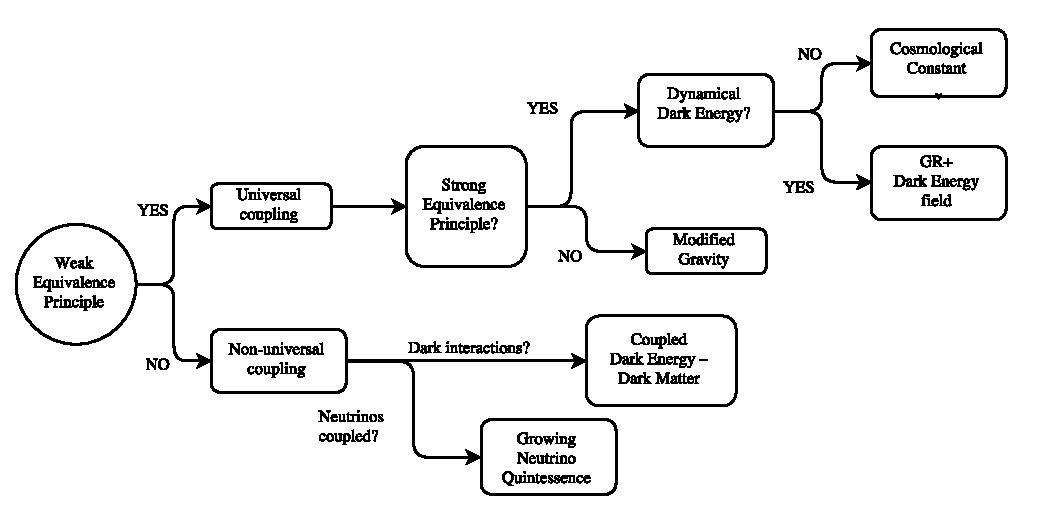
\includegraphics[width=0.99\textwidth]
		{Figures/DE-MG.pdf}
	\end{center}
	\caption[Dark Energy - Modified Gravity Flowchart]{Distinction between Dark Energy and
		Modified Gravity Theories based on the Strong and Weak Equivalence Principles (SEP and WEP), according to \cite{joyce_dark_2016-2}.
		The violation of the SEP, implies the existence of an extra fifth-force among particles, 
		or, equivalently, a modification of the standard Poisson equation. These are the so-called Modified Gravity theories.
		If the scalar degree of freedom is not coupled to matter, then we can talk about a Dark Energy model.
		In the case in which Dark Energy is not dynamical, the theory goes back to GR plus a cosmological constant.
		If the WEP is violated, then not all matter species feel the same gravitational forces and therefore
		there can be either dark sector interactions or neutrino--scalar-field interactions.
	}\label{fig:DE-vs-MG-WEP-SEP}
\end{figure}
%The term 
%Modified Gravity can encompass these but also other much more exotic modifications of GR, 
%for example involving extra dimensions and other 
%vector or tensor fields \cite{cite, bigravity, LH vector theory, dgp}. 
Furthermore, independent of the type of coupling to matter,
one can define two frames in which to study these theories. 
In the so-called Einstein frame, the action contains the standard Einstein-Hilbert term $R$,
plus a kinetic and a potential term for the scalar field $\phi$. 
However, particles are coupled to a metric that in principle depends also on the scalar field. 
On the other hand, in the Jordan frame, the scalar field $\varphi$ is non-minimally coupled
to gravity, which means that in place of the Ricci scalar,
there is a general function $f(R,\varphi)$. Besides, one can also have a potential
and kinetic term for the scalar field. 
The Einstein-Hilbert term is modified, but particles feel a metric that is purely of geometrical origin. 
We will specify the equations for these two different frames in
\cref{sec:Einstein-Jordan} below.
%but 
%One can regard this extra degree of freedom as an exotic new form of matter, affecting the right hand side of the Einstein field equation \ref{eq:Einstein-field-equations} and generally coupled in distinct ways to different matter fields, 
%or one can consider gravity to have an extra degree of freedom coupled non-minimally to the 
%Ricci scalar and therefore modifying 
%directly the left hand side of Einstein's field equations. The latter frame of reference
%is called the Jordan frame, while the former is usually called the Einstein frame.

%For theories in which all matter fields are coupled in the same way to the scalar field, both descriptions
%have to be equivalent and we call them \emph{universally coupled} theories. 
%For theories in which the coupling is specific to a matter field (i.e. neutrinos), the theory 
%is usually formulated in the Einstein frame. These are the so-called \emph{non-universally} coupled theories.
%In the following, we will use this classification to discuss the models studied in this work.

The distinction between Modified Gravity and Dark Energy is somewhat diffuse, since as mentioned above, 
an exotic form of matter in the Einstein's equations can always be considered as a modification 
of involving geometry. However, we will use a definition introduced recently by \cite{joyce_dark_2016-2}, 
which is quite practical in terms of its observable properties. 

In this definition, Dark Energy encompasses models which respect both the Weak and the Strong Equivalence
Principles and therefore do not involve extra fifth-forces that act between particles besides gravitational 
interactions (and the other three fundamental forces of nature). 
Modified Gravity encompasses models where the Strong Equivalence Principle is violated and therefore 
bodies can have an extra "scalar charge" that leads to the appearance of a fifth force among them.
In non-universally coupled theories, the Weak Equivalence Principle is violated,
since test bodies would feel different accelerations depending on
their composition. Usually, in these models baryons are uncoupled and therefore they might be called ``dark sector interaction`` theories.


The term ``modified gravity`` is also more general and it is used for
any theory beyond GR that is able to explain the cosmological history
of the Universe. This can include extra dimensions \cite{deffayet2002accelerated},
massive bimetric gravities \cite{akrami2015bimetric, konnig2014stable} or Lorentz-violating theories
\cite{blas2011models}. However, these models are out of the scope of this dissertation. 
For the rest of this work, when we mention Modified Gravity, we will refer to our definition according
to our discussion above and the diagram \ref{fig:DE-vs-MG-WEP-SEP}.

%In the first \cref{sec:universal-coupling} we will discuss universally coupled theories, which include ---among many others--- Quintessence, f(R),
%Scalar-Tensor theories and the Horndeski theory 
%(see \cite{Luca, Cliffton, Silvestri, Joyce, and more} for comprehensive reviews on Modified Gravity theories). 
%We will also discuss
%more general modifications of gravity which are based on the Effective Field Theory (EFT) approach to
%Dark Energy and parameterizations of modifications of gravity, which
%are not connected to any particular model and can accommodate any deviation from standard GR, at least at the linear 
%level in perturbation theory.
%
%In the second section, we will deal with two specific non-universally coupled models of dark energy used in this work. 
%The first one is
%called Coupled Dark Energy (CDE), which only couples the DE field to dark matter particles and leaves baryons uncoupled, therefore respecting solar system
%constraints on gravity.
%The second one, called Growing Neutrino Quintessence (GNQ), is a model in which the neutrino mass is coupled to the DE scalar field, while 
%all other species remain uncoupled, which is a very phenomenologically rich theory, but possesses theoretical difficulties due to its highly non-linear evolution.
%We will explain the motivations for each of these models and we will emphasize their differences in the predictions for structure formation and the background evolution of the Universe.
 
\section{The Einstein and the Jordan frames \label{sec:Einstein-Jordan}}

In this section we will review the form of the action for scalar-tensor theories in the Einstein and Jordan frames,
which are going to be useful concepts in the following chapters. For the moment we will work in units where the reduced Planck mass
$M_{Pl}^{2} = 1/(8 \pi G)$ is equal to unity.

A scalar-tensor theory can be formulated in the "Jordan frame" as:
\beeqalsp$\label{eq:jordan-frame-action}
\mathcal{S} =& \int \dx{4}{x} \sqrt{-g} \left[  \frac{1}{2} F(\varphi, R) - \frac{1}{2} K(\varphi) g^{\mu \nu}  \partial_{\mu}\varphi \partial_{\nu}\varphi 
- U(\varphi)    \right]  \\
& -\int \dx{4}{x} \sqrt{-g} \mathcal{L}^i_m (g_{\mu \nu} , \varPsi^i_m \zeta^{i}(\varphi)) \quad ,
$
where an index $i$ in the matter sector stands for each of the matter species in the Universe. 
In the case of universal coupling, all matter species ``feel`` the same metric $g$, 
 and are are coupled in the same way to the scalar field, through the function
 $\zeta^{i}(\varphi)$. 
In this frame, the Ricci scalar is non-minimally coupled to the field $\varphi$ through a function $F(R, \varphi)$ and, in general, 
can also contain a potential term for $\varphi$ with an extra function $K(\varphi)$ multiplying the kinetic term of the scalar field.
Matter particles follow the standard geodesics of GR and the energy momentum tensor of the matter species is covariantly conserved.

We can relate the Jordan to the Einstein frame, by doing a conformal transformation of the metric $g$, where
this transformation is defined as:
\beeqc$
\tilde{g}^{(i)} = \Omega^2(\phi, R) g
$
and $\Omega^2(\phi, R)$ is a function of the scalar field and ---in the most general case--- of the Ricci scalar, given by
\beeqp$
\Omega^2(\varphi,R) \equiv \parder{F}{R} 
$
Then, the scalar-tensor action in the `Einstein-frame` takes the following form:
\beeqc$\label{eq:einstein-frame-action}
\mathcal{S} = \int \dx{4}{x} \sqrt{-\tilde{g}} \left[  \frac{1}{2} \tilde{R} - \frac{1}{2} \tilde{g}^{\mu \nu}  \partial_{\mu}\phi \partial_{\nu}\phi 
- V(\phi)    \right] - \int \dx{4}{x} \sqrt{-\tilde{g}} \mathcal{L}^i_m (\tilde{g}^{(i)}_{\mu \nu} , 
\varPsi_m^{(i)} \tilde{\zeta}^{i}(\phi) )
$
where a tilde stands for the conformally transformed quantities.
In the case of universal coupling (see \cref{sec:universal-coupling} below), all matter species would couple to the same function $\tilde{\zeta}^{i}(\phi)$. 
If there is non-universal coupling (see \cref{sec:nonuniversal-coupling} below) each species would
have a different function $\tilde{\zeta}^{i}(\phi)$ or be totally uncoupled from the
field with $\tilde{\zeta}^{i}(\phi) = 1$. 
The Einstein frame is defined as the 
frame in which the gravitational part of the action looks standard, since the Ricci scalar appears without multiplicative factors.
In this formulation, the energy-momentum $T^{(m)}_{\mu \nu}$ of the coupled matter species is not conserved, but rather
the sum of the energy momentum tensor of matter and the scalar field $T^{(m+\phi)}_{\mu \nu}$ is the conserved quantity.

For non-relativistic particles this field dependent function $\zeta(\phi)$ can be also absorbed into the mass $m=m(\phi)$, giving rise to particles with varying mass, as we will see below.
This field dependent mass can also be linked to an extra "fifth-force", 
with a coupling strength $Q$
defined by:
\beeqc$\label{eq:definition-of-coupling-Q}
Q(\phi) \equiv -\frac{1}{2}\frac{\partial \ln f}{\partial \phi}
$
where, in these theories, the function $F$ above takes the form: $F(\varphi, R) = f(\varphi)R-2U(\varphi)$, where
$f$ and $U$ are free functions of the field.
To go from the Jordan frame action \cref{eq:jordan-frame-action} to the Einstein frame action
\cref{eq:einstein-frame-action} and at the same time keep a \emph{canonical} kinetic term,
($1/2 \nabla^2 \phi$), a field redefinition has to be performed:
\beeq$
\phi = \int \dx{}{\varphi} \sqrt{(3/2)(f_{,\varphi}/f)^2 + K/f}
$
where the potentials $U$ and $V$ are related by $V = U/f^2$.


For non-universal coupling, we will see two examples of theories formulated in the Einstein frame in \cref{sub:CDE} and \cref{sub:GNQ}.
In \cref{sub:CDE} we will see an example of a constant coupling and in \cref{sub:GNQ} we will see an example of a field-dependent coupling, 
giving rise to very different phenomenologies.

For conformally-invariant theories (those theories in which null-geodesics are not modified by conformal transformations), the conformal factor
just depends on the scalar field and can be written as $\Omega^2(\varphi)=\exp(2\varphi)$. 
This can be seen by performing the transformation $g \rightarrow e^{2\varphi} g$ and 
observing that, at first order in the
scalar field and the gravitational potentials, $\Phi \rightarrow \Phi-\varphi$ and $\Psi \rightarrow \Psi+\varphi$, leaving 
the Weyl (lensing) potential $\Phi_{\rm Weyl} = (1/2)(\Psi + \Phi)$ invariant.
These theories are interesting, since they do not affect gravitational lensing observations,
but still can provide interesting non-standard features in the clustering of matter.


We have to emphasize that physical measurable quantities have to be frame-independent by definition,
since this frame transformation amounts to nothing more than a coordinate and field redefinition 
and one of the principles of the GR formalism which we are not abandoning
is diffeomorphism invariance, which ensures that 
the theory is invariant under general coordinate transformations.


\section{Universal coupling to matter \label{sec:universal-coupling}}

Scalar-tensor theories with universal coupling written in the Jordan frame \cref{eq:jordan-frame-action}, 
encompass many of the most widely studied dark energy and modified gravity models in the literature. 
For example, $f(R)$ theories \cite{de2010f} are recovered when $F(R,\varphi) = f(R)$ and $K=0$;
Brans-Dicke theory \cite{brans1961mach} is recovered when $F(R,\varphi) = \varphi R $ and 
$K(\varphi) = \omega_{BD}/\varphi$, where $\omega_{BD}$ is the Brans-Dicke parameter and finally "k-essence" 
\cite{armendariz2001essentials} is the case in which $F(R,\varphi) = R$ and $K$ can be a general
function of $\varphi$ and its kinetic term $(\nabla \varphi)^2$. 

There are also other theories of modified gravity with a scalar field, that are not encompassed in the set of "scalar-tensor"
theories and that have gained a lot of attention recently. Namely, Galileons \cite{deffayet2011k}, Horndeski \cite{deffayet2013formal} 
and Beyond-Horndeski theories \cite{gleyzes2015exploring}. 
These theories are universally coupled to matter, are formulated
in the Jordan frame and cannot be expressed in the Einstein frame by a conformal transformation, since they contain much more complicated
derivative interactions, for example free functions of $\Box \varphi$ (see \cite{zumalacarregui2014transforming}), where the ``box operator`` is defined as $\Box \equiv g^{\munu}\partial_{\mu}\partial_{\nu}$.

Horndeski's theory \cite{horndeski_original} is an interesting case, since it is the most general theory of 
a scalar field coupled to a metric, with second order equations of motion and free of ghost instabilities. 
This theory was first formulated by Horndeski in the 1970's \cite{horndeski_original}, in a purely mathematical way and was re-discovered by \cite{deffayet2013formal}
and others, at the beginning of the present decade, in the context of Galileon scalar fields. The simplest Galileon model, the so-called cubic Galileon, has a Lagrangian of the form:
$\mathcal{L} \propto R/2 - (\partial \varphi)^2 - (1/\Lambda_3)\Box \varphi (\partial \varphi)^2$, 
where $ \Lambda_3 $ is a free scale that can be set in the theory. The term Galileons, comes from the fact that
these theories are the more general theories, which are invariant under a general Galiliean transformation of the field $\varphi \rightarrow \varphi + b_\mu x^\mu +c$.
Beyond-Horndeski theories are extensions of Horndeski that have higher than second order equations of motion, when expressed 
in the Newtonian gauge, but where the propagating scalar degree of freedom still obeys second order differential equations, avoiding
instabilities, see
\cite{gleyzes2015exploring} and \cite{zumalacarregui2014transforming} for more details on this direction of research.

For the purposes of this work, we will now detail one of the oldest models of Dark Energy, namely
the Quintessence model \cite{ratra_cosmological_1988, wetterich_cosmology_1988} and its extension
Coupled Quintessence introduced by \cite{Amendola_2000}.

Later on we will deal with general modifications of gravity, whose
effect on structure formation can be parameterized by two functions of
scale and time. Finally we will shortly explain one of the most general approaches
to construct theories of modified gravity at linear order; the so-called Effective Field Theory of Dark Energy. We will show also its connection to Horndeski's theory.

\subsection{Quintessence \label{sub:quintessence}}

The Quintessence model
%, which takes its name from the Latin word for "fifth element"
%is one of the oldest models of Dark Energy. It 
was introduced by several authors almost 30 years
ago \cite{ratra_cosmological_1988, wetterich_cosmology_1988},
motivated by studying the 
breaking of scale invariance, which could give rise to a dynamical cosmological constant.
Its Lagrangian is of the form \cref{eq:jordan-frame-action}, with
$F(\varphi, R) = R$, $K = 1$ and a potential $U(\varphi)$.
Since this is a homogeneous field without couplings, we can find its energy density and its pressure 
straightforwardly from the energy-momentum tensor of a perfect fluid in a FLRW background:
\begin{align}\label{eq:quintessence-rho-p}
&\rho_{\varphi} = -T^{0 (\varphi)}_0 = \frac{1}{2}\dot\varphi^2 + U(\varphi) \quad 
&p_{\varphi} = \frac{1}{3} T^{i (\varphi)}_i = \frac{1}{2}\dot\varphi^2 - U(\varphi) \quad ,
\end{align}
which yields the equation of state:
\beeqp$
w_\varphi  = \frac{p_{\varphi}}\rho_{\varphi} = \frac{\dot\varphi^2 - U(\varphi)}{\dot\varphi^2 + U(\varphi)}
$
We can see that for obtaining the required behavior of $w\approx -1$ at late times, in order to fit 
the observations of the expansion of the Universe, we need that the kinetic term $\dot\varphi^2$
becomes much smaller than the potential term $U$.
From the continuity equation for a perfect fluid or from the variation of the action with respect to $\varphi$,
we can find the Klein-Gordon equation for this field:
\beeqp$
\label{eq:Klein-Gordon-Quintessence}
\ddot \varphi + 3 H \dot \varphi + U_{,\varphi} = 0
$
The dynamics and the phenomenology of this model are entirely determined by the shape of the potential
and for this there are many possibilities (see \cite[chap. 7]{amendola_dark_2010}, for a comprehensive review).
The most interesting solutions, which can alleviate the cosmological coincidence problem, are those in which the field
tracks the evolution of matter at early times ($w_\varphi \approx 1$) and then 
evolves towards an attractor (effectively being independent of initial conditions) 
at late times, which yields cosmic acceleration with $w_\varphi \approx -1+\xi$.
The parameter $\xi$ is a combination of parameters entering the potential function $U(\varphi)$ and allows
to distinguish Quintessence from a simple cosmological constant at present time.
The most studied potentials are the exponential potential $U(\varphi) = U_0\exp(-\lambda \varphi)$ 
(see \cite{copeland_exponential_1998}), where $\lambda$ is a free parameter
and the inverse power-law potential $U(\varphi) = M^{4+n} \varphi^{-n}$,
where $M$ is a mass scale of the theory.

Due to the so low energy density of dark energy ($\rho_{DE} \approx 10 ^{-120} M_{Pl}$)
compared to typical energies appearing in particle physics, it is not so easy to construct a 
viable model of Quintessence which is motivated by a fundamental theory. Nevertheless, there are 
some succesful approaches like fermion condensates, Pseudo-Nambu-Goldstone models and 
dilatonic quintessence (see \cite{amendola_dark_2010} and references therein).
These models have to satisfy that at present times dark energy is the dominating 
energy density in the Universe and therefore from the Friedmann equation and \cref{eq:quintessence-rho-p}:
\beeqp$
U(\varphi_0) \approx H_0^2 M_{Pl}^2
$
If we take an inverse power law potential, $U(\varphi) = M^{4+n} \varphi^{-n}$, and take the field to be at present $\varphi_0 = M_{Pl}$,
this would yield a mass scale $M$ of the order
of:
\beeqc$
M \approx H_0^{2/(4+n)} M_{Pl}^{(2+n)/(4+n)}
$
where, with $H_0 \approx 10^{-42} \mathrm{GeV} $, we get a mass scale of $M \approx 10^{-1} \mathrm{GeV}$
for $n=2$, which is a scale compatible with Standard Model particles.
Moreover, to satisfy the requirement of acceleration today, 
the slow-roll condition (analogous to the one in inflation \cite{bartolo_non-gaussianity_2004}) must satisfy 
$ \frac{M_{Pl} V_{,\varphi \varphi}}{V(\varphi_0)} \lessapprox 1$.
Defining the mass of the scalar field $m_\varphi$ as the second derivative of the potential with respect to the field,
$m^2_\varphi \equiv  V_{,\varphi \varphi} $, yields a condition for the scalar field mass:
\beeqp$
m_\varphi \lessapprox H_0 \approx 10^{-33} \mathrm{eV}
$
So in order to be compatible with observations, 
the scalar field mass must be extremely small.
This could cause problems for quintessence models,
since the stability of such small masses is not always guaranteed under radiative corrections \cite{kolda1999quintessential}.

\subsection{Coupled Quintessence \label{sub:CQ}}

It is also interesting to observe the effects of a coupling between the 
scalar field and the matter species.
In \cref{eq:definition-of-coupling-Q} we already saw how from a general
Scalar-Tensor theory, a coupling between matter species and 
the field can arise from an action like the one in \cref{eq:jordan-frame-action}.
However, the matter equations of motion and the Klein-Gordon equation become more tractable if
we make a conformal transformation into the Einstein frame, where
the scalar field Lagrangian will be canonical, but matter will
be coupled to a metric that contains a function of the field $\phi$.
In this case, as stated before, the individual energy-momentum tensors will not
be conserved:
\beeqal$\label{eq:Tmunu-for-CQ}
&\nabla_{\mu} T^\mu_{\nu (\phi)} = -Q T_m \nabla_{\nu}\phi \quad & \nabla_{\mu} T^\mu_{\nu (m)} = +Q T_m \nabla_{\nu}\phi \;\;,
$
where $Q$ is the coupling function and $T_m$ the trace of the energy-momentum tensor of matter. Through the 
conformal transformation the field should also be coupled to radiation, since radiation also feels gravity, 
but since the trace of the energy-momentum tensor of radiation vanishes identically, it does not appear in the 
conservation equations.
In general,
the coupling $Q$ can be different for baryons and for dark matter.
The coupling to baryons is severely constrained by local gravity experiments (see \cite{Agashe:2014kda})
and therefore uncoupling the baryons from the theory 
can yield a model compatible with observations as we will see below for the Coupled Dark Energy model in \cref{sub:CDE}.

If all matter fields are coupled, then some screening mechanism
has to be invoked in order to pass the stringent Solar System and local gravity constraints.
One possibility is the chameleon mechanism (see the book by \citetitle{amendola_dark_2010}, for a comprehensive review), which
is a coupled quintessence field whose effective potential (and therefore its effective mass)
changes according to the environment it is in.
These kind of theories can arise from an action like in \cref{eq:jordan-frame-action},
with $F(\varphi,R) = \exp(-2Q\varphi)R$ and $K(\varphi) =(1-6Q^2)\exp(-2Q\varphi)R$.
For each distribution of matter, taken to be spherically symmetric for simplicity, 
one has to calculate the profile of the field $\varphi (r)$ as a function of the radius $r$,
and one can tune the parameters in such a way that the effective coupling $Q_{\rm eff}$
in a certain region is much smaller than the bare coupling $Q$ appearing in the action.
In this way one can recover for star systems and galaxies the Newtonian predictions.
For more details on these calculations, see \cite{amendola_dark_2010}, chapter 8.4.



\subsection{Effective Field Theory of Dark Energy and Horndeski Theory \label{sub:EFT-of-DE}}

Until now we have treated Dark Energy and Modified Gravity in a rather phenomenological way,
adding a scalar field with an kinetic term, a coupling and a potential without a clear understanding
of which terms are allowed or not.
Recently, there have been substantial efforts by many authors to build an effective field theory 
of dark energy and modified gravity that encompasses all possible terms that are allowed 
in the action at second order (see \cite{Gubitosi2013, Gleyzes2016, bloomfield_dark_2013}). Considering only one extra dynamical
scalar field, respecting the symmetries of homogeneity and isotropy and following the Weak Equivalence Principle (WEP),
this theory can be uniquely formulated. Its action in the Jordan frame (and written in conformal time $\tau$) takes the form:
\begin{align}\label{eq:EFT-action}
\begin{split}
S ={}& \int \dx{4}{x} \sqrt{-g} \left[ \frac{M_{Pl}^2}{2} [1 + \Omega(\tau)] R + \Lambda(\tau) -a^2 c(\tau)\delta g^{00} \right. \\
     & + \frac{M_{2}^4 (\tau)}{2}(a^2 \delta g^{00})^2 -\bar{M}_{1}^3 (\tau) 2 a^2 \delta K^\mu_\mu \delta g^{00} \\
     & - \frac{\bar{M}_2^2 (\tau)}{2} (\delta K_\mu^\mu )^2 - \frac{\bar{M}_3^2 (\tau)}{2}\delta K^{\mu}_{\nu}\delta K^{\nu}_{\mu} \\
     & + a^2 \frac{\hat{M}^2 (\tau)}{2} \delta g^{00} \delta R^{(3)} \\
     & + m^2_2(\tau) (g^{\mu \nu} + n^\mu n^\nu) \partial_{\mu} (a^2 g^{00})\partial_{\nu} (a^2 g^{00}) \\
     & \left. + \mathcal{L}_m(g_{\mu \nu}, \varPsi_m) \right] \quad.
\end{split}
\end{align}
To construct this action, the spacetime has been foliated (similarly to the 3+1 ADM decomposition) into a time direction
and spatial hypersurfaces that coincide with the uniform scalar field hypersurfaces (this is the so-called unitary gauge). 
The preferred time direction is then (c.f. \cite{Gubitosi2013})
\beeqc$
n_\mu \equiv -\frac{\partial_{\mu}\phi}{\sqrt{-(\partial \phi)^2}}
$
which induces a spatial metric $h_{\mu \nu} \equiv g^{\mu \nu} + n^\mu n^\nu $, a spatial Ricci scalar $R^{(3)}$
and defines an extrinsic curvature:
\beeqp$
K_{\mu \nu} \equiv h^{\sigma}_{\mu} \nabla_{\sigma} n_\nu
$
The rest of the terms in the EFT action \cref{eq:EFT-action} are nine free functions of time:\\
$\{\Omega(\tau), \Lambda(\tau), c(\tau), M_{2}^4 (\tau), \bar{M}_{1}^3 (\tau), \bar{M}_2^2 (\tau), \bar{M}_3^2 (\tau),
 \hat{M}^2 (\tau), m^2_2(\tau)\}$, whose choice specify the theory.
This theory encompasses all theories of an extra dynamical scalar field, which respect the WEP.
At the linear level in perturbations, it includes the Horndeski theory (mentioned above in \cref{sec:universal-coupling}) 
and also theories which go beyond second order equations of motion (in the Newtonian gauge), also called
Beyond-Horndeski theories (see \cite{gleyzes2015exploring})

Since these theory involves many free functions, we need to choose a parametrization for each of them and 
we need to take some simplifying assumptions in order to be able to constrain this theory with data.
Recently, a code capable of calculating the linear Einstein-Boltzmann system of equations for the EFT formalism
has been made public, the so-called \textsc{EFTCAMB} (\cite{hu_effective_2014, hu_eftcamb/eftcosmomc:_2014-2}), which is based 
on the widely used \textsc{CAMB} code by\cite{lewis_efficient_2000}. 
We will use this code to calculate the observables which we will 
implement into our Fisher forecast in \cref{sec:EFT-forecasts}.

Furthermore, we will use the assumptions taken in \cite{planck_collaboration_planck_2016} in order to simplify
the theoretical modeling.
If we assume a $\lcdm$ background, and choose freely a function
$\Omega(\tau)$, the functions $\Lambda(\tau) \textrm{ and } c(\tau)$ are then fixed \cite{hu_effective_2014}.
Furthermore, we will impose $ m^2_2(\tau) = 0$ and $ \bar{M}_2^2 (\tau) = - \bar{M}_3^2 (\tau)$,
which eliminates models which contain third-order spatial derivatives.
Now we just have 5 free functions of time and a function specifying the background cosmology $H(\tau)$.
These free functions of time can be mapped to the Bellini-Sawicki $\alpha_i (\tau)$ 
functions (see \cite{bellini_maximal_2014}),
which fully specify the evolution of Horndeski models at linear order in perturbation theory. The following relations between the EFT functions and the $\alpha$ functions hold:
\beeqal$ \label{eq:EFT-funcs}
\begin{split}
M_{*}^2 (\tau) & = M_{Pl}\Omega(\tau) + \bar{M}_2^2 (\tau) \\
M_{*}^2 (\tau) H(\tau) \alpha_M (\tau)   & = M_{Pl}\dot{\Omega}(\tau) + \dot{\bar{M}}_2^2 (\tau) \\
M_{*}^2 (\tau) H^2(\tau) \alpha_K (\tau)   & = 2 c (\tau) + M_2^4 (\tau) \\
M_{*}^2 (\tau) H(\tau) \alpha_B (\tau)   & = M_{Pl}\dot{\Omega}(\tau) - \bar{M}_{1}^3 (\tau)\\
M_{*}^2 (\tau) \alpha_T (\tau)   & = - \bar{M}_2^2 (\tau) \\
M_{*}^2 (\tau) \alpha_H (\tau)   & = 2 \hat{M}^2(\tau) - \bar{M}_2^2 (\tau)
\end{split}
$ 
Here, the bare reduced Planck mass is $M_{Pl}$ and the effective Planck mass is $ M_{*}^2 $.
These $\alpha_i$ functions are much easier to interpret physically than the EFT functions.

The first four $\alpha_i$ functions, $\alpha_M$, $\alpha_K$,
$\alpha_B$ and $\alpha_T$  describe fully the physics
of linear perturbations in Horndeski's theory (see \cite{bellini_maximal_2014}).
For instance, $\alpha_M$ (\emph{mass run rate}) is the rate of change of the effective Planck mass, 
produces anisotropic stress; $\alpha_K$ (\emph{kineticity}) is present in Quintessence (\cref{sub:quintessence}) models, 
but also in models where the scalar field has a non-zero sound speed, like k-essence models;
$\alpha_B$ (\emph{braiding}) causes dark energy to cluster and $\alpha_T$ is the \emph{tensor speed excess}, which gives the deviation
of the speed of gravitational waves from that of light.
Finally $\alpha_H$ is a term indicating physics that lies beyond the Horndeski models at linear level. 
For our results in \cref{sec:EFT-forecasts}, we will further reduce this theory to a simpler case, 
which can be compared easier with Large-Scale-Structure observations.


\subsection{Parameterizing Modified Gravity \label{sub:parameterizing-MG}}

In the previous sections we have seen how to construct Dark Energy and Modified Gravity theories 
which have an extra scalar degree of freedom, besides the Einstein-Hilbert term and the matter and radiation species.
As we have seen, one can successfully construct the most general theory of this kind, by either imposing
some conditions on the equations of motion and the stability of the theory (as in Horndeski theories) or by considering all
possible terms allowed by symmetries in the second order action (as in EFT).

However, for observations, these general theories are not so practical, since there is not enough data to constrain
all the free functions in the Lagrangian. What we really can observe with Galaxy Clustering and Weak Lensing 
are the perturbations of matter $\delta_m(z,k)$, its correlation function across scales $P_m(z,k)$ and the
evolution of matter structures in time, $f(z)$.
In Einstein-GR, these three quantities are determined by the gravitational potentials $\Phi$ and $\Psi$, which follow 
the general relativistic Poisson equations (see \cref{eq:relativistic-Poisson}). 
In linear perturbation theory, scalar, vector and tensor perturbations
do not mix, which allows us to consider only the scalar perturbations of the metric. 
We work in the conformal Newtonian gauge, with the
line element given by \cref{eq:linearized-metric-scalar}
%\begin{equation}
%ds^{2}=-(1+2\Psi)dt^{2}+a^{2}(1-2\Phi)dx^{2}\,\,\,.
%\end{equation}
The potentials $\Phi$ and $\Psi$ are in functions of time and in our notation, they coincide
with the gauge-invariant Bardeen potentials.

%In modified gravity, it has been shown that
%the deviations from Einstein-GR can be fully described by 
%two generic free functions of time and space \cite{kunz_phenomenological_2012, amendola_observables_2013}.
%While any two (independent) functions of the gravitational potentials would be suitable, 
%we consider in this work the most common parameterization (see \cite{planck_collaboration_planck_2016}) given by $\mu(a,k)$ and $\eta(a,k)$: the first modifies the Poisson equation for $\Psi$ while the second is equal to the ratio of the gravitational potentials and is therefore also a direct observable \cite{amendola_observables_2013}.

%In section \ref{sec:Parameterizing-Modified-Gravity} we define $\mu$ and $\eta$ and parameterize them in three different ways. First, in a general manner, we let these functions vary freely in different  redshift bins. Complementarily, we also consider two specific parameterizations of the time evolution proposed in \cite{planck_collaboration_planck_2016}. Here, we also specify the fiducial values of our cosmology for each of the
%parameterizations considered.

In theories with an extra scalar degree of freedom (see the discussion around \cref{fig:DE-vs-MG-WEP-SEP} for a distinction between Dark Energy and Modified Gravity)
the standard linear perturbation equations
are no longer valid, so that for a given matter source the values
of $\Phi$ and $\Psi$ will differ from their Einstein-GR values (see \cite{kunz_phenomenological_2012, amendola_observables_2013}). We can
parameterize this change generally with the help of two new functions $\mu(a,k)$ and $\eta(a,k)$
that encode the modifications. Many different choices are possible
and have been adopted in the literature, see e.g. \cite{planck_collaboration_planck_2016} for a limited overview. 
In this work
we introduce the two functions through a gravitational slip (leading
to $\Phi\neq\Psi$ also at linear order and for pure cold dark matter)
and as a modification of the Poisson equation for $\Psi$, 
\begin{align}
-k^{2}\Psi(a,k) & \equiv  4\pi
Ga^{2}\mu(a,k)\rho(a)\Delta(a,k)\,\,\,;\label{eq:mu_def}\\
\eta(a,k) & \equiv \Phi(a,k)/\Psi(a,k) \quad \label{eq:eta_def}.
\end{align}
These expressions define the modified gravity functions
$\mu$ and $\eta$. Here $\rho(a)$ is the average dark matter density and $\delta(a,k)$
the comoving matter density contrast -- we will neglect relativistic
particles and radiation as we are only interested in modeling the
perturbation behaviour at late times. 
In this formulation, $\eta$,
which is effectively an observable \cite{amendola_observables_2013}, is closely related to
modifications of GR \cite{saltas_anisotropic_2014,sawicki_non-standard_2016}, 
while $\mu$ encodes for example deviations in
gravitational clustering, as non-relativistic particles are accelerated by the gradient of $\Psi$.

When considering Weak Lensing observations then it is also natural
to parameterize deviations in the lensing or Weyl potential $\Phi+\Psi$,
since it is this combination that affects null-geodesics.
To this end we introduce a function $\Sigma(a,k)$ so that
\begin{equation}\label{eq:Sigma-def}
-k^{2}(\Phi(a,k)+\Psi(a,k))\equiv8\pi
Ga^{2}\Sigma(a,k)\rho(a)\delta(a,k) \quad .
\end{equation}
Since metric perturbations are fully specified by two functions of
time and scale, $\Sigma$ is not independent from $\mu$ and $\eta$,
and can be obtained from the latter as follows: 
\begin{equation}\label{eq:SigmaofMuEta}
\Sigma(a,k)=(\mu(a,k)/2)(1+\eta(a,k)) \quad.
\end{equation}
Throughout this work, we will denote the standard Lambda-Cold-Dark-Matter ($\Lambda$CDM) model,
defined through the Einstein-Hilbert action with a cosmological constant, simply as Einstein-GR, where $\mu=\eta=\Sigma=1$. 
If only $\mu$ deviates from unity at late times,
it indicates either Modified Gravity or just a Dark Energy field that clusters.
If $\eta$ deviates from unity, it is an indication for Modified Gravity models, according to our definitions above \cref{fig:DE-vs-MG-WEP-SEP}, based on \cite{joyce_dark_2016}.


Using effective quantities like $\mu$ and $\eta$ has the advantage
that they are able to model {\em any} deviations of the perturbation
behaviour from $\Lambda$CDM expectations, they are relatively close 
to observations, and they can also be related to other commonly used 
parameterizations \cite{pogosian_how_2010}.
On the other hand, they are not
easy to map to an action ---as opposed to approaches like Effective
Field Theory (EFT, \cref{sub:EFT-of-DE})---  and in addition they
contain so much freedom that we normally restrict their parameterization
to a subset of possible functions.


\subsubsection{Parameterizing gravitational potentials with simple smooth functions of the scale factor \label{sub:param-smooth-funct}}

The first possibility is to assume simple specific time parameterizations for
the $\mu$ and $\eta$ functions, adopting the ones used in the
\planck\ analysis \cite{planck_collaboration_planck_2016}, where we neglect here any scale dependence:
\begin{itemize}
	\item a parameterization in which the time evolution is related to the dark
	energy density fraction, to which we refer as `late-time' parameterization:
	\beeqal$
	\mu(a,k) \equiv& \; 1+E_{{\rm 11}}\Omega_{{\rm
			DE}}(a)  \quad ,\label{eq:DE-mu-parametrization}\\
	\eta(a,k)\equiv& \; 1+E_{{\rm 22}}\Omega_{{\rm
			DE}}(a)  \quad ;\label{eq:DE-eta-parametrization}
     $
	
	\item a parameterization in which the time evolution is the simplest first
	order Taylor expansion of a general function of the scale factor $a$
	(and closely resembles the $w_{0}-w_{a}$ parametrization for the
	equation of state of DE), referred to as `early-time' parameterization, because it
	allows departures from GR also at high redshifts:
%	\footnote{Notice that our early-time parametrization is called
%		`time-related' in \cite{planck_collaboration_planck_2016}.}:
	\beeqal$
	\mu(a,k)\equiv & \; 1+E_{{\rm 11}}+E_{{\rm
			12}}(1-a)  \quad,\label{eq:TR-mu-parametrization}\\
	\eta(a,k)\equiv & \; 1+E_{{\rm 21}}+E_{{\rm
			22}}(1-a)  \quad.\label{eq:TR-eta-parametrization}
	$	
\end{itemize}
The parameters $E_{i j}$ are usually order-unity parameters, which give the amplitude of the modifications
at present time: $E_{11}$ for $\mu$ and $E_{22}$ for $\eta$ in the late-time parameterization and 
$E_{11}$ for $\mu$ and $E_{21}$ for $\eta$ in the early-time parameterization, while
$E_{12}$ and $E_{22}$ measure the slope of the time-evolution function.


The late-time parameterization is forced to behave as Einstein-GR ($\mu=\eta=1$)
at high redshift when $\Omega_{{\rm DE}}(a)$ becomes negligible;
the early time parameterization allows more freedom as the amplitude of the deviations
from Einstein-GR do not necessarily reduce to zero at high redshifts. 
Both parameterizations have been used in \cite{planck_collaboration_planck_2016}
and in other recent studies of how to constrain Modified Gravity with Galaxy Clustering and Weak Lensing observations, see
\cite{bull_extending_2015, Gleyzes2016} and \cite{Alonso2016}.
In \cref{chap:MG-forecasts} we will study in more detail both the late-time and the early-time parameterizations and we will
try to find out how well future observations will be able to measure $\mu$ and $\eta$, using linear and non-linear
matter perturbations.


\subsubsection{Parameterizing gravitational potentials in discrete redshift bins \label{sub:param-z-bins-th}}

A second and more model-independent approach
is to specify the time evolution of the functions $\mu$ and $\eta$ without
any parameterization.
To this purpose we "pixelize" the functions $\mu$ and $\eta$ at $N$ redshift bins $z_i$, with $i=\{1, \ldots N  \}$ 
and we consider the values
$\mu(z_{i})$ and $\eta(z_{i})$ at the right limiting redshift $z_{i}$
of each bin as free parameters.
The $\mu(z)$ function (and analogously $\eta(z)$) is then reconstructed
as 
\begin{equation}\label{eq:MGbin-mu-general-parametrization}
\mu(z)=\mu(z_{1})+\sum_{i=1}^{N-1}{\frac{\mu(z_{i+1})-\mu(z_{i})}{2}\left[1+\tanh{\left(s\frac{z-z_{i+1}}{z_{i+1}-z_{i}}\right)}\right]},
\end{equation}
where $s=10$ is a smoothing parameter and $N$ is the number of binned
values. We assume that both $\mu$ and $\eta$ reach the Einstein-GR limit
for a redshift higher than $z_h$: to realize this, the last $\mu(z_{N})$ and $\eta(z_{N})$
values assume the standard $\lcdm$ value $\mu=\eta=1$ and both functions
are kept constant at higher redshifts $z> z_h$.


Similarly, the derivatives of these functions are obtained by computing
\begin{equation}
\mu'({\bar{z}_{j}})=\frac{\mu(z_{i+1})-\mu(z_{i})}{z_{i+1}-z_{i}},
\end{equation}
with $\bar{z}_{j}=(z_{i+1}+z_{i})/2$, using the same $\tanh(x)$
smoothing function: 
\begin{equation}\label{eq:MGbin-muderiv-parametrization}
\frac{d\mu(z)}{dz}=\mu'(\bar{z}_{1})+\sum_{j=1}^{N-2}{\frac{\mu'(\bar{z}_{j+1})-\mu'(\bar{z}_{j})}{2}\left[1+\tanh{\left(s\frac{z-\bar{z}_{j+1}}{\bar{z}_{j+1}-\bar{z}_{j}}\right)}\right]}\,\,\,.
\end{equation}
In particular we assume $\mu'=\eta'=0$ for $z<0.5$ and for $z>3$.

This approach has the advantage of being independent of the parameterization of the time evolution of $\mu$ and $\eta$,
but at the cost of introducing
many more parameters that have to be constrained by observations.
Furthermore, one does not know a priori how many binned parameters have to be taken into account
and what are the degeneracies among them.
This will be the subject of study in \cref{chap:MG-forecasts}, where we will
introduce the functions $\mu$ and $\eta$ parameterized in redshift bins and we will forecast
how well future observations will be able to measure those functions.



\section{Non-universal coupling \label{sec:nonuniversal-coupling}}

In \cref{sec:DE-MG-sec} we have motivated the inclusion of a scalar field as a 
way of solving the dark energy problem and alleviating the coincidence problem.
The energy fraction of Dark Energy and that of Dark Matter are of the same
order of magnitude only for a very short period of time in cosmological time scales and that time is precisely
now when we are capable of making observations. This introduces the question if this is just a coincidence or 
if somehow Dark Energy and Dark Matter are connected beyond simple gravitational physics.
Therefore a natural way of alleviating this "coincidence problem" issue (which we discussed in \cref{sub:CC-problem})
is to imagine there is a coupling in the dark sector or some mechanism that connects the onset of non-linear 
structure formation to the epoch of accelerated expansion of the Universe. As we will see, the coupling to baryons 
is extremely well constrained by solar system and galactic observations and therefore a coupling to baryons 
has to be avoided.

In this section we will deal with two non-universally coupled theories which can yield very distinctive 
effects on the formation and evolution of structures in the Universe.
In the first model, called (\cref{sub:CDE}) Coupled Dark Energy, there exists an exchange of energy and momentum
between a quintessence scalar field and the dark matter particles. 
The second one is also a quintessence model, but this time the masses of neutrinos are 
coupled to the scalar field. In this model, the DE domination is triggered by the neutrinos becoming non-relativistic
and their mass is connected to the energy scale attributed to the DE field.

As we have seen before, if the Weak Equivalence principle is violated, then there exists a fifth force acting between test
particles on top of the gravitational interaction. Generally this will yield modifications in the growth rate of perturbations, 
the density profiles of structures and the matter power spectrum. Since the effects appear generally the non-linear regime,
we will have to study them by performing numerically expensive N-body simulations, as we will see in \cref{chap:Fitting-CDE}
and \cref{chap:GNQ}.


\subsection{Coupled Dark Energy \label{sub:CDE}}

We explained in \cref{sub:CQ} how a coupling between all matter species and a scalar field can be realized in the Jordan frame.
However, for non-universal couplings it is easier to work in the Einstein frame, in which the Lagrangian takes the form:
\beeqalsp$\label{eq:CDE-Lagrangian}
\mathcal{L} = \frac{1}{2} \tilde R - \frac{1}{2} \tilde{g}^{\mu \nu}  \partial_{\mu}\phi \partial_{\nu}\phi 
- V(\phi) - m(\phi) \bar{\psi} \psi + \mathcal{L}_{\rm kin}(\psi) \quad,
$
where $\psi$ is the coupled dark matter field, $m$ its mass and $\mathcal{L}_{\rm kin}(\psi)$
its kinetic term.

The coupling to baryons is severely constrained by observations at solar system scales.
The ``post-Einstein'' coupling parameter $\bar{\gamma}$ defined as the quantity that
measures the local admixture of a scalar field to gravity is
constrained in Solar System experiments  roughly to
$|\bar{\gamma}|\le4\cdot10^{-5}$ (see e.g. the PDG review \cite{Agashe:2014kda}
and \citep{Will_2005,Bertotti_Iess_Tortora_2003}). 
This parameter enters the modification
of the effective Newton constant as $G_{eff}=G_{N}(1-\bar{\gamma}/2)$. 
We will see below, that the effective force coming from a coupling to matter is
in our notation, $G_{eff}=G_{N}(1+4\beta^{2}/3)$
and therefore $\beta^{2}=-3\bar{\gamma}/8$. A coupling $\beta_{\rm baryons}^{2}$
appears then constrained to be smaller than $10^{-5}$ roughly, and
we assume therefore that is completely negligible. As a consequence,
baryons follow the usual geodesics of a FLRW cosmology, which allows
coupled DE to pass the stringent local gravity constraints without 
the need to employ any screening mechanism \cite{hamilton_atom-interferometry_2015}, 
\cite{khoury2010theories, bloomfield2015shape}.

The background evolution for the coupled DE scenario model is described
by the following equations, in which the subscripts $r$, $b$, $c$
and $\phi$, indicate radiation, baryons, cold dark matter (CDM) and
the dark energy scalar field, respectively:

\begin{eqnarray}
\ddot{\phi}+3H\dot{\phi}+\frac{dV}{d\phi} & = & \sqrt{\frac{2}{3}}\beta(\phi)\frac{\rho_{c}}{M_{Pl}}\,\,,\label{eq:quint-kleingordon}\\
\dot{\rho}_{c}+3H\rho_{c} & = & -\sqrt{\frac{2}{3}}\beta(\phi)\frac{\rho_{c}\dot{\phi}}{M_{Pl}}\,\,,\label{eq:cdm-back-density}\\
\dot{\rho}_{b}+3H\rho_{b} & = & 0\,\,,\\
\dot{\rho}_{r}+4H\rho_{r} & = & 0\,\,,\\
3H^{2} & = & \frac{1}{M_{Pl}^{2}}(\rho_{b}+\rho_{c}+\rho_{r}+\rho_{\phi})\,\,.
\end{eqnarray}


We express the scalar field $\phi$ in units of the Planck
mass $M_{pl}\equiv1/\sqrt{8\pi G}$, and choose as potential $V(\phi)$
an exponential $V(\phi)=Ae^{-\alpha\phi}$ \citep{Lucchin_Matarrese_1984,Wetterich_1988}.
The coupling function $\beta(\phi)$ defines the strength of the interaction
between the DE fluid and CDM particles and in the present work we
will restrict our analysis to the simplified case of a constant coupling
$\beta(\phi)=\beta$, although in general it could be a field-dependent
quantity \cite{Amendola_2004,Baldi_2011a}.

Due to the exchange of energy between DE and CDM, the energy density
of the latter will no longer scale as the cosmic volume, and by assuming
the conservation of the CDM particle number one can derive the time
evolution of the CDM particle mass by integrating Eq.(\ref{eq:cdm-back-density})
between the present time ($z=0$) and any other redshift $z$:
\begin{equation}
m_{c}(z)=m_{c,0}e^{-\beta(\phi(z)-\phi(0))}\,\,.
\end{equation}


At the level of linear perturbations, coupled DE models are characterized
by a different evolution of the baryonic and CDM density fluctuations,
as a consequence of the selective interaction between DE and CDM particles
only. In the sub-horizon limit, for which $aH/k\ll1$, linear perturbations
in coupled dark energy follow the equations \citep{Amendola_2004,pettorino_baccigalupi_2008}:
\begin{eqnarray}
\ddot{\delta}_{c} & = & -2H\left[1-\beta\frac{\dot{\phi}}{H\sqrt{6}}\right]\dot{\delta}_{c}+4\pi G\left[\rho_{b}\delta_{b}+\rho_{c}\delta_{c}\Gamma_{c}\right]\label{linear_cdm}\\
\ddot{\delta}_{b} & = & -2H\dot{\delta}_{b}+4\pi G\left[\rho_{b}\delta_{b}+\rho_{c}\delta_{c}\right]\label{linear_baryons}
\end{eqnarray}
where $\Gamma_{c}\equiv1+\frac{4}{3}\beta^{2}$ represents the effective
``fifth force'' acting on the CDM particles. The term proportional
to $\beta\dot{\phi}$ in equation (\ref{linear_cdm}) is a velocity-dependent
term that modifies the standard cosmological friction; this arises
as a consequence of momentum conservation for the CDM particles and
has a considerable effect on structure formation \citep{baldi_etal_2010,baldi_clarifying_2011,Li_Barrow_2011}.
Since baryons are uncoupled, their perturbations evolve according
to the standard equation. Nonetheless, baryons will still be indirectly
affected by the coupling as the source term on the right-hand side
of equation (\ref{linear_baryons}) includes the CDM density perturbations.

At the level of non-linear perturbations, several methods have been
devised to predict the small scale effects of coupled DE, from semi-analytical
methods like spherical collapse \cite{Pace_Waizmann_Bartelmann_2010},
to time renormalization group \citep{Saracco_etal_2010} to full N-body
simulations \citep{Maccio_etal_2004,baldi_etal_2010,Li_Barrow_2011,Carlesi_etal_2014a}.
In \cref{chap:Fitting-CDE}, we will work with the publicly available data of
the \textsc{CoDECS} simulations \citep{baldi_codecs_2012}
that represents the largest set of cosmological N-body simulations
for coupled DE models to date.



\subsection{Growing Neutrino Quintessence \label{sub:GNQ}}

Growing neutrino quintessence, developed in \cite{amendola_growing_2008,wetterich_growing_2007}, among others,
explains the end of a cosmological scaling solution (in which dark
energy scales as the dominant background) and the subsequent transition
to a dark energy dominated era by the growing mass of neutrinos, induced
by the change of the value of the cosmon field which is responsible
for dynamical dark energy. 
The dependence of the mass of neutrinos
on the cosmon (dark energy) field $\phi$, 
\begin{equation}
m_{\nu}=m_{\nu}(\phi)\propto\hat{m}_{\nu}e^{-\int\beta(\phi)d\phi}\quad,\quad \beta(\phi)=-\frac{\partial\ln m_{\nu}(\phi)}{\partial\phi}\label{eq: mass_def}
\end{equation}
involves the cosmon-neutrino coupling $\beta(\phi)$ which measures
the strength of the fifth force (additional to gravity). The constant
$\hat{m}_{\nu}$ is a free parameter of the model which determines
the size of the neutrino mass. (We take for simplicity all three neutrino
masses equal - or equivalently $m_{\nu}$ stands qualitatively for
the average over the neutrino species.) The special role of the neutrino
masses (as compared to quark and charged lepton masses) is motivated
at the particle physics level by the way in which neutrinos get masses
(see \cite{wetterich_growing_2007}). Growing neutrino quintessence with
a sufficiently large negative value of $\beta$ successfully relates
the present dark energy density and the mass of the neutrinos. The
evolution of the cosmon is effectively stopped once neutrinos become
non-relativistic. Dark energy becomes important now because neutrinos
become non-relativistic in a rather recent past, at typical redshifts
of about $z=5$ (see \cite{mota_neutrino_2008}). In this way, the ``why
now problem'' is resolved in terms of a ``cosmic trigger event''
induced by the change in the effective neutrino equation of state,
rather than by relying on the fine tuning of the scalar potential.
This differs from other mass varying neutrino cosmologies (usually
known as MaVaN's) \cite{brookfield_cosmology_2007,la_vacca_mass-varying_2013,bi_cosmological_2005,fardon_dark_2004,kaplan_neutrino_2004,spitzer_stability_2006,takahashi_speed_2006}.
Some of the observational consequences of those models were studied
in \cite{la_vacca_mass-varying_2013,kaplan_neutrino_2004} and more
recently a new scalar field - neutrino coupling that produces viable
cosmologies was proposed in \cite{simpson_dark_2016}. A viable cosmic
background evolution of growing neutrino quintessence offers interesting
prospects of a possible observation of the neutrino background.

The case in which the coupling $\beta$ is constant has been largely
investigated in literature at the linear level \cite{mota_neutrino_2008},
in semi-analytical non-linear methods \cite{wintergerst_clarifying_2010,wintergerst_very_2010,brouzakis_nonlinear_2011},
joining linear and non-linear information to test the effect of the
neutrino lumps on the cosmic microwave background \cite{pettorino_neutrino_2010}
and within N-Body simulations \cite{ayaita_neutrino_2013,ayaita_structure_2012,baldi_oscillating_2011,ayaita_nonlinear_2016}.
For the values of $\beta$ ($\beta\gtrsim10^{3}$) needed for dark
energy to dominate today, the cosmic neutrino background is clumping
very fast. Large and concentrated neutrino lumps form and induce very
substantial backreaction effects. These effects are so strong that
the deceleration of the evolution of the cosmon gets too weak, making
it difficult to obtain a realistic cosmology \cite{fuhrer_backreaction_2015}.

In this dissertation we instead consider the case in which the neutrino-cosmon
coupling $\beta(\phi)$ depends on the value of the cosmon field and
changes with time, along the framework of ``varying growing neutrino models''
(see \cite{wetterich_growing_2007, la_vacca_mass-varying_2013}). 

In a particle physics context this has been motivated in 
\cite{wetterich_growing_2007} by a decrease with $\phi$ of the heavy
mass scale (B-L-violating scale) entering inversely the light neutrino
masses in the seesaw mechanism. 
In this scenario $\beta(\phi)$ has not been large in all
cosmological epochs - the present epoch corresponds to a crossover
where $\beta$ gets large. A numerical investigation \cite{baldi_oscillating_2011}
of this type of model has revealed compatibility with observations
for the case of a present neutrino mass $m_{\nu,0}=0.07$ eV. In the
present project we investigate the dependence of cosmology on the value
of the neutrino mass by varying the parameter $\hat{m}_{\nu}$ in
eq. \ref{eq: mass_def}. For large neutrino masses we find a
qualitative behavior similar to the case of a constant neutrino-cosmon
coupling $\beta$, with difficulties to obtain a realistic cosmology.
In contrast, for small neutrino mass, the neutrino lumps form and
dissolve, with small influence on the overall cosmological evolution.
In this case, the neutrino-induced gravitational potentials are found
to be much smaller than the ones induced by dark matter. As we will
discuss in \cref{chap:GNQ}, it will not be easy to find observational signals
for the neutrino lumps. In-between the regions of small and large
neutrino masses we expect a transition region for intermediate neutrino
masses where, by continuity, observable effects of the neutrino lumps
should show up.

As long as neutrinos are relativistic,
the coupling is inefficient and the dark energy scalar field $\phi$
rolls down a potential, as in an early dark energy scenario. As the
neutrino mass increases with time, neutrinos become non-relativistic,
typically at a relatively late redshift $z\approx4-6$ \cite{pettorino_neutrino_2010}.
This influences the evolution of $\phi$, which feels the effect of
neutrinos via a coupling to the neutrino mass $m_{\nu}(\phi)$. The
evolution of the scalar field slows down and practically stops, such
that the potential energy of the cosmon behaves almost as a cosmological
constant at recent times. In other words, in these models the cosmological
constant behavior observed today is related to a cosmological trigger
event (i.e. neutrinos becoming non-relativistic) and the present dark
energy density is directly connected to the value of the neutrino
mass. In the following we will detail the formalism and equations
used to describe the cosmological evolution of the model.

We will use here the linearized Einstein equations, treated in \cref{sub:linearized-Einstein-eqs}, 
but now we have to pay attention to the fact that the term $\delta T_{0}^{0}$ 
(\cref{eq:perturbed-Tmunu}) sourcing the Poisson equation \cref{eq:pertphipsi-1},
will contain contributions from all matter
species (dark matter \& neutrinos) and from the cosmon field, which in this case also clusters.
The total density perturbation will be: $\delta\rho_{t}=\delta\rho_{\nu}+\delta\rho_{m}+\delta\rho_{\phi}$.
Moreover, we cannot neglect the anisotropic stress term $\sigma$ in \cref{eq:pertphipsi-4} which is important for relativistic
particles (i.e. the neutrinos).


The cosmon field can be described through a Lagrangian in the standard
way 
\begin{equation}
-\mathcal{L_{\phi}}=\frac{1}{2}\partial^{\nu}\phi\partial_{\nu}\phi+V(\phi)
\end{equation}
where for this work we choose an exponential potential $V(\phi)\propto e^{-\alpha\phi}$.
The field dependent mass (eq.\ref{eq: mass_def}) allows for
an energy-momentum transfer between neutrinos and the cosmon, which
is proportional to the trace of the energy momentum tensor of neutrinos
$T_{(\nu)}$ and to a coupling parameter $\beta(\phi)$ 
\begin{align}
\nabla_{\eta}T_{(\phi)}^{\mu\eta}= & +\beta(\phi)T_{(\nu)}\partial^{\mu}\phi\,\,\,,\label{eq:continuity-phi}\\
\nabla_{\eta}T_{(\nu)}^{\mu\eta}= & -\beta(\phi)T_{(\nu)}\partial^{\mu}\phi\,\,\,.\label{eq:continuity-nu}
\end{align}


The cosmon is the mediator of a fifth force between neutrinos, acting
at cosmological scales. Its evolution is described by the Klein-Gordon
equation sourced by the trace of the energy-momentum tensor $T_{(\nu)}$
of the neutrinos,

\begin{equation}
\nabla_{\mu}\nabla^{\mu}\phi-V'(\phi)=\beta(\phi)T_{(\nu)}.\label{eq:klein-gordon-equation}
\end{equation}
As long as the neutrinos are relativistic ($T_{(\nu)}=0)$ the source
on the right hand side vanishes. During this time, the coupling has
no effect on the evolution of $\phi$. While the potential term $\sim V'$
drives $\phi$ towards larger values, the term $\sim\beta$ has the
opposite sign and stops the evolution effectively once $\beta T_{(\nu)}$
equals $V'$. The trace of the energy momentum tensor $T_{\nu}$,
entering eq.\ref{eq:klein-gordon-equation} is equal to: 
\begin{equation}
T_{\nu}=m_{\nu}(\phi)\tilde{n}(\phi)\label{eq:trace}
\end{equation}
where $\tilde{n}_{\nu}(\phi)=n_{\nu}(\phi)/\gamma$ is the ratio of
the number density of neutrinos $n_{\nu}$, divided by the relativistic
$\gamma$ factor. Eq.\ref{eq:trace} is valid for both relativistic
and non-relativistic neutrinos. Here we consider a coupling $\beta$
between neutrino particles and the quintessence scalar field $\phi$
as a field dependent quantity: 
\begin{equation}
\beta(\phi)\equiv-\frac{1}{\phi_{c}-\phi}\,.\label{eq:beta-of-phi}
\end{equation}
From eq.\ref{eq: mass_def} the neutrino mass is then given
by: 
\begin{equation}
m_{\nu}(\phi)=\frac{\bar{m}_{\nu}}{\phi_{c}-\phi}\,.\label{eq:mnu-of-phi}
\end{equation}
Here $\phi_{c}$ denotes the asymptotic value of $\phi$ for which
$\beta$ and $m_{\nu}(\phi)$ would formally become infinite. By an
additive shift in $\phi$ it can be set to an arbitrary value, e.g.
$\phi_{c}=0$. We consider the range $\phi<\phi_{c}$. The divergence
of $\beta$ for $\phi\rightarrow\phi_{c}$ in eq.\ref{eq:beta-of-phi}
is not crucial for the results of the present paper - $\beta$ and
$m_{\nu}$ never increase to large values, such that the immediate
vicinity of $\phi_{c}$ plays no role.

The coupling induces a total force acting on neutrinos given by $\nabla(\Phi_{\nu}+\beta\delta\phi)$
and appearing in the corresponding Euler equation \cite{pettorino_neutrino_2010},
as usual in coupled cosmologies \cite{baldi_hydrodynamical_2010}.
For values $2\beta^{2}>1$ the fifth force induced on neutrinos by
the cosmon becomes larger than the gravitational attraction. For the
large values of $|\beta|\approx10^{2}$ reached during the cosmological
evolution, the attraction induced by the cosmon gives rise to the
formation of neutrino lumps. As shown in \cite{mota_neutrino_2008,pettorino_neutrino_2010}
this represents the major difficulty encountered within growing neutrino
models and also, simultaneously, one of its clearest predictions with
respect to alternative dark energy models: the presence of neutrino
lumps at scales of $\approx10$ Mpc or even larger, depending on the
details of the model \cite{mota_neutrino_2008}. Since the attractive
force between neutrinos is $10^{4}$ times bigger than gravity, therefore
also the dynamical time scale of the clumping of neutrino inhomogeneities
is a factor $10^{4}$ faster than the gravitational time scale. Even
the tiny inhomogeneities in the cosmic neutrino background grow very
rapidly non-linear. The impact of such structures, has been shown
to depend crucially on the strength of backreaction effects \cite{ayaita_structure_2012,ayaita_nonlinear_2016}.
For constant coupling, the effect of backreaction is strong and can
lead to neutrino lumps with rapidly growing concentration, reaching
values of the gravitational potential which exceed observational constraints.
The effect is so strong that it is able to destroy the oscillatory
effect first encountered in \cite{baldi_hydrodynamical_2010}, in
which neutrino lumps were forming and then dissipating. No realistic
cosmology has been found in this case \cite{fuhrer_backreaction_2015}.
With the varying coupling of eq.\ref{eq:beta-of-phi} a similar
behavior will be found for large neutrino masses. For small neutrino
masses the oscillatory effects will be dominant and realistic cosmologies
seem possible \cite{ayaita_nonlinear_2016}.




%\subsection{Non-universal couplings in EFT}
%\comm{delete this paragraph}
%Paper by Gleyzes
%\section{Non-local gravity}
%\begin{itemize}
%\item Non-local terms in the action, like inverses of the box operator acting
%on the Ricci scalar, are motivated by quantum gravity corrections
%\item Non-local expressions can be localized in terms of scalar fields.
%\item There are the same number of parameters as in LCDM, instead of $\Lambda$
%there is a mass parameter.
%\item Seems to give a very good fit to present observations.
%\end{itemize}

%
%\begin{itemize}
%\item Differentiate between linear perturbations in different eras, just shortly
%\item Linear perturbations in matter dominated eras, newtonian gauge
%\item Fluid equations, full and linearized
%\end{itemize}


%----------------------------------------------------------------------------------------

%\section{Early Universe}
%\comm{We can probably delete this whole section}
%\subsection{Cosmic Microwave Background Radiation}
%\begin{itemize}
%\item Short introduction and importance of CMB
%\item Important constraints on parameters coming from CMB
%\item Constrain CDM alone
%\item Constrain initial power amplitude and tilt
%\item Constrain relativistic degrees of freedom
%\end{itemize}
%
%\subsection{Inflation} \comm{I would delete this}
%\begin{itemize}
%\item Inflation as a paradigm
%\item Flatness and horizon problems
%\item Inflation produces almost scale invariant spectrum
%\end{itemize}






%%\chapter{Dark Energy and Modified Gravity} % Main chapter title
%
%\label{DE-MG} % For referencing the chapter elsewhere

%----------------------------------------------------------------------------------------


%----------------------------------------------------------------------------------------
\section{Dark Energy and Modified Gravity \label{sec:DE-MG-sec}}


In the introduction to this work we have motivated why in the absence of a satisfactory
solution to the Cosmological Constant problem, an extension of General Relativity
is preferred in the light of present observations.
In this chapter we will deal with one of the most widely investigated solutions to the Dark Energy problem,
namely the addition of an extra dynamical degree of freedom in the form of a scalar field.

There are two basic approaches one can take at this point, either couple this field universally to all matter species, which we will call \emph{ universally-coupled theories},
or couple the field just to a specific matter component, which we will call
\emph{non-universally coupled theories}.

Universally coupled theories include Quintessence, scalar-tensor theories (ST) \cite{skordis_consistent_2009,pourtsidou_models_2013-3,clifton_modified_2012,amendola_cosmology_2013, amendola_linear_2004-7, saltas_anisotropic_2014}, Horndeski theories \cite{de2012conditions, deffayet2013formal} and Effective Field Theories of Dark Energy \cite{gleyzes_essential_2013, gubitosi_effective_2013-1, }.
We will review some of these models in \crefrange{sub:quintessence}{sub:EFT-of-DE}.
Non-universally coupled theories are in general built in such a way that baryons remain uncoupled, due to the stringent local and solar system gravity tests that constrain the scalar field--baryon coupling to be practically negligible (see \cref{sec:nonuniversal-coupling} below). In this work we will 
deal with two such theories: The Coupled Dark Energy model, which couples Dark Matter to a Dark Energy field, which will be treated in \cref{sub:CDE} and the Growing Neutrino Quintessence model, in which the neutrino mass is coupled to the ``cosmon`` scalar field, which will be the subject of \cref{sub:GNQ}.

\begin{figure}[htbp]
	\begin{center}
		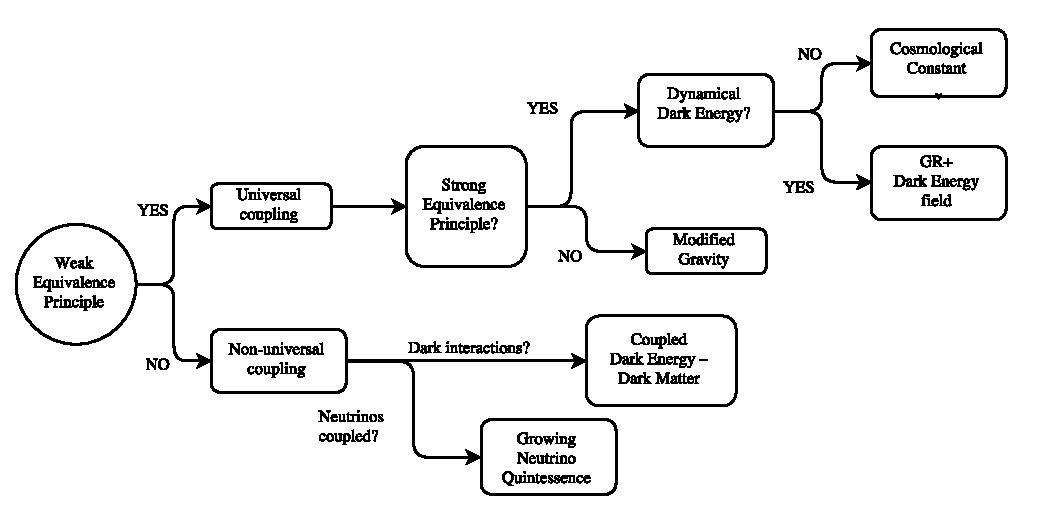
\includegraphics[width=0.99\textwidth]
		{Figures/DE-MG.pdf}
	\end{center}
	\caption[Dark Energy - Modified Gravity Flowchart]{Distinction between Dark Energy and
		Modified Gravity Theories based on the Strong and Weak Equivalence Principles (SEP and WEP), according to \cite{joyce_dark_2016-2}.
		The violation of the SEP, implies the existence of an extra fifth-force among particles, 
		or, equivalently, a modification of the standard Poisson equation. These are the so-called Modified Gravity theories.
		If the scalar degree of freedom is not coupled to matter, then we can talk about a Dark Energy model.
		In the case in which Dark Energy is not dynamical, the theory goes back to GR plus a cosmological constant.
		If the WEP is violated, then not all matter species feel the same gravitational forces and therefore
		there can be either dark sector interactions or neutrino--scalar-field interactions.
	}\label{fig:DE-vs-MG-WEP-SEP}
\end{figure}
%The term 
%Modified Gravity can encompass these but also other much more exotic modifications of GR, 
%for example involving extra dimensions and other 
%vector or tensor fields \cite{cite, bigravity, LH vector theory, dgp}. 
Furthermore, independent of the type of coupling to matter,
one can define two frames in which to study these theories. 
In the so-called Einstein frame, the action contains the standard Einstein-Hilbert term $R$,
plus a kinetic and a potential term for the scalar field $\phi$. 
However, particles are coupled to a metric that in principle depends also on the scalar field. 
On the other hand, in the Jordan frame, the scalar field $\varphi$ is non-minimally coupled
to gravity, which means that in place of the Ricci scalar,
there is a general function $f(R,\varphi)$. Besides, one can also have a potential
and kinetic term for the scalar field. 
The Einstein-Hilbert term is modified, but particles feel a metric that is purely of geometrical origin. 
We will specify the equations for these two different frames in
\cref{sec:Einstein-Jordan} below.
%but 
%One can regard this extra degree of freedom as an exotic new form of matter, affecting the right hand side of the Einstein field equation \ref{eq:Einstein-field-equations} and generally coupled in distinct ways to different matter fields, 
%or one can consider gravity to have an extra degree of freedom coupled non-minimally to the 
%Ricci scalar and therefore modifying 
%directly the left hand side of Einstein's field equations. The latter frame of reference
%is called the Jordan frame, while the former is usually called the Einstein frame.

%For theories in which all matter fields are coupled in the same way to the scalar field, both descriptions
%have to be equivalent and we call them \emph{universally coupled} theories. 
%For theories in which the coupling is specific to a matter field (i.e. neutrinos), the theory 
%is usually formulated in the Einstein frame. These are the so-called \emph{non-universally} coupled theories.
%In the following, we will use this classification to discuss the models studied in this work.

The distinction between Modified Gravity and Dark Energy is somewhat diffuse, since as mentioned above, 
an exotic form of matter in the Einstein's equations can always be considered as a modification 
of involving geometry. However, we will use a definition introduced recently by \cite{joyce_dark_2016-2}, 
which is quite practical in terms of its observable properties. 

In this definition, Dark Energy encompasses models which respect both the Weak and the Strong Equivalence
Principles and therefore do not involve extra fifth-forces that act between particles besides gravitational 
interactions (and the other three fundamental forces of nature). 
Modified Gravity encompasses models where the Strong Equivalence Principle is violated and therefore 
bodies can have an extra "scalar charge" that leads to the appearance of a fifth force among them.
In non-universally coupled theories, the Weak Equivalence Principle is violated,
since test bodies would feel different accelerations depending on
their composition. Usually, in these models baryons are uncoupled and therefore they might be called ``dark sector interaction`` theories.


The term ``modified gravity`` is also more general and it is used for
any theory beyond GR that is able to explain the cosmological history
of the Universe. This can include extra dimensions \cite{deffayet2002accelerated},
massive bimetric gravities \cite{akrami2015bimetric, konnig2014stable} or Lorentz-violating theories
\cite{blas2011models}. However, these models are out of the scope of this dissertation. 
For the rest of this work, when we mention Modified Gravity, we will refer to our definition according
to our discussion above and the diagram \ref{fig:DE-vs-MG-WEP-SEP}.

%In the first \cref{sec:universal-coupling} we will discuss universally coupled theories, which include ---among many others--- Quintessence, f(R),
%Scalar-Tensor theories and the Horndeski theory 
%(see \cite{Luca, Cliffton, Silvestri, Joyce, and more} for comprehensive reviews on Modified Gravity theories). 
%We will also discuss
%more general modifications of gravity which are based on the Effective Field Theory (EFT) approach to
%Dark Energy and parameterizations of modifications of gravity, which
%are not connected to any particular model and can accommodate any deviation from standard GR, at least at the linear 
%level in perturbation theory.
%
%In the second section, we will deal with two specific non-universally coupled models of dark energy used in this work. 
%The first one is
%called Coupled Dark Energy (CDE), which only couples the DE field to dark matter particles and leaves baryons uncoupled, therefore respecting solar system
%constraints on gravity.
%The second one, called Growing Neutrino Quintessence (GNQ), is a model in which the neutrino mass is coupled to the DE scalar field, while 
%all other species remain uncoupled, which is a very phenomenologically rich theory, but possesses theoretical difficulties due to its highly non-linear evolution.
%We will explain the motivations for each of these models and we will emphasize their differences in the predictions for structure formation and the background evolution of the Universe.
 
\section{The Einstein and the Jordan frames \label{sec:Einstein-Jordan}}

In this section we will review the form of the action for scalar-tensor theories in the Einstein and Jordan frames,
which are going to be useful concepts in the following chapters. For the moment we will work in units where the reduced Planck mass
$M_{Pl}^{2} = 1/(8 \pi G)$ is equal to unity.

A scalar-tensor theory can be formulated in the "Jordan frame" as:
\beeqalsp$\label{eq:jordan-frame-action}
\mathcal{S} =& \int \dx{4}{x} \sqrt{-g} \left[  \frac{1}{2} F(\varphi, R) - \frac{1}{2} K(\varphi) g^{\mu \nu}  \partial_{\mu}\varphi \partial_{\nu}\varphi 
- U(\varphi)    \right]  \\
& -\int \dx{4}{x} \sqrt{-g} \mathcal{L}^i_m (g_{\mu \nu} , \varPsi^i_m \zeta^{i}(\varphi)) \quad ,
$
where an index $i$ in the matter sector stands for each of the matter species in the Universe. 
In the case of universal coupling, all matter species ``feel`` the same metric $g$, 
 and are are coupled in the same way to the scalar field, through the function
 $\zeta^{i}(\varphi)$. 
In this frame, the Ricci scalar is non-minimally coupled to the field $\varphi$ through a function $F(R, \varphi)$ and, in general, 
can also contain a potential term for $\varphi$ with an extra function $K(\varphi)$ multiplying the kinetic term of the scalar field.
Matter particles follow the standard geodesics of GR and the energy momentum tensor of the matter species is covariantly conserved.

We can relate the Jordan to the Einstein frame, by doing a conformal transformation of the metric $g$, where
this transformation is defined as:
\beeqc$
\tilde{g}^{(i)} = \Omega^2(\phi, R) g
$
and $\Omega^2(\phi, R)$ is a function of the scalar field and ---in the most general case--- of the Ricci scalar, given by
\beeqp$
\Omega^2(\varphi,R) \equiv \parder{F}{R} 
$
Then, the scalar-tensor action in the `Einstein-frame` takes the following form:
\beeqc$\label{eq:einstein-frame-action}
\mathcal{S} = \int \dx{4}{x} \sqrt{-\tilde{g}} \left[  \frac{1}{2} \tilde{R} - \frac{1}{2} \tilde{g}^{\mu \nu}  \partial_{\mu}\phi \partial_{\nu}\phi 
- V(\phi)    \right] - \int \dx{4}{x} \sqrt{-\tilde{g}} \mathcal{L}^i_m (\tilde{g}^{(i)}_{\mu \nu} , 
\varPsi_m^{(i)} \tilde{\zeta}^{i}(\phi) )
$
where a tilde stands for the conformally transformed quantities.
In the case of universal coupling (see \cref{sec:universal-coupling} below), all matter species would couple to the same function $\tilde{\zeta}^{i}(\phi)$. 
If there is non-universal coupling (see \cref{sec:nonuniversal-coupling} below) each species would
have a different function $\tilde{\zeta}^{i}(\phi)$ or be totally uncoupled from the
field with $\tilde{\zeta}^{i}(\phi) = 1$. 
The Einstein frame is defined as the 
frame in which the gravitational part of the action looks standard, since the Ricci scalar appears without multiplicative factors.
In this formulation, the energy-momentum $T^{(m)}_{\mu \nu}$ of the coupled matter species is not conserved, but rather
the sum of the energy momentum tensor of matter and the scalar field $T^{(m+\phi)}_{\mu \nu}$ is the conserved quantity.

For non-relativistic particles this field dependent function $\zeta(\phi)$ can be also absorbed into the mass $m=m(\phi)$, giving rise to particles with varying mass, as we will see below.
This field dependent mass can also be linked to an extra "fifth-force", 
with a coupling strength $Q$
defined by:
\beeqc$\label{eq:definition-of-coupling-Q}
Q(\phi) \equiv -\frac{1}{2}\frac{\partial \ln f}{\partial \phi}
$
where, in these theories, the function $F$ above takes the form: $F(\varphi, R) = f(\varphi)R-2U(\varphi)$, where
$f$ and $U$ are free functions of the field.
To go from the Jordan frame action \cref{eq:jordan-frame-action} to the Einstein frame action
\cref{eq:einstein-frame-action} and at the same time keep a \emph{canonical} kinetic term,
($1/2 \nabla^2 \phi$), a field redefinition has to be performed:
\beeq$
\phi = \int \dx{}{\varphi} \sqrt{(3/2)(f_{,\varphi}/f)^2 + K/f}
$
where the potentials $U$ and $V$ are related by $V = U/f^2$.


For non-universal coupling, we will see two examples of theories formulated in the Einstein frame in \cref{sub:CDE} and \cref{sub:GNQ}.
In \cref{sub:CDE} we will see an example of a constant coupling and in \cref{sub:GNQ} we will see an example of a field-dependent coupling, 
giving rise to very different phenomenologies.

For conformally-invariant theories (those theories in which null-geodesics are not modified by conformal transformations), the conformal factor
just depends on the scalar field and can be written as $\Omega^2(\varphi)=\exp(2\varphi)$. 
This can be seen by performing the transformation $g \rightarrow e^{2\varphi} g$ and 
observing that, at first order in the
scalar field and the gravitational potentials, $\Phi \rightarrow \Phi-\varphi$ and $\Psi \rightarrow \Psi+\varphi$, leaving 
the Weyl (lensing) potential $\Phi_{\rm Weyl} = (1/2)(\Psi + \Phi)$ invariant.
These theories are interesting, since they do not affect gravitational lensing observations,
but still can provide interesting non-standard features in the clustering of matter.


We have to emphasize that physical measurable quantities have to be frame-independent by definition,
since this frame transformation amounts to nothing more than a coordinate and field redefinition 
and one of the principles of the GR formalism which we are not abandoning
is diffeomorphism invariance, which ensures that 
the theory is invariant under general coordinate transformations.


\section{Universal coupling to matter \label{sec:universal-coupling}}

Scalar-tensor theories with universal coupling written in the Jordan frame \cref{eq:jordan-frame-action}, 
encompass many of the most widely studied dark energy and modified gravity models in the literature. 
For example, $f(R)$ theories \cite{de2010f} are recovered when $F(R,\varphi) = f(R)$ and $K=0$;
Brans-Dicke theory \cite{brans1961mach} is recovered when $F(R,\varphi) = \varphi R $ and 
$K(\varphi) = \omega_{BD}/\varphi$, where $\omega_{BD}$ is the Brans-Dicke parameter and finally "k-essence" 
\cite{armendariz2001essentials} is the case in which $F(R,\varphi) = R$ and $K$ can be a general
function of $\varphi$ and its kinetic term $(\nabla \varphi)^2$. 

There are also other theories of modified gravity with a scalar field, that are not encompassed in the set of "scalar-tensor"
theories and that have gained a lot of attention recently. Namely, Galileons \cite{deffayet2011k}, Horndeski \cite{deffayet2013formal} 
and Beyond-Horndeski theories \cite{gleyzes2015exploring}. 
These theories are universally coupled to matter, are formulated
in the Jordan frame and cannot be expressed in the Einstein frame by a conformal transformation, since they contain much more complicated
derivative interactions, for example free functions of $\Box \varphi$ (see \cite{zumalacarregui2014transforming}), where the ``box operator`` is defined as $\Box \equiv g^{\munu}\partial_{\mu}\partial_{\nu}$.

Horndeski's theory \cite{horndeski_original} is an interesting case, since it is the most general theory of 
a scalar field coupled to a metric, with second order equations of motion and free of ghost instabilities. 
This theory was first formulated by Horndeski in the 1970's \cite{horndeski_original}, in a purely mathematical way and was re-discovered by \cite{deffayet2013formal}
and others, at the beginning of the present decade, in the context of Galileon scalar fields. The simplest Galileon model, the so-called cubic Galileon, has a Lagrangian of the form:
$\mathcal{L} \propto R/2 - (\partial \varphi)^2 - (1/\Lambda_3)\Box \varphi (\partial \varphi)^2$, 
where $ \Lambda_3 $ is a free scale that can be set in the theory. The term Galileons, comes from the fact that
these theories are the more general theories, which are invariant under a general Galiliean transformation of the field $\varphi \rightarrow \varphi + b_\mu x^\mu +c$.
Beyond-Horndeski theories are extensions of Horndeski that have higher than second order equations of motion, when expressed 
in the Newtonian gauge, but where the propagating scalar degree of freedom still obeys second order differential equations, avoiding
instabilities, see
\cite{gleyzes2015exploring} and \cite{zumalacarregui2014transforming} for more details on this direction of research.

For the purposes of this work, we will now detail one of the oldest models of Dark Energy, namely
the Quintessence model \cite{ratra_cosmological_1988, wetterich_cosmology_1988} and its extension
Coupled Quintessence introduced by \cite{Amendola_2000}.

Later on we will deal with general modifications of gravity, whose
effect on structure formation can be parameterized by two functions of
scale and time. Finally we will shortly explain one of the most general approaches
to construct theories of modified gravity at linear order; the so-called Effective Field Theory of Dark Energy. We will show also its connection to Horndeski's theory.

\subsection{Quintessence \label{sub:quintessence}}

The Quintessence model
%, which takes its name from the Latin word for "fifth element"
%is one of the oldest models of Dark Energy. It 
was introduced by several authors almost 30 years
ago \cite{ratra_cosmological_1988, wetterich_cosmology_1988},
motivated by studying the 
breaking of scale invariance, which could give rise to a dynamical cosmological constant.
Its Lagrangian is of the form \cref{eq:jordan-frame-action}, with
$F(\varphi, R) = R$, $K = 1$ and a potential $U(\varphi)$.
Since this is a homogeneous field without couplings, we can find its energy density and its pressure 
straightforwardly from the energy-momentum tensor of a perfect fluid in a FLRW background:
\begin{align}\label{eq:quintessence-rho-p}
&\rho_{\varphi} = -T^{0 (\varphi)}_0 = \frac{1}{2}\dot\varphi^2 + U(\varphi) \quad 
&p_{\varphi} = \frac{1}{3} T^{i (\varphi)}_i = \frac{1}{2}\dot\varphi^2 - U(\varphi) \quad ,
\end{align}
which yields the equation of state:
\beeqp$
w_\varphi  = \frac{p_{\varphi}}\rho_{\varphi} = \frac{\dot\varphi^2 - U(\varphi)}{\dot\varphi^2 + U(\varphi)}
$
We can see that for obtaining the required behavior of $w\approx -1$ at late times, in order to fit 
the observations of the expansion of the Universe, we need that the kinetic term $\dot\varphi^2$
becomes much smaller than the potential term $U$.
From the continuity equation for a perfect fluid or from the variation of the action with respect to $\varphi$,
we can find the Klein-Gordon equation for this field:
\beeqp$
\label{eq:Klein-Gordon-Quintessence}
\ddot \varphi + 3 H \dot \varphi + U_{,\varphi} = 0
$
The dynamics and the phenomenology of this model are entirely determined by the shape of the potential
and for this there are many possibilities (see \cite[chap. 7]{amendola_dark_2010}, for a comprehensive review).
The most interesting solutions, which can alleviate the cosmological coincidence problem, are those in which the field
tracks the evolution of matter at early times ($w_\varphi \approx 1$) and then 
evolves towards an attractor (effectively being independent of initial conditions) 
at late times, which yields cosmic acceleration with $w_\varphi \approx -1+\xi$.
The parameter $\xi$ is a combination of parameters entering the potential function $U(\varphi)$ and allows
to distinguish Quintessence from a simple cosmological constant at present time.
The most studied potentials are the exponential potential $U(\varphi) = U_0\exp(-\lambda \varphi)$ 
(see \cite{copeland_exponential_1998}), where $\lambda$ is a free parameter
and the inverse power-law potential $U(\varphi) = M^{4+n} \varphi^{-n}$,
where $M$ is a mass scale of the theory.

Due to the so low energy density of dark energy ($\rho_{DE} \approx 10 ^{-120} M_{Pl}$)
compared to typical energies appearing in particle physics, it is not so easy to construct a 
viable model of Quintessence which is motivated by a fundamental theory. Nevertheless, there are 
some succesful approaches like fermion condensates, Pseudo-Nambu-Goldstone models and 
dilatonic quintessence (see \cite{amendola_dark_2010} and references therein).
These models have to satisfy that at present times dark energy is the dominating 
energy density in the Universe and therefore from the Friedmann equation and \cref{eq:quintessence-rho-p}:
\beeqp$
U(\varphi_0) \approx H_0^2 M_{Pl}^2
$
If we take an inverse power law potential, $U(\varphi) = M^{4+n} \varphi^{-n}$, and take the field to be at present $\varphi_0 = M_{Pl}$,
this would yield a mass scale $M$ of the order
of:
\beeqc$
M \approx H_0^{2/(4+n)} M_{Pl}^{(2+n)/(4+n)}
$
where, with $H_0 \approx 10^{-42} \mathrm{GeV} $, we get a mass scale of $M \approx 10^{-1} \mathrm{GeV}$
for $n=2$, which is a scale compatible with Standard Model particles.
Moreover, to satisfy the requirement of acceleration today, 
the slow-roll condition (analogous to the one in inflation \cite{bartolo_non-gaussianity_2004}) must satisfy 
$ \frac{M_{Pl} V_{,\varphi \varphi}}{V(\varphi_0)} \lessapprox 1$.
Defining the mass of the scalar field $m_\varphi$ as the second derivative of the potential with respect to the field,
$m^2_\varphi \equiv  V_{,\varphi \varphi} $, yields a condition for the scalar field mass:
\beeqp$
m_\varphi \lessapprox H_0 \approx 10^{-33} \mathrm{eV}
$
So in order to be compatible with observations, 
the scalar field mass must be extremely small.
This could cause problems for quintessence models,
since the stability of such small masses is not always guaranteed under radiative corrections \cite{kolda1999quintessential}.

\subsection{Coupled Quintessence \label{sub:CQ}}

It is also interesting to observe the effects of a coupling between the 
scalar field and the matter species.
In \cref{eq:definition-of-coupling-Q} we already saw how from a general
Scalar-Tensor theory, a coupling between matter species and 
the field can arise from an action like the one in \cref{eq:jordan-frame-action}.
However, the matter equations of motion and the Klein-Gordon equation become more tractable if
we make a conformal transformation into the Einstein frame, where
the scalar field Lagrangian will be canonical, but matter will
be coupled to a metric that contains a function of the field $\phi$.
In this case, as stated before, the individual energy-momentum tensors will not
be conserved:
\beeqal$\label{eq:Tmunu-for-CQ}
&\nabla_{\mu} T^\mu_{\nu (\phi)} = -Q T_m \nabla_{\nu}\phi \quad & \nabla_{\mu} T^\mu_{\nu (m)} = +Q T_m \nabla_{\nu}\phi \;\;,
$
where $Q$ is the coupling function and $T_m$ the trace of the energy-momentum tensor of matter. Through the 
conformal transformation the field should also be coupled to radiation, since radiation also feels gravity, 
but since the trace of the energy-momentum tensor of radiation vanishes identically, it does not appear in the 
conservation equations.
In general,
the coupling $Q$ can be different for baryons and for dark matter.
The coupling to baryons is severely constrained by local gravity experiments (see \cite{Agashe:2014kda})
and therefore uncoupling the baryons from the theory 
can yield a model compatible with observations as we will see below for the Coupled Dark Energy model in \cref{sub:CDE}.

If all matter fields are coupled, then some screening mechanism
has to be invoked in order to pass the stringent Solar System and local gravity constraints.
One possibility is the chameleon mechanism (see the book by \citetitle{amendola_dark_2010}, for a comprehensive review), which
is a coupled quintessence field whose effective potential (and therefore its effective mass)
changes according to the environment it is in.
These kind of theories can arise from an action like in \cref{eq:jordan-frame-action},
with $F(\varphi,R) = \exp(-2Q\varphi)R$ and $K(\varphi) =(1-6Q^2)\exp(-2Q\varphi)R$.
For each distribution of matter, taken to be spherically symmetric for simplicity, 
one has to calculate the profile of the field $\varphi (r)$ as a function of the radius $r$,
and one can tune the parameters in such a way that the effective coupling $Q_{\rm eff}$
in a certain region is much smaller than the bare coupling $Q$ appearing in the action.
In this way one can recover for star systems and galaxies the Newtonian predictions.
For more details on these calculations, see \cite{amendola_dark_2010}, chapter 8.4.



\subsection{Effective Field Theory of Dark Energy and Horndeski Theory \label{sub:EFT-of-DE}}

Until now we have treated Dark Energy and Modified Gravity in a rather phenomenological way,
adding a scalar field with an kinetic term, a coupling and a potential without a clear understanding
of which terms are allowed or not.
Recently, there have been substantial efforts by many authors to build an effective field theory 
of dark energy and modified gravity that encompasses all possible terms that are allowed 
in the action at second order (see \cite{Gubitosi2013, Gleyzes2016, bloomfield_dark_2013}). Considering only one extra dynamical
scalar field, respecting the symmetries of homogeneity and isotropy and following the Weak Equivalence Principle (WEP),
this theory can be uniquely formulated. Its action in the Jordan frame (and written in conformal time $\tau$) takes the form:
\begin{align}\label{eq:EFT-action}
\begin{split}
S ={}& \int \dx{4}{x} \sqrt{-g} \left[ \frac{M_{Pl}^2}{2} [1 + \Omega(\tau)] R + \Lambda(\tau) -a^2 c(\tau)\delta g^{00} \right. \\
     & + \frac{M_{2}^4 (\tau)}{2}(a^2 \delta g^{00})^2 -\bar{M}_{1}^3 (\tau) 2 a^2 \delta K^\mu_\mu \delta g^{00} \\
     & - \frac{\bar{M}_2^2 (\tau)}{2} (\delta K_\mu^\mu )^2 - \frac{\bar{M}_3^2 (\tau)}{2}\delta K^{\mu}_{\nu}\delta K^{\nu}_{\mu} \\
     & + a^2 \frac{\hat{M}^2 (\tau)}{2} \delta g^{00} \delta R^{(3)} \\
     & + m^2_2(\tau) (g^{\mu \nu} + n^\mu n^\nu) \partial_{\mu} (a^2 g^{00})\partial_{\nu} (a^2 g^{00}) \\
     & \left. + \mathcal{L}_m(g_{\mu \nu}, \varPsi_m) \right] \quad.
\end{split}
\end{align}
To construct this action, the spacetime has been foliated (similarly to the 3+1 ADM decomposition) into a time direction
and spatial hypersurfaces that coincide with the uniform scalar field hypersurfaces (this is the so-called unitary gauge). 
The preferred time direction is then (c.f. \cite{Gubitosi2013})
\beeqc$
n_\mu \equiv -\frac{\partial_{\mu}\phi}{\sqrt{-(\partial \phi)^2}}
$
which induces a spatial metric $h_{\mu \nu} \equiv g^{\mu \nu} + n^\mu n^\nu $, a spatial Ricci scalar $R^{(3)}$
and defines an extrinsic curvature:
\beeqp$
K_{\mu \nu} \equiv h^{\sigma}_{\mu} \nabla_{\sigma} n_\nu
$
The rest of the terms in the EFT action \cref{eq:EFT-action} are nine free functions of time:\\
$\{\Omega(\tau), \Lambda(\tau), c(\tau), M_{2}^4 (\tau), \bar{M}_{1}^3 (\tau), \bar{M}_2^2 (\tau), \bar{M}_3^2 (\tau),
 \hat{M}^2 (\tau), m^2_2(\tau)\}$, whose choice specify the theory.
This theory encompasses all theories of an extra dynamical scalar field, which respect the WEP.
At the linear level in perturbations, it includes the Horndeski theory (mentioned above in \cref{sec:universal-coupling}) 
and also theories which go beyond second order equations of motion (in the Newtonian gauge), also called
Beyond-Horndeski theories (see \cite{gleyzes2015exploring})

Since these theory involves many free functions, we need to choose a parametrization for each of them and 
we need to take some simplifying assumptions in order to be able to constrain this theory with data.
Recently, a code capable of calculating the linear Einstein-Boltzmann system of equations for the EFT formalism
has been made public, the so-called \textsc{EFTCAMB} (\cite{hu_effective_2014, hu_eftcamb/eftcosmomc:_2014-2}), which is based 
on the widely used \textsc{CAMB} code by\cite{lewis_efficient_2000}. 
We will use this code to calculate the observables which we will 
implement into our Fisher forecast in \cref{sec:EFT-forecasts}.

Furthermore, we will use the assumptions taken in \cite{planck_collaboration_planck_2016} in order to simplify
the theoretical modeling.
If we assume a $\lcdm$ background, and choose freely a function
$\Omega(\tau)$, the functions $\Lambda(\tau) \textrm{ and } c(\tau)$ are then fixed \cite{hu_effective_2014}.
Furthermore, we will impose $ m^2_2(\tau) = 0$ and $ \bar{M}_2^2 (\tau) = - \bar{M}_3^2 (\tau)$,
which eliminates models which contain third-order spatial derivatives.
Now we just have 5 free functions of time and a function specifying the background cosmology $H(\tau)$.
These free functions of time can be mapped to the Bellini-Sawicki $\alpha_i (\tau)$ 
functions (see \cite{bellini_maximal_2014}),
which fully specify the evolution of Horndeski models at linear order in perturbation theory. The following relations between the EFT functions and the $\alpha$ functions hold:
\beeqal$ \label{eq:EFT-funcs}
\begin{split}
M_{*}^2 (\tau) & = M_{Pl}\Omega(\tau) + \bar{M}_2^2 (\tau) \\
M_{*}^2 (\tau) H(\tau) \alpha_M (\tau)   & = M_{Pl}\dot{\Omega}(\tau) + \dot{\bar{M}}_2^2 (\tau) \\
M_{*}^2 (\tau) H^2(\tau) \alpha_K (\tau)   & = 2 c (\tau) + M_2^4 (\tau) \\
M_{*}^2 (\tau) H(\tau) \alpha_B (\tau)   & = M_{Pl}\dot{\Omega}(\tau) - \bar{M}_{1}^3 (\tau)\\
M_{*}^2 (\tau) \alpha_T (\tau)   & = - \bar{M}_2^2 (\tau) \\
M_{*}^2 (\tau) \alpha_H (\tau)   & = 2 \hat{M}^2(\tau) - \bar{M}_2^2 (\tau)
\end{split}
$ 
Here, the bare reduced Planck mass is $M_{Pl}$ and the effective Planck mass is $ M_{*}^2 $.
These $\alpha_i$ functions are much easier to interpret physically than the EFT functions.

The first four $\alpha_i$ functions, $\alpha_M$, $\alpha_K$,
$\alpha_B$ and $\alpha_T$  describe fully the physics
of linear perturbations in Horndeski's theory (see \cite{bellini_maximal_2014}).
For instance, $\alpha_M$ (\emph{mass run rate}) is the rate of change of the effective Planck mass, 
produces anisotropic stress; $\alpha_K$ (\emph{kineticity}) is present in Quintessence (\cref{sub:quintessence}) models, 
but also in models where the scalar field has a non-zero sound speed, like k-essence models;
$\alpha_B$ (\emph{braiding}) causes dark energy to cluster and $\alpha_T$ is the \emph{tensor speed excess}, which gives the deviation
of the speed of gravitational waves from that of light.
Finally $\alpha_H$ is a term indicating physics that lies beyond the Horndeski models at linear level. 
For our results in \cref{sec:EFT-forecasts}, we will further reduce this theory to a simpler case, 
which can be compared easier with Large-Scale-Structure observations.


\subsection{Parameterizing Modified Gravity \label{sub:parameterizing-MG}}

In the previous sections we have seen how to construct Dark Energy and Modified Gravity theories 
which have an extra scalar degree of freedom, besides the Einstein-Hilbert term and the matter and radiation species.
As we have seen, one can successfully construct the most general theory of this kind, by either imposing
some conditions on the equations of motion and the stability of the theory (as in Horndeski theories) or by considering all
possible terms allowed by symmetries in the second order action (as in EFT).

However, for observations, these general theories are not so practical, since there is not enough data to constrain
all the free functions in the Lagrangian. What we really can observe with Galaxy Clustering and Weak Lensing 
are the perturbations of matter $\delta_m(z,k)$, its correlation function across scales $P_m(z,k)$ and the
evolution of matter structures in time, $f(z)$.
In Einstein-GR, these three quantities are determined by the gravitational potentials $\Phi$ and $\Psi$, which follow 
the general relativistic Poisson equations (see \cref{eq:relativistic-Poisson}). 
In linear perturbation theory, scalar, vector and tensor perturbations
do not mix, which allows us to consider only the scalar perturbations of the metric. 
We work in the conformal Newtonian gauge, with the
line element given by \cref{eq:linearized-metric-scalar}
%\begin{equation}
%ds^{2}=-(1+2\Psi)dt^{2}+a^{2}(1-2\Phi)dx^{2}\,\,\,.
%\end{equation}
The potentials $\Phi$ and $\Psi$ are in functions of time and in our notation, they coincide
with the gauge-invariant Bardeen potentials.

%In modified gravity, it has been shown that
%the deviations from Einstein-GR can be fully described by 
%two generic free functions of time and space \cite{kunz_phenomenological_2012, amendola_observables_2013}.
%While any two (independent) functions of the gravitational potentials would be suitable, 
%we consider in this work the most common parameterization (see \cite{planck_collaboration_planck_2016}) given by $\mu(a,k)$ and $\eta(a,k)$: the first modifies the Poisson equation for $\Psi$ while the second is equal to the ratio of the gravitational potentials and is therefore also a direct observable \cite{amendola_observables_2013}.

%In section \ref{sec:Parameterizing-Modified-Gravity} we define $\mu$ and $\eta$ and parameterize them in three different ways. First, in a general manner, we let these functions vary freely in different  redshift bins. Complementarily, we also consider two specific parameterizations of the time evolution proposed in \cite{planck_collaboration_planck_2016}. Here, we also specify the fiducial values of our cosmology for each of the
%parameterizations considered.

In theories with an extra scalar degree of freedom (see the discussion around \cref{fig:DE-vs-MG-WEP-SEP} for a distinction between Dark Energy and Modified Gravity)
the standard linear perturbation equations
are no longer valid, so that for a given matter source the values
of $\Phi$ and $\Psi$ will differ from their Einstein-GR values (see \cite{kunz_phenomenological_2012, amendola_observables_2013}). We can
parameterize this change generally with the help of two new functions $\mu(a,k)$ and $\eta(a,k)$
that encode the modifications. Many different choices are possible
and have been adopted in the literature, see e.g. \cite{planck_collaboration_planck_2016} for a limited overview. 
In this work
we introduce the two functions through a gravitational slip (leading
to $\Phi\neq\Psi$ also at linear order and for pure cold dark matter)
and as a modification of the Poisson equation for $\Psi$, 
\begin{align}
-k^{2}\Psi(a,k) & \equiv  4\pi
Ga^{2}\mu(a,k)\rho(a)\Delta(a,k)\,\,\,;\label{eq:mu_def}\\
\eta(a,k) & \equiv \Phi(a,k)/\Psi(a,k) \quad \label{eq:eta_def}.
\end{align}
These expressions define the modified gravity functions
$\mu$ and $\eta$. Here $\rho(a)$ is the average dark matter density and $\delta(a,k)$
the comoving matter density contrast -- we will neglect relativistic
particles and radiation as we are only interested in modeling the
perturbation behaviour at late times. 
In this formulation, $\eta$,
which is effectively an observable \cite{amendola_observables_2013}, is closely related to
modifications of GR \cite{saltas_anisotropic_2014,sawicki_non-standard_2016}, 
while $\mu$ encodes for example deviations in
gravitational clustering, as non-relativistic particles are accelerated by the gradient of $\Psi$.

When considering Weak Lensing observations then it is also natural
to parameterize deviations in the lensing or Weyl potential $\Phi+\Psi$,
since it is this combination that affects null-geodesics.
To this end we introduce a function $\Sigma(a,k)$ so that
\begin{equation}\label{eq:Sigma-def}
-k^{2}(\Phi(a,k)+\Psi(a,k))\equiv8\pi
Ga^{2}\Sigma(a,k)\rho(a)\delta(a,k) \quad .
\end{equation}
Since metric perturbations are fully specified by two functions of
time and scale, $\Sigma$ is not independent from $\mu$ and $\eta$,
and can be obtained from the latter as follows: 
\begin{equation}\label{eq:SigmaofMuEta}
\Sigma(a,k)=(\mu(a,k)/2)(1+\eta(a,k)) \quad.
\end{equation}
Throughout this work, we will denote the standard Lambda-Cold-Dark-Matter ($\Lambda$CDM) model,
defined through the Einstein-Hilbert action with a cosmological constant, simply as Einstein-GR, where $\mu=\eta=\Sigma=1$. 
If only $\mu$ deviates from unity at late times,
it indicates either Modified Gravity or just a Dark Energy field that clusters.
If $\eta$ deviates from unity, it is an indication for Modified Gravity models, according to our definitions above \cref{fig:DE-vs-MG-WEP-SEP}, based on \cite{joyce_dark_2016}.


Using effective quantities like $\mu$ and $\eta$ has the advantage
that they are able to model {\em any} deviations of the perturbation
behaviour from $\Lambda$CDM expectations, they are relatively close 
to observations, and they can also be related to other commonly used 
parameterizations \cite{pogosian_how_2010}.
On the other hand, they are not
easy to map to an action ---as opposed to approaches like Effective
Field Theory (EFT, \cref{sub:EFT-of-DE})---  and in addition they
contain so much freedom that we normally restrict their parameterization
to a subset of possible functions.


\subsubsection{Parameterizing gravitational potentials with simple smooth functions of the scale factor \label{sub:param-smooth-funct}}

The first possibility is to assume simple specific time parameterizations for
the $\mu$ and $\eta$ functions, adopting the ones used in the
\planck\ analysis \cite{planck_collaboration_planck_2016}, where we neglect here any scale dependence:
\begin{itemize}
	\item a parameterization in which the time evolution is related to the dark
	energy density fraction, to which we refer as `late-time' parameterization:
	\beeqal$
	\mu(a,k) \equiv& \; 1+E_{{\rm 11}}\Omega_{{\rm
			DE}}(a)  \quad ,\label{eq:DE-mu-parametrization}\\
	\eta(a,k)\equiv& \; 1+E_{{\rm 22}}\Omega_{{\rm
			DE}}(a)  \quad ;\label{eq:DE-eta-parametrization}
     $
	
	\item a parameterization in which the time evolution is the simplest first
	order Taylor expansion of a general function of the scale factor $a$
	(and closely resembles the $w_{0}-w_{a}$ parametrization for the
	equation of state of DE), referred to as `early-time' parameterization, because it
	allows departures from GR also at high redshifts:
%	\footnote{Notice that our early-time parametrization is called
%		`time-related' in \cite{planck_collaboration_planck_2016}.}:
	\beeqal$
	\mu(a,k)\equiv & \; 1+E_{{\rm 11}}+E_{{\rm
			12}}(1-a)  \quad,\label{eq:TR-mu-parametrization}\\
	\eta(a,k)\equiv & \; 1+E_{{\rm 21}}+E_{{\rm
			22}}(1-a)  \quad.\label{eq:TR-eta-parametrization}
	$	
\end{itemize}
The parameters $E_{i j}$ are usually order-unity parameters, which give the amplitude of the modifications
at present time: $E_{11}$ for $\mu$ and $E_{22}$ for $\eta$ in the late-time parameterization and 
$E_{11}$ for $\mu$ and $E_{21}$ for $\eta$ in the early-time parameterization, while
$E_{12}$ and $E_{22}$ measure the slope of the time-evolution function.


The late-time parameterization is forced to behave as Einstein-GR ($\mu=\eta=1$)
at high redshift when $\Omega_{{\rm DE}}(a)$ becomes negligible;
the early time parameterization allows more freedom as the amplitude of the deviations
from Einstein-GR do not necessarily reduce to zero at high redshifts. 
Both parameterizations have been used in \cite{planck_collaboration_planck_2016}
and in other recent studies of how to constrain Modified Gravity with Galaxy Clustering and Weak Lensing observations, see
\cite{bull_extending_2015, Gleyzes2016} and \cite{Alonso2016}.
In \cref{chap:MG-forecasts} we will study in more detail both the late-time and the early-time parameterizations and we will
try to find out how well future observations will be able to measure $\mu$ and $\eta$, using linear and non-linear
matter perturbations.


\subsubsection{Parameterizing gravitational potentials in discrete redshift bins \label{sub:param-z-bins-th}}

A second and more model-independent approach
is to specify the time evolution of the functions $\mu$ and $\eta$ without
any parameterization.
To this purpose we "pixelize" the functions $\mu$ and $\eta$ at $N$ redshift bins $z_i$, with $i=\{1, \ldots N  \}$ 
and we consider the values
$\mu(z_{i})$ and $\eta(z_{i})$ at the right limiting redshift $z_{i}$
of each bin as free parameters.
The $\mu(z)$ function (and analogously $\eta(z)$) is then reconstructed
as 
\begin{equation}\label{eq:MGbin-mu-general-parametrization}
\mu(z)=\mu(z_{1})+\sum_{i=1}^{N-1}{\frac{\mu(z_{i+1})-\mu(z_{i})}{2}\left[1+\tanh{\left(s\frac{z-z_{i+1}}{z_{i+1}-z_{i}}\right)}\right]},
\end{equation}
where $s=10$ is a smoothing parameter and $N$ is the number of binned
values. We assume that both $\mu$ and $\eta$ reach the Einstein-GR limit
for a redshift higher than $z_h$: to realize this, the last $\mu(z_{N})$ and $\eta(z_{N})$
values assume the standard $\lcdm$ value $\mu=\eta=1$ and both functions
are kept constant at higher redshifts $z> z_h$.


Similarly, the derivatives of these functions are obtained by computing
\begin{equation}
\mu'({\bar{z}_{j}})=\frac{\mu(z_{i+1})-\mu(z_{i})}{z_{i+1}-z_{i}},
\end{equation}
with $\bar{z}_{j}=(z_{i+1}+z_{i})/2$, using the same $\tanh(x)$
smoothing function: 
\begin{equation}\label{eq:MGbin-muderiv-parametrization}
\frac{d\mu(z)}{dz}=\mu'(\bar{z}_{1})+\sum_{j=1}^{N-2}{\frac{\mu'(\bar{z}_{j+1})-\mu'(\bar{z}_{j})}{2}\left[1+\tanh{\left(s\frac{z-\bar{z}_{j+1}}{\bar{z}_{j+1}-\bar{z}_{j}}\right)}\right]}\,\,\,.
\end{equation}
In particular we assume $\mu'=\eta'=0$ for $z<0.5$ and for $z>3$.

This approach has the advantage of being independent of the parameterization of the time evolution of $\mu$ and $\eta$,
but at the cost of introducing
many more parameters that have to be constrained by observations.
Furthermore, one does not know a priori how many binned parameters have to be taken into account
and what are the degeneracies among them.
This will be the subject of study in \cref{chap:MG-forecasts}, where we will
introduce the functions $\mu$ and $\eta$ parameterized in redshift bins and we will forecast
how well future observations will be able to measure those functions.



\section{Non-universal coupling \label{sec:nonuniversal-coupling}}

In \cref{sec:DE-MG-sec} we have motivated the inclusion of a scalar field as a 
way of solving the dark energy problem and alleviating the coincidence problem.
The energy fraction of Dark Energy and that of Dark Matter are of the same
order of magnitude only for a very short period of time in cosmological time scales and that time is precisely
now when we are capable of making observations. This introduces the question if this is just a coincidence or 
if somehow Dark Energy and Dark Matter are connected beyond simple gravitational physics.
Therefore a natural way of alleviating this "coincidence problem" issue (which we discussed in \cref{sub:CC-problem})
is to imagine there is a coupling in the dark sector or some mechanism that connects the onset of non-linear 
structure formation to the epoch of accelerated expansion of the Universe. As we will see, the coupling to baryons 
is extremely well constrained by solar system and galactic observations and therefore a coupling to baryons 
has to be avoided.

In this section we will deal with two non-universally coupled theories which can yield very distinctive 
effects on the formation and evolution of structures in the Universe.
In the first model, called (\cref{sub:CDE}) Coupled Dark Energy, there exists an exchange of energy and momentum
between a quintessence scalar field and the dark matter particles. 
The second one is also a quintessence model, but this time the masses of neutrinos are 
coupled to the scalar field. In this model, the DE domination is triggered by the neutrinos becoming non-relativistic
and their mass is connected to the energy scale attributed to the DE field.

As we have seen before, if the Weak Equivalence principle is violated, then there exists a fifth force acting between test
particles on top of the gravitational interaction. Generally this will yield modifications in the growth rate of perturbations, 
the density profiles of structures and the matter power spectrum. Since the effects appear generally the non-linear regime,
we will have to study them by performing numerically expensive N-body simulations, as we will see in \cref{chap:Fitting-CDE}
and \cref{chap:GNQ}.


\subsection{Coupled Dark Energy \label{sub:CDE}}

We explained in \cref{sub:CQ} how a coupling between all matter species and a scalar field can be realized in the Jordan frame.
However, for non-universal couplings it is easier to work in the Einstein frame, in which the Lagrangian takes the form:
\beeqalsp$\label{eq:CDE-Lagrangian}
\mathcal{L} = \frac{1}{2} \tilde R - \frac{1}{2} \tilde{g}^{\mu \nu}  \partial_{\mu}\phi \partial_{\nu}\phi 
- V(\phi) - m(\phi) \bar{\psi} \psi + \mathcal{L}_{\rm kin}(\psi) \quad,
$
where $\psi$ is the coupled dark matter field, $m$ its mass and $\mathcal{L}_{\rm kin}(\psi)$
its kinetic term.

The coupling to baryons is severely constrained by observations at solar system scales.
The ``post-Einstein'' coupling parameter $\bar{\gamma}$ defined as the quantity that
measures the local admixture of a scalar field to gravity is
constrained in Solar System experiments  roughly to
$|\bar{\gamma}|\le4\cdot10^{-5}$ (see e.g. the PDG review \cite{Agashe:2014kda}
and \citep{Will_2005,Bertotti_Iess_Tortora_2003}). 
This parameter enters the modification
of the effective Newton constant as $G_{eff}=G_{N}(1-\bar{\gamma}/2)$. 
We will see below, that the effective force coming from a coupling to matter is
in our notation, $G_{eff}=G_{N}(1+4\beta^{2}/3)$
and therefore $\beta^{2}=-3\bar{\gamma}/8$. A coupling $\beta_{\rm baryons}^{2}$
appears then constrained to be smaller than $10^{-5}$ roughly, and
we assume therefore that is completely negligible. As a consequence,
baryons follow the usual geodesics of a FLRW cosmology, which allows
coupled DE to pass the stringent local gravity constraints without 
the need to employ any screening mechanism \cite{hamilton_atom-interferometry_2015}, 
\cite{khoury2010theories, bloomfield2015shape}.

The background evolution for the coupled DE scenario model is described
by the following equations, in which the subscripts $r$, $b$, $c$
and $\phi$, indicate radiation, baryons, cold dark matter (CDM) and
the dark energy scalar field, respectively:

\begin{eqnarray}
\ddot{\phi}+3H\dot{\phi}+\frac{dV}{d\phi} & = & \sqrt{\frac{2}{3}}\beta(\phi)\frac{\rho_{c}}{M_{Pl}}\,\,,\label{eq:quint-kleingordon}\\
\dot{\rho}_{c}+3H\rho_{c} & = & -\sqrt{\frac{2}{3}}\beta(\phi)\frac{\rho_{c}\dot{\phi}}{M_{Pl}}\,\,,\label{eq:cdm-back-density}\\
\dot{\rho}_{b}+3H\rho_{b} & = & 0\,\,,\\
\dot{\rho}_{r}+4H\rho_{r} & = & 0\,\,,\\
3H^{2} & = & \frac{1}{M_{Pl}^{2}}(\rho_{b}+\rho_{c}+\rho_{r}+\rho_{\phi})\,\,.
\end{eqnarray}


We express the scalar field $\phi$ in units of the Planck
mass $M_{pl}\equiv1/\sqrt{8\pi G}$, and choose as potential $V(\phi)$
an exponential $V(\phi)=Ae^{-\alpha\phi}$ \citep{Lucchin_Matarrese_1984,Wetterich_1988}.
The coupling function $\beta(\phi)$ defines the strength of the interaction
between the DE fluid and CDM particles and in the present work we
will restrict our analysis to the simplified case of a constant coupling
$\beta(\phi)=\beta$, although in general it could be a field-dependent
quantity \cite{Amendola_2004,Baldi_2011a}.

Due to the exchange of energy between DE and CDM, the energy density
of the latter will no longer scale as the cosmic volume, and by assuming
the conservation of the CDM particle number one can derive the time
evolution of the CDM particle mass by integrating Eq.(\ref{eq:cdm-back-density})
between the present time ($z=0$) and any other redshift $z$:
\begin{equation}
m_{c}(z)=m_{c,0}e^{-\beta(\phi(z)-\phi(0))}\,\,.
\end{equation}


At the level of linear perturbations, coupled DE models are characterized
by a different evolution of the baryonic and CDM density fluctuations,
as a consequence of the selective interaction between DE and CDM particles
only. In the sub-horizon limit, for which $aH/k\ll1$, linear perturbations
in coupled dark energy follow the equations \citep{Amendola_2004,pettorino_baccigalupi_2008}:
\begin{eqnarray}
\ddot{\delta}_{c} & = & -2H\left[1-\beta\frac{\dot{\phi}}{H\sqrt{6}}\right]\dot{\delta}_{c}+4\pi G\left[\rho_{b}\delta_{b}+\rho_{c}\delta_{c}\Gamma_{c}\right]\label{linear_cdm}\\
\ddot{\delta}_{b} & = & -2H\dot{\delta}_{b}+4\pi G\left[\rho_{b}\delta_{b}+\rho_{c}\delta_{c}\right]\label{linear_baryons}
\end{eqnarray}
where $\Gamma_{c}\equiv1+\frac{4}{3}\beta^{2}$ represents the effective
``fifth force'' acting on the CDM particles. The term proportional
to $\beta\dot{\phi}$ in equation (\ref{linear_cdm}) is a velocity-dependent
term that modifies the standard cosmological friction; this arises
as a consequence of momentum conservation for the CDM particles and
has a considerable effect on structure formation \citep{baldi_etal_2010,baldi_clarifying_2011,Li_Barrow_2011}.
Since baryons are uncoupled, their perturbations evolve according
to the standard equation. Nonetheless, baryons will still be indirectly
affected by the coupling as the source term on the right-hand side
of equation (\ref{linear_baryons}) includes the CDM density perturbations.

At the level of non-linear perturbations, several methods have been
devised to predict the small scale effects of coupled DE, from semi-analytical
methods like spherical collapse \cite{Pace_Waizmann_Bartelmann_2010},
to time renormalization group \citep{Saracco_etal_2010} to full N-body
simulations \citep{Maccio_etal_2004,baldi_etal_2010,Li_Barrow_2011,Carlesi_etal_2014a}.
In \cref{chap:Fitting-CDE}, we will work with the publicly available data of
the \textsc{CoDECS} simulations \citep{baldi_codecs_2012}
that represents the largest set of cosmological N-body simulations
for coupled DE models to date.



\subsection{Growing Neutrino Quintessence \label{sub:GNQ}}

Growing neutrino quintessence, developed in \cite{amendola_growing_2008,wetterich_growing_2007}, among others,
explains the end of a cosmological scaling solution (in which dark
energy scales as the dominant background) and the subsequent transition
to a dark energy dominated era by the growing mass of neutrinos, induced
by the change of the value of the cosmon field which is responsible
for dynamical dark energy. 
The dependence of the mass of neutrinos
on the cosmon (dark energy) field $\phi$, 
\begin{equation}
m_{\nu}=m_{\nu}(\phi)\propto\hat{m}_{\nu}e^{-\int\beta(\phi)d\phi}\quad,\quad \beta(\phi)=-\frac{\partial\ln m_{\nu}(\phi)}{\partial\phi}\label{eq: mass_def}
\end{equation}
involves the cosmon-neutrino coupling $\beta(\phi)$ which measures
the strength of the fifth force (additional to gravity). The constant
$\hat{m}_{\nu}$ is a free parameter of the model which determines
the size of the neutrino mass. (We take for simplicity all three neutrino
masses equal - or equivalently $m_{\nu}$ stands qualitatively for
the average over the neutrino species.) The special role of the neutrino
masses (as compared to quark and charged lepton masses) is motivated
at the particle physics level by the way in which neutrinos get masses
(see \cite{wetterich_growing_2007}). Growing neutrino quintessence with
a sufficiently large negative value of $\beta$ successfully relates
the present dark energy density and the mass of the neutrinos. The
evolution of the cosmon is effectively stopped once neutrinos become
non-relativistic. Dark energy becomes important now because neutrinos
become non-relativistic in a rather recent past, at typical redshifts
of about $z=5$ (see \cite{mota_neutrino_2008}). In this way, the ``why
now problem'' is resolved in terms of a ``cosmic trigger event''
induced by the change in the effective neutrino equation of state,
rather than by relying on the fine tuning of the scalar potential.
This differs from other mass varying neutrino cosmologies (usually
known as MaVaN's) \cite{brookfield_cosmology_2007,la_vacca_mass-varying_2013,bi_cosmological_2005,fardon_dark_2004,kaplan_neutrino_2004,spitzer_stability_2006,takahashi_speed_2006}.
Some of the observational consequences of those models were studied
in \cite{la_vacca_mass-varying_2013,kaplan_neutrino_2004} and more
recently a new scalar field - neutrino coupling that produces viable
cosmologies was proposed in \cite{simpson_dark_2016}. A viable cosmic
background evolution of growing neutrino quintessence offers interesting
prospects of a possible observation of the neutrino background.

The case in which the coupling $\beta$ is constant has been largely
investigated in literature at the linear level \cite{mota_neutrino_2008},
in semi-analytical non-linear methods \cite{wintergerst_clarifying_2010,wintergerst_very_2010,brouzakis_nonlinear_2011},
joining linear and non-linear information to test the effect of the
neutrino lumps on the cosmic microwave background \cite{pettorino_neutrino_2010}
and within N-Body simulations \cite{ayaita_neutrino_2013,ayaita_structure_2012,baldi_oscillating_2011,ayaita_nonlinear_2016}.
For the values of $\beta$ ($\beta\gtrsim10^{3}$) needed for dark
energy to dominate today, the cosmic neutrino background is clumping
very fast. Large and concentrated neutrino lumps form and induce very
substantial backreaction effects. These effects are so strong that
the deceleration of the evolution of the cosmon gets too weak, making
it difficult to obtain a realistic cosmology \cite{fuhrer_backreaction_2015}.

In this dissertation we instead consider the case in which the neutrino-cosmon
coupling $\beta(\phi)$ depends on the value of the cosmon field and
changes with time, along the framework of ``varying growing neutrino models''
(see \cite{wetterich_growing_2007, la_vacca_mass-varying_2013}). 

In a particle physics context this has been motivated in 
\cite{wetterich_growing_2007} by a decrease with $\phi$ of the heavy
mass scale (B-L-violating scale) entering inversely the light neutrino
masses in the seesaw mechanism. 
In this scenario $\beta(\phi)$ has not been large in all
cosmological epochs - the present epoch corresponds to a crossover
where $\beta$ gets large. A numerical investigation \cite{baldi_oscillating_2011}
of this type of model has revealed compatibility with observations
for the case of a present neutrino mass $m_{\nu,0}=0.07$ eV. In the
present project we investigate the dependence of cosmology on the value
of the neutrino mass by varying the parameter $\hat{m}_{\nu}$ in
eq. \ref{eq: mass_def}. For large neutrino masses we find a
qualitative behavior similar to the case of a constant neutrino-cosmon
coupling $\beta$, with difficulties to obtain a realistic cosmology.
In contrast, for small neutrino mass, the neutrino lumps form and
dissolve, with small influence on the overall cosmological evolution.
In this case, the neutrino-induced gravitational potentials are found
to be much smaller than the ones induced by dark matter. As we will
discuss in \cref{chap:GNQ}, it will not be easy to find observational signals
for the neutrino lumps. In-between the regions of small and large
neutrino masses we expect a transition region for intermediate neutrino
masses where, by continuity, observable effects of the neutrino lumps
should show up.

As long as neutrinos are relativistic,
the coupling is inefficient and the dark energy scalar field $\phi$
rolls down a potential, as in an early dark energy scenario. As the
neutrino mass increases with time, neutrinos become non-relativistic,
typically at a relatively late redshift $z\approx4-6$ \cite{pettorino_neutrino_2010}.
This influences the evolution of $\phi$, which feels the effect of
neutrinos via a coupling to the neutrino mass $m_{\nu}(\phi)$. The
evolution of the scalar field slows down and practically stops, such
that the potential energy of the cosmon behaves almost as a cosmological
constant at recent times. In other words, in these models the cosmological
constant behavior observed today is related to a cosmological trigger
event (i.e. neutrinos becoming non-relativistic) and the present dark
energy density is directly connected to the value of the neutrino
mass. In the following we will detail the formalism and equations
used to describe the cosmological evolution of the model.

We will use here the linearized Einstein equations, treated in \cref{sub:linearized-Einstein-eqs}, 
but now we have to pay attention to the fact that the term $\delta T_{0}^{0}$ 
(\cref{eq:perturbed-Tmunu}) sourcing the Poisson equation \cref{eq:pertphipsi-1},
will contain contributions from all matter
species (dark matter \& neutrinos) and from the cosmon field, which in this case also clusters.
The total density perturbation will be: $\delta\rho_{t}=\delta\rho_{\nu}+\delta\rho_{m}+\delta\rho_{\phi}$.
Moreover, we cannot neglect the anisotropic stress term $\sigma$ in \cref{eq:pertphipsi-4} which is important for relativistic
particles (i.e. the neutrinos).


The cosmon field can be described through a Lagrangian in the standard
way 
\begin{equation}
-\mathcal{L_{\phi}}=\frac{1}{2}\partial^{\nu}\phi\partial_{\nu}\phi+V(\phi)
\end{equation}
where for this work we choose an exponential potential $V(\phi)\propto e^{-\alpha\phi}$.
The field dependent mass (eq.\ref{eq: mass_def}) allows for
an energy-momentum transfer between neutrinos and the cosmon, which
is proportional to the trace of the energy momentum tensor of neutrinos
$T_{(\nu)}$ and to a coupling parameter $\beta(\phi)$ 
\begin{align}
\nabla_{\eta}T_{(\phi)}^{\mu\eta}= & +\beta(\phi)T_{(\nu)}\partial^{\mu}\phi\,\,\,,\label{eq:continuity-phi}\\
\nabla_{\eta}T_{(\nu)}^{\mu\eta}= & -\beta(\phi)T_{(\nu)}\partial^{\mu}\phi\,\,\,.\label{eq:continuity-nu}
\end{align}


The cosmon is the mediator of a fifth force between neutrinos, acting
at cosmological scales. Its evolution is described by the Klein-Gordon
equation sourced by the trace of the energy-momentum tensor $T_{(\nu)}$
of the neutrinos,

\begin{equation}
\nabla_{\mu}\nabla^{\mu}\phi-V'(\phi)=\beta(\phi)T_{(\nu)}.\label{eq:klein-gordon-equation}
\end{equation}
As long as the neutrinos are relativistic ($T_{(\nu)}=0)$ the source
on the right hand side vanishes. During this time, the coupling has
no effect on the evolution of $\phi$. While the potential term $\sim V'$
drives $\phi$ towards larger values, the term $\sim\beta$ has the
opposite sign and stops the evolution effectively once $\beta T_{(\nu)}$
equals $V'$. The trace of the energy momentum tensor $T_{\nu}$,
entering eq.\ref{eq:klein-gordon-equation} is equal to: 
\begin{equation}
T_{\nu}=m_{\nu}(\phi)\tilde{n}(\phi)\label{eq:trace}
\end{equation}
where $\tilde{n}_{\nu}(\phi)=n_{\nu}(\phi)/\gamma$ is the ratio of
the number density of neutrinos $n_{\nu}$, divided by the relativistic
$\gamma$ factor. Eq.\ref{eq:trace} is valid for both relativistic
and non-relativistic neutrinos. Here we consider a coupling $\beta$
between neutrino particles and the quintessence scalar field $\phi$
as a field dependent quantity: 
\begin{equation}
\beta(\phi)\equiv-\frac{1}{\phi_{c}-\phi}\,.\label{eq:beta-of-phi}
\end{equation}
From eq.\ref{eq: mass_def} the neutrino mass is then given
by: 
\begin{equation}
m_{\nu}(\phi)=\frac{\bar{m}_{\nu}}{\phi_{c}-\phi}\,.\label{eq:mnu-of-phi}
\end{equation}
Here $\phi_{c}$ denotes the asymptotic value of $\phi$ for which
$\beta$ and $m_{\nu}(\phi)$ would formally become infinite. By an
additive shift in $\phi$ it can be set to an arbitrary value, e.g.
$\phi_{c}=0$. We consider the range $\phi<\phi_{c}$. The divergence
of $\beta$ for $\phi\rightarrow\phi_{c}$ in eq.\ref{eq:beta-of-phi}
is not crucial for the results of the present paper - $\beta$ and
$m_{\nu}$ never increase to large values, such that the immediate
vicinity of $\phi_{c}$ plays no role.

The coupling induces a total force acting on neutrinos given by $\nabla(\Phi_{\nu}+\beta\delta\phi)$
and appearing in the corresponding Euler equation \cite{pettorino_neutrino_2010},
as usual in coupled cosmologies \cite{baldi_hydrodynamical_2010}.
For values $2\beta^{2}>1$ the fifth force induced on neutrinos by
the cosmon becomes larger than the gravitational attraction. For the
large values of $|\beta|\approx10^{2}$ reached during the cosmological
evolution, the attraction induced by the cosmon gives rise to the
formation of neutrino lumps. As shown in \cite{mota_neutrino_2008,pettorino_neutrino_2010}
this represents the major difficulty encountered within growing neutrino
models and also, simultaneously, one of its clearest predictions with
respect to alternative dark energy models: the presence of neutrino
lumps at scales of $\approx10$ Mpc or even larger, depending on the
details of the model \cite{mota_neutrino_2008}. Since the attractive
force between neutrinos is $10^{4}$ times bigger than gravity, therefore
also the dynamical time scale of the clumping of neutrino inhomogeneities
is a factor $10^{4}$ faster than the gravitational time scale. Even
the tiny inhomogeneities in the cosmic neutrino background grow very
rapidly non-linear. The impact of such structures, has been shown
to depend crucially on the strength of backreaction effects \cite{ayaita_structure_2012,ayaita_nonlinear_2016}.
For constant coupling, the effect of backreaction is strong and can
lead to neutrino lumps with rapidly growing concentration, reaching
values of the gravitational potential which exceed observational constraints.
The effect is so strong that it is able to destroy the oscillatory
effect first encountered in \cite{baldi_hydrodynamical_2010}, in
which neutrino lumps were forming and then dissipating. No realistic
cosmology has been found in this case \cite{fuhrer_backreaction_2015}.
With the varying coupling of eq.\ref{eq:beta-of-phi} a similar
behavior will be found for large neutrino masses. For small neutrino
masses the oscillatory effects will be dominant and realistic cosmologies
seem possible \cite{ayaita_nonlinear_2016}.




%\subsection{Non-universal couplings in EFT}
%\comm{delete this paragraph}
%Paper by Gleyzes
%\section{Non-local gravity}
%\begin{itemize}
%\item Non-local terms in the action, like inverses of the box operator acting
%on the Ricci scalar, are motivated by quantum gravity corrections
%\item Non-local expressions can be localized in terms of scalar fields.
%\item There are the same number of parameters as in LCDM, instead of $\Lambda$
%there is a mass parameter.
%\item Seems to give a very good fit to present observations.
%\end{itemize} 
%\chapter{Observables and Experiments in Cosmology} % Main chapter title

\label{ObsExp} % For referencing the chapter elsewhere, use \ref{Chapter1} 

%----------------------------------------------------------------------------------------


%----------------------------------------------------------------------------------------
\chapter{Statistics in Cosmology} % Main chapter title

\label{Statis} % For referencing the chapter elsewhere, use \ref{Chapter1} 

%----------------------------------------------------------------------------------------

\section{The relation between Gaussianity, linearity and homogeneity}

\subsection{Gaussian random fields}

In cosmology, we are interested in studying observables which are the product of a large number of random processes.
The best examples are the fluctuations of temperature in the CMB $\delta T / T$ or the fluctuations of the matter density in the Universe, 
usually denoted by the symbol $\delta$, which originate from complicated interactions between different matter species, gravity and other fundamental forces.
Using the Central Limit Theorem \cite{(cite...)}, we can show that the sum of a large number of random variables, that originate from independent random processes, will yield a variable that it is almost exactly Gaussian distributed. The Gaussian probability distribution $p(x)$ for a random variable $x$, with mean $\mu$ and variance $\sigma$ is given by
\begin{equation}
p(x) = \frac{1}{\sqrt{2 \pi \sigma^2}}\exp\left( \frac{(x-\mu)^2}{2\sigma^2} \right)
\end{equation}
As we sill see, Gaussian distributed variables will be very important in observations and analysis of cosmological observables.
In the case of structure formation, 
\beeqc$
\delta(\vec{x}, t) \equiv (\rho(\vec{x}, t) - \bar{\rho}(t))/\bar{\rho}(t) $
is a random field that describes inhomogeneities in the density field $\rho(\vec x, t)$ with respect to the mean density $\bar\rho$. 
Due to the 
assumption that the density fluctuation $\delta$ originates from independent random processes in a homogeneous and isotropic universe,
its statistical properties must be homogeneous and isotropic too \cite{(cite...Peacock, Bjoern, ?)}.
That means that the probability distribution $p(\delta(\vec{x}))$ must be invariant under translations and rotations of space.
The expectation value of $\langle \delta^n \rangle$ is formally speaking defined by an ensemble average, meaning that
we should actually observe this process in many random realizations of the Universe. Since this is not possible,
in cosmology we postulate the ergodicity principle \cite{(cite Adler...)}, which states that for sufficient large volumes
the ensemble average is equal to the volume average and therefore, we can write:
\begin{equation}
\langle \delta^n \rangle = \frac{1}{V} \int_V \mathrm{d}^3 x \, \delta^n (\vec{x}) p(\delta (\vec{x}))
\end{equation} 
The importance of this postulate, in practical terms, is that we can use our formal statistical tools 
to compute theoretically the expectation values by 
just averaging over large volumes in the sky.

\subsection{The two-point correlation function}

The advantage of working with fluctuation variables in cosmology is that, by construction, their mean is zero, i.e. $\langle \delta \rangle = 0$
and that they are small ($\delta<<1$) at initial times.
Therefore, the first statistical quantity we need is not their mean, but their variance, $\langle \delta^2 \rangle$. If 
we are measuring the fluctuations at two separated points in the universe ($\vec{x}$ and $\vec{y}$),
then it makes sense to study their two-point correlation function, defined as:
\begin{equation} \label{eq:correlationfunct}
\xi(\vec{x} ,\vec{y}) = \langle \delta (\vec{x})  \delta (\vec{y}) \rangle \quad.
\end{equation}
As we have seen before, $\delta$ is statistically homogeneous and isotropic. Therefore, due to homogeneity, the correlation
function can only depend on separation $\vec r = \vec{y} - \vec{x} $ and due to invariance under 
rotations it can only depend on the magnitude of the separation, denoted as $r$.
In simple words ---for the case of large scale structure--- $\xi(r)$ is telling us how probable it is to find
a galaxy a distance $r$ away from a given galaxy at position $\vec x$.
This is the ideal case for ideal measurements of a linear and Gaussian observable, but in the later chapters, when we discuss
non-linearities and observational effects (for example redshift space distortions), we will see that the situation is in practice not so simple. In reality, 
the observable $\delta$ will not be specified only by its 
two-point correlation function and will not be statistically isotropic, leading to different correlation
functions parallel and perpendicular to the line of sight \cite{(cite some BAO stuff)}.

\subsection{The data covariance matrix}

Let us introduce at this point the \emph{data} covariance matrix, not to be confused with the \emph{parameter} covariance matrix, which will be introduced later.
If we are measuring the fluctuation $\delta$ at three points in space,  $\vec{x}, \vec{y}$ and $\vec{z}$,
then their joint probability density will still be Gaussian:
\begin{equation}\label{eq:multivariateGaussian}
p( \delta (\vec{x}),\delta (\vec{y}),\delta (\vec{z})) = 
\frac{1}{\sqrt{(2 \pi)^2 \det \mathbf{C}}}\exp\left( -\frac{1}{2} \colvec{3}{\delta(\vec{x})}{\delta(\vec{y})}{\delta(\vec{z})}^T 
\mathbf{C}^{-1} \colvec{3}{\delta(\vec{x})}{\delta(\vec{y})}{\delta(\vec{z})}
 \right)
\end{equation}
where now instead of a Gaussian dispersion $\sigma$, we have a Gaussian \emph{data} covariance matrix $\mathbf{C}$, given by:
\begin{equation}\label{eq:dataCovariance-abstract}
C_ij = 
\begin{pmatrix}
\langle \delta^2 (\vec{x}) \rangle 
                & \langle \delta (\vec{x}) \delta (\vec{y})\rangle 
                        & \langle \delta (\vec{x})  \delta (\vec{z})\rangle  \\
\langle \delta (\vec{x})  \delta (\vec{y})\rangle 
                & \langle \delta^2 (\vec{y}) \rangle 
                        & \langle \delta (\vec{y})  \delta (\vec{z})\rangle  \\
\langle \delta (\vec{x})  \delta (\vec{z})\rangle 
                & \langle \delta (\vec{y}) \delta (\vec{z})\rangle 
                        & \langle \delta^2 (\vec{z})  \rangle  \\
\end{pmatrix}
\end{equation}
Notice that the covariance matrix is symmetric and positive definite. This is the data covariance matrix for three measurements
in real space. If you would measure the density fluctuations at 1000 different points in space, the covariance matrix would 
have 1 million elements. Therefore, it is very important not only for theoretical, but for practical reasons of data analysis, 
that the covariance matrix is as simple and symmetric as possible.

Luckily, for Gaussian random fields their statistical properties can be defined entirely by the their two-point correlation function,
where the following recursion relations (obtained by Isserli's or Wick's theorem \cite{(cite Wick or something)}) are valid:
\begin{align}
\langle \delta^{2n}\rangle = (2n-1)!!\langle \delta \rangle \, & ,\quad \langle \delta^{2n+1}\rangle =0
\end{align}
Therefore, for Gaussian random variables, the two-point correlation function is everything we need to know about its statistical properties.
This is of course expected, 
since we have defined in \cref{eq:multivariateGaussian} the covariance matrix $\mathbf{C}$ as the only statistical quantity needed to specify
fully the distribution of the multivariate  Gaussian random field.

\subsection{The power spectrum}

If density fluctuations are exactly linear, or they remain small ($\delta \ll 1$) so that they can be linearized,
we will see that observations of the fluctuations at different scales, remain independent of each other. 
We can see this more clearly if we work in Fourier space.
For linear equations, transforming into Fourier space (going from position $\vec x$ to wavevectors $\vec k$) is quite useful, 
since space derivatives become factors of $\vec k$ and the function in Fourier space $\delta(\vec k)$
evolves in time independently for each $k$-mode, but only if the field is statistically homogeneous.
The Fourier transform of the density field, denoted $\delta(\vec k)$ is defined as:
\begin{equation}
\delta(\vec k) = \int \mathrm{d}^3 x \; \delta(\vec x) \exp(-i \vec{k} \cdot \vec{x})
\end{equation}
and its inverse is
\begin{equation}
\delta(\vec x) = \int \frac{\mathrm{d}^3 k}{(2\pi^3)} \; \delta(\vec k) \exp(i \vec{k} \cdot \vec{x}) \quad .
\end{equation}
Since now $\delta(\vec k)$ can be complex, we can define the variance between two $k$-modes as:
\begin{equation}
\langle \delta (\vec{k}_1)  \delta^{*} (\vec{k}_2) \rangle = 
\int \mathrm{d}^3 x \, \mathrm{d}^3 y \langle \delta (\vec{x})  \delta (\vec{y}) \rangle \exp(-i \vec{k} \cdot (\vec{x}-\vec{y}) )
(2\pi)^3 \delta_{D}(\vec{k}_{1}-\vec{k}_{2})  \quad .
\end{equation}
Using the definition of the correlation function \ref{eq:correlationfunct} and the fact that the Gaussian random field $\delta$
is homogeneous we can define the power spectrum $P(\vec k)$ as:
\begin{equation}\label{eq:powerspectrum}
P(\vec k) = \int \mathrm{d}^3r \, \xi(\vec r) \exp(-i \vec{k} \cdot \vec{r})
\end{equation}
The relation between the expected value of $\langle \delta (\vec{k}_1)  \delta^{*} (\vec{k}_2) \rangle$ and the power spectrum $P(\vec k)$ can be obtained by a similar straightforward calculation, \mcite{(cite Luca, Dodelson, ??)} where taking into account
that the $\delta$ field is real-valued, one can obtain:
\begin{equation}
\langle \delta (\vec{k}_1)  \delta (\vec{k}_2) \rangle = (2\pi)^3  P(k) \delta_{D}(\vec{k}_{1}-\vec{k}_{2}) \quad .
\end{equation}
The Dirac delta $\delta_D$ in the previous equation, shows us directly what we had expected from a random Gaussian and homogeneous field;
the Fourier modes $\vec{k}_1$ and $\vec{k}_2$ for the density fluctuations are mutually uncorrelated.
Therefore, for linear perturbations, the data covariance matrix $\mathbf{C}$, defined in \cref{eq:dataCovariance-abstract},
is perfectly diagonal in Fourier space, making an analysis of the observations much more tractable.

However, this is only true if the equations governing $\delta$ are linear; otherwise, non-linear terms in real space,
would introduce convolutions in Fourier space, giving rise to non-vanishing correlations $\langle \delta (\vec{k}_1)  \delta (\vec{k}_2) \rangle$. This will be the subject of study of the non-linear power spectrum, which will be treated with more depth in chapter \ref{chap:nonlinear}.

\subsection{Final remarks on linearity, Gaussianity and homogeneity}

We have seen in the previous sections, that the concepts of linearity, Gaussianity and homogeneity
are strongly related in Cosmology.
The fact that observables like the matter density fluctuations originate from a large number 
of independent random processes, leads ---thanks to the Central Limit Theorem--- to a Gaussian random field.
Then homogeneity and isotropy of the Universe and linear equations (in space) governing those processes, ensure that the statistical properties of the Gaussian random field
are also homogeneous and isotropic and that we can use the ergodic theorem to compute ensemble averages.
The Gaussianity of the field (and its vanishing average value) allows us to describe the field, solely with its two
point correlation function, which directly connects us to the power spectrum and then to the fact that in Fourier space, 
pairs of wavemodes are mutually uncorrelated.
\begin{equation}
\textrm{Gaussianity}\Leftrightarrow\textrm{Linearity}\Leftrightarrow\textrm{Homogeneity}
\end{equation}

In contrast, non-linear evolution of the density field, would yield correlations among different $k$-modes, 
leading to a non-Gaussian probability distribution and the loss of homogeneity (or the appearance of $k$-dependence).
This is what happens at later stages of structure formation, 
where fluctuations are limited to $-1 < \delta$ in voids, 
but can grow to very high values $\delta \gg 1$ inside the cosmic web structure.
This in turn makes the data covariance matrix $\mathbf{C}$ in Fourier space not diagonal anymore and the analysis of cosmological observations more difficult.
%Therefore, the computation
%of these non-linear evolution equations 
%and the analysis of higher order correlations is one of the great challenges that research in cosmology 
%will have to face in the next decade.


\section{Likelihood and the Bayesian approach}

The subject of Bayesian statistics is a very complex, but very important topic in modern
statistics, data science and the physical sciences \cite{cite Gregory and others}
and it is outside of the scope of this work to try to even review its more fundamental properties.
We will just comment on the simple but very powerful concept of the likelihood function and how the Bayesian
approach to statistical analysis is best suited in a field like cosmology.

If an experiment yields a vector of random variables $x^i$, 
we have to
try to build a theoretical model, which depends on some free parameters $\theta^i$ 
that can give us the probability distribution $p(x^i | \theta^i)$ to find the variable $x^i$ 
inside an interval $\Delta x$ for a specific measurement.
Then what physicists are interested in, is in constraining the model parameters $\theta$ and try to find
the set of parameters (or the model) that best explains the data.

There are two possibilities of analyzing the results of that experiment, the \emph{frequentist}
and the \emph{Bayesian} approach.

In the \emph{frequentist} approach, the scientist would repeat many times the experiment and even change
the settings and the theoretical parameters $\theta$ in the lab, in order to find the distribution
of $x^i$'s ($p(x^i | \theta^i)$) and from there, infer the distribution of the parameters $\theta$. So this scientist would
be able to say (as it is usually done in particle physics) that a there is a 97\% probability that her 
data is distributed according to the model she has found as best fit (where one parameter is for example the Higgs mass).

In the \emph{Bayesian} approach, the reasoning is reversed. The scientist would look for the probability
of having a certain model (with model parameters) given the data that has already been taken ($p(\theta^i | x^i)$). This is more suitable
for cosmology, since we cannot repeat many times the same experiment and we cannot change
the parameters of the Universe.

How do we then "invert" $P(D | T)$ ---the probability of the data given a model--- to obtain $P(T | D)$? The solution is given by 
Bayes' theorem \cite{Bayes, Dodelson, Luca, many}:

\beeq$ \label{eq:BayesTheorem}
P(T | D) = \frac{P(D | T) P(T)}{P(D)}$
$P(T | D)$ is usually called the posterior probability (of having a theory $T$ given the data $D$), 
$P(T)$ is the prior probability on the theory (which quantifies our previous knowledge and prejudices)
and $P(D)$ is the evidence (the probability of the data), which for all purposes we can ignore, since it
represents just a normalization factor.
Also here, a discussion on the significance and the effects of the prior is out of our scope. \cite{cite Amendola, Dodelson, Gregory, reviews}. However, in our case it will be an efficient way of combining results from previous
experiments into our predictions for future experiments. The prior can be as simple as the theoretical expectation
that a parameter cannot be zero (for example the matter density of the Universe) or it can be the entire
probability distribution of a previous experiment.
After this point we will roughly call the posterior $P(T | D)$ by its more common name: the likelihood function
$L(\theta | x)$.

From the likelihood we can obtain some useful quantities:
\begin{itemize}
	\item The maximum likelihood estimators $\hat{\theta}_{i}$,
	which are found by solving \\ $\partial L(\theta_i)/\partial\theta_i = 0$.
	This would amount to the 'best fit' parameters, but they
	are in general different tp the frequentist ones, if we have used a prior.
	\item The confidence regions for the parameters, denoted $R(\alpha)$, for which
	the normalized likelihood integrated in that region has a specific value:\\ 
	\beeqp$\label{eq:likeli-confidregions}
	\int_{R(\alpha)}  L(\theta_i) \mathrm{d}^n \theta = \alpha$
	If $\alpha=0.683,0.954,0.997$, this regions are called 1, 2 and 3$\sigma$ regions respectively.
	\item Marginalization over a parameter. If the likelihood depends on 
	three parameters $\theta^1, \theta^2, \theta^3$, but we are not interested in $\theta^3$, because it is a nuisance parameter
	or we have no clear idea how to relate it to the theory, we can marginalize over it by integrating 
	it out: $L(\theta_1, \theta_2) = \int L(\theta^1, \theta^2, \theta^3) \,\mathrm{d}\theta^3 $
	
\end{itemize}

Despite the great usefulness of the likelihood, its evaluation represents a challenge both numerically
and computationally, since it is a complicated multi-
dimensional function.
Evaluating the likelihood for a relatively coarse grid of points in parameter space, becomes unfeasible for 
more than 7 or 8 parameters. So, techniques like Markov Chain Monte Carlo (MCMC) \cite{cite some basic MCMC literature}
 have become more and more sophisticated. In this techniques, the basic idea is to explore the parameter
 space using a random walk, which is itself guided by the steepness or flatness of the likelihood at that point.
 In this way there are much less evaluations in places where the likelihood is smooth and many evaluations
 where the likelihood changes very rapidly. Two very well known
 codes in the cosmological community are \textsc{MontePython} and \textsc{CosmoMC} \cite{cite Cosmomc and Montepython},
 which are used to evaluate the likelihood of many large and modern experiments like \textit{Planck} \cite{cite Planck}.
 
Therefore many approximations can be made in order to estimate the likelihood or at least 
to find its maximum. 
For a Gaussian distributed data vector $\bm{x}$ with $n$ components, 
with mean $\bm{\mu}$ and covariance matrix $\bm{C}$ of dimension $n\times n$ we can 
write the likelihood as $L = \exp(-\chi^2/2)$, which results in: 

\beeq$ \label{eq:moreGeneral-Gaussian-Likelihood}
L=\frac{1}{(2\pi)^{n/2} \det (\bm{C}) } \exp \left[-\frac{1}{2} 
(\bm{x}-\bm{\mu})^T \bm{C}^{-1} (\bm{x}-\bm{\mu}) \right]
$
and we can define the matrix of data points as $\bm{D} = (\bm{x}-\bm{\mu})^T  (\bm{x}-\bm{\mu}) $
and in full generality the covariance matrix $\bm C$ is just given by the expected value of $\bm D$, namely 
$\bm C = \langle \bm D \rangle $.

We will see in the next section that a very useful approximation is to say that the likelihood is Gaussian
not only in the data, but also in the parameters. In this case, a useful quantity will
be the log-likelihood $\Li \equiv \ln L$, since we can get rid of the exponential function.
For (approximately) Gaussian distributed parameters, the parameter covariance matrix will be of extremely
importance to analyze and forecast the results of large future experiments.

%\subsection{Methodology of Fisher forecasts}
%\begin{itemize}
%\item Derivatives of cosmological functions
%\item Integration or summation in $k$ or $\ell$ space
%\item Alcock-Paczynski effect
%\item Redshift binning 
%\item Shape, redshift and nuisance parameters
%\item Marginalization
%\end{itemize}

\section{Fisher Matrix formalism}
%\begin{itemize}
%\item Approximation of the Gaussian likelihood at the minimum
%\item Ellipses and confidence contours
%\item Marginalization and maximization
%\end{itemize}
We have seen in the previous section, how the log-likelihood function $\Li$ is a powerful
tool to estimate the probability distribution of model parameters, given some previously measured data.
But what if we don't have data avilable yet? For example when we want to know 
with which accuracy a certain future experiment is going to be able to constrain certain parameters of
a model. 
This is where the Fisher formalism \cite{(cite Fisher, Tegmark, etc.)} enters.
The Fisher matrix is defined as the expectation value of the \emph{curvature} of the log-likelihood:
\begin{equation}\label{eq:Fishermatrix-definition}
F_{ij} = -\left< \frac{\partial^2 \Li(\bm{\theta})}{\partial \theta_i \theta_j} \right>
\end{equation}
If we assume that the errors on the data measurements are Gaussianly distributed (where then we can write the likelihood as 
$L = e^{-\chi^2 / 2}$) then we can also think of the Fisher matrix as a Taylor expansion of the log-likelihood around its maximum
$\hat \theta$, or equivalently where the $\chi^2$ is a minimum:
\begin{equation}
\Li(\theta) = \Li(\hat \theta) + (\theta - \hat \theta)\parder{\Li}{\theta} + 
\frac{1}{2}(\theta - \hat \theta)^2 \pardersq{\Li}{\theta}
\end{equation}
The linear derivative term in the above equation vanishes, since we are expanding around the maximum and we are considering here 
for simplicity just one parameter $\theta$; but the generalization to more parameters is straightforward.
The fact that the Fisher matrix is related to the curvature of the log-likelihood around its maximum, tells us that the Fisher matrix 
is an indication of how fast the likelihood changes around the peak \cite{cite Dodelson...}. 
If the curvature is high, then the likelihood changes
fast and the experiment is very constraining, allowing for just small changes of the parameters, before the likelihood becomes too small.
If the curvature is low, then the likelihood is very flat and the experiment is not very constraining in parameter 
space \footnote{The relation between information matrices and geometry is not only qualitative, it is a 
formal field of study called Information Geometry \cite{cite Springer book}}.

\subsection{The Fisher matrix for a galaxy power spectrum}

In order to understand better the following sections where we will talk about the 
Fisher matrix of the galaxy clustering and weak lensing observables, let us specify the Fisher
matrix defined in \cref{eq:Fishermatrix-definition} in a more concrete way.
In this section we follow closely the argumentations of \cite{cite Dodelson} and \cite{cite Amendola}.

We are interested in finding the distribution of matter in the Universe, and as we have seen before,
for large sufficient scales, the overdensity of matter at a specific scale $k$ is given by $\delta(k)$.
For a galaxy survey, covering a volume $V(z+ \Delta z)$ in three-dimensional space and providing
$m$ Fourier modes $k_i$ in a redshift bin $\Delta z$, 
we can compute (the full details of the calculation can be found in \cite{cite Dodelson})
that the data covariance matrix between mode $k_i$ and mode $k_j$ is given by:
\beeq$\label{eq:dataCovariancePk}
V \langle\delta_{k_i} \delta^*_{k_j} \rangle = C_{k_{i} k_{j}} = \frac{\delta_{ij}}{V} \left( P(k_i, z) + \frac{1}{\bar{n}(z+\Delta z)} \right)
$
The data covariance $C_{k_{i} k_{j}}$ is always a sum of the signal covariance and the noise covariance, which 
in this case is simply given by the Poisson noise of a discrete random distribution, where $\bar n$ is the 
average number density of galaxies. Again, let us emphasize that we are at relatively large scales, where then
we can take our data covariance matrix as being diagonal.
If we now assume that the galaxy distribution is well approximated by a Gaussian distribution (and we 
know it has to be since we are at linear and homogeneous scales), then we can
write the likelihood function as:
\beeq$\label{eq:likelihood-Pofk}
L=\frac{1}{(2\pi)^{m/2} \det (C_{k_{i} k_{j}}) } \exp \left[-\frac{1}{2}\sum_{i}^{m} 
\frac{\delta^2_{k_i}}{C_{k_{i} k_{j}}} \right] $
Then the log-likelihood can be written in the following way
\beeq$\label{eq:loglik-Pk}
\Li = -\ln L = \frac{m}{2} \ln(2\pi) + \sum_{i}^{m}\ln(C_{k_{i} k_{i}}) + \sum_{i}^{m}\frac{\delta^2_{k_i}}{2 C_{k_{i} k_{i}}}
$
where we have used the matrix identity: $\ln \det C = \mathrm{tr} \ln C$, which in this case is anyway trivial since $C$ is a diagonal matrix.
Now, using definition \ref{eq:Fishermatrix-definition}, we can evaluate the expectation value of the 
curvature of the log-likelihood (in model-parameter space $\theta_{\alpha}$):
\beeq$\label{eq:Fisher-fromloglik}
F_{\alpha \beta} = \sum_{i}^{m} \left[ \pardermix{\ln(C_{k_{i} k_{i}})}{\theta_{\alpha}}{\theta_{\beta}} + 
\left\langle \delta^2_{k_i} \right\rangle \paralonemix{\theta_{\alpha}}{\theta_{\beta}}\left(\frac{1}{2  C_{k_{i} k_{i}}} \right) \right] 
$
The expectation value operator only affects the data $\delta^2_{k_i}$, because the data covariance matrix $C$ is 
already itself formed by expectation values. On the other hand, the data $\delta^2_{k_i}$ cannot be affected by
derivations with respect to the model parameters, because pure measurements should be by definition model independent.
Then substituting $\left\langle \delta^2_{k_i} \right\rangle = C_{k_{i} k_{i}}$
and doing some algebra, we find:
\beeqp$ \label{eq:Fisher-fromloglik-second}
F_{\alpha \beta} = \sum_{i}^{m} \left[-
 \frac{1}{(C_{k_{i} k_{i}})^2}\parder{C_{k_{i} k_{i}}}{\theta_{\alpha}}\parder{C_{k_{i} k_{i}}}{\theta_{\beta}}
+ \frac{3}{(C_{k_{i} k_{i}})^2}\parder{C_{k_{i} k_{i}}}{\theta_{\alpha}}\parder{C_{k_{i} k_{i}}}{\theta_{\beta}} \right] 
$
Now we can use the data covariance of \cref{eq:dataCovariancePk} to write the Fisher matrix in terms of the matter power
spectrum:
\beeqc$ \label{eq:Fisher-fromloglik-inPk}
F_{\alpha \beta} = \frac{1}{2}\sum_{i}^{m} 
 \parder{\ln P(k_i)}{\theta_{\alpha}}\parder{\ln P(k_i)}{\theta_{\beta}}
\left(  \frac{\bar{n} P(k_i)}{1+\bar{n} P(k_i)}  \right)^2
$
where we have assumed that the noise does not depend on the cosmological parameters and we have dropped
the redshift dependence for simplicity. We must remember that for a tomographic redshift survey,
this Fisher matrix has to be computed at each redshift bin.

Having done this example explicitly we can also write down the more general expression for Gaussian likelihoods, such as the one
specified in \cref{eq:moreGeneral-Gaussian-Likelihood}, in which
the likelihood contains covariance matrices $\bm C$ which are not diagonal and the average
of the data measurements $\bm \mu$ is not zero. (see \cite{cite Luca, Dodelson}
among other works, for more details). In this case the Fisher matrix can be written as:

\beeq$ \label{eq:Fisher-MatrixForm-GaussianGeneral}
F_{\alpha \beta} = \frac{1}{2}\mathrm{Tr}\left[\bm{C}^{-1}\bm{C}_{,\alpha}\bm{C}^{-1}\bm{C}_{,\beta}
+ \bm{C}^{-1}\langle \bm{D}_{,\alpha \beta} \rangle  
\right]
$
This last term, the expected value of the derivatives of the data matrix $\bm D$, is what usually is zero
in cosmology, since we study quantities which are fluctuations around the mean and their mean is therefore identically
vanishing.
In the following sections we will write down the more specific and exact expressions for 
the Galaxy Clustering and Weak Lensing analysis.

\section{\label{sec:Fisher-Matrix-forecasts}Fisher Matrix forecasts}

The Fisher matrix formalism, which was mainly developed for cosmological observations by
\cite{tegmark_measuring_1998} and \cite{seo_baryonic_2005}
is one of the most popular tools to forecast the outcome of an experiment,
because of its speed and its versatility when the likelihood is approximately
Gaussian. 
The Fisher matrix method is used now ubiquitously in the cosmology literature, 
with about 200 papers published so far \footnote{According to a full-text search at https://www.arxiv.org}, ranging from CMB observations,
to Redshift Space Distortions, Supernovae, Lyman-$\alpha$ observations and many more.

We will present in the following sections, the specific formulas for Galaxy Clustering 
and Weak Lensing, under some simplifying assumptions (Gaussian likelihood,
diagonal data covariance matrices, no redshift-bin correlations).
In a paper by \cite{sellentin_breaking_2014} the Gaussian approximation has been 
dropped and higher order ``Fisher tensors`` are used to approximate the true underlying likelihood \cite{cite Sellentin more}.
Also recently, there has been some work in extending the simplifying assumptions of 
diagonal covariance, redshift-bin correlations and $k$-space correlations \cite{bailoni_improving_2016, Durrer, 
Amendola with Blot}.

In \cite{Khedekar, Majumdar} the authors also compared directly the Fisher matrix formalism with a direct MCMC approach
and have encountered considerable differences in the case of CMB experiments,
especially when departing from the standard cosmological model.

%Here we apply the Fisher matrix formalism to two different
%probes, Galaxy Clustering (GC) and Weak Lensing (WL), which are the
%main cosmological probes for the future Euclid satellite \cite{mukherjee_planck_2008}.
%The background and perturbations quantities we
%use in the following equations are computed with a version of
%\texttt{MGCAMB} \cite{zhao_searching_2009,hojjati_testing_2011}
%modified in order to account for the binning and the parameterizations
%described in Section \ref{sec:Parameterizing-Modified-Gravity}.

\subsection{Fisher matrix for Galaxy Clustering\label{sub:Fisher-Galaxy-Clustering}}

Using the previously found equation \ref{eq:Fisher-fromloglik-inPk} for the
Fisher matrix of the power spectrum, we can write that expression in a more compact form, where 
we express the sum over the $k$-modes as an integral and take into account the number of observed modes into
the volume. We end up with the following formula:
form \citep{seo_improved_2007, amendola book, dodelson}: 
\beeqc$\label{eq:fisher-matrix-gc}
F_{ij}=\frac{1}{8\pi^{2}}\int_{-1}^{+1}\mbox{d}\mu\int_{k_{\rm min}}^{k_{\rm max}}\mbox{d}k\,k^{2}\frac{\partial\ln
	\Pobs (k,\mu,z)}{\partial\theta_{i}}\frac{\partial\ln
	\Pobs (k,\mu,z)}{\partial\theta_{j}}V_{\rm eff}(k,\mu,z)
$
where the effective volume $V_{\rm eff}$ is given by
\beeqp$
V_{\rm eff} = V_{\rm survey}\left[\frac{n(z)\Pobs (k,\mu,z)}{n(z)\Pobs (k,\mu,z)+1}\right]^{2}
$
Here $V_{\rm survey}$
is the volume covered by the survey and contained in a redshift slice
$\Delta z$, while $n(z)$ is the galaxy number density as a function of
redshift. The galaxy number density has to be taken from specifications for each survey, which
are obtained by direct measurements in the sky and end-to-end simulations \cite{Dida, Guzzo, etc}.
$P_{obs}(k,\mu,z)$ is the observed galaxy power
spectrum as a function of redshift $z$, the wavenumber $k$ and
of $\mu\equiv\cos\alpha$, where $\alpha$ is the angle between the
line of sight and the 3D-wavevector $\vec{k}$. 
The derivatives in \cref{eq:fisher-matrix-gc} are taken with
respect to a vector of cosmological parameters, $\theta_{i}$ that can contain
redshift-independent parameters such as $h$ and $\Omega_{m}$ or redshift-dependent
parameters such as the growth rate function $f(z)$ or the Hubble function $H(z)$.
The details of the observed power spectrum will be treated in the next \cref{sub:observed-powerspectrum}.

The minimum and maximum values for the $k$-integral also depend on the survey specifications and
on how much we can trust our model of the power spectrum at non-linear scales. Throughout this work
we will use for
the smallest wavenumber a value of approximately $k_{\rm min}=0.008\textrm{h/Mpc}$, 
while the maximum wavenumber will depend on the specific application and methods used to study the non-linear regime.
In general, $k_{\rm max}={0.10-0.15}$h/Mpc for linear forecasts and for non-linear forecasts 
the smallest scales will lie at about $k_{\rm max}={0.5-1.0}$h/Mpc.
 

\subsection{The observed galaxy power spectrum \label{sub:observed-powerspectrum}}

The distribution of galaxies in space is not perfectly uniform. Instead it follows, up to a bias, the underlying
matter power spectrum so that the observed power spectrum $P_{obs}$ 
is closely linked to the dark matter power spectrum $P(k)$. The observed
power spectrum is the Fourier transform of the real-space two point correlation
function (see \cref{eq:correlationfunct}) of the galaxy number overdensity.

The observed power spectrum is then built from the theoretical matter power spectrum
$P(k,z)$ (which in turn depends on the fundamental cosmological parameters
$\theta_{i}$) together by the following contributions which modify its signal:

\begin{enumerate}
\item The geometrical factor coming from the change of the Baryon Acoustic Peak (BAO) peak \\ marked orange
in \cref{eq:obs-power-basic}. It can be shown \cite{cite some BAO review} that the 
shift of the BAO peak due to geometrical distortions when considering a different cosmology
as the reference one is proportional to $H(z)$/$D^2_{A}(z)$.
\item The galaxy bias $b(z)$ marked brown in the formula below.
This term has to be estimated from observations and simulations
for different types of galaxy populations. In this case, we take into account
just a linear local bias which means that we assume that the galaxy overdensity $\delta_g$ differs from the 
underlying matter overdensity by a function which just depends on redshift: $\delta_g = b(z) \delta_m$.
This assumption breaks at very large and very small scales \cite{cite some bias review}.
\item The contribution from Redshift Space Distortions (RSD) \\
marked green in \cref{eq:obs-power-basic}, where $\beta(z) = f(z)/b(z)$, where
$b(z)$ is the galaxy bias and $f(z)$ the logarithmic growth rate of perturbations $f(z)=\mathrm{d}\ln(D_+)/\mathrm{d}\ln(a)/$.\\
This term is related to distortions in redshift space caused by peculiar velocity divergences. This term was derived first in
\citep{kaiser_clustering_1987} and it is commonly known as the Kaiser formula.
It represents the distortion caused by peculiar velocities when going from redshift to 
coordinate space.
\item The geometrical effect of the change of cosmological parameters
on the determination of the angles $\mu$ and the scale $k$, which is called the
Alcock-Paczynski effect \citep{alcock1979anevolution, ballinger_measuring_1996, feldman_power_1994} and it is marked red in \cref{eq:obs-power-basic}.
In \cref{sub:The-Alcock-Paczynski-Effect} we will detail the corresponding formulas.
\item The damping due to spectroscopic redshift errors $\sigma_{z}$ and the non-linear pairwise peculiar
velocity dispersion $\sigma_{v}(z)$, which corresponds to a first order correction
term to the Kaiser formula and it is also known as the "Fingers of God" effect. These terms damp the power spectrum at small scales, where due to these redshift
uncertainties the signal cannot be reproduced accurately. These terms are shown in magenta in \cref{eq:obs-power-basic}. 
\item Extra shot noise due to observational effects which cannot be removed. These can be included
in general with the term $P_{s}(z)$. It is marked blue in the formula below.
\end{enumerate}
\beeq$\label{eq:obs-power-basic}
P_{{\rm obs}}\left(z,k,\mu;\theta\right)=\textcolor{blue}{P_{{\rm s}}(z)}+{\color{orange}\frac{D_{A}^{2}(z)_{ref}H(z)}{D_{A}^{2}(z)H(z)_{ref}}}
{\color{brown}b^{2}(z)}
{\color{green}\left(1+\beta(z){\color{red}\mu}^{{\color{red}2}}\right)^{2}}P({\color{red}k},z){\color{magenta}e^{-k^{2}\mu^{2}(\sigma_{z}^{2}/H(z)+\sigma_{v}^{2}(z))}}
$
In the previous formula we have neglected relativistic contributions and further non-linear effects.
For a quick review on those topics see \mcite{durrer, bonvin, taruya, scoccimarro}.
In general for the forecasts presented in this work,
we will marginalize over the bias $b(z)$, which we will take as a different nuisance parameter at each redshift. We usually fix
the spectroscopic redshift error  to a value given by the specifications of the instrument, and it is in general a very small number
$\sigma_{z}=0.001$. We also marginalize over $\sigma_{v}(z)$, 
since we don't have a proper way of computing it for each model and relating it to fundamental cosmological parameters.
We will take as a fiducial value $\sigma_{v} = 300$km/s, compatible with the estimates by \cite{de_la_torre_modelling_2012}.

Despite the apparent 
simplicity of \cref{eq:fisher-matrix-gc} and \cref{eq:obs-power-basic} there
are several details that need to be considered when dealing with forecasts
in practical applications. 
One of the main results of this work is the production of a Fisher Matrix code capable of performing
forecasts for Galaxy Clustering and Weak Lensing with different options for methods and assumptions.
In \cref{sec:FisherTools-code} we will explain more in detail the equations and the structure of the code
used to perform the forecasts in this work.


\subsection{Weak Gravitational Lensing \label{sub:Weak-Lensing-Fisher}}

Light propagating through the universe is deflected by variations in the Weyl potential $\Phi_{\textrm{Weyl}}=\Phi+\Psi$,
leading to distortions in the images of galaxies. 
The main idea behind weak gravitational lensing is to measure the ellipticity of galaxies in a 
wide field sky survey and correlate the ellipticities to find a statistical effect caused by the
evolution of the lensing potential in the Universe.

The transformation of a light bundle in the case of small angles and small gravitational potentials
can be described by a distortion tensor which contains a convergence component $\kappa$ (appearing only in its diagonal) and a
shear component $\gamma_i$ (appearing both in the diagonal as in the off-diagonal elements). 
For more details and derivations, see the comprehensive review by \cite{cite Bartelmann Schneider}.
What we observe when we measure the correlation among galaxy ellipticities is the shear
power spectrum $P_{\gamma \gamma}$. However, it can be shown in linear theory, that 
the shear power spectrum is proportional to the convergence power spectrum 
$P_{\kappa \kappa}$ (see \cite{Amendola, Tegmark, Hu, Bartelmann}),
and it can be linked directly to a combination of the matter power spectrum and the background cosmological quantities.
Therefore, by measuring something conceptually simple, such as galaxy shapes, we gain
access to the parameters of the cosmological model governing the evolutions of structure in the Universe.

In the linear regime we can write the power spectrum of the convergence field as
\begin{equation}
\label{def_shear}
C_{ij}(\ell)=\frac{9}{4}\int_{0}^{\infty}\mbox{d}z\:\frac{W_{i}(z)W_{j}(z)H^{3}(z)
	\Omega_{m}^{2}(z)}{(1+z)^{4}}\Sigma^2(\ell/r(z),z) \, P_{m}(\ell/r(z)) \quad ,
\end{equation}
where the indices $i,\:j$ stand for each of the $\mathcal{N}_{bin}$
redshift bins.
In this expression we are already considering extensions of Einstein's GR, 
where we have used Eqn.\ (\ref{eq:Sigma-def}) to parametrize the changes induced in the Weyl potential.
Furthermore we use the Limber approximation to write down the conversion $k=\ell/r(z)$, where $r(z)$ is the comoving
distance given by
\begin{equation}
r(z) = c\int_0^z \frac{d\tilde{z}}{H(\tilde{z})} \, .
\end{equation}
The indices $i,\:j$ stand for each of the $\mathcal{N}_{bin}$
redshift bins, such that $C_{ij}$ is a matrix of dimensions $\mathcal{N}_{bin}\times\mathcal{N}_{bin}$. The window functions $W_i$ are given by
\begin{equation}
W(z)=\int_{z}^{\infty}\mbox{d}\tilde{z}\left(1-\frac{r(z)}{r(\tilde{z})}\right)n(\tilde{z})
\end{equation}
where the normalized galaxy distribution function (in the case of a survey like Euclid \ref{tab:WL-specifications}) is
\begin{equation}
n(z)\propto z^{2}\exp\left(-(z/z_{0})^{3/2}\right) \, . \label{eq:ngal dist}
\end{equation}
Here the median redshift $z_{\rm med}$ and $z_{0}$ are related by $z_{\rm med}=\sqrt{2}z_{0}$.
We integrate this quantity in our redshift range to find the total amount of galaxies and
create the redshift bins, such that each of them contains the same number of galaxies. These bins
are then called equi-populated bins.
The Weak Lensing Fisher matrix is then 
given by a sum over all possible correlations at different redshift bins
\citep{tegmark_measuring_1998},
\begin{equation}
F_{\alpha\beta}=f_{\rm sky}\sum_{\ell}^{\lmax}\sum_{i,j,k,l}\frac{(2\ell+1)\Delta\ell}{2}\frac{\partial
C_{ij}(\ell)}{\partial\theta_{\alpha}}\textrm{Cov}_{jk}^{-1}\frac{\partial
C_{kl}(\ell)}{\partial\theta_{\beta}}\textrm{Cov}_{li}^{-1} \, . \label{eq:FisherSum-WL}
\end{equation}
The prefactor $f_{\rm sky}$ is the fraction of the sky covered by the survey. The upper limit of the sum, $\lmax$, is a high-multipole cutoff due to our ignorance of clustering and baryon physics on small
scales, similar to the role of $k_{\rm max}$ in Galaxy Clustering. 
Typical choices are $\lmax = 1000$ for the linear forecasts and $\lmax = 5000$ for the
non-linear forecasts (this cutoff is not necessarily reached at all redshifts, 
as what matters is the minimum scale between $\ell_{\rm max}$ and the $k_{\rm max}$ which is
the maximum $k$ at which we trust the power spectrum; see also \cite{casas_fitting_2015}).
In \cref{eq:FisherSum-WL}, $\textrm{Cov}_{ij}$ is the corresponding covariance matrix of the 
convergence power spectrum, which is the sum of the signal and the noise covariance matrix and it has the following form:
\begin{equation}
\textrm{Cov}_{ij}(\ell)=C_{ij}(\ell)+\delta_{ij}\gamma_{\rm int}^{2}n_{i}^{-1}+K_{ij}(\ell)
\end{equation}
where $\gamma_{\rm int}$ is the intrinsic galaxy ellipticity. In Table \ref{tab:WL-specifications} we cite some typical numbers for different surveys.
The shot noise term $n_{i}^{-1}$ is expressed as
\begin{equation}
n_{i}=3600\left(\frac{180}{\pi}\right)^{2}n_{\theta}/\mathcal{N}_{bin}
\end{equation}
with $n_{\theta}$ the total number of galaxies per $\text{arcmin}^2$ and the index $i$ standing for each redshift bin.
Since we have equi-populated redshift bins, the shot noise term is equal for each bin.
The matrix $K_{ij}(\ell)$
is a diagonal ``cutoff'' matrix, discussed in \cite{casas_fitting_2015} whose entries increase to very high
values at the scale where the power spectrum $P(k)$ has to be cut, in order
to avoid the inclusion of uncertain or unresolved non-linear scales. We choose to add this matrix to have 
further control on the inclusion of non-linearities. Without this matrix, due to the redshift-dependent relation between
$k$ and $\ell$, a very high $\lmax$ would correspond at low redshifts, to a very high $k_{\rm max}$ where we do not longer
trust the accuracy of the non-linear power spectrum. Therefore, the sum in Eqn.\ (\ref{eq:FisherSum-WL}) is limited by the minimum scale imposed
either by $\lmax$ or by $k_{\rm max}$, which is the maximum wavenumber considered in the matter power spectrum $P(k,z)$. As we did for Galaxy Clustering, we use for linear forecasts $k_{\rm max}=0.15$ and for non-linear forecasts $k_{\rm max}=0.5$.



%\subsubsection{Weak Lensing \label{sub:Weak-Lensing} (FF)}
%
%For the weak lensing power spectrum the Fisher matrix is just a sum
%over all possible correlations at different redshift bins \citep{tegmark_measuring_1998},
%namely :
%
%
%
%\begin{equation}
%P_{ij}(\ell)=\frac{9}{4}\int_{0}^{\infty}\mbox{d}z\:\frac{W_{i}(z)W_{j}(z)H^{3}(z)\Omega_{m}^{2}(z)}{(1+z)^{4}}P_{m}(\ell/r(z))
%\end{equation}
%where $P_{m}$ is the matter power spectrum discussed above, the indices
%$i,\: j$ stand for each of the $\mathcal{N}$ redshift bins and the
%window functions are given by:
%
%\begin{equation}
%W(z)=\int_{z}^{\infty}\mbox{d}\tilde{z}\left(1-\frac{r(z)}{r(\tilde{z})}\right)n(\tilde{z})
%\end{equation}
%where the normalized galaxy distribution function is:
%
%\begin{equation}
%n(z)=z^{2}\exp\left(-(z/z_{0})^{3/2}\right)\label{eq:ngal dist}
%\end{equation}
%Here the median redshift and $z_{0}$ are related by $z_{med}\approx1.412z_{0}$.
%The corresponding covariance matrix has the following form:
%
%\begin{equation}
%C_{ij}(\ell)=P_{ij}(\ell)+\delta_{ij}\gamma_{int}^{2}n_{i}^{-1}+K_{ij}(\ell)
%\end{equation}
%where $\gamma_{int}$ is the intrinsic galaxy ellipticity and the
%shot noise term contains
%
%\begin{equation}
%n_{i}=3600\left(\frac{180}{\pi}\right)^{2}n_{\theta}/\mathcal{N}
%\end{equation}
%with $n_{\theta}$ the total number of galaxies per arcmin\texttwosuperior{}
%assuming that the redshift bins have been chosen such that each contain
%the same amount of galaxies (equi-populated bins). The matrix $K_{ij}(\ell)$
%is a diagonal ``cutoff'' matrix whose entries increase to very high
%values at the scales where the power spectrum $P(k)$ has to be cut
%to avoid the inclusion of numerical noise errors. Since $K_{ij}(\ell)$
%depends on the multipole $\ell$, which itself depends on $k$ and
%$z$ through: $\ell=k\, r(z)$, each of the entries $K_{ii}$ increase
%with the multipole in a different way. For our purposes we chose a
%very sharp cutoff, such that multipoles containing wavenumbers $k$
%beyond the Nyquist frequency (or half of the Nyquist frequency, for
%our reference case) at the center of the redshift bin $i$, do not
%contribute to the Fisher matrix at all after the corresponding $\ell_{cut}$
%(specified in table \ref{tab:WL-zbins-specs} below).




\subsection{Future large scale galaxy redshift surveys \label{sub:FutureSurveys}}

In this work we choose to present results on some of the future galaxy redshift surveys, which are planned to be started and analyzed within the next decade.
Our baseline survey will be the Euclid satellite \cite{amendola_cosmology_2013, laureijs_euclid_2011}. 

Euclid\footnote{http://www.euclid-ec.org/} is a European Space Agency medium-class mission scheduled for launch in 2020. 
Its main goal is to explore the expansion history of the Universe and the evolution of large scale cosmic structures by measuring shapes and redshifts of galaxies, covering 15000$\text{deg}^2$ of the sky, up to redshifts of about $z\sim2$. 
It will be able to measure up to 100 million spectroscopic redshifts which can be used for Galaxy Clustering measurements and 2 billion photometric galaxy images, which can be used for Weak Lensing observations (for more details, see \cite{amendola_cosmology_2013, laureijs_euclid_2011}). 
We will use in this work the  Euclid Redbook specifications for Galaxy Clustering and Weak Lensing forecasts \cite{laureijs_euclid_2011}, 
some of which are listed in Tables \ref{tab:GC-specifications} and \ref{tab:WL-specifications} and the rest can be found in the above cited references.

\begin{table}[h]
	\centering{}
	\begin{tabular}{|c|ccc|c|}
		\hline 
		\Tstrut \textbf{Parameter}  & \textbf{Euclid}  & \textbf{SKA1}  & \textbf{SKA2}  &
		\textbf{Description}\tabularnewline
		\hline 
		\Tstrut $f_{\rm sky}$  & 0.364  & 0.121  & 0.75 & Fraction of the sky covered\tabularnewline
		$\sigma_{z}$  & 0.05  & 0.05  & 0.05  & Photometric redshift
		error\tabularnewline
		$n_{\theta}$  & 30  & 10  & 2.7  & Number of galaxies per arcmin\tabularnewline 
		$\gamma_{\rm int}$  & 0.22  & 0.3  & 0.3  & Intrinsic galaxy ellipticity \tabularnewline
		$z_{0}$  & 0.9  & 1.0  & 1.6  & Median redshift over $\sqrt{2}$ \tabularnewline
		$\mathcal{N}_{bin}$ & 12 & 12 & 12 & Total number of tomographic redshift bins
		\tabularnewline
		\hline 
	\end{tabular}\caption[Specifications for future WL surveys.]{\label{tab:WL-specifications} Specifications for
		the Weak Lensing
		surveys Euclid, SKA1 and SKA2 used in this work. Other needed quantities can be found in the references cited in section \ref{sub:FutureSurveys}.
		For all WL surveys we use a redshift range between $z=0.5$ and $z=3.0$, using 6 equi-populated redshift bins.}
\end{table}

Another important future survey will be the Square Kilometer Array (SKA)\footnote{https://www.skatelescope.org/}, 
which is planned to become the world's largest radio-telescope. 
It will be built in two phases, phase 1 split into SKA1-SUR in Australia and SKA1-MID in South Africa and SKA2 which will be at least 10 times as sensitive. 
The first stage is due to finish observations around the year 2023 and the second phase is scheduled for 2030 
(for more details, see \cite{yahya_cosmological_2015,santos_hi_2015,raccanelli_measuring_2015,bull_measuring_2015}). 
The first phase SKA1, will be able to measure in an area of 5000$\text{deg}^2$ of the sky and a redshift of up to $z\sim0.8$  an estimated number of about $5\times10^6$ galaxies; SKA2 is expected to cover a much larger fraction of the sky ($\sim$30000$\text{deg}^2$), will yield much deeper redshifts (up to $z\sim2.5$) and is expected to detect about $10^9$ galaxies with spectroscopic redshifts \cite{santos_hi_2015}.
SKA1 and SKA2 will also be capable of performing 
radio Weak Lensing experiments, which are very promising, since they are expected to be less sensitive to systematic effects in the instruments, related to residual point spread function (PSF) anisotropies \cite{harrison_ska_2016}.
In this work we will use for our forecasts of SKA1 and SKA2, the specifications computed by \cite{santos_hi_2015} for GC and by \cite{harrison_ska_2016} for WL. The numerical survey parameters are listed in Tables \ref{tab:GC-specifications} and \ref{tab:WL-specifications}, while the galaxy bias $b(z)$ and the number density of galaxies $n(z)$, can be found in the references mentioned above.

We will also forecast the results from DESI\footnote{http://desi.lbl.gov/}, a stage IV, ground-based dark energy experiment, that will study large scale structure formation in the Universe through baryon acoustic oscillations (BAO) and redshift space distortions (RSD), using redshifts and positions from galaxies and quasars \cite{desi_collaboration_desi_2016-1,desi_collaboration_desi_2016,levi_desi_2013}.
It is scheduled to start in 2018 
and will cover an estimated area in the sky of about 
14000$\text{deg}^2$. It will measure spectroscopic redshifts for four different classes of objects, luminous red galaxies (LRGs) up to a redshift of $z=1.0$, bright [O II] emission line galaxies (ELGs) up to $z=1.7$, quasars (QSOs) up to $z\sim3.5$ and at low redshifts ($z\sim0.2$) magnitude-limited bright galaxies (BLGs). In total, 
DESI will be able to measure more than 30 million spectroscopic redshifts.
In this paper we will use for our forecasts only the specifications for the ELGs, as found in \cite{desi_collaboration_desi_2016-1}, since this observation provides the largest number density of galaxies in the redshift range of our interest. We cite the geometry and redshift binning specifications in Table \ref{tab:GC-specifications}, while the galaxy number density and bias can be found in \cite{desi_collaboration_desi_2016-1}.




\begin{table}[h]
	\centering{}
	\begin{tabular}{|c|cccc|c|}
		\hline 
		\Tstrut \textbf{Parameter}  & \textbf{Euclid}  & \textbf{DESI-ELG}  & \textbf{SKA1-SUR}
		& \textbf{SKA2}  & \textbf{Description}\tabularnewline
		\hline 
		\Tstrut $A_{\rm survey}$  & 15000 $\mbox{deg}^{2}$  & 14000 $\mbox{deg}^{2}$  & 5000
		$\mbox{deg}^{2}$  & 30000 $\mbox{deg}^{2}$  & Survey area\tabularnewline
		$\sigma_{z}$  & 0.001  & 0.001  & 0.0001  & 0.0001  & Spectroscopic
		error\tabularnewline
		$z_{\rm min,max}$  & \{0.65, 2.05\}  & \{0.65, 1.65\}  & \{0.05, 0.85\}
		& \{0.15, 2.05\}  & Min. and max. $z$ \tabularnewline
		$\Delta z$  & 0.1  & 0.1  & 0.1  & 0.1  & $\Delta z$ in bin\tabularnewline
		\hline 
	\end{tabular}\caption[Specifications for future GC surveys.]{\label{tab:GC-specifications} Specifications for
		the spectroscopic
		galaxy redshift surveys used in this work. The number density of tracers $n(z)$ and the galaxy bias $b(z)$, can be found for SKA in \cite{santos_hi_2015} and for DESI in reference \cite{desi_collaboration_desi_2016-1}.}
\end{table}






\subsection{Covariance and correlation matrix and the Figure of Merit\label{sec:covcorr}}

Previously we have defined the data covariance matrix in \cref{eq:dataCovariance-abstract}, now let us define in more generality the
parameter covariance matrix for a \emph{d-dimensional }vector
$p$ of model parameters as
\begin{equation}
\mathbf{C}=\langle \Delta p \Delta p^{T} \rangle\label{eq:covariance_def}
\end{equation}
with $\Delta p = p - \langle p \rangle$ and the angular brackets $\langle \, \rangle$ representing an expectation value.
For our Fisher matrix analysis we will assume that $\langle p \rangle$ is the value of the parameter $p$ that maximizes the likelihood.
The matrix $\mathbf{C}$, with all its off-diagonal elements set to zero, is called the variance matrix $V$ and contains the
square of the errors $\sigma_{i}$ for each parameter
$p_{i}$
\begin{equation}
\mathbf{V} \equiv diag(\sigma_{1}^{2},...,\sigma_{d}^{2})\,\,\,.
\end{equation}
The Fisher matrix $\mathbf{F}$ is the inverse of the parameter covariance matrix
\begin{equation}
\mathbf F= \mathbf C^{-1}\,\,\,.
\end{equation}
The covariance matrix tells us not only the errors on each of the parameters $p_i$,
but also how the errors are correlated among each other. This is more clearly seen by defining
the correlation matrix $\mathbf P$, which is obtained from the covariance matrix
$\mathbf C$, in the following way
\begin{equation}
P_{ij}=\frac{C_{ij}}{\sqrt{C_{ii}C_{jj}}} \, . \label{eq:correlation_def}
\end{equation}
If the covariance matrix is non-diagonal, then there are correlations
among some elements of $p$. We can observe this also by plotting
the ellipsoidal contours corresponding to the confidence regions. The orientation of the ellipses can
tell us if two variables $p_{i}$ and $p_{j}$ are correlated ($P_{ij}>0$),
corresponding to ellipses with 45 degree orientation to the right of the vertical
line or if they are anti-correlated ($P_{ij}<0$), corresponding to ellipses oriented 45
degrees to the left of the vertical line.

To summarize the information contained in the Fisher/covariance matrices we can
define a Figure of Merit (FoM).
%Here we choose the logarithm of the determinant, while another possibility would
%be the Kullback-Leibler divergence, which is a measure of the information entropy gain, see Appendix \ref{sec:KL}.
The square-root $\sqrt{\det(\mathbf{C})}$ of the determinant of the covariance matrix is proportional to the volume of the error
ellipsoid. We can see this if we rotate our coordinate system so that the 
covariance matrix is diagonal, $\mathbf C = {\rm diag}(\sigma_1^2, \sigma_2^2, \ldots \sigma_{d}^{2})$, then $\det(\mathbf C) = \prod_i \sigma_i^2$ and $(1/2)\ln(\det(\mathbf C)) = \ln \prod_i\sigma_i$ would indeed represent the logarithm of an error volume. Thus, the smaller the determinant (and therefore also $\ln(\det(\mathbf{C}))$), the smaller is the ellipse and the stronger are the constraints on the parameters. We define
\begin{equation}\label{eq:FoM}
\mathrm{FoM} = -\frac{1}{2} \ln(\det(\mathbf{C})) \, ,
\end{equation}
with a negative sign in front such that stronger constraints lead to a higher Figure of Merit. 
%In the following, the value of the FoM reported in all tables will be obtained including only the dark energy parameters (i.e.\ the $(\mu_i,\eta_i)$ sub-block for the binned case and the $(\mu,\eta)$ sub-block in the smooth functions case), after marginalizing over all other parameters. 
The FoM allows us to compare not only the constraining power of different probes but also of the different experiments. 
As the absolute value depends on the details of the setup, 
we can define the relative figure of merit between probe $a$ and probe $b$: $\mathrm{FoM}_{a,b} = -1/2 \ln(\det(\mathbf{C_a})/\det(\mathbf{C_b})) = \mathrm{FoM}_{a}-\mathrm{FoM}_{b}$.
%and we fix our reference case (probe $b$), for each parametrization, to the Galaxy Clustering observation using linear power spectra with the Euclid survey (labeled as `Euclid Redbook GC-lin' in all figures and tables). 
The FoM has units of `nits', since we are using the natural logarithm. 
These are similar to `bits', but `nits' are counted in base $e$ instead of base 2.

An analogous construction allows us to study quantitatively the strength of the correlations encoded by the correlation matrix $\mathbf P$.
We define the `Figure of Correlation' (FoC) as:
\begin{equation}\label{eq:FoC}
\mathrm{FoC} = -\frac{1}{2} \ln(\det(\mathbf{P})) \, .
\end{equation}
If the parameters are independent, i.e.\ fully decorrelated, then $\mathbf{P}$ is just the unit matrix and $\ln(\det(\mathbf{P}))=0$. 
Off-diagonal correlations will decrease the logarithm of the determinant, therefore making the FoC larger. 
From a geometrical point of view, the determinant expresses a volume spanned by the vector of (normalized) variables. 
If these variables are independent, 
the volume would be maximal and equal to one, while if they are strongly linearly dependent, the volume would be squeezed 
and in the limit where all variables are effectively the same, the volume would be reduced to zero. 
Hence, a more positive FoC indicates a stronger correlation of the parameters.

\subsection{The Kullback-Leibler divergence \label{sub:KL-def}}

In the previous \cref{sec:covcorr} we exploited the determinant of the covariance matrix $C$ as a Figure of Merit for our forecasts.
Here we summarize a possible alternative to measure the constraining power of a specific forecast, 
namely the Kullback-Leibler divergence \cite{kullback_information_1951}, also called relative entropy or information gain. 
It has been used in the field of cosmology for model selection, experiment design and forecasting, see among others \cite{kunz_constraining_2006, raveri_cosmicfish_2016, seehars_information_2014, verde_planck_2013, Zhao2017}.
The KL-divergence $\mathcal{D}(p_2||p_1)$ measures for a continuous, $d$-dimensional random variable $\theta$, the relative entropy between two probability density functions $p_1(\theta)$ and $p_2(\theta)$ and it is given by
\begin{equation}
\mathcal{D}(p_2||p_1) \equiv \int p_2(\theta)\ln\left(\frac{p_2(\theta)}{p_1(\theta)} \right) \mathrm{d}\theta .
\end{equation}
Although it is not symmetric in $p_1$ and $p_2$ it can be interpreted as a distance between the two distributions and measures the information gain since it is non-negative ($\mathcal{D}(p_2||p_1)\geq0$), non-degenerate ($\mathcal{D}(p_2||p_1)=0$ if and only if $p_1=p_2$) and it is invariant 
under re-parameterizations of the distributions as $p_1(\theta)\mathrm{d}\theta = p_1(\tilde{\theta})\mathrm{d}\tilde{\theta}$. 
In the form given here the information gain is measured in nits as in section \ref{sec:covcorr}, 
to convert nits to bits it is enough to divide the result by $\ln(2)$.

For the special case of $p_1(\theta)$ and $p_2(\theta)$ being multivariate Gaussian distributions,
with the same mean values and covariance matrices $\mathcal{A}$ and $\mathcal{B}$ respectively, we obtain
\begin{equation}\label{eq:KL-Gaussian}
\mathcal{D}(p_2||p_1) = -\frac{1}{2} \left[\ln\left(\frac{\det(\mathcal{A})}{\det(\mathcal{B})} \right) +\mathrm{Tr}\left[\mathbbm{1}-\mathcal{B}^{-1}\mathcal{A}   \right] \right].
\end{equation}
We can then define a Kullback-Leibler matrix $\mathcal{K}$, introduced in (\cite{casas_mg_forec} appendix F) composed of the KL-divergence measure among our observables, defined as:
\begin{equation}\label{eq:KL-Matrix}
\mathcal{K}_{ij}=\mathcal{D}(p_j||p_i).
\end{equation}
where $p_i$ and $p_j$ represent our observables.
By looking at the rows of this matrix (one row for each observable) and plotting them
in a corresponding matrix plot, one can see graphically which combination
of observables yield more information gain.
In \cref{sub:KL-matrices-MGBin} we will show the visual representation
of the KL-matrix for an explicit parameterization of modified gravity
and for different Galaxy Clustering and Weak Lensing combinations of observables.
This will give an intuitive idea of which observable contains more information gain than the other, 
compared to a reference observable.

\subsection{Systematic bias on cosmological parameters \label{sub:syst-bias-theory}}

As we have seen in previous sections, our forecasts for future observations
depend strongly on the knowledge of the theoretical matter power spectrum.
For linear scales, this can be calculated with great precision, but for non-linear scales, 
we have to rely on N-body simulations, semi-analytic methods or perturbation theories. Each 
of these methods only have a certain range of validity and introduce many numerical and theoretical 
errors into the calculations. We will see more details on this topic in \cref{chap:nonlinear}.

In this section we will quantify the effect of the systematic errors on our forecasted statistical error estimations
due to the uncertainties on the non-linear power spectrum. We will
show how big this systematic bias would be, if we used for our forecasts
a power spectrum which is not the ``correct'' one. 
% for example one obtained from a single N-body realization.
The following discussion was introduced in \cite{casas_fitting_2015} in reference to
forecasts using non-linear power spectra from N-body simulations and is based mostly on 
the expressions derived in Appendix
B of \cite{taylor_probing_2007}.

The linear bias on a cosmological parameter $\delta\theta_{i}$ due
to the bias $\delta\psi_{i}$ in a parameter of the model which we
assume fixed and cannot be measured is given by: \todo[Comp.]{Add derivation of this equation}
\begin{equation}
\delta\theta_{i}=-\left[F^{\theta\theta}\right]_{ik}^{-1}F_{kj}^{\theta\psi}\delta\psi_{j}\label{eq:syst.bias}
\end{equation}
In our case we will have only one systematic parameter $\psi$, which
controls the difference between the ``true'' power spectrum $P_{true}$
and and our simulated power spectrum $P_{num}$:
\beeqp$ 
P_{\psi}=\psi P_{num}+(1-\psi)P_{true}
$
$\psi$ can vary continuously so that for $\psi=1$ we recover $P_{num}$,
while for $\psi=0$ we obtain $P_{true}$. We can define 
the relative difference between $P_{true}$ and $P_{num}$ as:
\begin{equation}
\sigma_{p}(k,z)\equiv\frac{P_{num}(k,z)-P_{true}(k,z)}{P_{true}(k,z)} \quad .
\end{equation}
The $F^{\theta\theta}$ in eqn.\ref{eq:syst.bias} above is simply
the usual Fisher matrix: 
\beeqc$
F^{\theta\theta}=\frac{1}{2}\mbox{tr}\left(C^{-1}\partial_{i}^{\theta}CC^{-1}\partial_{j}^{\theta}C\right)
$
while the pseudo-Fisher matrix between measured and assumed parameters
$F^{\theta\psi}$ is:
\beeqc$ 
F_{ij}^{\theta\psi}=\frac{1}{2}\mbox{tr}\left(C^{-1}\partial_{i}^{\theta}CC^{-1}\partial_{j}^{\psi}C\right)
$
which for one systematic parameter only, is just a column vector.

In the case of galaxy clustering we will compute $F^{\theta\psi}$
in the following way, using the fact that for $\psi=1$, $C=P_{num}(k,z)+n^{-1}(z)$
and $P_{\psi}|_{\psi=1}=P_{num}$:

\beeq$ \label{eq:pseudo-Fisher}
F_{i}^{\theta\psi}\propto\int\mbox{d}k\, k^{2}\left(\frac{n_{eff}(z)P_{num}(k,z)}{n_{eff}(z)P_{num}(k,z)+1}\right)^{2}\left(\frac{1}{P_{num}(k,z)}\right)^{2}\left.\frac{\partial P_{\psi}}{\partial\psi}\right|_{\psi=1}\frac{\partial P_{num}}{\partial\theta_{i}}
$
in this step we have assumed that we have no systematic parameters
affecting the galaxy number density $n(z)$ and therefore, its derivative
w.r.t $\psi$ vanishes. Also, for notational simplicity we left out the integral over $\mu$ and the complete
form of the observed power spectrum.

In \cref{sub:syst-bias-nbodypk} we will show a concrete example of the application of these formulas
and we will see that in the non-linear regime, where the uncertainty in 
the theoretical power spectrum is of about 10-20\%, the systematic
errors can be of the same order or larger than the forecasted statistical errors for a future survey like Euclid.


\section{The equations and structure of the \textsc{FisherTools} code \label{sec:FisherTools-code}}

In this section we will explain a bit more in detail the 
implementation of the  \fito code, which has been used in the projects and papers
explained throughout this work.
This code was created by the author and consists on a set of packages for the \texttt{Mathematica Wolfram}
language.

\subsection{The structure of \fito \label{sub:fishertools}}

The code contains of 4 basic modules:
\begin{enumerate}
	\item CosmologyTools: A package defining many background quantities in cosmology, such as the Hubble function
	$H(z)$, distances, volumes, density fractions $\Omega(z)$, the growth and growth rate functions $D_{+}$ and $f(z)$,
	conversions between different units and time conventions (scale factor, redshift, e-fold time, conformal time) and functions
	related to observational effects, like RSD and the AP effect (see \cref{sub:observed-powerspectrum}), among others.
	This package also interacts with the package \textsc{Cosmomathica} (see \cref{sub:cosmomathica} below), which 
	serves as an interface and a wrapper to many other useful codes in the community,
	especially Boltzmann codes.
	\item FisherTools: A package containing all functions needed to perform and analyze a Fisher forecast. Many of them
	are too technical to be included here and belong to a comprehensive manual, but in the next subsection we will specify some of them.
	The most important ones are the routines for derivation and integration, together with routines for matrix operations and 
	visualization.
	\item WeakLensingTools: Some special functions related to Weak Lensing analysis, like window functions, multipoles,
	computation of bins and bin correlations.
	\item UsefulTools: Auxiliary tools used in the code that are not provided by \texttt{Mathematica},
	such as file exporting and importing, string parsing and matrix operations.
\end{enumerate}

\subsection{The interface \textsc{Cosmomathica} \label{sub:cosmomathica}}

The \textsc{Cosmomathica} code was created originally by Dr. Adrian Vollmer and used 
for several projects in the field of Fisher matrix forecasts and perturbation theory \cite{papers by Adrian}.
It is now maintained by the author of this work and it can be found 
and copied from its repository under the URL: \url{https://github.com/santiagocasas/cosmomathica}.

Its main function is to interface many codes and routines used in the cosmology community to a simple \texttt{Mathematica} notebook
or package.
The supported codes are the Boltzmann codes: \texttt{CAMB} \cite{lewis_efficient_2000} and \texttt{CLASS} \cite{lesgourges}.
The fitting functions from Eisenstein \& Hu \cite{cite Eisenstein}, \texttt{Halofit} \cite{smith} and the \texttt{Cosmic Emulator}
\cite{heitmann_coyote_2010, heitmann_coyote_2014}; and a code that calculates higher order perturbation theory for large scale structure, 
called \texttt{COPTER} \cite{find citation}.

This interface (which uses the \texttt{MathLink} technology from the \texttt{Wolfram} language) allows a very efficient and fast communication
between the notebooks, the packages and the codes. Therefore, there is no need to create large quantities of files that have to be read
and written in order to deal with cosmological quantities like the power spectrum or the transfer functions.


\subsection{Derivatives of the observed power spectrum}

The main calculation done in this code for galaxy clustering is based on \cref{eq:fisher-matrix-gc}, 
which involves derivatives of the observed power spectrum and an integral over wavevectors $k$ and angles $\mu$.
For each redshift bin $n$, the derivatives are evaluated at the center of each bin $\bar{z}_n$ and 
at the fiducial values of the parameters. The total number of redshift bins is $N_b$.

Let us first consider the derivatives of the observed power spectrum (see \cref{eq:obs-power-basic}) 
with respect to a number $N_p$ of redshift-independent parameters, which we will
denote $\theta_i$, where the index $i$ runs from 1 to $N_p$.
These are parameters of the model which are fixed numbers like $n_s$, or are defined at redshift $z=0$, like $\Omega_m$.
In this case there are two possible options in terms of code implementation.

\textbf{1. Full Numerical Derivative method:}
	\begin{equation}
	\left.\frac{\mbox{d}\ln P_{{\rm obs}}\left(\bar{z}_n,k,\mu;\theta_{i}\right)}{\mbox{d}\theta_{i}}\right|_{fid}=\frac{P_{{\rm obs}}\left(\bar{z}_n,k,\mu;\theta_{i}^{+}\right)-P_{{\rm obs}}\left(\bar{z}_n,k,\mu;\theta_{i}^{-}\right)}{2\varepsilon\theta_{i}^{fid}\times P_{{\rm obs}}\left(\bar{z}_n,k,\mu;\theta_{i}^{fid}\right)}
	\end{equation}
	where $\theta_{i}^{+}$, $\theta_{i}^{-}$ represent the parameter
	$\theta_{i}$ evaluated at $\pm\varepsilon$ around the fiducial value
	$\theta_{i}^{fid}$:
	\begin{equation}
	\theta_{i}^{\pm}=\theta_{i}^{fid}(1\pm\varepsilon)
	\end{equation}
Almost all functions inside $P_{{\rm obs}}(\bar{z},k,\mu;\theta_{i})$
can be evaluated at $\theta_{i}^{\pm}$, except for the bias function $b(z)$,
which we cannot relate to the cosmological parameters. Therefore, we need to consider 
for each redshift bin, an independent parameter $b_n = b(\bar{z}_n)$. This can be 
considered a redshift-dependent parameter.

\textbf{2. Chain Rule method:}

The observed power spectrum (\cref{eq:obs-power-basic}) depends on 5 functions of the redshift, which we can 
call redshift-dependent variables.
However, just three of them,  $H(z)$, $D_A (z)$ and $f(z)$ depend on the cosmological parameters
$\theta_i$.
Then, with the help of the chain rule one can write:
\begin{align}\label{eq:derivatives-of-lnPobs} 
\left.\frac{\mbox{d}\ln P_{{\rm obs}}\left(\bar{z}_n,k,\mu;\theta_{i}\right)}{\mbox{d}\theta_{i}}\right|_{fid} 
%& =\frac{\partial\ln P_{obs}\left(\bar{z}_n,k,\mu;\theta_{i}\right)}{\partial\ln P_{s}(\bar{z}_n)}\frac{\partial\ln P_{s}(\bar{z}_n)}{\partial\theta_{i}} \\
& =\frac{\partial\ln P_{obs}\left(\bar{z}_n,k,\mu;\theta_{i}\right)}{\partial\ln f(\bar{z}_n)}\frac{\partial\ln f(\bar{z}_n)}{\partial\theta_{i}} \\
& +\frac{\partial\ln P_{obs}\left(\bar{z}_n,k,\mu;\theta_{i}\right)}{\partial\ln H(\bar{z}_n)}\frac{\partial\ln H(\bar{z}_n)}{\partial\theta_{i}} \nonumber \\ 
& +\frac{\partial\ln P_{obs}\left(\bar{z}_n,k,\mu;\theta_{i}\right)}{\partial\ln D_{A}(\bar{z}_n)}\frac{\partial\ln D_{A}(\bar{z}_n)}{\partial\theta_{i}}\nonumber \\
& +\frac{\partial\ln P_{obs}\left(\bar{z}_n,k,\mu;\theta_{i}\right)}{\partial\ln P(k,\bar{z}_n)}\frac{\partial\ln P(k,\bar{z}_n)}{\partial\theta_{i}} \nonumber \\ 
%& +\frac{\partial\ln P_{obs}\left(\bar{z}_n,k,\mu;\theta_{i}\right)}{\partial\ln b(\bar{z}_n)}\frac{\partial\ln b(\bar{z}_n)}{\partial\theta_{i}}\nonumber\\
& +\frac{\partial\ln P_{obs}\left(\bar{z}_n,k,\mu;\theta_{i}\right)}{\partial k}\frac{\partial k}{\partial\theta_{i}} \nonumber \\
& +\frac{\partial\ln P_{obs}\left(\bar{z}_n,k,\mu;\theta_{i}\right)}{\partial\mu}\frac{\partial\mu}{\partial\theta_{i}}\nonumber 
\end{align}
The last two terms, which consider derivatives of $k$ and $\mu$ with respect to $\theta_i$ are non-vanishing
if one takes the Alcock-Paczynski effect into account for $k$ and
$\mu$, since they are affected by geometrical terms, we will detail their expressions in \cref{sub:The-Alcock-Paczynski-Effect} below.
The redshift dependent functions $b(z)$ and $P_s (z)$ are not known as a function of the fundamental cosmological parameters,
and their functional form as a function of redshift is also generally unknown. Therefore, the best we can do is to
discretize them in redshift bins and assign some fiducial values for them. We have to assume that each value at each bin is independent of the other.
We we will therefore have $2 \times N_b$ unknown parameters in the observed power spectrum, namely $b_n = b(\bar{z}_n)$ and $P_{s,n} = P_{s}(\bar{z}_n)$,
the values of the bias and the extra shot noise at $\bar{z}_n$.
In order to simplify the resulting equations, we will use the natural logarithm of these quantities.
Then, these derivatives are:
\begin{align}\label{eq:derivatives-of-lnPobs-dPs} 
\left.\frac{\mbox{d}\ln P_{{\rm obs}}\left(\bar{z}_n,k,\mu;\theta_{i}\right)}{\mbox{d} P_{s}(\bar{z}_n)}\right|_{fid} 
& =\frac{\partial\ln P_{obs}\left(\bar{z}_n,k,\mu;\theta_{i}\right)}{\partial \ln P_{s,n}} \nonumber \\
& =\frac{1}{P_{obs}\left(\bar{z}_n,k,\mu;\theta_{i}\right)}
\end{align}
where we have assumed the fiducial extra shot noise value to be $P_{s,n} = 0$ at all bins, and
\begin{align}\label{eq:derivatives-of-lnPobs-dbias} 
\left.\frac{\mbox{d}\ln P_{\mathrm{obs}}\left( \bar{z}_n , k, \mu; \theta_{i} \right) }{ \mbox{d} \ln b(\bar{z}_n) }\right|_{fid} 
& =\frac{\partial\ln P_{obs}\left( \bar{z}_n,k,\mu; \theta_{i} \right) }{ \partial \ln b_{n} } \nonumber \\
& =\frac{2}{1+\beta(\bar{z}_n)\mu^{2}}
\end{align}
Therefore, our set of parameters extends from $\theta_i$ to $\Theta_i = \{ \theta_i, \ln b_{n}, \ln P_{s,n} \}$.
The Fisher matrix \cref{eq:fisher-matrix-gc} will depend now on all the combinations of the first derivatives of the power spectrum
with respect to $\Theta$ and will be of the dimensions $(N_p + 2 N_b) \times (N_p + 2 N_b)$, since we have 2 redshift-dependent
parameters at $N_b$ redshift bins and $N_p$ cosmological redshift-independent parameters.

The intermediate derivatives of $\ln P_{obs}(z,k,\mu;\theta_{i})$
with respect to $D_{A}(z)$, $H(z)$ and $f(z)$ can be calculated analytically from
\cref{eq:obs-power-basic}. We use the logarithm of these quantities,
because it simplifies considerably the formulas. As usual, the derivatives are calculated
at the \emph{fiducial} value of the cosmological parameters.
\begin{subequations}	
	\begin{align}
	%\frac{\partial\ln P_{obs}\left(\bar{z},k,\mu;\theta_{i}\right)}{\partial\ln P_{s}(\bar{z})} & =\frac{1}{P_{obs}\left(\bar{z},k,\mu;\theta_{i}\right)}\\
	\frac{\partial\ln P_{obs}\left(\bar{z},k,\mu;\theta_{i}\right)}{\partial\ln f(\bar{z})} & =\frac{2\beta(\bar{z})\mu^{2}}{1+\beta(\bar{z})\mu^{2}}\\
	%\frac{\partial\ln P_{obs}\left(\bar{z},k,\mu;\theta_{i}\right)}{\partial\ln b(\bar{z})} & =\frac{2}{1+\beta(\bar{z})\mu^{2}}\\
	\frac{\partial\ln P_{obs}\left(\bar{z},k,\mu;\theta_{i}\right)}{\partial\ln H(\bar{z})} & =1 + \mathrm{AP}_{\mathrm{H}} \\
	\frac{\partial\ln P_{obs}\left(\bar{z},k,\mu;\theta_{i}\right)}{\partial\ln D_{A}(\bar{z})} & =-2 + \mathrm{AP}_{\mathrm{D}} \\
	\frac{\partial\ln P_{obs}\left(\bar{z},k,\mu;\theta_{i}\right)}{\partial\ln P(k,\bar{z})} & = 1
	\end{align}
	\label{eq: partial-derivs-subeqns}	
\end{subequations}
Here, the $\mathrm{AP}_{\mathrm{H}}$ and $\mathrm{AP}_{\mathrm{D}}$ represent the extra terms appearing from the Alcock-Paczynski 
effect, where the observed $k$ and $\mu$ are corrected by geometrical terms. These formulas will be specified in \cref{sub:The-Alcock-Paczynski-Effect} below.

%If for the moment and for simplicity we neglect the extra shot noise
%contribution $P_{s}$ and the dependence of $k$ and $\mu$ on the
%change of cosmological parameters (see AP-effect section below) we
%get for each derivative of $P_{obs}(k,\mu,z)$with respect to a cosmological
%parameter $\theta_{i}$:
%
%\begin{align}
%\left.\frac{\mbox{d}\ln P_{{\rm obs}}\left(\bar{z},k,\mu;\theta_{i}\right)}{\mbox{d}\theta_{i}}\right|_{fid} & =\frac{\partial\ln P(k,\bar{z})}{\partial\theta_{i}}+\frac{\partial\ln H(\bar{z})}{\partial\theta_{i}}-2\frac{\partial\ln D_{A}(\bar{z})}{\partial\theta_{i}}\nonumber \\
%& +\frac{2\beta(\bar{z})\mu^{2}}{1+\beta(\bar{z})\mu^{2}}\frac{\partial\ln f(\bar{z})}{\partial\theta_{i}}+\frac{2}{1+\beta(\bar{z})\mu^{2}}\frac{\partial\ln b(\bar{z})}{\partial\theta_{i}}\label{eq:derivatives-of-lnPobs-simplified-1}
%\end{align}

\textbf{3. The BAO method:}

The third option would be to consider first the redshift-dependent functions to be independent of the cosmological
parameters $\theta_i$ and constrain them independently of the cosmological model.
This is the preferred option for observational cosmologists, since 
it is more connected to the actual observations and it is more model independent.
In this method, one simply calculates \cref{eq:derivatives-of-lnPobs} ignoring the derivatives
of the redshift-dependent functions with respect to $\theta_i$.
Using these three redshift-dependent variables, together with the other two mentioned previously, $b(z)$
and $P_s(z)$, the space of parameters grows to
\beeqc$
 \Theta_j = \{ \theta_i, \ln b_{n}, \ln P_{s,n}, H_n, D_{A,n}, f_n \}
$
where the subscript $n$, corresponds to the function evaluated at $\bar{z}_n$, the center of the redshift bin.
In this case the Fisher matrix would be much bigger, with
$(N_p + 5 N_b) \times (N_p + 5 N_b)$ elements,  with $N_b$ the number of redshift bins 
and $N_p$ the number of redshift-independent parameters.
If one wishes to project the redshift-dependent parameters into the fundamental cosmological
parameters, one simply calculates a Jacobian of the "old" variables with respect to the new variables, 
where the new fundamental cosmological parameters $\tilde{\theta}_i$ can differ from the "old"
variables and leaves open the opportunity of changing the model parameter basis:
\beeqp$
J_{a b} = \parder{\Theta_a}{\tilde{\theta}_b}
$
Notice that if $\tilde{\theta}_i = \theta_i$, the first $(N_p) \times (N_p)$ elements 
of the Jacobian matrix will be a unit matrix. 
This Jacobian is a non-square matrix since $\Theta_a$ contains $ (N_p + 5 N_b)$ components and
$\tilde{\theta}_b$ contains just $ (N_p)$ components,
therefore it cannot be inverted.
The new Fisher matrix would change accordingly to $\tilde F$ and it would be given by:
\begin{equation}
\tilde F = J^{T}\, F \,J
\end{equation}

This method is called the "BAO" method \cite{seo_improved_2007, seo_improved_2005}, since in BAO observations
the redshift independent functions $D_{A}(z)$, $H(z)$ and $f(z)$ are the main observables and
one obtains cosmological parameter constraints from them by first constraining their values 
and then projecting these constraints onto a cosmological model. 
However, since the bias (which also enters $\beta(z)$) is degenerate with the
overall amplitude of the power spectrum as a function of redshift, $\sigma_8 (z)$, observers prefer to define an observed power spectrum
which depends on $f\sigma_{8}(z)$ and $b \sigma_{8}(z)$, so that instead of \cref{eq:obs-power-basic}, the observed power spectrum would be expressed as
(ignoring the exponential damping term for simplicity, which remains unaltered anyway):
\beeqp$\label{eq:obs-power-fs8}
P_{{\rm obs}}\left(z,k,\mu;\theta\right)=P_{{\rm s}}(z)+\frac{D_{A}^{2}(z)_{ref}H(z)}{D_{A}^{2}(z)H(z)_{ref}}
\left(b\sigma_{8}(z)+f\sigma_{8}(z)\mu^{2}\right)^{2} \left(\frac{P(k,z)}{\sigma_{8}^{2}(z)}\right)
%e^{-k^{2}\mu^{2}(\sigma_{z}^{2}/H(z)+\sigma_{v}^{2}(z))}
$

\subsection{Equations for the power spectrum}

Let us review here some of the formulas related to the power spectrum, in the way they are implemented in the \fito 
code. 

The normalization
$\sigma_{R}$ of the power spectrum at $z=0$ (which is equivalent to the variance
smoothed over a scale $R$) is given by:
\beeqp$\label{eq:normalizationPk}
\sigma_{R}^2=\frac{1}{2\pi^{2}}\int_{k_{min}}^{k_{max}}k^{2}P(k,z=0)W_{R}^{2}(kR)
$
The window function smooths $P(k,z)$ over the scale $R$ and has
the form: $W(x)=3(\sin(x)-x\cos(x))/x^{3}$, where $x$ is a dimensionless
variable. This term comes from assuming spherical symmetry and performing
the angle integration of the 3-D power spectrum $P(\vec{k})$. If
one chooses $R=8\mbox{h}^{-1}\mbox{Mpc}$ and $[k]=\mbox{h}/\mbox{Mpc}$,
then we can define the parameter  
\beeqp$
\sigma_{8}^{2} \equiv \sigma_{R}^2 \quad (R=8\textrm{Mpc/h})
$
The quantity
$\sigma_{8}$ is a parameter defined always at $z=0$ and only in linear theory, which means
that in \cref{eq:normalizationPk} either $P(k,z=0)$ is the linear power spectrum
or the integration limits are chosen in such a way that only linear
scales are taken into account, therefore one should take
$k_{max}\approx0.1$. 

The linear power spectrum can be obtained either from \texttt{CAMB}, \texttt{CLASS}
or from the transfer functions of Eisenstein \& Hu. In the latter case,
we can express the power spectrum $P(k,z)$
in terms of the primordial amplitude $\mathcal{A}_{s}$, the linear growth $G(z)$ (equivalent to $D_{+}(a)$ in alternative notations) and
the transfer functions $T(k)$: 
\beeqp$
P(k,z)= G^{2}(z)T^{2}(k)k^{n_s}\mathcal{A}_{s}
$
Since the parameters $\sigma_{8}^{2}$ and $\mathcal{A}_{s}$ are fully degenerate in linear theory,
one has to be careful to include only one of them into the set of cosmological parameters.
The quantity $\sigma_{8}(z) \equiv \sigma_{8}^{2}G^{2}(z)$
can be defined accordingly and can be used as an independent and redshift-dependent
cosmological parameter, as it was the case in \cref{eq:obs-power-fs8}. 
We have to emphasize again that these quantities and expressions are only formally 
valid in the linear regime and in standard Einstein GR;
in the deeply non-linear regime or under the effect of modified gravity forces,
the growth function might acquire some scale-dependence.


\subsection{The Alcock-Paczynski Effect\label{sub:The-Alcock-Paczynski-Effect}}

The Alcock-Paczynski effect (AP, see \citep{alcock1979anevolution}) relies on the fact that the scales
$k$ and the angle cosines $\mu$ are changed by geometrical factors
of distance, when the cosmological parameters are changed. This means
that $k$ and $\mu$ depend on $H(z)$ and $D_{A}(z)$ and therefore
are also indirectly functions of the cosmological parameters $\theta_{i}$.
The AP formulas relating the fiducial values of $k_{\rm fid}$ and $\mu_{\rm fid}$
to their transformed values are:

\begin{align}
k_{AP} & = R_{AP}(\mu;\theta)k_{\rm fid}\\
\mu_{AP} & =\frac{H(z;\theta)}{H(z;\theta_{\rm fid})}\frac{\mu_{\rm fid}}{R_{AP}(\mu;\theta)}
\end{align}
where the geometrical function $R_{AP}$ is defined as:
\beeqp$
R_{AP}(\mu;\theta)=\sqrt{\frac{[D_{A}(z;\theta)H(z;\theta)\mu_{fid}]^{2}-[(D_{A}(z;\theta_{\rm fid})
		H(z;\theta_{\rm fid})]^{2}(\mu_{\rm fid}-1)}{[D_{A}(z;\theta)H(z;\theta_{\rm fid})]^{2}}}
$
The last two terms of \cref{eq:derivatives-of-lnPobs} come from
the fact that now $k=k(H(z;\theta),D_{A}(z;\theta))$ and $\mu=k(H(z;\theta),D_{A}(z;\theta))$,
so that one has to use the chain rule for the derivative of $P_{obs}(k,\mu,z;\theta)$:
\begin{align}
\frac{\partial\ln P_{obs}\left(\bar{z}_n,k,\mu;H(z);\theta_{i}\right)}{\partial\ln H(z)} 
& =\frac{\partial\ln P_{obs}\left(\bar{z}_n,k,\mu;\theta_{i}\right)}{\partial\ln H(z)}\\
& +\frac{\partial\ln P_{obs}\left(\bar{z}_n,k,\mu;\theta_{i}\right)}{\partial\mu}\frac{\partial\mu}{\partial\ln H(z)} \nonumber \\ 
& +\frac{\partial\ln P_{obs}\left(\bar{z}_n,k,\mu;\theta_{i}\right)}{\partial k}\frac{\partial k}{\partial\ln H(z)}\nonumber \quad,
\end{align}
and similarly for the dependence on $D_{A}(z)$.

Now we can write down explicitly the intermediate derivatives (evaluated
at the fiducial value as usual):
\begin{equation}
\frac{\partial\ln P_{obs}\left(\bar{z}_n,k,\mu;\theta_{i}\right)}{\partial k}=\frac{\partial\ln P\left(\bar{z}_n,k;\theta_{i}\right)}{\partial k}
\end{equation}


\begin{equation}
\frac{\partial\ln P_{obs}\left(\bar{z}_n,k,\mu;\theta_{i}\right)}{\partial\mu}=\frac{4\beta(z)\mu}{1+\beta(z)\mu^{2}}
\end{equation}
and the derivatives of $k$ and $\mu$ with respect to $\ln D_{A}$
and $\ln H$ are:

\begin{subequations}
	
	\begin{align}
	\frac{\partial\mu}{\partial\ln D_{A}(z)} & =-\mu(\mu^{2}-1)\\
	\frac{\partial\mu}{\partial\ln H(z)} & =-\mu(\mu^{2}-1)\\
	\frac{\partial k}{\partial\ln D_{A}(z)} & =k(\mu^{2}-1)\\
	\frac{\partial k}{\partial\ln H(z)} & =k\mu^{2}
	\end{align}
	
	
	\label{eq: derivs-of-k-mu-AP}\end{subequations}

The interesting thing about \cref{eq: derivs-of-k-mu-AP} is that
one can see that when evaluating the derivative of $P_{\rm obs}$ w.r.t
a cosmological parameter, the scales $k$ and the direction cosine
angles $\mu$ get mixed, giving a very powerful probe of cosmology.


\subsection{Fisher matrix operations}

Another important part of the code is the handling of the Fisher matrix itself for post-analysis.
We are interested in the constraints on the model parameters and therefore we need to calculate
the covariance matrix $\mathbf{C} = F^{-1}$, whose diagonal contains the square of the fully marginalized 1$\sigma$
errors of the model parameters and its off-diagonal entries encode the level of correlation among parameters.

\textbf{Maximization: }
If we have a Fisher matrix corresponding to an $N$ number of parameters, and we want to \textit{maximize} over the parameter $\theta_m$, i.e. we want to obtain the errors on all other parameters,
when the parameter $\theta_m$ is fixed, then we just need to remove from the Fisher matrix, the rows and the columns
corresponding to that parameter at position $m$:
\beeq$
\tilde F_{(N-1) \times (N-1)} = M_{(N-1) \times N}^{T} F_{N \times N}^{\,} M_{N \times (N-1)}^{\,} 
$
where the matrix $M$ can be defined in terms of the Kronecker delta $\delta_{i,j}$ as:
\beeqc$ \label{eq:fix-matrix}
M_{i j} = \delta_{\mho(i) , j}
$
where:
\beeqc$ \label{eq:mho-piecewise}
\mho(i) \equiv
\begin{cases} 
i ,& i < m \\
N ,& i = m \\
i-1 ,& i > m 
\end{cases}
$
and the indices run as $i=\{1,\ldots,N\}$ and $j=\{1,\ldots,(N-1)\}$.
The new Fisher matrix $\tilde F$ will be then 
of dimensions $(N-1) \times (N-1)$.

\textbf{Marginalization: }
If we want to \emph{marginalize} over the parameter $m$, then we have to invert the matrix $F$ to obtain the parameter covariance matrix $C=F^{-1}$ and remove from $C$
the columns and rows corresponding to the index $m$:
\beeqc$
\tilde C_{(N-1) \times (N-1)} = M_{(N-1) \times N}^{T} C_{N \times N}^{\,} M_{N \times (N-1)}^{\,} 
$
where $M$ is given by \cref{eq:fix-matrix} and \cref{eq:mho-piecewise}.
The operation of multiplying by matrix $M$ and its transpose can be done more efficiently for a large number of parameters to be removed, 
by using appropriate functions in the $\texttt{Wolfram Mathematica}$ language.

\textbf{Combination:} 
If we want to combine the Fisher matrix from an observation (or experiment) $A$
with another Fisher matrix from experiment $B$, where both $F_A$ and $F_B$ have
the same fiducial parameters and the same ordering, we just need to add the Fisher matrices together: $F_{A+B} = F_A + F_B$ and from $F_{A+B}$ we can obtain the combined contours and errors.

\textbf{Changing of parameter basis: }
If our Fisher matrix $F$ was performed in the parameter basis $X^i$ and we want to change to a different parameter basis $Y^i$; for example
in $\lcdm$ when we want to go from $\{\Omega_{m}, \Omega_{b}, h, \sigma_{8}  \}$ to  $\{\omega_{c}, \omega_{b}, h, \ln(10^10 A_s)  \}$,
we can use a simple Jacobian operation. This can be done since, as we already mentioned, the Fisher matrix is composed of derivatives 
of the likelihood, which in turn are in our case first derivatives of the data covariance matrix $\mathbf{C}$:
\beeq$
F_{\alpha \beta} \propto \parder{\mathbf{C}}{X^{\alpha}} \parder{\mathbf{C}}{X^{\beta}}
$
Therefore we can write the transformed Fisher matrix 
$\tilde F$ in the new basis as:
\beeqal$
\tilde{F}_{\mu \nu} & \propto \parder{X^{\alpha}}{Y^{\mu}} \parder{\mathbf{C}}{X^{\alpha}} \parder{\mathbf{C}}{X^{\beta}} \parder{X^{\beta}}{Y^{\nu}} \nonumber\\
\tilde{F}_{\mu \nu} & = J^T F J
$
with $J_{\alpha \nu} = \partial X^{\alpha}/ \partial Y^{\nu} $.
In some cases, if the "old" parameter basis $X^i$ cannot be solved in terms of the "new" parameter basis $Y^i$,
then one can use the identity:
\beeqp$
J_{a b}^{-1} =  \parder{Y^{a}}{X^{b}}
$

\textbf{Ellipsoidal confidence contour regions: }
Since we are assuming a Gaussian likelihood at the maximum, the confidence contours for a 2-dimensional slice of the likelihood
will be ellipsoidal, simply from the fact that the exponent of the two-dimensional Gaussian probability distribution for a set of two parameters $X_i = \{ x_1, x_2 \}$ and a symmetric covariance matrix $C_{i j} \equiv c_{i j} = c_{j i} $ contains the term:
\beeqp$ \label{eq:bivariate-exponent}
X_i C^{-1}_{i j} X_j = \left(  \frac{ c_{22} x_1^2}{\det{C}} +  \frac{ c_{11} x_2^2}{\det{C}}  - \frac{ 2 c_{12} x_1 x_2}{\det{C}}   \right)
$
Then the ellipse will be oriented along the eigenvectors of $C_{ij}$ with an anlge $\alpha$ with respect to the coordinate axes:
\beeq$
\tan ( 2 \alpha )  = \frac{2 c_{12}}{c_{11}^2 - c_{22}^2}
$
By integrating a bi-variate Gaussian \cref{eq:moreGeneral-Gaussian-Likelihood} with the exponent \cref{eq:bivariate-exponent} to find
the confidence regions as in \cref{eq:likeli-confidregions}, we obtain that the 1, 2 and 3$\sigma$ confidence regions
with major semi-axes $a$ and minor semi-axes $b$ are given by:
\beeqal$
1\sigma: & \quad a = 1.51 \sqrt{\lambda_1};\quad b=1.51\sqrt{\lambda_2} \nonumber \\
2\sigma: & \quad a = 2.49 \sqrt{\lambda_1};\quad b=2.49\sqrt{\lambda_2} \nonumber \\
3\sigma: & \quad a = 3.44 \sqrt{\lambda_1};\quad b=3.44\sqrt{\lambda_2} \quad , \nonumber
$
where $\lambda_1,\; \lambda_2$ are the largest and the smallest eigenvalues, respectively.
The $2 \times 2$ matrix from where this ellipses can be visualized can be either obtained 
by marginalizing or maximizing over all the other $(N-2)$ parameters. 
The \fito code contains these options and many other tools for plotting and visualization.

% \subsection{Validation of the code within the Euclid collaboration}
% \begin{itemize}
% \item 4 Steps: from the basics to the more complicated
% \item Shape parameters, z-obswevables and non-diagonal terms
% \item WL: Cases
% \end{itemize}

\subsection{Extensions of the Fisher matrix approach}

The Fisher matrix approach for forecasting the error on the parameters is based on the Gaussian approximation, although the concept
of the Fisher matrix is more general than that, being defined as simply the curvature (or the Hessian) of the log-likelihood \cref{eq:Fishermatrix-definition}.

In order to go beyond the Gaussian approximation, several approaches have been taken recently in the literature (see \cite{sellentin_breaking_2014}, 
\cite{cite more sellentin}) and the \textsc{DALI} code \cite{cite more sellentin, link github} has been developed, which allows
to find confidence contours for the model parameters, when the likelihood departs from an underlying Gaussian form.

In the \fito code some of the terms used in these extensions of the Fisher formalism have been implemented. One of its main applications is to study
the effect of changing the fiducial value of the parameters on the forecasted errors on these parameters. Recently \cite{bjoern and reischke}
have studied the same effect, by looking at the corresponding matrix transformations that change under the influence of the fiducial.
In our approach, which is still a work in progress and will be published soon,
we take a different route, where we make a Taylor expansion of the Fisher matrix defined in \cref{eq:Fisher-MatrixForm-GaussianGeneral} 
around the fiducial parameters $p_{\gamma}$ with data mean $\mu$:

\begin{align}
\frac{\partial F_{\alpha\beta}}{\partial p_{\gamma}}  = & \frac{1}{2}C_{,\alpha\gamma}C^{-1}C_{,\beta}C^{-1}
-C_{,\alpha}C^{-1}C_{,\beta}C^{-1}C_{,\gamma}C^{-1} \nonumber\\
& +\frac{1}{2}C_{,\alpha}C^{-1}C_{,\beta\gamma}C^{-1}\\
& -C^{-1}C_{,\gamma}C^{-1}\mu_{,\alpha}\mu_{,\beta}+C^{-1}(\mu_{,\alpha\gamma}\mu_{,\beta}+\mu_{,\alpha}\mu_{,\beta\gamma})\nonumber 
\end{align}
In the case of power spectra, however, both for Galaxy Clustering and Weak Lensing,
$\mu=0$. In the above equations, a trace over the free indices is
implied and we use the notation: $x_{,\alpha} \equiv\frac{\partial x}{\partial p_{\alpha}}$.

For galaxy clustering as defined in \cref{eq:Fisher-fromloglik-inPk}, the trace terms in the equation above correspond to
the following:

\begin{multline}
F_{\alpha\beta}=\frac{1}{2}\mbox{tr}\left[C_{,\alpha}C^{-1}C_{,\beta}C^{-1}\right]=\frac{1}{2}\left[\frac{n(z)}{n(z)P(k,\mu)+1}\right]^{2}\left[\left(P(k,\mu)\right)_{,\alpha}\right.\\
\left.\left(P(k,\mu)\right)_{,\beta}\right]
\end{multline}


\begin{multline}
J_{\alpha\beta\gamma}=\mbox{tr}\left[C_{,\alpha}C^{-1}C_{,\beta}C^{-1}C_{,\gamma}C^{-1}\right]=\left[\frac{n(z)}{n(z)P(k,\mu)+1}\right]^{3}\left[\left(P(k,\mu)\right)_{,\alpha}\right.\\
\left.\left(P(k,\mu)\right)_{,\beta}\left(P(k,\mu)\right)_{,\gamma}\right]
\end{multline}


\begin{multline}
S_{\alpha\beta\gamma}=\frac{3}{2}\mbox{tr}\left[C_{,\alpha}C^{-1}C_{,\beta\gamma}C^{-1}\right]=\frac{3}{2}\left[\frac{n(z)}{n(z)P(k,\mu)+1}\right]^{2}\left[\left(P(k,\mu)\right)_{,\alpha}\right.\\
\left.\left(P(k,\mu)\right)_{,\beta\gamma}\right]
\end{multline}


\begin{multline}
Q_{\alpha\beta\gamma\delta}=\frac{3}{2}\mbox{tr}\left[C_{,\alpha\beta}C^{-1}C_{,\gamma\delta}C^{-1}\right]=\frac{3}{2}\left[\frac{n(z)}{n(z)P(k,\mu)+1}\right]^{2}\left[\left(P(k,\mu)\right)_{,\alpha\beta}\right.\\
\left.\left(P(k,\mu)\right)_{,\gamma\delta}\right]
\end{multline}


Where $C=P+n^{-1}$ and $C^{-1}=\frac{n}{Pn+1}$ and we have included
the derivatives of $n(z)$, which depends on cosmological parameters,
through the comoving volume that changes in each redshift shell.

If we also include the derivatives of the survey volume $V_{s}$,
which effectively gives the number of modes available over which the
trace has to be taken, we end up with an expression (where implicit
trace is now replaced by implicit integration over k) such as:

\begin{align}
\frac{\partial F_{\alpha\beta}}{\partial p_{\gamma}} & =\frac{V_{s}}{2}\left[\frac{n(z)}{n(z)P(k,\mu)+1}\right]^{2}\left[\left(P(k,\mu)\right)_{,\alpha\gamma}\left(P(k,\mu)\right)_{,\beta}\right]\label{eq:Tensor-Taylor}\\
& -V_{s}\left[\frac{n(z)}{n(z)P(k,\mu)+1}\right]^{3}\left[\left(P(k,\mu)\right)_{,\alpha}\left(P(k,\mu)\right)_{,\beta}\left(P(k,\mu)\right)_{,\gamma}\right]\nonumber \\
& +\frac{V_{s}}{2}\left[\frac{n(z)}{n(z)P(k,\mu)+1}\right]^{2}\left[\left(P(k,\mu)\right)_{,\alpha}\left(P(k,\mu)\right)_{,\beta\gamma}\right]\nonumber \\
& +\frac{1}{2}\frac{\partial V_{s}}{\partial p_{\gamma}}\left[\frac{n(z)}{n(z)P(k,\mu)+1}\right]^{2}\left[\left(P(k,\mu)\right)_{,\alpha}\left(P(k,\mu)\right)_{,\beta}\right]\nonumber 
\end{align}


In terms of the general Fisher tensors and $\bar{C}=C^{-1}(k,z)$
this takes a compact form:

\begin{align}\label{eq:tensor-contributions}
\frac{\partial F_{\alpha\beta}}{\partial p_{\gamma}} & =\frac{V_{s}}{3}\bar{C}^{2}S_{\beta\alpha\gamma}\\
& -V_{s}\bar{C}^{3}J_{\alpha\beta\gamma}\nonumber \\
& +\frac{V_{s}}{3}\bar{C}^{2}S_{\alpha\beta\gamma}\nonumber \\
& +\frac{\partial\ln V_{s}}{\partial p_{\gamma}}\bar{C}^{2}F_{\alpha\beta}\nonumber 
\end{align}


Using \cref{eq:tensor-contributions} we can investigate how the changing of the assumed fiducial 
cosmology affects the forecasted errors on the parameters, in other words, the errors on the errors by assuming
a "wrong" fiducial.
This will be the subject of a future publication.



%----------------------------------------------------------------------------------------

\chapter{Linear and non-linear Modified Gravity forecasts \label{chap:MG-forecasts}}



\section{Introduction}

\done\todo{Add footnote here and in other chapters about published papers}
\done\todo{check that this intro does not overlap too much with previous chaps}
\footnote{This chapter is based on a publication by the author in: 
	Casas, S., Kunz, M., Martinelli, M. and Pettorino, V.;
	Linear and non-linear Modified Gravity forecasts with future surveys. ; Preprint: arXiv:1703.01271 [astro-ph, physics:gr-qc] (2017).; Submitted to the Journal: Physics of the Dark Universe, Elsevier.}
Future large scale structure surveys will be able to measure with
percent precision the parameters governing the evolution of matter
%perturbations. While we have the tools to investigate the standard model, the next challenge is to be able to compare those data with cosmologies that go beyond General Relativity, in order to test whether a fluid component like Dark Energy or similarly a Modified Gravity scenario can better fit the data. 
On the theoretical side, while many Modified Gravity models are still allowed by type Ia supernova (SNIa) and
Cosmic Microwave Background (CMB) data \cite{planck_collaboration_planck_2016}; structure formation can help us to distinguish among them and the standard scenario, thanks to their signatures on the matter power spectrum,
in the linear and mildly non-linear regimes (for some examples of recent MG forecasts, see \cite{amendola_cosmology_2013, casas_fitting_2015,  bielefeld_cosmological_2014}).

%The evolution of matter perturbations can be fully described by two generic functions of time and space \cite{kunz_phenomenological_2012, amendola_observables_2013}, which can be measured via Galaxy Clustering and Weak Lensing surveys. In this work we want to forecast how well we can measure those functions, in different redshift bins.
%
%While any two independent functions of the gravitational potentials would do, we follow the notation of \cite{planck_collaboration_planck_2016} and consider $\mu$ and $\eta$: the first modifies the Poisson equation for $\Psi$ while the second is equal to the ratio of the gravitational potentials (and is therefore also a direct observable \cite{amendola_observables_2013}). 

%We will consider forecasts for the planned surveys Euclid, SKA1 and SKA2 and a subset of DESI, DESI-ELG, using as priors the
%constraints from recent \planck\ data (see also \cite{Alonso2016, hojjati_cosmological_2012, baker_observational_2015, bull_extending_2015, Gleyzes2016} for previous works that address forecasts in Modified Gravity.

In \cref{sub:parameterizing-MG} we have defined $\mu$ and $\eta$ and have shown how to parameterize them in three different ways. 
%First, in a general manner, we let these functions vary freely in different  redshift bins. Complementarily, we also consider two specific parameterizations of the time evolution proposed in \cite{planck_collaboration_planck_2016}. Here, we also specify the fiducial values of our cosmology for each of the
%parameterizations considered.
Section \ref{sec:The-non-linear-power} discusses our treatment for the linear and mildly non-linear regime. Linear spectra are obtained from a modified Boltzmann
code \cite{hojjati_testing_2011}; the mild non-linear regime (up to k $\sim$ 0.5 h/Mpc) compares two methods to emulate the non-linear power spectrum: the commonly used Halofit \cite{smith_stable_2003, takahashi_revising_2012}, and a semi-analytic prescription to model
the screening mechanisms present in Modified Gravity models \cite{hu_parameterized_2007}.
%In section \ref{sec:Fisher-Matrix-method} we explain the method used
%to produce the Fisher forecasts both for Weak Lensing and Galaxy
%Clustering. We explain how we compute and add the CMB \planck\ priors to our Fisher matrices.
Section \ref{sec:Results:-Redshift-Binned} discusses the results
obtained for the redshift binned parameterization both for Galaxy Clustering
and for Weak Lensing in the linear and non-linear cases. We describe our method to decorrelate the errors in section
\ref{sec:Decorrelation-of-covariance}. The results for the other two time parameterizations are instead discussed in sections \ref{sub:MG-DE} and \ref{sub:MG-TR}, both for Weak Lensing and Galaxy Clustering in the linear and mildly non-linear
regimes. To test the effect of our non-linear prescription, we show in section \ref{sub:Testing-the-effect-of-Zhao} the impact of different choices of the non-linear prescription parameters on the cosmological parameter estimation.



%\section{\label{sec:Parameterizing-Modified-Gravity}Parameterizing Modified
%Gravity}

 We will consider forecasts for the planned surveys Euclid, SKA1 and SKA2 and a subset of DESI, DESI-ELG, using as priors the
constraints from recent \planck\ data (see also \cite{Alonso2016, hojjati_cosmological_2012, baker_observational_2015, bull_extending_2015, Gleyzes2016} for previous works that address forecasts in Modified Gravity.

%This has however
%the disadvantage of loosing generality and making our constraints
%on $\mu$ and $\eta$ parameterization-dependent. In this
%work, we prefer to complement specific choices of parameterizations
%adopted in the literature (we will use the choice made in \cite{planck_collaboration_planck_2016}) 
%with a more general approach: we will bin
%the functions $\mu(a)$ and $\eta(a)$ in redshift bins with index
%$i$ and we will treat each $\mu_{i}$ and $\eta_{i}$ as independent
%parameters in our forecast; we will then apply a variation of Principal Component Analysis (PCA), called Zero-phase Component Analysis (ZCA).
%This approach has been taken previously
%in the literature by \cite{hojjati_cosmological_2012}, where they
%bin $\mu$ and $\eta$ in several redshift and $k$-$scale$ bins
%together with a binning of $w(z)$ and cross correlate large scale
%structure observations with CMB temperature, E-modes and polarization
%data together with Integrated Sachs-Wolfe (ISW) observations to forecast
%the sensitivity of future surveys to modifications in $\mu$ and $\eta$.
%In the present work, we will neglect a possible $k$-dependence, 
%we will focus on Galaxy Clustering (GC) and weak
%lensing (WL) surveys and we will show that there are important differences
%between the linear and non-linear cases; including the non-linear regime generally reduces correlations
%among the cosmological parameters. In the remainder of this section we will introduce the parameterizations that we will use.

In \cite{bull_extending_2015, Gleyzes2016, Alonso2016} the authors used a similar time parameterization in which the Modified Gravity
parameters depend on the time evolution of the dark energy fraction. In \cite{bull_extending_2015} an extra parameter accounts for a scale-dependent $\mu$: their treatment keeps $\eta$ (called $\gamma$ in their paper) fixed and equal to 1; it uses linear power spectra up to $k_{\mathrm{max}}(z)$ with $k_{\rm max}(z=0)=0.14$/Mpc $\approx$ 0.2 h/Mpc. 
In \cite{Gleyzes2016} the authors also use a combination of Galaxy Clustering, Weak Lensing and ISW cross-correlation to constrain
Modified Gravity in the Effective Field Theory formalism \cite{Gubitosi2013}. In \cite{Bellini2016} and \cite{Alonso2016} a similar parameterization was used to constrain the Horndeski functions \cite{Bellini2014} with present data and future forecasts respectively, in the linear regime.

For the late-time parameterization, the set of free parameters we
consider is: $\theta=\{\Omega_{m},\Omega_{b},h,\ln10^{10}A_{s},n_{s},E_{11},E_{22}\}$,
where $E_{11}$ and $E_{22}$ determine the amplitude of the variation
with respect to $\lcdm$. As fiducial cosmology we use the values
shown in Table \ref{tab:fiducial-MG-AllCases}, columns 1 and 2, i.e.
the marginalized parameter values obtained fitting these models with
recent \planck\ data; notice that these results differ slightly from
the \planck\ analysis in \cite{planck_collaboration_planck_2016-7} for
the same parameterization, because we don't consider here the effect
of massive neutrinos.

For the early time parameterization we have $E_{11}$ and $E_{21}$
which determine the amplitude of the deviation from GR at present
time ($a=0$) and 2 additional parameters ($E_{12},\ E_{22}$), which
determine the time dependence of the $\mu(a)$ and $\eta(a)$ functions
for earlier times. The
fiducial values for this model, obtained from the {\it Planck}+BSH best
fit is given in columns 3 and 4 of Table \ref{tab:fiducial-MG-AllCases}.

\begin{table}[htbp]
\centering{}
\begin{tabular}{|cc|cc|cc|}
\hline 
\multicolumn{2}{|c|}{\textbf{Late time}} &
\multicolumn{2}{c|}{\textbf{Early time}} &
\multicolumn{2}{c|}{\Tstrut \textbf{Redshift Binned}}\tabularnewline
\multicolumn{1}{|c}{Parameter } & \multicolumn{1}{c|}{Fiducial } &
\multicolumn{1}{c}{Parameter } & \multicolumn{1}{c|}{Fiducial } &
\multicolumn{1}{c}{Parameter } & \multicolumn{1}{c|}{Fiducial }\tabularnewline
\hline 
$\Omega_{c}$  & \multicolumn{1}{c|}{$0.254$ } & $\Omega_{c}$  &
\multicolumn{1}{c|}{$0.256$} & $\Omega_{c}$  & $0.254$ \tabularnewline
$\Omega_{b}$  & \multicolumn{1}{c|}{$0.048$ } & $\Omega_{b}$  &
\multicolumn{1}{c|}{$0.048$} & $\Omega_{b}$  & $0.048$ \tabularnewline
$n_{s}$  & \multicolumn{1}{c|}{$0.969$ } & $n_{s}$  &
\multicolumn{1}{c|}{$0.969$} & $n_{s}$  & $0.969$ \tabularnewline
$\ln10^{10}A_{s}$  & \multicolumn{1}{c|}{$3.063$ } & $\ln10^{10}A_{s}$  &
\multicolumn{1}{c|}{$3.091$} & $\ln10^{10}A_{s}$  & $3.057$ \tabularnewline
$h$  & \multicolumn{1}{c|}{$0.682$ } & $h$  & \multicolumn{1}{c|}{$0.682$} &
$h$  & $0.682$ \tabularnewline
$E_{11}$  & \multicolumn{1}{c|}{$0.100$ } & $E_{11}$  &
\multicolumn{1}{c|}{$-0.098$} & $\mu_{1}$  & $1.108$\tabularnewline
$E_{22}$  & \multicolumn{1}{c|}{$0.829$ } & $E_{12}$  &
\multicolumn{1}{c|}{$0.096$} & $\mu_{2}$  & $1.027$\tabularnewline
\cline{1-2} 
\multicolumn{1}{c}{} & \multicolumn{1}{c|}{} & $E_{21}$  &
\multicolumn{1}{c|}{$0.940$} & $\mu_{3}$  & $0.973$\tabularnewline
\multicolumn{1}{c}{} & \multicolumn{1}{c|}{} & $E_{22}$  &
\multicolumn{1}{c|}{$-0.894$} & $\mu_{4}$  & $0.952$\tabularnewline
\cline{3-4} 
\multicolumn{1}{c}{} & \multicolumn{1}{c}{} & \multicolumn{1}{c}{} &
\multicolumn{1}{c|}{} & $\mu_{5}$  & $0.962$\tabularnewline
\multicolumn{1}{c}{} & \multicolumn{1}{c}{} & \multicolumn{1}{c}{} &
\multicolumn{1}{c|}{} & $\eta_{1}$  & $1.135$\tabularnewline
\multicolumn{1}{c}{} & \multicolumn{1}{c}{} & \multicolumn{1}{c}{} &
\multicolumn{1}{c|}{} & $\eta_{2}$  & $1.160$\tabularnewline
\multicolumn{1}{c}{} & \multicolumn{1}{c}{} & \multicolumn{1}{c}{} &
\multicolumn{1}{c|}{} & $\eta_{3}$  & $1.219$\tabularnewline
\multicolumn{1}{c}{} & \multicolumn{1}{c}{} & \multicolumn{1}{c}{} &
\multicolumn{1}{c|}{} & $\eta_{4}$  & $1.226$\tabularnewline
\multicolumn{1}{c}{} & \multicolumn{1}{c}{} & \multicolumn{1}{c}{} &
\multicolumn{1}{c|}{} & $\eta_{5}$  & $1.164$\tabularnewline
\cline{5-6} 
\end{tabular}\caption[Modified Gravity fiducials in three parametrizations]{\label{tab:fiducial-MG-AllCases} Fiducial values
for the Modified
Gravity parameterizations and the redshift-binned model of $\mu$
and $\eta$ used in this work. The DE related parameterization contains
two extra parameters $E_{11}$ and $E_{22}$ with respect to GR; the
early-time parametrization depends on 4 extra parameters
$E_{11},\,E_{12},\,E_{22}$
and $E_{21}$ with respect to GR; the redshift-binned model contains
10 extra parameters, corresponding to the amplitudes $\mu_{i}$ and
$\eta_{i}$ in five redshift bins. In this work we will
use alternatively and for simplicity the notation $\ell \mathcal{A}_s \equiv \ln(10^{10} A_{s})$.
The fiducial values are obtained
performing a Monte Carlo analysis of {\it Planck}+BAO+SNe+H$_{0}$ (BSH) data
\cite{planck_collaboration_planck_2016}.}
\label{tab:DEfid} 
\end{table}


\begin{figure}[htbp]
	\centering{}\begin{center}
		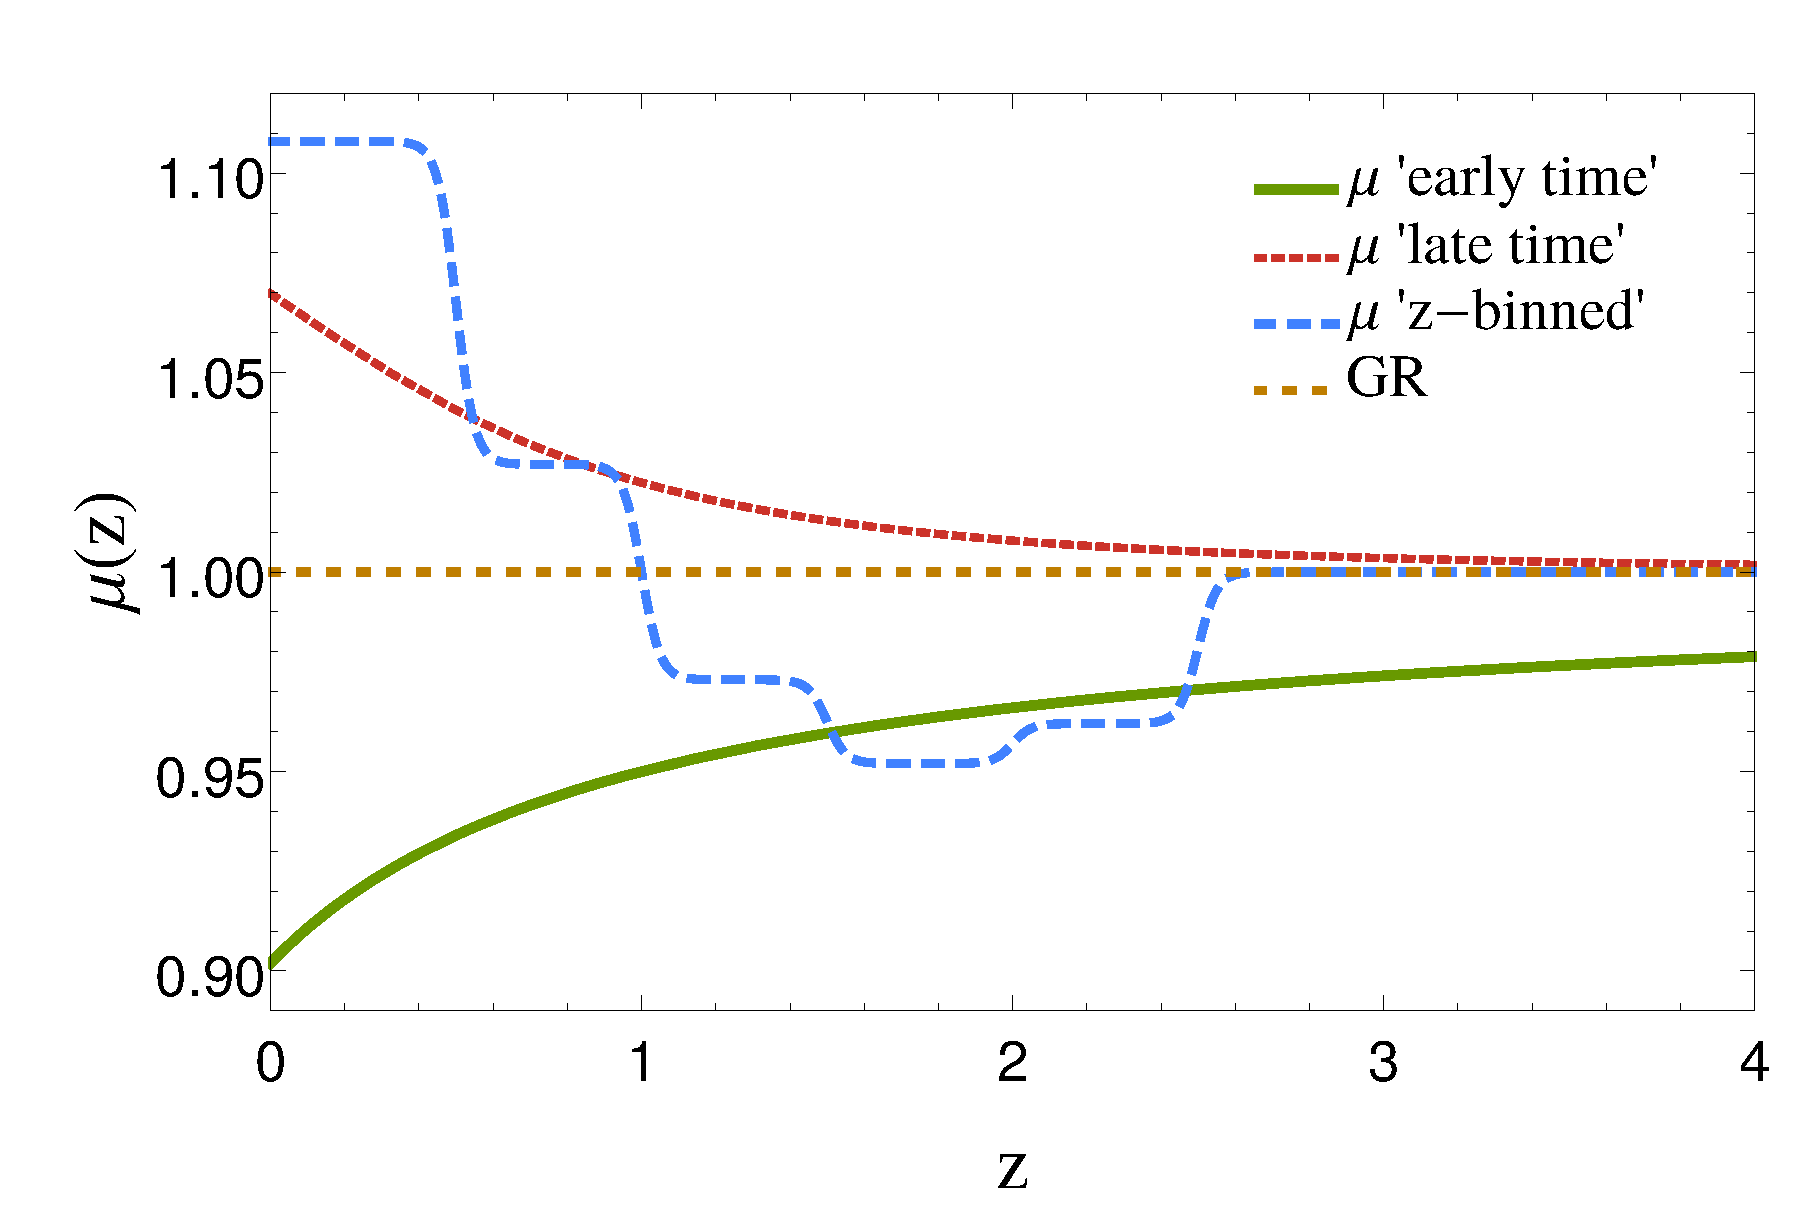
\includegraphics[width=0.45\linewidth]{Chapters/linear-nonlinear-MG-forecasts/figures/fiducials/muFiducialsPlot}
		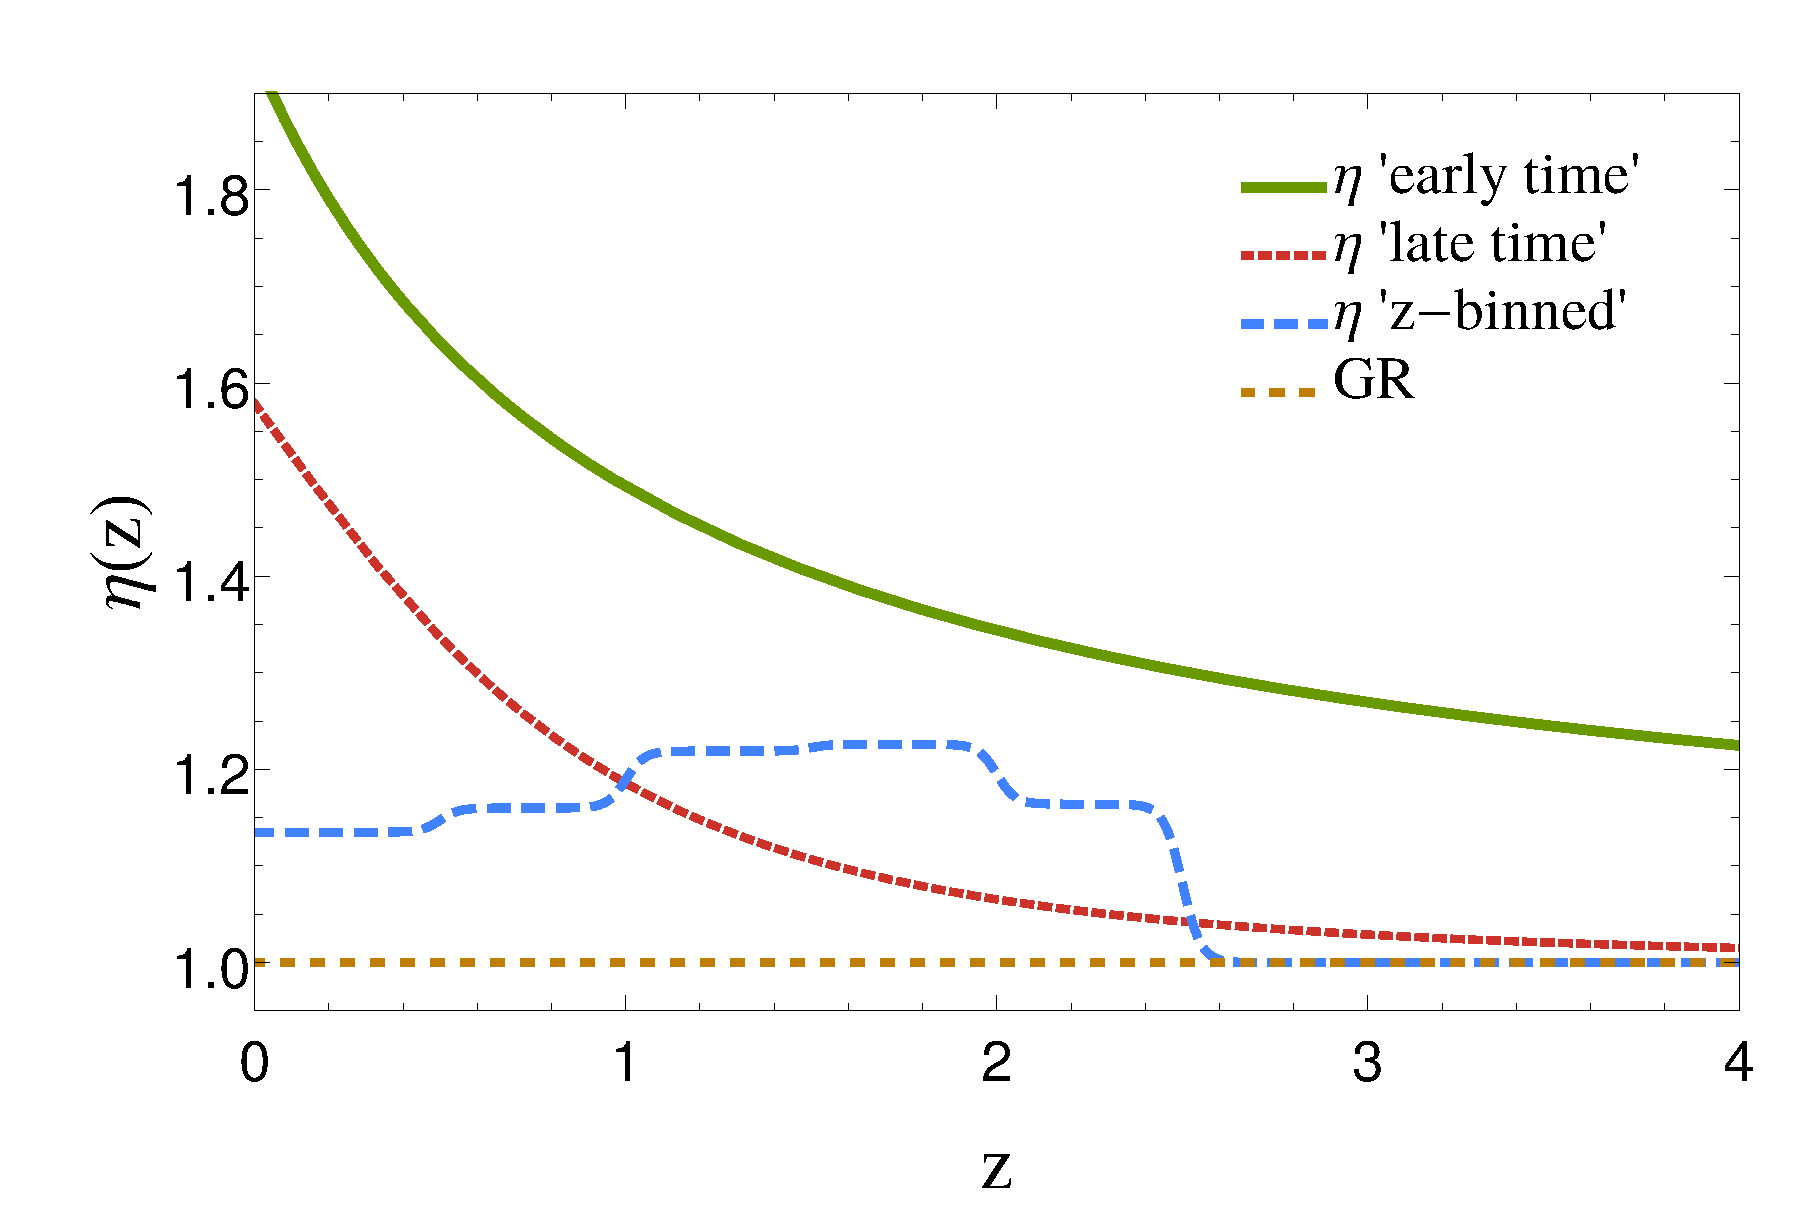
\includegraphics[width=0.45\linewidth]{Chapters/linear-nonlinear-MG-forecasts/figures/fiducials/etaFiducialsPlot}
	\end{center}
	\caption[Modified Gravity functions $\eta$ and $\mu$.]{\label{fig:fidplot}
The Modified Gravity functions $\mu$ and $\eta$ as a function of redshift $z$ for each of the models considered in this work, evaluated at the fiducials specified in \cref{tab:fiducial-MG-AllCases}. 
In light long-dashed blue lines, the `redshift binned model' (\crefrange {eq:MGbin-mu-general-parametrization}{eq:MGbin-muderiv-parametrization}). In short-dashed red lines the late-time parameterization (\crefrange{eq:DE-mu-parametrization}{eq:DE-eta-parametrization}) and in green solid lines the early-time parameterization (\crefrange{eq:TR-mu-parametrization}{eq:TR-eta-parametrization}). Finally the medium-dashed orange line represents the standard $\lcdm$ model (GR) for reference.
		}
\end{figure}


A second and more model-independent approach
is to specify the time evolution of the functions $\mu$ and $\eta$ without
any parameterization. To this purpose we divide the redshift
range $0\leq z\leq3$ in 6 redshift bins and we consider the values
$\mu(z_{i})$ and $\eta(z_{i})$ at the right limiting redshift $z_{i}$
of each bin as free parameters, thus with the $i$ index spanning the values
$\{0.5,1.0,1.5,2.0,2.5,3.0\}$. 
The form of the binning function and the precise assumptions we make, have been specified in \cref{sub:param-z-bins-th}.
%The first bin is assumed to have a constant 
%value, coinciding with the one at $z_1=0.5$, i.e. $\mu(z<0.5)=\mu(z_{1})$ and $\eta(z<0.5)=\eta(z_{1})$.
%The $\mu(z)$ function (and analogously $\eta(z)$) is then reconstructed
%as \todo{this is repeated}
%\begin{equation}\label{eq:MGbin-mu-parametrization}
%\mu(z)=\mu(z_{1})+\sum_{i=1}^{N-1}{\frac{\mu(z_{i+1})-\mu(z_{i})}{2}\left[1+\tanh{\left(s\frac{z-z_{i+1}}{z_{i+1}-z_{i}}\right)}\right]},
%\end{equation}
%where $s=10$ is a smoothing parameter and $N$ is the number of binned
%values. We assume that both $\mu$ and $\eta$ reach the GR limit
%at high redshifts: to realize this, the last $\mu(z_{6})$ and $\eta(z_{6})$
%values assume the standard $\lcdm$ value $\mu=\eta=1$ and both functions
%are kept constant at higher redshifts $z>3$.
We set the first five amplitudes of $\mu_{i}$ and $\eta_{i}$ as
free parameters, thus the set we consider is:
$\theta=\{\Omega_{m},\Omega_{b},h,\ln10^{10} A_{s},n_{s},\{\mu_{i}\},\{\eta_{i}\}\}$,
with $i$ an index going from 1 to 5. We take as fiducial cosmology
the values shown in Tab. \ref{tab:fiducial-MG-AllCases} columns 5
and 6. 

We only modify the evolution of perturbations and assume that
the background expansion is well described by the standard $\Lambda$CDM
expansion law for a flat universe with given values of $\Omega_{m}$,
$\Omega_{b}$ and $h$.




\section{\label{sec:The-non-linear-power}The power spectrum in Modified
Gravity}


\subsection{The linear power spectrum}

In this work we will use linear power spectra calculated with MGCAMB
\cite{zhao_searching_2009,hojjati_testing_2011}, a modified version
of the Boltzmann code CAMB \cite{lewis_efficient_2000}. We do so,
as MGCAMB offers the possibility to input directly any parameterization
of $\mu$ and $\eta$ without requiring further assumptions:
MGCAMB uses \cref{eq:mu_def} and \cref{eq:eta_def} in the Einstein-Boltzmann
system of equations, providing the modified evolution of matter perturbations,
corresponding to our choice of the gravitational potential functions.
Non-relativistic particles like cold dark matter are accelerated by the
gradient of $\Psi$, so that especially the redshift space distortions are
sensitive to the modification given by $\mu(a,k)$. For relativistic particles
like photons and neutrinos on the other hand, the combination of $\Phi+\Psi$ (and therefore $\Sigma$)
enters the equations of motion. The impact on the matter power spectrum
is more complicated, as the dark matter density contrast is linked via
the relativistic Poisson equation to $\Phi$. In addition, an early-time
modification of $\Phi$ and $\Psi$ can also affect the baryon distribution through
their coupling to radiation during that period.
As already mentioned above, we will not consider
the $k-$dependence of $\mu$ and $\eta$ in this work and our modifications
with respect to standard GR will be only functions of the scale factor
$a$.


\subsection{Non-linear power spectra \label{sub:MG-nonlinear-spectra}}

\done\todo{Check that there is not too much repetition}
%As the Universe evolves, matter density fluctuations
%($\delta_{m}$) on small scales (k > 0.1 h/Mpc) become larger than unity and shell-crossing will eventually occur. The usual continuity and
%Euler equations, together with the Poisson equation become singular
%\cite{bernardeau_large-scale_2001,bernardeau_evolution_2013},
%therefore making a computation of the matter power spectrum in the
%highly non-linear regime practically impossible under the standard
%perturbation theory approach. However, at intermediate scales of around
%$k\approx0.1-0.2$ h/Mpc, there is the possibility of calculating
%semi-analytically the effects of non-linearities on the oscillation
%patterns of the baryon acoustic oscillations (BAO). There are many
%approaches in this direction, from renormalized perturbation theories
%\cite{crocce_renormalized_2006,blas_time-sliced_2016,taruya_closure_2008}
%to time flow equations \cite{pietroni_flowing_2008,anselmi_nonlinear_2012}, effective or coarse grained theories
%\cite{carrasco_effective_2012,baumann_cosmological_2012,pietroni_coarse-grained_2011,manzotti_coarse_2014} and many others.
% This direction of research is important, since from the
%amplitude and widths of the first few BAO peaks, one can extract more information from data and break degeneracies among parameters, especially in Modified Gravity.

Computing the non-linear power spectrum in standard GR is still an
open question, and even more so when the Poisson equations are modified,
as it is in the case in Modified Gravity theories. A solution to this problem
is to calculate the evolution of matter perturbations in an N-body
simulation
\cite{springel_cosmological_2005,fosalba_mice_2013,takahashi_revising_2012,lawrence_coyote_2010,heitmann_coyote_2014},
however, this procedure is time-consuming and computationally expensive.

Because of these issues, several previous analyses
have been done with a conservative removal of the information at small
scales (see for example the \planck\ Dark Energy paper
\cite{planck_collaboration_planck_2016},
several CFHTLenS analysis \cite{heymans_cfhtlens_2013,kitching_3d_2014}
or the previous PCA analysis by \cite{hojjati_cosmological_2012}).
However, future surveys will probe an extended range of scales, therefore
removing non-linear scales from the analysis would strongly reduce
the constraining power of these surveys. Moreover, at small scales
we also expect to find means of discriminating between different Modified
Gravity models, such as the onset of screening mechanisms needed to
recover GR at small scales where experiments strongly constrain
deviations from it. For these reasons it is crucial to find methods
which will allow us to investigate, at least approximately, the non-linear
power spectrum.

Attempts to model the non-linear power spectrum semi-analytically in Modified
Gravity have been investigated for f(R) theories in
\cite{zhao_modeling_2014,taruya_regularized_2014},
for coupled dark energy in
\cite{casas_fitting_2015,saracco_non-linear_2010,vollmer_efficient_2014}
and for growing neutrino models in \cite{brouzakis_nonlinear_2011}.
Typically they rely on non-linear expansions of the perturbations
using resummation techniques based on
\cite{pietroni_flowing_2008,taruya_closure_2008}
or on fitting formulae based on N-Body simulations
\cite{casas_fitting_2015,takahashi_revising_2012,bird_massive_2011}.
A similar analysis is not available for the model-independent approach considered
in this chapter. 
In order to give at least a qualitative estimate
of what the importance of non-linearities would be for constraining these
Modified Gravity models, we will adopt in the rest of the chapter a method 
which interpolates between the standard approach to non linear scales in GR
and the same applied to MG theories.

\subsubsection{Halofit}
We describe here the effect of applying the standard 
approach to non linearities to MG theories. This is done using
the revised Halofit \cite{takahashi_revising_2012}, based on
\cite{smith_stable_2003},
which is a fitting function of tens of numerical parameters that reproduces
the output of a certain set of $\lcdm$ N-body simulations in a specific
range in parameter space as a function of the linear power spectrum.
This fitting function is reliable with an accuracy of better than
10\% at scales larger than $k\lesssim1$h/Mpc and redshifts in between
$0\leq z\leq10$ (see \cite{takahashi_revising_2012} for more details).
This fitting function can be used within Boltzmann codes to estimate
the non-linear contribution which corrects the linear power spectrum
as a function of scale and time. We will use the Halofit fitting function
 as a way of approximating the non-linear power spectrum in
our models even though it is really only valid for $\lcdm$. 
In Fig.\ \ref{fig:lin-non-pk-mg}, the left panel
shows a comparison between the linear and non-linear power spectra
calculated by MGCAMB in two different models, our fiducial late-time
model (as from Table \ref{tab:fiducial-MG-AllCases}) and GR, both sharing
the same $\lcdm$ parameters. At small length scales (large $k$),
the non-linear deviation is clearly visible at scales $k\gtrsim0.3$ h/Mpc
and both MG and GR seem to overlap due to the logarithmic scale used.
In the right panel, we can see the ratio between MG and GR for both linear
and non-linear power spectra, using the same 5 $\lcdm$ parameters
$\{\Omega_{m},\Omega_{b},h,\,A_{s},n_{s}\}$. We can see clearly that
MG in the non-linear regime, using the standard Halofit, shows a distinctive
feature at scales in between $0.2\lesssim k\lesssim2$. This feature
however, does not come from higher order perturbations induced by
the modified Poisson equations (\ref{eq:mu_def}, \ref{eq:Sigma-def}),
because Halofit, as explained above, is calibrated with simulations
within the $\lcdm$ model and does not contain any information from
Modified Gravity. The feature seen here is caused by the different
growth rate of perturbations in Modified Gravity, that yields then
a different evolution of non-linear structures. 

\begin{figure}[htbp]
\begin{centering}
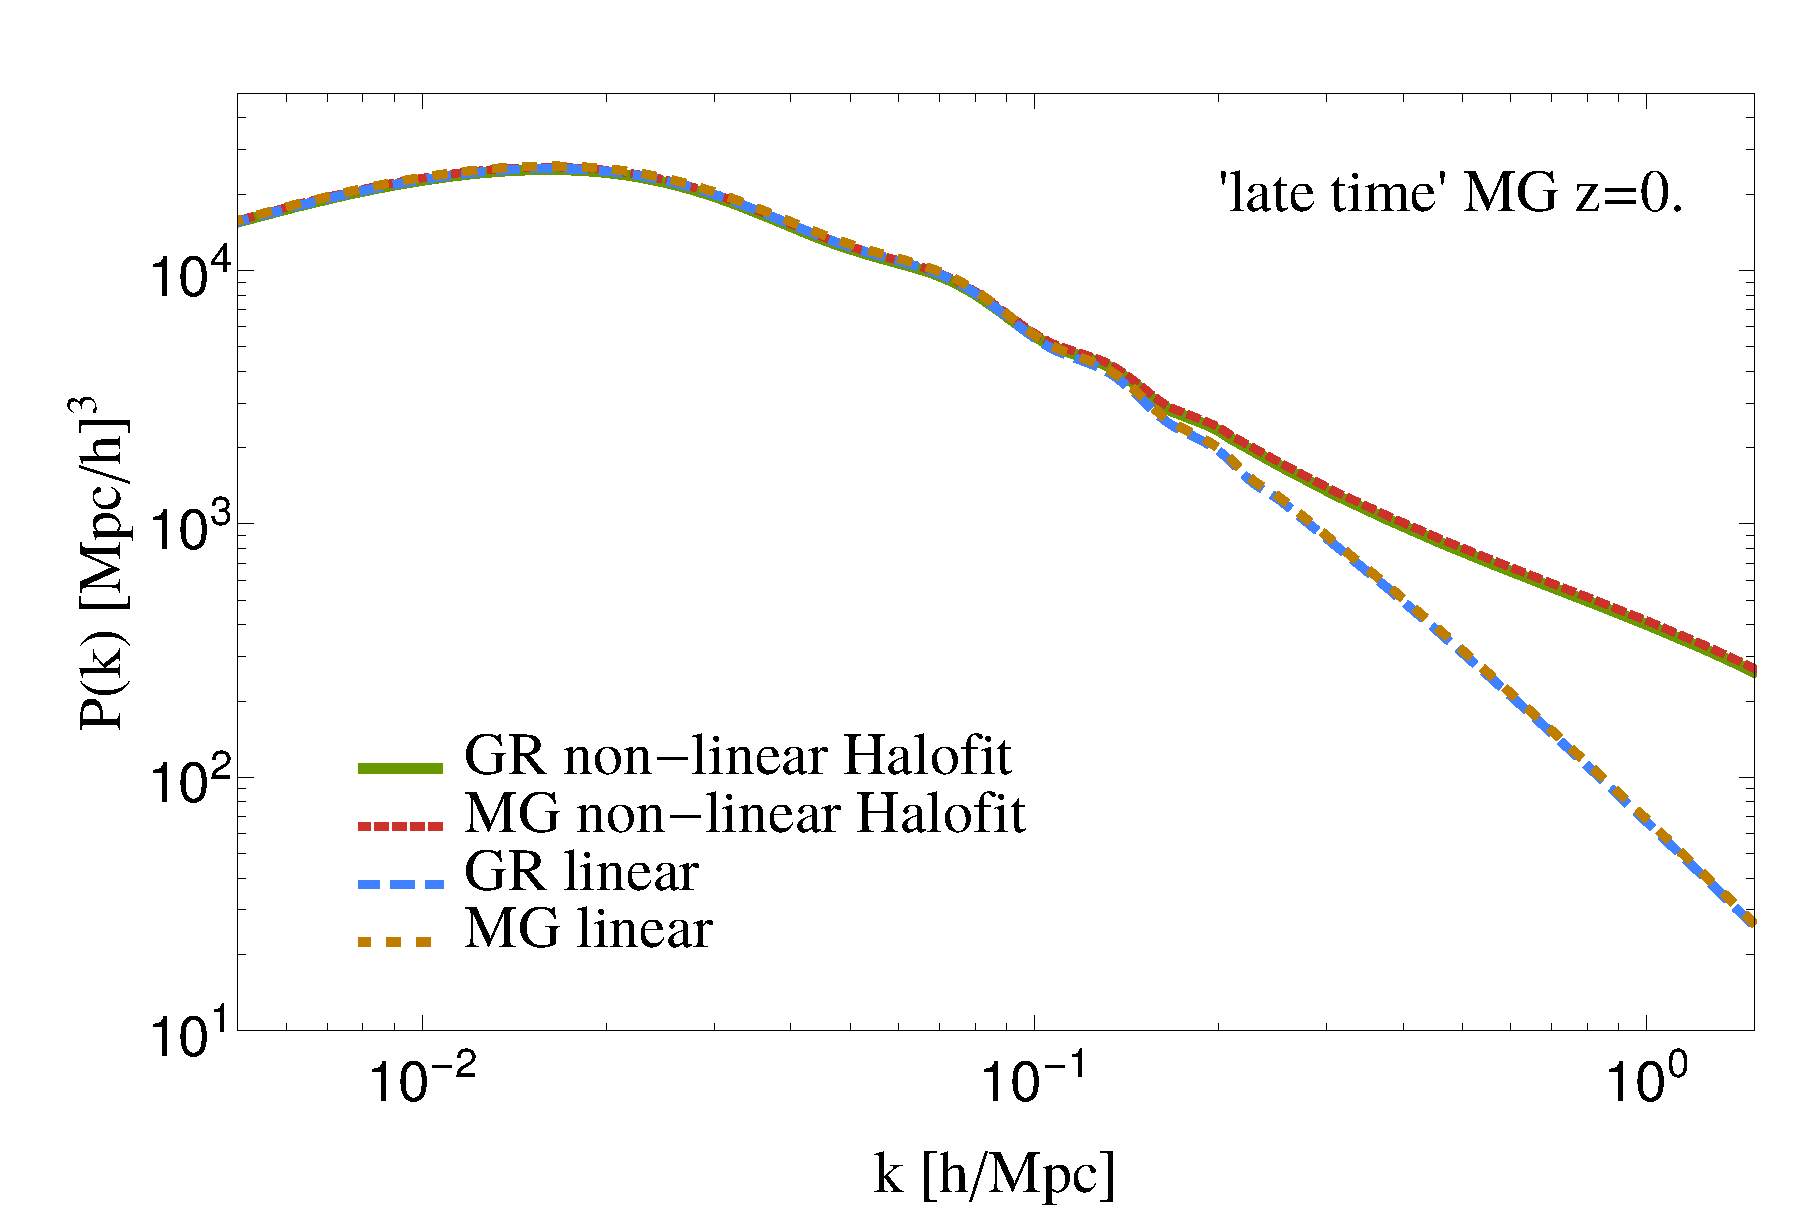
\includegraphics[width=0.45\textwidth]{Chapters/linear-nonlinear-MG-forecasts/figures/power-spectra/pk-GRvsMGDE2nonuhs_Lin-vs-Nonlin-zind_1}
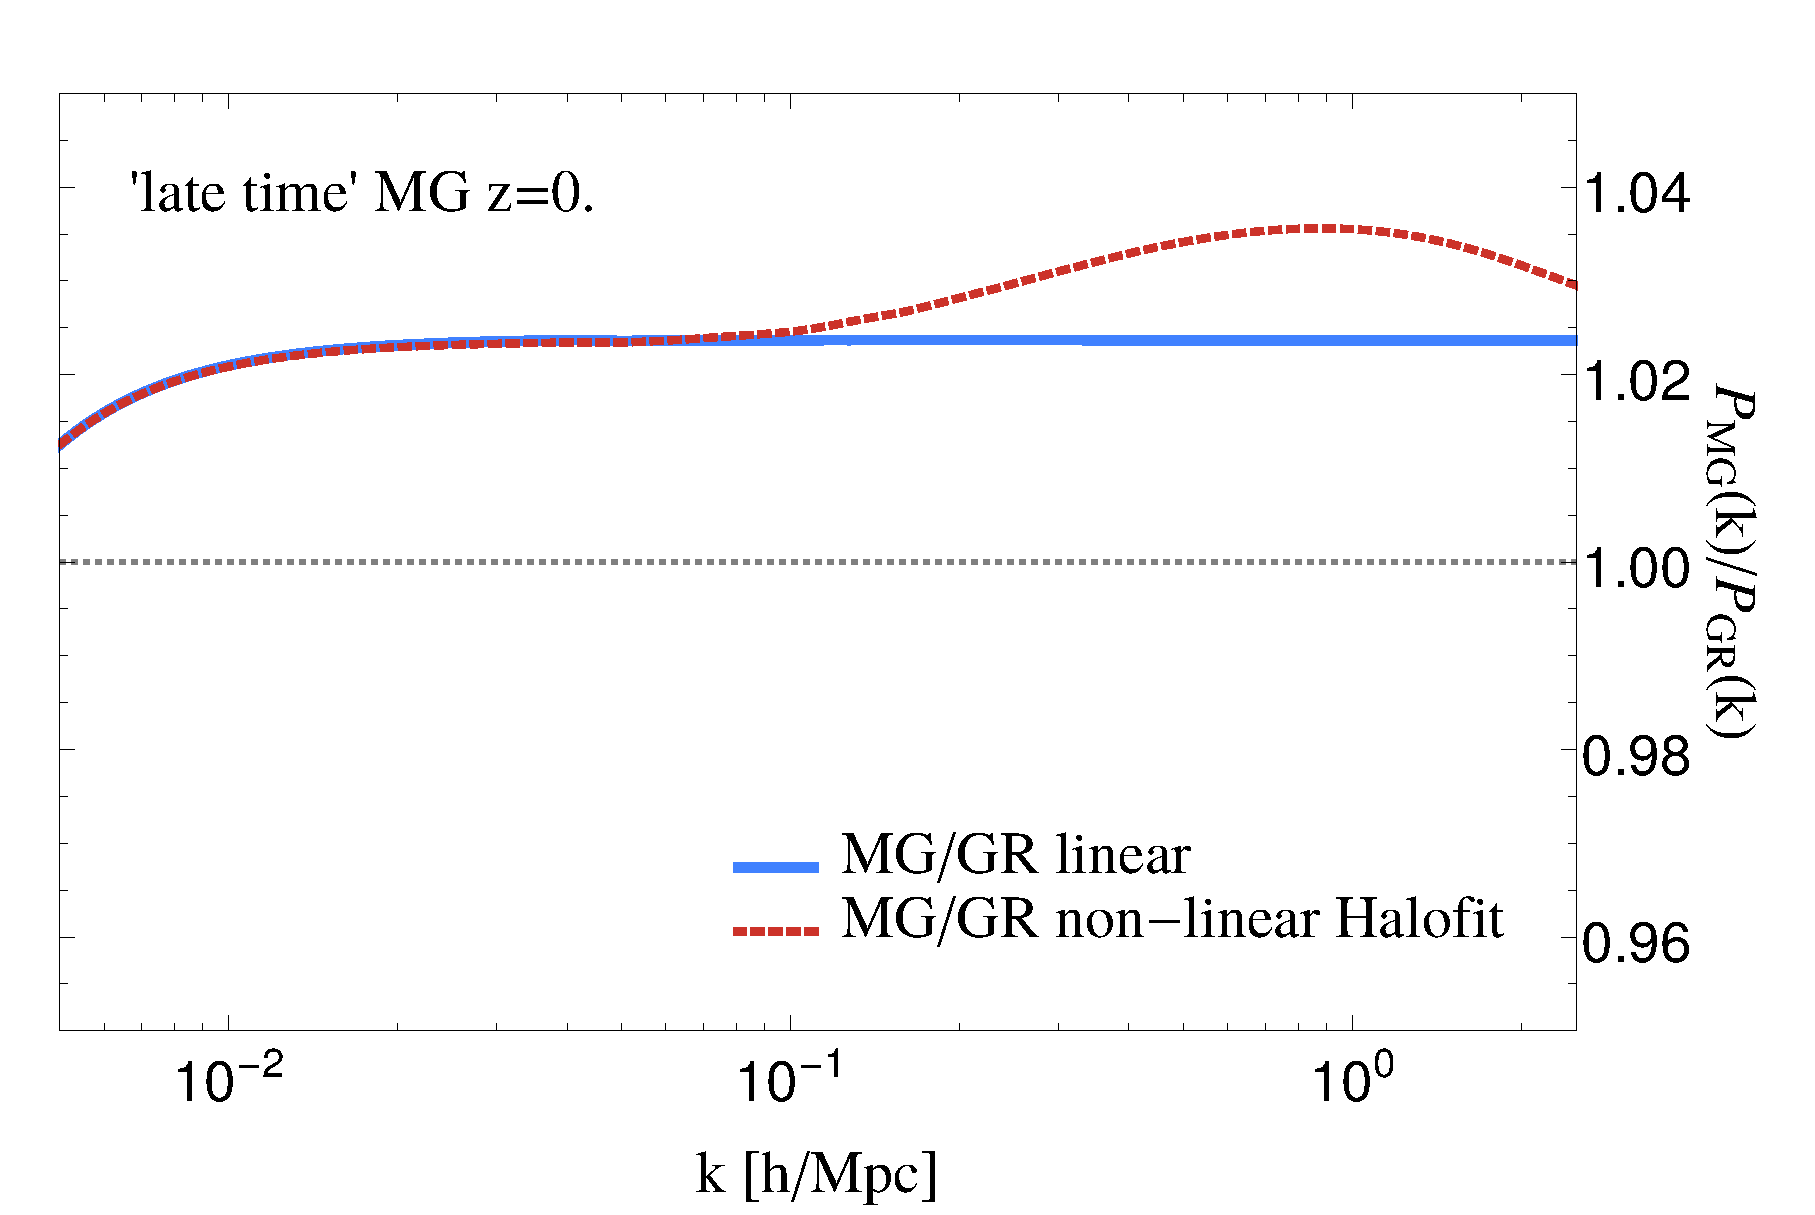
\includegraphics[width=0.45\textwidth]{Chapters/linear-nonlinear-MG-forecasts/figures/power-spectra/pk-Ratios-GRvsMGDE2nonuhs_Lin-vs-Nonlin-zind_1} 
\par\end{centering}
\caption[MGCAMB power spectra, late-time parametrization.]{\label{fig:lin-non-pk-mg} \textbf{Left: }matter power
spectra
computed with MGCAMB (linear) and MGCAMB+Halofit (non-linear), illustrating the impact of non-linearities at different scales. As an illustrative example, MG in this plot corresponds to the fiducial model in the late-time parametrization defined in Eq.\ (\ref{eq:DE-mu-parametrization}).
All curves are computed at $z=0$. The green solid line is the GR
fiducial in the non-linear case, the blue long-dashed line is also
GR but in the linear case. The short-dashed red line is the MG fiducial
in the non-linear case and the medium-dashed brown line the MG fiducial
in the linear case.
\textbf{Right:
}in order to have a closer look at small scales, we plot here the
ratio of the MG power spectrum to the GR power spectrum for the linear
(blue solid) and non-linear (red short-dashed) cases separately. The blue solid line compared to the horizontal grey dashed line,
shows the effect of Modified Gravity when taking only linear spectra into account. While the red dashed line, which
represents the non-linear case, shows that the ratio to GR presents clearly a bump that peaks around
$k\approx1.0$ h/Mpc, meaning that the power spectrum in MG differs
at most 4\% from the non-linear power spectrum in GR. We will see later that we are able to 
discriminate between these two models using future surveys, especially when non-linear scales ($k \gtrsim 0.1$ h/Mpc) are included.
} 
\end{figure}



\subsubsection{Prescription for mildly non-linear scales including screening}
\label{sub:Prescription-HS}

As discussed above, modifications to the $\Phi$ and $\Psi$ 
potentials make the use of Halofit to compute the evolution at non linear scales 
unreliable. In order to
take into account the non-linear contribution to the power spectrum
in Modified Gravity, we investigate here a different method, which
starts from the consideration that whenever we
modify $\mu$ and $\eta$ with respect to GR, we modify the strength
of gravitational attraction in a way universal to all species: this
means that, similarly to the case of scalar-tensor or $f(R)$ theories,
we need to assume the existence of a non-perturbative screening mechanism, acting at
small scales, that guarantees agreement with solar system experiments.
In other words, it is reasonable to think that the non-linear power
spectrum will have to match GR at sufficiently small scales, while
at large scales it is modified. Of course, without having a specific model in mind, it remains arbitrary
how the interpolation between the small scale regime and the large
scale regime is done. In this
chapter, we adopt the Hu \& Sawicki (HS) Parametrized Post-Friedmann prescription proposed
in \cite{hu_parameterized_2007}, which was used for the case of $f(R)$
theories previously by \cite{zhao_modeling_2014}. Given a MG model,
this prescription interpolates between the non-linear power spectrum
in Modified Gravity (which is in our case just the linear MG power
spectrum corrected with standard Halofit, $P_{\HMG}$) and the non-linear
power spectrum in GR calculated with Halofit ($P_{\mathrm{HGR}}$). The resulting
power spectrum will be denoted as $P_{\mathrm{nlHS}}$
\begin{equation}
P_{\mathrm{nlHS}}(k,z)=\frac{P_{\HMG}(k,z)+\cnl S_{\LIN}^{2}(k,z)P_{\mathrm{HGR}}(k,z)}{1+\cnl S_{\LIN}^{2}(k,z)} \, ,\label{eq:PHSDefinition}
\end{equation}
with 
\begin{equation}
S_{\LIN}^{2}(k,z)=\left[\frac{k^{3}}{2\pi^{2}}P_{\LMG}(k,z)\right]^{s} \, . \label{eq:prescription_sigma_def}
\end{equation}
The weighting function $S_{\LIN}$ used in the interpolation quantifies the onset of non-linear clustering and it is constructed
using the linear power spectrum in Modified Gravity ($P_{\LMG}$).
The constant $\cnl$ and the constant exponent $s$ are free parameters.
In Figure \ref{fig:lin-nonlin-Zhao-MG} we show the ratio $P_{\mathrm{nlHS}}/P_{\HGR}$,
which illustrates the relative difference between the non-linear HS prescription
in MG and the Halofit non-linear power spectrum in GR, for different
values of $\cnl$ (left panel) and different values of $s$ (right
panel). The parameter $\cnl$ controls at which scale there is a
transition into a non-linear regime in which standard GR is valid
(this can be the case when a screening mechanism is activated);
$s$ controls the smoothness of the transition and is in principle
a model and redshift dependent quantity. When $\cnl=0$ we recover
the Modified Gravity power spectrum with Halofit $P_{\HMG}$; when
$\cnl\rightarrow\infty$ we recover the non-linear power spectrum
in GR calculated with Halofit $P_{\mathrm{HGR}}$. In
\cite{zhao_modeling_2014,zhao_n-body_2011,koyama_non-linear_2009},
the $\cnl$ and $s$ constants were obtained fitting expression (\ref{eq:PHSDefinition}) to N-Body
simulations or to a semi-analytic perturbative approach. In the case
of $f(R)$, $s=1/3$ seems to match very well the result from simulations
up to a scale of $k=0.5$h/Mpc \cite{koyama_non-linear_2009}. A relatively
good agreement up to such small scales is enough for our purposes.
In the absence of N-Body simulations or semi-analytic methods available
for the models investigated in this work, we will assume unity for
both parameters, which is a natural choice, and we will test in Section \ref{sub:Testing-the-effect-of-Zhao}
how our results vary for different values of these parameters, namely
$\cnl=\{0.1,0.5,\,1,3\}$ and $s=\{0,\,1/3,\,2/3,\,1\}$. This will
give a qualitative estimate of the impact of non-linearities on the
determination of cosmological parameters.

\begin{figure}[htbp]
\begin{centering}
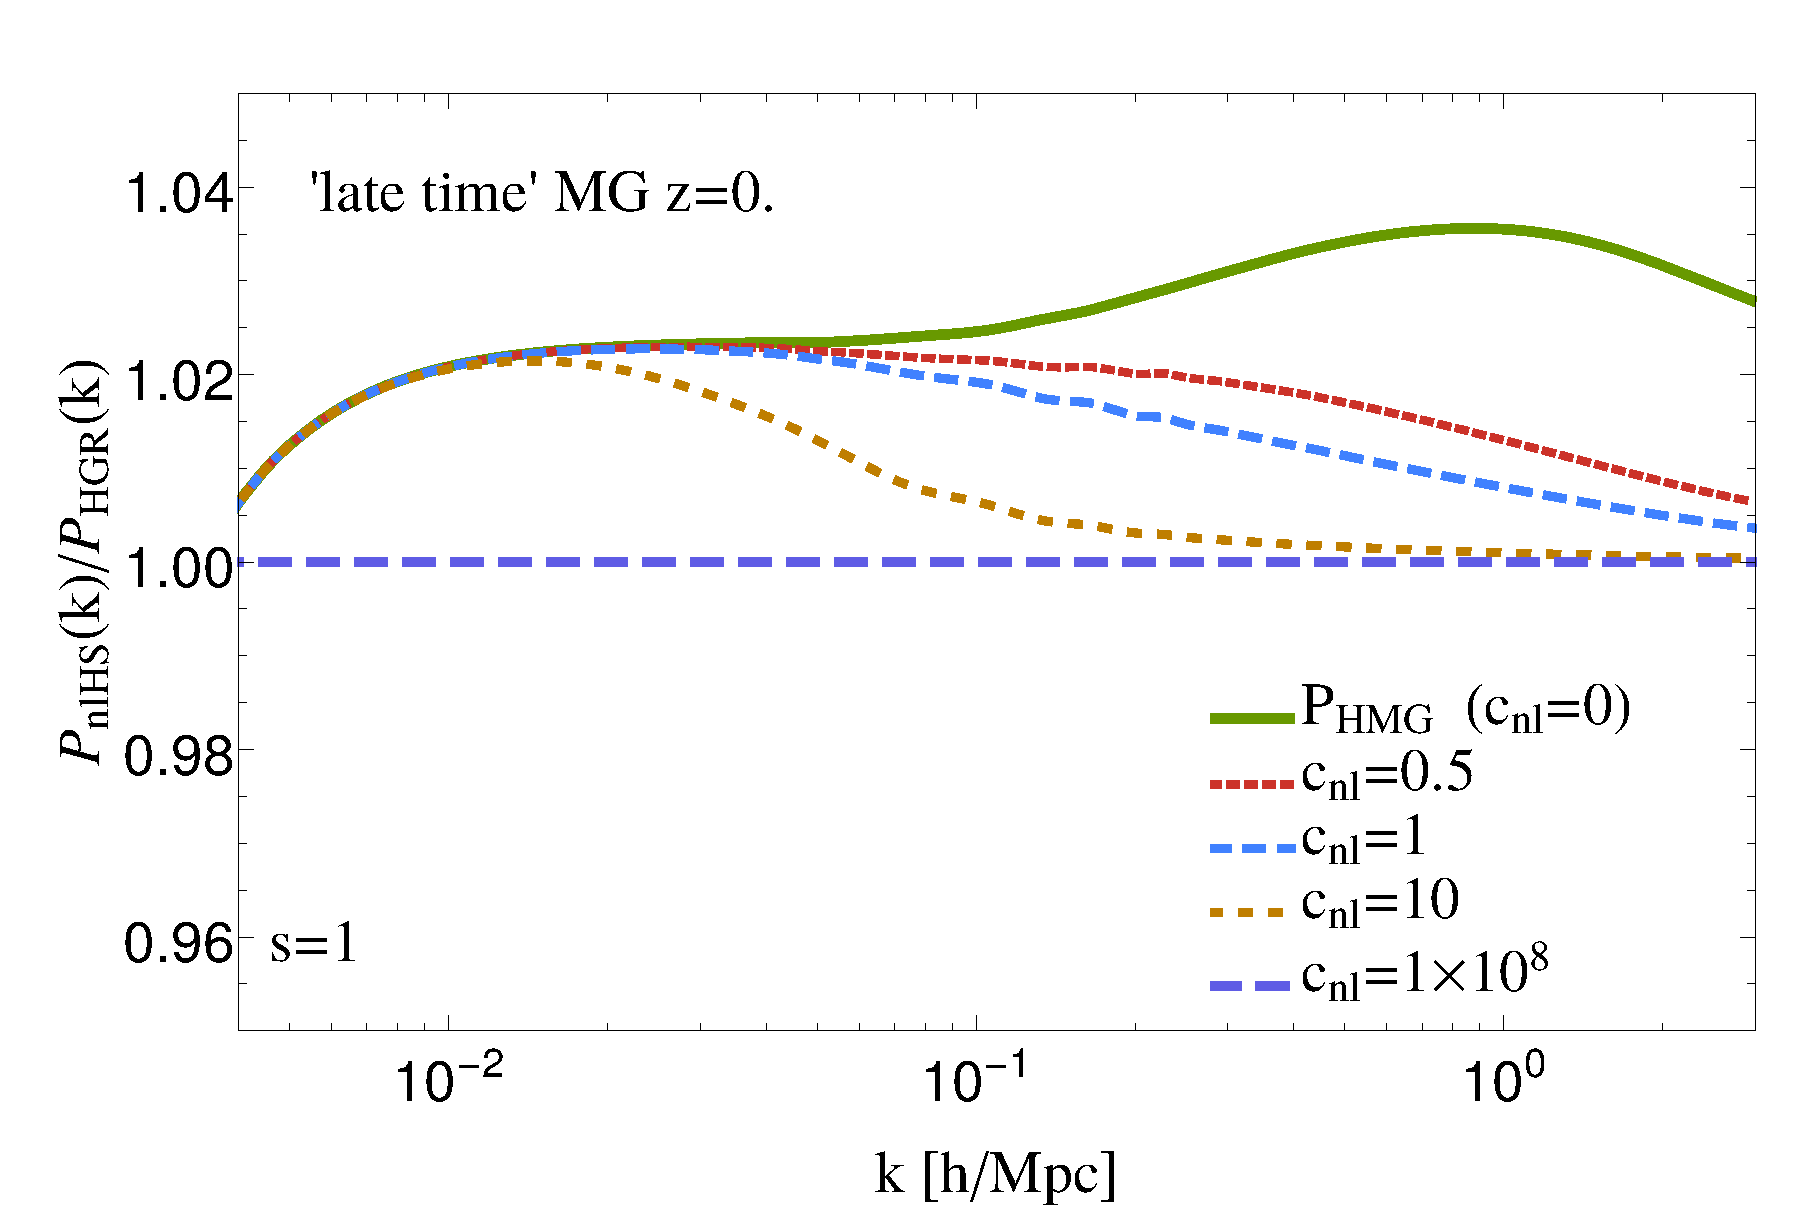
\includegraphics[width=0.45\textwidth]{Chapters/linear-nonlinear-MG-forecasts/figures/power-spectra/pk-Ratios-ZhaovsGRNL-MGDE2nonuhs-z_0p-zind_1}
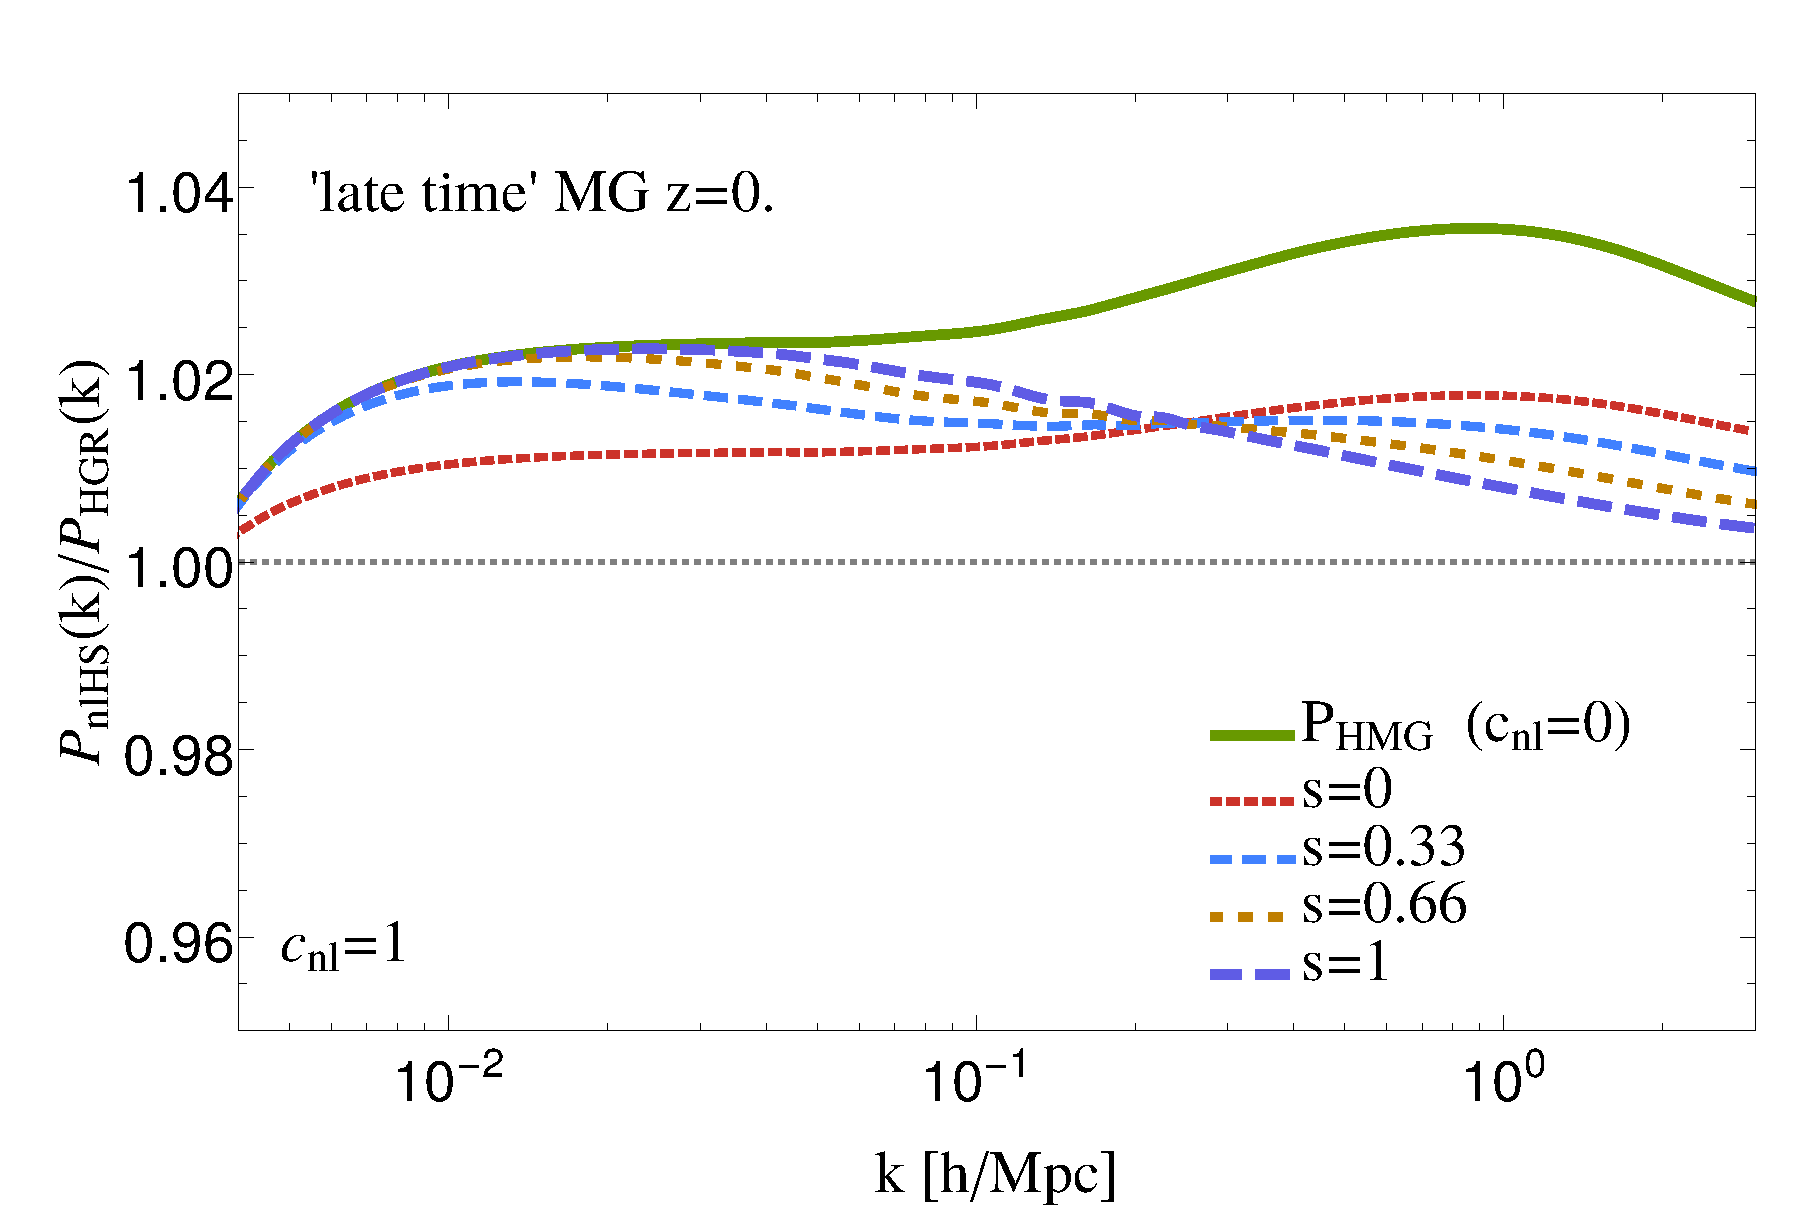
\includegraphics[width=0.45\textwidth]{Chapters/linear-nonlinear-MG-forecasts/figures/power-spectra/pk-Ratios-Zhao_SigmaExp-vsGRNL-MGDE2nonuhs-z_0p-zind_1} 
\end{centering}
\caption[Effect of the non-linear Hu\&\ Sawicki prescription]{\label{fig:lin-nonlin-Zhao-MG} The ratio of the Modified Gravity non-linear
power spectrum using the HS prescription by \cite{hu_parameterized_2007}
($P_{\mathrm{nlHS}}$) with respect to the GR+Halofit fiducial non-linear power spectrum $P_{\mathrm{HGR}}$, 
for different values of $\cnl$ (left panel) and $s$ (right panel),
illustrated in \cref{eq:PHSDefinition} and \cref{eq:prescription_sigma_def}.
The value $\cnl=0$ (green solid line) corresponds
to MG+Halofit $P_{\HMG}$.
All curves are calculated at $z=0$.
\textbf{Left: } We show the ratio for $\cnl=\{0.5,1.0,10,10^8\}$,
plotted as short-dashed red, medium-dashed blue, short-dashed brown and medium-dashed purple
lines respectively. When $\cnl\rightarrow\infty$, \cref{eq:PHSDefinition}
corresponds to the limit of $P_{\HGR}$ and therefore the ratio is
just 1. The effect of the HS prescription
is to grasp some of the features of the non-linear power spectrum
at mildly non-linear scales induced by Modified Gravity, taking into
account that at very small scales, a screening mechanism might yield
again just a purely GR non-linear power spectrum. The parameter $\cnl$
interpolates between these two cases. \textbf{Right: }in this panel
we show the effect of the parameter $s$, for $s=\{0,0.33,0.66,1\}$
(short-dashed red, medium-dashed blue, short-dashed brown and long-dashed
purple, respectively). Both parameters need to be fitted with simulations
in order to yield a reliable match with the shape of the non-linear
power spectrum in Modified Gravity, as it was done in \cite{zhao_n-body_2011}
and references therein. The grey dashed line marks the constant value of 1.}
\end{figure}


\subsection{CMB \planck\ priors}
\label{sub:Fisher-Planck}
Alongside the information brought by LSS probes,
we also include CMB priors on the parameterizations considered. In
order to obtain these, we analyze the binned and parameterized approaches
described in \cref{sub:parameterizing-MG} with
the {\it Planck}+BSH combination of CMB and background (BAO+SN-Ia+$H_{0}$)
datasets discussed in the \planck\ Dark Energy and Modified Gravity paper
\cite{planck_collaboration_planck_2016}.
We use a Markov Chain Monte Carlo (MCMC) approach, using the publicly
available code \texttt{COSMOMC} \cite{lewis_cosmological_2002,lewis_efficient_2013},
interfaced with our modified version of \texttt{MGCAMB}. The MCMC
chains sample the parameter vector $\Theta$ which contains the standard
cosmological parameters
$\{\omega_{b}\equiv\Omega_{b}h^{2},\,\omega_{c}\equiv\Omega_{c}h^{2},\,\theta_{\rm MC},\,\tau,n_{s},\ln{10^{10}A_{s}}\}$
to which we add the $E_{ij}$ parameters when we parameterize the time
evolution of $\mu$ and $\eta$ with continuous functions of the scale factor, 
and the $\mu_{i},\ \eta_{i}$ parameters in the binned
case. On top of these, also the 17 nuisance parameters of the \planck\
analysis are included. From the MCMC analysis of the \planck\ likelihood
we obtain a covariance matrix in terms of the parameters $\Theta$.
We marginalize over the nuisance parameters and over the optical
depth $\tau$ since this parameter does not enter into
the physics of large scale structure formation.

$\theta$ is usually the ratio of sound horizon
to the angular diameter distance at the time of decoupling. Since
calculating the decoupling time $z_{\rm CMB}$ is relatively time consuming,
as it involves the minimization of the optical transfer function,
\texttt{COSMOMC} uses instead an approximate quantity $\theta_{\rm MC}$
based on the following fitting formula from \cite{hu_small_1996}
\begin{align}
z_{\rm CMB} & =1048\times(1+0.00124\omega_{b}^{-0.738})\nonumber \\
&
\times\left(1+0.0783\omega_{b}^{-0.238}/(1+39.5\omega_{b}^{0.763})\right.\nonumber
\\
& \times\left.(\omega_{d}+\omega_{b})^{0.560/(1+21.1\omega_{b}^{1.81})}\right)
\end{align}
where $\omega_{d}\equiv(\Omega_{c}+\Omega_{\nu})h^{2}$.
The sound horizon is defined as 
\begin{equation}
r_{s}(z_{\rm CMB})=cH_{0}^{-1}\int_{z_{\rm CMB}}^{\infty}\mbox{d}z\frac{c_{s}}{E(z)}
\end{equation}
where the sound speed is $c_{s}=1/\sqrt{3(1+\overline{R}_{b}a)}$with
the baryon-radiation ratio being $\overline{R}_{b}a=3\rho_{b}/4\rho_{\gamma}$.
$\overline{R}_{b}=31500\Omega_{b}h^{2}(T_{\rm CMB}/2.7\mbox{K})^{-4}$.
However, \texttt{CAMB }approximates it as
$\overline{R}_{b}a=30000a\Omega_{b}h^{2}$.

Therefore we first marginalize the covariance matrix over the nuisance
parameters and the parameter $\tau$, which cannot be constrained
by LSS observations. Then, we invert the resulting matrix, to obtain a \planck\
prior Fisher matrix and then use a Jacobian to convert between the
MCMC parameter basis $\Theta_{i}$ and the GC-WL parameter basis $\theta_{i}$.
We use the formulas above for the sound horizon $r_{s}$ and the angular
diameter distance $d_{A}$ to calculate the derivatives of $\theta_{\rm MC}$
with respect to the parameters of interest. Our Jacobian is then simply
\begin{equation}
J_{ij}=\frac{\partial\Theta_{i}}{\partial\theta_{j}} \, .
\end{equation}


\subsection{Jacobian for the late time parameterization \label{subsub:Jacobian}}
Our main observables are parameterized
in terms of the primary variables $E_{11}$ and $E_{22}$ from Equation
\ref{eq:TR-mu-parametrization}; we are however interested in forecasting
the constraints on the pair of secondary variables $\{\mu$, $\eta\}$
or on the pair $\{\mu$, $\Sigma$\}.

Therefore we need to transform the variables using a Jacobian
$J_{ij}=\partial\theta_{i}/\partial\tilde{\theta}_{j}$,
where $\theta_{i}$ is the set of primary variables and $\tilde{\theta}_{i}$
is the vector of secondary variables. 
Eqns. (\ref{eq:SigmaofMuEta},\ref{eq:DE-mu-parametrization},\ref{eq:DE-eta-parametrization})
allow us to express the $\tilde{\theta}_{i}$ as a function of the variables $\theta_{i}$ and 
to obtain the non-vanishing derivatives
of $\mu$ and $\eta$ w.r.t to all cosmological parameters:

\begin{alignat}{2}
\frac{\partial\mu}{\partial\Omega_{c}} & =-E_{11},\qquad &
\frac{\partial\eta}{\partial\Omega_{c}} & =-E_{22}\\
\frac{\partial\mu}{\partial\Omega_{b}} & =-E_{11},\qquad &
\frac{\partial\eta}{\partial\Omega_{b}} & =-E_{22}\\
\frac{\partial\mu}{\partial E_{11}} &
=1-\Omega_{b}-\Omega_{c}-\Omega_{\nu},\qquad & \frac{\partial\eta}{\partial
	E_{22}} & =1-\Omega_{b}-\Omega_{c}-\Omega_{\nu} \,\,\, .
\end{alignat}
With these derivatives we can construct the inverse of the Jacobian
$J_{ij}^{-1}=\partial\tilde{\theta}_{j}/\partial\theta_{i}$.
The Fisher matrix in the secondary variables $\tilde{F}{}_{ij}$ is
then given by 
\begin{equation}
\tilde{F}=J^{T}F\,J
\end{equation}
For the parameter set containing $\tilde{\theta}_{i}=\{\mu,\Sigma\}$
we obtain the following non-vanishing derivatives 
\begin{alignat}{2}
\frac{\partial\mu}{\partial\Omega_{c}}  = & -E_{11}, \quad \frac{\partial\mu}{\partial\Omega_{b}}  =-E_{11} ,\quad \frac{\partial\mu}{\partial E_{11}} 
=1-\Omega_{b}-\Omega_{c}-\Omega_{\nu} & &\\
\frac{\partial\Sigma}{\partial\Omega_{c}} 
= & -\frac{1}{2}E_{22}(1+E_{11}(1-\Omega_{b}-\Omega_{c}-\Omega_{\nu})) & &\\
& -\frac{1}{2}E_{11}(2+E_{22}(1-\Omega_{b}-\Omega_{c}-\Omega_{\nu})) &  & \nonumber \\
\frac{\partial\Sigma}{\partial\Omega_{b}}
= &  \frac{\partial\Sigma}{\partial\Omega_{c}}  \\
\frac{\partial\Sigma}{\partial E_{11}} 
= & \frac{1}{2}(2+E_{22}(1-\Omega_{b}-\Omega_{c}-\Omega_{\nu}))
(1-\Omega_{b}-\Omega_{c}-\Omega_{\nu}) & & \\
\frac{\partial\Sigma}{\partial E_{22}} 
= & \frac{1}{2}(1+E_{11}(1-\Omega_{b}-\Omega_{c}-\Omega_{\nu}))
(1-\Omega_{b}-\Omega_{c}-\Omega_{\nu}) & &
\end{alignat}

\subsection{Jacobian for the early time parameterization}

In the early time case, we have two parameters for each $\mu(a)$
and $\eta(a)$ function as in Eq.\ (\ref{eq:TR-mu-parametrization}).
If we are interested in the parameters $\mu$, $\eta$ and $\Sigma$
today ($a=1$), then the parameters $E_{12}$ and $E_{21}$ are not
important anymore and we can simply marginalize over them in our Fisher
matrix. Then the relation between $\mu$ and $\eta$ is very simple
$\{\mu,\eta\}=1+\{E_{11},\,E_{22}\}$. The corresponding Jacobian
is simply a $7\times7$ identity matrix and we can apply it to the
Fisher matrix after we marginalize over the two unimportant parameters.

For the transformation to the pair $\mu$-$\Sigma$ we use the definition
of $\Sigma$ of Eq.\ (\ref{eq:SigmaofMuEta}) and then find the derivatives
with respect to $E_{ij}$. We obtain

\begin{align}
\frac{\partial\Sigma}{\partial E_{11}} & =\frac{1}{2}(2+E_{22})\\
\frac{\partial\Sigma}{\partial E_{22}} & =\frac{1}{2}(2+E_{11})\quad,
\end{align}
while all other derivatives remain the same.


\section{\label{sec:Results:-Redshift-Binned}Results: Euclid forecasts for redshift binned parameters}
In this section we analyze the Modified Gravity functions $\mu(a)$ and $\eta(a)$,
described in Section \ref{sub:parameterizing-MG}, when they are allowed
to vary freely in five redshift bins.

For this purpose, we calculate a Fisher matrix of fifteen parameters:
five for the standard $\lcdm$ parameters $\{\Omega_{m},\Omega_{b},h,\ln10^{10}A_{s},n_{s}\}$,
five for $\mu$ (one
for each bin amplitude $\mu_{i}$) and five for $\eta$ (one for each
bin amplitude $\eta_{i}$), corresponding to the 5 redshift bins z=\{0-0.5, 0.5-1.0, 1.0-1.5, 1.5-2.0, 2.0-2.5\}. 
The fiducial values for all fifteen parameters
were calculated running a Markov-Chain-Monte-Carlo with \planck\ likelihood
data and can be found in Table \ref{tab:fiducial-MG-AllCases}.

We first show the constraints on our 15 parameters for Galaxy Clustering (GC) forecasts in subsection \ref{sub:GC-Correlations},
while in subsection \ref{sub:Weak-Lensing} we report results for Weak Lensing (WL). In subsection \ref{sub:Combined-GC-WL-Planck-Binned}, we
comment on the combination of forecasts for GC+WL together with \planck\ data.
All forecasts are performed using Euclid Redbook specifications. 
Other surveys 
will be considered for the other two time parameterizations in section \ref{subsub: other-surveys-late-time} and 
\ref{subsub: other-surveys-early-time}. 
For each case, we show the correlation matrix obtained from the covariance matrix and argue that 
the redshift-binned
parameters show a strong correlation, therefore we illustrate the decorrelation
procedure for the covariance matrix in  \cref{sec:Decorrelation-of-covariance}
where we also include combined GC+WL and GC+WL+{\it Planck} cases.



\subsection{\label{sub:GC-Correlations}Euclid Galaxy Clustering Survey}


For the Galaxy Clustering survey, we give results for two cases, one
using only linear power spectra up to a maximum wavevector of $k_{\rm max}=0.15$
h/Mpc and another one using non-linear power spectra up to $k_{\rm max}=0.5$
h/Mpc, as obtained by using the HS parameterization of
Eqn.\ (\ref{eq:PHSDefinition}).
For the redshift-binned case, we will report forecasts only for a Euclid survey, 
using Euclid Redbook specifications which
are detailed in section \ref{sub:Fisher-Galaxy-Clustering}.

\begin{figure}[htbp]
\centering
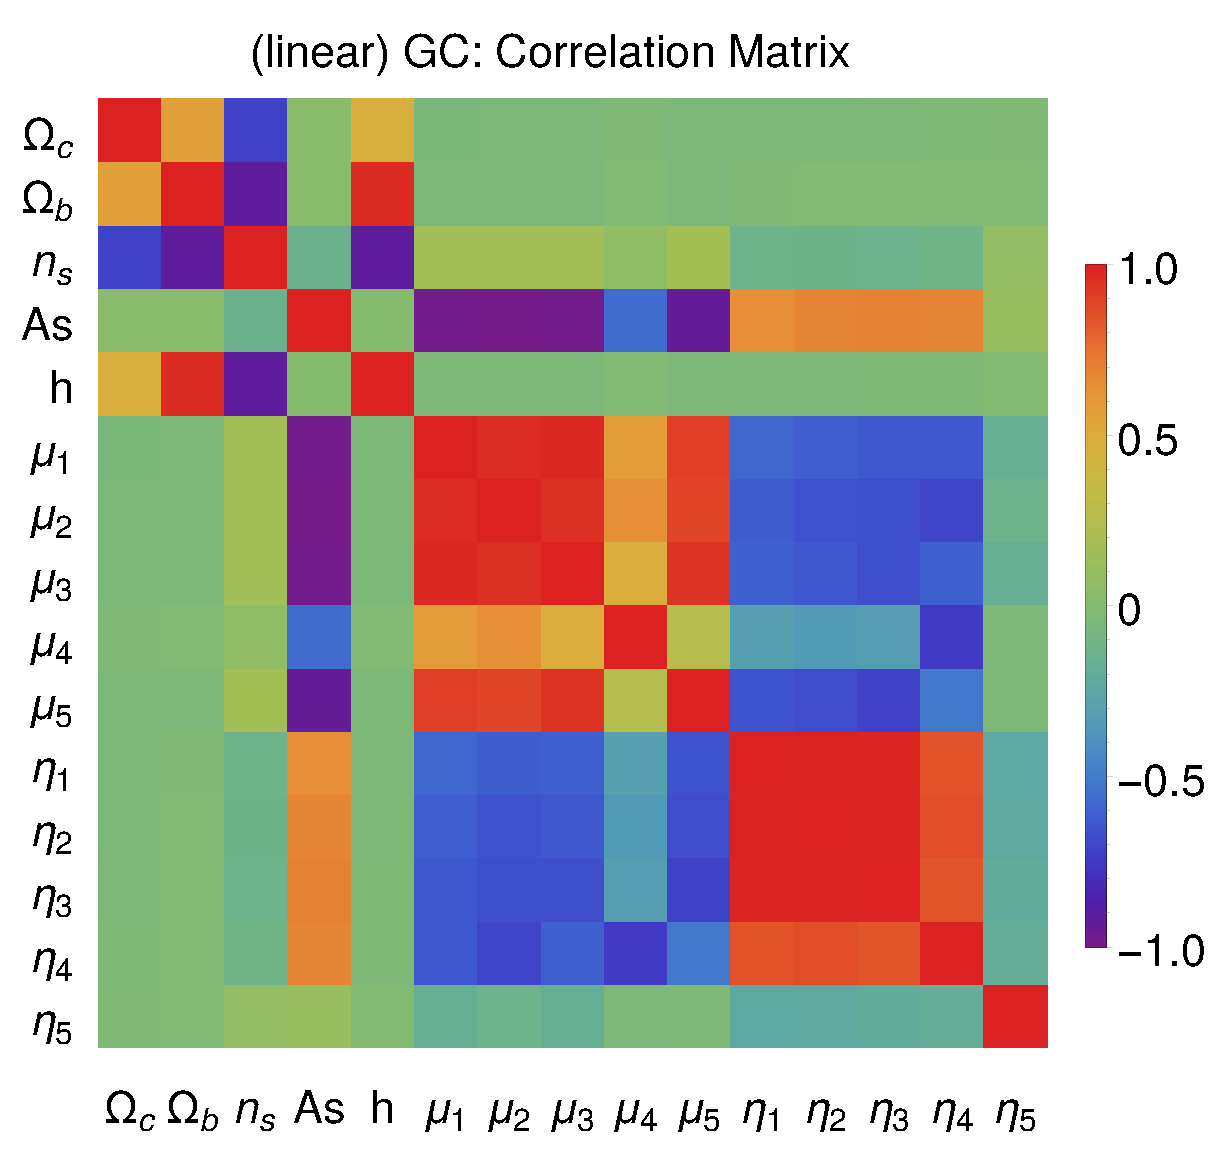
\includegraphics[width=0.47\textwidth]{Chapters/linear-nonlinear-MG-forecasts/figures/Decorrelations-GC/correlation-full-fiducialMGBin3-Euclid-GC-linearPK-}
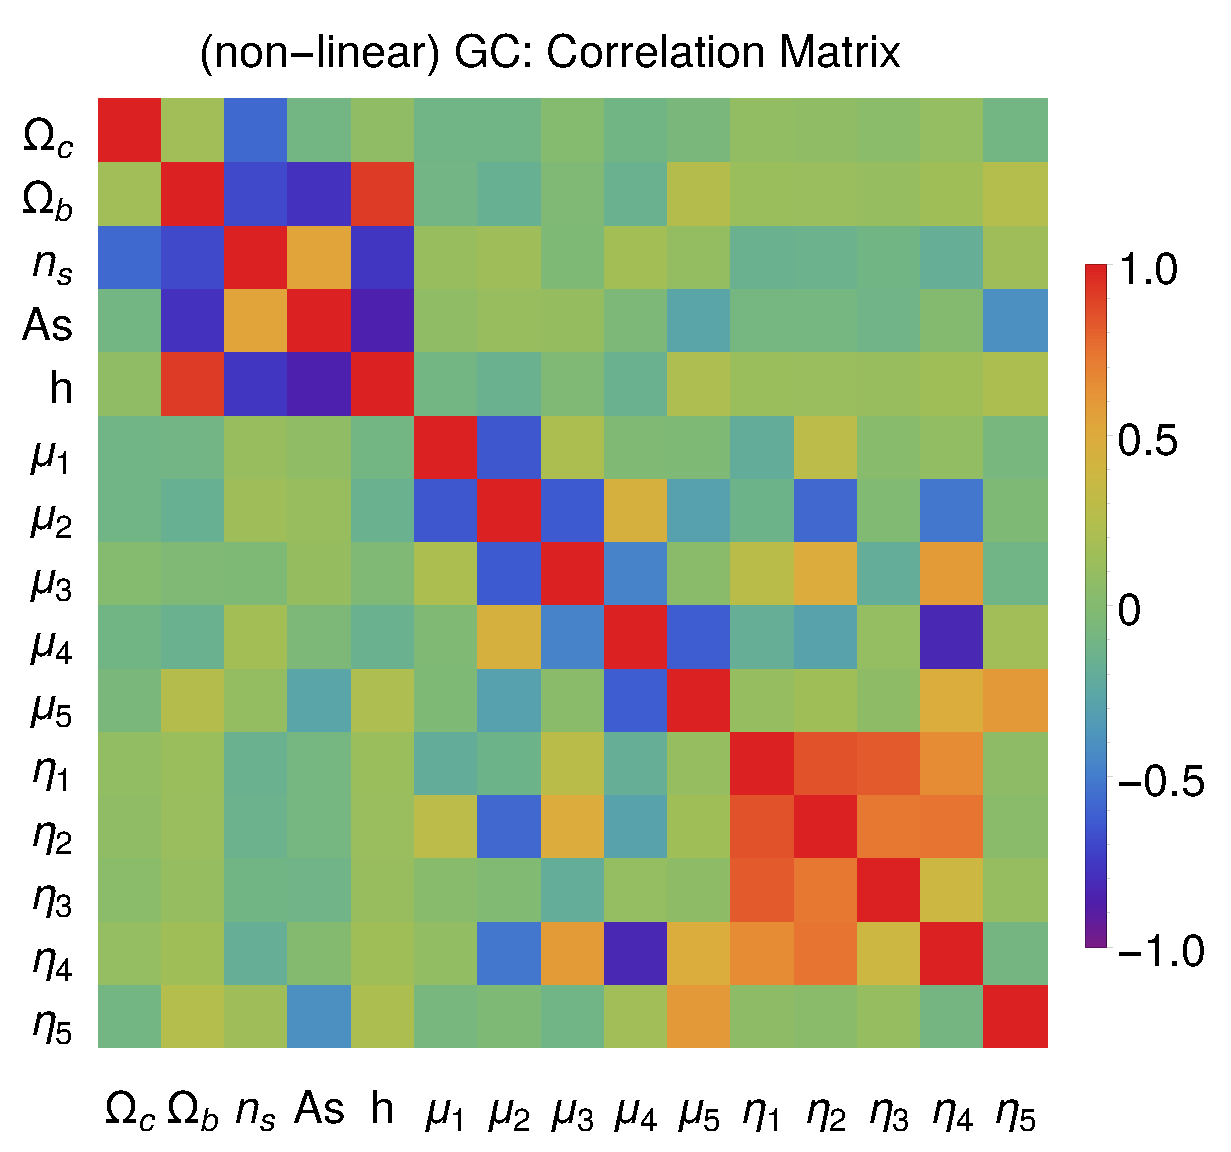
\includegraphics[width=0.47\textwidth]{Chapters/linear-nonlinear-MG-forecasts/figures/Decorrelations-GC/correlation-full-fiducialMGBin3-Euclid-GC-nonlinearPk__Zhao-}
\caption[Correlation matrices for a Euclid Galaxy Clustering forecast.]{\label{fig:GCcorr}
Correlation matrix $\mathbf P$ defined in (\ref{eq:correlation_def}) obtained from the covariance matrix in the MG-binning case, for a Galaxy Clustering Fisher forecast using Euclid
Redbook specifications. \textbf{Left panel:}
Linear forecasts. Here there are strong positive correlations among the $\mu_i$ and $\eta_i$ parameters and anti-correlations between
 $\ln10^{10}A_{s}$  and the $\mu_i$ parameters, as well as between $\mu_i$ and $\eta_i$. The FoC in this case is $\approx 65$. (see Eqn.\ (\ref{eq:FoC}) for its definition).
\textbf{Right panel: } Non-linear 
forecasts using the HS prescription. Interestingly, the anti-correlations between  $\ln10^{10}A_{s}$  and $\mu_i$ 
have disappeared, as well as the correlations among the  $\mu_i$ parameters. The FoC is in this case   $\approx 32$, meaning that the variables are much less correlated than in the linear case.
This is due to the fact that taking into account non-linear structure formation breaks degeneracies between the primordial amplitude parameter and the modifications
to the Poisson equation.}
\end{figure}


We calculate the Fisher matrix for the 15 parameters \\
$\theta=\{\Omega_{m},\Omega_{b},h,\ln10^{10}A_{s},n_{s},\mu_{i},\eta_{i}\}$
where $\eta_{i}$ and $\mu_{i}$ represent ten independent parameters, one for each function
at each of the 5 redshift bins corresponding to the redshifts z=\{0-0.5, 0.5-1.0, 1.0-1.5, 1.5-2.0, 2.0-2.5\}. As a standard procedure, we marginalize over the unknown bias parameters.
From the covariance matrix, defined
previously in \cref{eq:covariance_def}, we obtain the correlation
matrix $P_{ij}$ defined in \cref{eq:correlation_def} for the
set of parameters $\theta_{i}$. In figure \ref{fig:GCcorr} we show
the matrix $P_{ij}$ in the linear (left panel) and non-linear-HS
(right panel) cases. Redder (bluer) colors signal stronger correlations
(anti-correlations). 

A covariance matrix that contains strong correlations among parameter A and B, means that the 
experimental or observational setting has difficulties distinguishing between A and B for the assumed theoretical model, i.e.\ this represents a parameter degeneracy.
Therefore if for example parameter A is poorly constrained, then parameter B will be badly constrained as well.
The appearance of correlations among parameters is linked to the non-diagonal elements of the covariance matrix. Subsequently, this means that
the fully marginalized errors on a single parameter, will be larger if there are strong correlations and will be smaller (closer to the value of the
fully maximized errors) if the correlations are negligible.

In the linear case, $\mu_{i}$ and $\eta_{i}$ parameters show correlations
among each other, while the primordial
 amplitude parameter $\ln10^{10}A_{s}$ exhibits a strong anti-correlation with all the $\mu_{i}$.
This can be explained considering that a larger growth of
structures in linear theory can also be mimicked with a larger initial
amplitude of density fluctuations.

Interestingly, including non-linear scales in the analysis (right panel of Fig.\ \ref{fig:GCcorr})
leads to a strong suppression of the correlations among the $\mu_i$.
Also the correlation between these and $\ln10^{10}A_{s}$ is suppressed
as a change in the initial amplitude of the power spectrum is not able
to compensate for a modified Poisson equation when non-linear evolution 
is considered.

As discussed in Section \ref{sec:covcorr}, we can also express the difference between the correlation matrix of the linear forecast and the non-linear forecast in a more quantitative way, by computing the
determinant of the correlation matrix, or equivalently the FoC (\ref{eq:FoC}). 
If the correlations were negligible, this determinant would be equal to one (and therefore its FoC would be 0), while if the correlations were strong, the determinant
would be closer to zero with a corresponding large positive value of the FoC.
For the linear forecast, the FoC is about $62$, while for the non-linear forecast, it is much smaller at approximately $35$. 
In Table \ref{tab:errors-all-MGBin3} we show the 1$\sigma$ constraints obtained on $\ln{(10^{10}A_s)}$
and on the $\mu_i$ and $\eta_i$ parameters, both in the linear and 
non-linear cases for a Euclid Redbook GC survey (top rows).
While linear GC alone ($k_{\rm max}$ = 0.15 h/Mpc) is not very constraining in any bin, the inclusion of non-linear scales ($k_{\rm max} $= 0.5 h/Mpc) drastically reduces errors on the $\mu_{i}$ parameters: the first three bins in $\mu_i$ (0. < z < 1.5 ) are the best constrained, to less than $10\%$, with the corresponding $\eta_i$ constrained at 20$\%$ by non-linear GC alone. This is also visible in the FoM which increases by 19 nits (`natural units', similar to bits but using base $e$ instead of base 2), nearly 4 nits per redshift bin on average, when including the non-linear scales. The fact that the error on $\ln10^{10}A_{s}$ improves from 90\% to 0.68\% shows that the decorrelation induced by the non-linearities breaks the degeneracy with the amplitude and therefore improves considerably the determination of cosmological parameters. This shows that it is important to include non-linear scales in GC surveys (and not only in Weak Lensing ones, which is usually more expected and will be shown in the next subsection).

\begin{comment}
\begin{table}[htbp]
\centering{}%
\begin{tabular}{|l|c|c|c|c|c|c|c|c|c|c|c||c|}
\hline 
\Tstrut \textbf{Euclid} (Redbook)  & $\ell \mathcal{A}_{s}$  & $\mu_{1}$  & $\mu_{2}$  & $\mu_{3}$  & $\mu_{4}$  & $\mu_{5}$  & $\eta_{1}$  
& $\eta_{2}$  & $\eta_{3}$  & $\eta_{4}$ & $\eta_{5}$ & MG FoM
\tabularnewline
\hline 
\Tstrut Fiducial  & 3.057  & 1.108  & 1.027  & 0.973  & 0.952  & 0.962  & 1.135  & 1.160  & 1.219  & 1.226 & 1.164 &  relative\tabularnewline
\hline 
%\Tstrut \textbf{GC (lin)}  \Tstrut & 160\% & 119\% & 159\% & 183\% & 450\% & 1470\% & 509\% & 570\% & 586\% & 728\% & 3390\%  & 0 \tabularnewline
%\Tstrut \textbf{GC (nl-HS)} \Tstrut & 0.8\% & 7.0\% & 6.7\% & 10.9\% & 27.4\% & 41.1\% & 20\% & 24.3\% & 19.9\% & 38.2\% & 930\% & 19  \tabularnewline
\hline
\hline
%\Tstrut \textbf{WL (lin)}  & 640\% & 165\% & 2210\% & 4150\% & 13100\% & 22500\% & 2840\% & 3140\% & 8020\% & 29300\% & 39000\%  
%& -27\tabularnewline
%\Tstrut \textbf{WL (nl-HS)}  & 7.3\% & 188\% & 255\% & 419\% & 222\% & 206\% & 330\% & 488\% & 775\% & 8300\% & 9380\% 
%& -10  \tabularnewline
\hline
\hline
%\Tstrut \textbf{GC+WL (lin)} & 11.3\% & 5.8\% & 10\% & 19.2\% & 282\% & 469\% & 7.9\% & 9.6\% & 16.1\% & 276\% & 2520\%
%& 12  \tabularnewline
\Tstrut \textbf{GC+WL+{\it Planck} (lin)} & 1.1\% & 3.4\% & 4.8\% & 7.8\% & 9.3\% & 13.1\% & 6.2\% & 7.7\% & 9.1\% & 12.7\% & 23.6\%
& 27 \tabularnewline
\hline
\hline
\Tstrut \textbf{GC+WL (nl-HS)} & 0.8\% & 2.2\% & 3.3\% & 8.2\% & 24.8\% & 34.1\% & 3.6\% & 5.1\% & 8.1\% & 25.4\% & 812\%
& 24 \tabularnewline
\Tstrut \textbf{GC+WL+{\it Planck}} &  &   &  &   &  &   &   &  &   &  & & 
\tabularnewline \textbf{(nl-HS)}  
& 0.3\% & 1.8\% & 2.5\% & 5.8\% & 7.8\% & 10.3\% & 3.2\% & 4.1\% & 5.9\% & 9.6\% & 19.5\% 
& 33 \tabularnewline
\Tstrut \textbf{GC+WL+{\it Planck}} &  &   &  &   &  &   &   &  &   &  & & 
\tabularnewline \textbf{(nl-Halofit)}  
& 0.4\% & 2.0\% & 2.4\% & 5.1\% & 7.4\% & 10.2\% & 3.5\% & 4.1\% & 5.8\% & 9.2\% & 18.9\% 
& 33 \tabularnewline
\hline
\end{tabular}\caption[1$\sigma$
forecasted errors with WL and GC for a redshift binned MG parameterization.]{\label{tab:errors-all-MGBin3}
1$\sigma$
fully marginalized errors (as a percentage of the corresponding fiducial) on cosmological parameters for Euclid (Redbook) Galaxy Clustering and Weak Lensing surveys, alone and combining the two probes. We compare forecasts using linear spectra (lin) and forecasts using the nonlinear HS prescription (nl-HS). In Galaxy Clustering, the cutoff is set to $k_{\rm max}=0.15$ h/Mpc in the linear case and $k_{\rm max}=0.5$ h/Mpc in the non-linear case.
For WL, the maximum cutoff in the linear case is at $\ell_{\rm max} = 1000$, 
while in the nl-HS case it is $\ell_{\rm max} = 5000$.
At the bottom, we add on top a \planck\ prior (see section \ref{sub:Fisher-Planck}).
For comparison, we also show in the last row the combined GC+WL+{\it Planck}, using just Halofit power spectra. 
The last column indicates the relative Figure of Merit ($\text{FoM}_{a,b}$) of the MG parameters in nits (`natural units', i.e.\ using the natural logarithm), with respect to our reference GC linear case, see (\ref{eq:FoM}) and surrounding text. A larger FoM indicates a more constraining probe. We notice a considerable improvement, in both GC and WL, when non-linearities are included.
The combination GC+WL in the linear case 
constrains the MG parameters in the first two bins (z < 1.0 ) to less than 10$\%$ and including \planck\ priors allows to access higher redshifts with the same accuracy. A significant improvement in the constraints is obtained when adding the non-linear regime, in agreement with the observed reduction in correlation seen in Figs.\ \ref{fig:GCcorr} and \ref{fig:WLcorr}. This is especially well exemplified by the error on $\ell \mathcal{A}_s \equiv \ln(10^{10} A_{s})$, which reduces from 160\%  to 0.82\%, from the linear to the non-linear forecast in the GC case
and from 640\%  to 7.3\% in the WL case. 
Finally, we note that since we are showing errors on $\mu$ and $\eta$, WL seems to be unfairly poor at constraining parameters. However, when converting this errors into errors on $\Sigma$, which is directly measured by WL, the constrains on $\Sigma_{1,2,3}$ are slightly better, of the order of 40\% for WL(nl-HS) as can be guess from the degeneracy directions shown in Fig.\ \ref{fig:DE+Planck-ellipses-mu-sig-eta}. The FoM itself is nearly unaffected by the choice of $\{\mu,\eta\}$ vs $\{\mu,\Sigma\}$ as it is rotationally invariant.
}
\end{table}
\end{comment}


\subsection{\label{sub:Weak-Lensing}Euclid Weak Lensing Survey}

In the case of Weak Lensing, the linear forecast is performed with
linear power spectra up to a maximum multipole $\ell_{\rm max}=1000$,
while the non-linear forecast is performed with non-linear spectra
up to a maximum multipole of $\ell_{\rm max}=5000$, as explained in
 \cref{sub:Weak-Lensing-Fisher}. Since we limit 
our power spectrum to a maximum in $k$-space, these multipole values are not reached at every redshift.
Like for GC, also for WL it is very important
to include information from the non-linear power spectrum, since in
that range will lie most of the constraining power of next-generation
surveys like Euclid. In figure \cref{fig:WLcorr} we show the correlation
matrices for the linear (left panel) and non-linear (right panel)
Fisher Matrix forecasts. In this case, as opposed to the GC correlation matrices, it is not visually 
clear which case is more correlated than the other.
At a closer look, in the linear case we can observe strong anti-correlations between the $\mu_{j}$ and $\eta_{j}$ parameters for 
$j={2,3,4,5}$ and an anti-correlation between $\eta_{1}$ and the primordial amplitude $\ln10^{10}A_{s}$.
In the non-linear case, the primordial amplitude parameter is effectively decorrelated from the Modified Gravity parameters,
and the anti correlation between $\mu_{j}$ and the $\eta_{j}$ affects the first three bins (effectively increasing degeneracies in the first bin).
The anti-correlation between these two sets of parameters
is expected, since WL is sensitive to $\Sigma$, which is a product of $\eta$ and $\mu$, c.f. \cref{eq:SigmaofMuEta}.
The decrease of correlation when going from the linear to the non-linear case is confirmed, also quantitatively, by the FoC: the one for the linear case is of $\approx 69$, larger than the one for the non-linear case $\approx 32$. Once again, the inclusion of non-linear scales breaks degeneracies, especially among the linear amplitude of the power spectrum and the MG parameters. 

\begin{figure}[htbp]
\centering
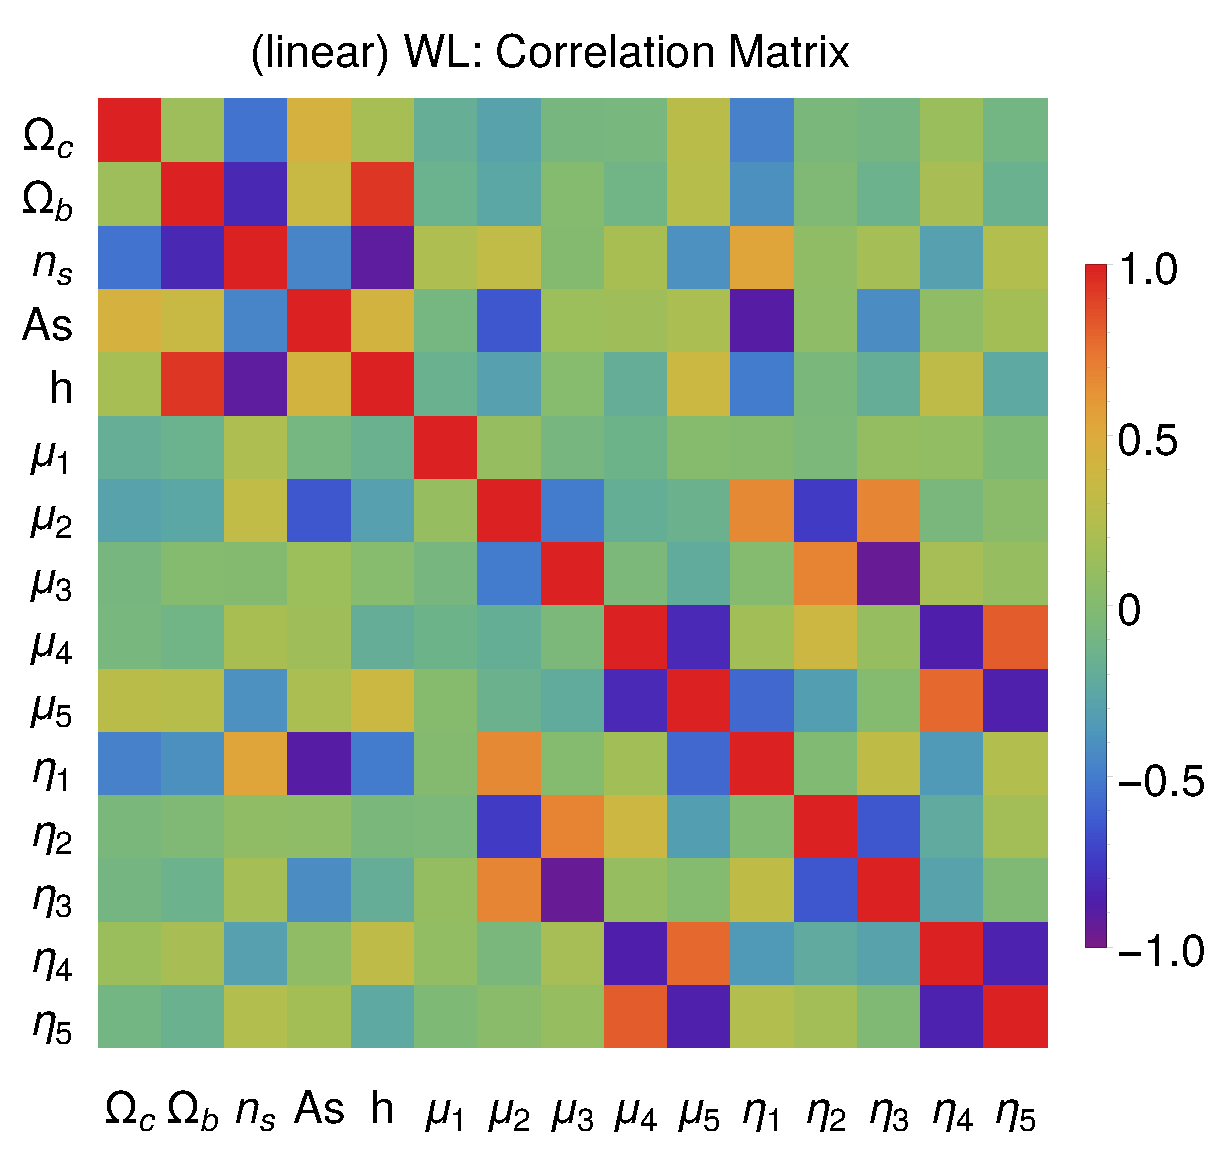
\includegraphics[width=0.47\textwidth]{Chapters/linear-nonlinear-MG-forecasts/figures/Decorrelations-WL/correlation-full-fiducialMGBin3-Euclid-WL-linearPK-}
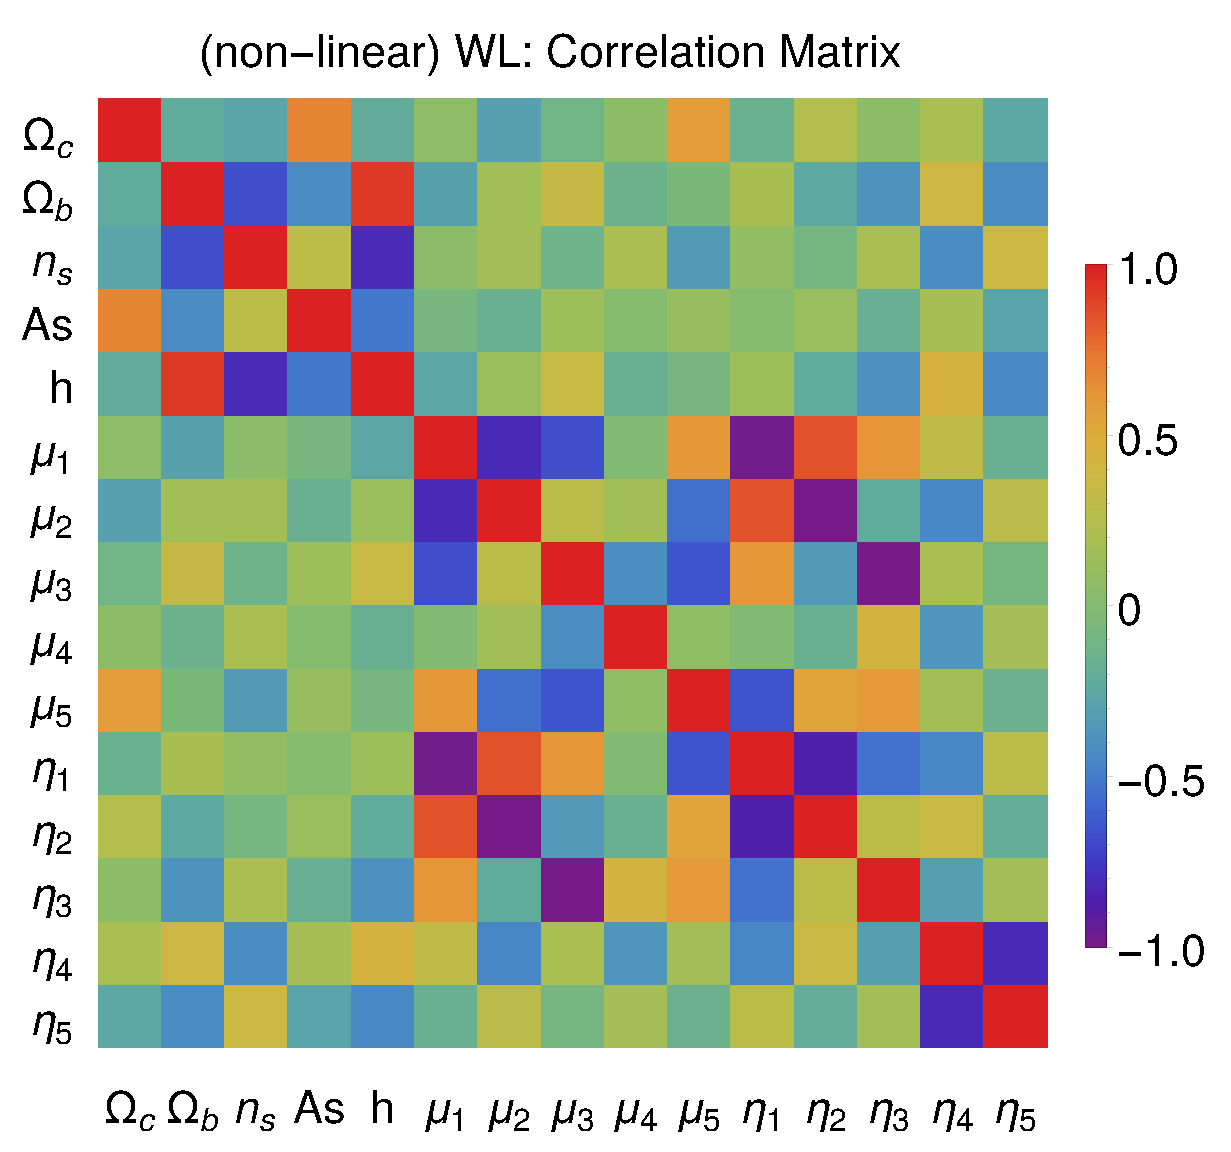
\includegraphics[width=0.47\textwidth]{Chapters/linear-nonlinear-MG-forecasts/figures/Decorrelations-WL/correlation-full-fiducialMGBin3-Euclid-WL-nonlinearPk__Zhao-}
\caption[Correlation matrices for a WL Euclid forecast.]{\label{fig:WLcorr}
Correlation matrix obtained from the covariance matrix in the MG-binning case, for a Weak Lensing Fisher Matrix forecast using Euclid
Redbook specifications. \textbf{Left panel:} linear forecasts. Strong anti-correlations are present between the $\mu_i$ and the $\eta_i$ parameters for the same value of i in {2,3,4,5}. The amplitude $\ln(10^{10}A_{s})$ parameter is mostly uncorrelated except with $\eta_1$. 
The FoC (\ref{eq:FoC}) in this case is approximately $69$.
\textbf{Right panel:} non-linear 
forecasts using the HS prescription. Here the same trend as in the linear case is present, with just subtle changes. 
The FoC in this case is about $32$, meaning that the variables are indeed less correlated than in the linear case. 
The parameter $\ln(10^{10}A_{s})$ is effectively not correlated to other parameters, 
and the anti-correlation of $\mu_{i}$ and the $\eta_{i}$ for the same value of the index i is present in the first three bins. 
The anti-correlation between these two sets of parameters
is expected, since WL is sensitive to the Weyl potential $\Sigma$, which is a product of $\mu$ and $\eta$.}
\end{figure}

\Cref{tab:errors-all-MGBin3} shows the corresponding 1$\sigma$ marginalized errors on $\ln{(10^{10}A_s)}$
and on the $\mu_i$ and $\eta_i$, both in the linear and 
non-linear cases for a Euclid Redbook WL survey. 
As in the case of GC, linear WL cannot constrain alone any of the amplitudes of 
the Modified Gravity parameters $\mu_i$ and $\eta_i$ for any redshift bin. 
Being able to include non-linear scales improves constraints on the amplitude $\ln(10^{10}A_{s})$ by a factor 100. 
The 1$\sigma$ errors on $\mu_{i}$ and $\eta_{i}$ 
improve up to one order of magnitude, with the FoM increasing by 17 nits, although remaining quite unconstraining for Modified Gravity parameters in all redshift bins.
Notice, however, that the 1$\sigma$ error on $\mu_1$ from WL in the linear case is slightly smaller than in the non-linear case.
This can be attributed to the fact that in the linear case, $\mu_1$ is uncorrelated to any other parameter, as 
shown in figure \ref{fig:WLcorr} and on that specific bin (0 < z < 0.5) non-linearities don't seem to improve the constraints on this parameter.




\subsection{Combining Euclid Galaxy Clustering and Weak Lensing, with \planck\ data \label{sub:Combined-GC-WL-Planck-Binned}}


The combination of Galaxy Clustering and Weak Lensing is expected to be very powerful for 
Modified Gravity parameters as they measure two different combinations of $\mu$ and $\eta$, 
thus breaking their degeneracy as illustrated in  \cref{fig:DE+Planck-ellipses-mu-sig-eta}. 
This is shown in \cref{tab:errors-all-MGBin3}, where the sensitivity drastically increases with respect to the two separate probes, 
especially in the low redshifts bins $(0.<z<1.5)$, where the lensing signal is dominant. 
Adding non-linearities further doubles the FoM. The \planck\ 
data constrains mostly the standard $\lcdm$ parameters and has only a limited ability to constrain the MG sector. 
However, the additional information breaks parameter degeneracies and in this way significantly decreases
the uncertainties on all parameters, so that the linear GC+WL+{\it Planck} is comparable to the non-linear GC+WL. 
Also, quantitatively, the correlation among parameters is reduced by combining GC+WL with \planck\ data. The FoC in this case is of $\approx 22$.
We also see in Table \ref{tab:errors-all-MGBin3} that the differences between the non-linear prescription
adopted here (nl-HS) and a straightforward application of Halofit to the MG case (nl-Halofit) is not
very large. We will investigate further the impact of the parameters used in the non-linear prescription in section \ref{sub:Testing-the-effect-of-Zhao}.

\section{Decorrelation of covariance matrices and the Zero-phase Component Analysis \label{sec:Decorrelation-of-covariance}}

In the previous subsections we highlighted how the MG parameters and the 
amplitude of the primordial power spectrum exhibit significant correlations and showed how including non-linearities helps to decorrelate them. Even without including non-linearities, however, it is interesting to investigate how we can completely decorrelate the parameters, identifying in this way those parameter combinations which are best constrained by data.

Given again a \emph{d-dimensional} vector
$p$ of random variables (our originally correlated parameters), we can calculate its covariance matrix $\mathbf C$ defined in Eqn.\ (\ref{eq:covariance_def}). The process of decorrelation is the process of making the matrix $\mathbf C$ 
a diagonal matrix.

Let us define some important identities. The covariance
matrix can be decomposed in its eigenvalues (the elements of a diagonal matrix $\Lambda$) and eigenvectors
(the rows of an orthogonal matrix $U$).
\begin{equation}
\mathbf C=U\Lambda U^{T} \quad \Leftrightarrow \quad 
\mathbf F=U\Lambda^{-1}U^{T} \,\,\, ,
\label{eq:eigensystemofC}
\end{equation}
where $\mathbf F$ is the Fisher Matrix.

It is possible to show that applying a transformation matrix $W$ to the $p$ parameter vector, thus obtaining a new vector of variables $q=Wp$, the covariance matrix of the transformed vector $q$ is whitened (i.e. it is the identity matrix, and whitening is defined as the process
of converting the covariance matrix into an identity matrix)
\begin{align}
\mathbf {\tilde{C}} & =W\langle\Delta\hat{p}\Delta\hat{p}^{T}\rangle W^{T} =\langle\Delta\hat{q}\Delta\hat{q}^{T}\rangle \label{eq:Cwhitened}\\
 & = \mathbbm{1} \,\,\, . \nonumber
\end{align} 
This means that the transformed $q$ parameters are decorrelated, since their correlation matrix is diagonal. The choice of $W$ 
is not unique as several  possibilities
exist; we focus on a particular choice in the rest of the chapter referred to as Zero-phase Component Analysis (ZCA, first 
introduced by \cite{Bell19973327} in the context of image processing), but we show
two other possible choices and their effect on the analysis in Appendix
\ref{sec:appdec}.

Zero-phase Component Analysis (sometimes also called Mahalanobis transformation \cite{kessy_optimal_2015}) is a specific choice of decorrelation method that 
minimizes the squared norm of the difference between the $q_i$
and the $p_i$ vector $\|\vec{p}-\vec{q}\|$, under the constraint that the vector $\vec{q}$ should be uncorrelated \cite{kessy_optimal_2015}. 
In this way the uncorrelated variables $q$ will be as close 
as possible to the original variables $p$ in a least squares sense. 
This is achieved by using the $W$ matrix:
\begin{equation}
W \equiv F^{1/2} \,\,\, .
\end{equation}
Then in this case, the covariance matrix is whitened, by following Eqn.\ (\ref{eq:Cwhitened}):
\begin{equation}
\tilde{C} =F^{1/2}F^{-1}F^{1/2}=\mathbbm{1} \,\,\, .
\end{equation}
In our case, since we do not want to whiten, but just decorrelate the covariance matrix,
we renormalize the $W$ matrix by multiplying with a diagonal matrix $N_{jj}\equiv\sum_j(W_{ij}^{-2})$, such that the sum of the square of the 
elements on each row of the new weighting matrix 
$\tilde{W} \equiv N W$, is equal to unity; therefore the final
transformed covariance is still diagonal but is not the identity matrix: 
\begin{equation}
\tilde{C}=\tilde{W}C\tilde{W}=N^{2} \mathbbm{1} \label{eq:Ctilde-decor}
\end{equation}
and at the same time we ensure that 
the vector of new variables $q_i$ will have the same norm as the old vector of variables $p_i$.

\subsection{ZCA for Galaxy Clustering \label{subsub:ZCA-GC}}


From Fig.\ \ref{fig:GCcorr} we can see that the correlations are present in sub-blocks, one for 
the standard $\lcdm$ parameters and another one for the Modified Gravity parameters. The exception lies in the linear case
where $\lAs \equiv \ln{(10^{10}A_s)}$ is strongly anti-correlated with all the $\mu_i$ and positively correlated with the $\eta_i$. 
To use a more objective criterion, we choose the $10\times 10$ block of MG parameters $\mu_i$ and $\eta_i$ with parameter indices 6 to 15, and only add to this block a $\lcdm$ parameter with index $a$
if the following condition is satisfied:
\[
 \sum_{i=6}^{i=15}(P_{ai})^2 \geq 1
\]
where the index $a$ corresponds to one of the first five standard parameters. For Galaxy Clustering, the only index satisfying this condition is $a=4$ in the linear case, corresponding to $\lAs \equiv \ln{(10^{10}A_s)}$: i.e. the standard parameter corresponding to the amplitude is, as said, degenerate with Modified Gravity parameters $\mu_i$ and $\eta_i$.
In the non-linear case no parameter satisfies this condition (because, as we have seen, non-linearities are able to eliminate correlation with the amplitude), but for consistency we will use the same vector of 11 parameters
$p_i = \left\{ \lAs, \mu_i, \eta_i \right\}$ for our decorrelation procedure.
Therefore we will also have 11 transformed uncorrelated $q_i$ parameters, function of the original $p_i$ parameters, in all the cases presented below. 


Figure \ref{fig:Wmat-ZCA-GC} shows the coefficients that relate the 
$q_i$ parameters to the original $p_i$ ones, in the linear (left panel) and the non-linear (right panel) cases. The explicit coefficients are shown in Appendix D of the publication \cite{casas_linear_2017}.
%\ref{tab:Wcoeff-lin-GC} and \ref{tab:Wcoeff-nlHS-GC} of Appendix \ref{sec:Wmatrices}.
We plot in figure \ref{fig:GCbinerrs} a comparison between the 1$\sigma$ errors on the primary parameters $p_i$ 
(represented by circles connected with dark green dashed lines) and the decorrelated parameters $q_i$ 
(represented by squares connected with orange solid lines). 
In the linear case (left panel), we can see that the errors on the $q_i$ parameters are 2 orders of magnitude 
better than the errors on the $p_i$ parameters. In the non-linear case (right panel) the improvement is of at most 1 order of magnitude 
and that for a completely decorrelated parameter like $\lAs$, 
the error on its corresponding $q_i$ is exactly the same. 
This shows that a decorrelation procedure is still worth to do, even when including the non-linear regime, 
even if the degeneracy with the amplitude is already completely broken thanks to the non-linear prescription.
The fact that the curve of 1$\sigma$ errors for the $q_i$ follows the same pattern as the curve for the $p_i$ errors, 
is due to the fact that we have used a ZCA decomposition 
(see section \ref{sec:Decorrelation-of-covariance}) and therefore the $q_i$ are as similar as possible to the $p_i$.


\begin{figure}[htbp]
	\centering
	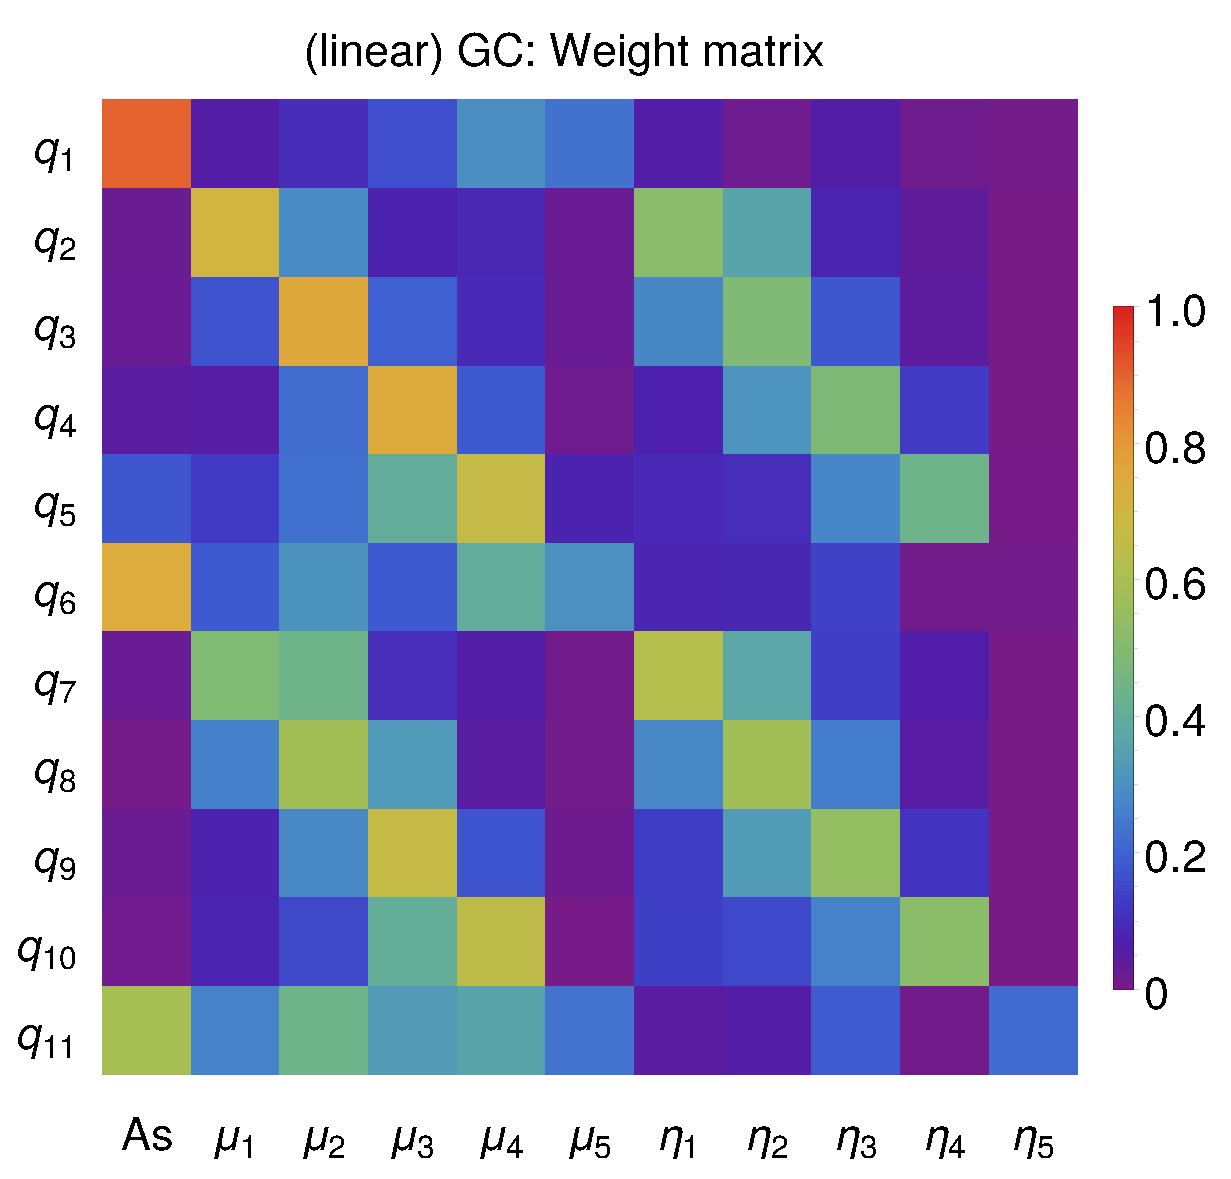
\includegraphics[width=0.47\textwidth]{Chapters/linear-nonlinear-MG-forecasts/figures/Decorrelations-GC/Weight_Matrix_ZCA_SquareNorm--_fiducialMGBin3_Euclid_GC_linearPK_}
	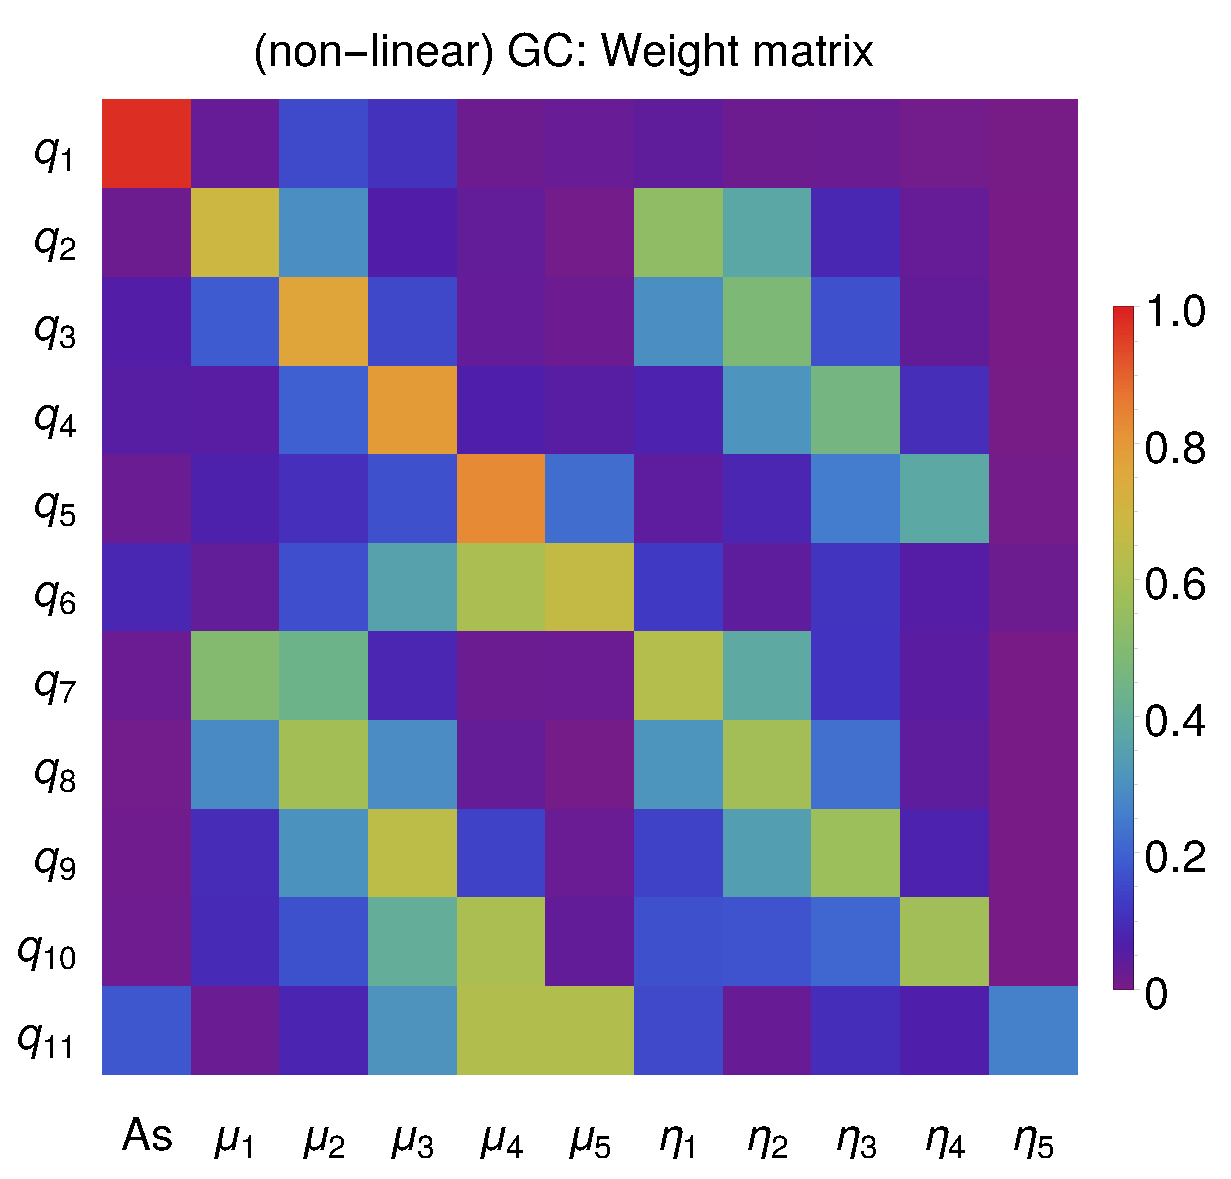
\includegraphics[width=0.47\textwidth]{Chapters/linear-nonlinear-MG-forecasts/figures/Decorrelations-GC/Weight_Matrix_ZCA_SquareNorm--_fiducialMGBin3_Euclid_GC_nonlinearPk__Zhao_}
	\caption[Weight matrix for ZCA decorrelation in a Euclid GC case.]{\label{fig:Wmat-ZCA-GC}
	Entries of the matrix $W$ that relates the $q_i$ parameters to the original $p_i$ ones, after applying the ZCA decorrelation of the covariance matrix in the linear and non-linear GC cases. This matrix shows for each new variable $q_i$ on the vertical axis, the coefficients of the linear combination of parameters $\mu_i$, $\eta_i$ and $A_s$ that give rise to that variable $q_i$. The red (blue) colors, indicate a large (small) contribution of the respective variable on the horizontal axis. \textbf{Left panel:} linear forecast for Euclid Redbook specifications.
\textbf{Right panel:} non-linear forecast for Euclid Redbook specifications, using the HS prescription.
In both cases one can observe that most $q_i$ parameters have only small or negligible contributions from $\mu_5$  and $\eta_5$, which are found to be the less constrained bins.
    }
\end{figure}


\begin{figure}[htbp]
\centering{}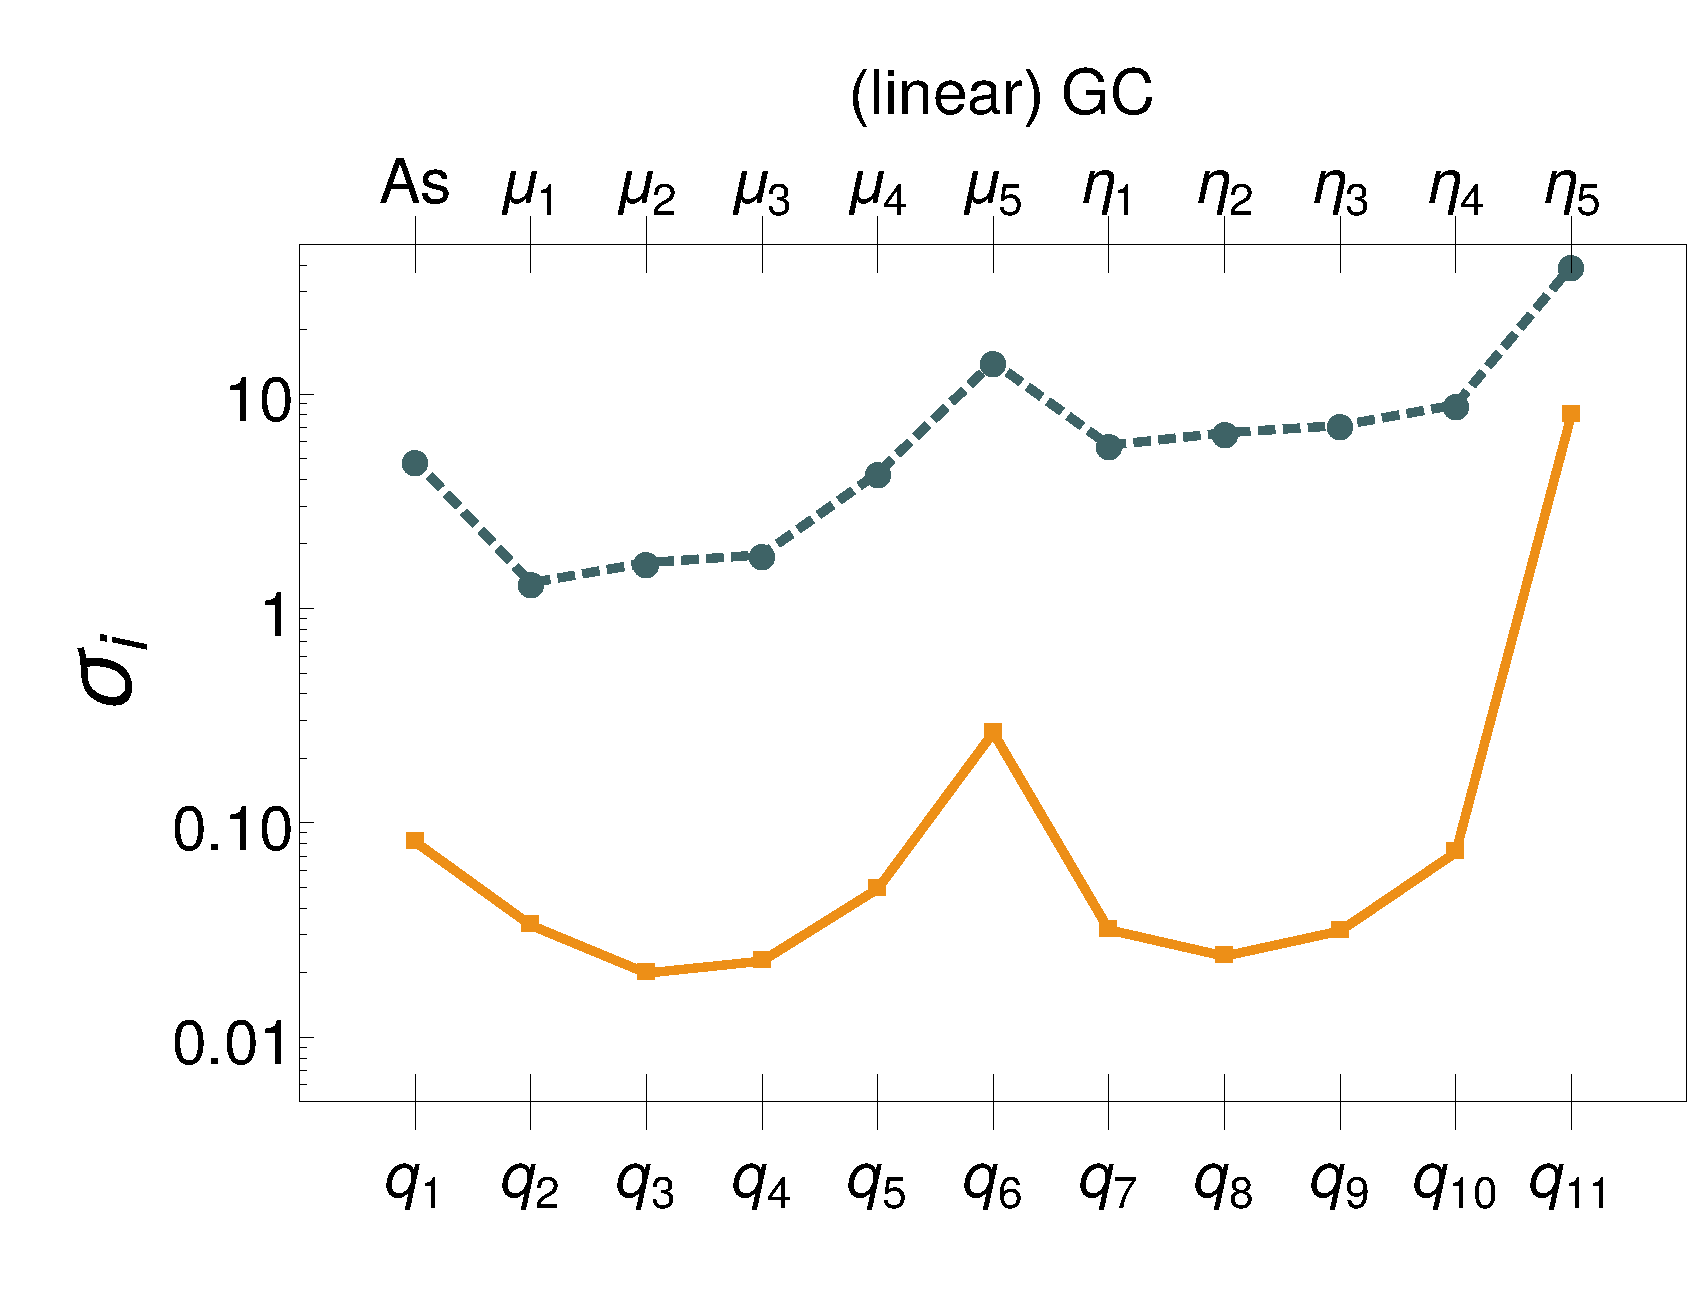
\includegraphics[width=0.47\linewidth]{Chapters/linear-nonlinear-MG-forecasts/figures/Decorrelations-GC/Errors_at_par_index_i--_ZCA_SquareNorm--fiducialMGBin3_Euclid_GC_linearPK_}
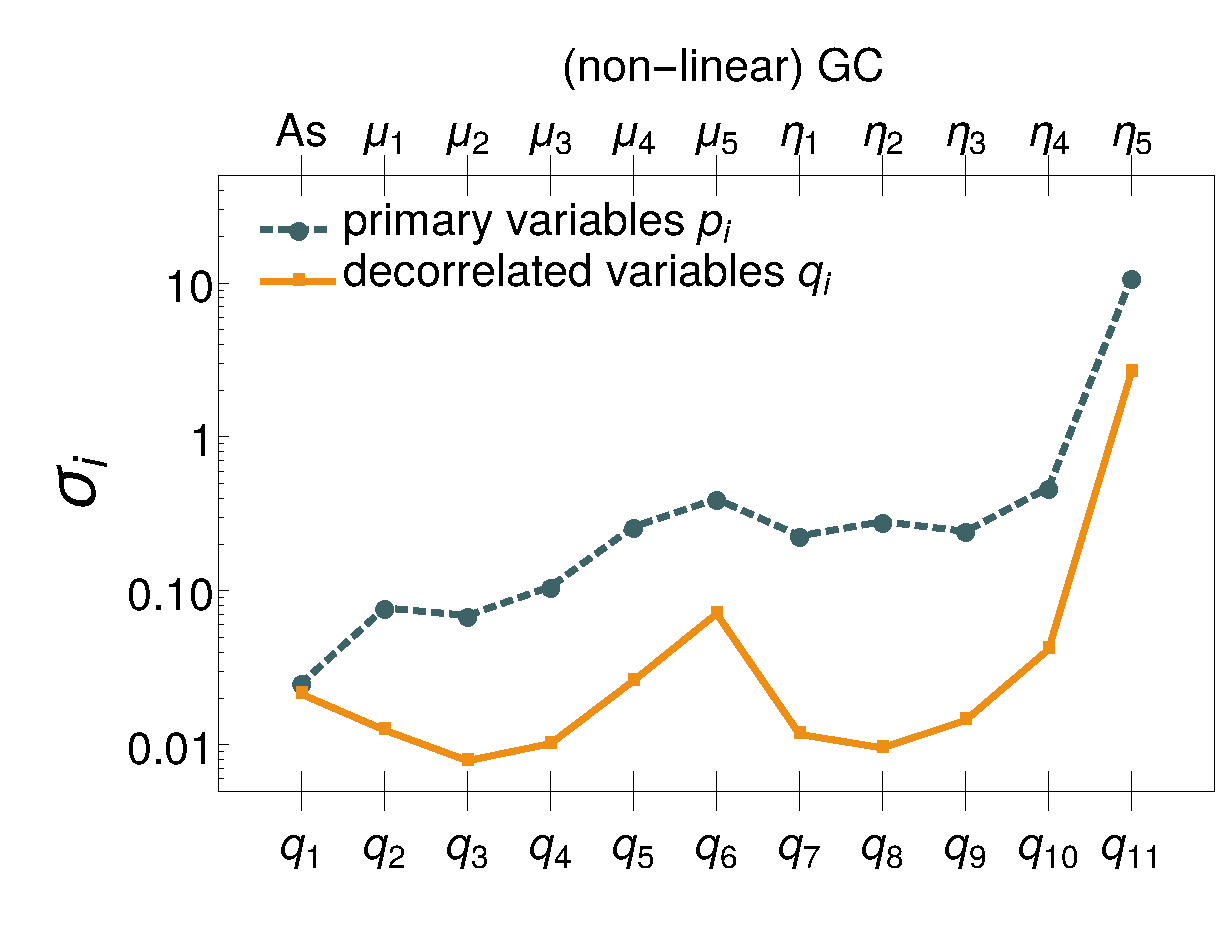
\includegraphics[width=0.47\linewidth]{Chapters/linear-nonlinear-MG-forecasts/figures/Decorrelations-GC/Errors_at_par_index_i--_ZCA_SquareNorm--fiducialMGBin3_Euclid_GC_nonlinearPk__Zhao_}
\caption[1$\sigma$ forecasted errors on the primary and decorrelated parameters for Euclid GC.]{\label{fig:GCbinerrs}
Results for a Euclid Redbook GC survey, with redshift-binned parameters, before and after applying the ZCA decorrelation.
Each panel shows the 1$\sigma$ fully marginalized errors on the primary parameters $p_i$ (green dashed
lines), and the 1$\sigma$ errors on the decorrelated 
parameters $q_i$ (orange solid lines). \textbf{Left: } linear forecasts,
performed using linear power spectra up to a maximum wavenumber $k_{\rm max}=0.15$h/Mpc.
\textbf{Right: }non-linear forecasts using non-linear spectra with the HS prescription up to a maximum wavenumber $k_{\rm max}=0.5$h/Mpc.
In the linear case, the errors on the decorrelated $q_i$ parameters are about 2 orders of magnitude smaller than for the primary parameters, 
while in the non-linear HS case, the improvement in the errors is of one order of magnitude. This means that applying a decorrelation procedure is worth even when non-linearities are considered.
In both cases for GC, the least constrained parameters are $\mu_5$ and $\eta_5$, corresponding to $2.0 < z < 2.5$.}
\end{figure}

\begin{figure}[htbp]
	\centering{}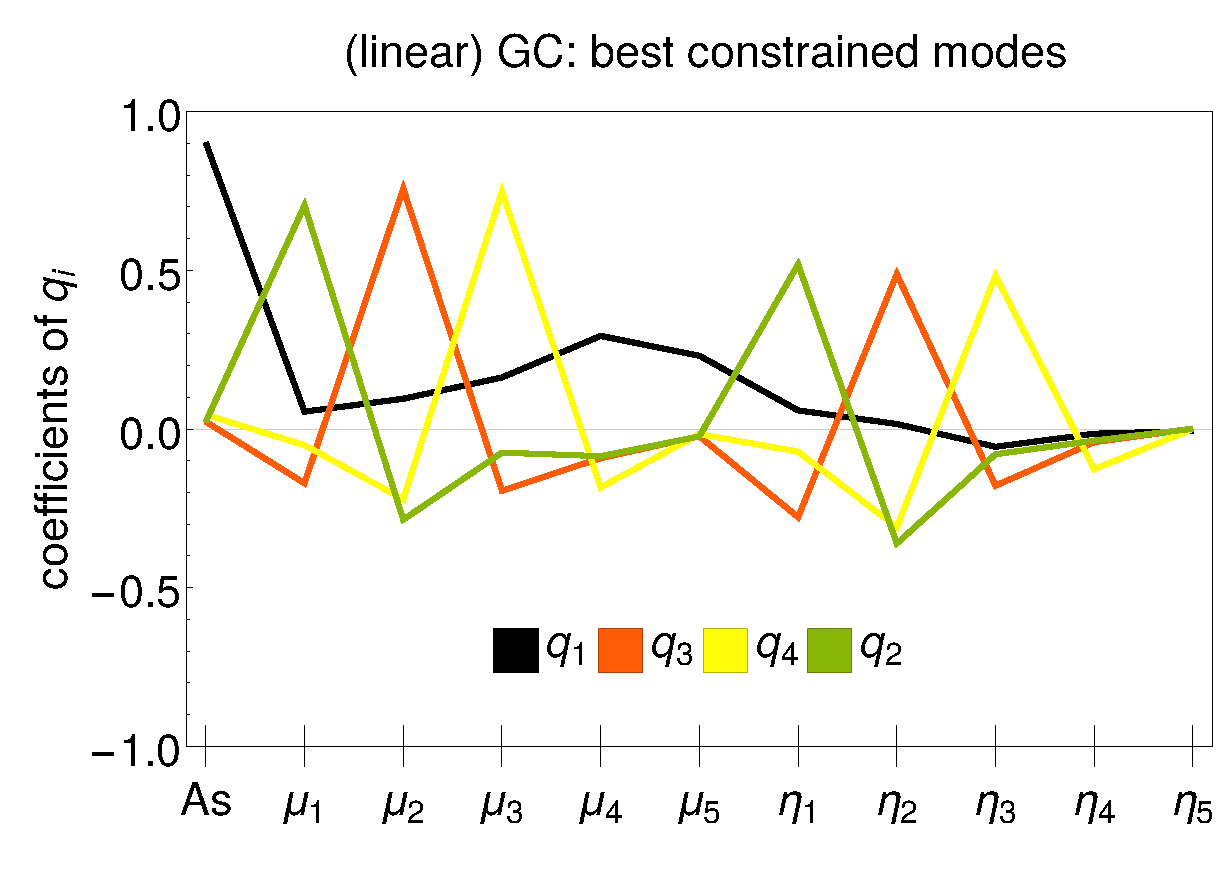
\includegraphics[width=0.47\linewidth]{Chapters/linear-nonlinear-MG-forecasts/figures/Decorrelations-GC/linear_GC--_best_constrained_modes-Errors_on_q_ZCA_SquareNorm--_fiducialMGBin3_Euclid_GC_linearPK_}
	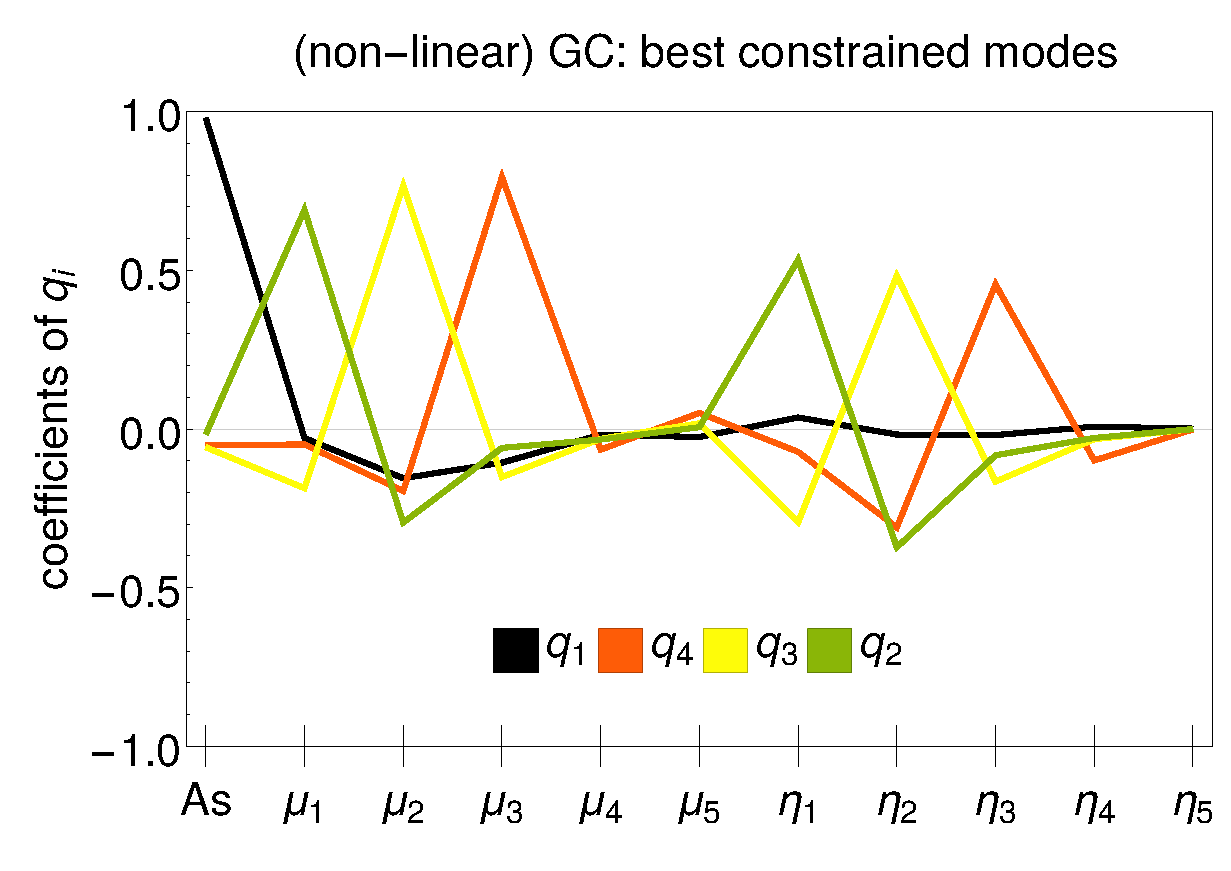
\includegraphics[width=0.47\linewidth]{Chapters/linear-nonlinear-MG-forecasts/figures/Decorrelations-GC/non-linear_GC--_best_constrained_modes-Errors_on_q_ZCA_SquareNorm--_fiducialMGBin3_Euclid_GC_nonlinearPk__Zhao_}
	\caption[Best constrained modes for Euclid GC applying ZCA.]{\label{fig:GCbestconst}
Best constrained modes for a Euclid Redbook GC survey, with $\mu$ and $\eta$ binned in redshift, 
after transforming into uncorrelated $q$ parameters via ZCA. 
Each of the four best constrained parameters $q_i$, shown in the panels, 
is a linear combination of the primary parameters $p_i$. The $q_i$ in the legends are ordered from left to right, from the best constrained to the least constrained.}
\end{figure}


We are interested in finding the best combination of primary parameters $p_i$ giving rise
to the best constrained uncorrelated parameters $q_i$. In order to find the errors 
on the parameters $q_i$, we need to look at the diagonal of the decorrelated covariance matrix $\mathbf{\tilde{C}}$ expressed in \cref{eq:Ctilde-decor} and 
identify the $q_i$ parameters with the smallest relative errors ($\sigma_{q_i}/q_i$): we find than in the linear GC case, the best 
constrained combinations of primary parameters (ordered from most to least constrained) are given approximately by:

\begin{equation} \label{eq:bestCombined-GClin}
\begin{aligned}
	q_1  &= +0.9 \lAs  +  0.32 \mu_4 \\
	q_3  &= +0.75\mu_2 - 0.29\eta_1 + 0.50 \eta_2\\
	q_4  &= -0.25\mu_2 + 0.74\mu_3  - 0.32 \eta_2 + 0.49 \eta_3 \\
	q_2  &= +0.70\mu_1 - 0.30\mu_2  + 0.52 \eta_1 - 0.36 \eta_2 \,\,\, .
\end{aligned}
\end{equation}
In contrast, for the non-linear GC case, the parameter $\lAs \equiv \ln{(10^{10}A_s)}$ is not correlated to any other, and therefore it 
is well constrained on its own. The best 4 constrained parameters (ordered from most to least constrained) in the non-linear case, are:
\begin{equation} \label{eq:bestCombined-GCnonlin}
\begin{aligned}
	q_1  &= +0.99\lAs \\
	q_4  &= -0.28\mu_2 + 0.76\mu_3 -0.33 \eta_2 + 0.47 \eta_3\\
	q_3  &= +0.73\mu_2 -0.32 \eta_1 + 0.49 \eta_2\\
	q_2  &= +0.68\mu_1 -0.35\mu_2 + 0.52 \eta_1 -0.37 \eta_2 \,\,\, .
\end{aligned}
\end{equation}
The best constrained decorrelated parameters $q_i$ for a Euclid GC survey, 
expressed in the set of Equations (\ref{eq:bestCombined-GClin}) (linear) and (\ref{eq:bestCombined-GCnonlin}) (non-linear HS), 
can be seen graphically in Fig.\ \ref{fig:GCbestconst} for the linear (left panel) 
and non-linear HS (right panel) cases respectively. 
From these combinations we see that a survey like Euclid, using GC only, will be sensitive to Modified Gravity parameters $\mu$ and $\eta$ mainly in the first three redshift bins, corresponding to a range $0. < z < 1.5$.
The complete matrix $W$ of coefficients relating the $q_i$ to the $p_i$ parameters, 
can be found in Appendix D of the publication \cite{casas_linear_2017}.


\subsection{ZCA for Weak Lensing}

We apply the same decorrelation procedure to the WL case, obtaining the $q$ vectors
shown in the weight matrix of figure \ref{fig:Wmat-ZCA-WL}.
%again reported explicitly in Tables \ref{tab:Wcoeff-lin-WL} and \ref{tab:Wcoeff-nlHS-WL}
%in Appendix \ref{sec:Wmatrices}. 

\begin{figure}[htbp]
	\centering{}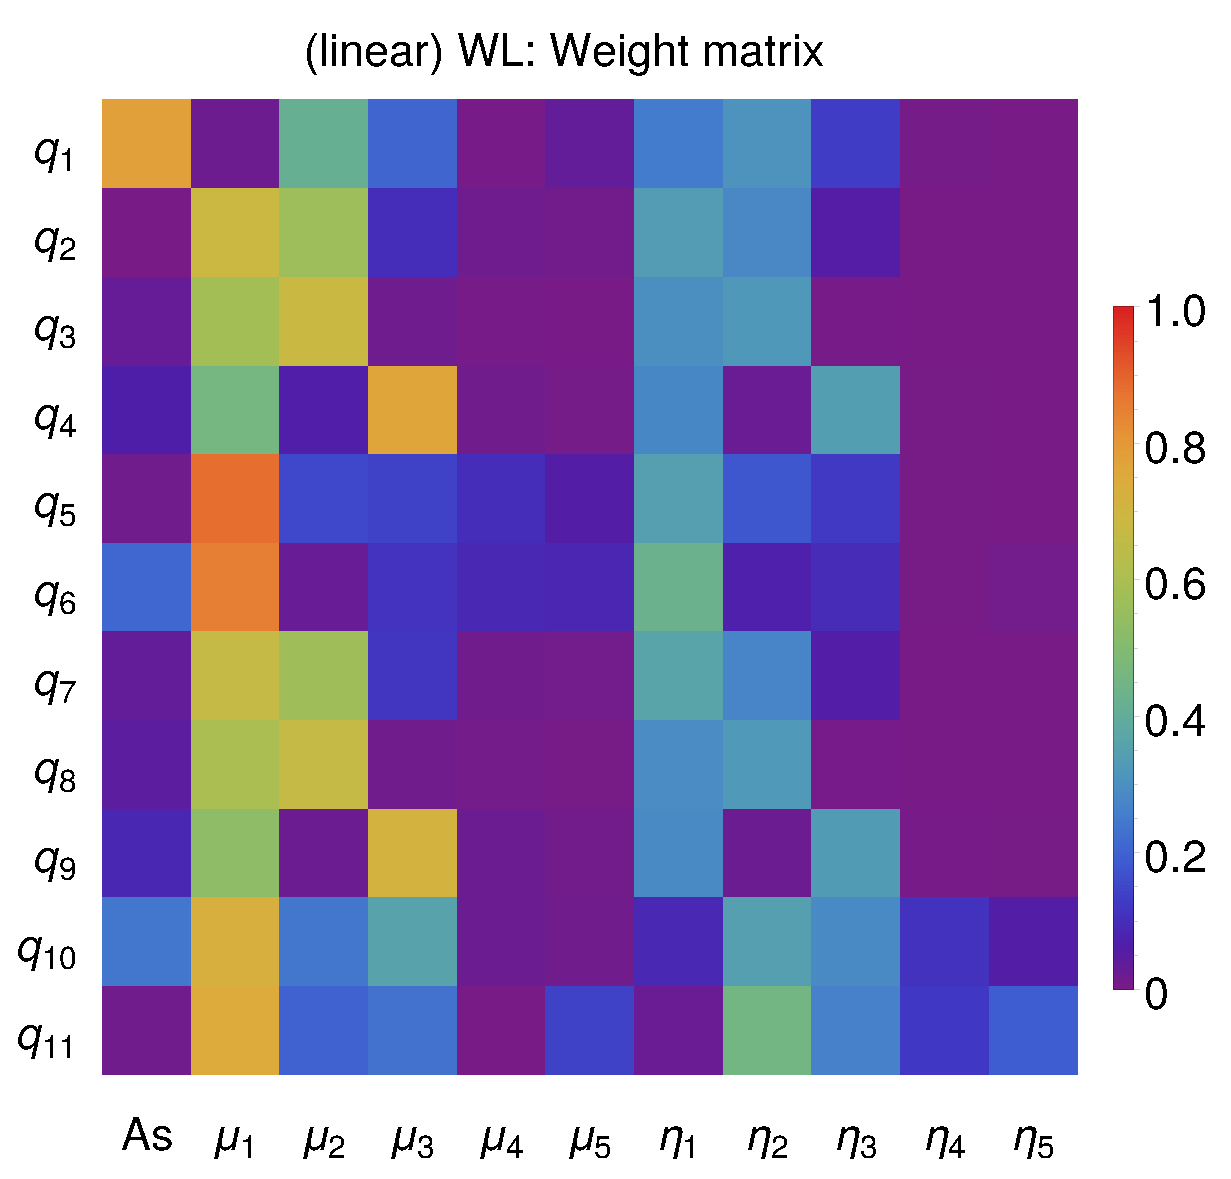
\includegraphics[width=0.47\linewidth]{Chapters/linear-nonlinear-MG-forecasts/figures/Decorrelations-WL/Weight_Matrix_ZCA_SquareNorm--_fiducialMGBin3_Euclid_WL_linearPK_}
	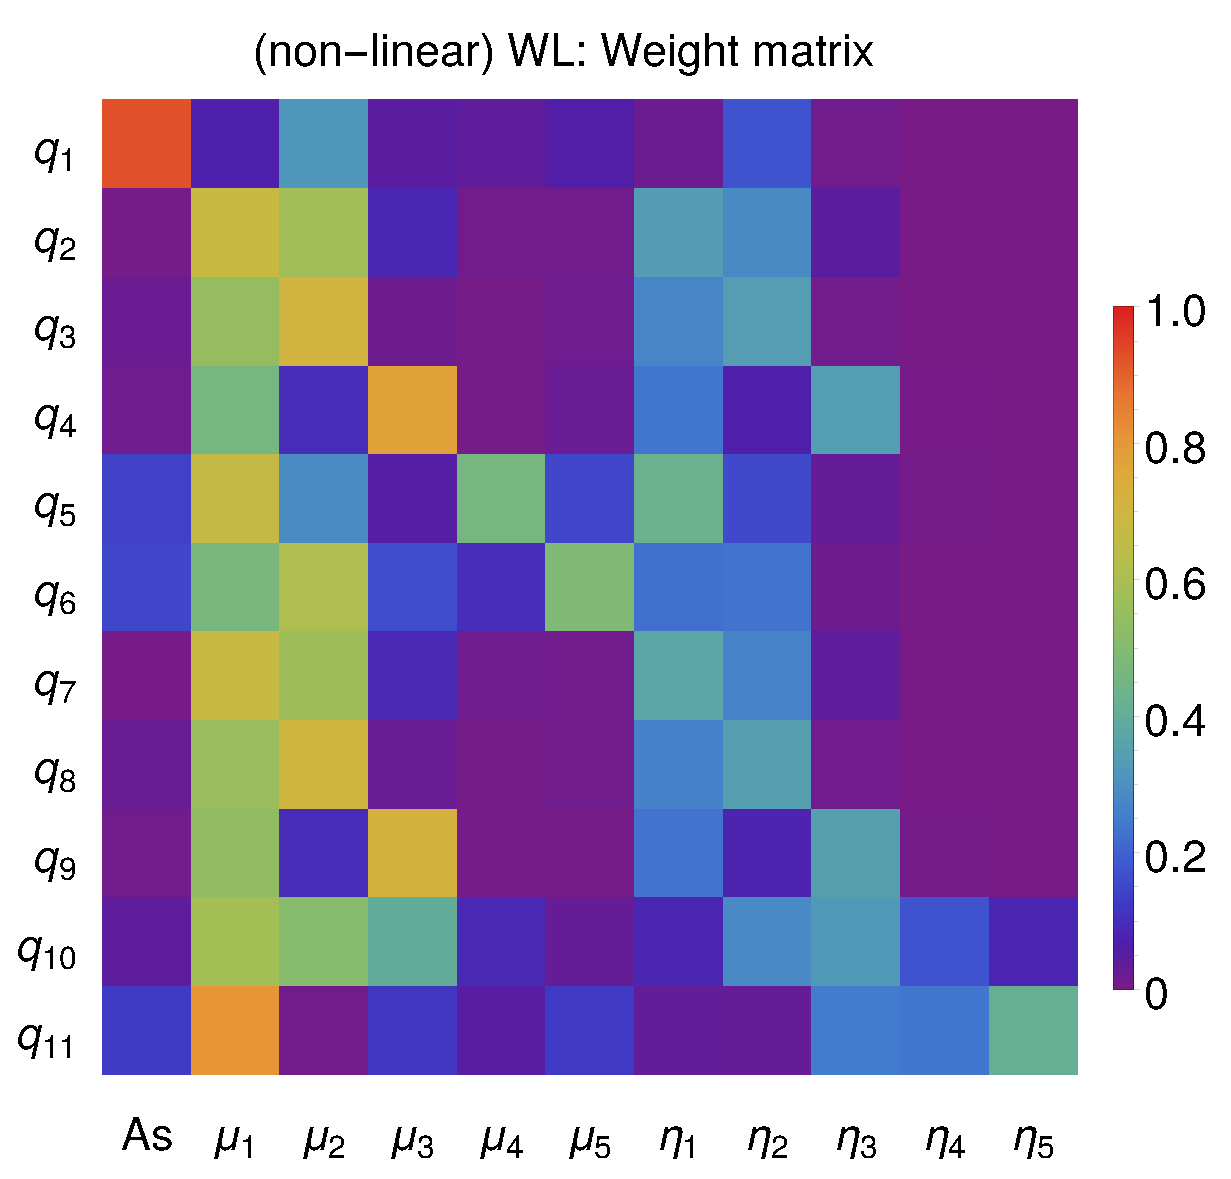
\includegraphics[width=0.47\linewidth]{Chapters/linear-nonlinear-MG-forecasts/figures/Decorrelations-WL/Weight_Matrix_ZCA_SquareNorm--_fiducialMGBin3_Euclid_WL_nonlinearPk__Zhao_}
	\caption[Weight matrix for ZCA decorrelation in a Euclid WL case.]{
Entries of the matrix $W$ that relates the $q_i$ parameters to the original $p_i$ ones, after applying the ZCA decorrelation of the covariance matrix in the linear and non-linear WL cases. This matrix shows for each new variable $q_i$ on the vertical axis, the coefficients of the linear combination of parameters $\mu_i$, $\eta_i$ and $A_s$ that give rise to that variable $q_i$. The red (blue) colors, indicate a large (small) contribution of the respective variable on the horizontal axis. \textbf{Left panel:} linear forecast for Weak Lensing Euclid Redbook specifications.
\textbf{Right panel:} non-linear forecast for Weak Lensing Euclid Redbook specifications, using the HS prescription.
As for GC, most $q_i$ parameters have only small or negligible contributions from $\mu_5$  and $\eta_5$, which are found to be the less constrained bins.
	\label{fig:Wmat-ZCA-WL}}
\end{figure}

In figure \ref{fig:WLbinerrs} we show the comparison between the errors on the primary
parameters $p_i$ and the de-correlated ones $q_i$. As for the GC case, the errors in the linear case improve by 2 orders of magnitude after applying the decorrelation procedure (left panel). In the non-linear case (right panel) the improvement is smaller, but still worth to do, especially to constrain $q_2,q_3,q_7,q_8$.

\begin{figure}[htbp]
	\centering{}\begin{center}
		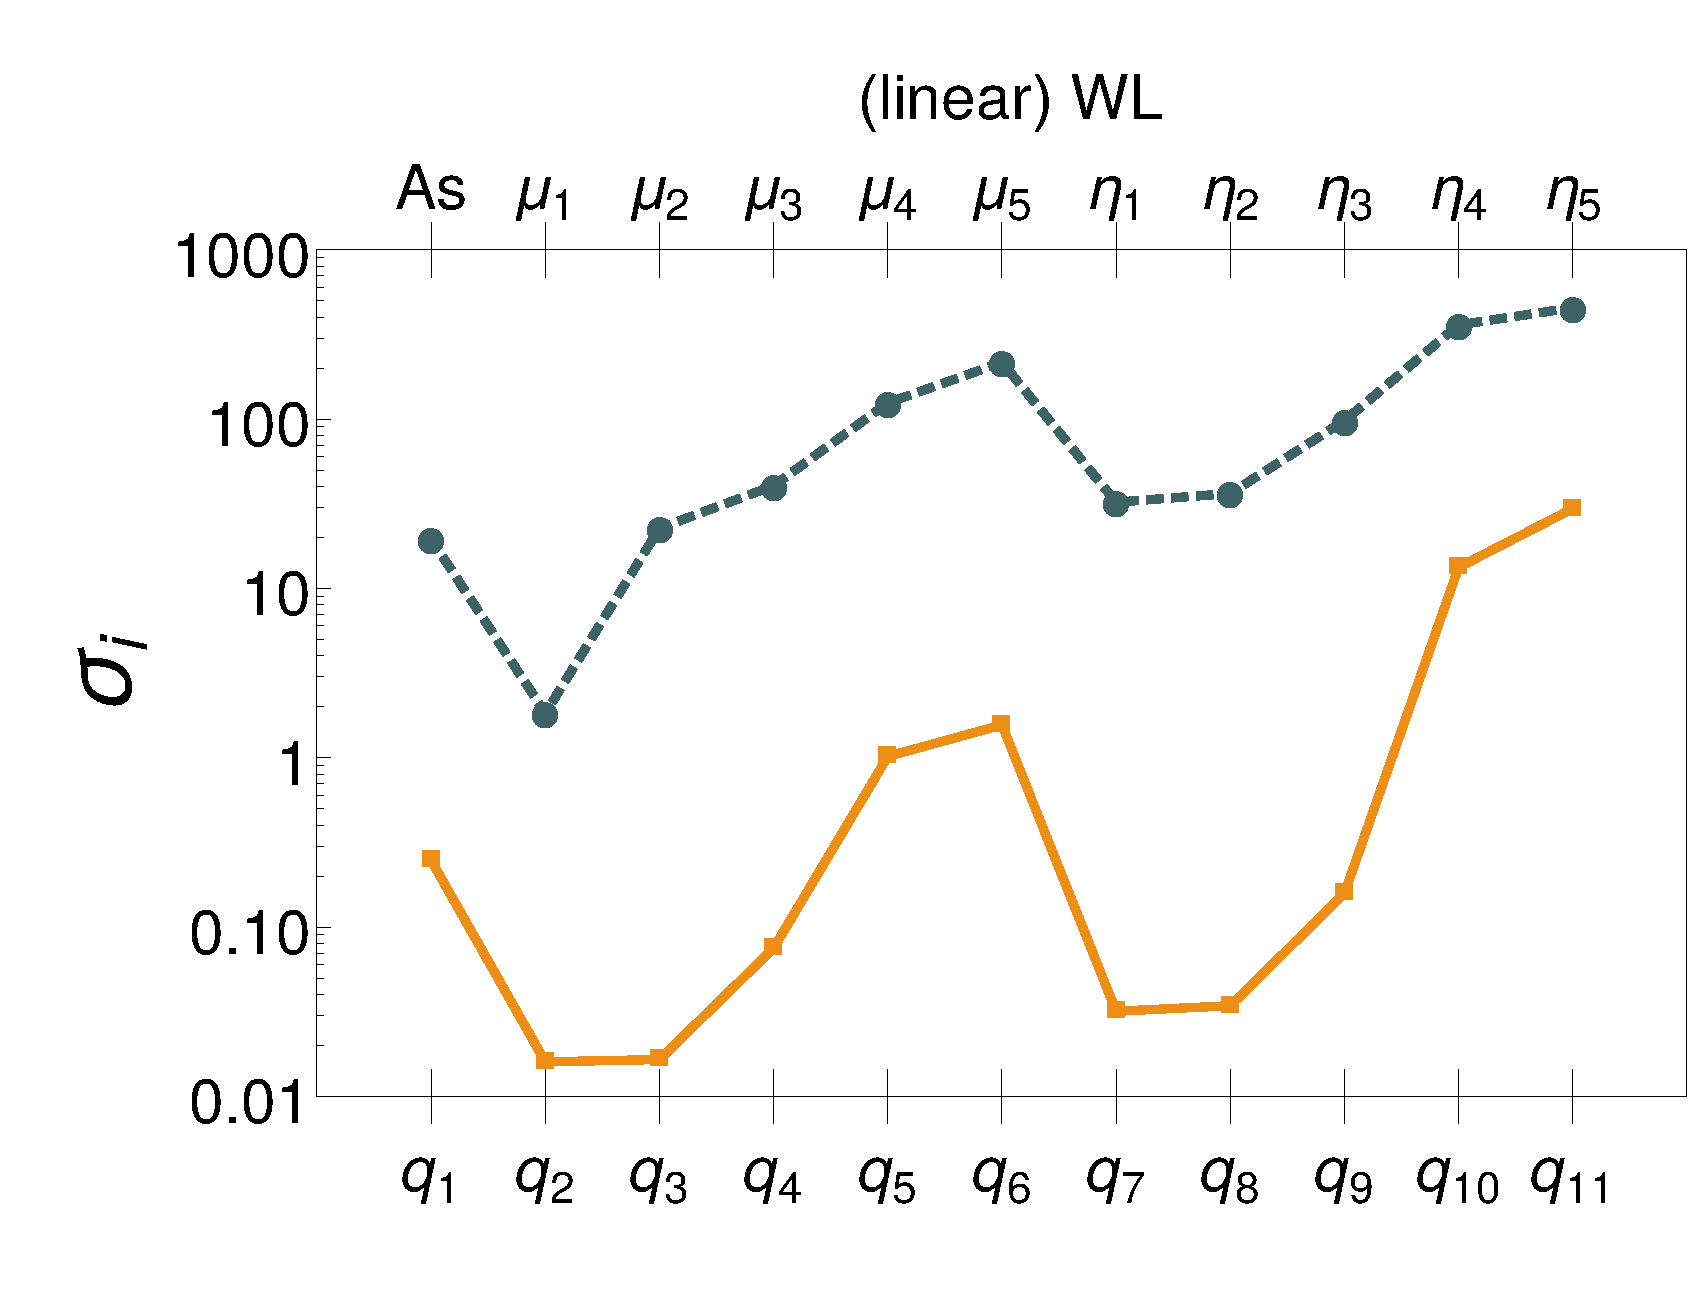
\includegraphics[width=0.47\linewidth]{Chapters/linear-nonlinear-MG-forecasts/figures/Decorrelations-WL/Errors_at_par_index_i--_ZCA_SquareNorm--fiducialMGBin3_Euclid_WL_linearPK_}
		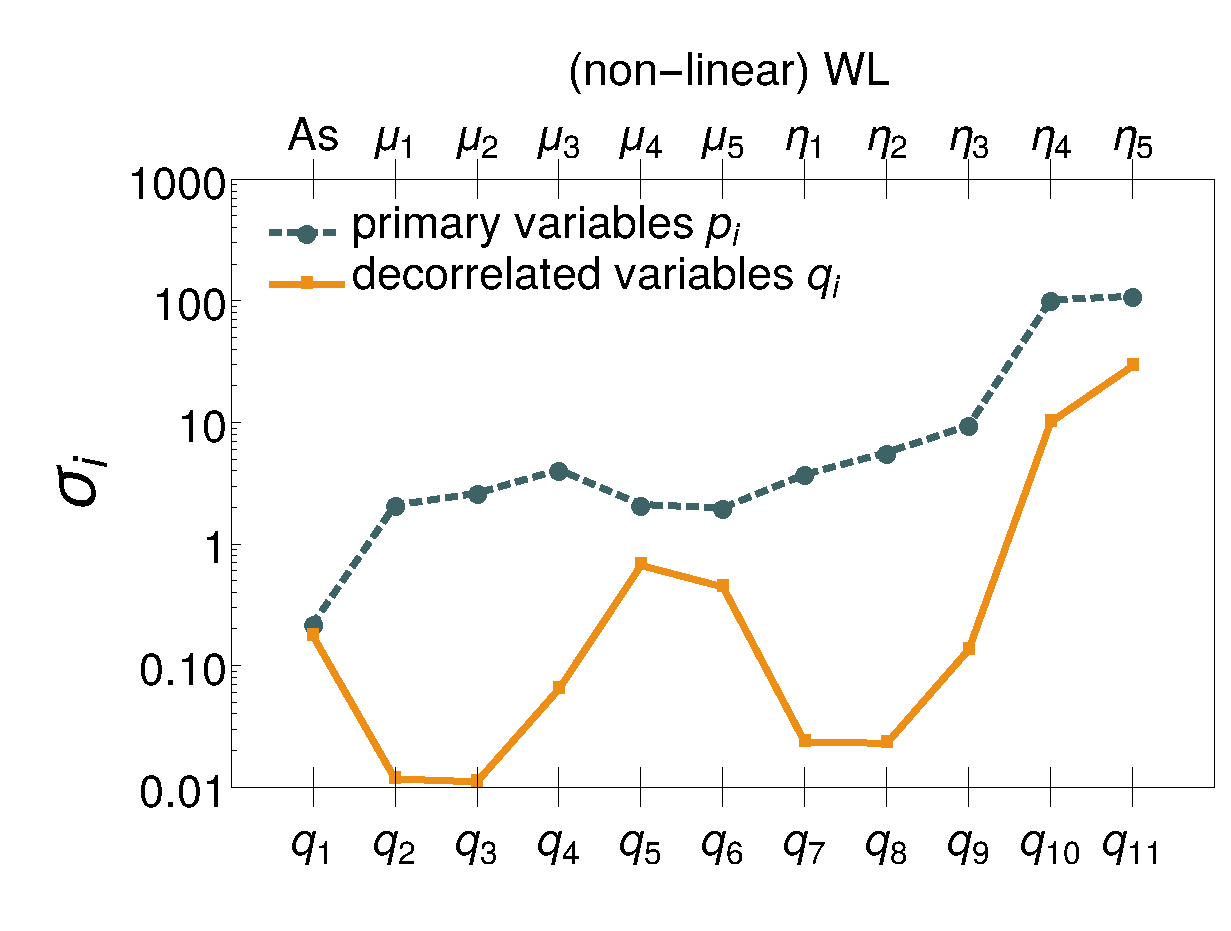
\includegraphics[width=0.47\linewidth]{Chapters/linear-nonlinear-MG-forecasts/figures/Decorrelations-WL/Errors_at_par_index_i--_ZCA_SquareNorm--fiducialMGBin3_Euclid_WL_nonlinearPk__Zhao_}
	\end{center}
	\caption[1$\sigma$ forecasted errors on the primary and decorrelated parameters for Euclid WL.]{\label{fig:WLbinerrs} 
	Results for a Euclid Redbook WL survey, with redshift-binned parameters, 
	before and after applying the ZCA decorrelation.
	Each panel shows the 1$\sigma$ fully marginalized errors on the primary parameters $p_i$ (green dashed
		lines), and the 1$\sigma$ errors on the decorrelated
		parameters $q_i$ (orange solid lines). \textbf{Left: }Linear forecasts,
		performed with an $\ell_{\rm max}=1000$ and linear matter power spectra.
		\textbf{Right: }Non-linear forecasts using the non-linear spectra with the HS prescription, up to an $\ell_{\rm max}=5000$.
		The errors in the non-linear HS case, are about 1 order of magnitude smaller than in the linear case. 
		For the best constrained $q_i$ parameters, the 
		decorrelated errors are up to 2 orders of magnitude smaller than the corresponding fully marginalized parameters on the parameters $p_i$.}
\end{figure}


More generally, as we did for the GC case in the previous section, we look for the $q_i$ 
parameters with the smallest relative errors ($\sigma_{q_i}/q_i$) and find in the linear WL case, that the best 
constrained combinations (ordered from most to least constrained) of primary parameters are given approximately by: 

\begin{equation} \label{eq:bestCombined-WLlin}
\begin{aligned}
	q_1  &= +0.76\lAs + 0.48 \mu_2 + 0.33\eta_2 \\
	q_3  &= -0.59\mu_1 + 0.67 \mu_2 - 0.30\eta_1 + 0.32 \eta_2\\
	q_7  &= +0.65\mu_1 - 0.60 \mu_2 + 0.36\eta_1 - 0.28 \eta_2\\
	q_2  &= +0.67\mu_1 - 0.59 \mu_2 + 0.33\eta_1 - 0.29 \eta_2 \,\,\, .
\end{aligned}
\end{equation}
This means that WL in the linear case will only be able to constrain 
combinations of the first two redshift bins in $\mu$ and $\eta$ (corresponding to  $ 0. < z < 1.0 $).
This can also be observed graphically in the left panel of Figure \ref{fig:WLbestconst}.
For the non-linear WL case, the combinations remain practically the same, except for $q_1$, which will depend much more strongly on the parameter $\lAs$. The best 4 constrained parameters in this case, are (ordered from most to least constrained):
\begin{equation} \label{eq:bestCombined-WLnonlin}
\begin{aligned}
	q_3  &= -0.55\mu_1 + 0.71 \mu_2 + -0.27\eta_1 + 0.34\eta_2\\            
	q_1  &= +0.93\lAs - 0.32\mu_2 \\ 
	q_2  &= +0.67\mu_1 - 0.60 \mu_2 + 0.33\eta_1 - 0.29 \eta_2\\
	q_4  &= -0.46\mu_1 + 0.29 \mu_2 + 0.73\mu_3 + 0.31 \eta_3 \,\,\, .
\end{aligned}
\end{equation}
These combinations can also be visualized in the right panel of figure \ref{fig:WLbestconst}.
The complete matrix $W$ of coefficients relating the $q_i$ to the $p_i$ parameters, 
can be found in Appendix D of the publication \cite{casas_linear_2017}.

\begin{figure}[htbp]
	\centering{}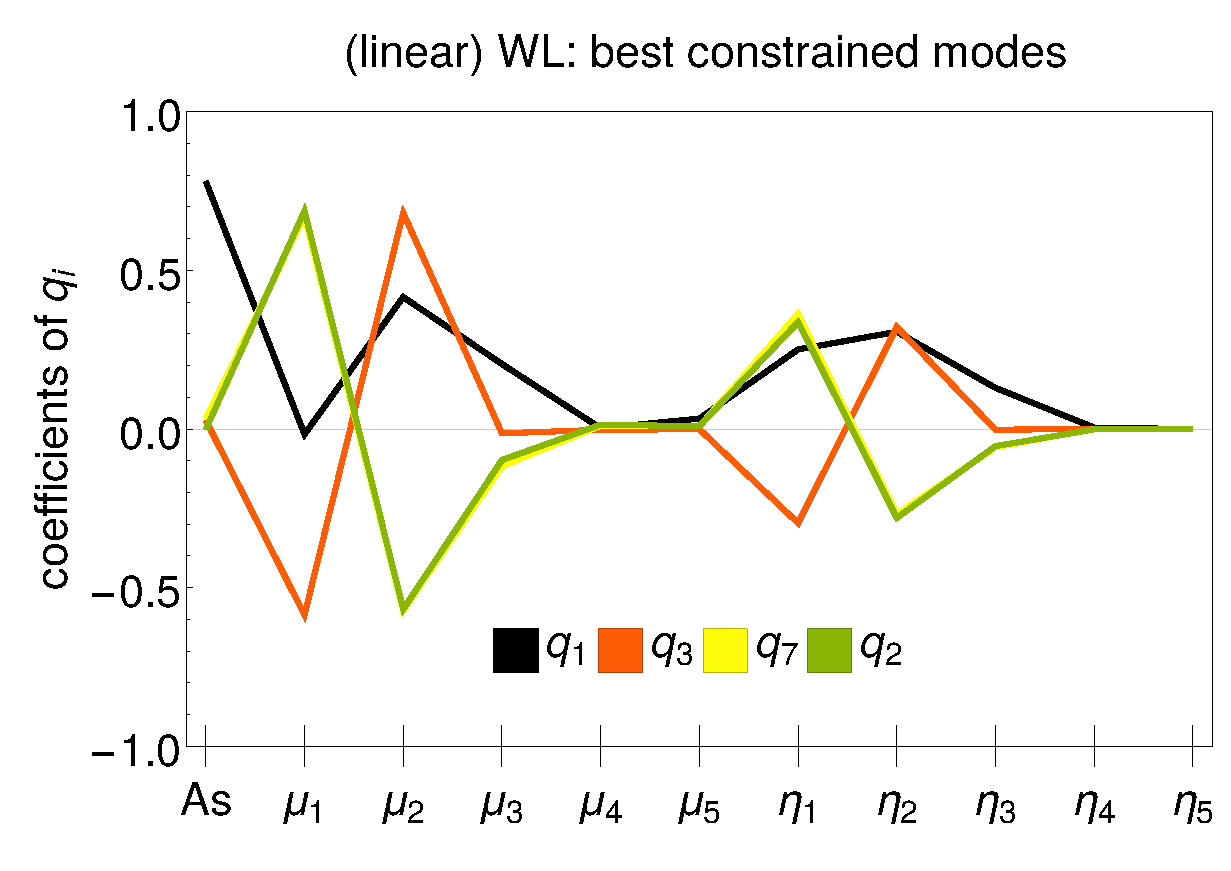
\includegraphics[width=0.47\linewidth]{Chapters/linear-nonlinear-MG-forecasts/figures/Decorrelations-WL/linear_WL--_best_constrained_modes-Errors_on_q_ZCA_SquareNorm--_fiducialMGBin3_Euclid_WL_linearPK_}
	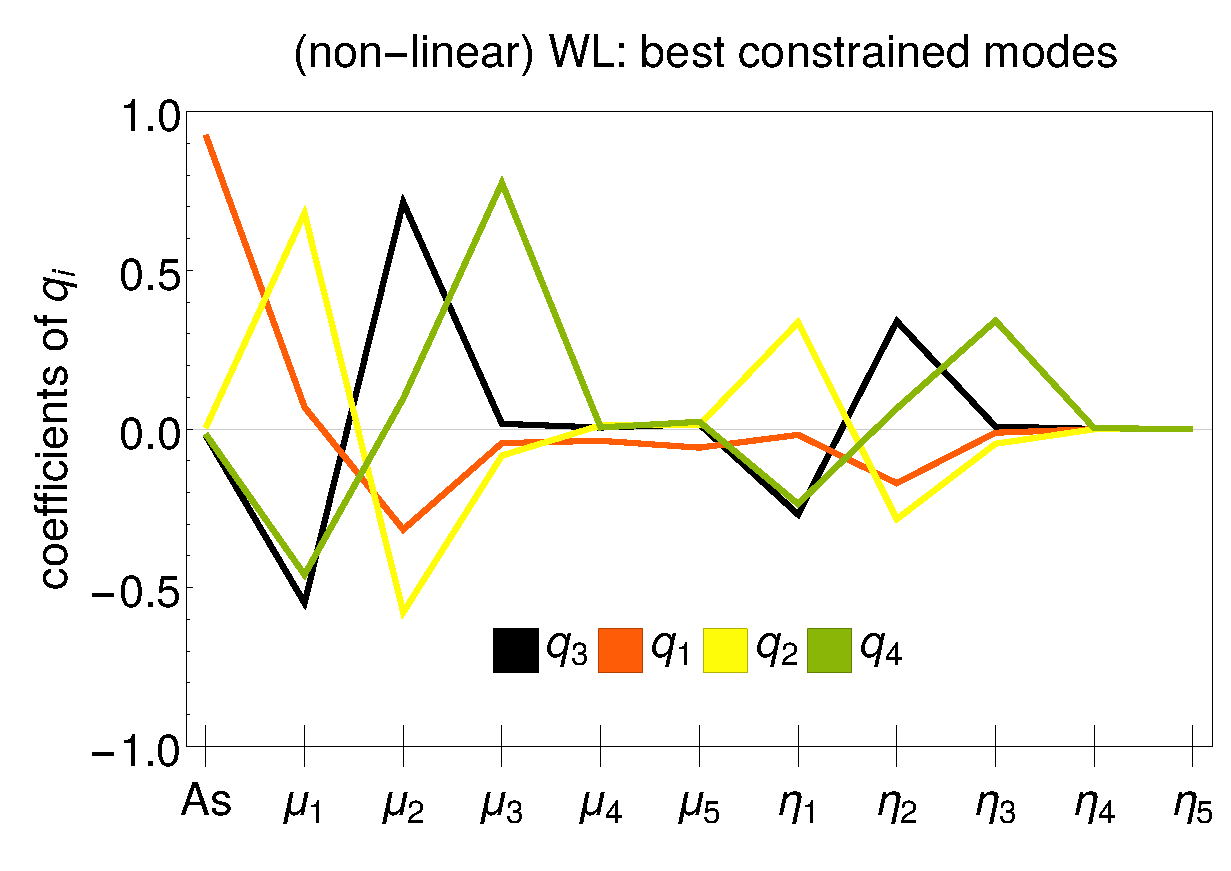
\includegraphics[width=0.47\linewidth]{Chapters/linear-nonlinear-MG-forecasts/figures/Decorrelations-WL/non-linear_WL--_best_constrained_modes-Errors_on_q_ZCA_SquareNorm--_fiducialMGBin3_Euclid_WL_nonlinearPk__Zhao_}
	\caption[Best constrained modes for Euclid GC applying ZCA.]{\label{fig:WLbestconst}
Best constrained modes for a Euclid Redbook WL survey, 
with $\mu$ and $\eta$ binned in redshift, after transforming into uncorrelated $q$ parameters via ZCA.
Each of the four best constrained parameters $q_i$, shown in the panels, is a linear combination of the primary parameters $p_i$. $q_i$ in the label are ordered from the best constrained to the least constrained.}
\end{figure}





\subsection{ZCA for Weak Lensing + Galaxy Clustering +  CMB \planck\ priors}

As mentioned earlier, Galaxy Clustering and Weak Lensing are particularly important, combined together, to constrain Modified Gravity parameters, as they probe two independent combinations of the gravitational potentials. We now show results for their combination, using for both the non-linear HS prescription, together with a \planck\ prior
 (which was obtained by performing an MCMC analysis on {\it Planck}+BSH background data, as specified in Section \ref{sub:Fisher-Planck}). Notice that we neglect here any
 information coming from the cross correlation of the two probes; we therefore assume that these two observables are independent of each other
and we simply add the GC and WL Fisher matrices to obtain our combined results; this appears to be a conservative (pessimistic) choice 
\cite{Lacasa2016}.
 In Table \ref{tab:errors-all-MGBin3}, we can see that the inclusion of the \planck\ prior improves considerably certain parameters, especially
 the less constrained ones by GC+WL, namely $\mu_{4,5}$ and $\eta_{4,5}$.
 In terms of correlations, we can observe in the left panel of Fig.\ \ref{fig:GC+WL+Planck-corr-Wmat}, that the structure of the correlation matrix resembles the one of the linear WL case (Fig.\ \ref{fig:WLcorr}), except that the block of standard $\lcdm$ parameters is much less correlated and that the anti-correlation among $\mu_i$ and $\eta_i$ is much stronger now.
On the other hand, applying the decorrelation procedure (\cref{sec:Decorrelation-of-covariance}), the weight matrix $W$ (right panel of Fig.\ \ref{fig:GC+WL+Planck-corr-Wmat}), resembles the $W$ matrix observed in the non-linear GC case, illustrated in Figure \ref{fig:Wmat-ZCA-GC}). Notice that now the variables $q_i$ depend quite strongly on only one of the $\mu_i$ for $i=\{1,2,3,4\}$, while the $q_i$ for $i=\{6,7,8,9,10\}$ depend on a balanced sum of $\mu_i$ and $\eta_i$ for $i=\{6,7,8,9,10\}$.

\begin{figure}[htbp]
	\centering
    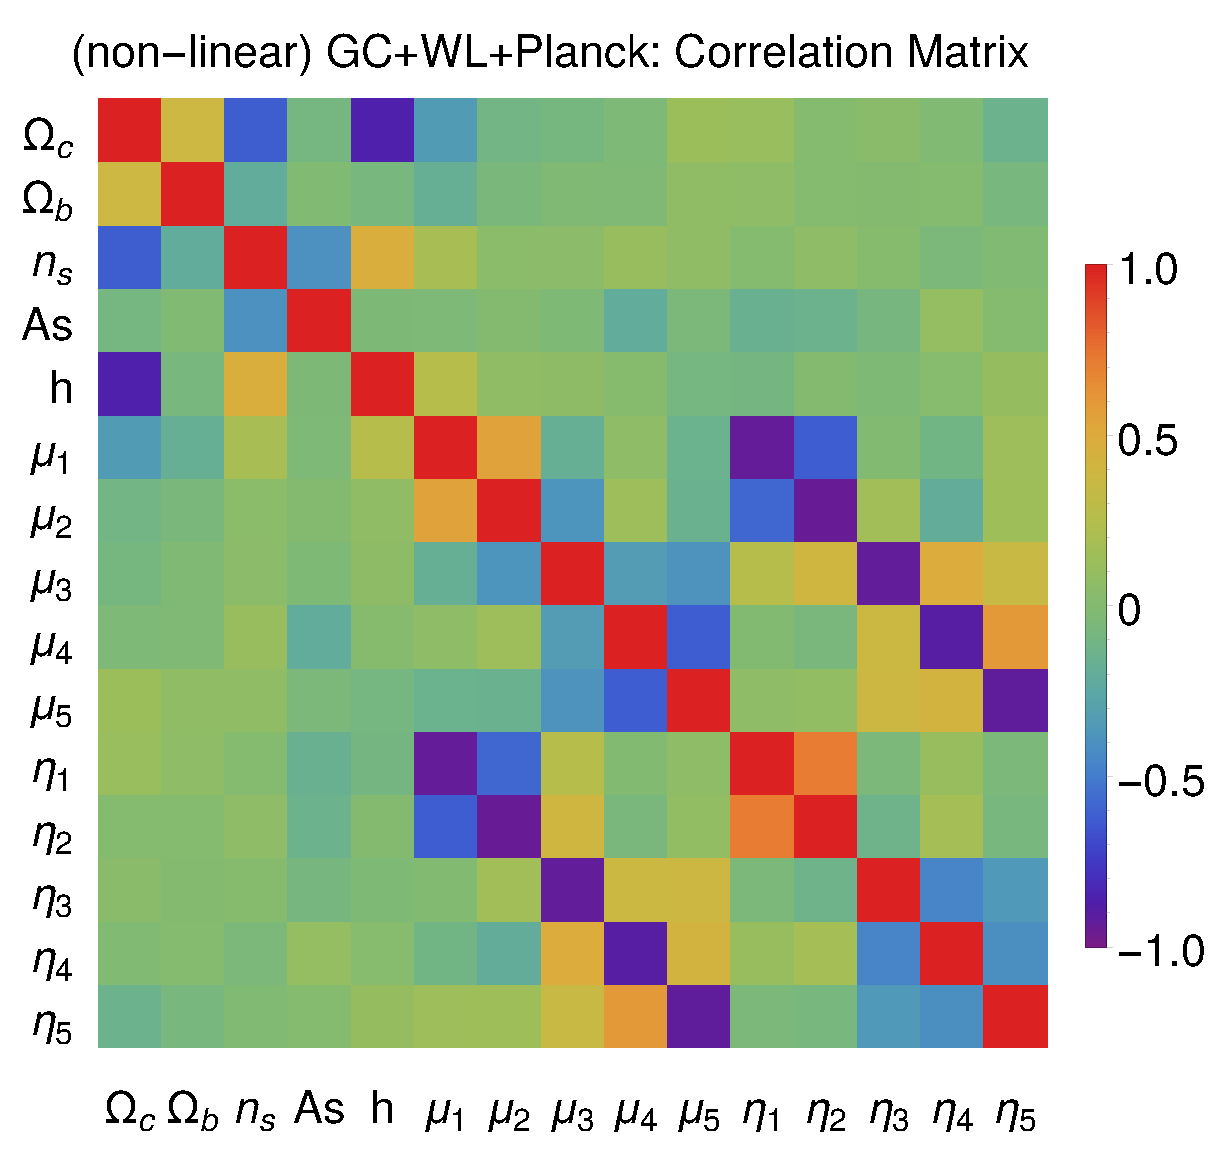
\includegraphics[width=0.47\linewidth]{Chapters/linear-nonlinear-MG-forecasts/figures/Decorrelations-GC+WL+Planck/correlation-full-fiducialMGBin3-Euclid-GC+WL+Planck-nonlinearPk__Zhao-}
    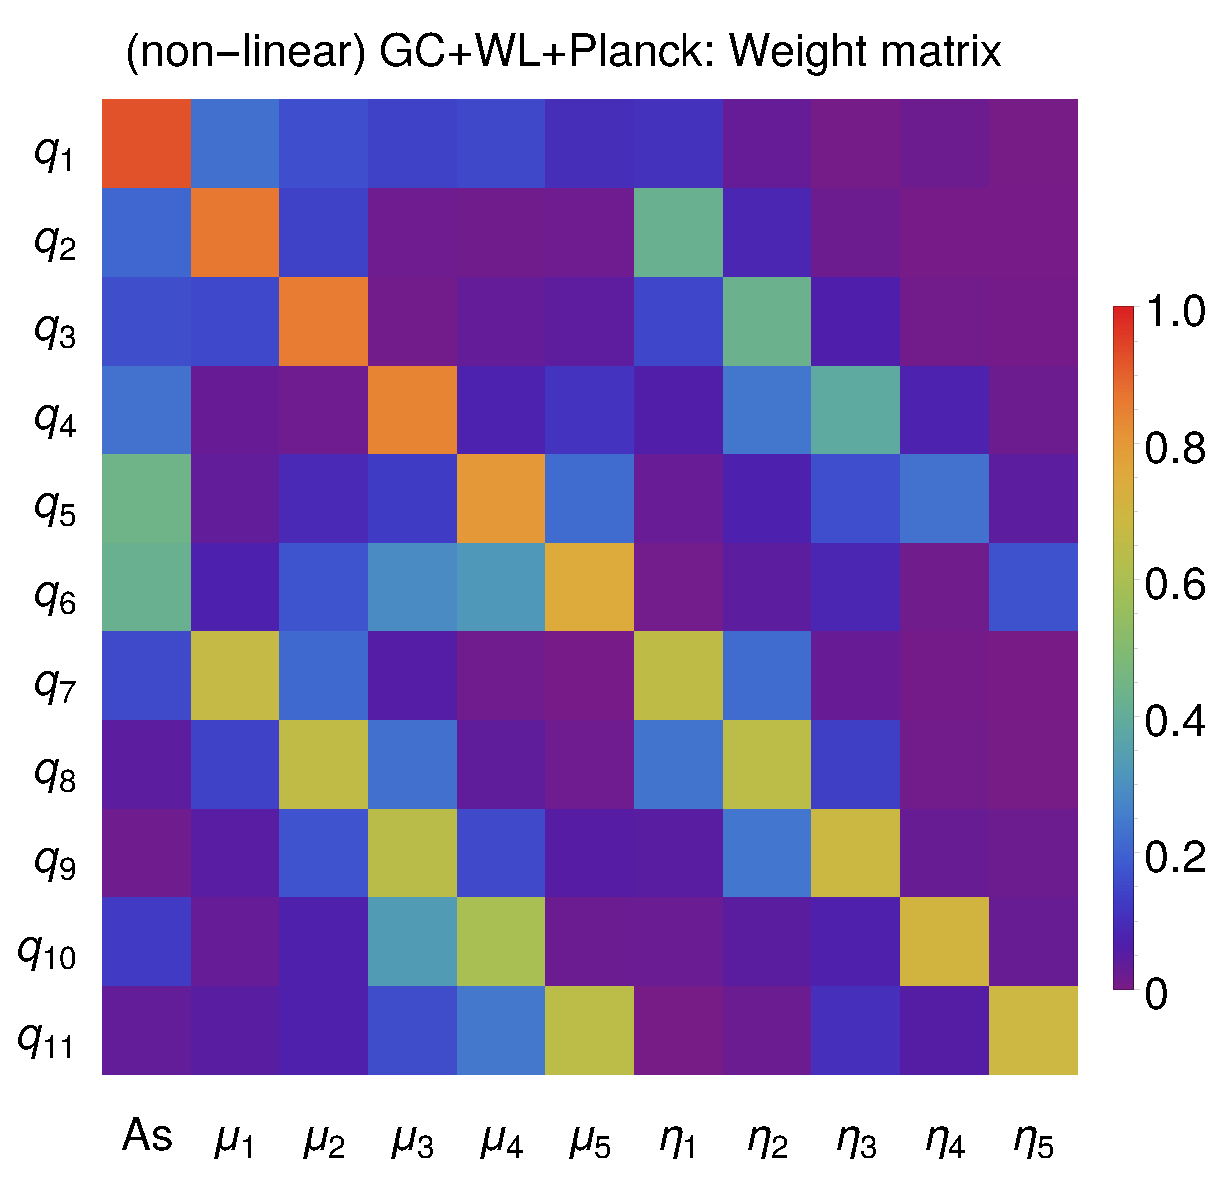
\includegraphics[width=0.47\linewidth]{Chapters/linear-nonlinear-MG-forecasts/figures/Decorrelations-GC+WL+Planck/Weight_Matrix_ZCA_SquareNorm--_fiducialMGBin3_Euclid_GC+WL+Planck_nonlinearPk__Zhao_}
	\caption[Correlation and Weight matrix for a Euclid GC+WL forecast.]{\label{fig:GC+WL+Planck-corr-Wmat}
Results for the combined forecasts of Euclid Redbook GC+WL using the non-linear HS prescription together with the addition 
of \planck\ CMB priors.
\textbf{Left panel:} correlation matrix obtained from the covariance matrix in the MG-binning case. 
Red (purple blue) colors represent strong positive (negative) correlations. 
The structure of this matrix is considerably diagonal, except for the strong anti-correlations of the pair $(\mu_i,\eta_i)$ 
for $i=\{1,2,3,4,5\}$, which resembles the correlations found for the WL case alone (see Figure \ref{fig:WLcorr}). 
However, the sub-block of standard cosmological parameters is now  much more diagonal 
and shows less correlations than in the GC (Fig.\ \ref{fig:GCcorr}) or WL cases.
The natural FoC (defined in \ref{eq:FoC}) in this case is $\approx 22$, showing that the variables are much less correlated 
than in the two previous cases.
\textbf{Right panel:} entries of the matrix $W$ for the ZCA decorrelation of the covariance matrix. 
This matrix shows for each new variable $q_i$ on the vertical axis, the coefficients of the 
linear combination of parameters $\mu_i$ and $\eta_i$ that give rise to that variable $q_i$. 
The red (blue) colors, indicate a large (small) contribution of the respective variable on the horizontal axis.}
\end{figure}


Finally, in this combined case the best constrained $q_i$ variables, are $q_1,\;q_2,\;q_3,\;$, $q_4$ approximately given by:
\begin{equation} \label{eq:bestCombined-GCWLnonlinPlanck}
\begin{aligned}
	q_1  &= +0.93\lAs\\            
	q_2  &= +0.84\mu_1 + 0.48\eta_1 \\ 
	q_3  &= +0.80\mu_2 - 0.26\eta_1 + 0.45 \eta_2\\
	q_4  &= +0.28\lAs + 0.79\mu_3 - 0.29 \eta_2 + 0.39 \eta_3 \,\,\, .
\end{aligned}
\end{equation}
These combinations of primary parameters are illustrated in the right panel of Figure \ref{fig:GC+WL+Planck-bestconst-errspq}.
The combination $q_2$ is similar to the combination $2\mu+\eta$ that was also identified in \cite{planck_collaboration_planck_2016} as being well-constrained. The best constrained modes $q_2$, $q_3$ and $q_4$ all contain terms of the form $a\mu_i + b\eta_i$ for $i=\{1,2,3\}$, with positive coefficients $a$ and $b$, where $a \approx 2b$.

All errors are shown in the left panel of Figure \ref{fig:GC+WL+Planck-bestconst-errspq}. Notice how in this case, the improvement on the errors of the $q_i$ variables is less than an order of magnitude, thus smaller than what found in GC and WL separately; this is due to combination of GC and WL which, together with the inclusion of the CMB prior, lead to smaller correlations among the parameters. 
When combining GC+WL in the non-linear HS case, the FoC (defined in \ref{eq:FoC}) is $\approx 31$, 
showing that there is not much gain in decorrelation, compared to GC or WL alone, where this quantity was approximately $32$.
However, combining GC+WL (non-linear HS) with \planck\ priors yields $\textrm{FoC} \approx 22$, showing that correlations among
parameters are drastically reduced.
The fact that the curve of 1$\sigma$ errors for the $q_i$ (orange line, marked with circles) 
follows the same pattern as the curve for the $p_i$ errors (green dashed line, marled with circles), 
is due to the fact that we have used a ZCA decomposition and therefore the $q_i$ are as close as possible to the $p_i$.
%The complete matrix of coefficients $W$ can be found in Table \ref{tab:Wcoeff-nlHS-WL+GC+Planck} in appendix \ref{sec:Wmatrices}.


\begin{figure}[htbp]
	\centering
	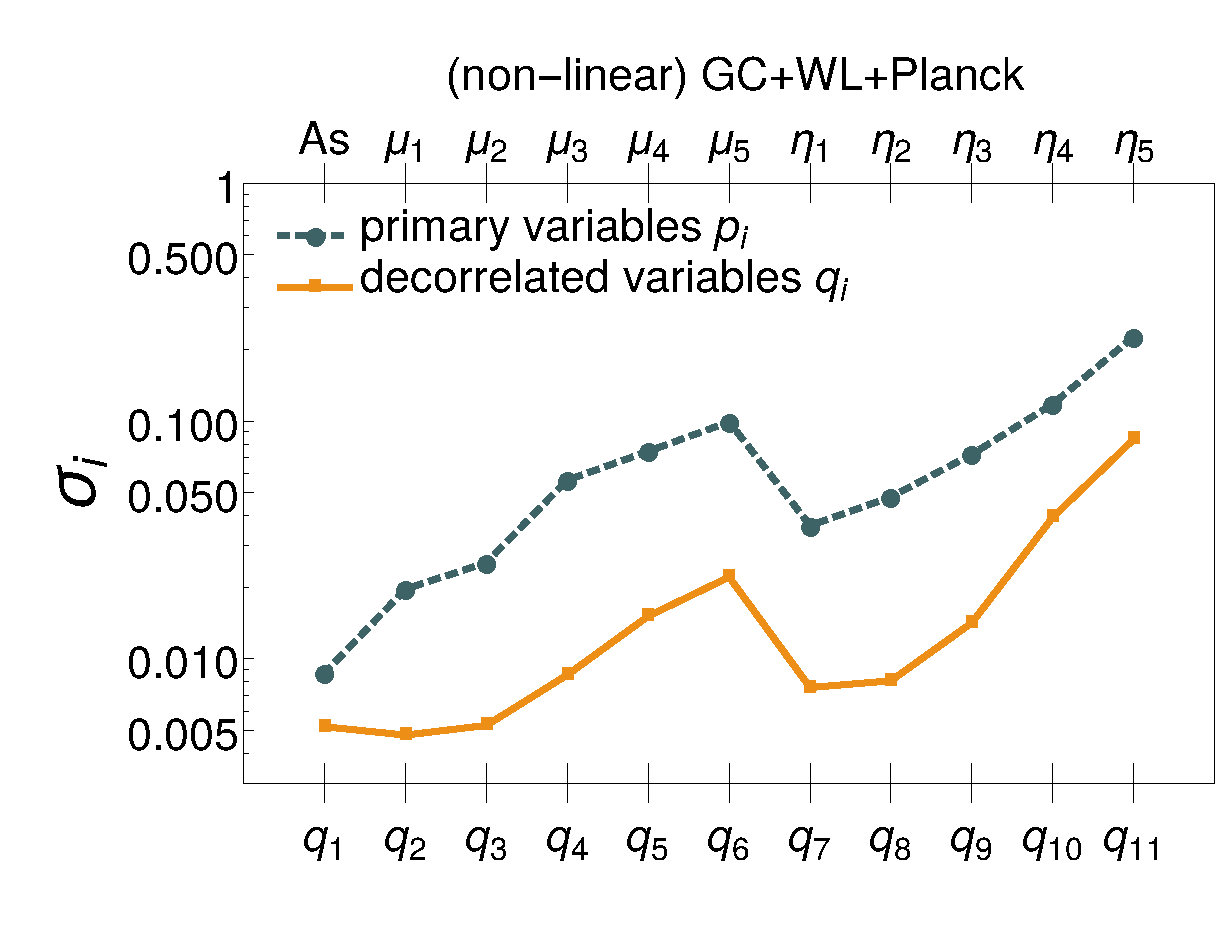
\includegraphics[width=0.49\linewidth]{Chapters/linear-nonlinear-MG-forecasts/figures/Decorrelations-GC+WL+Planck/Errors_at_par_index_i--_ZCA_SquareNorm--fiducialMGBin3_Euclid_GC+WL+Planck_nonlinearPk__Zhao_}
	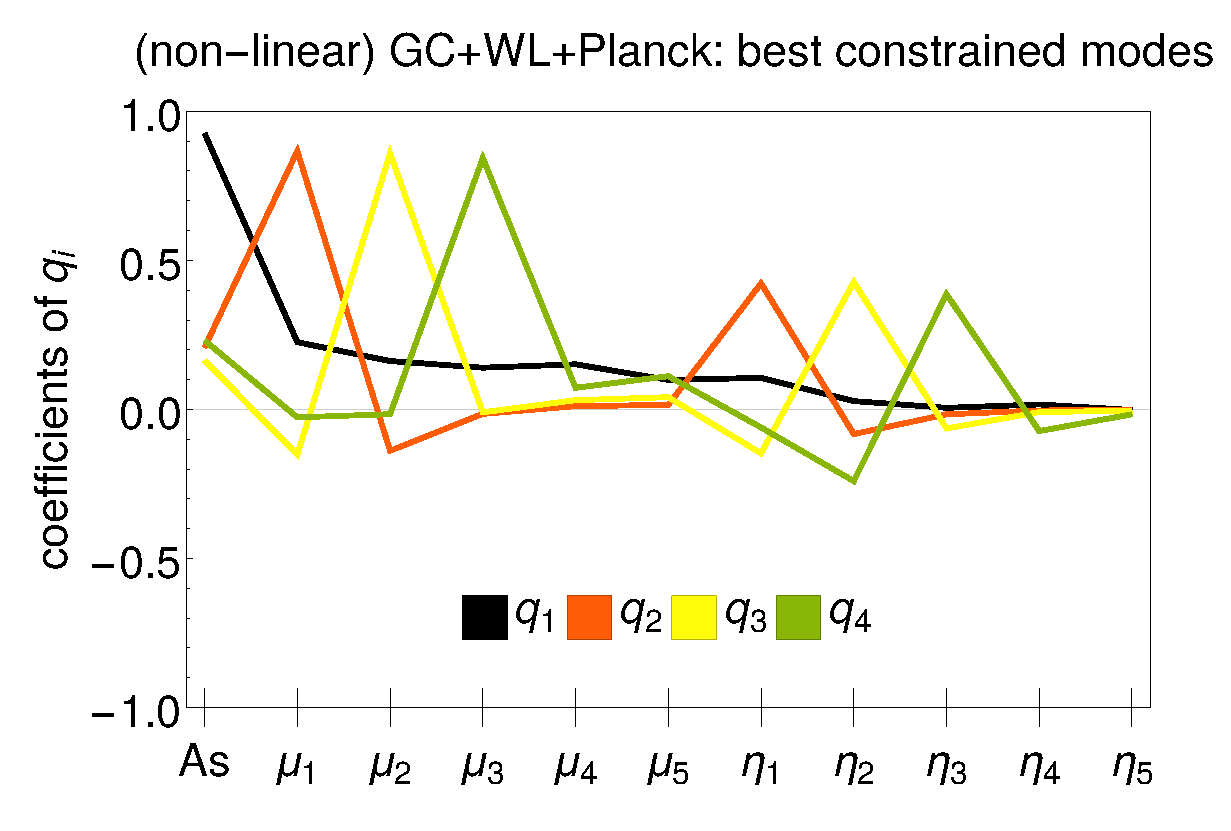
\includegraphics[width=0.49\linewidth]{Chapters/linear-nonlinear-MG-forecasts/figures/Decorrelations-GC+WL+Planck/non-linear_GC+WL+Planck--_best_constrained_modes-Errors_on_q_ZCA_SquareNorm--_fiducialMGBin3_Euclid_GC+WL+Planck_nonlinearPk__Zhao_}
	\caption[1$\sigma$ forecasted errors and best constrained modes for a Euclid GC+WL forecast.]{\label{fig:GC+WL+Planck-bestconst-errspq}
		\textbf{Left:} the 1$\sigma$ fully marginalized errors on the primary parameters $p_i$ (green dashed
		lines), and the 1$\sigma$ errors on the decorrelated derived
		parameters $q_i$ (yellow solid lines). As opposed to the GC or WL cases (figs.\ref{fig:GCbinerrs},\ref{fig:WLbinerrs}), here the decorrelated errors are much more similar to the standard errors.
		This is due to the fact that in the GC+WL+{\it Planck} combination, the cosmological parameters are not so strongly correlated.
		\textbf{Right:} best constrained modes for a Euclid Redbook GC+WL case using the non-linear HS prescription and adding a CMB \planck\ prior.
		Each panel shows the four best constrained parameters $q_i$. Each of them is a linear combination of the primary parameters $p_i$. 
		The best constrained modes are sums $a\mu_i + b\eta_i$ for $i=\{1,2,3\}$ and positive values $a$ and $b$.}
\end{figure}

\begin{sidewaystable}%[htbp]
\centering{}%
\small
\begin{tabular}{|l|c|c|c|c|c|c|c|c|c|c|c||c|}
\hline 
\Tstrut \textbf{Euclid} (Redbook)  & $\ell \mathcal{A}_{s}$  & $\mu_{1}$  & $\mu_{2}$  & $\mu_{3}$  & $\mu_{4}$  & $\mu_{5}$  & $\eta_{1}$  
& $\eta_{2}$  & $\eta_{3}$  & $\eta_{4}$ & $\eta_{5}$ & MG FoM
\tabularnewline
\hline 
\Tstrut Fiducial  & 3.057  & 1.108  & 1.027  & 0.973  & 0.952  & 0.962  & 1.135  & 1.160  & 1.219  & 1.226 & 1.164 &  relative\tabularnewline
\hline 
\Tstrut \textbf{GC (lin)}  \Tstrut & 160\% & 119\% & 159\% & 183\% & 450\% & 1470\% & 509\% & 570\% & 586\% & 728\% & 3390\%  & 0 \tabularnewline
\Tstrut \textbf{GC (nl-HS)} \Tstrut & 0.8\% & 7.0\% & 6.7\% & 10.9\% & 27.4\% & 41.1\% & 20\% & 24.3\% & 19.9\% & 38.2\% & 930\% & 19  \tabularnewline
\hline
\hline
\Tstrut \textbf{WL (lin)}  & 640\% & 165\% & 2210\% & 4150\% & 13100\% & 22500\% & 2840\% & 3140\% & 8020\% & 29300\% & 39000\%  
& -27\tabularnewline
\Tstrut \textbf{WL (nl-HS)}  & 7.3\% & 188\% & 255\% & 419\% & 222\% & 206\% & 330\% & 488\% & 775\% & 8300\% & 9380\% 
& -10  \tabularnewline
\hline
\hline
\Tstrut \textbf{GC+WL (lin)} & 11.3\% & 5.8\% & 10\% & 19.2\% & 282\% & 469\% & 7.9\% & 9.6\% & 16.1\% & 276\% & 2520\%
& 12  \tabularnewline
\Tstrut \textbf{GC+WL+{\it Planck} (lin)} & 1.1\% & 3.4\% & 4.8\% & 7.8\% & 9.3\% & 13.1\% & 6.2\% & 7.7\% & 9.1\% & 12.7\% & 23.6\%
& 27 \tabularnewline
\hline
\hline
\Tstrut \textbf{GC+WL (nl-HS)} & 0.8\% & 2.2\% & 3.3\% & 8.2\% & 24.8\% & 34.1\% & 3.6\% & 5.1\% & 8.1\% & 25.4\% & 812\%
& 24 \tabularnewline
\Tstrut \textbf{GC+WL+{\it Planck}} &  &   &  &   &  &   &   &  &   &  & & 
\tabularnewline \textbf{(nl-HS)}  
& 0.3\% & 1.8\% & 2.5\% & 5.8\% & 7.8\% & 10.3\% & 3.2\% & 4.1\% & 5.9\% & 9.6\% & 19.5\% 
& 33 \tabularnewline
\Tstrut \textbf{GC+WL+{\it Planck}} &  &   &  &   &  &   &   &  &   &  & & 
\tabularnewline \textbf{(nl-Halofit)}  
& 0.4\% & 2.0\% & 2.4\% & 5.1\% & 7.4\% & 10.2\% & 3.5\% & 4.1\% & 5.8\% & 9.2\% & 18.9\% 
& 33 \tabularnewline
\hline
\end{tabular}
\small
\protect\caption[1$\sigma$ marginalized errors for a Euclid GC and WL survey in a redshift binned scenario of MG.]{\label{tab:errors-all-MGBin3}
1$\sigma$
fully marginalized errors (as a percentage of the corresponding fiducial) on cosmological parameters for Euclid (Redbook) Galaxy Clustering and Weak Lensing surveys, alone and combining the two probes. We compare forecasts using linear spectra (lin) and forecasts using the nonlinear HS prescription (nl-HS). In Galaxy Clustering, the cutoff is set to $k_{\rm max}=0.15$ h/Mpc in the linear case and $k_{\rm max}=0.5$ h/Mpc in the non-linear case.
For WL, the maximum cutoff in the linear case is at $\ell_{\rm max} = 1000$, 
while in the nl-HS case it is $\ell_{\rm max} = 5000$.
At the bottom, we add on top a \planck\ prior (see section \ref{sub:Fisher-Planck}).
For comparison, we also show in the last row the combined GC+WL+{\it Planck}, using just Halofit power spectra. 
The last column indicates the relative Figure of Merit ($\text{FoM}_{a,b}$) of the MG parameters in nits (`natural units', i.e.\ using the natural logarithm), with respect to our reference GC linear case, see (\ref{eq:FoM}) and surrounding text. A larger FoM indicates a more constraining probe. We notice a considerable improvement, in both GC and WL, when non-linearities are included.
The combination GC+WL in the linear case 
constrains the MG parameters in the first two bins (z < 1.0 ) to less than 10$\%$ and including \planck\ priors allows to access higher redshifts with the same accuracy. A significant improvement in the constraints is obtained when adding the non-linear regime, in agreement with the observed reduction in correlation seen in Figs.\ \ref{fig:GCcorr} and \ref{fig:WLcorr}. This is especially well exemplified by the error on $\ell \mathcal{A}_s \equiv \ln(10^{10} A_{s})$, which reduces from 160\%  to 0.82\%, from the linear to the non-linear forecast in the GC case
and from 640\%  to 7.3\% in the WL case. 
Finally, we note that since we are showing errors on $\mu$ and $\eta$, WL seems to be unfairly poor at constraining parameters. However, when converting this errors into errors on $\Sigma$, which is directly measured by WL, the constrains on $\Sigma_{1,2,3}$ are slightly better, of the order of 40\% for WL(nl-HS) as can be guess from the degeneracy directions shown in Fig.\ \ref{fig:DE+Planck-ellipses-mu-sig-eta}. The FoM itself is nearly unaffected by the choice of $\{\mu,\eta\}$ vs $\{\mu,\Sigma\}$ as it is rotationally invariant.
}
\end{sidewaystable}
\normalsize

%\section{Weight matrices coefficients}
%\label{sec:Wmatrices}
%
%Here we explicitly show the coefficient of the $W$ matrices illustrated in Figures
%\ref{fig:Wmat-ZCA-GC}, \ref{fig:Wmat-ZCA-WL}
%and \ref{fig:GC+WL+Planck-corr-Wmat}.
%Tables \ref{tab:Wcoeff-lin-GC} and \ref{tab:Wcoeff-nlHS-GC} contain the coefficient matrices obtained for 
%Galaxy Clustering in the linear and non-linear HS prescription cases respectively, while 
%Tables \ref{tab:Wcoeff-lin-WL} and \ref{tab:Wcoeff-nlHS-WL} contain the coefficients obtained for WL. 
%Finally, Table \ref{tab:Wcoeff-nlHS-WL+GC+Planck} reports the coefficients for the combination of GC, 
%WL and \planck\ priors, in the non-linear HS case.

%\begin{table}[H]
%	\[
%	q_i = 
%	\footnotesize
%	\left(
%	\begin{array}{rrrrrrrrrrr}
%	\color{red} 0.899 & 0.003 & -0.020 & 0.109 & \color{red} 0.315 & 0.250 & 0.097 & 0.021 & -0.083 & -0.022 & -0.007 \\
%	0.001 & \color{red} 0.695 & \color{red} -0.304 & -0.089 & -0.084 & -0.026 & \color{red} 0.519 & \color{red} -0.362 & -0.082 & -0.033 & 0.001 \\
%	-0.003 & -0.186 & \color{red} 0.745 & -0.211 & -0.090 & -0.027 & \color{red} -0.285 & \color{red} 0.491 & -0.181 & -0.036 & 0.001 \\
%	0.022 & -0.065 & \color{red} -0.252 & \color{red} 0.737 & -0.174 & -0.019 & -0.075 & \color{red} -0.320 & \color{red} 0.486 & -0.116 & 0.001 \\
%	0.148 & -0.142 & -0.250 & \color{red} -0.405 & \color{red} 0.666 & 0.070 & -0.094 & -0.102 & \color{red} -0.268 & \color{red} 0.439 & -0.002 \\
%	\color{red} 0.654 & -0.246 & \color{red} -0.420 & -0.240 & \color{red} 0.388 & \color{red} 0.290 & 0.098 & 0.086 & -0.159 & 0.003 & -0.008 \\
%	0.026 & \color{red} 0.494 & \color{red} -0.444 & -0.098 & -0.053 & 0.010 & \color{red} 0.621 & \color{red} -0.375 & -0.129 & -0.055 & -0.000 \\
%	0.004 & \color{red} -0.265 & \color{red} 0.588 & \color{red} -0.320 & -0.044 & 0.007 & \color{red} -0.288 & \color{red} 0.578 & -0.248 & -0.045 & -0.000 \\
%	-0.023 & -0.082 & \color{red} -0.295 & \color{red} 0.664 & -0.158 & -0.017 & -0.135 & \color{red} -0.338 & \color{red} 0.545 & -0.102 & 0.001 \\
%	-0.015 & -0.082 & -0.147 & \color{red} -0.399 & \color{red} 0.651 & 0.001 & -0.146 & -0.155 & \color{red} -0.257 & \color{red} 0.525 & -0.000 \\
%	\color{red} -0.519 & \color{red} 0.308 & \color{red} 0.510 & \color{red} 0.346 & \color{red} -0.348 & -0.239 & -0.061 & -0.070 & 0.181 & -0.004 & 0.193 \\
%	\end{array}
%	\right)
%	\cdot 
%    \footnotesize	
%	\begin{pmatrix} \ln(10^{10}A_s) \\ \mu_{1}  \\ \mu_{2}   \\ \mu_{3}   \\ \mu_{4}   \\ \mu_{5}  
%	\\ \eta_{1}   \\ \eta_{2}  \\ \eta_{3}   \\\eta_{4}  \\ \eta_{5}
%	\end{pmatrix}
%	\]
%	\caption{\label{tab:Wcoeff-lin-GC}
%		\normalfont Coefficients of the Matrix $W$ for the Euclid Redbook GC forecasted covariance matrix, using linear power spectra.
%		The entries marked with red are those whose absolute values are larger than $0.25$.}
%\end{table}
%\begin{table}[H]
%	\[
%	q_i = 
%	\footnotesize
%	\left(
%	\begin{array}{rrrrrrrrrrr}
%	\color{red} 0.986 & -0.064 & -0.112 & -0.093 & -0.037 & -0.038 & -0.002 & 0.005 & -0.002 & 0.005 & 0.002 \\
%	-0.021 & \color{red} 0.677 & \color{red} -0.349 & -0.091 & -0.042 & -0.008 & \color{red} 0.516 & \color{red} -0.367 & -0.086 & -0.021 & 0.001 \\
%	-0.025 & -0.233 & \color{red} 0.731 & -0.194 & -0.051 & -0.011 & \color{red} -0.317 & \color{red} 0.492 & -0.166 & -0.021 & 0.001 \\
%	-0.030 & -0.088 & \color{red} -0.281 & \color{red} 0.755 & -0.061 & 0.036 & -0.073 & \color{red} -0.331 & \color{red} 0.465 & -0.086 & -0.001 \\
%	-0.032 & -0.108 & -0.197 & -0.161 & \color{red} 0.820 & 0.238 & -0.023 & -0.092 & -0.240 & \color{red} 0.357 & -0.007 \\
%	-0.086 & -0.058 & -0.110 & \color{red} 0.252 & \color{red} 0.637 & \color{red} 0.659 & 0.224 & -0.001 & -0.143 & -0.046 & -0.018 \\
%	-0.001 & \color{red} 0.492 & \color{red} -0.452 & -0.071 & -0.008 & 0.031 & \color{red} 0.617 & \color{red} -0.391 & -0.113 & -0.038 & -0.001 \\
%	0.001 & \color{red} -0.296 & \color{red} 0.593 & \color{red} -0.275 & -0.029 & -0.000 & \color{red} -0.331 & \color{red} 0.575 & -0.209 & -0.031 & -0.000 \\
%	-0.001 & -0.115 & \color{red} -0.329 & \color{red} 0.635 & -0.124 & -0.028 & -0.157 & \color{red} -0.344 & \color{red} 0.558 & -0.065 & 0.001 \\
%	0.008 & -0.092 & -0.136 & \color{red} -0.390 & \color{red} 0.614 & -0.030 & -0.176 & -0.167 & -0.216 & \color{red} 0.581 & 0.001 \\
%	0.140 & 0.126 & 0.180 & -0.194 & \color{red} -0.645 & \color{red} -0.608 & -0.218 & -0.029 & 0.137 & 0.049 & 0.199 \\
%	\end{array}
%	\right)
%		\cdot 
%	\footnotesize	
%    \begin{pmatrix} \ln(10^{10}A_s) \\ \mu_{1}  \\ \mu_{2}   \\ \mu_{3}   \\ \mu_{4}   \\ \mu_{5}  
%	\\ \eta_{1}   \\ \eta_{2}  \\ \eta_{3}   \\\eta_{4}  \\ \eta_{5}
%	\end{pmatrix}
%	\]
%	\caption{\label{tab:Wcoeff-nlHS-GC}
%		\normalfont Coefficients of the Matrix $W$ for the Euclid Redbook GC forecasted covariance matrix, using the non-linear HS prescription.
%		The entries marked with red are those whose absolute values are larger than $0.25$.}
%\end{table}
%\begin{table}[H]
%	\[
%	q_i = 
%	\footnotesize
%	\left(
%	\begin{array}{rrrrrrrrrrr}
%	\color{red} 0.760 & -0.005 & \color{red} 0.475 & 0.131 & 0.005 & 0.034 & 0.247 & \color{red} 0.329 & 0.095 & 0.004 & -0.000 \\
%	-0.000 & \color{red} 0.673 & \color{red} -0.592 & -0.055 & 0.013 & 0.008 & \color{red} 0.328 & \color{red} -0.290 & -0.034 & -0.001 & -0.000 \\
%	0.033 & \color{red} -0.594 & \color{red} 0.674 & 0.013 & -0.003 & -0.000 & \color{red} -0.302 & \color{red} 0.318 & 0.010 & 0.000 & 0.000 \\
%	0.075 & \color{red} -0.457 & 0.112 & \color{red} 0.754 & 0.002 & 0.004 & \color{red} -0.310 & 0.039 & \color{red} 0.326 & 0.001 & 0.000 \\
%	0.022 & \color{red} 0.892 & -0.187 & 0.017 & 0.102 & 0.064 & \color{red} 0.326 & -0.208 & -0.064 & -0.000 & 0.000 \\
%	\color{red} 0.251 & \color{red} 0.859 & -0.030 & 0.048 & 0.098 & 0.090 & \color{red} 0.414 & -0.078 & -0.029 & 0.004 & 0.009 \\
%	0.034 & \color{red} 0.654 & \color{red} -0.600 & -0.074 & 0.009 & 0.008 & \color{red} 0.356 & \color{red} -0.280 & -0.037 & -0.000 & 0.000 \\
%	0.047 & \color{red} -0.606 & \color{red} 0.662 & 0.010 & -0.006 & -0.002 & \color{red} -0.293 & \color{red} 0.324 & 0.013 & 0.001 & 0.001 \\
%	0.108 & \color{red} -0.576 & 0.167 & \color{red} 0.655 & -0.015 & -0.005 & \color{red} -0.311 & 0.105 & \color{red} 0.304 & 0.003 & 0.002 \\
%	\color{red} 0.256 & \color{red} -0.718 & \color{red} 0.380 & 0.136 & -0.003 & 0.032 & -0.010 & \color{red} 0.448 & 0.197 & 0.111 & 0.061 \\
%	-0.029 & \color{red} -0.734 & \color{red} 0.253 & 0.068 & 0.000 & 0.166 & 0.084 & \color{red} 0.506 & 0.218 & 0.122 & 0.197 \\
%	\end{array}
%	\right)
%	\cdot 
%	\footnotesize
%	\begin{pmatrix} \ln(10^{10}A_s) \\ \mu_{1}  \\ \mu_{2}   \\ \mu_{3}   \\ \mu_{4}   \\ \mu_{5}  
%	\\ \eta_{1}   \\ \eta_{2}  \\ \eta_{3}   \\\eta_{4}  \\ \eta_{5}
%	\end{pmatrix}
%	\]
%	\caption{\label{tab:Wcoeff-lin-WL}
%		\normalfont Coefficients of the Matrix $W$ for the Euclid Redbook WL forecasted covariance matrix, using linear power spectra.
%		The entries marked with red are those whose absolute values are larger than $0.25$.}
%\end{table}
%\begin{table}[H]
%	\[
%	q_i = \left(
%	\footnotesize
%	\begin{array}{rrrrrrrrrrr}
%	\color{red} 0.926 & -0.004 & \color{red} -0.323 & -0.039 & -0.040 & -0.066 & -0.043 & -0.168 & -0.004 & -0.000 & 0.001 \\
%	-0.000 & \color{red} 0.669 & \color{red} -0.595 & -0.051 & 0.012 & 0.013 & \color{red} 0.332 & \color{red} -0.291 & -0.031 & -0.001 & -0.000 \\
%	-0.021 & \color{red} -0.552 & \color{red} 0.711 & 0.029 & 0.005 & 0.016 & \color{red} -0.270 & \color{red} 0.339 & 0.014 & 0.001 & 0.000 \\
%	-0.025 & \color{red} -0.460 & \color{red} 0.288 & \color{red} 0.725 & 0.016 & 0.040 & -0.238 & 0.150 & \color{red} 0.312 & 0.002 & 0.000 \\
%	-0.159 & \color{red} 0.657 & \color{red} 0.289 & 0.102 & \color{red} 0.476 & 0.156 & \color{red} 0.418 & 0.155 & -0.007 & 0.006 & 0.001 \\
%	-0.168 & \color{red} 0.455 & \color{red} 0.622 & 0.158 & 0.100 & \color{red} 0.486 & 0.223 & 0.236 & -0.016 & -0.001 & -0.002 \\
%	-0.006 & \color{red} 0.667 & \color{red} -0.585 & -0.053 & 0.015 & 0.012 & \color{red} 0.366 & \color{red} -0.274 & -0.026 & 0.000 & -0.000 \\
%	-0.023 & \color{red} -0.560 & \color{red} 0.704 & 0.032 & 0.005 & 0.013 & \color{red} -0.263 & \color{red} 0.345 & 0.017 & 0.001 & 0.000 \\
%	-0.005 & \color{red} -0.576 & \color{red} 0.277 & \color{red} 0.636 & -0.002 & -0.008 & -0.238 & 0.165 & \color{red} 0.319 & 0.004 & 0.001 \\
%	-0.026 & \color{red} -0.506 & \color{red} 0.670 & 0.239 & 0.110 & -0.037 & 0.114 & \color{red} 0.359 & 0.209 & 0.169 & 0.096 \\
%	0.180 & \color{red} -0.799 & 0.053 & 0.033 & 0.069 & -0.140 & -0.055 & 0.044 & 0.134 & \color{red} 0.271 & \color{red} 0.452 \\
%	\end{array}
%	\right)
%	\cdot
%	\footnotesize 
%	\begin{pmatrix} \ln(10^{10}A_s) \\ \mu_{1}  \\ \mu_{2}   \\ \mu_{3}   \\ \mu_{4}   \\ \mu_{5}  
%	\\ \eta_{1}   \\ \eta_{2}  \\ \eta_{3}   \\\eta_{4}  \\ \eta_{5}
%	\end{pmatrix}
%	\]
%	\caption{\label{tab:Wcoeff-nlHS-WL}
%		\normalfont Coefficients of the Matrix $W$ for the Euclid Redbook WL forecasted covariance matrix, using the non-linear HS prescription.
%		The entries marked with red are those whose absolute values are larger than $0.25$.}
%\end{table}
%\begin{table}[H]
%	\[
%	q_i = \left(
%	\footnotesize
%\begin{array}{rrrrrrrrrrr}
%\color{red} 0.932 & 0.033 & 0.149 & 0.220 & 0.202 & 0.138 & -0.005 & -0.026 & -0.001 & 0.010 & -0.003 \\
%0.029 & \color{red} 0.839 & -0.214 & -0.085 & -0.035 & -0.021 & \color{red} 0.476 & -0.119 & -0.021 & 0.002 & -0.000 \\
%0.138 & -0.222 & \color{red} 0.800 & -0.083 & 0.016 & 0.028 & \color{red} -0.256 & \color{red} 0.452 & -0.118 & -0.011 & -0.002 \\
%\color{red} 0.284 & -0.123 & -0.115 & \color{red} 0.791 & 0.076 & 0.108 & -0.106 & \color{red} -0.286 & \color{red} 0.387 & -0.067 & -0.010 \\
%\color{red} 0.506 & -0.097 & 0.043 & 0.148 & \color{red} 0.753 & 0.248 & -0.059 & -0.089 & -0.144 & 0.222 & -0.032 \\
%\color{red} 0.545 & -0.092 & 0.120 & \color{red} 0.331 & \color{red} 0.390 & \color{red} 0.626 & -0.027 & -0.088 & -0.089 & -0.009 & 0.104 \\
%-0.006 & \color{red} 0.621 & \color{red} -0.322 & -0.096 & -0.028 & -0.008 & \color{red} 0.656 & \color{red} -0.261 & -0.048 & -0.009 & -0.001 \\
%-0.032 & -0.166 & \color{red} 0.605 & \color{red} -0.276 & -0.044 & -0.028 & \color{red} -0.277 & \color{red} 0.654 & -0.148 & -0.006 & 0.000 \\
%-0.003 & -0.049 & \color{red} -0.270 & \color{red} 0.634 & -0.122 & -0.048 & -0.088 & \color{red} -0.252 & \color{red} 0.659 & -0.023 & 0.010 \\
%0.067 & 0.015 & -0.082 & \color{red} -0.358 & \color{red} 0.614 & -0.017 & -0.055 & -0.034 & -0.074 & \color{red} 0.688 & 0.027 \\
%-0.072 & -0.002 & -0.060 & -0.179 & \color{red} -0.286 & \color{red} 0.591 & -0.027 & 0.008 & 0.108 & 0.088 & \color{red} 0.713 \\
%\end{array}
%	\right)
%	\cdot 
%	\footnotesize
%	\begin{pmatrix} \ln(10^{10}A_s) \\ \mu_{1}  \\ \mu_{2}   \\ \mu_{3}   \\ \mu_{4}   \\ \mu_{5}  
%	\\ \eta_{1}   \\ \eta_{2}  \\ \eta_{3}   \\\eta_{4}  \\ \eta_{5}
%	\end{pmatrix}
%	\]
%	\caption{\label{tab:Wcoeff-nlHS-WL+GC+Planck}
%		\normalfont Coefficients of the Matrix $W$ for the Euclid Redbook GC+WL case using the non-linear HS prescription and adding a CMB \planck\ prior.
%	     The entries marked with red are those whose absolute values are larger than $0.25$.}
%\end{table}



\section{Other Decorrelation Methods}\label{sec:appdec}

In \cref{sec:Decorrelation-of-covariance} we have worked with a special decorrelation method, ZCA (Zero-phase component analysis, first 
introduced by \cite{Bell19973327} in the context of image processing), which
allows us to find a new vector of decorrelated variables $q$ that is as similar as possible to the original
vector of variables $p$.
Other decorrelation methods do not share this property,
so in this section we want to illustrate their difference 
with respect to ZCA.
In the next subsections we show for the Principal Component Analysis and Cholesky decomposition methods, 
a subset of our previous results, namely the Galaxy Clustering non-linear case, 
using the HS prescription for a Euclid survey with Redbook specifications.

\subsubsection{Principal Component Analysis }

Principal Component Analysis (PCA) \cite{Friedman-PCA} is a well known method, which rotates
the vector of variables $p$ into a new basis, using the eigenmatrix of the 
covariance matrix $C$. At the same time, it is the method that maximizes the compression of all components
of $p$ into the components of $q$ using as measure the cross-covariance
between $q$ and $p$ (see \cite{kessy_optimal_2015} for more details and references).
This method is useful for dimensional reduction or data compression, 
since the information is stored in as few components as possible.
This is achieved by using the $W$ matrix

\begin{equation}
W=\Lambda^{-1/2}U^{T}
\end{equation}
where $\Lambda$ and $U$ represent the eigensystem of $C$ (defined in Eqn.\ \ref{eq:eigensystemofC}).

Then, it follows that the transformed covariance matrix $\tilde{C}$ is whitened:
\begin{align}
\tilde{C} & =\Lambda^{-1/2}U^{T}C\Lambda^{-1/2}U^{T}\\
& =\Lambda^{-1/2}U^{T}U\Lambda U^{T}\Lambda^{-1/2}U^{T}\\
& =\mathbbm{1}
\end{align}
As done previously, we renormalize $W$ in such a way that the sum of the square of the elements of each row sum up to
unity.
In Figure \ref{fig:PCA-GCnlhs} we show in the left panel the weight matrix $W$ and in the right panel the 1$\sigma$ errors for the original
and decorrelated variables. We see that the most constrained $q$ variables are the last components $q_8$-$q_{11}$, where most
of the information has been compressed into. These 4 variables are complicated linear combinations of $A_s$, $\mu_{1,2,3}$ 
and $\eta_{1,2,3}$. This is the same we found for ZCA (cf.\ Fig.\ \ref{fig:GCbestconst} and Eqns.\ (\ref{fig:GCbestconst})). However, the interpretation
in terms of the old variables $p$ is not so simple anymore. We can see from the weight matrix and the 1$\sigma$
errors, that the most unconstrained parameter is $q_1$, which is basically equivalent to $\eta_5$. This means that this parameter can be
eliminated from the analysis if one wants to do dimensional reduction.
\begin{figure}[htbp]
	\centering
	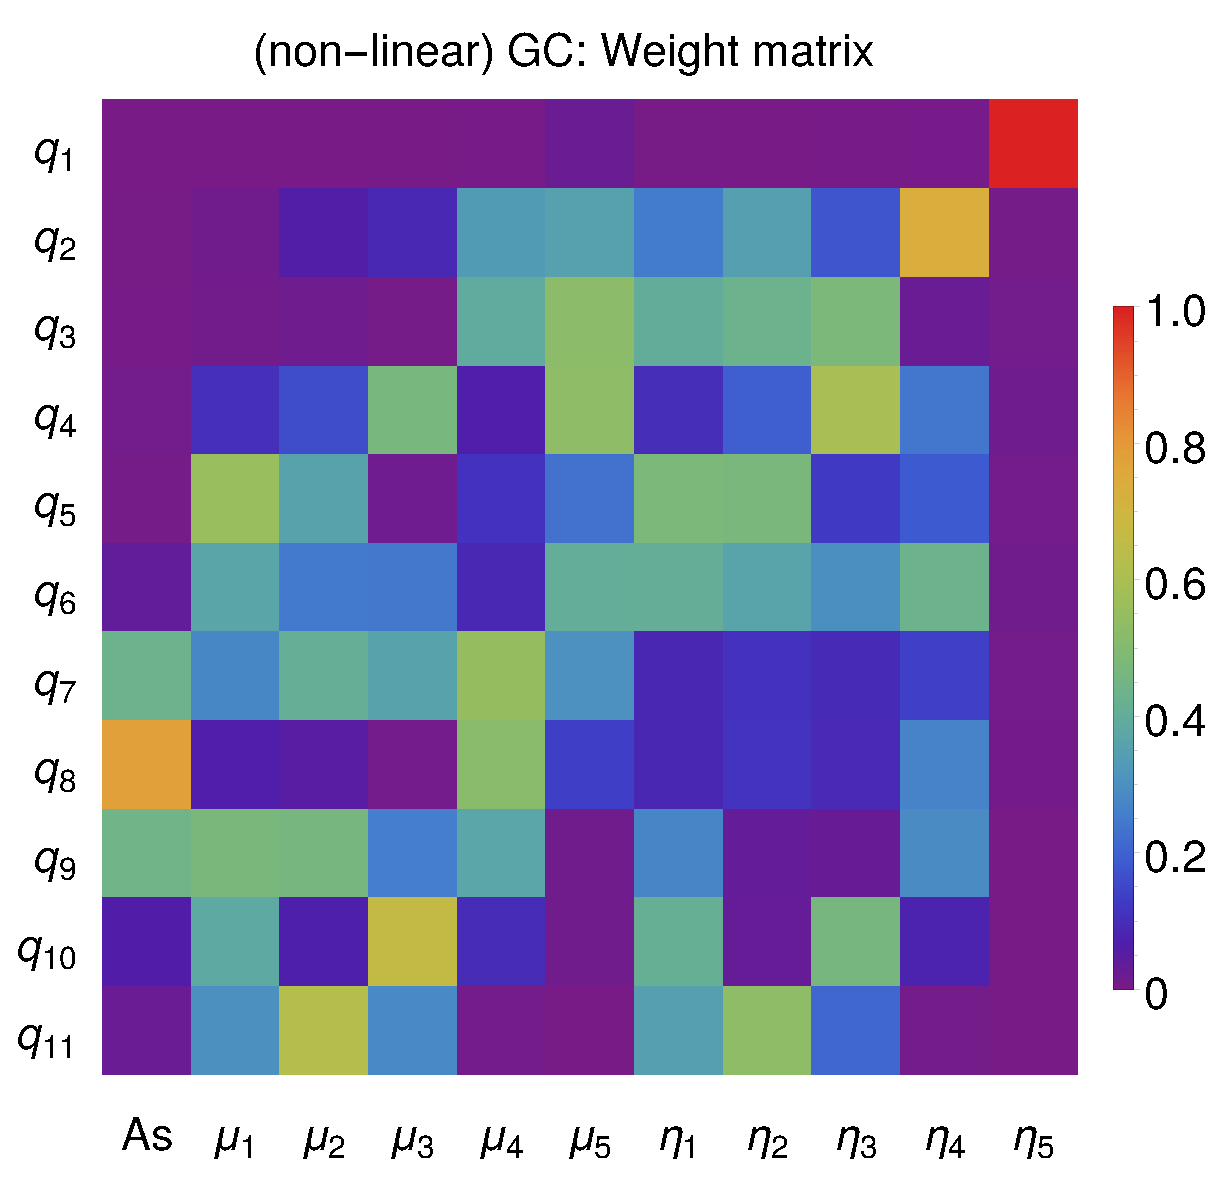
\includegraphics[width=0.47\textwidth]{Chapters/linear-nonlinear-MG-forecasts/figures/Decorrelations-GC/Weight_Matrix_PCA_SquareNorm--_fiducialMGBin3_Euclid_GC_nonlinearPk__Zhao_.pdf}
	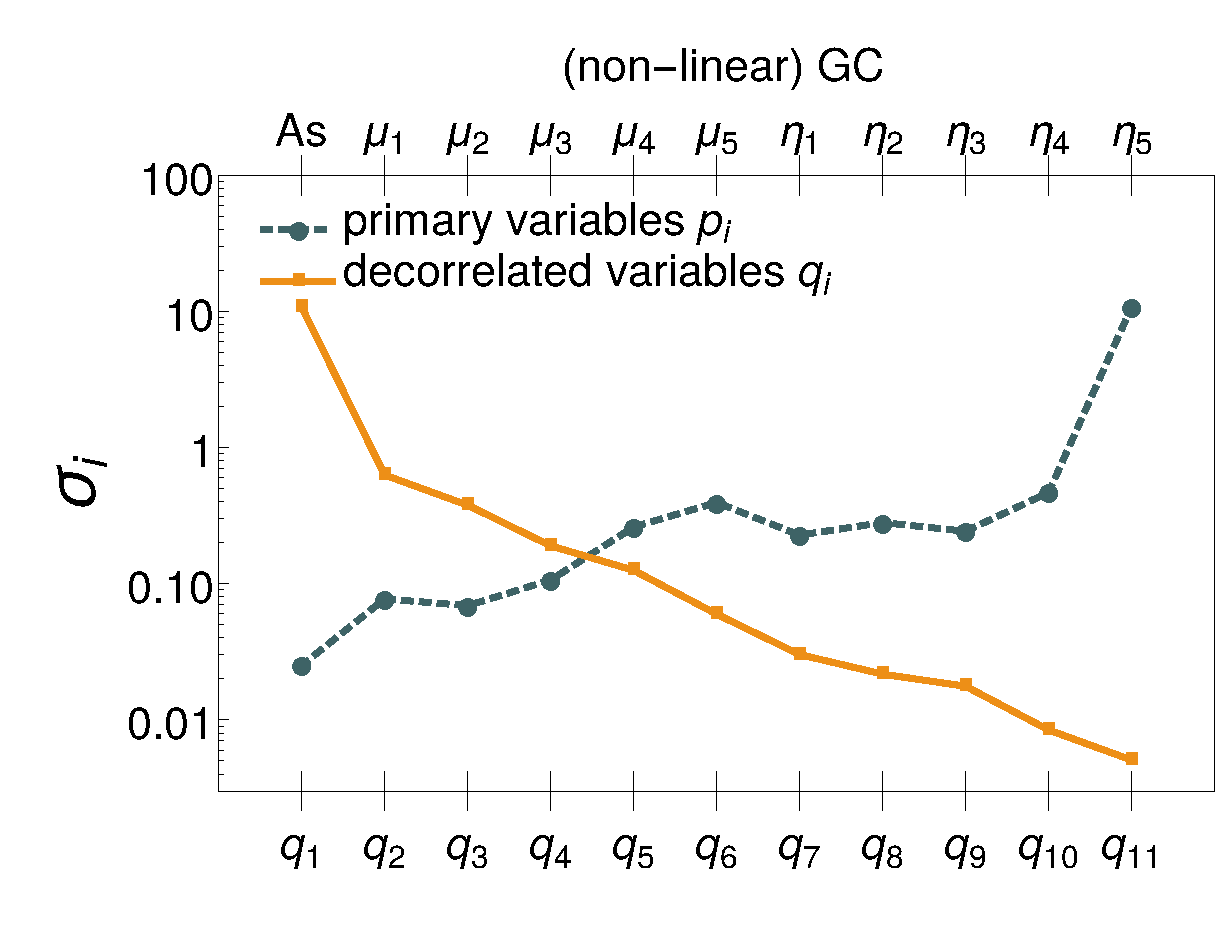
\includegraphics[width=0.47\textwidth]{Chapters/linear-nonlinear-MG-forecasts/figures/Decorrelations-GC/Errors_at_par_index_i--_PCA_SquareNorm--fiducialMGBin3_Euclid_GC_nonlinearPk__Zhao_.pdf}
	\caption[PCA decorrelation: Weight matrix and uncorrelated errors.]{\textbf{Left}: weight matrix $W$ for PCA. \textbf{Right}: 1$\sigma$ fully maximized errors on
		the primary parameters $p$ (blue lines) and the errors on the uncorrelated
		derived parameters $q$ (orange lines). Notice how all the important information is constrained in as few variables as possible,
		namely the last elements of $q_i$.
	}\label{fig:PCA-GCnlhs}
\end{figure}


\subsubsection{Cholesky decomposition}

Cholesky decomposition of the Fisher matrix $F=LL^{T}$, allows us to
define a decorrelation method that compresses
all components of $p$ into an upper triangular matrix of components
of $q$. This is achieved by using the $W$ matrix:

\begin{equation}
W=L^{T}
\end{equation}
Then the covariance matrix will be whitened:
\begin{align}
\tilde{C} & =L^{T} (L L^{T})^{-1} L\\
& =L^{T} (L^{T})^{-1} L^{-1} L\\
& =\mathbbm{1}
\end{align}
As done previously, we renormalize $W$ in such a way that the sum of the square of the elements of each row sum up to
unity.
In Cholesky decomposition, since we are constructing it via an upper triangular matrix (see left panel of Fig.\ \ref{fig:Chol-GCnlhs}), 
the new parameter $q_{11}$ will be identical 
to the parameter $\eta_5$, which is, as we have seen before (section \ref{subsub:ZCA-GC}), the less constrained parameter. This decorrelation method
is useful if one wants to have an ordering of the variables (see \cite{kessy_optimal_2015} and references therein).
On the other hand $q_1$ is almost identical to $A_s$, since as we have seen in section \ref{subsub:ZCA-GC},
it becomes decorrelated from the MG parameters in the non-linear case.

\begin{figure}[htbp]
	\centering 
	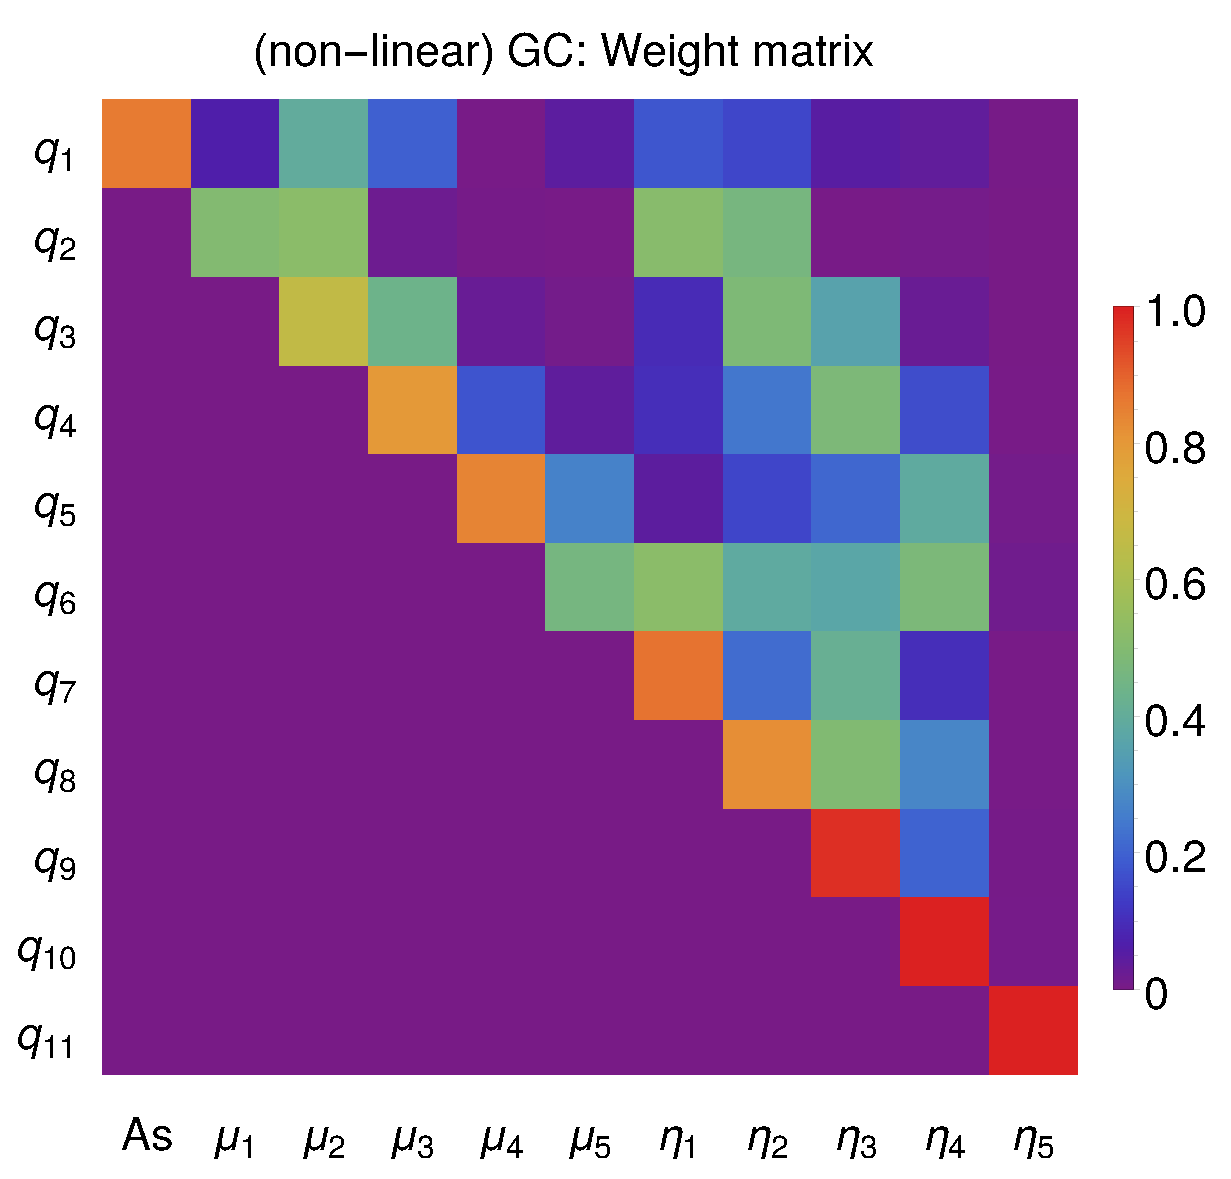
\includegraphics[width=0.47\textwidth]{Chapters/linear-nonlinear-MG-forecasts/figures/Decorrelations-GC/Weight_Matrix_Cholesky_SquareNorm--_fiducialMGBin3_Euclid_GC_nonlinearPk__Zhao_.pdf}
	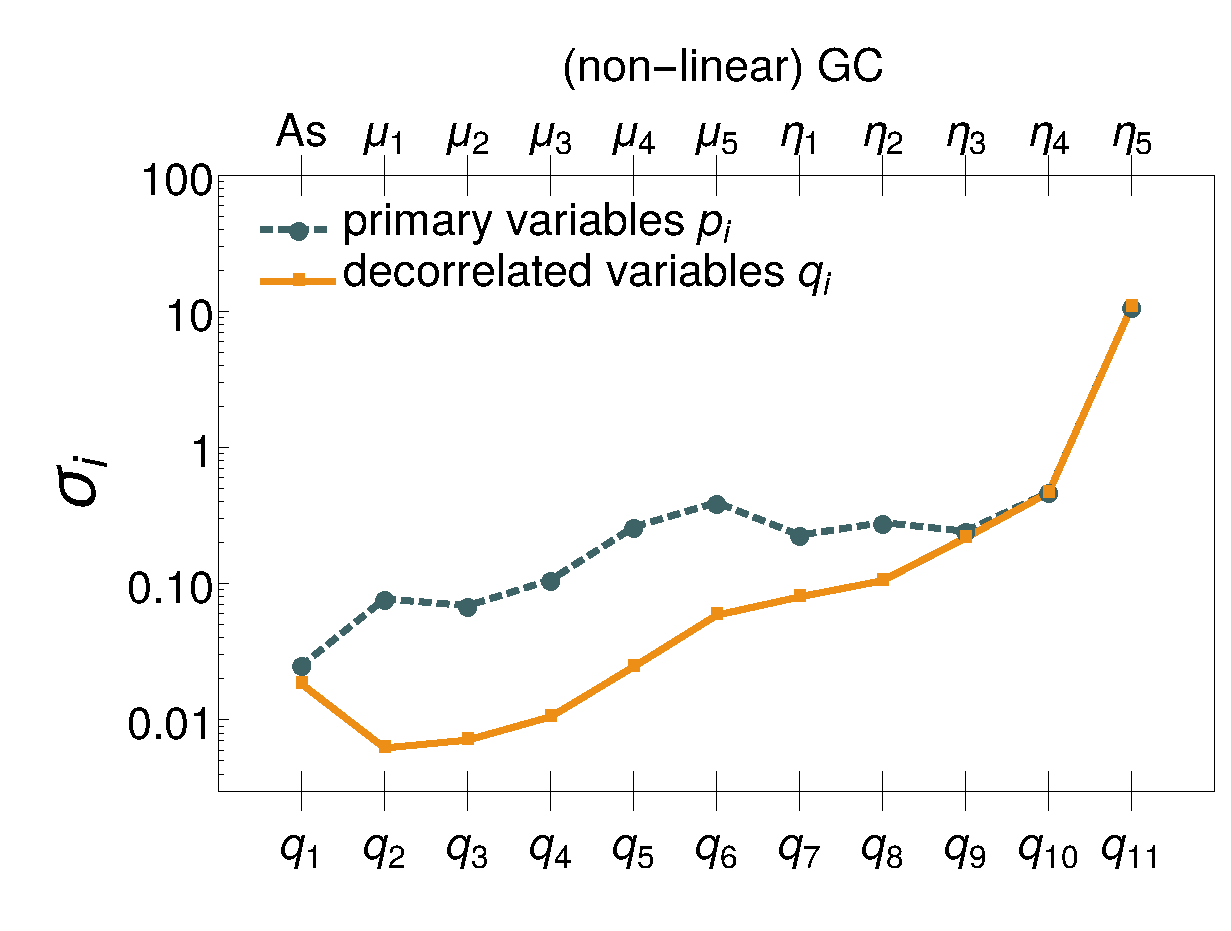
\includegraphics[width=0.47\textwidth]{Chapters/linear-nonlinear-MG-forecasts/figures/Decorrelations-GC/Errors_at_par_index_i--_Cholesky_SquareNorm--fiducialMGBin3_Euclid_GC_nonlinearPk__Zhao_.pdf}
	\caption[Cholesky decorrelation: Weight matrix and uncorrelated errors.]{\textbf{Left:} weight matrix $W$ for the Cholesky decorrelation. \textbf{Right:} 1$\sigma$ fully maximized errors on
		the primary parameters $p$ (blue lines) and the errors on the uncorrelated
		derived parameters $q$ (orange lines). Notice how in this case, because of the upper triangular construction, the new variables
		$q_{9,10,11}$ are equivalent to $\eta_{3,4,5}$. The parameter $A_s$ is decorrelated in the non-linear HS case for GC, therefore
		it is almost equivalent to $q_1$ as was also the case in ZCA (compare with Fig.\ \ref{fig:Wmat-ZCA-GC})
	}\label{fig:Chol-GCnlhs}
\end{figure}


\subsection{Kullback-Leibler divergence measure \label{sub:KL-matrices-MGBin}}

In \cref{sub:KL-def} we introduced the Kullback-Leibler divergence (see \cref{eq:KL-Gaussian}) as another way of measuring 
the constraining power of a survey and we defined the Kullback-Leibler matrices (\cref{eq:KL-Matrix}) (first introduced in \cite{casas_linear_2017}) as a way
of visualizing the information gain between different probes.
Here we will visualize the KL-matrix for the probes: GC(lin), GC(nl-HS), WL(lin), WL(nl-HS), GC+WL(lin) and GC+WL(nl-HS) in the redshift
binned parameterization of section \ref{sec:Results:-Redshift-Binned}.
In this way we can quantitatively see how much information is gained when going from one probe like Galaxy Clustering 
to another probe like Weak Lensing. 
In Figure \ref{fig:kl-matrices} we plot in the left panel the KL matrix $\mathcal{K}_{ij}$ when no \planck\ priors are added and 
in the right panel the KL matrix when \planck\ priors are added to all probes. 
For visualization purposes, 
we plot the logarithm of the KL matrix: $\log_{10} \mathcal{K}_{ij}$. 
Blue (red) colours represent small (large) information gain, while
black represents no information gain at all, which is by construction the case on the diagonal, $\mathcal{K}_{ii}=0$. 
The rows of the matrix represent the reference observable of $p_1$ and the columns,
the new observable $p_2$.
The information gain when going from a linear WL observable to a non-linear GC observable or to a combined GC+WL (linear and non-linear) 
observable is considerably high at about $\approx 10^6$-$10^7$. 
However, when adding a \planck\ prior, this gets reduced by at least 2 orders of magnitude, 
since the prior is strong and then there is not as much new information gained in the new observables. 
On the opposite case, we can see that the row corresponding to GC+WL(nl-HS) is mostly blue, 
meaning that there is little gain of information when going to one of the other observables.

\begin{figure}[h]
	\centering
	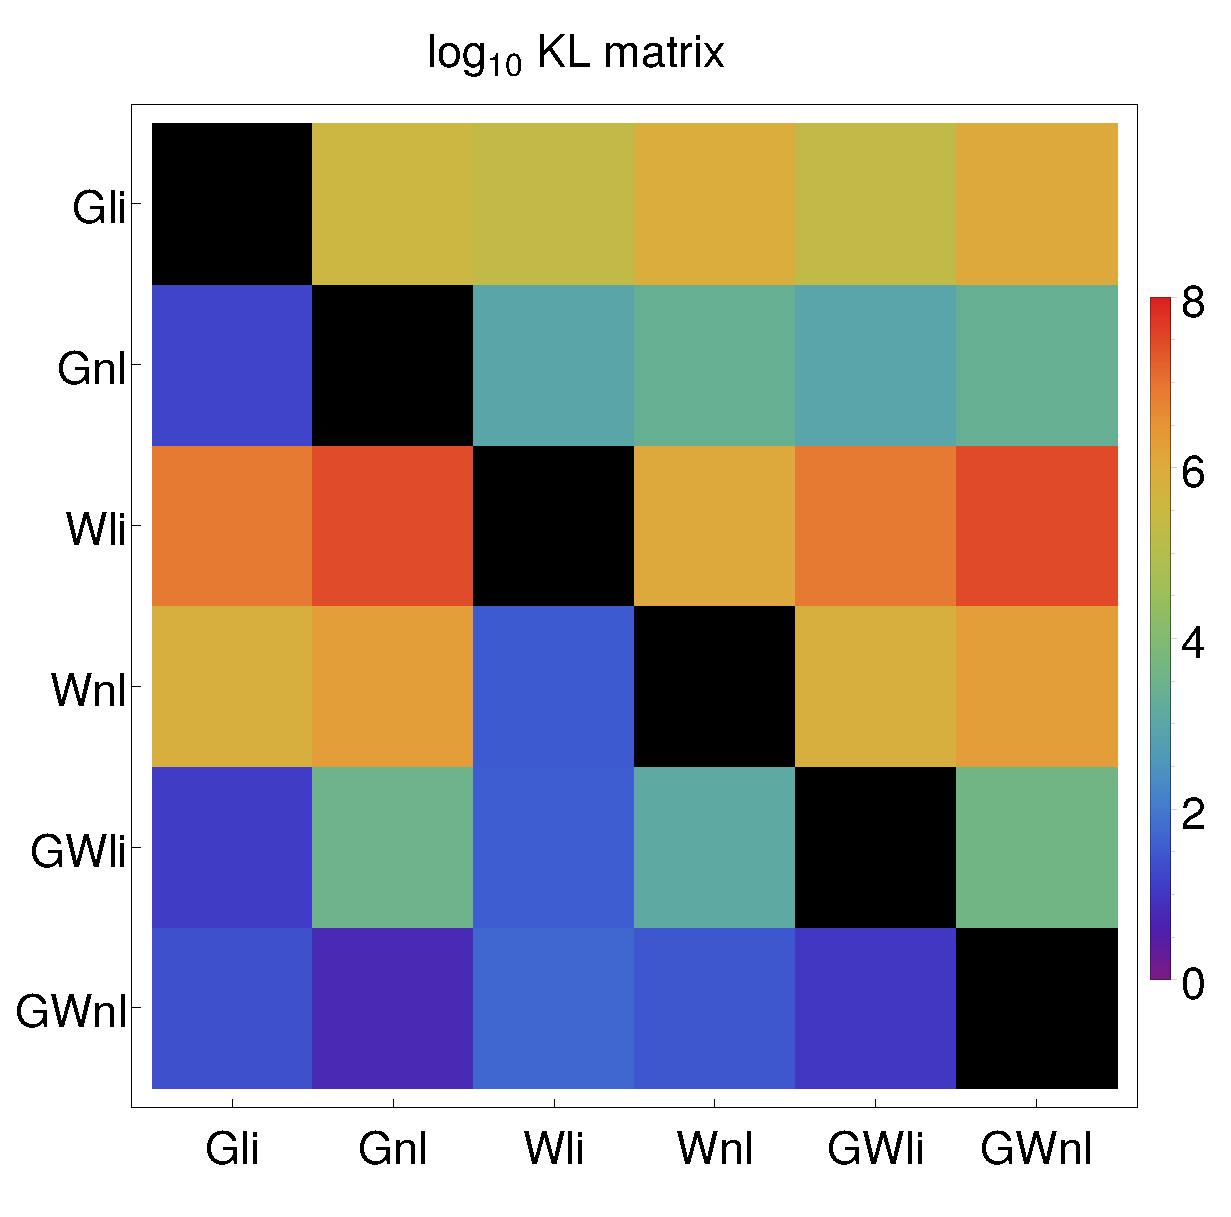
\includegraphics[width=0.47\linewidth]{Chapters/linear-nonlinear-MG-forecasts/figures/KL-divergence/KL-Matrix-all-obs-noPlanck-new}
	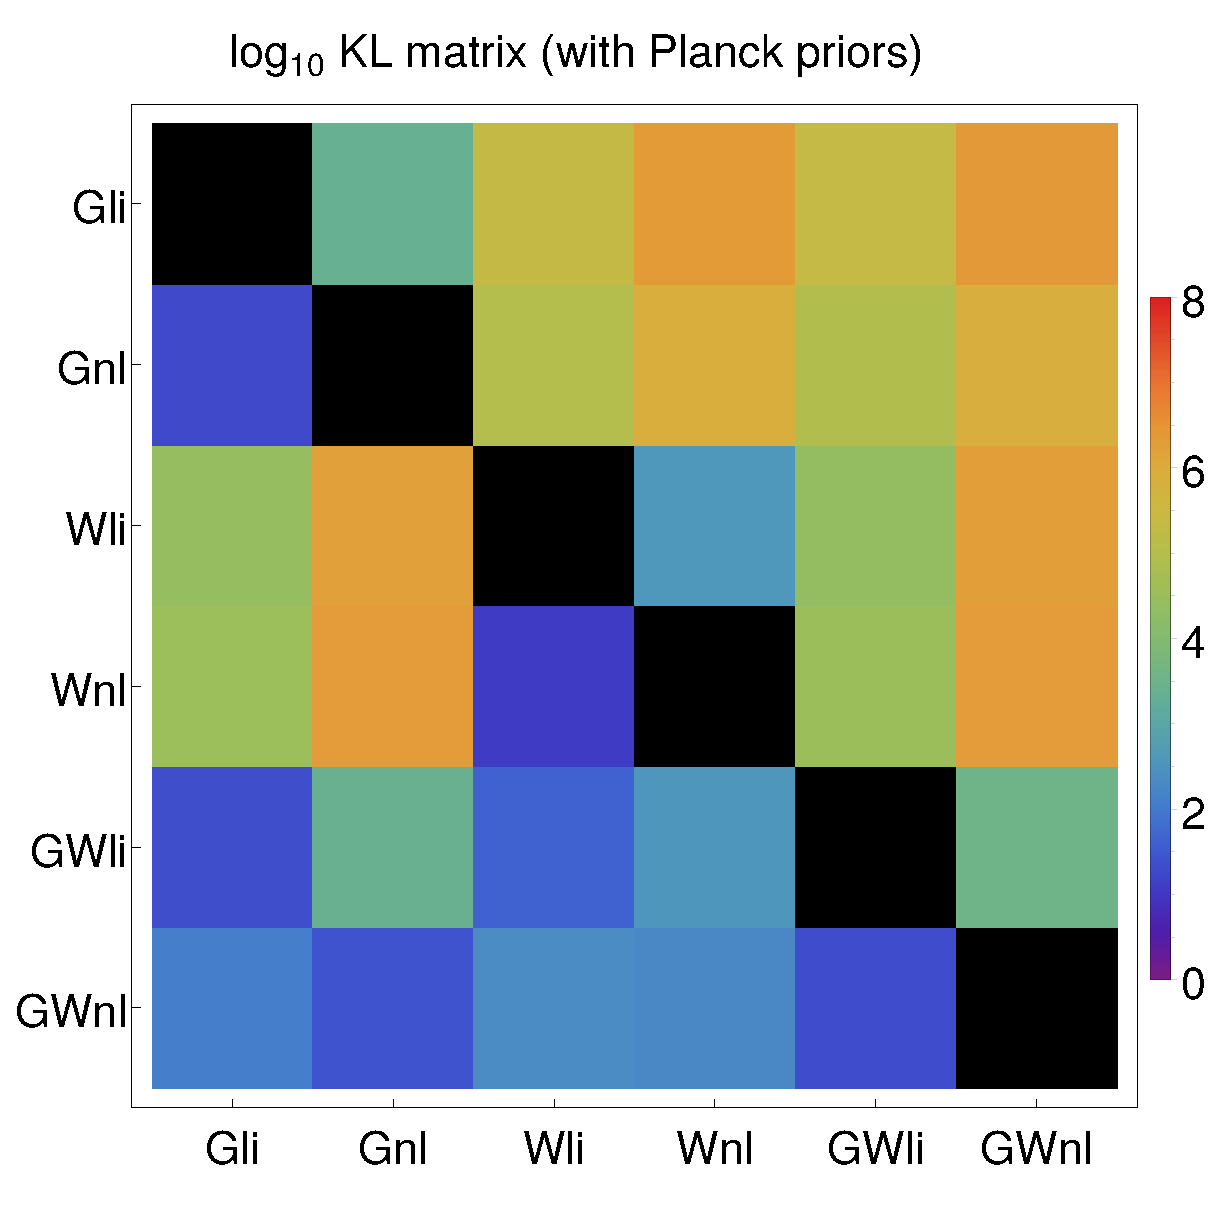
\includegraphics[width=0.47\linewidth]{Chapters/linear-nonlinear-MG-forecasts/figures/KL-divergence/KL-Matrix-all-obs-withPlanck-new}
	\caption[Kullback-Leibler divergence matrices for Euclid forecasts.]{Kullback-Leibler divergence matrices $\mathcal{K}_{ij}$. This matrix represents graphically
		the information gain between all possible observables in the redshift
		binned parameterization of section \ref{sec:Results:-Redshift-Binned}. 
		We have plotted here the logarithm of the KL-divergence matrix, for illustrative purposes. 
		Therefore the diagonal is $-\infty$ and it is represented by a black color. 
		\textbf{Left:} KL matrix without \planck\ priors. 
		The maximum gain is about $10^7$ when going from WL(lin) to GC+WL(non-linear) 
		and we can observe that GC+WL does not gain extra information when complemented with the other observables, which is expected.
		\textbf{Right:} In this case we compare the observables, when a \planck\ prior is added beforehand. 
		The overall information gain is now smaller, with a maximum of about $10^6$. 
		The maximum gain comes when comparing WL (linear and non-linear) to GC and GC+WL (non-linear). 
	}
	\label{fig:kl-matrices}
\end{figure}



\section{Modified gravity with simple smooth functions of the scale factor}

As discussed in \cref{sub:parameterizing-MG}, $\mu$ and $\eta$ (or an equivalent pair of functions of the gravitational potentials) depend in general on time and space. We will now investigate the time dependence further, starting from the two parameterizations proposed in \cite{planck_collaboration_planck_2016-7} and recalled in eqns.\ (\ref{eq:DE-mu-parametrization}-\ref{eq:TR-eta-parametrization}) in this work. We extend the analysis of the \planck\ paper \cite{planck_collaboration_planck_2016-7} by testing different prescriptions for the non-linear regime in Modified Gravity (as illustrated in Section \ref{sec:The-non-linear-power}) and further investigate forecasts for future experiments like Euclid, SKA, DESI. In the following subsections we first give results for the late-time parameterization of Eqns.\ (\ref{eq:DE-mu-parametrization},\ref{eq:DE-eta-parametrization}) and then for the early time parameterization of Eqns.\ (\ref{eq:TR-mu-parametrization},\ref{eq:TR-eta-parametrization}). In both cases we consider Galaxy Clustering and Weak Lensing, neglecting, as in Section \ref{sec:Results:-Redshift-Binned} any information coming from the cross correlation of the two probes.

\subsection{\label{sub:MG-DE}Modified Gravity in the late-time parameterization}

The late-time parameterization is defined in  \crefrange{eq:DE-mu-parametrization}{eq:DE-eta-parametrization}. We now calculate forecasts for Galaxy Clustering and Weak Lensing, with future surveys, in the linear and mildly non-linear regimes.
We also include prior information obtained from
the analysis of the {\it Planck}+BSH datasets (where we recall that BSH stands for BAO + SNe + $H_0$ prior),
as discussed in Section \ref{sub:Fisher-Planck}.

\subsubsection{Galaxy Clustering in the linear and mildly non-linear regime}

\done\todo[Maybe]{maybe add the correlation matrices for these models}
In Table \ref{tab:errors-Euclid-GC-WL-late_time} we show forecasts for the Euclid survey \cite{laureijs_euclid_2011} for Galaxy Clustering (top part of the table) and three different cases: using only linear scales with a cutoff at $k_{\rm max}=0.15$h/Mpc, labeled GC(lin); extending forecasts in the mildly non-linear regime, obtained using the prescription described in Sec.\ \ref{sub:Prescription-HS}, with a cutoff at $k_{\rm max}=0.5$ h/Mpc, labeled GC(nl-HS); combining the mildly non-linear case with \planck\ priors, as described in Sec.\ \ref{sub:Fisher-Planck}. We take into account
the BAO features, redshift space distortions and the full shape of
the power spectrum, as well as the survey specifications of the Euclid Redbook, recalled
in Section \ref{sub:Fisher-Galaxy-Clustering} for convenience. The columns correspond to the marginalized errors on five standard cosmological parameters $\{\Omega_c, \Omega_b, n_s, \ln (10^{10} A_s), h\}$ and three combinations of the gravitational potentials $\{\mu, \eta, \Sigma\}$: the latter are reconstructed in time, according to the late-time parameterization, as defined in Eqns.\ (\ref{eq:DE-mu-parametrization},\ref{eq:DE-eta-parametrization}). We recall that only two of these three functions are independent and fully determine cosmological linear perturbations.

In the late-time scenario, for a Galaxy Clustering survey,  
neither $\eta$ nor $\Sigma$ are actually
constrained by a linear forecast, while $\mu$ is mildly constrained.  
Adding the non-linear regime improves constraints on $\mu$, while the other parameters remain unconstrained, 
unless we also include \planck\ priors, which yields an improvement in the FoM of 6.3 nits. In general the observable power spectrum may depend on both $\mu$ (explicitely appearing in the last term of the equation for the density perturbation (cf. \cref{eq:dotdotdelta-mueta}) and on $\eta$ (implicitly contained in the derivatives of the gravitational potential in the same equation). The contribution of the derivative of the potentials is larger in the early-time parameterization, with respect to the late-time one by construction. This is due to the fact that in the late-time case deviations from GR go to zero at large redshifts. In this sense, in the specific case of the late time parameterization, the observed power spectrum mainly depends on $\mu$ only, which explains why this is the only quantity (mildly) constrained by GC alone. In the early-time parameterization, though, modifications can appear also at earlier times, so that both $\eta$ and $\mu$ effectively affect the power spectrum, which explains why they can both be constrained with a smaller uncertainty, as we will discuss in Section \ref{sub:MG-TR}.

In \cref{sec:appder} we review the equation governing the evolution of cold dark matter density fluctuations, 
as a function of the Modified Gravity functions $\mu(a)$ and $\eta(a)$ as they are implemented in the code MGCAMB \cite{hojjati_testing_2011}.
The inability of GC to constrain $\eta$ in this parametrization, is also visible in Fig.\ \ref{fig:DE+Planck-ellipses-mu-sig-eta} which shows that the GC constraints are
degenerate along the $\eta$ or $\Sigma$ directions.
Therefore, we show how with this parameterization choice Euclid GC will be extremely sensitive to
modifications of the Poisson equation for $\Psi$, while it would require additional
information to constrain departures from the standard Weyl potential.



\begin{table}[htbp]
\footnotesize
\begin{tabular}{|l|c|c|c|c|c||c|c|c|c|}
\hline 
\textbf{Euclid} (Redbook) & $\Omega_{c}$  & $\Omega_{b}$  & $n_{s}$  &
$\ell\mathcal{A}_{s}$  & $h$  & $\mu$  & $\eta$  & $\Sigma$ & MG FoM
\Tstrut\tabularnewline
\hline 
\multicolumn{1}{|l|}{Fiducial}   & {0.254}  & {0.048}  & {0.969}  & { 3.060}  & {0.682 } & {1.042}  & {1.719}  & {1.416} & relative \Tstrut\tabularnewline
\hline
\hline
\Tstrut \textbf{GC(lin)
}  
& 1.9\% & 6.4\% & 3\% & 2.8\% & 4.5\% & 17.1\% & 1030\% & 641\%
& 0\tabularnewline
\Tstrut\textbf{GC(nl-HS) 
}  
& 0.9\% & 2.5\% & 1.3\% & 0.8\% & 1.7\% & 1.7\% & 475\% & 291\%
& 2.9 \tabularnewline
\Tstrut\textbf{GC(nl-HS)+{\it Planck} 
}  
& 0.7\% & 0.6\% & 0.3\% & 0.2\% & 0.3\% & 1.7\% & 16.8\% & 10.3\%
& 6.3 \tabularnewline
\hline 
\hline
\Tstrut \textbf{WL(lin) 
}  
& 7.8\% & 25.7\% & 9.9\% & 10.3\% & 19.1\% & 58.2\% & 106\% & 9.3\%
& 3.2\tabularnewline
\Tstrut \textbf{WL(nl-HS) 
}    
& 6.3\% & 20.7\% & 4.6\% & 5.8\% & 13.8\% & 23.3\% & 40.9\% & 4.6\%
& 4.5 \tabularnewline
\Tstrut \textbf{WL(nl-HS)+{\it Planck} 
}  
& 2.1\% & 1.1\% & 0.4\% & 0.7\% & 0.7\% & 11.8\% & 21.8\% & 2.8\%
& 5.7 \tabularnewline
\hline
\hline
 \Tstrut \textbf{GC+WL(lin)}  
 & 1.8\% & 5.9\% & 2.8\% & 2.3\% & 4.2\% & 7.1\% & 10.6\% & 2\%
& 6.6 \tabularnewline
\Tstrut \textbf{GC+WL(lin)+{\it Planck}} $\;$  
 & 1.0\% & 0.7\% & 0.4\% & 0.4\% & 0.4\% & 6.2\% & 9.8\% & 1.5\%
& 7.0  \tabularnewline
\hline
\hline
 \Tstrut \textbf{GC+WL(nl-HS)}  
 & 0.8\% & 2.2\% & 0.8\% & 0.7\% & 1.5\% & 1.6\% & 2.4\% & 1.0\%
& 8.8 \tabularnewline
\Tstrut \textbf{GC+WL(nl-HS)+{\it Planck}} $\;$  
 & 0.7\% & 0.6\% & 0.2\% & 0.2\% & 0.3\% & 1.6\% & 2.4\% & 0.9\%
& 8.9  \tabularnewline
\Tstrut \textbf{GC+WL(nl-Halofit)+{\it Planck}} $\;$ 
& 0.6\% & 0.5\% & 0.2\% & 0.2\% & 0.2\% & 0.8\% & 1.7\% & 0.8\%
& 9.6  \tabularnewline
\hline  
\end{tabular}\protect
\small
\caption[1$\sigma$ marginalized errors for a Euclid GC and WL forecast in the late-time parameterization.]{\label{tab:errors-Euclid-GC-WL-late_time}
1$\sigma$
fully marginalized errors on the cosmological parameters in the late-time parameterization of Modified Gravity for a Euclid
Galaxy Clustering forecast (top), a Weak Lensing forecast (middle) and the combination
of both probes (bottom): 
Modified Gravity is encoded in two of the three functions $\mu$, $\eta$, $\Sigma$, 
which are reconstructed in the late-time parameterization defined in 
Eqns.\ (\ref{eq:DE-mu-parametrization},\ref{eq:DE-eta-parametrization}). For each case, we also list
the forecasted errors using a {\it Planck}+BSH prior.
Linear forecasts are labeled by ``lin'', and correspond to a cutoff $k_{\rm max}=0.15$h/Mpc for GC and $\ell_{\rm max}=5000$ for WL; 
non-linear forecasts use the prescription described in 
sec.\ \ref{sub:Prescription-HS}, are labeled by ``nl-HS'' and correspond to a cutoff of $k_{\rm max}=0.5$h/Mpc for GC and $\ell_{\rm max}=5000$ for WL.
in both cases, power spectra have been computed using the MGCAMB Boltzmann code. For completeness,
we also show the GC+WL+{\it Planck} case using the non-linear power spectra computed using Halofit only (nl-Halofit).
In the last column, we show for each observation the Figure of Merit (FoM) 
relative to our base observable in this parametrization, which is GC(linear).
GC(linear) has an absolute FoM of -0.94 in `nits'.
We can see that in both GC and WL there is a considerable gain when including non-linear scales and \planck\ priors.
The difference in the FoM between the non-linear HS prescription and the standard Halofit approach
is quite small. 
}
\end{table}
\normalsize

\begin{table}[htbp]
\footnotesize
\centering{}
\begin{tabular}{|l|c|c|c|c|c||c|c|c|c|}
\hline
\Tstrut \textbf{Euclid} (Redbook) & $\Omega_{c}$ & $\Omega_{b}$ & $n_{s}$ & $\ell\mathcal{A}_{s}$ & $h$ & $\mu$ & $\eta$ & $\Sigma$
& MG FoM  \tabularnewline
\hline 
\Tstrut Fiducial & {0.256} & {0.048} & {0.969} & {3.091} & {0.682} & {0.902} & {1.939} & {1.326} & relative\tabularnewline
\hline
\hline 
\Tstrut\textbf{GC(lin)} & 3.7\% & 19.2\% & 9.1\% & 16.6\% & 16.5\% & 16.7\% & 758\% & 489\%  
& 0 \tabularnewline
\Tstrut \textbf{GC(nl-HS)} & 1.1\% & 2.3\% & 1.3\% & 0.7\% & 1.6\% & 1.8\% & 7.9\% & 4.8\%
& 6.6 \tabularnewline 
\Tstrut \textbf{GC(nl-HS)+{\it Planck}}  & 0.8\% & 0.7\% & 0.3\% & 0.3\% & 0.3\% & 1.7\% & 7.6\% & 4.6\%
& 6.7 \tabularnewline
\hline 
\hline 
\Tstrut \textbf{WL(lin)}  & 12.1\% & 28.9\% & 11.3\% & 13.3\% & 24\% & 6.8\% & 11.1\% & 11.9\%
& 4.9 \tabularnewline 
\Tstrut \textbf{WL(nl-HS)}  & 6.5\% & 21.9\% & 6.6\% & 5.9\% & 15.8\% & 2.8\% & 8.0\% & 3.4\%
& 6.6  \tabularnewline
\Tstrut \textbf{WL(nl-HS)+{\it Planck}}  & 2.1\% & 1.3\% & 0.5\% & 0.9\% & 0.7\% & 2.2\% & 7.2\% & 2.9\%
& 7.2 \tabularnewline
\hline
\hline 
\Tstrut \textbf{GC+WL(lin)}  & 1.8\% & 6.6\% & 3.4\% & 5.6\% & 5.2\% & 3.0\% & 6.8\% & 3.4\%  
& 6.4  \tabularnewline
\Tstrut \textbf{GC+WL(lin)+{\it Planck}}  & 1.2\% & 0.9\% & 0.6\% & 2.3\% & 0.4\% & 2.4\% & 6.5\% & 2.8\%  
& 6.9  \tabularnewline
\hline
\hline 
\Tstrut \textbf{GC+WL(nl-HS)}  & 1.0\% & 2.2\% & 1.2\% & 0.7\% & 1.6\% & 1.3\% & 4.4\% & 1.9\% 
& 8.0   \tabularnewline
\Tstrut \textbf{GC+WL(nl-HS)+{\it Planck}}  & 0.8\% & 0.7\% & 0.3\% & 0.3\% & 0.3\% & 1.3\% & 4.4\% & 1.9\% 
& 8.2  \tabularnewline
\Tstrut \textbf{GC+WL(nl-Halofit)+{\it Planck} $\;$}  & 0.7\% & 0.7\% & 0.3\% & 1.3\% & 0.3\% & 0.9\% & 2.3\% & 1\% 
& 8.9  \tabularnewline
\hline
\end{tabular}
\small
\protect\caption[1$\sigma$ marginalized errors for a Euclid GC and WL forecast in the late-time parameterization.]{\label{tab:errors-Euclid-GC-WL-early_time}
Same as Table (\ref{tab:errors-Euclid-GC-WL-late_time}) but for the  early-time parameterization. Note that the last column (MG FoM) cannot be compared to the one for a different parameterization (Table \ref{tab:errors-Euclid-GC-WL-late_time}) since the reference value is different (GC(lin)) and the two parameterizations have a different number of primary parameters). In this case the absolute MG FoM of GC(lin) is $\approx -0.47$ nits.
}
\end{table}
\normalsize

\begin{table}[htbp]
\centering{}%
\footnotesize
\begin{tabular}{|l|c|c|c|c|c||c|c|c|c|}
	\hline
	 & $\Omega_{c}$ & $\Omega_{b}$ & $n_{s}$ & $\ell\mathcal{A}_{s}$ & $h$ & $\mu$ & $\eta$ & $\Sigma$ & MG FoM \TBstrut\tabularnewline
\hline 
Fiducial & {0.254 } & {0.048 } & {0.969 } & {3.060 } & {0.682 } & {1.042 } & {1.719 } & {1.416 } & relative\TBstrut\tabularnewline
\hline 
\hline 
\textbf{GC(nl-HS)} &  &  &  &  &  &  &  & & \TBstrut\tabularnewline
Euclid   
& 0.9\% & 2.5\% & 1.3\% & 0.8\% & 1.7\% & 1.7\% & 475\% & 291\%
& 2.9
\tabularnewline
SKA1-SUR  
& 5\% & 15.3\% & 8.7\% & 3.8\% & 10.8\% & 18.1\% & 165\% & 108\%
& 1.7
\tabularnewline
SKA2  
& 0.5\% & 1.3\% & 0.4\% & 0.4\% & 0.8\% & 0.7\% & 86.8\% & 53.2\%
& 5.5
\tabularnewline
DESI-ELG   
& 1.6\% & 4.1\% & 2.3\% & 1.3\% & 2.9\% & 3.3\% & 899\% & 552\%
& 1.8
\tabularnewline
\hline 
\hline 
\textbf{WL(nl-HS)} &  &  &  &  &  &  &  &  & \TBstrut\tabularnewline
Euclid   
& 6.3\% & 20.7\% & 4.6\% & 5.8\% & 13.8\% & 23.3\% & 40.9\% & 4.6\%
& 4.5
\tabularnewline
SKA1  
& 30.8\% & 109\% & 35\% & 36.5\% & 77.6\% & 220\% & 405\% & 36.8\%
& 0.5
\tabularnewline
SKA2  
& 6\% & 22.5\% & 5.9\% & 6.8\% & 15.9\% & 19\% & 33.2\% & 3.7\%
& 4.9
\tabularnewline
\hline 
\hline 
\textbf{GC+WL(lin)} &  &  &  &  &  &  &  & & \Tstrut\tabularnewline
Euclid  
& 1.8\% & 5.9\% & 2.8\% & 2.3\% & 4.2\% & 7.1\% & 10.6\% & 2\%
& 6.6
\tabularnewline
SKA1  
& 10.1\% & 47.6\% & 25.4\% & 21.7\% & 40.4\% & 26.4\% & 28.8\% & 13.6\%
& 3.7
\tabularnewline
SKA2 
& 1.2\% & 4.5\% & 2.2\% & 1.9\% & 3.3\% & 4.1\% & 5.5\% & 1.6\%
& 7.5
\tabularnewline
\hline 
\hline 
\textbf{GC+WL(lin)+{\it Planck}} &  &  &  &  &  &  &  & & \Tstrut\tabularnewline
Euclid  
& 1.0\% & 0.7\% & 0.4\% & 0.4\% & 0.4\% & 6.2\% & 9.8\% & 1.5\%
& 6.9
\tabularnewline
SKA1  
& 2.4\% & 1.2\% & 0.4\% & 1.2\% & 0.7\% & 12\% & 19.8\% & 3.8\%
& 5.3
\tabularnewline
SKA2 
& 0.7\% & 0.6\% & 0.3\% & 0.4\% & 0.3\% & 3.6\% & 5.2\% & 1.2\%
& 7.8
\tabularnewline
\hline 
\hline 
\textbf{GC+WL(nl-HS)} &  &  &  &  &  &  &  & & \Tstrut\tabularnewline
Euclid  
& 0.8\% & 2.2\% & 0.8\% & 0.7\% & 1.5\% & 1.6\% & 2.4\% & 1.0\%
& 8.7
\tabularnewline
SKA1  
& 4.7\% & 14.3\% & 6.2\% & 3.6\% & 9.6\% & 12.8\% & 11\% & 7.3\%
& 5.5
\tabularnewline
SKA2 
& 0.4\% & 1.3\% & 0.3\% & 0.4\% & 0.8\% & 0.7\% & 0.9\% & 0.6\%
& 10.3
\tabularnewline
\hline
\hline
\textbf{GC+WL(nl-HS)+{\it Planck}} &  &  &  &  &  &  &  & & \Tstrut\tabularnewline
Euclid  
& 0.7\% & 0.6\% & 0.2\% & 0.2\% & 0.3\% & 1.6\% & 2.4\% & 0.9\%
& 8.9
\tabularnewline 
SKA1  
& 2.0\% & 1.0\% & 0.4\% & 0.8\% & 0.6\% & 3.5\% & 6\% & 2.7\%
& 6.9
\tabularnewline 
SKA2 
& 0.4\% & 0.5\% & 0.2\% & 0.1\% & 0.2\% & 0.6\% & 0.9\% & 0.5\%
& 10.3
\tabularnewline
\hline
\end{tabular}
\small
\protect\caption[1$\sigma$ marginalized errors for Euclid, DESI-ELG, SKA1 and SKA2 forecasts in the late-time parameterization.]{\label{tab:errors-GC-SKAcompare-MG-DE-mu-eta-sigma}
1$\sigma$ fully
marginalized errors on the cosmological parameters
$\{\Omega_{m},\Omega_{b},h,\ell \mathcal{A}_{s},n_{s},\mu,\eta, \Sigma\}$
in the late-time parameterization comparing different surveys in the linear and non-linear case. 
In the last column, we show for each observation the Modified Gravity Figure of Merit (MG FoM) relative to our base observable, which is the Euclid Redbook GC(linear), see Table \ref{tab:errors-Euclid-GC-WL-late_time}.
We can see that in general terms, SKA2 is the most powerful survey, followed by Euclid and SKA1.
In the case of GC alone, DESI-ELG is more constraining than SKA1-SUR.
Notice that in this parameterization, a GC survey would only constrain $\mu$ with
a high accuracy, while a WL survey would constrain $\Sigma$ with
a very good accuracy. The combination of both is much more
powerful than the single probes. Adding \planck\ priors (last row) improves considerably the
constraints on the $\lcdm$ parameters but has an almost negligible effect on the MG parameters (MG FoM remain almost constant when adding \planck\ priors to the GC+WL (non-linear HS) case. The marginalized contours for the $\mu$-$\eta$ plane , comparing these surveys, can be seen in the left panel of \cref{fig:combined_surveys}.
}
\end{table}


\begin{table}[htbp]
\centering{}%
\footnotesize
\begin{tabular}{|l|c|c|c|c|c||c|c|c|c|}
\hline
	 & $\Omega_{c}$ & $\Omega_{b}$ & $n_{s}$ & $\ell\mathcal{A}_{s}$ & $h$ & $\mu$ & $\eta$ & $\Sigma$  & MG FoM \TBstrut\tabularnewline
\hline 
Fiducial & {0.256} & {0.0485} & {0.969} & {3.091} & {0.682} & {0.902} & {1.939} & {1.326} & relative \TBstrut\tabularnewline 
\hline 
\hline 
\textbf{GC(nl-HS)} &  &  &  &  &  &  &  & & \TBstrut\tabularnewline
Euclid   
& 1.1\% & 2.3\% & 1.3\% & 0.7\% & 1.6\% & 1.8\% & 7.9\% & 4.8\%
& 6.6
\tabularnewline
SKA1-SUR  
& 7.9\% & 14.2\% & 13.4\% & 4.2\% & 11\% & 12.6\% & 82.7\% & 52.6\%
& 2.2
\tabularnewline
SKA2  
& 0.6\% & 1.3\% & 0.7\% & 0.4\% & 0.9\% & 0.9\% & 3.4\% & 1.8\%
& 8.3
\tabularnewline
DESI-ELG   
& 2.0\% & 4.3\% & 2.7\% & 1.4\% & 3.0\% & 8.2\% & 32\% & 28.6\%
& 4.3
\tabularnewline
\hline 
\hline 
\textbf{WL(nl-HS)} &  &  &  &  &  &  &  &  & \TBstrut\tabularnewline
Euclid   
& 6.5\% & 21.9\% & 6.6\% & 5.9\% & 15.8\% & 2.8\% & 8.0\% & 3.4\%
& 6.6
\tabularnewline
SKA1  
& 32\% & 106\% & 37.2\% & 33\% & 79.3\% & 13.1\% & 37.1\% & 16.4\%
& 3.4
\tabularnewline
SKA2  
& 5.9\% & 22.1\% & 6.7\% & 6.1\% & 16.1\% & 2.4\% & 7.0\% & 2.9\%
& 6.9
\tabularnewline
\hline 
\hline 
\textbf{GC+WL(lin)} &  &  &  &  &  &  &  & & \Tstrut\tabularnewline
Euclid  
& 1.8\% & 6.6\% & 3.4\% & 5.6\% & 5.2\% & 3.0\% & 6.8\% & 3.4\%
& 6.4
\tabularnewline
SKA1  
& 10.3\% & 46.4\% & 24.2\% & 33.6\% & 40.2\% & 14.4\% & 29.6\% & 15.5\%
& 3.3
\tabularnewline
SKA2 
& 1.3\% & 4.9\% & 2.5\% & 4.2\% & 3.9\% & 2.5\% & 5.7\% & 2.7\%
& 6.8
\tabularnewline
\hline 
\hline 
\textbf{GC+WL(lin)+{\it Planck}} &  &  &  &  &  &  &  & & \Tstrut\tabularnewline
Euclid  
& 1.2\% & 0.9\% & 0.6\% & 2.3\% & 0.4\% & 2.4\% & 6.5\% & 2.8\%
& 6.8
\tabularnewline
SKA1  
& 2.5\% & 1.5\% & 0.8\% & 2.9\% & 0.8\% & 8.8\% & 22.2\% & 8.5\%
& 4.5
\tabularnewline
SKA2 
& 0.9\% & 0.7\% & 0.6\% & 2.1\% & 0.3\% & 2.1\% & 5.4\% & 2.3\%
& 7.2
\tabularnewline
\hline 
\hline 
\textbf{GC+WL(nl-HS)} &  &  &  &  &  &  &  & & \Tstrut\tabularnewline
Euclid  
& 1.0\% & 2.2\% & 1.2\% & 0.7\% & 1.6\% & 1.3\% & 4.4\% & 1.9\%
& 8.1
\tabularnewline
SKA1  
& 7.1\% & 13.4\% & 10.7\% & 4\% & 10\% & 8.2\% & 24.4\% & 10.5\%
& 4.4
\tabularnewline
SKA2 
& 0.6\% & 1.3\% & 0.7\% & 0.4\% & 0.9\% & 0.8\% & 2.7\% & 1.3\%
& 8.8
\tabularnewline
\hline
\hline
\textbf{GC+WL(nl-HS)+{\it Planck}} &  &  &  &  &  &  &  & & \Tstrut\tabularnewline
Euclid  
& 0.8\% & 0.7\% & 0.3\% & 0.3\% & 0.3\% & 1.3\% & 4.4\% & 1.9\%
& 8.1
\tabularnewline 
SKA1  
& 2.1\% & 1.3\% & 0.5\% & 0.9\% & 0.7\% & 7\% & 20.8\% & 8.2\%
& 4.9
\tabularnewline 
SKA2 
& 0.5\% & 0.5\% & 0.3\% & 0.2\% & 0.2\% & 0.8\% & 2.7\% & 1.3\%
& 8.8
\tabularnewline
\hline
\end{tabular}
\small
\caption[1$\sigma$ marginalized errors for Euclid, DESI-ELG, SKA1 and SKA2 forecasts in the early-time parameterization.]{\label{tab:errors-GC-SKAcompare-MG-TR-mu-eta-sigma-Zhao-1}
Same as Table \ref{tab:errors-GC-SKAcompare-MG-DE-mu-eta-sigma} but for the early-time parameterization.
The last 4 columns correspond to the
projection of the errors on $E_{11}$ and $E_{22}$ onto $\mu,\;\eta$ and $\Sigma$, respectively. 
We have marginalized over $E_{12}$
and $E_{21}$ since at $z=0$ they don't contribute to the Modified
Gravity parameters. Notice that in this
parameterization, a GC survey alone is able to constrain both $\mu$ and $\Sigma$ to a good level for all surveys, better than with the late time parameterization, more often used in literature. The combination of GC+WL is however less constraining in the early time parametrization than in late time parameterization one. The reference case for the MG FoM is the Euclid (Redbook) GC linear forecast (Table \ref{tab:errors-Euclid-GC-WL-early_time}).
The non-linear forecast for GC+WL+{\it Planck} would yield, for Euclid and SKA2, contraints at the 1-2\% accuracy on $\mu$, $\Sigma$, while
for SKA1 the contraints would be at the 8\% level. The marginalized contours for the $\mu$-$\eta$ plane , comparing these surveys, can be seen in the right panel ofFig.\ref{fig:combined_surveys}.
}
\end{table}
\normalsize




\subsubsection{Weak Lensing in the linear and mildly non-linear regime}

Using the Euclid Weak Lensing specifications described in Section
sub:Fisher-Weak-Lensing, we obtain the results displayed in
the middle panel of Table \ref{tab:errors-Euclid-GC-WL-late_time}. 
Also in this case, we use the late-time parameterization, in three different cases: 
the first uses only linear quantities, with a maximum multipole of $\ell_{\rm max}=1000$; 
the second case uses the non-linear HS prescription of section \ref{sub:Prescription-HS} 
up to a maximum multipole of $\ell_{\rm max}=5000$; the third case combines Weak Lensing with \planck\ priors, 
as described in \ref{sub:Fisher-Planck}.

In the linear case, WL forecast yields constraints on the standard $\lcdm$ parameters
at around 10\% of accuracy, with the exception of $\Omega_{b}$ which
is poorly constrained at around 26\%, and the expansion rate h (19\%). This is likely due to the fact
that WL is only directly sensitive to the total matter distribution
in the Universe and cannot differentiate baryons from dark matter. All constraints improve when adding non-linear information, with $\Omega_b$ and h still constrained only at the level of about $20\%$. When the \planck\ priors are included, though, constraints shrink down to about 1$\%$ for all cosmological parameters.
The Modified Gravity parameters show the expected
trend; in the linear case, only $\Sigma$ is constrained, at 11$\%$, as this parameter is directly defined in terms of the lensing potential $\Phi+\Psi$; a Weak Lensing
probe is however not directly sensitive to $\mu$ and $\eta$ separately, as can be seen in Fig.\ \ref{fig:DE+Planck-ellipses-mu-sig-eta}.
The linear FoM is only slightly weaker than the one from GC for this parameterization, probably because both probes have an effectively unconstrained degeneracy direction. When adding non-linear information, errors on $\mu$ and $\eta$ improve, though still remaining in a poorly constrained interval (25$\%$-44$\%$).
Already on its own, however, Weak Lensing could rule out many
models of Modified Gravity that change $\Sigma$ at more than $5\%$ (or even $2.9\%$, if we include \planck\ priors). The combination GC+{\it Planck} 
and WL+{\it Planck} has a comparable overall constraining power, with GC+{\it Planck} being about 1 nit stronger and providing smaller errors on $\mu$.

\subsubsection{Combining Weak Lensing and Galaxy Clustering}\label{subsub:late-time-comb-GC+WL}

\begin{figure}[htbp]
	\centering
\begin{centering}
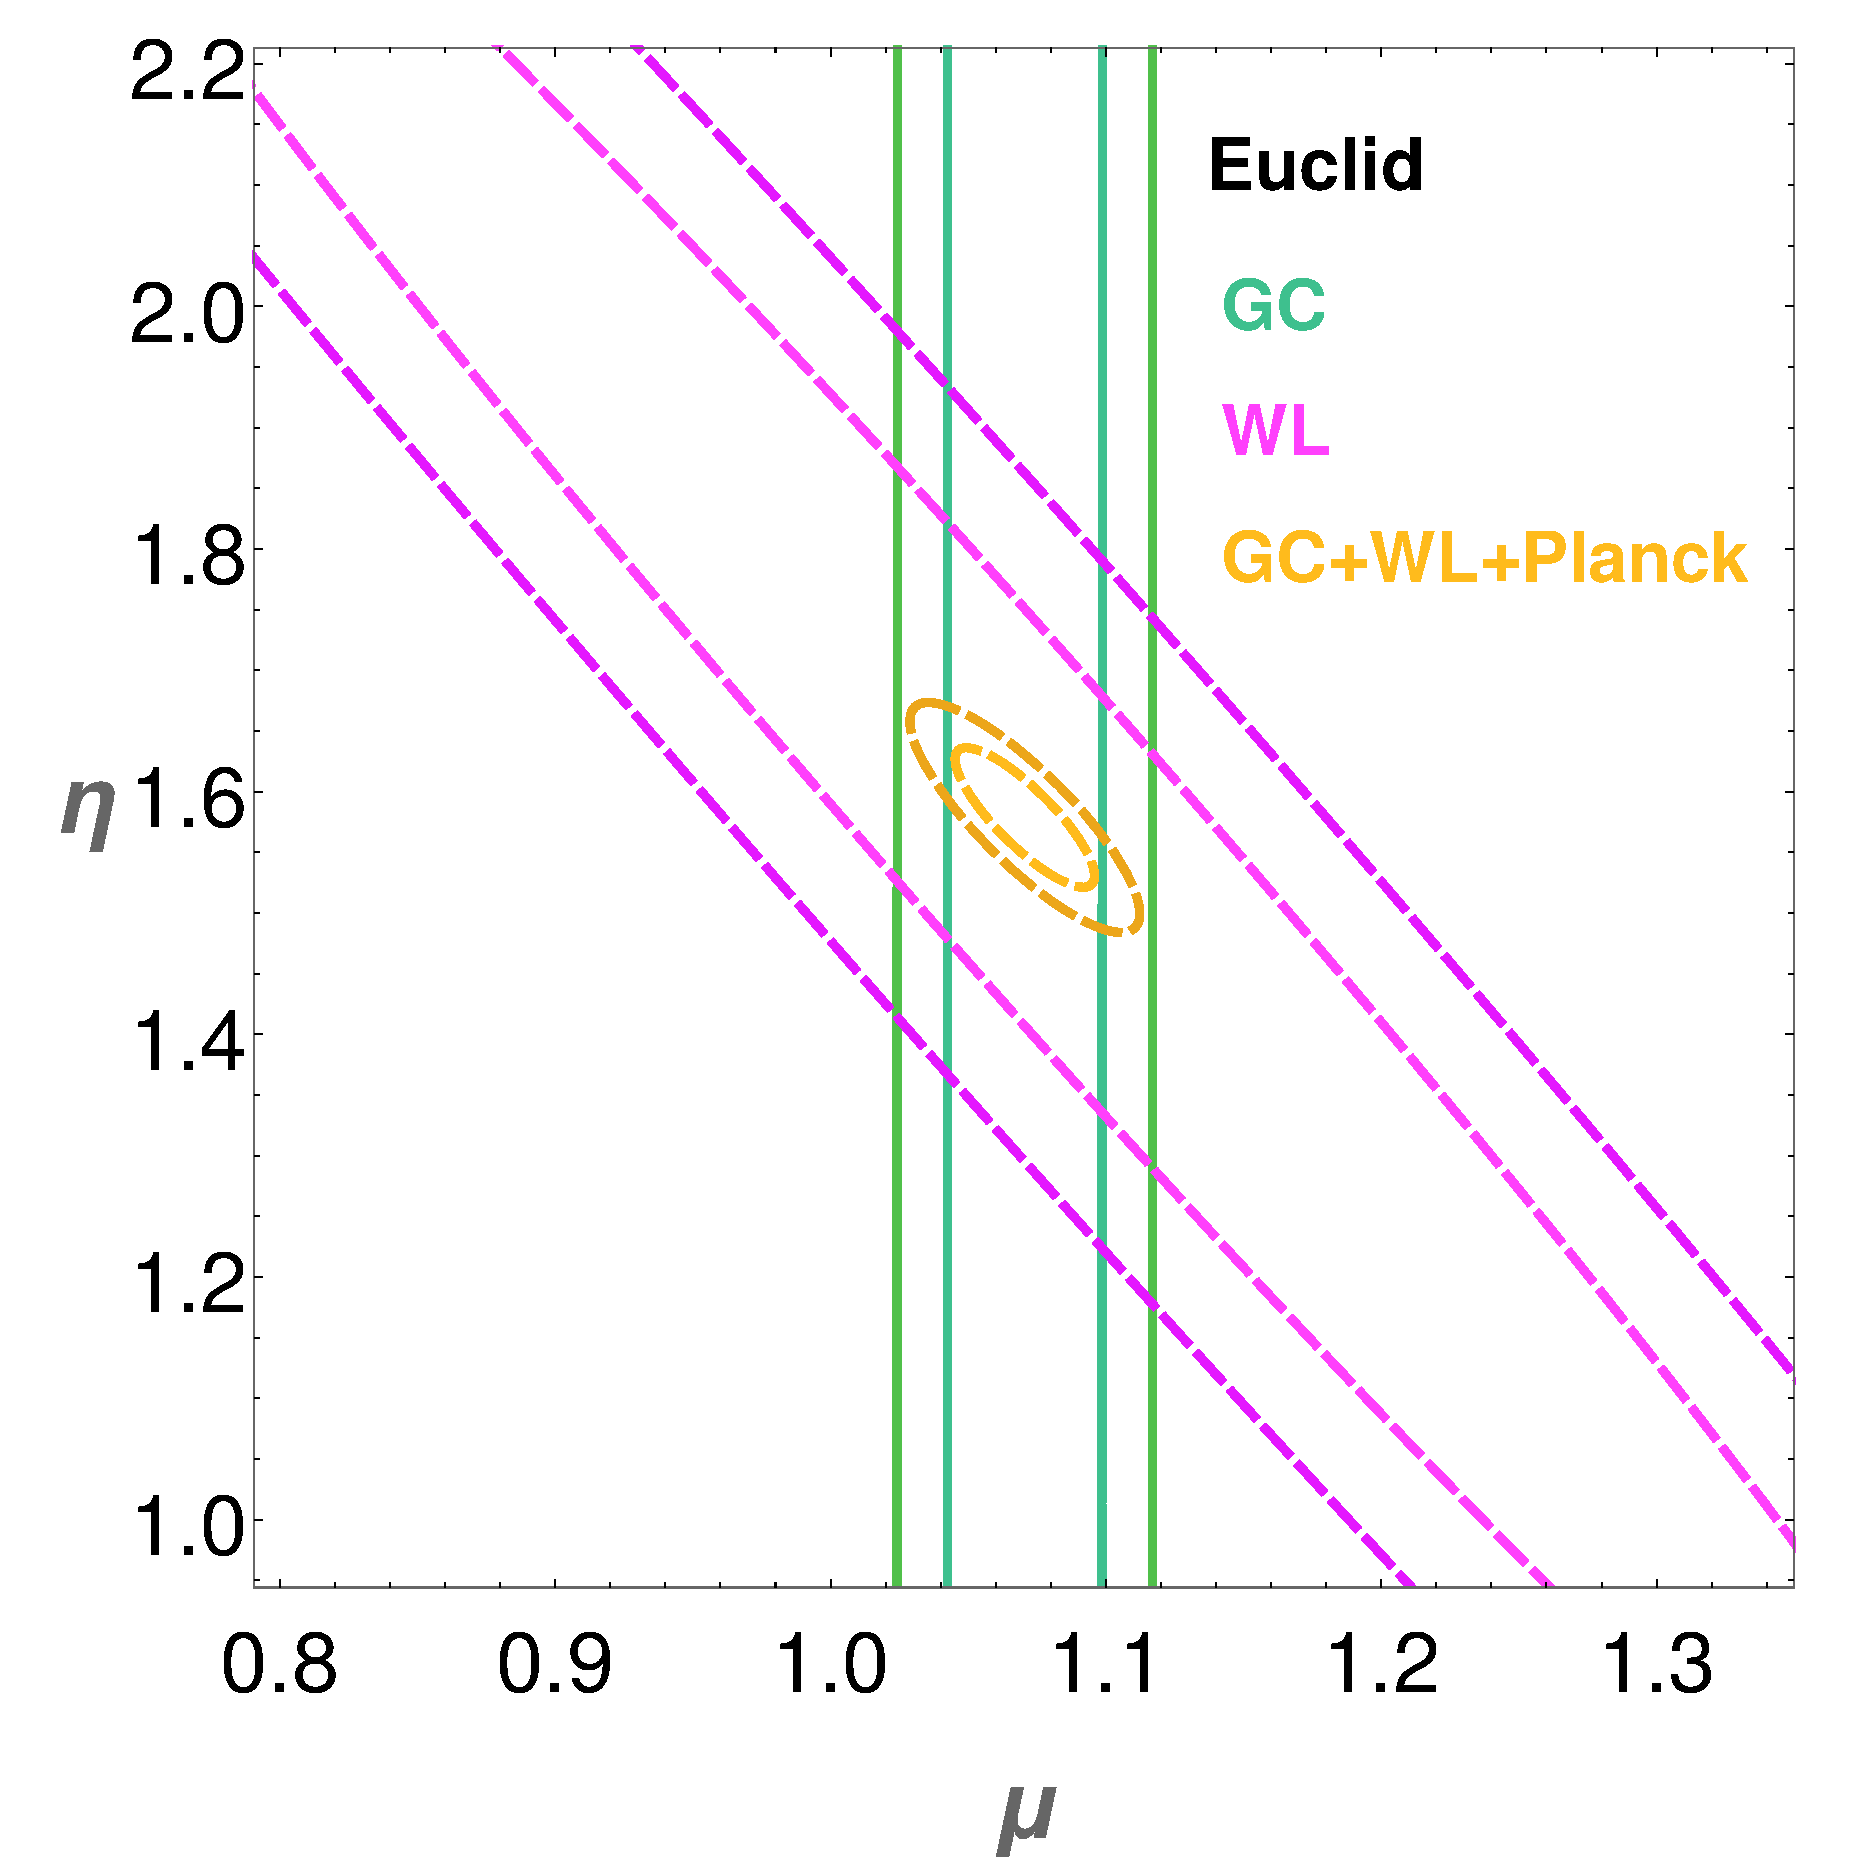
\includegraphics[width=0.45\textwidth]{Chapters/linear-nonlinear-MG-forecasts/figures/ellipses/DE-related/ellipsesPlot-withLegendManual-MuEtaFisher-Marged-fiducialMGDE2nonuhs-GC_WL_GC+WL+Planck--nlHS-pars-6-7_-.pdf}
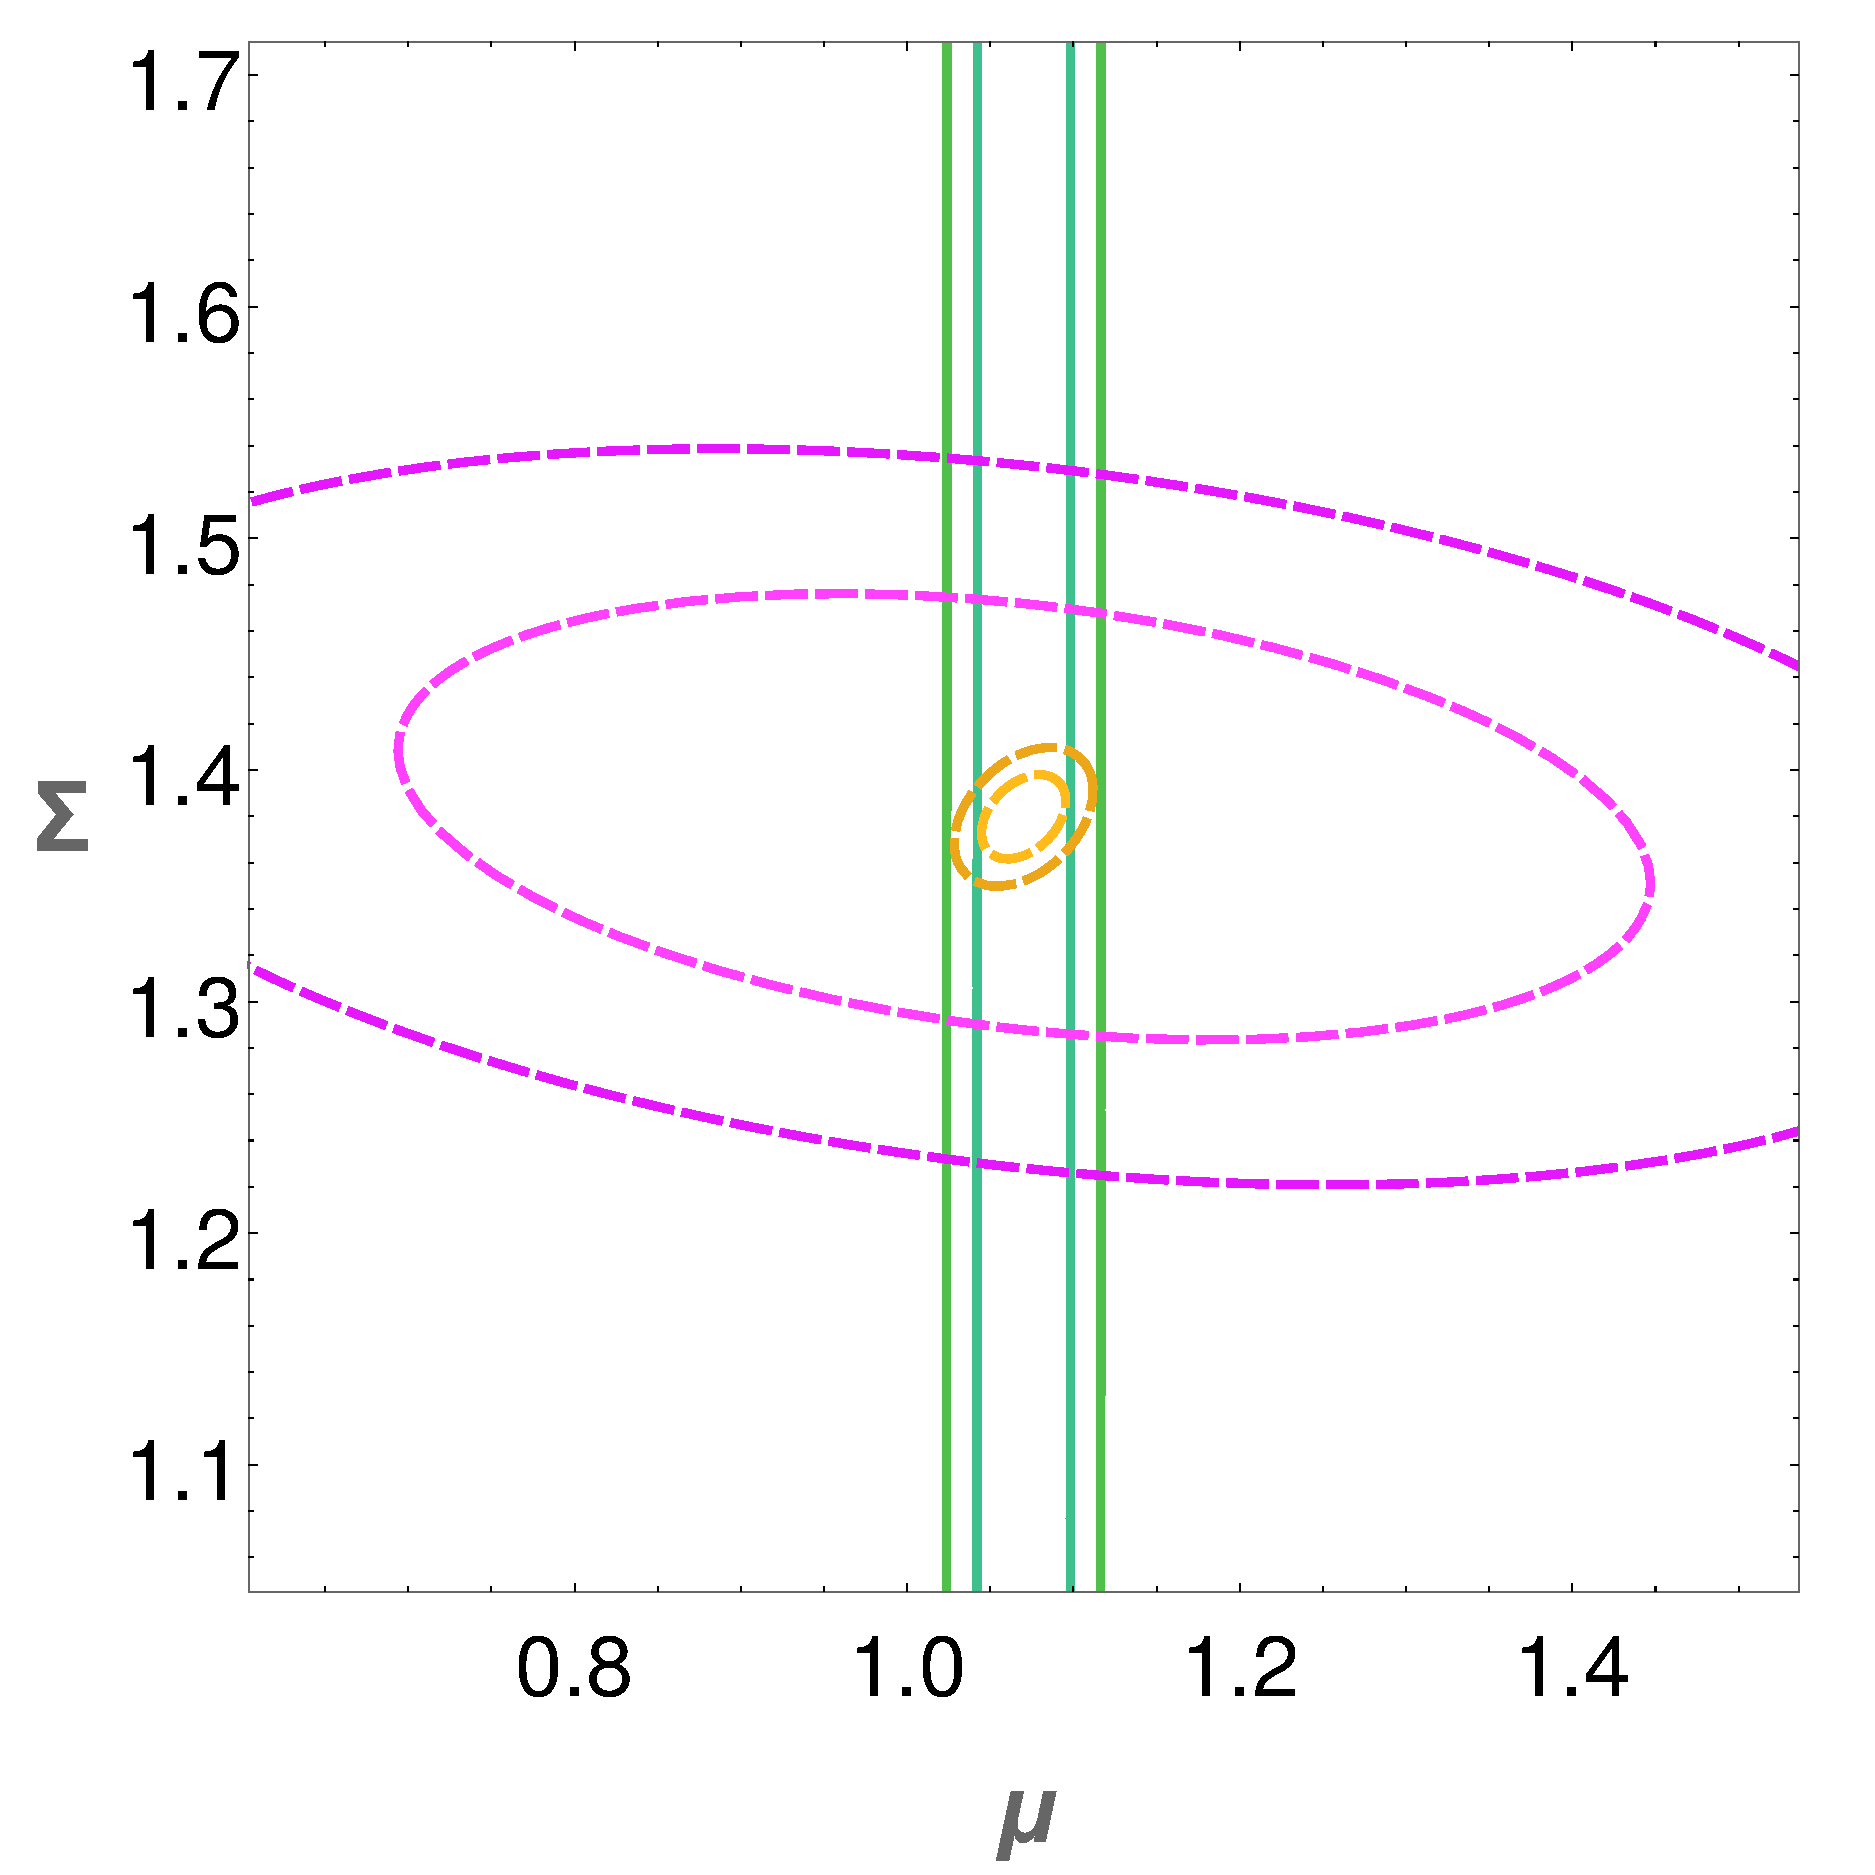
\includegraphics[width=0.45\textwidth]{Chapters/linear-nonlinear-MG-forecasts/figures/ellipses/DE-related/ellipsesPlot-noLegendManual-MuSigmaFisher-Marged-fiducialMGDE2nonuhs-GC_WL_GC+WL+Planck--nlHS-pars-6-7_-.pdf} \\
\end{centering}
\begin{centering}
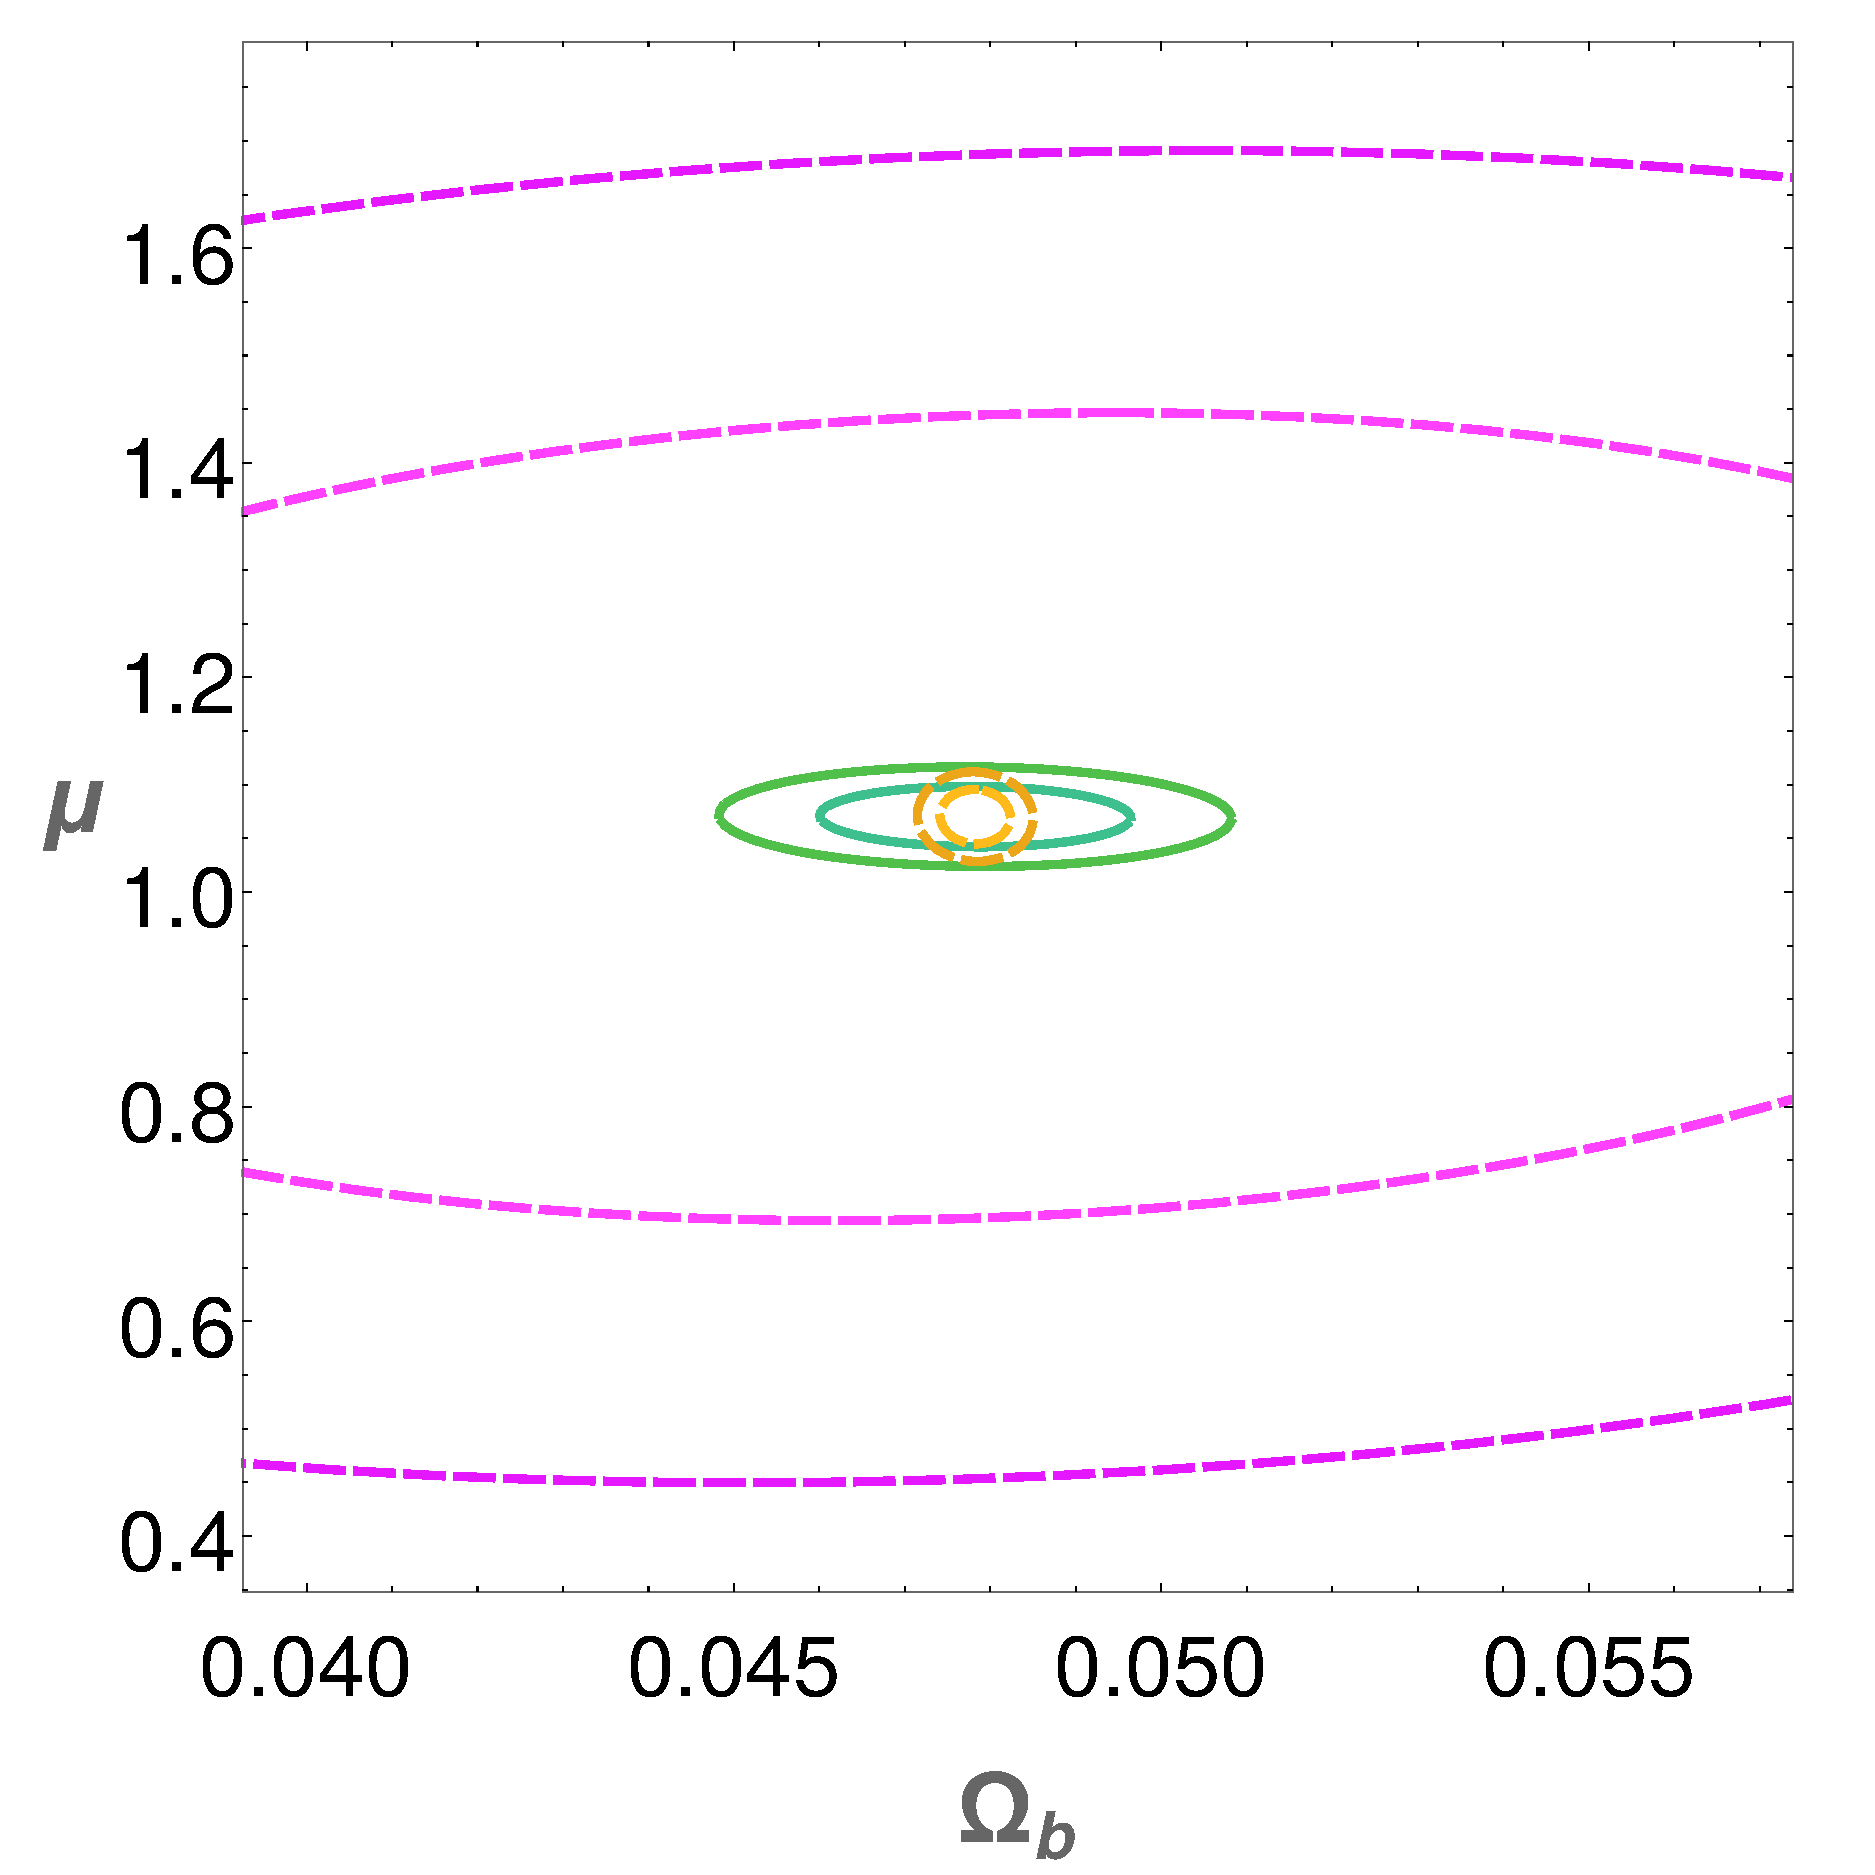
\includegraphics[width=0.45\textwidth]{Chapters/linear-nonlinear-MG-forecasts/figures/ellipses/DE-related/ellipsesPlot-noLegendManual-MuSigmaFisher-Marged-fiducialMGDE2nonuhs-GC_WL_GC+WL+Planck--nlHS-pars-2-6_-.pdf}
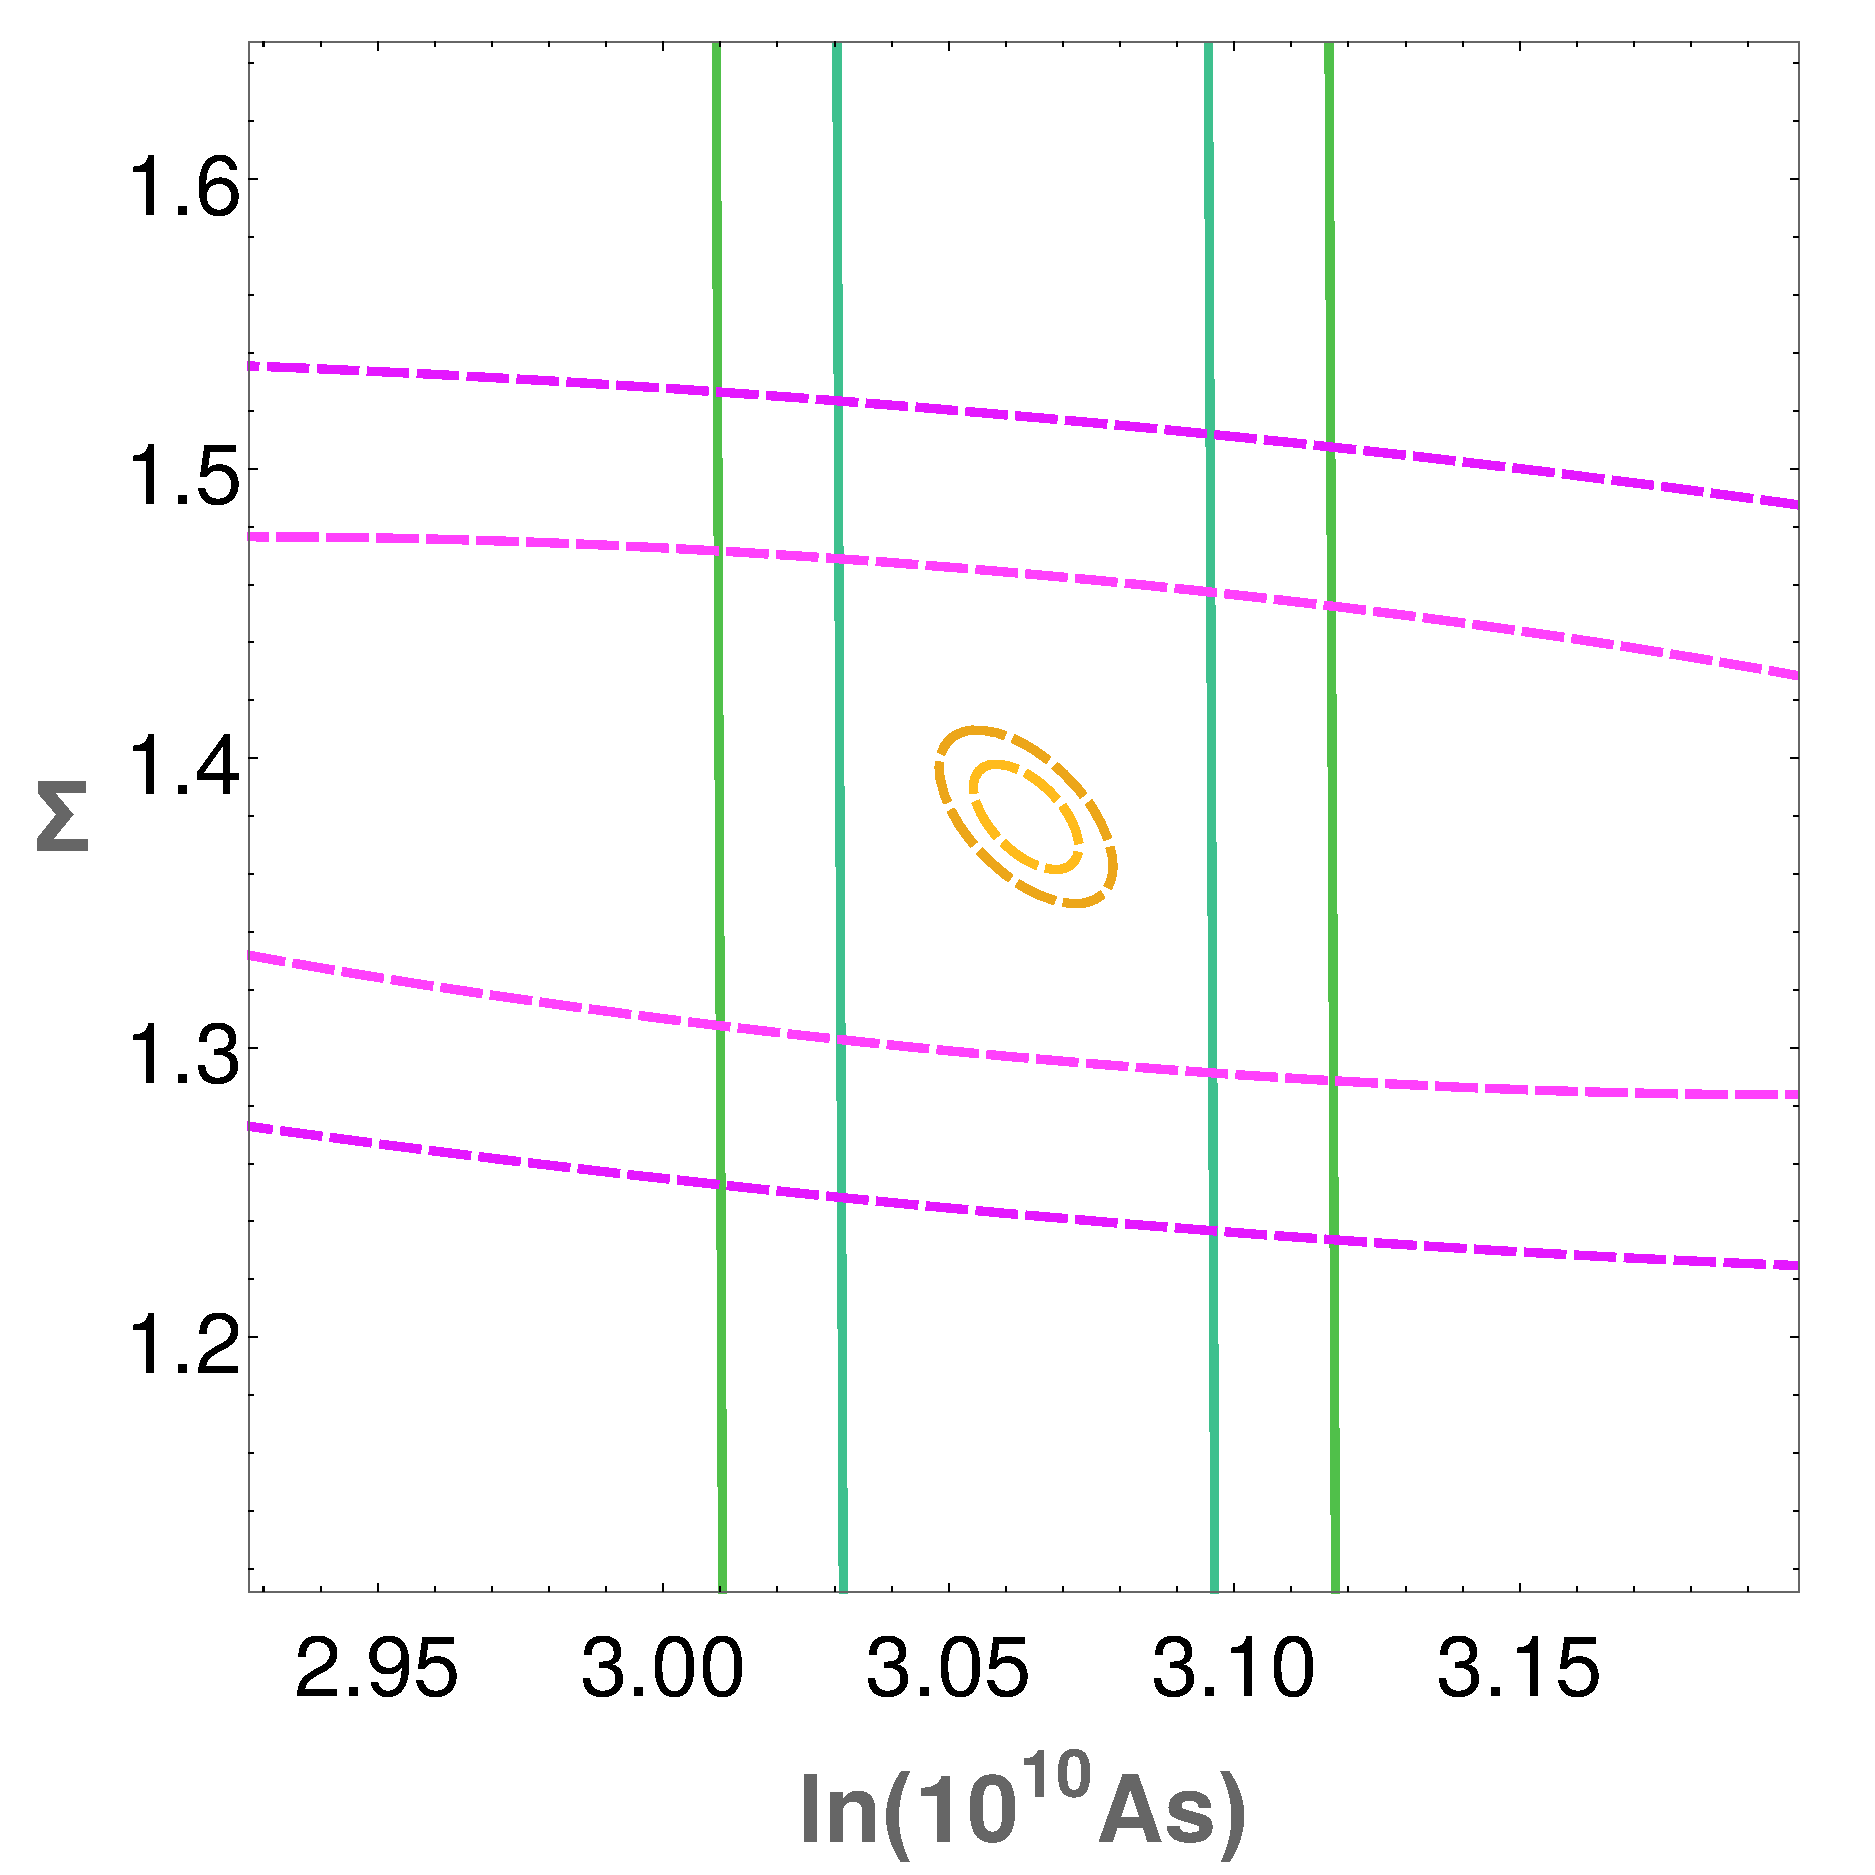
\includegraphics[width=0.45\textwidth]{Chapters/linear-nonlinear-MG-forecasts/figures/ellipses/DE-related/ellipsesPlot-noLegendManual-MuSigmaFisher-Marged-fiducialMGDE2nonuhs-GC_WL_GC+WL+Planck--nlHS-pars-4-7_-.pdf} 
\end{centering}
\caption[Fisher confidence contours for a Euclid GC and WL forecast.]{\label{fig:DE+Planck-ellipses-mu-sig-eta} 
Fisher Matrix marginalized contours
(1, 2 $\sigma$) for the Euclid space mission in the late-time parameterization
using mildly non-linear scales and the HS prescription. Green lines
represent constraints from a Galaxy Clustering survey, pink lines
stand for the Weak Lensing observables, and orange lines represent the GC+WL+{\it Planck} combined confidence
regions. \textbf{Upper Left: }contours for the fully marginalized
errors on $\eta$ and $\mu$. \textbf{Upper Right: }contours for the
fully marginalized errors on $\Sigma$ and $\mu$.\textbf{ Lower Left:
}contours for the fully marginalized errors on $\mu$ and $\Omega_{b}$.
\textbf{Lower Right: }contours for the fully marginalized errors on
$\Sigma$ and $\ln(10^10 A_{s})$. The fact that the combination of GC, WL and \planck\
breaks many degeneracies in the 7-dimensional parameter space, explains why
the combined contours (yellow) have a much smaller area. Notice that in this parametrization, 
GC measures mostly $\mu$ and WL constrains mostly just $\Sigma$.}
\end{figure}

After using the two primary probes from Euclid
separately, we discuss here the constraints obtained combining Weak
Lensing and Galaxy Clustering. 
The combination between GC and
WL can be seen in the bottom panel of Table
\ref{tab:errors-Euclid-GC-WL-late_time}.
In the late-time parameterization, in the linear case, Weak Lensing combined with a galaxy
clustering for a Euclid survey (Redbook specifications) constrains the standard $\Lambda$CDM parameters
in the range $2 \% - 6 \%$, and below 1$\%$ when \planck\ priors are included. Modified Gravity parameters $\mu$ and $\eta$ are now also constrained below 10$\%$, reaching $1\%$ when adding non-linear scales.
The remarkable improvement can be attributed
to the fact that the combination of GC and WL Fisher matrices breaks
many degeneracies in the parameter space. This is shown in Figure
\ref{fig:DE+Planck-ellipses-mu-sig-eta}, where it is possible to notice
how the two probes are almost orthogonal both in the $\mu$-$\eta$-
and $\mu$-$\Sigma$-plane. Weak Lensing measures
the changes in the Weyl potential, parametrized by $\Sigma$, while $\mu$ is related to the Poisson equation, and therefore to the potential $\Psi$, modified by peculiar velocities and sensitive to Galaxy Clustering; $\eta$ can also be written as a combination of $\mu$ and $\Sigma$ (see Eqn.\ \ref{eq:SigmaofMuEta}). 

Further improvement is brought by the sensitivity of Galaxy Clustering to standard $\Lambda$CDM parameters; even
though GC constraints on $\Sigma$ and $\eta$ are not as good as the ones for Weak Lensing, the better measurement of standard parameters provided by Galaxy Clustering breaks degeneracies in the Modified Gravity sector of the parameter space, leading to
narrower bounds for $\eta$ and $\Sigma$ with respect to both probes taken separately. WL is instead not sensitive to modifications of the Poisson equation for matter and this explains why constraints on $\mu$ are not improved
by the combination of the two probes, but are rather dominated by
GC. 
The correlation among parameters can also help us explain the observed results. 
The Figure of Correlation, defined in Eq.\ (\ref{eq:FoC}), for GC (non-linear HS) alone is 4.9, while
for WL (non-linear HS) the correlation is higher, with $\textrm{FoC}=16.9$.
When combining both probes (GC+WL (non-linear HS)) the FoC goes to an intermediate point of 7.6.

Given the constraining power of the GC+WL combination on MG functions, adding the \planck\ priors does not lead to significant improvements on the dark energy related parameters. On the other hand, standard parameters significantly benefit
from the inclusion of CMB and background priors and we can expect
this to be a relevant factor for MG models with degeneracies
with $\Lambda$CDM parameters, e.g. models affecting also the expansion
history of the universe.
An overview of the constraints on Modified Gravity described in this section is shown in Fig.\ref{fig:DE+Planck-ellipses-mu-sig-eta}, with Euclid GC, Euclid WL and Euclid GC+WL combined with \planck\ priors.


\subsubsection{Derivatives of the Power Spectrum with respect to $\mu$ and $\eta$}\label{sec:appder}

In this section we investigate the derivatives of the power spectrum with respect to the MG parameters. 
Using the Jacobians from \cref{subsub:Jacobian}, we can convert 
our fundamental derivatives $\partial P(k,z)/\partial E_{ij}$ to derivatives of $\partial P(k,z)/\partial (\mu, \eta)$ evaluated at $z=0$.

\begin{figure}[htbp]
	\centering{}
	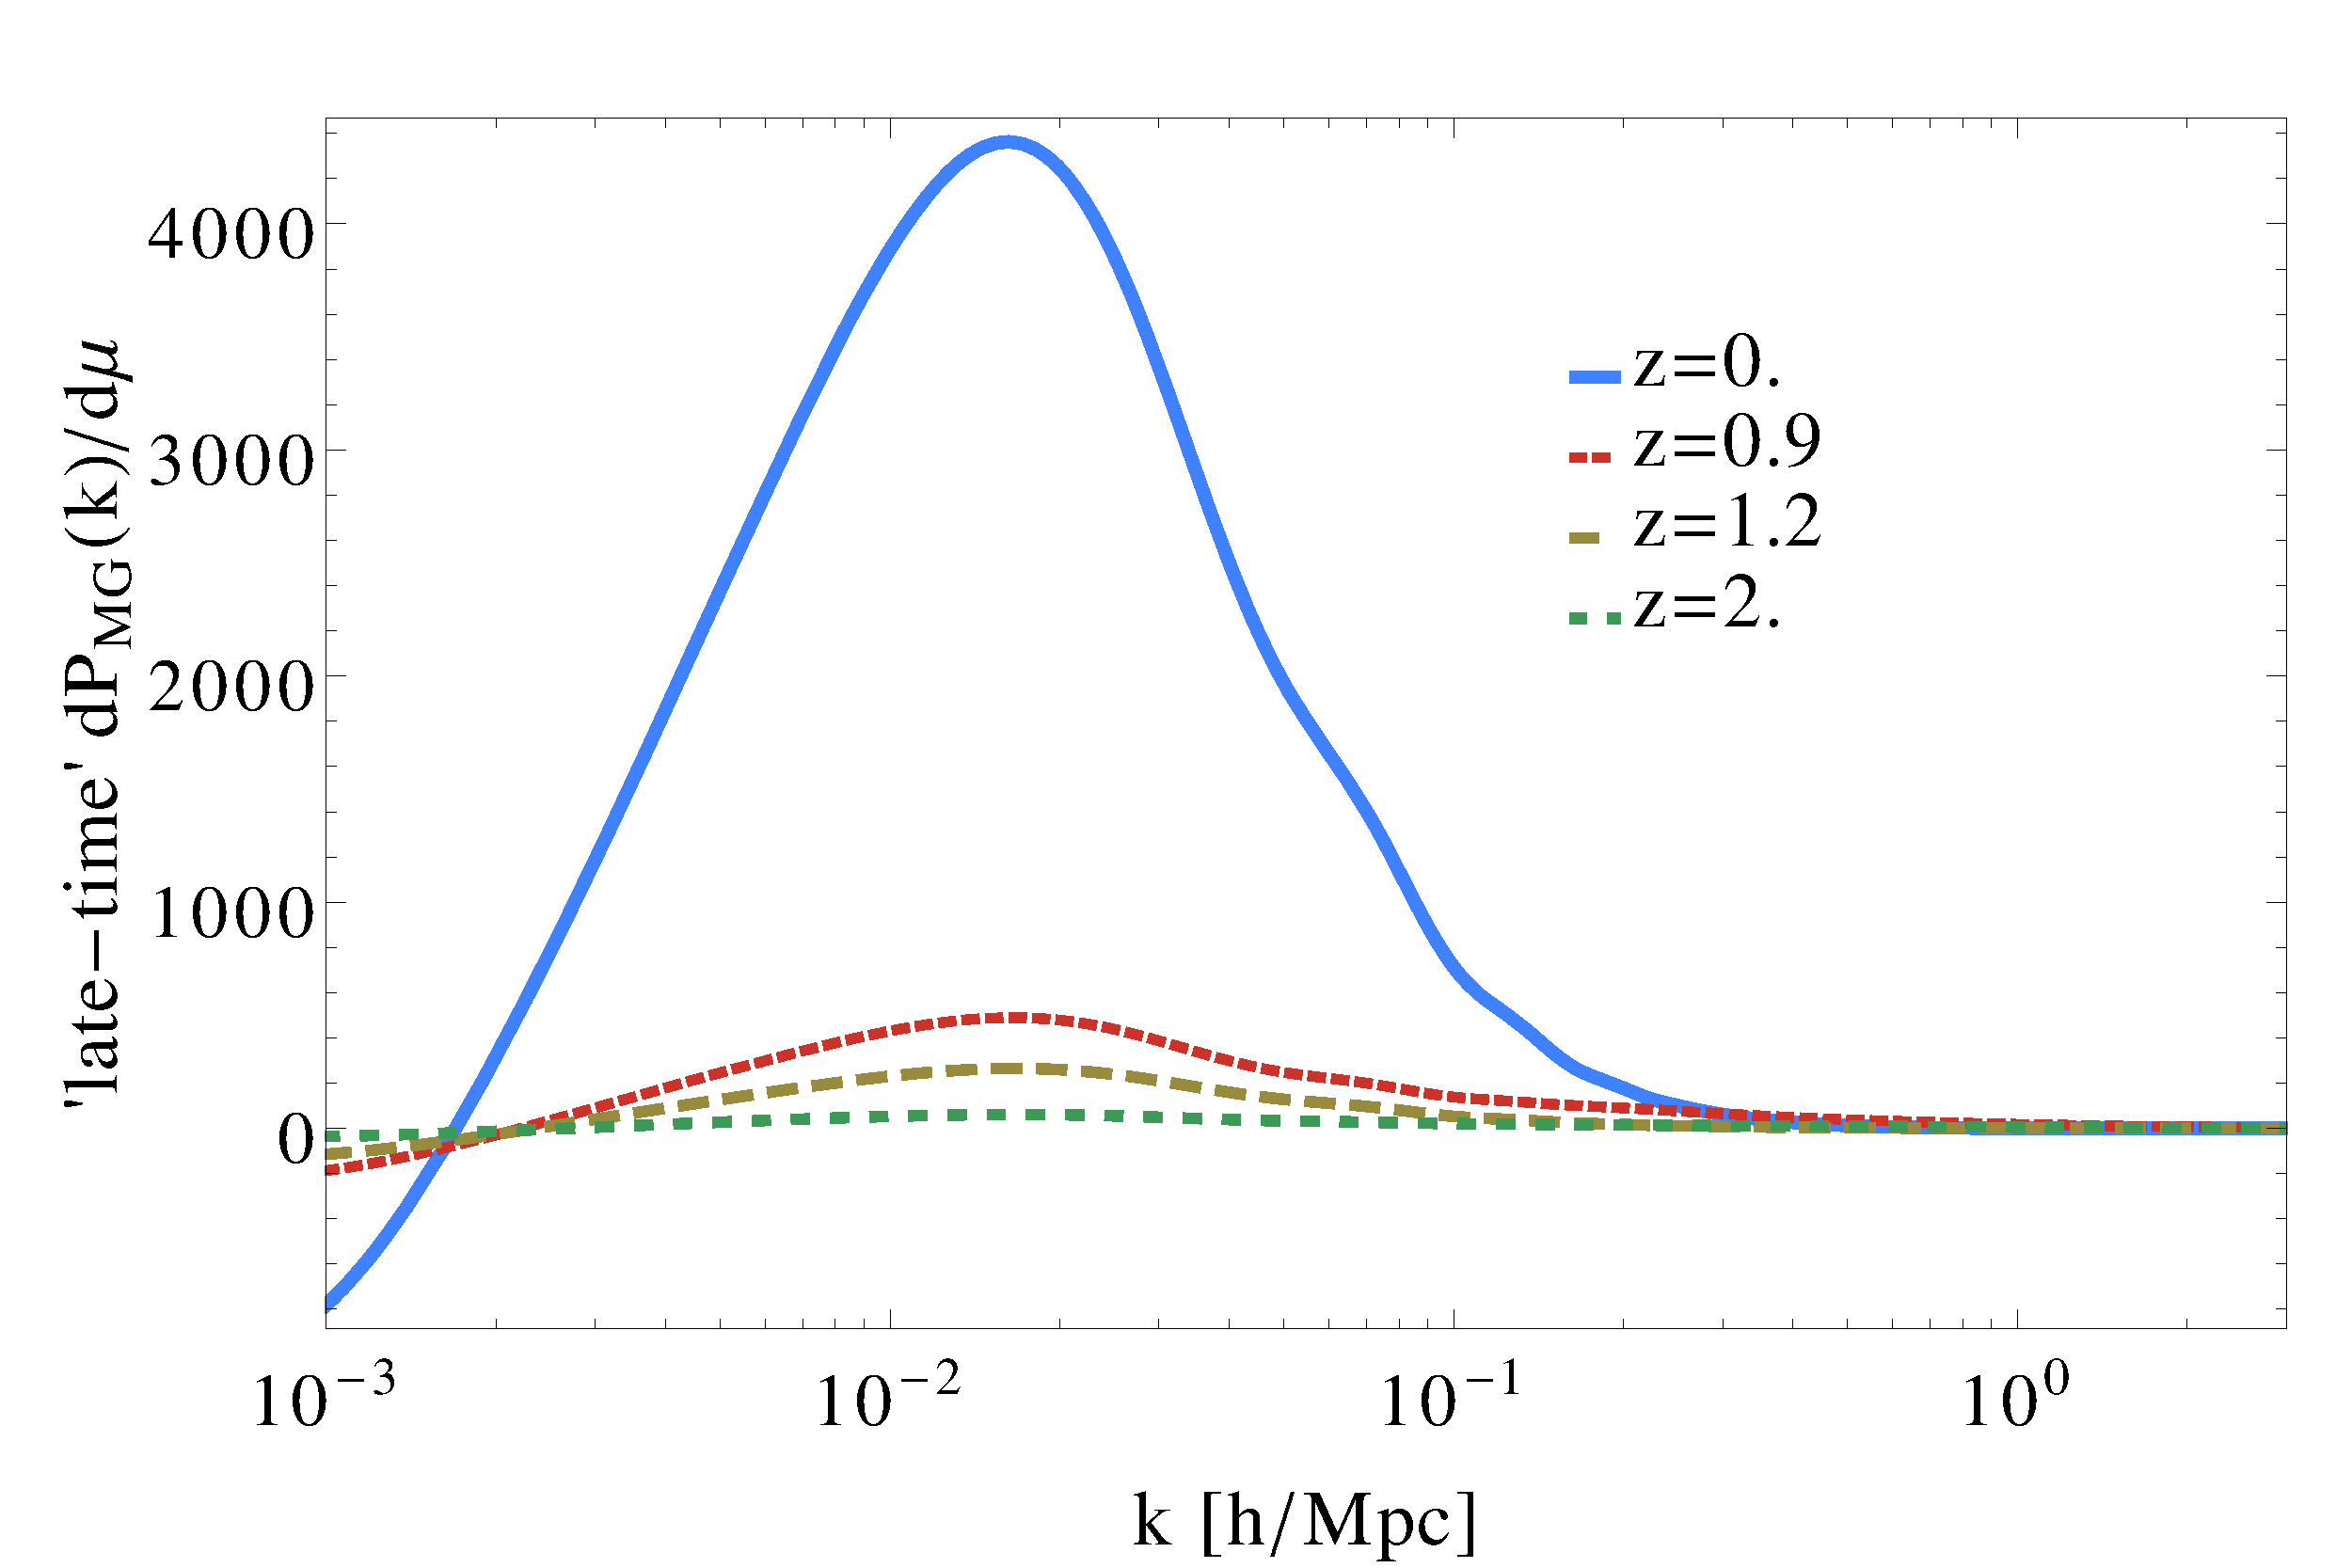
\includegraphics[width=0.4\textwidth]{Chapters/linear-nonlinear-MG-forecasts/figures/power-spectra/derivs/MGDE-Pk-wrt-mu-4z.pdf}
	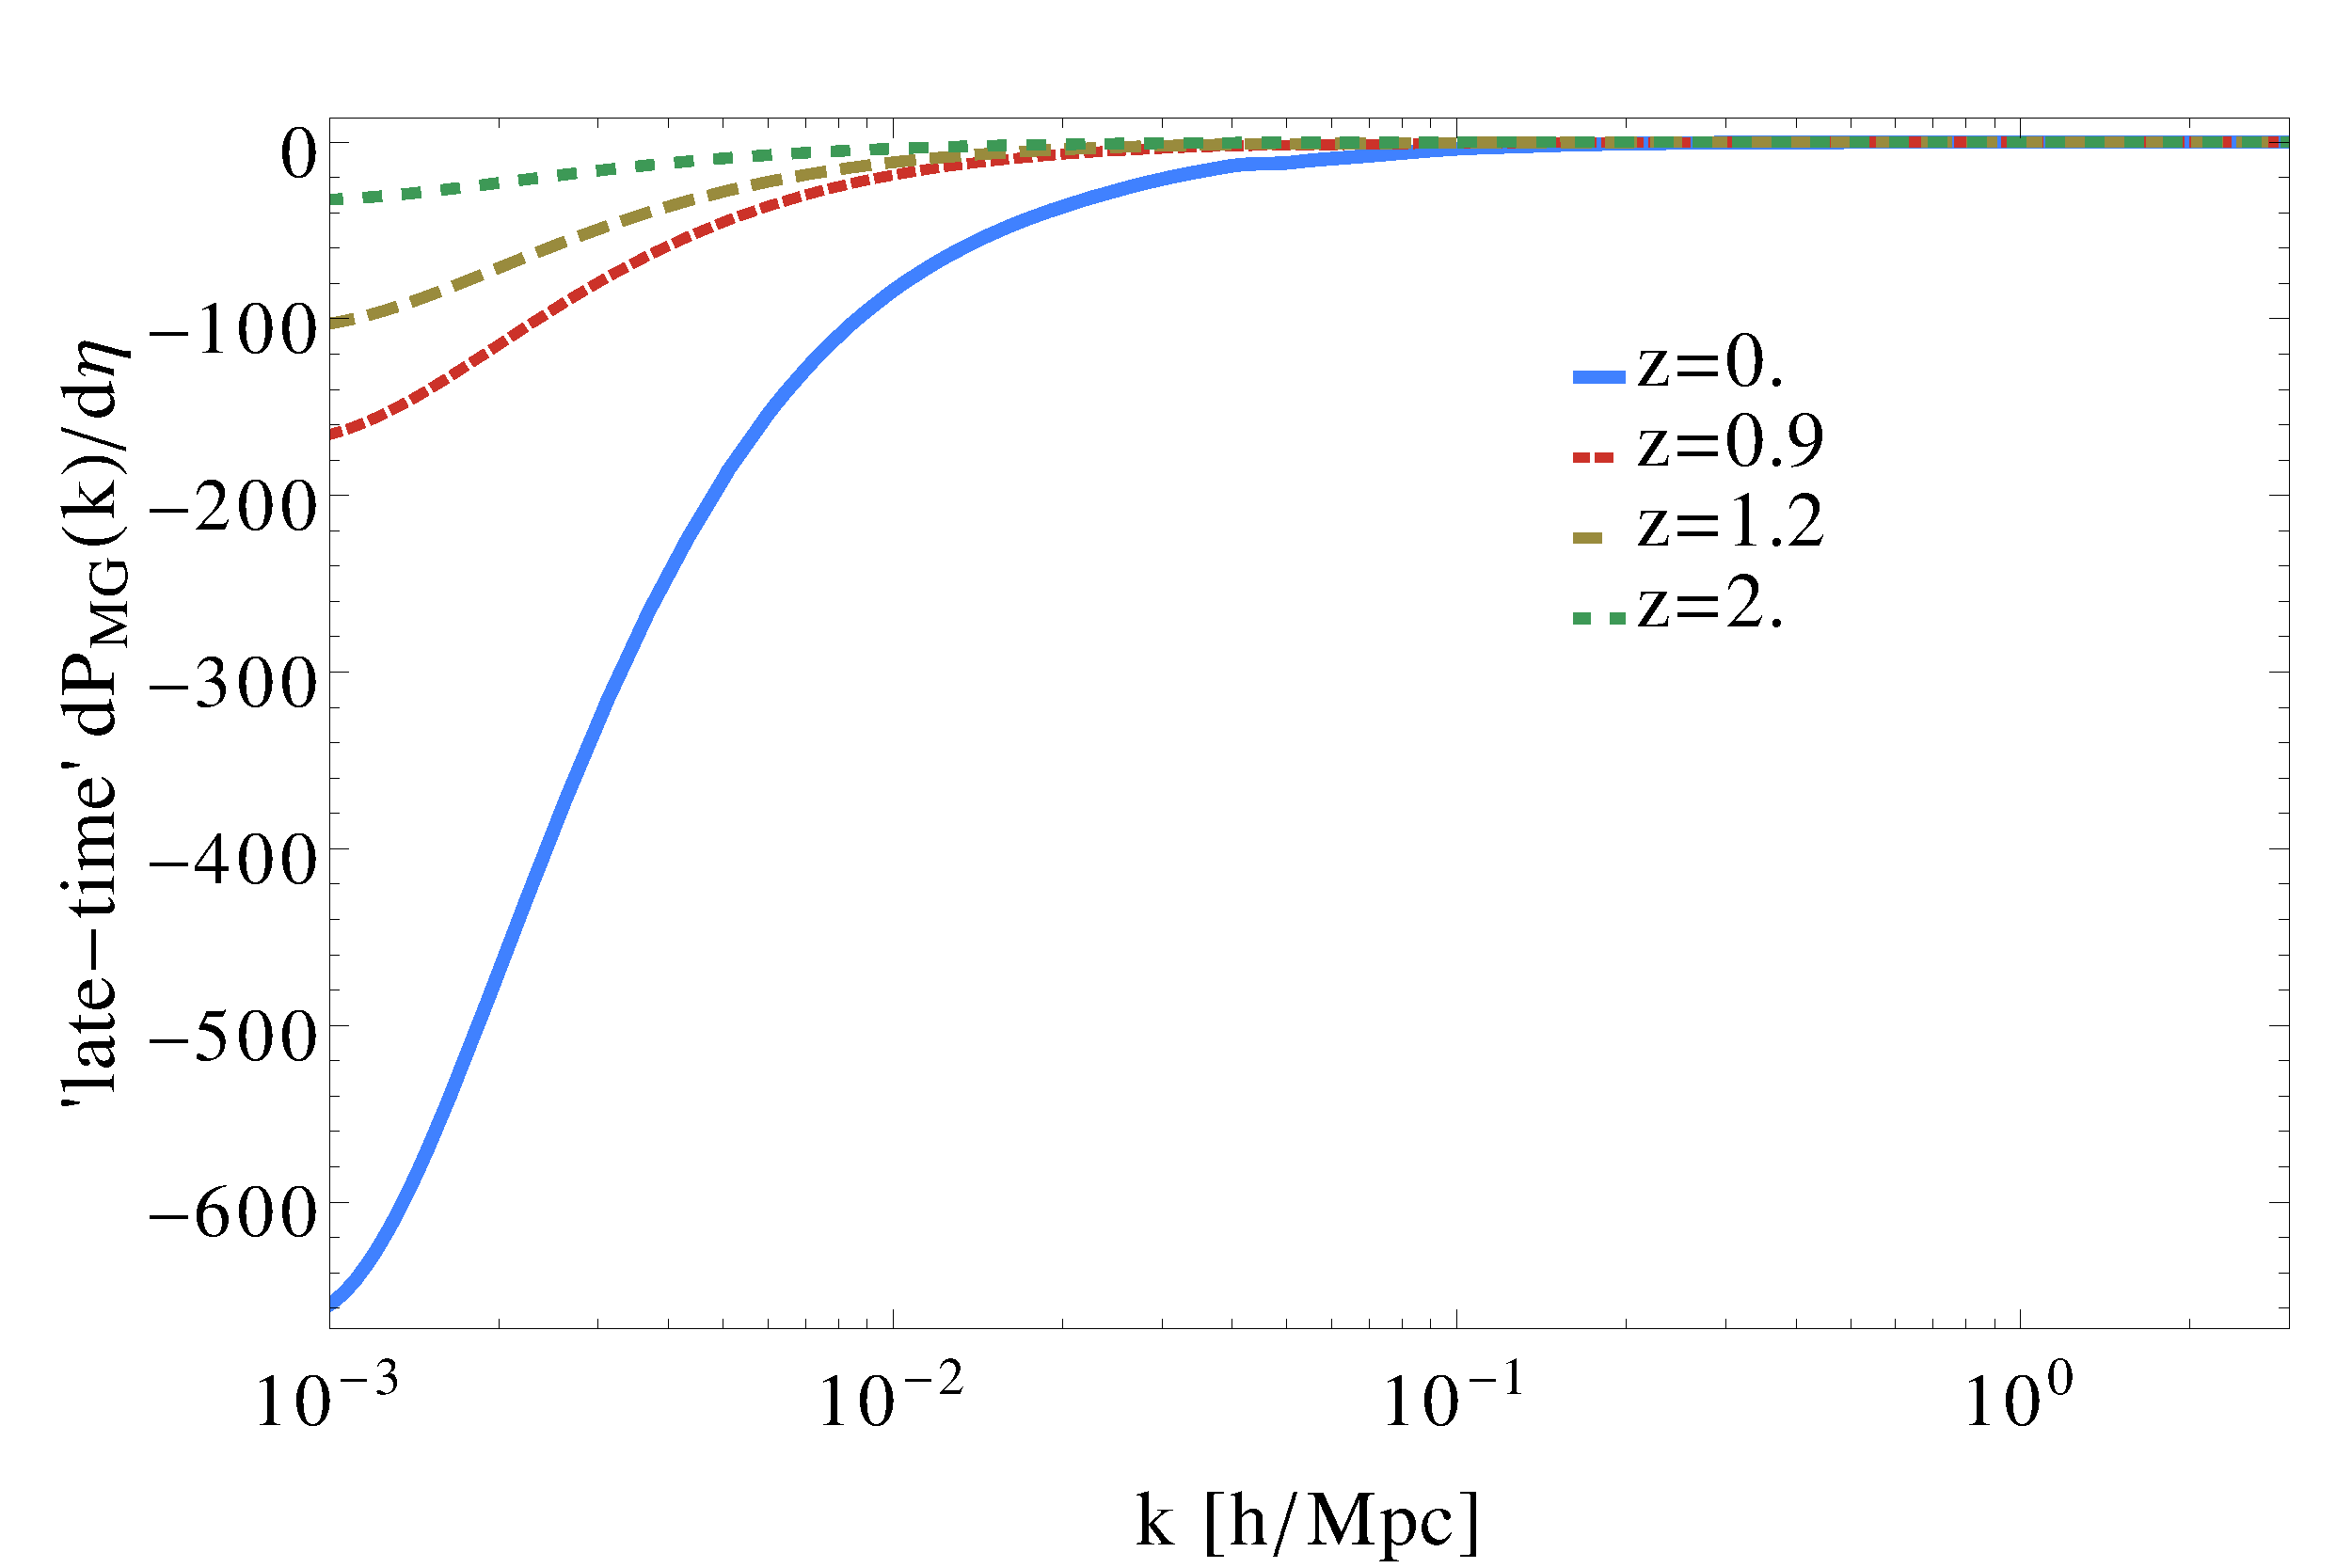
\includegraphics[width=0.4\textwidth]{Chapters/linear-nonlinear-MG-forecasts/figures/power-spectra/derivs/MGDE-Pk-wrt-eta-4z.pdf}
	\caption[Derivatives of the power spectrum in the late-time parameterization.]{ Derivatives of the matter power spectrum $P(k,z)$ w.r.t. the MG parameters $\mu$ and $\eta$ in the late-time parametrization.
	}\label{fig:Pkderivs-latetime}
\end{figure}


\begin{figure}[htbp]
	\centering{}
	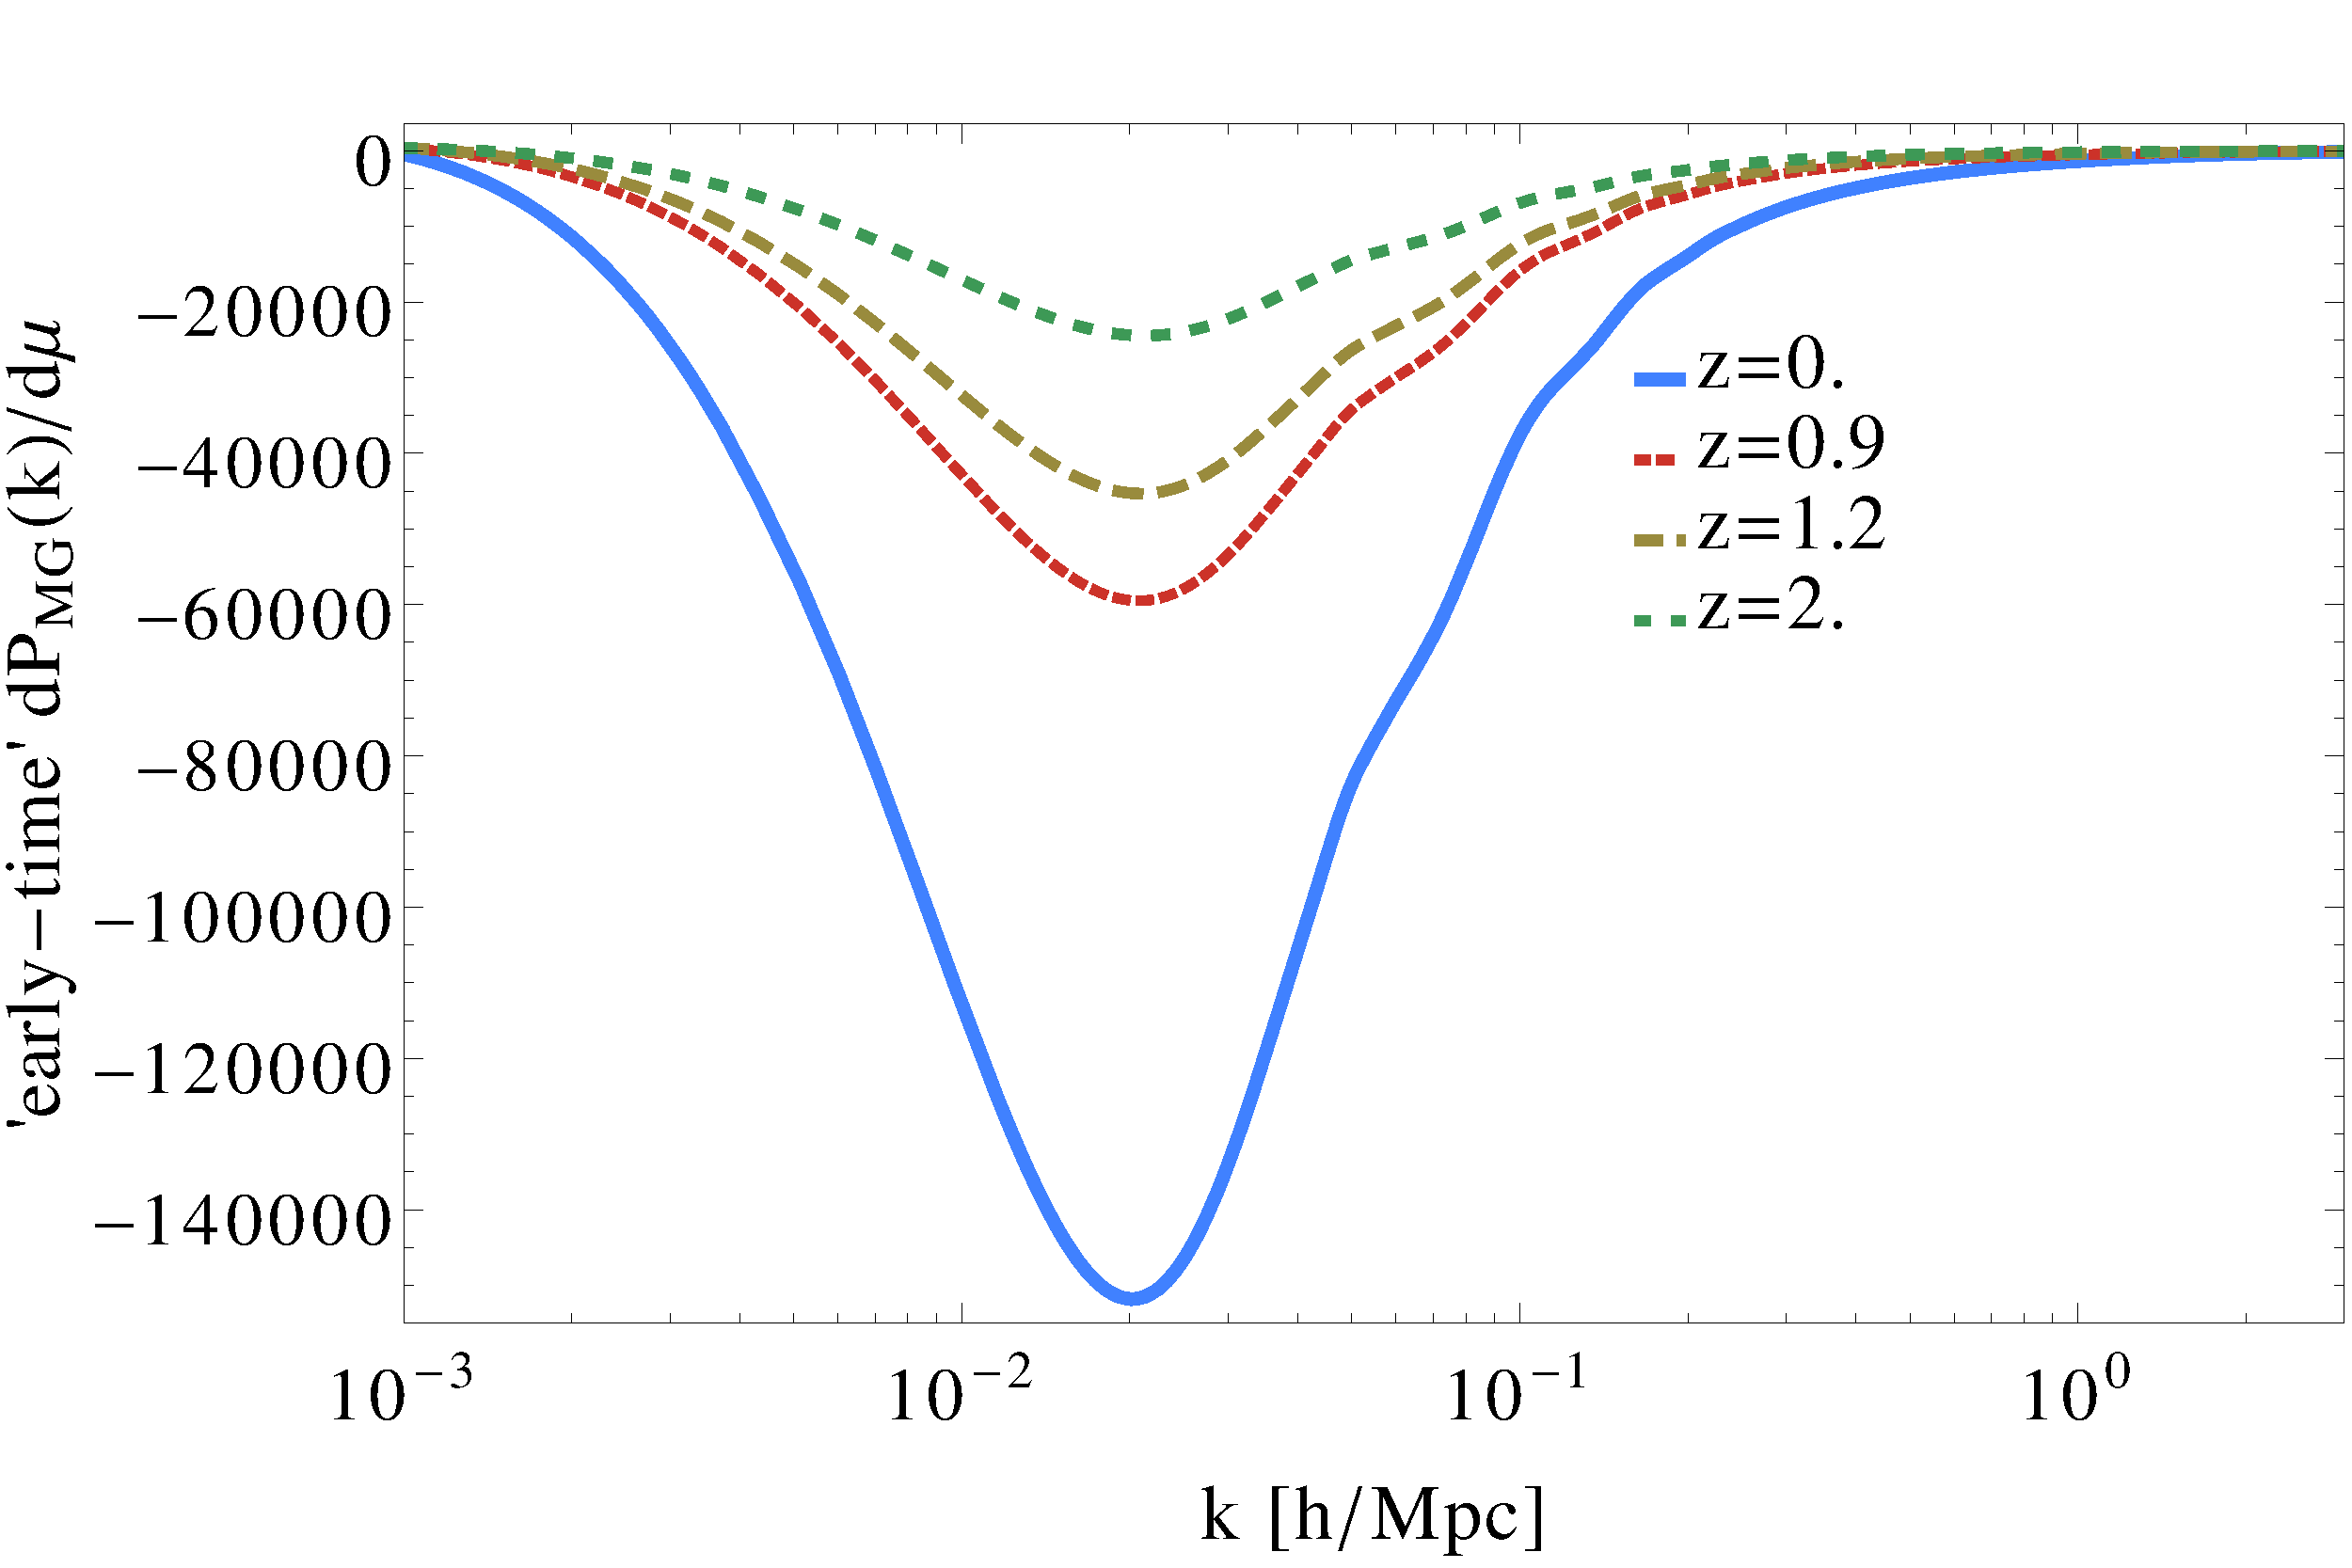
\includegraphics[width=0.4\textwidth]{Chapters/linear-nonlinear-MG-forecasts/figures/power-spectra/derivs/MGTR-Pk-wrt-mu-4z.pdf}
	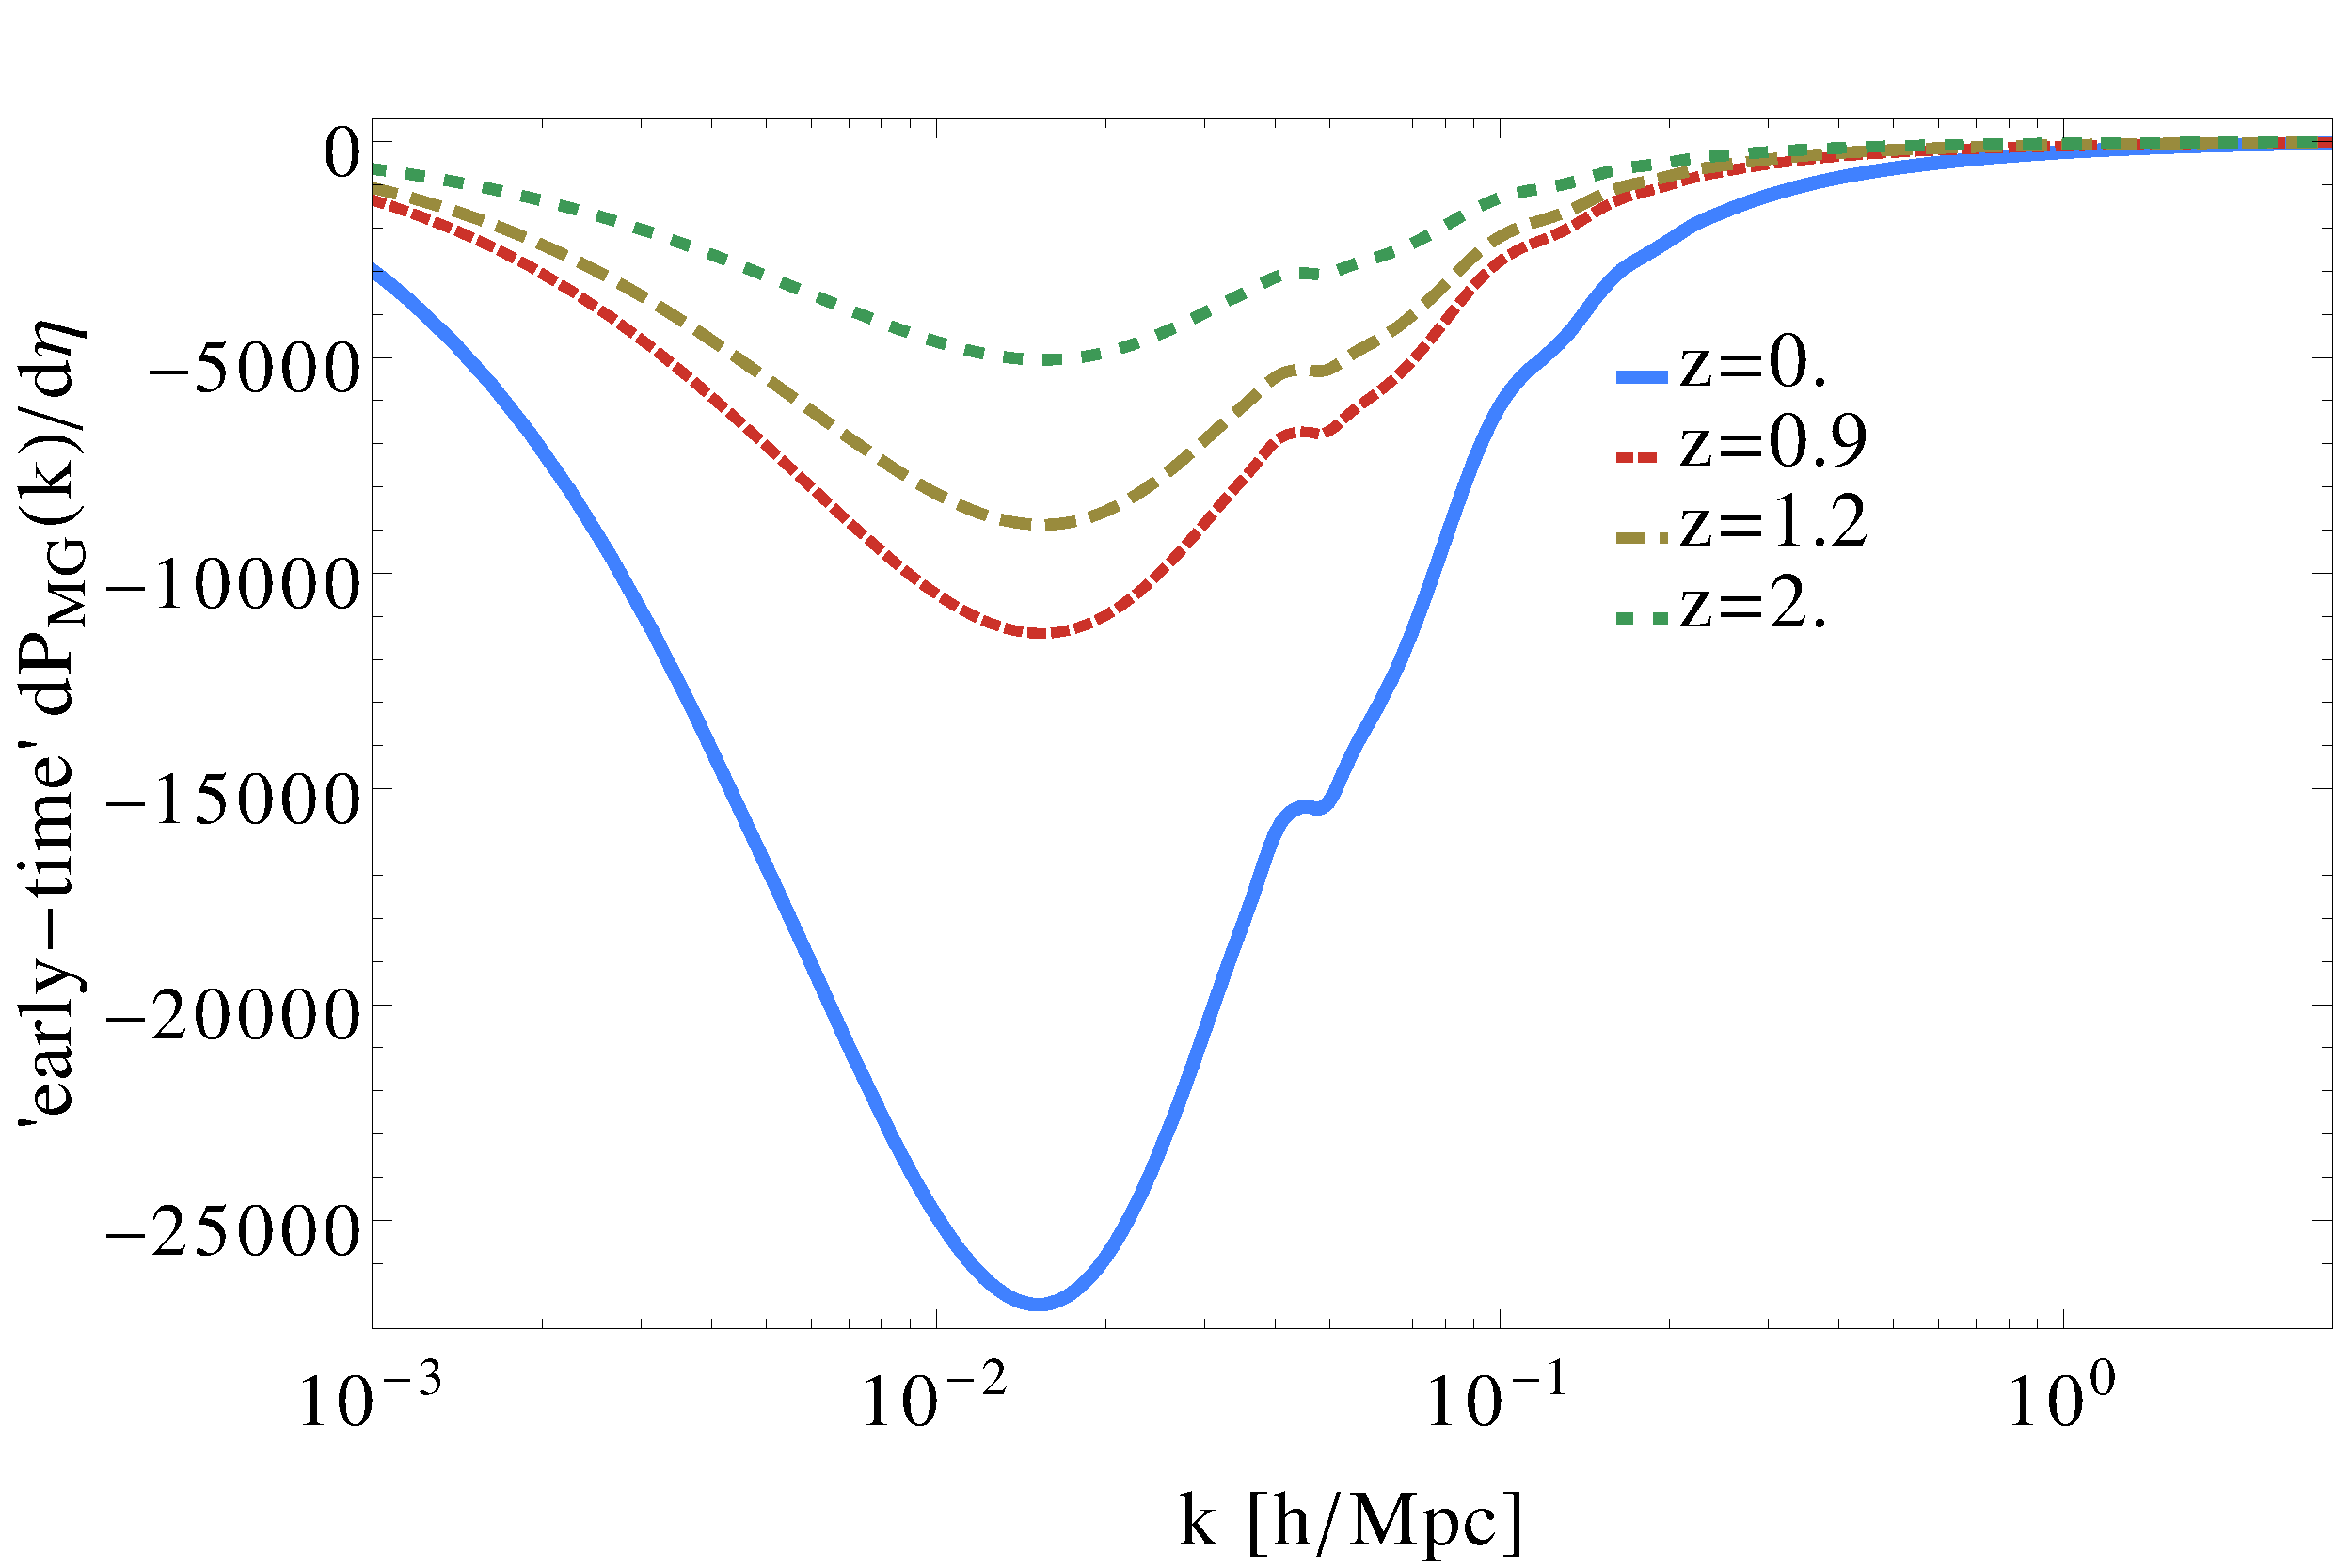
\includegraphics[width=0.4\textwidth]{Chapters/linear-nonlinear-MG-forecasts/figures/power-spectra/derivs/MGTR-Pk-wrt-eta-4z.pdf}
	\caption[Derivatives of the power spectrum in the early-time parameterization.]
	{ Derivatives of the matter power spectrum $P(k,z)$ w.r.t. the MG parameters $\mu$ and $\eta$ in the early-time parametrization.
	}\label{fig:Pkderivs-latetime}
\end{figure}

We can see from the previous figures that in the early-time parametrization the derivative of the power spectrum
with respect to $\eta$ has a similar shape as the derivative with respect to $\mu$, making $\eta$ detectable by a Galaxy Clustering survey.
To explain this, we derive the equation governing the evolution of density fluctuations for a cold dark matter (CDM) species, based on the equations
implemented on the code MGCAMB presented in \cite{hojjati_testing_2011}, expressed here in the conformal Newtonian gauge.
In the following, a dot represents derivative with respect to conformal time $\tau$:
\begin{align}
\dot \delta &= - (1+w)(\theta - 3 \dot \Phi) - 3 \mathcal{H}(\frac{\delta P}{\delta \rho}-w)\delta\\
\dot \theta &= - \curH (1-3w)\theta - \frac{\dot w}{1+w} \theta + \frac{\delta P / \delta \rho}{1+w} k^2 \delta - k^2 \sigma + k^2 \Psi
\end{align}
For CDM we have $\sigma = w = c^2_s= \delta P / \delta \rho  = 0$,  then:
\begin{align}
\dot \delta &= -(\theta - 3 \dot \Phi) \label{eq:deltadot}\\
\dot \theta &= -\curH \theta + k^2 \Psi \label{eq:thetadot}
\end{align}
We have parameterized the solution to $\Psi$ as:
\begin{equation}\label{eq:Psipoisson}
k^2 \Psi = -4 \pi G a^2 \mu(\tau) \rho(\tau) \delta(\tau) \quad ,
\end{equation}
and since we are also requiring gravitational slip $\eta = \Phi / \Psi$, we then have the Poisson equation for $\Phi$:
\begin{equation}
k^2 \Phi = -4 \pi G a^2 \mu(\tau) \eta(\tau) \rho(\tau) \delta(\tau) \label{eq:Phipoisson}
\end{equation}

\done\todo{check alignmenent of figs}
Taking the time derivative of (\ref{eq:deltadot}) and using (\ref{eq:thetadot}) and (\ref{eq:deltadot}) to 
replace $\dot \theta$ and $\theta$, and substituting $\Psi$ from (\ref{eq:Psipoisson}), we obtain:
\begin{align}\label{eq:dotdotdelta-mueta}
\ddot{\delta} + \curH \dot{\delta} &= 3\curH \dot{\Phi} + 3\ddot{\Phi} + 4 \pi G a^2 \mu \rho \delta
\end{align}

In general, derivatives of $\Phi$ appearing on the right hand side will depend on both $\mu$ and $\eta$. Their contribution is larger in the early-time parameterization with respect to the late-time one.


\subsubsection{Forecasts in Modified Gravity for SKA1, SKA2 and DESI \label{subsub: other-surveys-late-time}}

\begin{figure}[htbp]
\begin{centering}
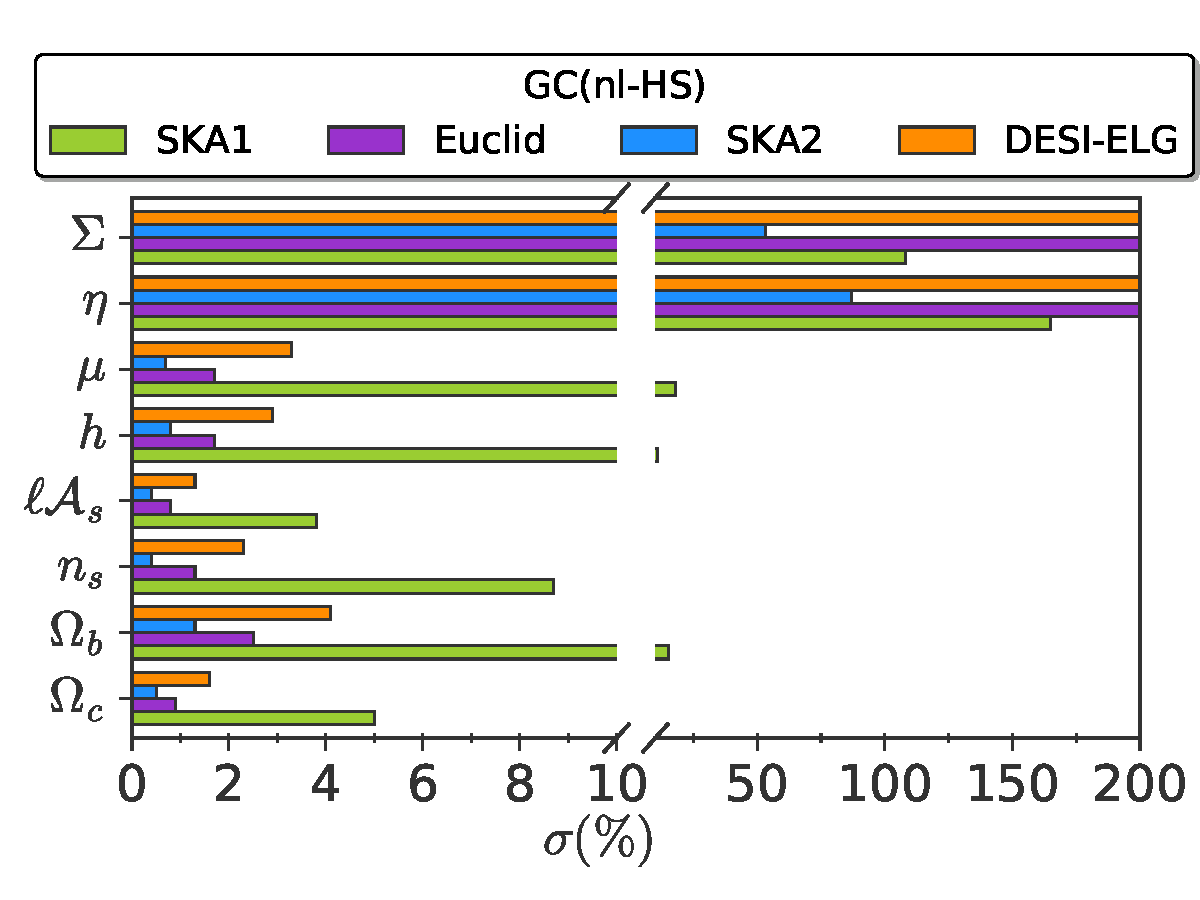
\includegraphics[width=0.45\textwidth]{Chapters/linear-nonlinear-MG-forecasts/figures/BarPlots/4surveys-GCnlHS-MGDE-latetime}\hspace{-0.5pt}
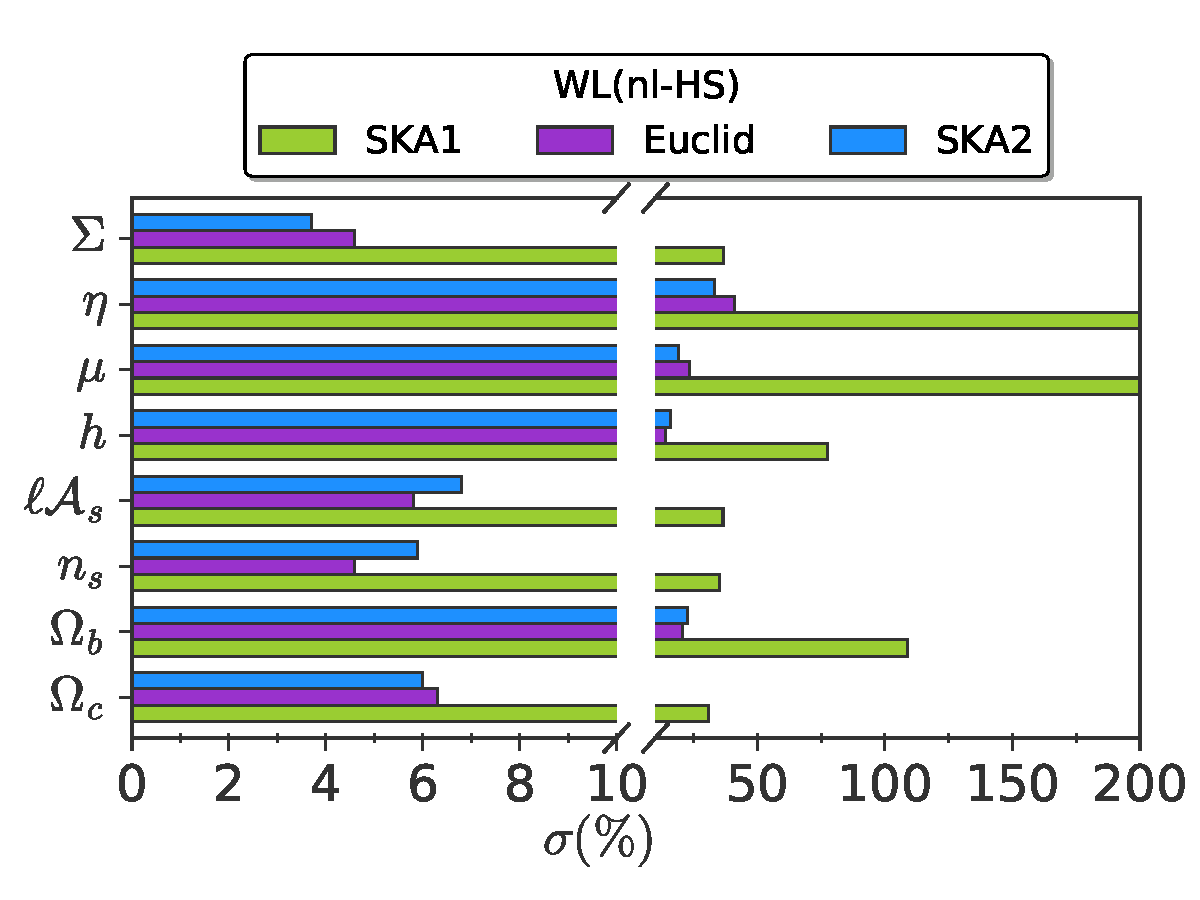
\includegraphics[width=0.45\textwidth]{Chapters/linear-nonlinear-MG-forecasts/figures/BarPlots/4surveys-WLnlHS-MGDE-latetime.pdf}

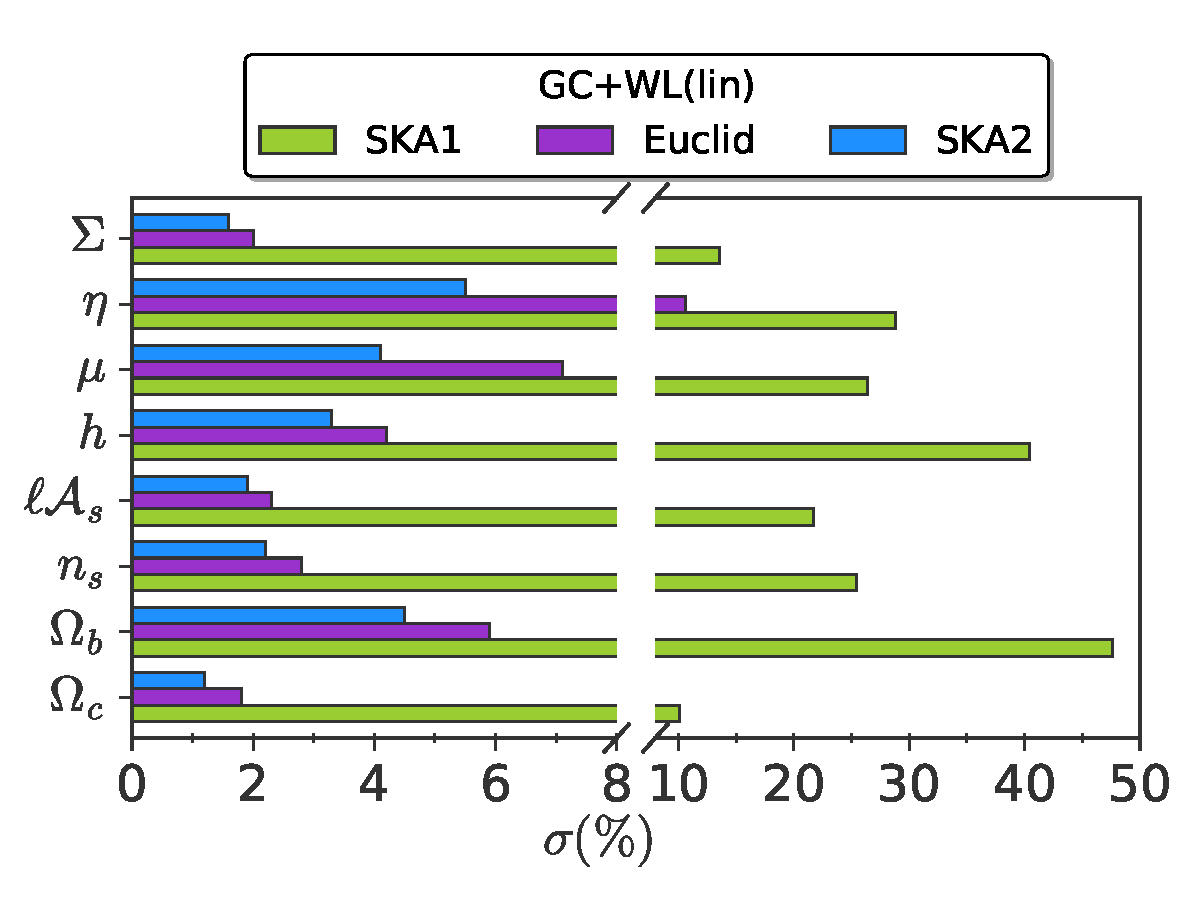
\includegraphics[width=0.45\textwidth]{Chapters/linear-nonlinear-MG-forecasts/figures/BarPlots/4surveys-GC+WLlin-MGDE-latetime}\hspace{-0.5pt}
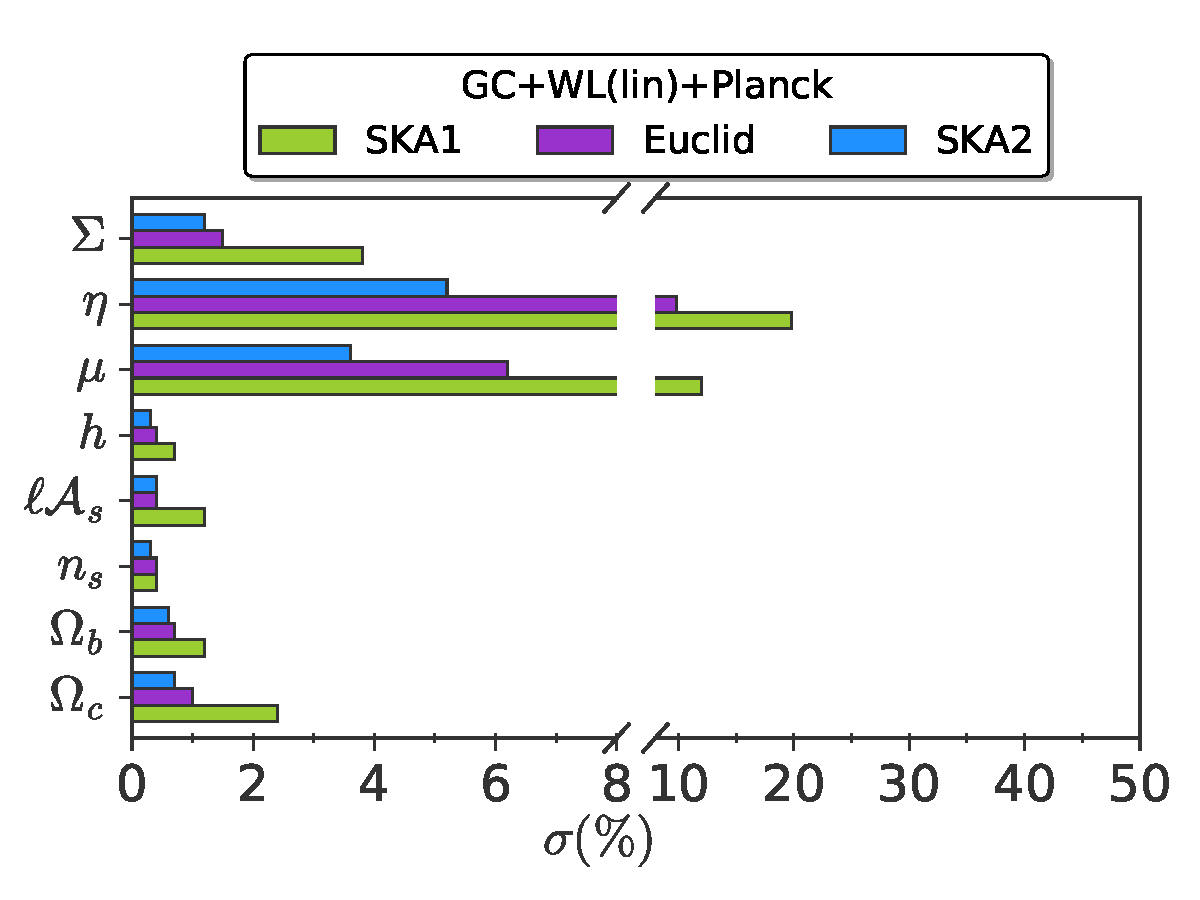
\includegraphics[width=0.45\textwidth]{Chapters/linear-nonlinear-MG-forecasts/figures/BarPlots/4surveys-GC+WLlin+Planck-MGDE-latetime}

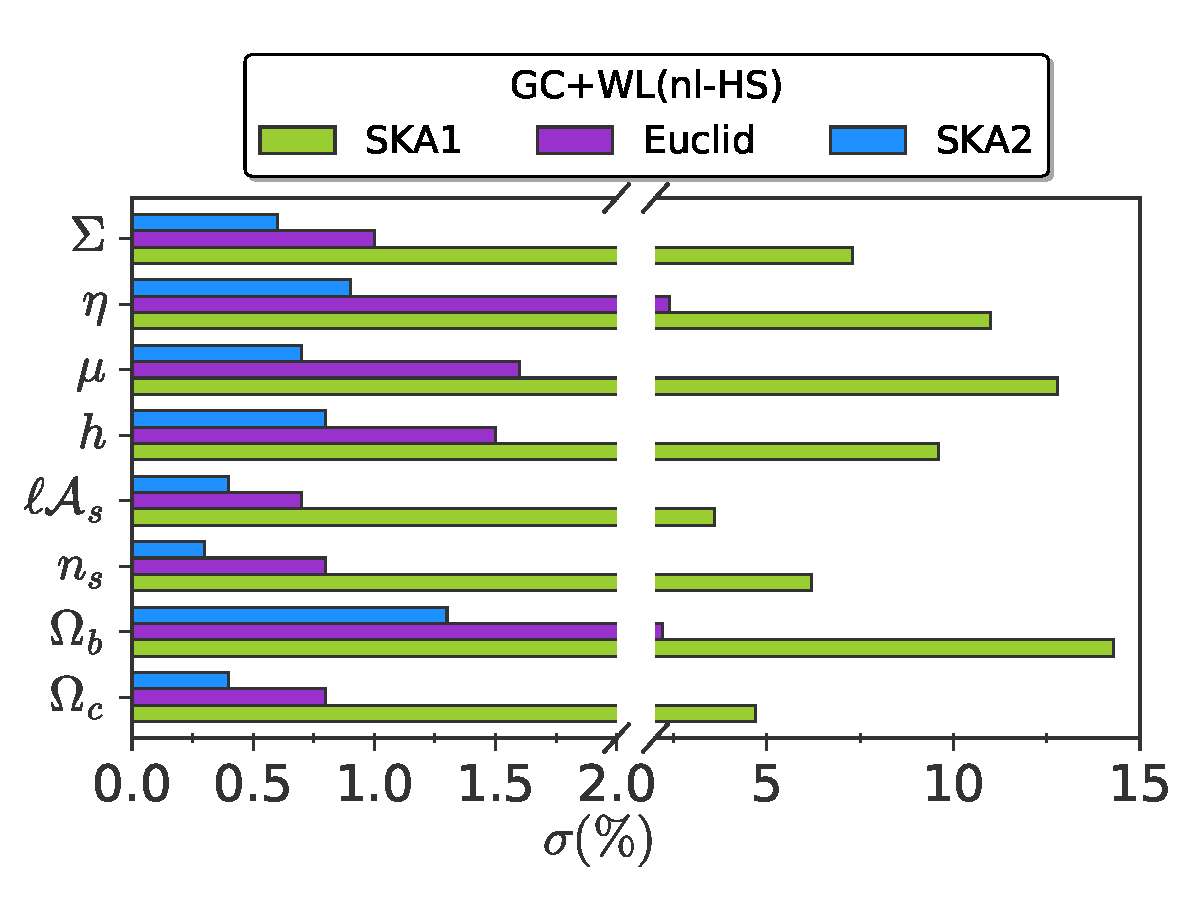
\includegraphics[width=0.45\textwidth]{Chapters/linear-nonlinear-MG-forecasts/figures/BarPlots/4surveys-GC+WLnlHS-MGDE-latetime}\hspace{-0.5pt}
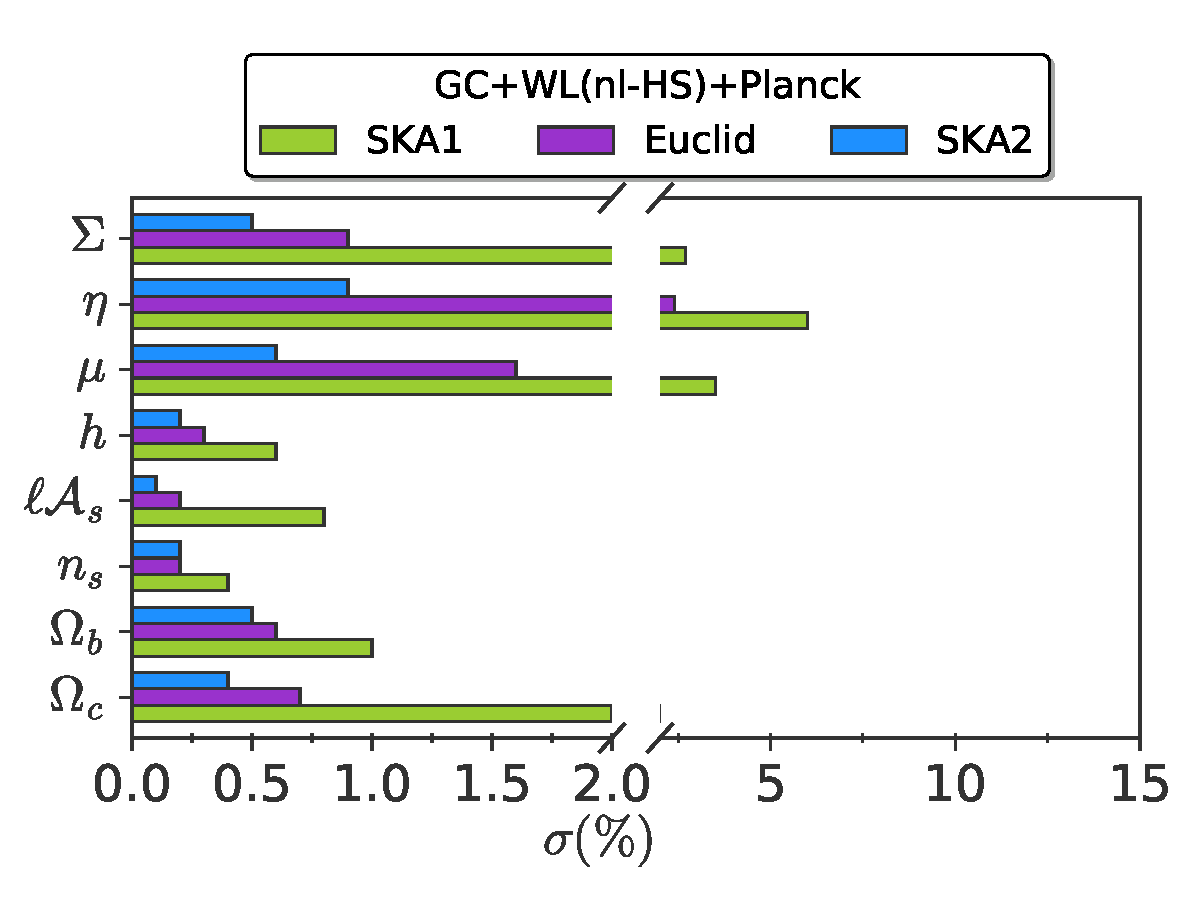
\includegraphics[width=0.45\textwidth]{Chapters/linear-nonlinear-MG-forecasts/figures/BarPlots/4surveys-GC+WLnlHS+Planck-MGDE-latetime}
\par\end{centering}
\caption[Comparison of 1$\sigma$ errors on cosmological parameters for GC, WL and Planck for future surveys in the late-time parametrization.]{\label{fig:BarPlot-DE-GC-1}1$\sigma$ fully marginalized errors
on the parameters $\{\Omega_{m},\Omega_{b},h,\ell\mathcal{A}_{s},n_{s},\mu,\eta,\Sigma\}$ 
for the late-time parameterization of MG obtained by forecasts on
Galaxy Clustering (non-linear HS) (top left panel), Weak Lensing (non-linear HS) (top right panel), the 
combinations GC+WL (linear) (middle left) and GC+WL+{\it Planck} (linear) (middle right) and
the combinations GC+WL (non-linear HS) (bottom left) and GC+WL+{\it Planck} (non-linear) (bottom right).
In the GC case, the surveys
considered are SKA2 (blue), SKA1-SUR (green), Euclid Redbook (purple) and DESI-ELG (orange). For forecasts including WL, only Euclid, SKA1 and SKA2 are included.
Although the 1$\sigma$ constraints on the standard parameters are overall weaker for WL than for GC, Weak Lensing surveys perform better on Modified Gravity parameters. Comparing the different surveys,
Euclid and SKA2 perform similarly well for the WL observable alone, if non-linearities are included.
Notice that SKA1-SUR performs better than Euclid on the $\eta$ and $\Sigma$ parameters, because it can measure better at lower redshifts.
Including the \planck\ prior, the GC+WL combination for Euclid and SKA2 constrains all parameters at much better than percent accuracy. 
Detailed specifications of the different surveys are explained in the text.
}
\end{figure}

For the SKA1 and SKA2 surveys (whose specifications are explained in detail in  \cref{sub:FutureSurveys}) 
\done\todo{fix this} 
previous work on forecasting cosmological parameters has been done, among others, by \cite{baker_observational_2015} and \cite{bull_extending_2015}. 
In the latter work, the author parameterizes the evolution of $\mu(a)$ using the late-time parameterization, but also adds an extra parameter
allowing for a scale dependence in $\mu(a)$ and including a \planck\ prior. For a fixed scale,
the 1$\sigma$ errors on the amplitude of $\mu$ lie between 0.045 and 0.095, depending on the details of the SKA1 specifications, while  
for SKA2, this error is of about 0.017. This setting would correspond to our GC+WL(linear) + \planck\ case 
(see Table \ref{tab:errors-GC-SKAcompare-MG-DE-mu-eta-sigma}) where we find for SKA1 a 1$\sigma$ error on $\mu$ of 0.12 and for SKA2 the forecasted error is 0.036.
Our errors are somewhat larger, but we also have extended our analysis to let the gravitational slip $\eta$ be different from 1 at present time, our departure from $\mu=1$ at present time is larger by a factor 4 and 
our linear forecast is conservative in the sense that it includes less wavenumbers $k$ at higher redshifts, compared to theirs.


In Figure \ref{fig:BarPlot-DE-GC-1} we show the 1$\sigma$ fully
marginalized forecasted errors on the parameters 
$\{\Omega_{m},\Omega_{b},h,\ell \mathcal{A}_{s},n_{s},\mu,\Sigma\}$
for different Weak Lensing (left panel) and Galaxy Clustering (right panel)
surveys in the late-time parameterization. In the GC case, the surveys
considered are DESI-ELG (yellow), SKA2 (green), SKA1-SUR (orange)
and Euclid (blue). For the WL forecast, we considered Euclid (blue),
SKA1 (orange) and SKA2 (green). These constraints correspond to the ones
listed in \cref{tab:errors-GC-SKAcompare-MG-DE-mu-eta-sigma}. 
The marginalized confidence contours for the $\mu$-$\eta$ plane , 
comparing all these surveys, can be seen in the left panel of \cref{fig:combined_surveys}.
The 1$\sigma$ fully marginalized
constraints on the parameters are weaker for WL than for GC,
which may be a consequence of the higher correlation among variables
for the Weak Lensing observable, described in the previous  \cref{subsub:late-time-comb-GC+WL}.
Comparing the different surveys,
the general trend is that Euclid and SKA2 perform at a similar level for WL at both linear and non-linear level; for GC and when combining both probes, SKA2
gives the strongest constraints, followed by Euclid, SKA1 and DESI (for GC).
Notice that in this parameterization, a SKA1-SUR GC survey constrains
the $\Sigma$ parameter alone better than a Euclid Galaxy Clustering
survey (although Euclid is overall much stronger as can be seen with the FoM). This is due to the fact that SKA1-SUR probes much lower
redshifts (from $z=0.05-0.85$) than Euclid and is therefore suitable to better constrain those parameterizations in which the effect of the Modified Gravity parameters is stronger at lower redshifts; this is the case of the late-time parameterization, which is proportional
to the dark energy density, dominating at low redshifts only. This result is reversed in the early time parameterization, in which Modified Gravity can play a role also at earlier redshifts. 


\begin{figure}[htbp]
\centering
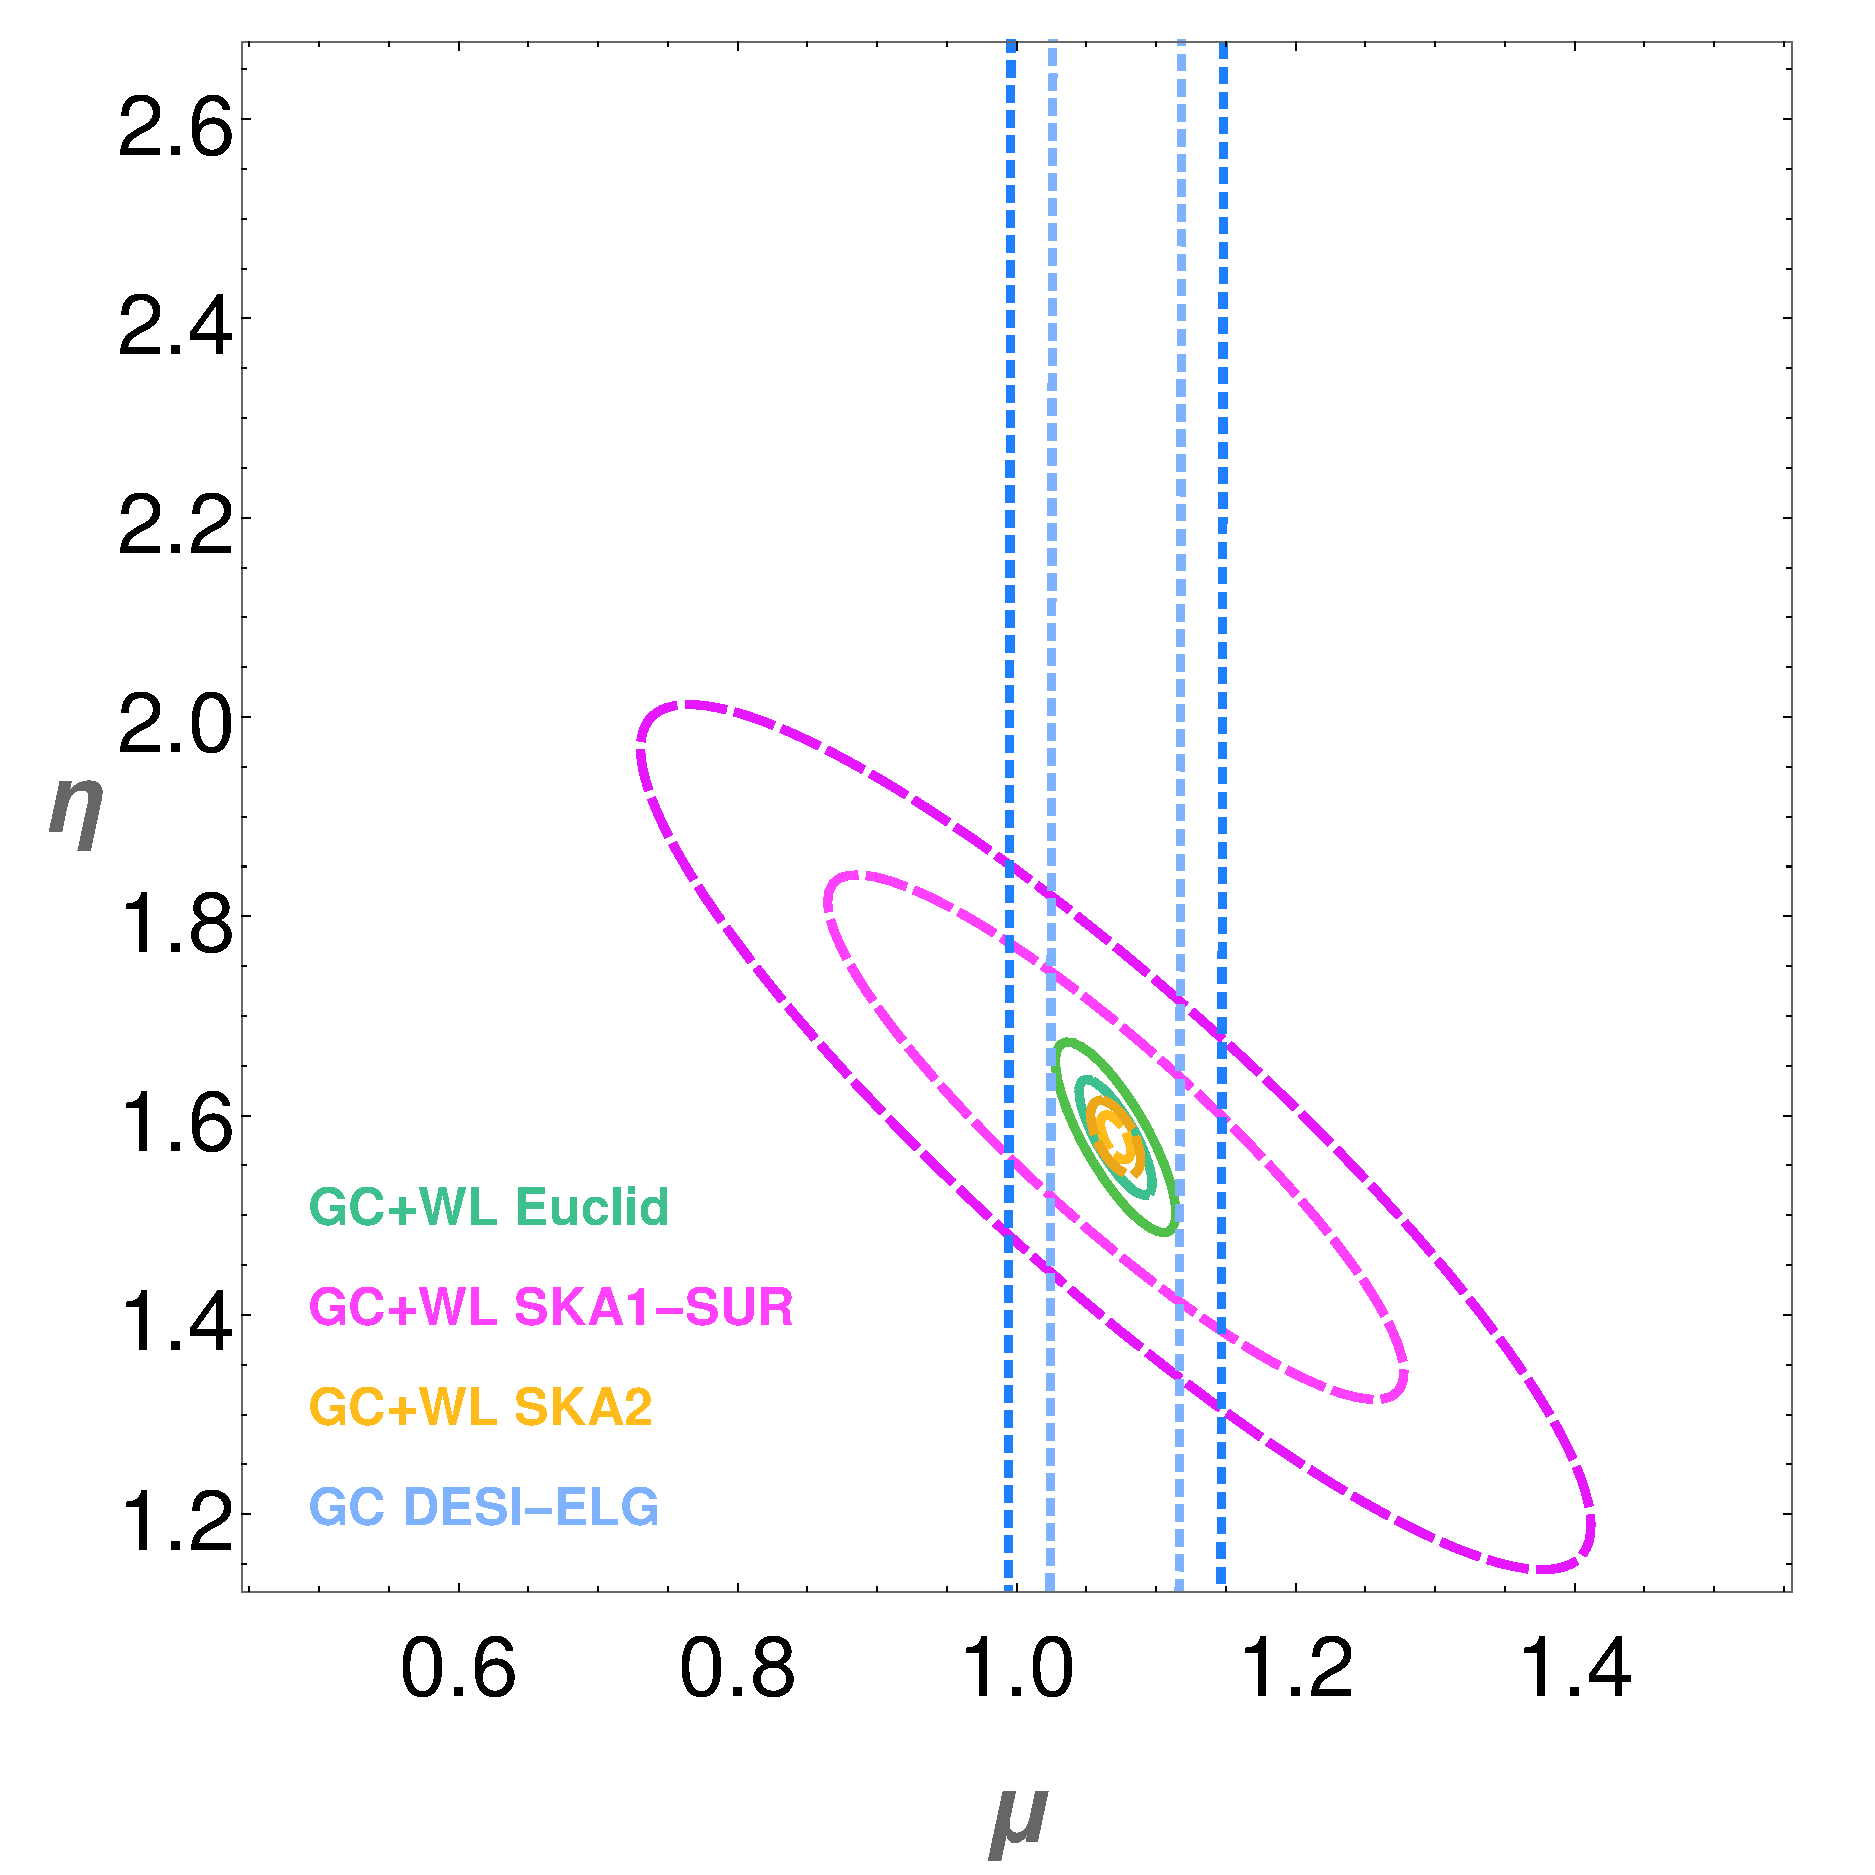
\includegraphics[width=0.45\linewidth]{Chapters/linear-nonlinear-MG-forecasts/figures/ellipses/DE-related/ellipsesPlot-withLegend-Ska2-SKA1-Euclid-DESI-MuEtaFisher-Marged-fiducialMGDE2nonuhs-GC+WL--nlHS-pars-6-7_-FixedRange.pdf}
\includegraphics[width=0.45\linewidth]{Chapters/linear-nonlinear-MG-forecasts/figures/ellipses/T-related/ellipsesPlot-withLegend-MuEtaFisher-Marged-AllSurveys-SKA1-SKA2-Euclid-DESI-fiducialMGTR2nonuhs-GC_GC+WL--nlHS-pars-6-7_-FixedRange.pdf}
\caption[Fisher confidence contours for future surveys in the late- and early-time parameterizations.]{\label{fig:combined_surveys}
1$\sigma$ and 2$\sigma$
fully marginalized confidence contours on the parameters
$\mu$ and $\eta$, for 3 different surveys combining Galaxy Clustering (GC) and Weak Lensing (WL): Euclid, SKA1-SUR
and SKA2 and for GC only: DESI-ELG, all in the late-time (left panel) and early-time (right panel) parameterizations
of sections \ref{sub:MG-DE} and \ref{sub:MG-TR}, respectively.
As explained in the main text, the constraints are parameterization-dependent, especially on $\eta$, where in
the late-time scenario GC alone is not able to constrain it, while in the early-time scenario GC can constrain both $\mu$ and $\eta$.
}
\end{figure}

\subsection{\label{sub:MG-TR} Modified Gravity in the early-time parameterization}

\subsubsection{Galaxy Clustering, Weak Lensing and its combination}

We extend our analysis now to an alternative choice, the early time parameterization specified in Eqns.\ (\ref{eq:TR-mu-parametrization}) and (\ref{eq:TR-eta-parametrization}). As before, we use
Euclid Redbook specifications for WL and GC
and the cut in scales discussed previously for the two observables, i.e. 
a maximum wavelength cutoff at $k_{\rm max}=0.15$ for GC and a maximum multipole of $\ell_{\rm max}=1000$ for WL in the 
linear case, and a cutoff $k_{\rm max}=0.5$h/Mpc and a maximum multipole of $\ell_{\rm max}=5000$ for WL in the non-linear regime,
which is analyzed using the prescription described in Sec.\ \ref{sub:Prescription-HS}.
We use the two observables both separately and in combination, without accounting for cross correlation of the two (as discussed in section \ref{sec:Results:-Redshift-Binned} this seems to correspond to a conservative choice), 
with and without \planck\ priors.

Results are shown in Table \ref{tab:errors-Euclid-GC-WL-early_time} and 
Figure \ref{fig:T-related-ellipses-mu-omegac}.
The general behaviour of the constraints is similar to the one in the late-time parameterization,
with the combination of GC and WL able to break the degeneracies with standard cosmological
parameters, leading to a significant improvement of the constraints on MG parameters, constraining $\mu$ and $\Sigma$ at the 1-2\% level. 
There are some other interesting differences with the late-time scenario. 
First, the addition of \planck\ priors does not really improve much the constraints obtained by GC or WL alone, which was not the case in the 
late-time parametrization. This is related to the fact that in the early-time parameterization, GC and WL (non-linear) on their own are already good at constraining both
$\mu$ (at 2-3 \%) and $\eta$ (at around 8\%), with consequently small errors on $\Sigma$ ($\approx 3$\%).
In \cref{sec:appder} we show the derivatives of the matter power spectrum with respect to the MG parameters $\mu$ and $\eta$ in both
parameterizations. We can observe that in the early-time scenario, the derivative  $dP(k)/d\eta$ is larger than in the late-time
parameterization, leading therefore to better constraints.
Another difference lies in the correlation among parameters, which for WL and GC+WL is considerably smaller than in the late-time scenario. 
The Figure of Correlation (defined in \cref{eq:FoC}) for GC (non-linear HS) alone is 4.7, while
for WL (non-linear HS) the correlation is somewhat higher, with $\textrm{FoC}=7.3$.
When combining both probes (GC+WL (non-linear HS)) the FoC goes to an intermediate point of 5.2.

\begin{figure}[htbp]
\centering{}
\includegraphics[width=0.45\textwidth]{Chapters/linear-nonlinear-MG-forecasts/figures/ellipses/T-related/ellipsesPlot-withLegend-Manual-MuEtaFisher-Marged-fiducialMGTR2nonuhs-GC_WL_GC+WL+Planck--nlHS-pars-6-7_-.pdf}
\includegraphics[width=0.45\textwidth]{Chapters/linear-nonlinear-MG-forecasts/figures/ellipses/T-related/ellipsesPlot-noLegend-Manual-MuSigmaFisher-Marged-fiducialMGTR2nonuhs-GC_WL_GC+WL+Planck--nlHS-pars-6-7_-.pdf}
\\
\includegraphics[width=0.45\textwidth]{Chapters/linear-nonlinear-MG-forecasts/figures/ellipses/T-related/ellipsesPlot-noLegend-Manual-MuSigmaFisher-Marged-fiducialMGTR2nonuhs-GC_WL_GC+WL+Planck--nlHS-pars-2-6_-.pdf}
\includegraphics[width=0.45\textwidth]{Chapters/linear-nonlinear-MG-forecasts/figures/ellipses/T-related/ellipsesPlot-noLegend-Manual-MuSigmaFisher-Marged-fiducialMGTR2nonuhs-GC_WL_GC+WL+Planck--nlHS-pars-4-7_-.pdf}
\caption[1$\sigma$ marginalized confidence contours for Euclid GC, WL and Planck in the early-time parameterization.]{\label{fig:T-related-ellipses-mu-omegac} Fisher Matrix marginalized forecasted contours
(1$\sigma$, 2$\sigma$) for the Euclid Redbook satellite in the early-time
parameterization using mildly non-linear scales and the HS prescription.
Green lines represent constraints from the Galaxy Clustering survey,
pink lines stand for the Weak Lensing observables, and orange lines represent the
 GC+WL+{\it Planck} combined confidence
regions. \textbf{Upper left: }contours for the fully marginalized
errors on $\eta$ and $\mu$. \textbf{Upper right: }contours for the
fully marginalized errors on $\Sigma$ and $\mu$.\textbf{ Lower left:
}contours for the fully marginalized errors on $\mu$ and $\Omega_{b}$.
\textbf{Lower right: }contours for the fully marginalized errors on
$\Sigma$ and $\ln 10^{10} A_s$. Notice that in this parameterization, GC and WL are able to constrain both $\mu$ and
$\eta$ or $\Sigma$ on their own.}
\end{figure}





\subsubsection{Other Surveys: DESI-ELG, SKA1 and SKA2 \label{subsub: other-surveys-early-time}}

Also in the early time parameterization we obtain
the 1-$\sigma$ fully marginalized errors for Galaxy Clustering (top left
panel of Figure \ref{fig:BarPlot-MGTR-Surveys}) considering DESI-ELG
(yellow), SKA2 (green), SKA1-SUR (orange) and Euclid (blue), and for
Weak Lensing (top right panel of Figure \ref{fig:BarPlot-MGTR-Surveys})
using Euclid (blue), SKA1 (orange) and SKA2 (green). We also report
the results in Table \ref{tab:errors-GC-SKAcompare-MG-TR-mu-eta-sigma-Zhao-1},
where it is possible to notice how the conclusions drawn on the hierarchy
 of the considered experiments do not change
with respect to the late-time parameterization. The main difference
is that in this case the full SKA1-SUR GC survey does not
constrain the $\Sigma$ parameter better than the Euclid survey; this
is due to the fact that in the early time parametrization, deviations
from $\Lambda$CDM are present also at high redshift, therefore we
do expect the information present at small redshift to be as relevant
as the one coming from higher $z$, where Euclid performs significantly
better than SKA1-SUR. The marginalized contours for the $\mu$-$\eta$ plane, 
comparing all these surveys, can be seen in the right panel of Fig.\ref{fig:combined_surveys}.



\begin{figure}[htbp]
\begin{centering}
\includegraphics[width=0.45\textwidth]{Chapters/linear-nonlinear-MG-forecasts/figures/BarPlots/4surveys-GCnlHS-MGTR-earlytime}\hspace{-0.5pt}
\includegraphics[width=0.45\textwidth]{Chapters/linear-nonlinear-MG-forecasts/figures/BarPlots/4surveys-WLnlHS-MGTR-earlytime.pdf}

\includegraphics[width=0.45\textwidth]{Chapters/linear-nonlinear-MG-forecasts/figures/BarPlots/4surveys-GC+WLlin-MGTR-earlytime}\hspace{-0.5pt}
\includegraphics[width=0.45\textwidth]{Chapters/linear-nonlinear-MG-forecasts/figures/BarPlots/4surveys-GC+WLlin+Planck-MGTR-earlytime}

\includegraphics[width=0.45\textwidth]{Chapters/linear-nonlinear-MG-forecasts/figures/BarPlots/4surveys-GC+WLnlHS-MGTR-earlytime}\hspace{-0.5pt}
\includegraphics[width=0.45\textwidth]{Chapters/linear-nonlinear-MG-forecasts/figures/BarPlots/4surveys-GC+WLnlHS+Planck-MGTR-earlytime}
\par\end{centering}
\caption[Comparison of 1$\sigma$ errors on cosmological parameters for GC, WL and Planck for future surveys in the late-time parametrization.]{\label{fig:BarPlot-MGTR-Surveys} Same as Fig.\ref{fig:BarPlot-DE-GC-1} but for the early-time parameterization (Eqns. \ref{eq:TR-mu-parametrization},\ref{eq:TR-eta-parametrization})
The 1$\sigma$ fully marginalized
constraints on the parameters are weaker for WL than for GC,
which is a consequence of the higher correlation among variables
for the Weak Lensing observable. 
}
\end{figure}


\section{Modified Gravity in the Effective Field Theory formalism \label{sec:EFT-forecasts}}

\footnote{This section is not contained in the publication \cite{casas_linear_2017}, 
but will be the subject of a future work.}
In this section we show some forecasts for the 
constraints that can be obtained on the parameters of a simple model within the Effective Field Theory  (EFT) formalism. We simulate a Galaxy Clustering Euclid survey and test the difference between applying linear and non-linear power spectra. 

The EFT action was presented in \cref{sub:EFT-of-DE}, where we described the 6 free 
functions of time that characterize this formalism, which is able to recover all theories of a 
scalar field plus GR at the linear perturbation level.
Following the example of the \planck paper \cite{planck_collaboration_planck_2016-7},
as we have done in the previous two parameterizations,
we will reduce considerably the freedom contained in the EFT Lagrangian.
From the 6 free functions available in \cref{eq:EFT-funcs}, we will demand that
$\bar{M}_3^2 = \bar{M}_2^2$, which implies that $\alpha_T = 0$, so that gravitational waves 
propagate with the speed of light. In order to remain within the ``Horndeski``
class of models, we further impose $\alpha_H = 0$. Furthermore, to simplify
our model, we will set $\bar{M}_3^1 = \bar{M}_2^4 = 0$, which in terms of the $\alpha$
functions, implies: $\alpha_M = - \alpha_B$. 
Therefore, we will consider a very limited model, which basically
reduces to a non-minimally coupled k-essence model (see \cite{amendola_dark_2010}, for a review). Nevertheless,
this model offers an interesting phenomenology that modifies the gravitational
potentials at large and small scales.

In addition to
the standard cosmological parameters, we have now just a free function $\alpha_{M}$,
which can be linked to the operator $\Omega(a)$ in \cref{eq:EFT-funcs}, through: 
\begin{equation}
\alpha_{M}(a)=\frac{a}{\Omega(a)+1}\frac{\mbox{d}\Omega(a)}{\mbox{d}a}\label{eq:alphama}
\end{equation}
In order to reduce this function in a parametric form, we use a scaling
ansatz and set $\alpha_{M}=\alpha_{M0}a^{\beta}$, where the subscript
$0$ indicates the value today. For $\beta>0$ the modification of
gravity decreases in the past. Integrating equation \ref{eq:alphama},
one obtains:
\begin{equation}\label{eq:EFT-omega}
\Omega(a)=\exp\left(\frac{\alpha_{M0}}{\beta}a^{\beta}\right)-1.
\end{equation}
Therefore the free parameters in this case are $\theta_i=\{\Omega_{m},\Omega_{b},\ln(10^{10}A_{s}),n_{s},h,\alpha_{M0},\beta\}$
and as fiducial cosmology we assume the marginalized values obtained
through the analysis of Planck CMB data.

\begin{table}[htbp]
	\centering{}
	\begin{tabular}{|c|c|}
		\hline 
		\multicolumn{2}{|c|}{\Tstrut \textbf{EFT}}  \tabularnewline
		\hline
		Parameter  & Fiducial \Tstrut \tabularnewline
		\hline 
		$\Omega_{c}$  & $0.254$ \Tstrut  \tabularnewline
		$\Omega_{b}$  & $0.048$  \tabularnewline
		$n_{s}$  & $0.969$  \tabularnewline
		$\log(10^{10}A_{s})$  & $3.06$  \tabularnewline
		$h$  & $0.682$   \tabularnewline
		$\alpha_{M}$  & $0.01$ \tabularnewline
		$\beta$  & $1$ \tabularnewline
		\hline 
	\end{tabular}\protect\caption{Fiducial model used for the EFT parametrization. 
	The parameters are those allowed by the analysis in the \planck paper \cite{planck_collaboration_planck_2016-7}.}
	\label{tab:fiducial-EFT} 
\end{table}

\begin{figure}[htbp]
	\centering{}
	\includegraphics[width=0.45\textwidth]{Figures/EFT-alfa-beta.png}
	\includegraphics[width=0.45\textwidth]{Figures/EFT-alfa-h.png}
	\\
	\includegraphics[width=0.45\textwidth]{Figures/EFT-alfa-Omb.png}
	\includegraphics[width=0.45\textwidth]{Figures/EFT-h-Omb.png}
	\caption[1$\sigma$ marginalized confidence contours for Euclid GC in the EFT formalism.]{\label{fig:EFT-ellipses-mu-omegac} Fisher Matrix marginalized forecasted contours
		(1$\sigma$, 2$\sigma$, 3$\sigma$) for the Euclid Redbook satellite in the EFT model using mildly non-linear scales and the HS prescription (labeled as nonlin-Zh in the figure).
		Green lines represent linear constraints, while blue lines stand for the non-linear
		forecasts. \textbf{Upper left: }contours for the fully marginalized
		errors on $\alpha_m$ and $\beta$. \textbf{Upper right: }contours for the
		fully marginalized errors on $\alpha_m$ and $h$.\textbf{ Lower left:
		}contours for the fully marginalized errors on $\alpha_m$ and $\Omega_b$.
		\textbf{Lower right: }contours for the fully marginalized errors on
		$h$ and $\Omega_b$.
	    It can be seen quite clearly from these plots that the inclusion of non-linear
    scales improves radically the constraints on the model parameters.}
\end{figure}

In \cref{fig:EFT-ellipses-mu-omegac}, we show the marginalized confidence contours for the our EFT model, using a Galaxy Clustering Euclid survey, with Redbook specifications.
We can see in \cref{fig:EFT-ellipses-mu-omegac} that the constraints on the $\beta$ and $\alpha_m$ parameters are quite poor if one uses only linear scales to perform the forecast.
Using non-linear scales together with the non-linear HS prescription, yields constraints
which are more than one order of magnitude better. We see again, as in previous sections,
that this effect is much bigger for Modified Gravity parameters than for standard cosmological parameters.
For example in the case of the combination $h$-$\Omega_b$ in the bottom left panel of \cref{fig:EFT-ellipses-mu-omegac}, we see that the improvement when adding non-linear scales is of just a factor 
$\sim 2-3$.
The constraints on $\beta$ and $\alpha_m$ are relatively good for a non-linear forecast, but we have to take into account that we are imposing a very particular parameterization in \cref{eq:EFT-omega}.

We leave for a future work the study of a redshift-binned parameterization within the EFT formalism.

\section{Effect of the Hu-Sawicki non-linear prescription on the forecasts
\label{sub:Testing-the-effect-of-Zhao}}

In this section we show the effect of changing the parameters $\cnl$
and $s$ used in the HS prescription (specified in Eq.\ \ref{eq:PHSDefinition})
for the mildly non-linear matter power spectrum. As mentioned already
in Section \ref{sub:Prescription-HS}, previous works (see
\cite{zhao_modeling_2014,zhao_n-body_2011,koyama_non-linear_2009}),
have fitted the values of $\cnl$ and $s$ to match N-body simulations
in specific Modified Gravity models. In all these cases the HS parameters
$\cnl$ and $s$ have been found to be of order unity, with $\cnl$
ranging usually from $0.1$ to $3$ and $s$ from about $1/3$ to
a value of around $2$. In the absence of N-body simulations for our
models, we selected our benchmark HS parameters
to be $\cnl=1$ and $s=1$, as discussed in Section \ref{sub:Prescription-HS}, which we used
for all the analysis presented above. However, in order to test
the effect of a change of $c_{nl}$ and $s$ non-linear parameters on our estimation of errors
on the cosmological parameters, we perform our GC and WL forecasts on the
MG late-time model (Section \ref{sub:MG-DE}) also changing one at
a time the values of both HS parameters. We use the following values
for our test: $\cnl=\{0.1,0.5,\,1,\,3\}$ and $s=\{0,\,1/3,\,2/3,\,1\}$.

\begin{figure}[htbp]
\centering{}
\includegraphics[width=0.45\textwidth]{Chapters/linear-nonlinear-MG-forecasts/figures/DensityPlots/GC-Zhao-effect-mu.pdf}
\includegraphics[width=0.45\textwidth]{Chapters/linear-nonlinear-MG-forecasts/figures/DensityPlots/GC-Zhao-effect-eta.pdf}
\caption[Effect of the HS non-linear prescription on parameter estimation for GC in MG.]{\label{fig:Density-GC-HSpars}Effect
of the $\cnl$ and $s$ parameters
on the 1$\sigma$ marginalized error of the $\mu$ (left panel) and the
$\eta$ (right panel) parameters
in the MG late-time parametrization for a Euclid Galaxy Clustering
forecast with Redbook specifications. The colored contours show the percentage discrepancy when
departing from the benchmark case $\cnl=1$ and $s=1$ (marked with
a black arrow) to all other points in the $\cnl$-$s$
space. The red (blue) contours signal the regions of maximum positive (negative) discrepancy.
For example in the left panel, choosing $\cnl$ and $s$ in the
red region, will yield a 1$\sigma$ marginalized error on $\mu$
which is 90\% larger than in the benchmark case (see Table
\ref{tab:errors-Euclid-GC-WL-late_time}
for the benchmark forecast). For the standard $\lcdm$ cosmological
parameters (not shown here) the discrepancy is smaller than 4\% for all choices of $\cnl$ and $s$.
}
\end{figure}


\begin{figure}[htbp]
\centering{}
\includegraphics[width=0.45\textwidth]{Chapters/linear-nonlinear-MG-forecasts/figures/DensityPlots/WL-Zhao-effect-mu.pdf}
\includegraphics[width=0.45\textwidth]{Chapters/linear-nonlinear-MG-forecasts/figures/DensityPlots/WL-Zhao-effect-Sigma.pdf}
\caption[Effect of the HS non-linear prescription on parameter estimation for WL in MG.]{\label{fig:Density-WL-HSpars}
Same as Fig.\ref{fig:Density-GC-HSpars} but for a Weak Lensing Euclid forecast using Redbook specifications.
In the left panel, choosing $\cnl$
and $s$ in the red region, will yield a 1$\sigma$ marginalized
error on $\mu$ which is 60\% larger than in the benchmark case
(see Table \ref{tab:errors-Euclid-GC-WL-late_time}
for the benchmark forecast). In the right panel we see that for the MG parameter $\Sigma$ the maximum positive and negative discrepancy
is only of about 6\%. The maximum and minimun discrepancy for the MG parameter $\eta$ is of -15\% and 50\%. This means that
the parameter $\Sigma$ (defined as the lensing Weyl potential, and therefore directly constrained by Weak Lensing) 
is much less sensitive to changes in the non-linear prescription parameters.}
\end{figure}


In Figure \ref{fig:Density-GC-HSpars} we show
the percentage discrepancy between the 1$\sigma$ marginalized error
obtained on parameters in the GC non-linear HS benchmark case (see Table
\ref{tab:errors-Euclid-GC-WL-late_time}
for the exact values) and the corresponding error obtained by performing
the same forecast with a different value of the $\cnl$-$s$ parameters.
In general terms we see that for the MG parameter $\mu$
(left panel of Figure \ref{fig:Density-GC-HSpars}) the relative difference
in the estimation of the 1$\sigma$ forecasted errors can lie between
90\% (at $\cnl=3$, $s=0.33$) and -30\% for $\cnl=0.1$ and $s=1.0$.
The behavior of the contour lines shows us that for a fixed value of $\cnl$, 
the forecasted error on the parameter $\mu$ remains unaffected.
For $\eta$ (right panel) the relative discrepancy lies between
40\% and -2\%. Here, to get the same 1$\sigma$ errors on $\eta$, one would have to vary 
both $\cnl$ and $s$.
We also tested the effect on the standard $\lcdm$ parameters and found it to be smaller than
4\% for all choices of $\cnl$ and $s$.
In the case of WL forecasts, we perform the same tests, which are shown in Figure \ref{fig:Density-WL-HSpars}.
We can observe that the relative discrepancies in the case of the
$\mu$ parameter lie between $\sim$60\% and $\sim$-15\%, while for $\Sigma$ the discrepancy is considerably smaller. 
The 1$\sigma$ error on $\Sigma$ varies only between $\pm 6$\%.
This is however a particular effect of choosing $\Sigma$, which is the true WL observable.
If we perform this test on $\eta$ using WL, we will find a stronger discrepancy,
that lies in between $\sim$50\% and $\sim$-15\%, similar to the one found for $\mu$.
 

We can also test the effect of adding these two HS parameters as extra
nuisance parameters to our model of the non-linear power spectrum;
therefore, by taking derivatives of the observed power spectrum with
respect to these parameters, we can forecast what would be the estimated
error on $\cnl$ and $s$. Then, marginalizing over $\cnl$ and
$s$ would yield more realistic constraints on our cosmological parameters,
and take into account our ignorance on the correct parameters
of the HS prescription. In Table
\ref{tab:errors-GC+WL-Marginalize-HS-Zhao-Euclid-DEpar-muetasigma}
we list the 1$\sigma$ marginalized constraints on $\cnl$ and
$s$ for our benchmark fiducial ( $\cnl=1$, $s=1$) and using the
standard fiducial for the cosmological parameters used previously
for the MG late time parametrization.

Taking these HS parameters into account in our Fisher forecast, will
automatically change the constraints on the other parameters. For our
method to be consistent, we would like this effect to remain as small
as possible. In Table
\ref{tab:errors-GC+WL-Marginalize-HS-Zhao-Euclid-DEpar-muetasigma},
we list the same constraints reported in Table
\ref{tab:errors-Euclid-GC-WL-late_time},
but obtained marginalizing over $\cnl$ and $s$ at the benchmark
fiducial $\cnl=1$, $s=1$. Comparing the two tables, we can
see that for GC the errors on the cosmological parameters remain quite
stable, except for
$\eta$ and $\Sigma$; this is understandable since those parameters
are not well constrained by GC alone. For WL, we see a difference
of 4 to 7 percent points in the errors on $h$, $n_{s}$ and $\Omega_{b}$,
while all other errors remain stable, with $\Sigma$ varying less
than 2 percent points.
Remarkably, the combined constraints from GC+WL are even less affected by the two nuisance parameters.
Comparing the Modified Gravity FoM between the two tables, shows the expected behavior, the MG FoM is reduced
when adding two extra parameters, but the change is very small, of just 0.3-0.5 nits.

\begin{table}[htbp]
\centering{}%
\tiny
\begin{tabular}{|c|c|c|c|c|c||c|c|c||c|c|c|}
\hline 
\textbf{Euclid} (Redbook)  & $\Omega_{c}$  & $\Omega_{b}$  & $n_{s}$  &
$\ell\mathcal{A}_{s}$  & $h$  & $\mu$  & $\eta$  & $\Sigma$ \Tstrut &
$\cnl$  & $s$ & MG FoM \tabularnewline
\hline 
\Tstrut Fiducial  & {0.254}  & {0.048}  & {0.969}  & {3.060}  & {0.682}  & {1.042}  & {1.719}  & {1.416}  & {1}  & {1} & relative \tabularnewline
\hline
\hline
\Tstrut \textbf{GC(nl-HS)}  & 1.0\% & 2.8\% & 1.3\% & 1.1\% & 2.0\% & 1.7\% & 784\% & 480\% & 372\% & 236\% 
& 2.4 \tabularnewline 
\Tstrut \textbf{WL(nl-HS)}   & 6.5\% & 25\% & 8.3\% & 9.1\% & 19\% & 25\% & 46\% & 6.0\% & 1680\% & 899\% 
& 4.2 \tabularnewline 
\Tstrut \textbf{GC+WL(nl-HS)} & 1\% & 2.8\% & 1.2\% & 1\% & 1.9\% & 1.6\% & 2.6\% & 1.2\% & 333\% & 166\%  
& 8.5 \tabularnewline
\hline 
\end{tabular}
\small
\protect\caption[1$\sigma$ forecasted errors on the cosmological parameters for a Euclid GC and WL survey, marginalizing over
the HS non-linear prescription parameters.]{\label{tab:errors-GC+WL-Marginalize-HS-Zhao-Euclid-DEpar-muetasigma}
1$\sigma$ fully marginalized errors on the cosmological parameters
and the two HS parameters $\cnl$ and $s$ for a Euclid Galaxy
Clustering forecast, a Weak Lensing forecast and the combination of
both in the late-time parameterization of Modified Gravity using non-linear
scales and the HS prescription. In contrast to Table
\ref{tab:errors-Euclid-GC-WL-late_time} (where $c_{nl}$ and $s$ had been fixed to the benchmark value)
here we include $\cnl$ and $s$ as free parameters
and marginalize over them. The MG FoM is computed relative to the same Euclid Redbook GC 
linear case,
used previously. The errors and the MG FoM show the expected behavior
of adding two nuisance parameters, and remain quite stable. All other naming conventions are the
same as for Table \ref{tab:errors-Euclid-GC-WL-late_time}. Remarkably, the combination of GC and WL is still able to constrain all Modified Gravity parameters at the level of 1-2 $\%$ after marginalizing over the non-linear parameters.}
\end{table}
\normalsize

\done\todo{Add EFT plot}








\section{Conclusions}



We study in this chapter the constraining power of upcoming large scale surveys on Modified Gravity theories, choosing a phenomenological approach that does not require to specify any particular model. To this purpose we consider the two functions $\mu$ and $\eta$ that encode general modifications to the Poisson equation and the anisotropic stress.
We study three different approaches to MG: redshift-binning, where we discretize the functions $\mu(z)$ and $\eta(z)$ in 5 redshift bins and 
let the values of $\mu$ and $\eta$ in each of the bins vary independently with respect to the others; an early-time parameterization, where $\mu$ and $\eta$ are allowed to vary at early times and their amplitude
can be different from unity today; a late-time parameterization where  $\mu$ and $\eta$ are linked to the energy density of dark energy and therefore they are very
close to unity in the past, but they can vary considerably at small redshifts.
% For convenience, we summarize all results in Table \ref{table_results}, with a direct link to the section and tables related to each scenario.

%\begin{table}
%\begin{tabular}{|l|l|l|} 
%\hline 
%\Tstrut \textbf{Model} & \textbf{Description} & \textbf{Results} \\ 
%\hline 
%\Tstrut Redshift Binned $\mu$ and $\eta$ & Section \ref{sub:param-z-bins-th}, Eqns.\ (\ref{eq:MGbin-mu-parametrization})-(\ref{eq:MGbin-muderiv-parametrization})  & Table \ref{tab:errors-all-MGBin3}; \,\,\,\,\,\,\,Figs.\ \ref{fig:GCcorr}-\ref{fig:GC+WL+Planck-bestconst-errspq} \\ 
%\hline 
%\Tstrut Late-time parameterization & Section \ref{sub:param-smooth-funct}, Eqns.\ (\ref{eq:DE-mu-parametrization})-(\ref{eq:DE-eta-parametrization}) & Tables \ref{tab:errors-Euclid-GC-WL-late_time},\ref{tab:errors-GC-SKAcompare-MG-DE-mu-eta-sigma}; Figs.\ \ref{fig:DE+Planck-ellipses-mu-sig-eta}, \ref{fig:BarPlot-DE-GC-1}, \ref{fig:combined_surveys} \\ 
%\hline 
%\Tstrut Early-time parameterization & Section \ref{sub:param-smooth-funct}, Eqns.\ (\ref{eq:TR-mu-parametrization})-(\ref{eq:TR-eta-parametrization}) & Tables \ref{tab:errors-Euclid-GC-WL-early_time},\ref{tab:errors-GC-SKAcompare-MG-TR-mu-eta-sigma-Zhao-1}; Figs.\ \ref{fig:T-related-ellipses-mu-omegac}, \ref{fig:BarPlot-MGTR-Surveys}, \ref{fig:combined_surveys} \\ 
%\hline 
%\Tstrut Effect of non-linear prescription & Section \ref{sub:Prescription-HS}, Eqns.\ (\ref{eq:PHSDefinition}),(\ref{eq:prescription_sigma_def}) & Table \ref{tab:errors-GC+WL-Marginalize-HS-Zhao-Euclid-DEpar-muetasigma}; \,\,\,\,\, Figs.\ \ref{fig:Density-GC-HSpars}, \ref{fig:Density-WL-HSpars} \\ 
%\hline 
%\end{tabular}
%\caption{Summary of results for this work. For each studied model, we indicate where to find the explanations and where to find the main Fisher forecast results.} \label{table_results}
%\end{table}


We use the predictions of linear perturbation theory to compute the linear power spectrum in Modified Gravity and then
use a prescription to add the non-linearities, by interpolating between Halofit non-linear corrections computed for the linear power spectrum for the MG model and for the corresponding GR model ($\eta=\mu=1$). We find that the non-linear power spectrum is sensitive to 
changes in $\mu$ and $\eta$; limiting the analysis to linear scales significantly reduces the constraining power on the anisotropic stress.
Using this prescription, we perform Fisher forecasts for Galaxy Clustering and Weak Lensing, taking into account linear and non-linear scales. 
We use the specifications for Euclid (using Redbook specifications), SKA1 \& SKA2 and DESI (only ELG). In addition to these surveys we also include
\planck\ priors obtained by performing an MCMC analysis with \planck\ data for the MG parametrizations considered here.

In the redshift-binned case, we find that in the linear case the $\mu_i$ and $\eta_i$ parameters are strongly correlated, while including the information coming from non linear 
scales reduces this correlation. We compute a figure of merit (FoM), given by the determinant of the $\mu$-$\eta$ part of the Fisher matrix, for the cases examined, finding that 
the combination of Galaxy Clustering and Weak Lensing is able to break the degeneracies among Modified Gravity parameters; as an example the error obtained with the non-linear prescription on $\mu$ ($\eta$) in the first redshift bin changes 
from $7\%$ ($20\%$) for Galaxy Clustering to $2.2\%$ ($3.6\%$) when this is combined with Weak Lensing, even if Weak Lensing alone is not very constraining for the same parameters. 
Overall, constraints are stronger at low redshifts, with the first two bins (0 < z < 1) being constrained at better than $5\%$ for both $\mu$ and $\eta$ if non-linearities are included (while the constraints are half as good, $<10\%$, if we only consider linear scales).

Given the significant correlation between the $\mu_i$ and $\eta_i$ parameters, we apply the ZCA decorrelation method, in order to find a set of uncorrelated 
variables, which gives us information on which redshift dependence of $\mu$ and $\eta$ will be best constrained by future surveys. If one combines GC+WL (Euclid Redbook)+{\it Planck}, the best constrained combinations of parameters (effectively $2\mu+\eta$ in the lowest redshift bin) will be measured with a precision of better than 1\%.
In the linear case, the errors on the decorrelated $q_i$ parameters are about 2 orders of magnitude smaller than for the primary parameters, 
while in the non-linear HS case, the improvement in the errors is of one order of magnitude. This also shows that applying a decorrelation procedure is worth even when non-linearities are considered.

In addition to binning Modified Gravity functions in redshift, we also forecast the constraining power of the same probes in the case where we assume a specific time evolution for the $\mu$ and $\eta$ functions. We choose two different and complementary time evolutions, used in \cite{planck_collaboration_planck_2016} and to which we refer as late-time and early-time evolution. We investigate also in this case the impact of the non-linear prescription interpolating between Halofit and the MG power spectrum. For these parameterizations we 
extract constraints on the present reconstructed value of $\mu$,  $\eta$ and $\Sigma$, where the latter is the parameter actually measured directly by Weak Lensing.  
In the late time parameterization, in the linear case, $\mu$ is mainly constrained by GC (although poorly, at the level of $17\%$) while WL constrains directly $\Sigma$, the modification of the lensing potential, at the level of $9\%$. Adding non-linear scales allows to significantly improve constraints down to less than $2\%$ for GC (on $\mu$) and to less than $5\%$ on $\Sigma$ for those two probes. Combining probes allows to reach $1-2\%$ on all Modified Gravity values of the $\mu$,  $\eta$ and $\Sigma$ functions at z = 0.

In the early-time parameterization, we find that including non-linearities allows to constrain also the $\eta$ and $\Sigma$ functions with GC alone at the level of 8\% and 5\%, respectively. This is related to the early time 
deviations from GR allowed by this parameterization, which are not present in the late time case: a variation in $\eta$ can
yield a variation of the amplitude of the power spectrum, which can then be measured in the mildly non-linear regime.
Overall, also in this case the combination of Weak Lensing and Galaxy Clustering leads to errors of the order of $1\%$ on the
values of these functions at present. 


Finally, we test the impact on the forecasts given by uncertainties appearing in the non linear HS prescription, related in particular to the parameters $c_{nl}$ and $s$. We find that
the errors on the parameters $\mu$ and $\eta$ can vary by up to 
$90\%$ for the Galaxy Clustering case and up to $65\%$ for Weak Lensing when we change the fiducial values of the HS parameters in a region between 0 and 3 for $c_{nl}$
and 0 and 1 for $s$. The effect on $\Sigma$ is quite small, with a discrepancy of $\pm 6 \%$ compared to the benchmark case.
Interestingly, when we include these two parameters as extra nuisance parameters in our forecast formalism and marginalize over them, 
the effect is very small and the errors found previously remain stable both for GC, WL and their combination.


It is clear that limiting the analysis to linear scales discards important information encoded in structure formation. On the other hand, a realistic analysis of non-linear scales would have to include several further effects (baryonic effects, higher order RSD's, damping of BAO peaks, corrections
to peculiar velocity perturbations, higher order perturbation theory in Modified Gravity, just to name a few), which make our non-linear case an optimistic limit.
Therefore, the quantitive true constraints given by a survey like Euclid will probably lie in between these two limiting cases. 
\done\todo{check for repetitions with other chaps}









  



\chapter{Forecasts for coupled dark energy in the non-linear regime \label{chap:Fitting-CDE}}


\section{Introduction}





\todo{check for repetitions}
Cosmological data have reached a level of precision that forces us
to address effects which may have been safely neglected in the past.
Among them, predicting the behaviour of theoretical models at non-linear
scales gives a more concrete chance to disentangle $\Lambda$CDM from
alternative scenarios. The non-linear power spectrum contains useful
information encoded in the clustering of galaxies and the weak lensing
correlations, which can help to constrain more tightly the cosmological
parameters and remove certain degeneracies between them. The drawback
relies in the fact that the full estimate of the non-linear power
spectrum requires time-demanding and computationally expensive N-body
simulations. As a consequence, there exist simulations only for a
handful of models beyond $\Lambda$CDM on a very limited subset of
the parameter space of dark energy theories. This makes it hard to
use the non-linear power spectrum in forecasts (see e.g.),
both when doing cosmological parameter estimation via Monte Carlo
simulations and with the simpler approximation of the Fisher matrix
formalism. The alternative is to employ fitting functions for the
non-linear power spectrum, like Halofit \citep{smith_stable_2003,takahashi_revising_2012}
or machine learning estimators like the cosmological emulator (CosmicEmu)
\citep{heitmann_coyote_2010,lawrence_coyote_2010,heitmann_coyote_2014}
and the interpolator PkANN \cite{agarwal_pkann_2012,agarwal_pkann_2014}
based on artificial neural networks. All these methods are calibrated
or trained using large sets of N-body simulations and typically permit
an exploration of the parameter space just around a fiducial $\lcdm$
cosmology or $w\mbox{CDM }$cosmology with a constant $w$. An extension
of Halofit to account for massive neutrinos was realised in \citep{bird_massive_2011},
which was then used in \citep{audren_neutrino_2013} to perform a
parameter estimation using a Markov Chain Monte Carlo technique. Other
authors have recently used polynomial fits to take into account systematic
effects in the non-linear regime like baryonic effects such as in
\cite{bielefeld_cosmological_2014} or to parametrize the cosmological
dependence of non-linear clustering, beyond the Zeldovich approximation
(see \cite{mohammed_analytic_2014}). These fitting functions have,
however, an intrinsic error that usually increases when scales become
highly non-linear; therefore one has to be aware of the range in scales
and redshifts they were designed to work on, in order to keep the
errors induced on the power spectrum under control.

As an alternative to fitting formulae and N-body simulations, there
has been in recent years a substantial progress in semi-analytical
methods to calculate the non-linear power spectrum at mildly non-linear
scales, such as for example renormalized perturbation theory \citep{crocce_renormalized_2006}
and all other resummation methods derived from it (for example \cite{Anselmi2012}),
the time renormalisation group (TRG) \citep{Pietroni_2008} and effective
field theories of large scale structure \cite{baumann_cosmological_2010}.
Most of these approaches claim to reach percent accuracy at the baryon
acoustic oscillation (BAO) scale and a bit beyond the second BAO peak,
but they are still not able to predict what happens at highly non-linear
scales, when the single stream approximation does not hold any longer.

In this paper, we will use N-Body simulations to find fitting functions
for a class of models beyond $\Lambda$CDM usually refered to as coupled
Dark Energy (CDE). These models, widely discussed in literature \citep{Wetterich_1995, Amendola_2000,Amendola_2004,pettorino_baccigalupi_2008},
involve an extra degree of freedom, associated to a scalar field that
provides acceleration and mediates a fifth force, in addition to gravity,
which is felt by dark matter particles only. Semi-analytical non-linear
analysis \cite{wintergerst_clarifying_2010,Saracco_etal_2010} and
cosmological N-body simulations within coupled Dark Energy have been
performed by many different groups \citep{baldi_etal_2010,Li_Barrow_2011,maccio_coupled_2004,carlesi_hydrodynamical_2014-1,baldi_codecs_2012,2015arXiv150407243P}
and their effects on large scale structure formation have been identified
and characterised. The power spectrum, halo mass functions and concentration,
halo spin and sphericity, voids and amount of substructures show noticeable
differences compared to a simple $\Lambda$CDM model (see for example
\citep{mainini_mass_2006,maccio_concentration_2008,baldi_clarifying_2011,cui_halo_2012,baldi_effect_2011,sutter_observability_2014}
and the review article \citep{Baldi_2012b}). For a constant coupling,
constraints have been found for a variety of probes \citep{pettorino_constraints_2012,pettorino_testing_2013,amendola_skewness_2004,Xia_2009},
with the latest ones discussed by the Planck collaboration in \citep{planckcollaboration_planck2015_2015}.
Recently there have been attempts to constrain more general couplings
between dark matter (DM) and dark energy (DE) using large-scale structure
\citep{creminelli_single-field_2014}, CMB \citep{morris_cosmicmicrowave_2014}
or laboratory experiments \citep{hamilton_atominterferometry_2015}.
Forecasts on coupled dark energy using galaxy clustering (GC) and
weak lensing (WL) measurements for future surveys like Euclid have
been discussed in \citep{amendola2012testing}, but have been performed
using only linear power spectra for the CDE models. The TRG method
has been extended to coupled Dark Energy \citep{saracco_non-linear_2010}
and to massive neutrinos \citep{lesgourgues_non-linear_2009}. However
the TRG method does not produce a reliable estimation of the power
spectrum for scales larger than $k\approx0.3h/\mbox{Mpc}$, which
makes them less suitable for forecasts which attempt to extract information
on highly non-linear scales.

The CoDECS (Coupled Dark Energy Cosmological Simulations) set of N-body
simulations \citep{baldi_codecs_2012} has shown that CDE models have
characteristic and measurable features in the morphology and history
of non-linear structures, such as halos, subhalos and voids,\textcolor{black}{{}
and therefore in the non-linear power spectrum.}

The aim of this paper is to create fitting functions which are valid
in the observable regime of non-linear perturbations at all interesting
redshifts and reproduce the subtle effects of coupled dark energy
on the non-linear power spectrum while allowing us to vary the different
parameters of the model. We use this to perform forecasts of cosmological
parameters assuming coupled dark energy as the fiducial model, using
galaxy clustering and weak lensing as observational tools, as expected
for future surveys like Euclid \cite{laureijs_euclid_2011,amendola_cosmology_2012-short}.
We do a careful treatment of errors and systematics, so that we take
into account all errors induced by our fitting functions, the cosmic
emulators and the extraction of the power spectrum from the N-body
simulation into the analysis, systematics related to non-linear effects
that affect the redshift space distortions and the lensing signals.
In this way we obtain a conservative estimate on how well a probe
like Euclid, will be able to measure a DM-DE coupling.


\section{Coupled Dark Energy\label{sec:Coupled-Dark-Energy}}

In this section we briefly review the main equations governing the
coupled DE models that will be investigated in the present work. For
a more detailed and extended discussion and for the full derivation
of the equations we refer the interested reader to some of the original
publications on the subject \citep{Amendola_2000,Amendola_2004,pettorino_baccigalupi_2008,baldi_etal_2010}.



\begin{table}
\tiny
\centering{}\label{tab:models} %
\begin{tabular}{ccc|c}
\textbf{Parameter}  & \textbf{Explanation}  & \textbf{Value}  & \textbf{Reference $\Lambda$CDM}\tabularnewline
\hline 
\hline 
$A$  & Potential normalization  & $0.0218$  & -- \tabularnewline
$\alpha$  & Potential slope  & $0.08$  & -- \tabularnewline
$\phi(z=0)$  & Scalar field normalization  & $0$  & -- \tabularnewline
$\beta$  & Coupling parameter  & $\{0.05,\,0.10,\,0.15\}$  & -- \tabularnewline
$w_{\phi}(z=0)$  & DE equation of state  & $\{-0.997,\,-0.995,\,-0.992\}$  & $-1$ \tabularnewline
$\sigma_{8}(z=0)$  & Power spectrum amplitude  & $\left\{ 0.825,\,0.875,\,0.967\right\} $  & $0.809$ \tabularnewline
\hline 
\small
\end{tabular}
\caption[Parameters of the coupled DE models with constant coupling.]{\label{tab:normalization-conventions-codecs} The main parameters
and normalizations of the three coupled DE models of the Codecs
suite considered in the present work. The last column displays the
corresponding valuem for the reference $\Lambda$CDM cosmology.}
\end{table}
\normalsize


\section{The CoDECS simulations}

The \noun{\small{}{}CoDECS}{\small{} suite}%
\footnote{see also the public {\small{}{}{}{}{}{}{}{}{}CoDECS} database
at www.marcobaldi.it/CoDECS/%
}{\small{} includes simulated periodic volumes of the universe at different
scales and with different physical ingredients (as e.g. simulations
with and without hydrodynamics) in the context of a series of coupled
DE cosmologies characterised by various choices of the self-interaction
potential $V(\phi)$ and of the coupling functions $\beta(\phi)$.
The simulations have been performed with a suitably modified version
(see \citep{baldi_codecs_2012} for more details on the numerical
implementation) of the widely-used TreePM N-body code }\noun{\small{}{}GADGET}{\small{}
\citep{springel_cosmological_2005}. Such modified version includes
all the relevant effects that characterise coupled DE cosmologies,
from the modified background evolution to the CDM particle mass variation,
the ``fifth-force\textquotedbl{} and the velocity-dependent acceleration
appearing in equation (\ref{linear_cdm}).}{\small \par}

As already stated above, in this work we will consider -- besides
the reference $\Lambda$CDM simulation -- the subset of \noun{\small{}{}CoDECS}{\small{}
runs characterised by an exponential potential and by a constant coupling
function. This consists of three different coupled DE models with
the same potential slope $\alpha$ and with three values of the coupling
$\beta=\left\{ 0.05\,,0,1\,,0.15\right\} $. The short names for these
simulations are respectively EXP001, EXP002 and EXP003. All the models
have been built in order to have the same cosmological parameters
at $z=0$ consistent with the WMAP7 results \citep{komatsu_seven-year_2010},
see Table \ref{tab:ParametersWMAP7}, with the obvious exception of
the value of the equation of state parameter $w_{0}$, that changes
from model to model due to the different dynamics of the DE scalar
field. The present observational constraints on the cosmological parameters
have only slightly changed with the latest updated release of Planck
data \citep{Planck:2015xua} with respect to the assumed WMAP7 values,
and are still good enough for the purposes of this paper, being in
good agreement with large scale structure observations. For what concerns
linear perturbations, all cosmologies have been normalised to have
the same statistics (i.e. the same power spectrum shape and amplitude)
of density fluctuations at the redshift of the Cosmic Microwave Background
$z_{{\rm CMB}}\approx1100$. As a consequence of this choice and of
the different growth associated with the various coupling values,
all the models will have a different normalisation $\sigma_{8}$ of
the linear perturbations amplitude at $z=0$. The main features of
these models are summarised in Table \ref{tab:models}. We refer to
\citep{baldi_codecs_2012} for further details.}{\small \par}

For the purposes of the present work, we will employ the matter power
spectra extracted from the CoDECS runs of these cosmologies at different
redshifts in order to find a fitting formula that captures with high
accuracy the deviations of the coupled DE nonlinear power spectra
from the reference $\Lambda$CDM case.

\begin{table}
\centering{}%
\begin{tabular}{cc}
\textbf{Parameter}  & \textbf{Value} \tabularnewline
\hline 
$H_{0}$  & $70.3\,\mbox{km}\mbox{s}^{-1}\mbox{Mpc}^{-1}$ \tabularnewline
$\Omega_{CDM}$  & $0.226$ \tabularnewline
$\Omega_{DE}$  & $0.729$ \tabularnewline
$\mathcal{A}_{s}$  & $2.42\times10^{-9}$ \tabularnewline
$\Omega_{b}$  & $0.0451$ \tabularnewline
$n_{s}$  & $0.966$ \tabularnewline
\hline 
\end{tabular}\protect\protect\caption{ \label{tab:ParametersWMAP7}The set of cosmological parameters used
in all CoDECS simulations, consistent with the WMAP7 results.}
\end{table}






\section{\label{sec:Folding-method}Extracting the power spectrum at small
scales}


The power spectrum $P(k)$, is defined as the ensemble average of
the density contrast in Fourier space $\left\langle \delta(k)\delta(k')\right\rangle \equiv(2\pi)^{3}P(k)\delta_{D}(k+k')$.
When trying to extract this quantity from an N-body simulation, one
has to take into account several technicalities related to \emph{sampling}
effects which appear as a consequence of treating a \emph{discrete
}distribution of particles. For more details related to this problem
and different solution methods, see \citep{cui_ideal_2008}.

At large scales (or equivalently small $k$) the power spectrum suffers
from uncertainties due to the finite size of the simulation box, since
there are only few independent modes to sample the signal from. On
the other hand, at high $k$, one is limited by the resolution of
the simulation, since one cannot sample wave modes smaller than the
typical grid size $L/N$ where $L$ is the length of one side of the
simulation box and $N$ is the number of particles. This maximum frequency
is called the Nyquist frequency $k_{Ny}\equiv2\pi N/L$ and modes
smaller than this \textcolor{black}{cannot be reliably measured} (this
corresponds to the so-called aliasing effect). For the CoDECS simulations
used in this work, the Nyquist frequency has the value $k_{Ny}\approx2.2$
$\mbox{h}/\mbox{Mpc}$ at present time.

The power spectrum computation embedded in \noun{\small{}{}GADGET-3}{\small{}
that was adopted in the }\noun{\small{}{}CoDECS}{\small{} simulations
employs the so-called folding method developed by \cite{colombi_accurate_2009}
-- which is based on \cite{jenkins_galaxy_1999} -- to calculate the
matter power spectrum for smaller scales than the Nyquist frequency.
Following this method one ends up with two separate power spectra,
$P_{top}$ which is calculated using the simulation particle mesh
(PM) at $k\lesssim k_{Ny}$ and $P_{fold}$ which is the folded power
valid for $k\gtrsim k_{Ny}$. In order to provide a single sampling
of the power spectrum across $k_{Ny}$ the {}{}CoDECS} project employed
a simple interpolation procedure around $k_{Ny}$ by averaging the
two power spectra in the region of overlap. However, this might introduce
some spurious features that appear only when considering the ratio
of two power spectra $P(k)$ at highly non-linear scales. Although
such features are harmless for most practical purposes, for the aims
of the present work it is very important to have accurate ratios of
power spectra, since we want to calculate fitting functions that can
capture the effect of the dark energy - dark matter coupling compared
to $\lcdm$ and therefore we need to correct for these spurious effects.

We then developed a \noun{Python} code that finds the optimal interpolation
and matching between the $P_{top}$ and $P_{fold}$ power spectra.
By evaluating the first and second derivatives of the ratios and minimizing
abrupt changes, it finds the optimal number of points to be removed
from $P_{top}$ due to the aliasing error and the number of points
to be removed from the $P_{fold}$ due to the low sampling error;
at the same time it looks for the optimal linear interpolation weights
between them. Moreover, it cuts off the power spectrum when the shot
noise error ($P_{shot}=1/N$) reaches 10\% of the estimated power
spectrum. This method improves considerably the convergence of the
fitting functions at non-linear scales, allowing us to reach our accuracy
goal of 1-2\% (see section \ref{sec:Fitting-functions} on fitting
functions). In figure (\ref{fig:Error-sources}), the uncertainties
on $P(k)$ are plotted, and the shaded region represents the error
on the power spectrum due to the finite number of modes available.
The clear jump present in this shaded region occurs at the scale in
which the folded and top level power spectra have been matched together,
which corresponds roughly to $k_{Ny}$.




\section{Fitting functions\label{sec:Fitting-functions}}

\begin{figure}
\begin{centering}
\includegraphics[width=0.5\columnwidth]{Chapters/fitting-funcs/figures/ratioPk-z000}
\includegraphics[width=0.5\columnwidth]{Chapters/fitting-funcs/figures/ratioPk-z055}\\
\includegraphics[width=0.5\columnwidth]{Chapters/fitting-funcs/figures/ratioPk-z100}
\includegraphics[width=0.5\columnwidth]{Chapters/fitting-funcs/figures/ratioPk-z161} 
\par\end{centering}
\caption[Ratios to $\lcdm$ of the non-linear matter power spectra in the \noun{CoDECS} simulations]
{Ratios of the non-linear matter power spectra of the \noun{CoDECS}
CDE models with an exponential potential, with respect to the \noun{CoDECS}
$\protect\lcdm$ power spectra, normalized by their respective $\sigma_{8}^{2}$,
evaluated at four different redshifts and three different coupling
constants $\beta$. Upper left panel: $z=0$, upper right panel: $z=0.55$,
lower left panel: $z=1.0$, lower right panel: $z=1.61$. The blue
line represents the model with strongest coupling \textbf{$\beta=0.15$},
the yellow line $\beta=0.10$ and the red line the smallest available
coupling $\beta=0.05$. In order to be able to observe the net effect
of the $\beta$ coupling at non-linear scales we have divided each
power spectrum by its respective $\sigma_{8}^{2}$.}
\label{fig:Ratio-of-CoDECS} 
\end{figure}

\subsection{The net effect of the DM-DE coupling at non-linear scales}

We now model the net effect of a coupled DE model with an exponential
potential and a constant coupling on top of a fiducial $\Lambda$CDM
non-linear power spectrum, by evaluating the ratio of the non-linear
power spectrum of the coupled DE model, with respect to the one in
the $\Lambda$CDM model, both extracted from the CoDECS simulations.
In figure (\ref{fig:Ratio-of-CoDECS}) we show the ratio $R(k;\beta,z)\equiv P_{Exp}(k;\beta,z)/P_{LCDM}(k;\beta,z)$
as a function of the scale k, for four different redshifts $z=\{0,\,0.55,\,1.0,\,1.61\}$;
each panel contains the curves corresponding to the three available
constant couplings in the CoDECS simulations: \textbf{$\beta=\{0.05,\,0.10,\,0.15\}$}.
Since all coupled DE models have the same amplitude of perturbations
at recombination, an increasing coupling has the effect of inducing
a higher linear normalization $\sigma_{8}$ of the power spectrum
at $z=0$ \citep{baldi_codecs_2012}. Therefore, in order to see the
net effect of the coupling at non-linear scales, each power spectrum
ratio has been re-normalized by dividing each model by its respective
$\sigma_{8}^{2}$, so that at linear scales $k\lesssim0.1\mbox{h}/\mbox{Mpc}$
all the ratios are unity. The net effect of the fifth force is a ``bump''
at non-linear scales, whose amplitude increases with higher couplings
and whose maximum is shifted into higher wavenumbers $k$ for higher
redshifts. This extra information imprinted into the non-linear power
spectrum is what we want to use to improve the estimation of parameters
using future surveys. To achieve this, we will fit these curves which
are functions of redshift, physical scale and coupling, using the
minimal number of numerical parameters possible, while keeping the
accuracy goal at the 1\% level.


\subsection{Generating the fitting functions}

\todo{remove fitting functions part}
The fact that one can observe a clear trend that relates the amplitude
of the signal to an increase of the coupling, together with a shift
of the peak towards larger length scales when looking at smaller redshifts,
is an indication that we should be able to find a relatively simple
fitting formula describing this behaviour, which will be then a function
of $z$, $k$ and the coupling constant $\beta$ only.

To perform the fit, we use a least-squares-minimizing technique, using
the conjugate gradient method \cite{weisstein_least_????}. Taking
into account the particular form in $k$-space of the ratios $R(k;\beta,z)\equiv P_{EXP}(k;\beta,z)/P_{LCDM}(k;\beta,z)$
that we need to fit, we use as an Ansatz different sigmoid functions
to reproduce the particular form of the peak. For each fitting model,
we keep the same functional form for the $k$-dependence of $R(k;\beta,z)$
at all redshifts and for all couplings. We tried 7 different sigmoid
functions as fitting models, but we only show the best two models
M2 and M7 in table \ref{tab:Fitting-models}. All models contain 5
coefficients, which are dependent on the coupling $\beta$ and the
redshift $z$: ($a_{i}=a_{0},\, a_{1},\, c,\, b,\, k_{0}$, with $i=0,...,5$).
The coefficients $k_{0}$ and $b$ determine qualitatively the form
of the peak to be fitted, while the others control mostly the shifting
and the flattening of the peak.

Each coefficient $a_{i}$ is then fitted using a polynomial in $\beta$
and $z$, up to a maximum of third order in powers of $\beta$ and
$z$. Polynomials of order 4 and 5 were also examined, but the gain
in goodness of fit was minimal compared to the increase in the number
of free parameters. Therefore, third order polynomials were the best
compromise between complexity and goodness of fit.

The best fitting models were chosen according to their coefficient
of determination (also known as $\mbox{R}^{2}$-value), which is a
statistical measure for the goodness-of-fit \textcolor{green}{\cite{weisstein_correlation_????}}.
It can be simply defined as $R^{2}=1-S_{res}/S_{tot}$, where $S_{res}$
is the residual sum of squares (the residual between the data points
and the fitting function) and $S_{tot}$, which is the total sum of
squares and is proportional to the variance of the data. An $\mbox{R}^{2}$-value
of 1 corresponds to a perfect fit. The analytical expressions for
the best models M2 and M7 are shown in table \ref{tab:Fitting-models},
together with \textcolor{black}{their} $\mbox{R}^{2}$-value. We performed
the whole Fisher analysis (see section \ref{sec:Fisher-Matrix-method}
below), for both of the models and the results on the parameter estimation
are basically the same (less than half of a percent relative difference
in the estimated final errors).

\begin{table}
\centering{}%
\begin{tabular}{|c|c|c|c|}
\hline 
Model Name  & Functional form  & \# of coefficients  & $\mbox{R}^{2}$-value\tabularnewline
\hline 
\hline 
M2  & $f(k)=1+a_{0}+a_{1}\cdot k+c\cdot k\cdot\arctan((k-k_{0})\cdot b)$  & 5  & 0.99996\tabularnewline
\hline 
M7  & $f(k)=1+a_{0}+a_{1}\cdot k+c\cdot k\cdot\frac{b\cdot(k-k_{0})}{\sqrt{1+b^{2}\cdot(k-k_{0})^{2}}}$  & 5  & 0.999989\tabularnewline
\hline 
\end{tabular}
\caption[Fitting models M2 and M7 with their corresponding
number of fitting coefficients and their R$^{2}$-value.]{\label{tab:Fitting-models}Fitting models M2 and M7 with their corresponding
number of fitting coefficients and their R$^{2}$-value. Each coefficient
$a_{0}$, $a_{1}$, $c$, \textbf{$b$} and $k_{0}$ is fitted as
a polynomial in the coupling parameter $\beta$ and the redshift $z$
(see Appendix \ref{sec:AppendixA} for further details). The R$^{2}$-value
is a measure of the goodness of fit: a value of 1 corresponds to a
perfect fit, while 0 means that the model does not fit the data.}
 
\end{table}



\subsection{Fitting functions and cosmological parameters\label{sub:Fitt-and-nonlinear-cosmo-pars}}

In order to use the fitting formulae obtained before to forecast cosmological
parameters of the model, we need to assume that the shape of the non-linear
coupled DE signal does not change dramatically if the other cosmological
parameters, apart from $\beta$ and $\sigma_{8}$, are modified by
small amounts. This is justified since in the deeply non-linear regime,
the evolution of perturbations is ruled by mode-mode coupling between
high $k$ wavevectors (non-linear $k$ modes are not independent of
each other anymore), which erases most of the information about initial
conditions and makes the shape of the non-linear power spectrum at
large $k$ practically independent of cosmological background parameters,
such as $n_{s}$, $\Omega_{b}$ and $h$. This has been shown to be
the case when calculating perturbatively non-linear corrections to
the power spectrum, see for example \citep{crocce_memory_2006,pietroni_coarse-grained_2011},
but also analyzing the covariance matrix of non-linear power spectra
using a large suite of N-body simulations as was investigated in \citep{takahashi_non-gaussian_2011}.
Furthermore, the decoupling of virialized structures in the small
scale regime from the background dynamics of the universe, is one
of the cornerstones of the recently developed effective field theory
of large-scale structure \cite{baumann_cosmological_2012-2} and was
also shown to be approximately true using a coarse grained cosmological
perturbation approach \cite{manzotti2014acoarse}. Since $\beta$
and $\sigma_{8}$ are quantities that affect directly the linear perturbations
and the virialization dynamics and we are only looking at a particular
signal at very small scales, they should be the main parameters determining
the shape of the non-linear ``bump''. An investigation of how robust
these fitting formulas are, with respect to a change of cosmological
parameters, would need either more high-resolution N-body simulation
for coupled DE scenarios or the development of a consistent perturbation
theory for modified gravity and scalar-tensor theories that reaches
highly non-linear scales.


\section{Non-linear power spectrum and error estimation\label{sec:Errors-sources}}

The accuracy of the fitting functions when compared to the original
N-body simulation power spectra is shown in figure \ref{fig:Error-contour-plot},
where the absolute value of the percentage error between fitting function
and the original power spectra is plotted as a function of redshift
and scale. In this case we show that for the model M7 the error remains
well below 1\% for a coupling constant of $\beta=0.05$ and for the
scales and redshifts we are interested in. For higher couplings the
error goes up to a maximum of 1.5\%. For the model M2 the same test
gives similar results, yielding <1\% error in all interesting scales
and redshifts. We can then expect that when applying these fitting
functions on top of $\Lambda$CDM power spectra, the intrinsic error
is less than 1\% and the extra sources of error are all given by the
N-body simulation spectra and by the estimators of the non-linear
$\Lambda$CDM power spectrum.

\begin{figure}
\centering{}\includegraphics[width=0.45\textwidth]{Chapters/fitting-funcs/figures/FinalContourM7beta5}\includegraphics[width=0.45\textwidth]{Chapters/fitting-funcs/figures/FinalContourM2beta5}
\caption[Error contour plot for two distinct fitting models in CDE.]{\label{fig:Error-contour-plot}Error contour plot for the fitting
functions of model M7 (left) and M2 (right) applied compared directly
to the N-body simulations. We show that for the smallest coupling
constant available in the simulations, $\beta=0.05$, the error remains
below 1\% for the scales and redshifts we are interested in.}
\end{figure}


\begin{figure}
\centering{}\includegraphics[width=0.7\textwidth]{Chapters/fitting-funcs/figures/emulatorHalofitNbodyPkErrors-v7}\protect\protect\caption[Relative error of the fitting
functions Halofit and CosmicEmulator
with respect to the CoDECS $\lcdm$ N-body power spectra.]{\label{fig:Error-comp-Halofit-CosmicEmu} Relative error of the fitting
functions Halofit (green) and CosmicEmulator (orange) (FrankenEmu)
with respect to the CoDECS $\protect\lcdm$ N-body power spectra at
two different redshifts (solid lines: $z=0$, dashed lines: $z=1.6$).
While the relative error with respect to the CosmicEmulator remains
below the 5\% limit (horizontal red dashed line) for all interesting
$k$-values, the error compared to Halofit is already bigger than
10\% for $k \gtrsim 0.5$h/Mpc. Both the error of our simulation with
respect to Halofit and to the CosmicEmulator increase as a function
of redshift. The change of trend after the Nyquist frequency (marked
with the vertical grey line) can be attributed to the use of the folding
method for the CoDECS nonlinear power spectra.}
\end{figure}


Since the fitting functions shown in the previous section are useful
when applied on top of a $\Lambda$CDM non-linear power spectrum,
we need to choose an estimator for the non-linear $\Lambda$CDM $P(k)$.
Our tests show that \emph{FrankenEmu }\citep{heitmann_coyote_2014}\emph{,}
an improved version of the original Coyote Cosmic Emulator, performs
better than the revised version of Halofit by \citep{takahashi_revising_2012},
which is included in recent versions of CAMB \citep{lewis_efficient_1999}.
While at $z=0$ both estimators work similarly well with an accuracy
at the 5\% level in the BAO range, Halofit performs much worse with
increasing redshift and increasing $k$, as illustrated in figure
\ref{fig:Error-comp-Halofit-CosmicEmu}. At $z=0$ the Cosmic Emulator
shows a flat error curve for all scales up to the Nyquist frequency,
below the error estimated for Halofit. A comparison between power
spectrum estimators and N-body simulations has been performed also
in \citep{fosalba_mice_2013}, where they found similar results: Halofit
and the Cosmic Emulator perform similarly in the BAO range, but the
errors introduced by Halofit is above the 10\% level at scales of
around $k\approx1\mbox{Mpc}/h$ and $z \gtrsim 1$. Therefore, we use
the \emph{FrankenEmu} as the preferred $\Lambda$CDM non-linear power
spectrum estimator for our forecasting purposes. They claim to be
accurate at the 1-3\% percent level around the scales of interest
and they have performed very careful resolution tests using hundreds
of realizations. 

\begin{figure}
\includegraphics[width=0.7\textwidth]{Chapters/fitting-funcs/figures/allNbodyCosmicEmuFit-Errors-v8-Saveas}
\protect\caption[Sources of errors affecting the power spectrum from a CoDECS simulation.]{\label{fig:Error-sources}Different sources of error affecting the
nonlinear power spectrum. Each source of error is shown at two different
redshifts, $z=0$ and $z=1.6$. The sample variance error (red solid
line and blue solid line, together with their shaded regions) corresponds
to the error induced by the limited number of available $k$-modes
when extracting the power spectrum; it has a sharp increase at the
Nyquist frequency, since there the folded mesh has fewer modes available
than the top level mesh, see section \ref{sec:Folding-method} for
more details. The fitting error (green and orange dashed lines) corresponds
to the intrinsic error of the fitting functions with respect to an
N-body simulation using the same parameters, calculated in section
\ref{sec:Fitting-functions}. The emulator error (green and purple
thick lines) is the error of the Cosmic Emulator compared to a $\protect\lcdm$
N-body simulation from CoDECS (these two lines correspond to the orange
lines of figure \ref{fig:Error-comp-Halofit-CosmicEmu}). The relative
error increases with redshift and scale and reaches more than 15\%
at the Nyquist frequency for the highest redshift. The vertical grey-dashed
lines mark the scales $k_{Ny}/2$ and $k_{Ny}$. }
\end{figure}


Another source of error is the sample variance error of the power
spectrum when extracted from the N-body simulation. This depends on
the number on the number $n_{mod}$ of independent modes available
at each wavevector bin in $k$ and its given by \cite{feldman_power_1994}:
$\sigma_{P}=\sqrt{\frac{2}{n_{mod}}}P(k)$. In figure \ref{fig:Error-sources}
it can be seen as a blue shaded region marked by a red and blue solid
line. For large scales this error is considerable, but there one usually
uses just linear power spectra computed by Boltzmann codes, like CAMB
or CLASS. At $k=0.1h/\mbox{Mpc}$ the binning error is at the percent
level and decreases rapidly to negligible values, but then it increases
again quickly at $k\sim2h/\mbox{Mpc}$ since there the folded mesh
for the power spectrum has again only few modes to sample from, as
explained in section \ref{sec:Folding-method}.

The intrinsic error of the fitting function is shown in figure \ref{fig:Error-sources}
as a dashed green line and it remains well below the 1\% level at
all the scales of interest.

We include all errors discussed here in our Fisher forecast analysis.
It turns out that they do not affect considerably the results for
a survey like Euclid, which will measure such a high number of galaxies,
that the sampling of the clustering signal will be not affected by
small sources of noise in the data.







\subsubsection{Including sources of error in the Fisher formalism\label{sub:Including-sources-of}}

In section \ref{sec:Errors-sources} we discussed several sources
of error affecting the non-linear power spectrum, the intrinsic errors
of the coupled DE fitting functions, mode-binning errors in the N-body
power spectrum and the estimation and interpolation error of the $\Lambda\mbox{CDM}$
non-linear power spectrum obtained from the CosmicEmulator. We will
take these sources of error into account in our Fisher forecast analysis
by including them as extra noise affecting the observed power spectrum.
The term in square brackets in eq. (\ref{eq:fisher-matrix-gc}) corresponds
to the inverse of the covariance $C=P(k,z)+n(z)^{-1}$. The ``noise
term'' $n(z)^{-1}$ is the number density of sampling points for
the matter power spectrum (galaxies in a survey), which gives us an
estimate of the signal-to-noise ratio we can expect from the forecast:
for a higher number density, the power spectrum is better sampled
and more information can be extracted from it. In order to take into
account the theoretical and numerical errors on $P(k,z)$, we decrease
$n(z)$ by a factor that contains the relative errors on $P(k,z)$.
In eq. (\ref{eq:fisher-matrix-gc}), instead of $n(z)$, we then have
an ``effective'' number density:

\begin{equation}
n_{eff}(k,z)=n(z)/(1+n(z)\tilde{\sigma}_{p}(k,z))
\end{equation}
The term $\tilde{\sigma}_{p}(k,z)$ is a scale- and redshift-dependent
term which is the square root of the sum of the relative errors squared.
We take into account all error sources which affect $P(k,z)$ due
to different reasons, as explained in section \ref{sec:Errors-sources}.
One of them is the difference between our power spectrum estimator
and the N-body simulation: $\sigma_{p}(k,z)=(P_{numerical}(k,z)-P_{true}(k,z))/P_{true}(k,z)$.
If $\tilde{\sigma}_{p}(k,z)=0$ or it is negligible, the effective
number density will be the observed one $n_{eff}(z)=n(z)$; otherwise,
$n_{eff}(z)<n(z)$, the effective number of sampling points being
reduced, together with the amount of information one can extract from
the power spectrum. As long as $n(z)P(k,z)\gg1$ for all $z$ and
$k$, the sampling will be always good enough to extract cosmological
information from the power spectrum even in the presence of noise.
For the specifications used in this work (see table \ref{tab:GC-specifications}
below), $n(z)P(k,z)$ is larger than 1 in all scales of interest and
therefore the theoretical and numerical error on $P(k,z)$ does not
have such a considerable effect on the parameter estimation, as one
would expect naively. We test the inclusion of the effective number
density $n_{eff}(z)$ on the Fisher forecast analysis and we find
that the relative 1-$\sigma$ marginalised errors on each cosmological
parameter are between 8\% and 15\% higher when using the estimated
uncertainties on the power spectrum.


\subsubsection{Systematic bias due to uncertainty in the power spectrum \label{sub:syst-bias-nbodypk}}


In \cref{sub:syst-bias-theory} we have detailed the theory on how 
to calculate the systematic error bias on our cosmological parameters,
when taking into account theoretical uncertainties on the determination
of the non-linear power spectrum.

There we have seen in \cref{eq:pseudo-Fisher} that the systematic-bias Fisher matrix 
is proportional to the derivative of the power spectrum with respect to the systematic parameter $\psi$.
For our case, we have then:
\beeq$ \label{eq:pk-wrt-systpar}
\partial_{\psi}P_{\psi}=-P_{true}+P_{num}=P_{true}\sigma_{p}(k,z)
$
and we just need to perform eqn. \ref{eq:pseudo-Fisher} with eqn.
\ref{eq:syst.bias} in order to obtain the systematic biases on the
cosmological parameters.


In the following table \ref{tab:systbias} we present the results
on the systematic bias, for a standard $\lcdm$ forecast, for different
maximum $k$ coverages, up to a maximum $k$ of $1.1$h/Mpc. We will
regard as a ``true'' power spectrum $P_{true}$, the one obtained
by the Cosmic (Franken) Emulator \cite{heitmann_coyote_2014}, since
they have performed a careful analysis of resolution effects using
a large set of simulations and claim to be accurate for $k<1.0\,\mbox{h/Mpc}$
at the 1\% percent level compared to state of the art N-body simulations.
On the other hand, the numerical ``biased'' power spectrum $P_{num}$,
is the one obtained from the CoDECS $\lcdm$ run, which consists on
only one realization. We have left out the CDE coupling parameter
$\beta$, since in that case we do not have any other prediction in
the non-linear regime to compare with. 

\begin{table}[H]
\centering{}%
\begin{tabular}{|c|c|c|c|c|c|}
\hline 
\textbf{Parameter}  & $h$  & $\ln\mathcal{A}_{s}$  & $n_{s}$  & $\omega_{b}$  & $\omega_{c}$\tabularnewline
\hline 
fiducial  & 0.7036  & 2.42  & 0.966  & 0.04503  & 0.2256\tabularnewline
\hline 
\textbf{$\mathbf{k_{max}=k_{Ny}/2=1.1\mbox{\textbf{h/Mpc}}}$}  &  &  &  &  & \tabularnewline
syst. bias with $\delta\psi=1$ & -0.0016 & -0.15 & 0.061 & 0.0028 & -0.0031\tabularnewline
\hline 
\textbf{$\mathbf{k_{max}=0.35\mbox{\textbf{h/Mpc}}}$}  &  &  &  &  & \tabularnewline
\hline 
syst. bias with $\delta\psi=1$ & -0.0094 & -0.11 & 0.045 & 0.0021 & -0.0039\tabularnewline
\hline 
\textbf{$\mathbf{k_{max}=0.15\mbox{\textbf{h/Mpc}}}$}  &  &  &  &  & \tabularnewline
\hline 
syst. bias with $\delta\psi=1$ & -0.0032 & -0.04 & 0.018 & 0.00026 & -0.0024\tabularnewline
\hline 
\end{tabular}\protect
\caption[Systematic bias on the $\protect\lcdm$ cosmological
parameters.]{\label{tab:systbias} Systematic bias on the $\protect\lcdm$ cosmological
parameters evaluated at our fiducial model. The systematic bias is
higher when probing smaller scales, where uncertainties in the non-linear
power spectrum are higher. This highlights the importance of modelling
correctly the non-linear power spectrum in order to analyze data.
Using the wrong non-linear power spectrum produces statistical errors
which are larger or of the same order as the statistical results. }
\end{table}


The results of table \ref{tab:systbias} show how important it is
to model accurately the non-linear power spectrum in order to make
forecasts and to analyze the upcoming data of large scale structure
surveys like Euclid \cite{amendola_cosmology_2012-short}. The systematic
errors on the cosmological parameters can be bigger than the statistical
errors (compare to table \ref{tab:1-sigmaerrors-nl-GC-1} and figure
\ref{fig:kmax-change-lin-nonlin} in the results section below). This
is the case if, as in our example scenario, we would use a non-linear
power spectrum that is inaccurate by about 10-15\% in the non-linear
regime at higher redshifts (which was shown in figure \ref{fig:Error-comp-Halofit-CosmicEmu}).
Therefore, it is well justified to choose for our Fisher forecasts
the Cosmic Emulator as the ``true'' $\lcdm$ non-linear power spectrum
estimator, since this is the most accurate predictor up to date. It
would still be interesting to know how robust is the signal of the
coupling parameter $\beta$ with respect to changes in the other parameters
or in the $\lcdm$ non-linear prediction, but as long as we do not
have better and faster semianalytic methods applicable to general
models of dark energy, the estimation of systematic biases of extra
parameters is an impossible task.


\subsubsection{Choice of the $k_{max}$ integration limit in the Fisher formalism}

There are at least three ways of setting the maximum $k$ mode used
in the Fisher forecast integration (eqn. \ref{eq:fisher-matrix-gc}).
One common choice is to set a hard cut in $k$ at all redshifts, and
depending if one wants to include or not non-linear effects, this
cut can be taken at linear scales, smaller than $k=0.1h/\mbox{Mpc}$,
or at non-linear scales $k>0.1h/\mbox{Mpc}$. In the latter case if
one is using a power spectrum calculated in linear theory, one needs
to to use some Lagrangian damping correction, as introduced originally
in \cite{seo2007improved,seo_nonlinear_2008}, in order to take into
account broadening effects on the BAO peak induced by the non-linear
evolution of densities and velocities. Another option to cut off the
power spectrum is to demand that the variance $\sigma_{8}(z;k)$ stays
below a specified value at each redshift, therefore implicitly changing
the cutoff in $k$ as a function of $z$. An usual choice for this
is $\sigma_{8}(z;k_{cut})=0.25$, as was done previously in \cite{amendola_testing_2012}.
Since we are assuming to have a knowledge of the non-linear power
spectrum up to the Nyquist frequency, we implement for our forecasts
a hard-cut method, at $k_{Ny}$ and at $k_{Ny}/2$, without the need
of any Lagragian damping correction. However, to be conservative,
we cite as our main results the ones in which the cut is performed
at $k_{Ny}/2$ in order to eliminate any possible unknown contribution
from the numerical high-frequency noise entering the estimation of
$P(k)$ at the Nyquist frequency (see e.g. \cite{colombi_accurate_2009,Fosalba2013}
for similar prescriptions on where to cut the non-linear power spectrum)\textcolor{black}{.}


\subsection{Adding non-linear corrections to the power spectrum\label{sub:Adding-non-linear-corrections}}

We are interested in a Fisher forecast that includes information from
non-linearities. In this case we cannot separate the power spectrum,
into a power spectrum at redshift zero multiplied by the square of
the normalized growth factor, but we need to evaluate directly the
non-linear power spectra $P(k,z)$ at different redshifts. A full
non-linear correction for the redshift space distortions would be
also desirable, but since the modelling of that effect is yet to be
understood in general cases, we use as a first approximation an exponential
damping of the form $\exp(-k^{2}\mu^{2}\sigma_{v}^{2})$, where $\sigma_{v}$
is the pairwise peculiar velocity of galaxies induced by non-linearities
in the matter and velocity power spectrum. This is the first term
of a set of corrections that can be applied to the Kaiser formula
\citep{kaiser_clustering_1987} for the clustering in redshift space
(see e.g. \cite{de_la_torre_modelling_2012}, \cite{scoccimarro_redshift-space_2004},
\cite{taruya_baryon_2010},\cite{wang_toward_2012}). We use a value
of $\sigma_{v}=300\mbox{km}/\mbox{s}$ which is an approximate and
conservative value based on the estimations by \citep{de_la_torre_modelling_2012},
in which the authors test a variety of redshift-space distortion models.

As already mentioned, the damping term, introduced by \citep{seo2007improved},
which should correct the linear $P(k)$, especially the position of
the BAO peaks, for non-linearities, is not included here, since we
assume that we have a complete model of the non-linear power spectrum
and therefore all possible corrections are already included in our
fitting functions and power spectrum emulators.

In order to implement our model of coupled Dark Energy, we use for
$H(z)$ and $D(z)$ tables precomputed using a modified version of
CAMB, that includes the exponential and inverse-power law potentials
for coupled dark energy \cite{amendola_testing_2012,pettorino_testing_2013}.
We calculate these tables for each of the parameters $\theta_{i}\pm\epsilon$,
where $\epsilon=0.03.$ \textcolor{black}{We do the same for the linear
perturbation quantity $G(z)$, whose logarithmic derivative with respect
to $\ln(a)$, known as the growth rate $f(z)$ enters the redshift
space distortion term in \ref{eq:observed-Pk}. The background quantities
}$H(z)$ and $D(z)$ are important in the Fisher forecast for the
Alcock-Paczynski geometrical term, which we take into account in the
observed power spectrum.

The full non-linear power spectrum we use in our method is then obtained
as follows. 
\begin{itemize}
\item At linear scales $k\lesssim0.1h/\mbox{Mpc}$ the linear power spectrum
is obtained from our modified version of CAMB which includes the effect
of the DM-DE coupling. 
\item At non-linear scales, $k\gtrsim0.1h/\mbox{Mpc}$, we use a combination
of the power spectrum calculated with the cosmic emulator \emph{FrankenEmu
}and our fitting formulas for CDE that account for the non-linear
dynamics in presence of a fifth force. 
\item The matching at $k\approx0.1h/\mbox{Mpc}$ is performed using different
interpolation methods, either averaging on both sides and smoothing
out or allowing for a small discontinuity. The matching point is left
out of the Fisher integral and we check for this effect, showing that
the different methods have a negligible effect (less than 2 percent)
on the final absolute errors on the parameters. 
\item In order to be conservative in terms of numerical errors and noise,
we cut the power spectra at half of the Nyquist frequency (we also
test and compare with a cutoff at $k_{Ny}$) and we include all sources
of errors specified in section \ref{sub:Including-sources-of} , as
effective noise terms into our Fisher estimation. 
\end{itemize}

\section{\label{sec:GC-WL-Results}Results}

We now present results for galaxy clustering and weak lensing, using
the specifications for a Euclid-like survey as described in tables
\ref{tab:GC-specifications} and \ref{tab:WL-specifications-1} below.
We use the Fisher formalism described in section \ref{sec:Fisher-Matrix-method}
to forecast the errors in the cosmological parameters, using information
from the non-linear power spectrum for coupled Dark Energy models,
as obtained with the procedure described in section \ref{sec:Folding-method}
together with the fitting functions obtained in section \ref{sec:Fitting-functions}.
To make our estimation more realistic, we also take into account all
sources of error and systematics for the power spectrum which were
discussed in section \ref{sec:Errors-sources}. As a way of testing
our improvement on the parameter estimation, we also perform two extra
Fisher forecasts, first using only linear power spectra for the CDE
model and then correcting these linear $P(k)$ with the latest version
of Halofit \cite{takahashi_revising_2012}, which was designed for
$\lcdm$ only.

The fiducial parameters are $\omega_{c}=0.1117$, $\omega_{b}=0.0223$,
$n_{s}=0.966$, $\log\mathcal{A}_{s}=-19.8395$, $h=0.7036$, $\beta^{2}=0.0025$,
which are consistent with WMAP7 results (see table \ref{tab:ParametersWMAP7}).
The fiducial values for the galaxy bias $b(z)$ used for the GC probe
are taken from the Euclid specifications (see \cite{amendola_cosmology_2012-short,laureijs_euclid_2011,orsi2010probing})
For our final results, we convert these parameters into the set $p_{i}=\{\beta^{2},\, h,\,10^{9}\mathcal{A}_{s},\, n_{s},\,\Omega_{c},\,\Omega_{b}\}$
marginalizing over the bias $b(z)$ (for the GC case) and using a
Jacobian transformation to convert into the new set of parameters,
which is allowed by the Fisher matrix formalism. We choose to forecast
the error on the square of the coupling parameter $\beta^{2}$, because
this is the quantity entering the modified gravitational Newton constant
$G_{eff}$ in the limit of linear perturbations (cf. eq. \ref{linear_cdm}),
therefore giving the strength of the ``fifth force''. The corresponding
fiducial value for the coupling, $\beta=0.05$, is still compatible
with recent limits set by analyzing the data from the Planck Satellite
(see \cite{pettorino_testing_2013,planckcollaboration_planck2015_2015}).


\subsection{Galaxy clustering}

\begin{table}
\centering{}%
\begin{tabular}{|c|c|c|}
\hline 
\textbf{Parameter}  & \textbf{Value}  & \textbf{Description}\tabularnewline
\hline 
$A_{survey}$  & 15000 $\mbox{deg}^{2}$  & Survey area in the sky\tabularnewline
$\sigma_{z}$  & 0.001  & Photometric redshift error\tabularnewline
$\sigma_{v}$  & 300 km/s  & Fiducial pairwise velocity dispersion\tabularnewline
$\Delta z$  & 0.2  & Redshift bin width\tabularnewline
$\{z_{min},\ z_{max}\}$  & \{0.6, 2.0\}  & Min. and max. limits for redshift bins \tabularnewline
\hline 
\end{tabular}\protect\protect
\caption[Specifications for a Euclid GC survey forecast.]{\label{tab:GC-specifications} Specifications for the Fisher Matrix
of an Euclid-like galaxy clustering survey.}
\end{table}


Table \ref{tab:GC-specifications} shows the specifications of a Euclid-like
survey, which are used in our Fisher forecast. While Euclid specifications
use 14 redshift bins of a width $\Delta z=0.1$ (see \cite{amendola_cosmology_2012-short},
table 3 in that work), we use only 6 bins of a width of 0.2. We check
in the case of $\lcdm$, that this re-binning ( done using the specified
number of galaxies and the corresponding comoving volumes in our cosmology)
has a very small effect (of a few percent) on the estimation of the
1-$\sigma$ errors on the parameters.

In table \ref{tab:1-sigmaerrors-nl-GC-1} we show the fully marginalized
1-$\sigma$ errors on the final cosmological parameters $p_{i}=\{\beta^{2},\, h,\,10^{9}\mathcal{A}_{s},\, n_{s},\,\Omega_{c},\,\Omega_{b}\}$,
performing the non-linear power spectrum cut-off at two different
scales: $k_{max}=k_{Ny}/2$ and $k_{max}=k_{Ny}$. As explained above,
we take as a reference result the one corresponding to a cutoff at
$k_{Ny}/2$. The gain in constraining the $\beta^{2}$ parameter when
going from $k_{Ny}/2$ to $k_{Ny}$ is of two percent points in the
relative errors, while for the other cosmological parameters the improvement
is negligible.

\begin{table}
\centering{}%
\begin{tabular}{|c|c|c|c|c|c|c|}
\hline 
\textbf{Parameter}  & \textbf{$\text{\ensuremath{\beta}}^{2}$}  & $h$  & $10^{9}\mathcal{A}_{s}$  & $n_{s}$  & $\Omega_{b}$  & $\Omega_{c}$\tabularnewline
\hline 
fiducial  & 0.0025  & 0.7036  & 2.42  & 0.966  & 0.04503  & 0.2256\tabularnewline
\hline 
\textbf{$\mathbf{k_{max}=k_{Ny}/2}$}  &  &  &  &  &  & \tabularnewline
\hline 
abs. error  & 0.000346  & 0.00160  & 0.01855  & 0.00267  & 0.00084  & 0.00088\tabularnewline
relative error & 14\%  & 0.23\%  & 0.77\%  & 0.28\%  & 1.9\%  & 0.39\%\tabularnewline
\hline 
\textbf{$\mathbf{k_{max}=k_{Ny}}$}  &  &  &  &  &  & \tabularnewline
\hline 
abs. error  & 0.000305  & 0.00151  & 0.01808  & 0.00249  & 0.00081  & 0.00085\tabularnewline
relative error & 12\%  & 0.22\%  & 0.75\%  & 0.26\%  & 1.8\%  & 0.38\%\tabularnewline
\hline 
\end{tabular}\protect\protect
\caption[1$\sigma$ marginalized errors for Euclid GC in the CDE model.]{\label{tab:1-sigmaerrors-nl-GC-1} 1-$\sigma$ fully marginalized
errors on the cosmological parameters of the model for a galaxy clustering
Fisher forecast. Two cases are presented, a hard cutoff of the power
spectrum at $k_{max}=k_{Ny}/2$, and a hard cut at $k_{Ny}$.}
\end{table}



\subsubsection{Variation of the $k_{max}$ integration limit}

\begin{figure}[h]
\centering{}
\includegraphics[width=0.7\textwidth]{Chapters/fitting-funcs/figures/kmaxvariationGC-sigmav}
\protect\protect
\caption[Effect of non-linear scales on the 1$\sigma$ errors on cosmological parameters.]{\label{fig:kmax-change-lin-nonlin} 
Change of the 1-$\sigma$ fully
marginalized error on the set of cosmological parameters $p_{i}$
for a galaxy clustering Fisher forecast, as a function of the maximum
mode $k_{max}$ used as a cutoff in the Fisher matrix integration.
When increasing the maximum $k_{max}$ the errors on the parameters
get steadily smaller, especially when going from linear ($k\approx0.1h/\mbox{Mpc}$)
to mildly non-linear ($k\approx0.3h/\mbox{Mpc}$) scales. The vertical
dashed grey lines, mark the half and the full Nyquist frequencies.}
\end{figure}


We now test the gain in information obtained by including progressively
more non-linear wavemodes $k$ into the Fisher integration. We perform
the same Fisher forecast, each time increasing the maximum mode $k_{max}$
at which the integration is cut off. In figure \ref{fig:kmax-change-lin-nonlin}
we show how the 1-$\sigma$ fully marginalized error on the cosmological
parameters $p_{i}$ changes with an increase of $k_{max}$. The error
decreases steadily with an increase of $k_{max}$, where the biggest
gain is achieved when going from linear ($k\approx0.1h/\mbox{Mpc}$)
to mildly non-linear ($k\approx0.3h/\mbox{Mpc}$) scales. For parameters
like $h$ and $\Omega_{b}$, an approximate plateau is reached already
before $k_{max}\approx1.0$, while for $\beta^{2}$ there is still
a considerable gain in parameter constraints when going into smaller
scales, even beyond $k_{Ny}/2$ (consistent with table \ref{tab:1-sigmaerrors-nl-GC-1}
above). This happens, qualitatively, because at small scales we have
a well-defined characteristic signal coming from non-linear interactions
including the fifth force which itself involves the $\beta$ coupling,
while the information on the backgorund cosmological parameters gets
washed out (c.f. section \ref{sub:Fitt-and-nonlinear-cosmo-pars}
above).

\begin{figure}
\centering{}\includegraphics[height=0.35\textheight]{Chapters/fitting-funcs/figures/GC-linear-vs-PkCut-1p1-kNy-margedContours-h-beta}\includegraphics[height=0.35\textheight]{Chapters/fitting-funcs/figures/WL-linear-vs-PkCut-1p1-kNy-margedContours-h-beta}
\caption[Fisher confidence contour regions
for $\beta^{2}$ and $h$ in CDE using GC and WL surveys.]{\label{fig:Contour-scale} Marginalized confidence contour regions
1,2,3-$\sigma$ for $\beta^{2}$ and $h$. The plots correspond to
a comparison between linear (green-dashed lines) and non-linear (red-solid
lines) scales for GC (left) and WL (right) using the scale cutoff
at $k_{Ny}/2$. }
\end{figure}



\subsection{Weak lensing}

Table \ref{tab:WL-specifications-1} show the specifications for a
weak lensing probe in an Euclid-like survey. The redshift bins are
chosen in such a way that they contain an equal number of galaxies
(equipopulated bins). The bins are then given by:

\begin{equation}
n_{i}(z)=\frac{1}{2}n(z)\left[\mbox{Erf}\left(\frac{\tilde{z}_{i+1}-z}{\sigma_{pz}\sqrt{2}}\right)-\mbox{Erf}\left(\frac{\tilde{z}_{i}-z}{\sigma_{pz}\sqrt{2}}\right)\right]
\end{equation}
where $\tilde{z}_{i}$ are the values of the bin intervals in the
range $z_{range}=0.5\leq z\leq3$ chosen such that for each interval
the integral over the galaxy distribution function $n(z)$ (eqn. \ref{eq:ngal dist})
is equal. The resulting peaks of the bins and their full width at
half maximum are specified in table \ref{tab:WL-zbins-specs}.

\begin{table}
\centering{}%
\begin{tabular}{|c|c|c|}
\hline 
\textbf{Parameter}  & \textbf{Value}  & \textbf{Description}\tabularnewline
\hline 
$f_{sky}$  & 0.364  & Observed sky fraction\tabularnewline
$\gamma_{int}$  & 0.22  & Intrinsic alignment\tabularnewline
$n_{\theta}$  & 30  & Galaxy density per $arcmin^{2}$\tabularnewline
$\sigma_{pz}$  & 0.05  & Photometric redshift error\tabularnewline
\hline 
\end{tabular}
\caption[Specifications for a Euclid WL Fisher forecast]{\label{tab:WL-specifications-1} Specifications for the Fisher Matrix
of an Euclid-like weak lensing survey.}
\end{table}


\begin{table}
\centering{}%
\begin{tabular}{|c|c|c|}
\hline 
\textbf{Parameter}  & \textbf{Value}  & \textbf{Description}\tabularnewline
\hline 
$\mathcal{N}$  & 6  & Number of redshift bins\tabularnewline
$z_{peak}$  & $\{0.59,0.75,0.90,1.06,1.28,1.57\}$  & $z$-position of peak of the bin\tabularnewline
$w_{z}$  & $\{0.22,0.23,0.25,0.27,0.32,0.51\}$  & full width at half maximum of the peak\tabularnewline
$\ell_{cut,\, k_{1}}$  & $\{1686,2070,2410,2753,3155,4344\}$  & cutoff in multipole $\ell$ at the center of each bin for $k_{max}=k_{Ny}/2$\tabularnewline
$\ell_{cut,\, k_{2}}$  & $\{3372,4141,4820,5506,6311,8689\}$  & cutoff in multipole $\ell$ at the center of each bin for $k_{max}=k_{Ny}$\tabularnewline
$z_{range}$  & $0.5\leq z\leq3$  & Total range in redshift of each bin\tabularnewline
\hline 
\end{tabular}
\caption[Redshift bin specifications for a Euclid WL Fisher forecast]{\label{tab:WL-zbins-specs} Redshift bins specifications for an Euclid-like
weak lensing survey using equipopulated redshift bins in the range
$0\leq z\leq3$ and the corresponding values for the cutoff applied
in the multipoles $\ell$ at each redshift bin, for two different
cases: scales larger than $k_{1}=k_{Ny}/2$ and scales larger than
$k_{2}=k_{Ny}$.}
\end{table}


Analogously to the galaxy clustering case, we show in table \ref{tab:1-sigmaerrors-nl-WL-full}
the fully marginalised 1-$\sigma$ errors on the parameters $p_{i}$.
The sum over multipoles $\ell$ in eq. (\ref{eq:FisherSum-WL}) is
performed from $\ell_{min}=5$ up to a maximum of $\ell_{max}=20000$,
but as explained in section \ref{sub:Weak-Lensing}, we perform a
cutoff at each redshift bin, so that no scales in the non-linear power
spectrum beyond the half of the Nyquist (for our reference case) or
beyond \todo{correct table size or move to appendix} the Nyquist frequency (for our second case) contribute to the
WL signal. The values of these cutoffs, $\ell_{cut}$ for the two
different cases $k_{1}=k_{Ny}/2$ and $k_{2}=k_{Ny}$ are listed in
table \ref{tab:WL-zbins-specs}. In contrast to the GC case, going
from $k_{Ny}/2$ to $k_{Ny}$ in a WL survey does bring a noticeable
improvement on the estimation of parameters.

\begin{table}
\centering{}%
\begin{tabular}{|c|c|c|c|c|c|c|}
\hline 
\textbf{Parameter}  & \textbf{$\text{\ensuremath{\beta}}^{2}$}  & $h$  & $10^{9}\mathcal{A}_{s}$  & $n_{s}$  & $\Omega_{b}$  & $\Omega_{c}$\tabularnewline
\hline 
fiducial  & 0.0025  & 0.7036  & 2.42  & 0.966  & 0.04503  & 0.2256\tabularnewline
\hline 
\textbf{$\mathbf{\boldsymbol{\ell}}_{\mathbf{cut,\, k_{Ny}/2}}$}  &  &  &  &  &  & \tabularnewline
\hline 
abs. error  & 0.000125  & 0.00835  & 0.112  & 0.0105  & 0.0032  & 0.0046\tabularnewline
relative errror & 5.0\%  & 1.2\%  & 4.6\%  & 1.1\%  & 7.1\%  & 2.0\%\tabularnewline
\hline 
\textbf{$\boldsymbol{\ell}_{\mathbf{cut,\, k_{Ny}}}$}  &  &  &  &  &  & \tabularnewline
\hline 
abs. error  & 0.000097  & 0.0068  & 0.058  & 0.0085  & 0.0022  & 0.0032\tabularnewline
relative error & 3.9\%  & 0.97\%  & 2.4\%  & 0.88\%  & 4.9\%  & 1.4\%\tabularnewline
\hline 
\end{tabular}
\protect\protect\caption[1$\sigma$ fully marginalized
errors for a WL
Fisher forecast with Euclid in CDE.]{\label{tab:1-sigmaerrors-nl-WL-full} 
1$\sigma$ fully marginalized
errors on the cosmological parameters of the model for a weak lensing
Fisher forecast. Two cases are presented, a redshift-dependent cutoff
$\ell_{cut,\: k_{Ny}/2}$ and a cutoff $\ell_{cut,\: k_{Ny}}$, corresponding
to cutting off the non-linear power spectrum at the half and at the
full Nyquist frequency (analogously to the GC case) as explained in
the main text. As opposed to the GC case, going into smaller scales
in a WL survey does bring a noticeable improvement. }
\end{table}


\begin{figure}[h]
\centering{}\includegraphics[width=0.7\textwidth]{Chapters/fitting-funcs/figures/ellMaxVariation-Nonlinear-New-SmoothX-Version6-pkCut1-2-WL}
\caption[Effect on the 1$\sigma$ errors for the CDE model as a function of sampled scale in a WL forecast.]{\label{fig:WL-lmax-variation} 
Variation in the 1-$\sigma$ fully
marginalized errors for each cosmological parameter $p_{i}$ as a
function of the maximum multipole used in the weak lensing Fisher
forecast. Increasing the observed multipole range improves considerably
the determination of a parameter, especially on the coupling $\beta^{2}$
(red solid line) and the initial amplitude of perturbations $10^{9}A_{s}$
(dashed green line). The double lines corresponding to each parameter,
show how the error changes if a cut in the matter power spectrum $P(k)$
is performed at $k_{Ny}$ (lower line) instead of a cut at $k_{Ny}/2$
(upper line, respectively). The vertical dashed grey lines mark the
$\ell_{cut}$ at the peak of the first redshift bins for the cases
$\ell_{cut,\: k_{Ny}/2}$ and $\ell_{cut,\: k_{Ny}}$.}
\end{figure}


The dependence of the 1-$\sigma$ fully marginalized error on each
parameter $p_{i}$ with respect to $\ell_{max}$ is shown in figure
\ref{fig:WL-lmax-variation}. When using just linear power spectra
information, the error on the parameters does not improve if one increases
the scale $\ell_{max}$, while in the case where non-linear information
is used, increasing the maximum multipole $\ell_{max}$ improves considerably
the 1-$\sigma$ error on the parameters, especially on the coupling
$\beta^{2}$ and on the initial amplitude of scalar fluctuations $10^{9}A_{s}$.
This is due to the fact that the extra signal on the coupling coming
from the non-linear part of the power spectrum, the so called ``bump'',
greatly enhances the constraints on the parameter estimation. The
double lines corresponding to each parameter in figure \ref{fig:WL-lmax-variation},
show how the error estimation is changed if scales up to $k_{Ny}$
are included (lower line) compared to the upper line where only scales
up to $k_{Ny}/2$ contribute. At small $\ell$ both lines are on top
of each other and only start diverging at around $\ell=2000$, when
the extra amount of information contained in highly non-linear scales
starts becoming important. The most significant gains occur again
on the parameters $\beta^{2}$ and $10^{9}A_{s}$.


\subsection{Combined results}

In figure \ref{fig:Contour-regions} we show the 1-, 2- and 3-$\sigma$
confidence contours from the Fisher forecast for WL and GC. These
confidence regions for each pair of parameters are obtained after
marginalizing over all the other parameters. As it can be seen, some
degeneracies are broken when combining the confidence ellipses from
two different observations, for example in the case of the plane $\Omega_{b},\,\beta^{2}$.
Other parameter combinations, as $n_{s},\,\beta^{2}$, show the same
orientation of the ellipses for WL and GC, so that the combination
of both probes does not help to disentangle the degeneracies. While
GC constraints much better the usual parameters $\{h,\,10^{9}\mathcal{A}_{s},\, n_{s},\,\Omega_{c},\,\Omega_{b}\}$,
WL constrains the coupling parameter $\beta^{2}$ much better which
can be seen in the vertical orientation of the ellipses that correspond
to $\beta^{2}$. Therefore combining the observations on GC and WL,
as a future survey like Euclid will do, is a powerful way of constraining
degenerate parameters in cosmology.

In table \ref{tab:1-sigmaerrors-nl-WL-1-1}, we cite the 1-$\sigma$
fully-marginalised errors on the parameters $p_{i}$ for three different
cases: a) using only linear CDE power spectra computed from our modified
version of CAMB; b) applying a non-linear correction to these linear
CDE power spectra using the latest version of Halofit from \cite{takahashi_revising_2012},
which was designed for $\lcdm$-only; c) using the full coupled DE
non-linear power spectra computed with our fitting functions following
the procedure explained in section \ref{sub:Adding-non-linear-corrections}.

This shows the value of using the N-body-calibrated fitting functions
on the coupling $\beta^{2}$. Using the proper $\beta$-dependent
non-linear correction instead of the standard Halofit correction,
the constraints on $\beta^{2}$ improve by more than an order of magnitude
for WL and by a factor of order three for GC. This makes very clear
the importance of applying non-linear corrections that depend on the
parameter to be tested.

\begin{table}
\tiny
\begin{centering}
\begin{tabular}{|c|c|c|c|c|c|c|}
\hline 
\textbf{Parameter}  & \textbf{$\text{\ensuremath{\beta}}^{2}$}  & $h$  & $10^{9}\mathcal{A}_{s}$  & $n_{s}$  & $\Omega_{b}$  & $\Omega_{c}$\tabularnewline
\hline 
fiducial  & 0.0025  & 0.7036  & 2.42  & 0.966  & 0.04503  & 0.2256\tabularnewline
\hline 
\textbf{WL: 1-$\mathbf{\sigma}$ abs. error, using:}  &  &  &  &  &  & \tabularnewline
\hline 
linear CDE  & 0.0189  & 0.040  & 0.221  & 0.0139  & 0.0062  & 0.0127\tabularnewline
linear CDE+Halofit  & 0.0184  & 0.044  & 0.256  & 0.0109  & 0.0066  & 0.0079\tabularnewline
non-linear CDE fitting functions  & 0.000125  & 0.00835  & 0.112  & 0.0105  & 0.0032  & 0.0046\tabularnewline
\hline 
\textbf{GC: 1-$\mathbf{\sigma}$ abs. error, using:}  &  &  &  &  &  & \tabularnewline
\hline 
linear CDE  & 0.0038  & 0.0097  & 0.117  & 0.0176  & 0.0021  & 0.0055\tabularnewline
linear CDE+Halofit  & 0.0011  & 0.0029  & 0.024  & 0.0023  & 0.0007  & 0.0006\tabularnewline
non-linear CDE fitting functions  & 0.00035  & 0.0016  & 0.018  & 0.0027  & 0.0008  & 0.0009\tabularnewline
\textbf{comb. WL+GC: 1-$\mathbf{\sigma}$ error, using:}  &  &  &  &  &  & \tabularnewline
\hline 
non-linear CDE fitting functions (abs.)  & 0.000084  & 0.0010  & 0.0169  & 0.00251  & 0.00072  & 0.00080 \tabularnewline
non-linear CDE fitting functions (rel.)  & 3.4\%  & 0.16\%  & 0.7\%  & 0.26\%  & 1.6\%  & 0.35\%\tabularnewline
\hline 
\end{tabular}
\par\end{centering}
\small
\caption[1$\sigma$ fully marginalized
errors for the CDE model, using WL, GC and the combined
Fisher matrix WL+GC, for three different power spectra.]{\label{tab:1-sigmaerrors-nl-WL-1-1} 1-$\sigma$ fully marginalized
errors on the cosmological parameters for WL, GC and the combined
Fisher matrix WL+GC, using three different power spectra. \textbf{Linear
CDE}: Using only information from the linear power spectrum for the
CDE model up to a scale of $k=0.1h/\mbox{Mpc}$. \textbf{Linear CDE+Halofit:
}Using the linear power spectrum for CDE plus a non-linear correction
using the latest Halofit from \cite{takahashi_revising_2012}. \textbf{Non-linear
CDE fitting functions: }Using the fully non-linear power spectra for
CDE obtained from the fitting functions and the emulator as explained
in \ref{sec:Fitting-functions}, which we regard as the most reliable
description of the model in this range of scales. In all these cases
we are using our reference Fisher forecasts corresponding to the cutoff
at $k_{Ny}/2$. }
\end{table}
\normalsize

\begin{figure}
\begin{centering}
\includegraphics[height=0.15\paperheight]{Chapters/fitting-funcs/figures/GC-WL-Comb-kNyHalf-margedCont-Grid1}\hfill{}\includegraphics[height=0.15\paperheight]{Chapters/fitting-funcs/figures/GC-WL-Comb-kNyHalf-margedCont-Grid2}\hfill{}\includegraphics[height=0.15\paperheight]{Chapters/fitting-funcs/figures/GC-WL-Comb-kNyHalf-margedCont-Grid3} 
\par\end{centering}

\begin{centering}
\includegraphics[height=0.15\paperheight]{Chapters/fitting-funcs/figures/GC-WL-Comb-kNyHalf-margedCont-Grid4}\hfill{}\includegraphics[height=0.15\paperheight]{Chapters/fitting-funcs/figures/GC-WL-Comb-kNyHalf-margedCont-Grid5}\hfill{}\includegraphics[height=0.15\paperheight]{Chapters/fitting-funcs/figures/GC-WL-Comb-kNyHalf-margedCont-Grid6} 
\par\end{centering}

\begin{centering}
\includegraphics[height=0.15\paperheight]{Chapters/fitting-funcs/figures/GC-WL-Comb-kNyHalf-margedCont-Grid7}\hfill{}\includegraphics[height=0.15\paperheight]{Chapters/fitting-funcs/figures/GC-WL-Comb-kNyHalf-margedCont-Grid8}\hfill{}\includegraphics[height=0.15\paperheight]{Chapters/fitting-funcs/figures/GC-WL-Comb-kNyHalf-margedCont-Grid9} 
\par\end{centering}

\begin{centering}
\includegraphics[height=0.15\paperheight]{Chapters/fitting-funcs/figures/GC-WL-Comb-kNyHalf-margedCont-Grid10}\hfill{}\includegraphics[height=0.15\paperheight]{Chapters/fitting-funcs/figures/GC-WL-Comb-kNyHalf-margedCont-Grid11}\hfill{}\includegraphics[height=0.15\paperheight]{Chapters/fitting-funcs/figures/GC-WL-Comb-kNyHalf-margedCont-Grid12} 
\par\end{centering}

\begin{centering}
\includegraphics[height=0.15\paperheight]{Chapters/fitting-funcs/figures/GC-WL-Comb-kNyHalf-margedCont-Grid13}\hfill{}\includegraphics[height=0.15\paperheight]{Chapters/fitting-funcs/figures/GC-WL-Comb-kNyHalf-margedCont-Grid14}\hfill{}\includegraphics[height=0.15\paperheight]{Chapters/fitting-funcs/figures/GC-WL-Comb-kNyHalf-margedCont-Grid15} 
\par\end{centering}

\centering{}
\caption[Fisher confidence regions for GC and WL in the CDE model.]{\label{fig:Contour-regions} Marginalized confidence contour regions
(1,2,3-$\sigma$) for all cosmological parameters considered in this
model. The blue dashed lines correspond to the WL Fisher forecast,
while the green dashed lines correspond to the GC Fisher forecast
both in our reference case. The red solid lines correspond to the
combined Fisher matrix forecast. For combinations of the parameter
$\beta^{2}$, WL and GC have similar figures of merit, but different
orientations, while for other combinations of cosmological parameters,
the estimation is dominated by the GC Fisher matrix estimation.}
\end{figure}



\section{Conclusions Fitting Functions}

\todo{check for repetitions and maybe remove some unneeded plots} 
The goal of this paper is to exploit the cosmological information
contained in the non-linear regime in order to improve parameter estimation
from future large-scale observations. The main obstacle along this
road is that we have accurate non-linear corrections for the matter
power spectrum only for $\Lambda$CDM and a few other relatively simple
variants, but not for the large variety of modifed gravity models
that have been proposed in recent years.

The first part of this paper has then been devoted to the task of
finding corrections to the linear power spectrum in the range of $k\approx0.1-1h/$Mpc
for a selected class of modified gravity models, namely coupled dark
energy. This model is indeed one of the simplest possible extensions
of Einstein's gravity and depends entirely on a single parameter,
the coupling constant $\beta$ (in addition to the standard ones).
Employing the CoDECS suite of simulations \citep{baldi_codecs_2012}
we build different fitting function models, such that when multiplied
by the $\Lambda$CDM non-linear power spectrum (we use the estimator
provided in ref. \citep{heitmann_coyote_2014} ) they reproduce the
N-body results to an accuracy of 1\%, for scales $k$ between 0.1
and 5 $h/\mbox{Mpc}$ and a range in $z$, between 0 and 1.8. To achieve
this accuracy in the fitting functions we need to perform a careful
extraction and interpolation of the power spectrum from the simulation
mesh.

The accurate fitting functions have been then employed to extend the
regime of validity of the forecasts for future experiments. We focused
on a Euclid-like survey that includes weak lensing and redshift-space
distortions (galaxy clustering) and predicted the constraints in the
cosmological parameters, with particular emphasis on the dark matter-dark
energy coupling $\beta$. We find that $\beta$ is better constrained
by weak lensing than by galaxy clustering (contrary to all the other
standard parameters). We find that the extension into non-linear scales
improves the constraints by more than an order of magnitude compared
to previous results using only linear power spectra, but also by more
than an order of magnitude in WL and a factor of three in GC compared
to using a wrong $\lcdm$ Halofit non-linear correction. We also show
that using the wrong non-linear power spectrum, can bias systematically
the estimation of errors on the cosmological parameters, yielding
systematic errors of the same order of magnitude as the statistical
ones. This makes very clear that it is important to include the proper
non-linear corrections to the parameter to be tested, especially for
models beyond $\lcdm$ in which the small-scale gravitational dynamics
are modified.

To make our forecast more realistic, we take into account all known
sources of error entering the estimation of the power spectra and
the fitting functions in the way of a reduced effective number density
of galaxies and then perform a conservative cut of the power spectrum
at half of the simulation Nyquist frequency, to avoid other sources
of unknown numerical noise affecting the results. In the case of GC
we include also a first approximation to the correction to redshift
space distortions, caused by peculiar pairwise velocities at non-linear
scales. We find that a space probe like Euclid will be able to constrain
the coupling parameter $\beta^{2}$ around the fiducial value $0.0025$
at 1-$\sigma$ with a relative accuracy of 14\% when using weak lensing
alone, 5\% when using only galaxy clustering and at 3.4\% when combining
both probes.

It is interesting to note that the most stringest constraint we obtain
amounts to $\Delta\beta^{2}\approx8\cdot10^{-5}$; this level of precision
on the dark matter-dark energy coupling is not far from the current
best limits reached with Solar System observations on a coupling to
baryons \cite{Agashe:2014kda}, which can be translated in our notation
as $\beta^{2}\le2\cdot10^{-5}$ at 1-$\sigma$. 




%\section{Parameters of the fitting models M2 and M7\label{sec:AppendixA}}
%
%Model M2 and M7 have each 5 coefficients, which are third order polynomial
%function of $\beta$ and $z$:
%
%\begin{align}
%a_{i}\,(\beta,\, z) & =q_{i1}+q_{i2}\beta+q_{i3}\, z+q_{i4}\beta z\nonumber \\
% & +q_{i5}\beta^{2}+q_{i6}\, z^{2}+q_{i7}\, z^{3}+q_{i8}\,\beta^{3}\label{eq:a-params-funcs}
%\end{align}
%
%
%Since we have 5 coefficients and 8 free parameters for each coefficient,
%we have a total of 40 free parameters. They can be represented in
%a matrix $q_{ij}$ by: $A_{i}=q_{ij}B_{j}$, where the vector $A_{i}=a_{i}(\beta,\, z)$
%is the vector of coefficients and $B_{j}=(1,\,\beta,\, z,\,\beta z,\,\beta^{2},\, z^{2},\,\beta^{3},\, z^{3})$
%the vector of independent variables and the indices are defined in
%the ranges: $i=1,...,5,\; j=1,...,8$. The corresponding matrix $q_{ij}$
%for model M7 is:
%
%\begin{minipage}[t]{1\textwidth}%
%{\small{}{} 
%\begin{equation}
%q_{ij}(M7)=\begin{pmatrix}0.00689754 & -0.200001 & -0.0112943 & 0.157222 & -1.40171 & 0.0129681 & -3.99345 & -0.00629434\\
%-0.0706221 & 1.45187 & 0.236402 & -1.26467 & 9.13266 & -0.300832 & 9.81754 & 0.120649\\
%0.069102 & -1.44396 & -0.24268 & 1.26135 & -9.23052 & 0.311995 & -12.1568 & -0.12561\\
%1.19797 & 0.632936 & -1.74767 & 0.920634 & -8.47056 & 1.46434 & 42.7015 & -0.471948\\
%0.684838 & 1.15722 & -2.15405 & 3.93688 & -5.29011 & 3.42683 & -43.9295 & -1.18691
%\end{pmatrix}\label{eq:qijM7}
%\end{equation}
%}%
%\end{minipage}
%
%and the coefficient matrix for model M2 is:
%
%\begin{minipage}[t]{1\textwidth}%
%{\small{}{} 
%\begin{equation}
%q_{ij}(M2)=\begin{pmatrix}0.00301472 & -0.0961879 & -0.00897697 & 0.0389941 & -0.860642 & 0.0131329 & -4.73786 & -0.00552858\\
%-0.028584 & 0.615003 & 0.111671 & -0.371008 & 4.94379 & -0.138279 & 20.3258 & 0.0512362\\
%0.0132728 & -0.345125 & -0.0701132 & 0.115389 & -3.11777 & 0.102871 & -16.9949 & -0.0408223\\
%2.91757 & 1.03545 & -5.16595 & 1.69976 & -22.1649 & 4.33453 & 120.513 & -1.35074\\
%0.867566 & 2.92363 & -1.14174 & 3.4356 & -2.96193 & 1.91413 & -113.348 & -0.684269
%\end{pmatrix}\label{eq:qijM2}
%\end{equation}
%}%
%\end{minipage}
%
%Applying a singular value decomposition on both matrices, shows that
%they have a very similar structure, therefore since the sigmoidal
%functions M2 and M7 have a related functional form, the matrices describe
%roughly the same information. 


\chapter{Non-linear power spectra: Resummation for Horndeski models \label{chap:nonlinear}} % Main chapter title

 % For referencing the chapter elsewhere, use \ref{Chapter1} 

%----------------------------------------------------------------------------------------


%----------------------------------------------------------------------------------------

As we have seen in previous chapters, non-linearities contain very valuable information
on the parameters of the model governing the evolution of structures in the Universe.
A proper understanding of the non-linear regime of structure formation is of fundamental 
importance in order to be able to analyze future observations of galaxy surveys and 
to discriminate between different cosmological scenarios.

Since this has become such an important issue in the last few years, there has been 
substantial progress in the theoretical and numerical
treatment of non-linearities for cosmological structure formation. 
From very advanced N-body simulations
\mcite{Springel, Illustris, Teyssier, Baldi, Winther, COLA, gevolution}, to
comprehensive semi-analytical methods \mcite{Halofit, HMcode, Halo model, Cosmic Emu, 
PkAnn} and complex resummation and renormalization methods \mcite{RPT, eRPT,
2LPT, regPT, gRPT, tSPT, EFTofLSS, TRG, Coarse}. There has also been a great advance in
new statistical tools for analyzing non-linear, non-Gaussian cosmic structures, see
\mcite{Large deviation, Minkowski functionals, Bispectrum, Separate Universe, 
analytic Covariance}.

Here we apply for the first time the Eikonal Renormalized Perturbation Theory (eRPT) developed
by \cite{anselmi_nonlinear_2012}, \mcite{Pietroni, recent, 2016} to the 
case of Horndeski models which were treated in \cref{sub:EFT-of-DE}.
In order to do so, we will take some simplifying assumptions like the quasistatic limit and
some specific variations of the $\mu$ and $\eta$ functions, previously
defined in \crefrange{eq:mu_def}{eq:eta_def}.

The chapter is organized as follows:
In \cref{sec:nonlinear-fluid} we start from the Vlasov-Poisson
system and write down the fluid equations for a non-relativistic matter component.
Then we show, using the quasistatic limit, which modified gravity functions we are going to 
take into account from Horndeski's theory.
In \cref{sec:field-notation} we write down the continuity, Euler and Poisson equations in a unified
field notation, which is the basis of our resummation method.
Finally in \cref{sec:linear propagator} and \cref{sec:The-Evolution-Equation} we will detail
the formalism of the eRPT method, computing the propagator 
and the evolution equation for the power spectrum, but mostly focusing on how it is modified in the Horndeski case. 
At the end of the chapter in \cref{sec:Computational} we make a short excursion through
computational techniques, like N-body simulations and semi-analytical methods, which
will be of importance for discussing this and the next chapter.

The equations, the results and most of the text of this chapter are based on a paper in preparation together with
Dr. Massimo Pietroni and Dr. Valeria Pettorino.


\section{The non-linear fluid equations \label{sec:nonlinear-fluid}}



For studying large scale structure formation we will treat the Dark
Matter distribution as a perfect fluid coupled to gravity, described
by the continuity, Euler and Poisson's equations. This amounts to
neglecting higher moments of the Vlasov equation, such as the stress
tensor and velocity dispersions \cite{bernardeau_large-scale_2001}.
This is equivalent to the single stream approximation and is one of
the main limitations of Eulerian perturbation theory, since the theory
breaks down as soon as shell crossing and multi-streaming start being
important.

In the Einstein frame and in real space, we have the following fluid equations for a
general modification of gravity (see \cite{pietroni_flowing_2008}):

\beeqal$ 
\dot{\delta}_{c}(\vk x,\tau) & +\nabla\cdot\left[\left(1+\delta_{c}(\vk x,\tau)\right)\vk v (\vk x,\tau)\right]=0\label{eq:continuity}\\
\begin{split}
\dot{\vk v} (\vk x,\tau) & +\curH \left( \vk v (\vk x,\tau) + \left[\mathcal{A} (\vk x,\tau)\vk v (\vk x,\tau)\right] \right) \\
                         & + \left(\vk v (\vk x,\tau) \cdot\nabla\right)\vk v (\vk x,\tau)=-\nabla\Psi (\vk x,\tau)   \label{eq:euler}
\end{split}\\
\nabla^{2}\Psi(\vk x,\tau) & =\frac{3}{2}\curH^{2}(\tau)\Omega_{c}(\tau)\left(\delta_{c} (\vk x,\tau)+\left[\mathcal{B}(\vk x,\tau) \delta_{c} (\vk x,\tau)\right]\right)\label{eq:poisson}
$
Here $\tau$ is the conformal time, and an overdot represents a derivative with respect to $\tau$. The
symbols $\delta_{c}(\vk x,\tau)$ and $\vk v(\vk x,\tau)$
are respectively the matter density contrast and the peculiar velocity, 
$\curH=\d\ln a/\d\tau$ is the conformal Hubble parameter, $\Psi(\vk x,\tau)$
the $00$-gravitational potential and the functions $\mathcal{A}(\vk x,\tau)$
and $\mathcal{B}(\vk x,\tau)$ are general functions of space and
time that parameterize different cosmologies, for example when particles' geodesics
are modified, or when there is an extra ``fifth-force`` acting between Dark Matter particles.
This can happen
due to couplings with a scalar field or more general modifications
of gravity, see \cref{chap:DE-MG-Overview} for more details.
However, in the Jordan
frame, where Horndeski's theory is formulated, the Euler equation is
not modified and there is only a space-time dependent modification
to the Poisson equation, which will be connected to the scale-time dependent
function $\mu(k,t)$, defined below.
Within this chapter,  $\Omega_{m}(\tau)$$\equiv$$\Omega_{c}(\tau)$
is the time function representing the cold dark matter (CDM) density of the Universe.
For simplicity, we will neglect baryonic matter and neutrinos. 

%The last term in the left hand side of eqns. \ref{eq:continuity}
%and \ref{eq:euler} is what causes the nonliniearities in the evolution
%of the fluid. This can be seen in Fourier space as a mode-mode coupling
%or expressed as a nonlocality of the equations. This is the property
%that describes how a specific Fourier mode is able to depend on another
%mode at a different wave vector. 

If we linearize \crefrange{eq:continuity}{eq:poisson}, therefore neglecting all terms which are not linear
in $\delta$ and $\vk v$, we can readily go to Fourier space.
In the following, we will adopt the conformal Newtonian gauge in the
notation of \citep{MaBertschinger}, so that the gauge invariant potentials
$\Psi$ and $\Phi$ are also equal to the gravitational potentials
in the Newtonian limit. In this formulation, the cold dark matter
(CDM, c) perturbation equations for the density contrast $\delta$
and the velocity divergence $\theta$ can be written in Fourier space
in this way: 
\begin{align}
\dot{\delta}(\tau,\vk k) & =-\theta(\tau,\vk k)+3\dot\Phi(\tau,\vk k)  \quad,\\
\dot{\theta}(\tau,\vk k) & =-\curH \theta(\tau,\vk k) + k^{2}\Psi(\tau,\vk k) \quad.
\end{align}
Derivating the first of the above equations with respect to $\tau$
and eliminating $\dot{\theta}$ and $\theta$ using both equations,
one obtains the usual second order equation in time for the density
contrast: 
\begin{equation}
\ddot{\delta}(\tau,\vk k)=-(H\dot{\delta}(\tau,\vk k)-3H\dot{\Phi}(\tau,\vk k)+k\text{\texttwosuperior}\Psi(\tau,\vk k)-3\ddot{\Phi}(\tau,\vk k))\,\,.\label{eq:deltadotdot}
\end{equation}

%For dimensional reasons \comment{VP: what do you mean? dimensional
%reasons cannot tell you anything about the amplitude of any quantity}
%and since we expect that the potentials vary only strongly \comment{VP:
%what does it mean to vary only strongly? only or strongly?} at scales
%compared to the horizon $H^{-1}$, we must have that \comment{VP:
%do you mean you are assuming it?} $\ddot{\Phi}\sim H\dot{\Phi}\sim H^{2}\Phi$
%and besides we also expect $\Psi\sim\Phi$ at least at the linear
%level (\comment{VP: not sure how this can be true in MG theories
%nor why we need it at all. I would delete. In general only use precise
%and motivated statements or don't say it at all.}). If we then divide
%Eq. \ref{eq:deltadotdot} by $H^{2}$, the potentials $\Phi$ can
%be neglected with respect to the term containing $k^{2}/H^{2}$, since
%for subhorizon scales ($k\gtrsim0.01h/\mbox{Mpc})$ it is many orders
%of magnitude bigger. Therefore we obtain: \comment{VP: I would completely
%delete all this text after eq.(4) and just say: in the Newtonian limit
%(or directly quasi-static), for which $k/H\ll1$, Eq. 4 reduces to:}
In the following, we will stay within the quasi-static
limit, i.e restrict to scales much smaller than the cosmological horizon
($k/aH\gg1$) and well inside the Jeans length of the scalar field
$c_{s}k\gg1$, so that terms containing $k$ dominate over terms containing
time derivatives. In this case, Eq. \ref{eq:deltadotdot} reduces
to: 
\begin{equation}
\ddot{\delta}(\tau,\vk k)+H\dot{\delta}(\tau,\vk k)+k^{2}\Psi(\tau,\vk k)=0\,.\label{eq:growth-rate-Psi}
\end{equation}
The gravitational potential is then obtained from the Poisson equation,
that relates the gravitational potential to matter and relativistic
species in the universe, by perturbing the Einstein field equations
to first order.

In the quasi-static limit, for general modified gravity theories, the deviation
of the gravitational potentials from General Relativity has a known
scale dependence in the Poisson equation, given by \citep{...}: 
\begin{equation}
\mu(k,a)\equiv-\frac{2k^{2}\Psi}{3\Omega_{m}\delta_{m}}=h_{1}\left(\frac{1+(k/k_{*})^{2}h_{5}}{1+(k/k_{*})^{2}h_{3}}\right)\label{eq:Yfunc}
\end{equation}
where $h_{1},h_{3},h_{5}$ are functions of time only. A similar expression,
with different time dependent coefficients $h_{2},h_{4}$, holds for
the gravitational slip $\eta$: 
\begin{equation}
\eta(k,a)\equiv-\frac{\Phi}{\Psi}=h_{2}\left(\frac{1+(k/k_{*})^{2}h_{4}}{1+(k/k_{*})^{2}h_{5}}\right)\,.\label{eq:etaFunc}
\end{equation}
In this work we will consider all $h_{i}$ functions as constants,
for simplicity, although in general they are all functions of time.
%since we are expecting them not to affect so much the evolution of growth with respect to%a fiducial LCDM model. %Once a specific model of the Horndeski class%is chosen, the $h_i$ functions and their time dependence can be calculated%and its approximated constant value during the time of structure growth%can be estimated. The
$k_{*}$ is an arbitrary pivot scale, chosen at large scales close
to the horizon, in order to fulfil the quasi-static limit.

As it can be seen from eqns. \ref{eq:Yfunc} and \ref{eq:etaFunc},
the functions $h_{5}$ and $h_{3}$ are degenerate as well as $h_{4}$
and $h_{5}$. %Since $h_{5}$ appears in the denominator as well as%in the numerator of both equations, a combination of both such as%$\mu(1+\eta)$ also retains the smae structure. %This is of importance%since such a combination would appear in the modified weak lensing%potential. The
$\Lambda\textrm{CDM}$ case is recovered when $\mu=\eta=1$, which
implies $h_{5}=h_{4}=h_{3}$ and an amplitude $h_{1}=h_{2}=1$.

In the following, we will focus on CDM perturbations and deal only
with the function $\mu(k,a)=\mu(k)$ (although perturbations require
two functions of time and scale to fully specify the model). In particular,
we will test the following cases: 
\begin{enumerate}
	\item Scale independent $\mu$ with modified amplitude: $h_{5}=h_{3}$ and
	$h_{1}>1$ or $h_{1}<1$. 
	\item Scale dependent $\mu$ with unity amplitude: $h_{1}=1$ and $h_{5}>h_{3}$
	or $h_{5}<h_{3}$. 
	\item Scale dependent $\mu$ with modified amplitude: $h_{1}\neq1$ and
	$h_{5}>h_{3}\mbox{ or }h_{5}<h_{3}$. 
\end{enumerate}


In logarithmic space $\mu(k)$ is very close to a step function, as
shown in figure \ref{fig:Y(k)-function}, so that we will only use
values for the $h_{i}$ in which the difference of the minimum and
the maximum is of the order of 15\%, since otherwise we would impose
a rather unrealistic structure formation.


%\section{Standard perturbation theory and higher orders}
%\begin{itemize}
%\item Vlasov-Poisson system
%\item System of equations in Fourier space
%\item Velocity divergence and vorticity
%\item Stress tensor and higher order hierarchy terms
%\item Field variable doublet and 1-loop expansion
%\end{itemize}



\section{The field notation\label{sec:The-field-notation}}


We can express equations \ref{eq:continuity}-\ref{eq:poisson} in a compact
form introduced by \cite{scoccimarro_new_2000}.

The density is a scalar degree of freedom and the velocity can be
decomposed such that:

\begin{equation}
\vk v(\vk k)=\vk v_{\theta}(\vk k)+\vk{v{}_{\omega}}(\vk k)
\end{equation}
where:
\begin{align*}
\vk k\cdot\vk{v_{\omega}}(\vk k) & =0\\
\vk k\times\vk{v_{\theta}}(\vk k) & =0
\end{align*}


According to linear theory the vorticity component $\vk{v{}_{\omega}}(\vk k)$
decays with the expansion of the Universe as $a^{-1}$, so if we assume
non-vortical initial conditions, we can neglect this term and look
only at the velocity divergence $\theta=i\vk k\cdot\vk v$, which
is now a scalar function. Inverting this last relation to get: $\vk v=-\frac{i\vk k}{k^{2}}\theta$,
allows us to perform the Fourier transforms explicitly:

\begin{align*}
\mathit{FT}\left\{ \nabla\cdot(\delta_{m}\vk v)\right\}  & =+i\vk k\int\d^{3}q\d^{3}p\delta_{D}(\vk p+\vk q-\vk k)\frac{-i\vk p}{p^{2}}\delta_{m}\ppt q\theta\ppt p\\
& =\int\d^{3}q\d^{3}p\delta_{D}(\vk k-\vk p-\vk q)\underbrace{\frac{\left(\vk p+\vk q\right)\cdot\vk p}{p^{2}}}_{\alpha(\vk p,\vk q)}\delta_{m}\ppt q\theta\ppt p
\end{align*}


\begin{align*}
\mathit{FT}\left\{ \nabla\cdot\left[\left(\vk v\cdot\nabla\right)\cdot\vk v\right]\right\}  & =i\vk k\cdot\int\d^{3}q\d^{3}p\delta_{D}(\vk q+\vk p-\vk k)\left(\frac{-i\vk q}{q^{2}}\cdot i\vk p\right)\frac{-i\vk p}{p^{2}}\theta\ppt q\theta\ppt p\\
& =\vk k\cdot\int\d^{3}q\d^{3}p\delta_{D}(\vk k-\vk q-\vk p)\left(\frac{\vk p\cdot\vk q}{p^{2}q^{2}}\right)\vk p\,\theta\ppt q\theta\ppt p\\
& =\int\d^{3}q\d^{3}p\delta_{D}(\vk k-\vk q-\vk p)\underbrace{\frac{(\vk p\cdot\vk q)^{2}\vk p\cdot\vk q}{2p^{2}q^{2}}}_{\beta(\vk q,\vk p)}\theta\ppt q\theta\ppt p
\end{align*}
where in the last step we used the symmetry between $\vk p$ and $\vk q$.
The terms marked with an underbrace, are the ones responsible for
the mode-mode coupling:

\begin{equation}
\alpha(\vk q,\vk p)=\frac{(\vk p+\vk q)\cdot\vk q}{q^{2}}=\alpha(-\vk q,-\vk p);\;\beta(\vk q,\vk p)=\frac{(\vk p+\vk q)^{2}\vk p\cdot\vk q}{2p^{2}q^{2}}=\beta(-\vk q,-\vk p)\label{eq:alpha-beta-func}
\end{equation}

In the perturbation theory literature \cite{bernardeau_large-scale_2001,crocce_renormalized_2005,pietroni_flowing_2008},
eqns. \ref{eq:continuity}-\ref{eq:poisson} are written in a more
compact way (also called field notation):

\begin{equation}
\partial_{\eta}\varphi_{a}(\vk k,\eta)=-\Omega_{ab}\pkn\varphi_{b}\pkn+e^{\eta}\gamma_{abc}(\vk k,\vk{-p},\vk{-q})\vpa b\ppn p\vpa c\ppn q\label{eq:field notation}
\end{equation}


Where the field doublet is defined as: 
\begin{equation}
\vpa a\pkn=e^{-\eta}\colv{\delta_{m}\pkn}{-\theta\pkn/\curH}\label{eq:field-doublet}
\end{equation}


and we define a new time variable which will prove to be very convenient
in this notation

\[
\eta\equiv\log\frac{a}{a_{in}}
\]


On the l.h.s. of eqn. \ref{eq:field notation} the second term represents
all the nonlinearities and non-localities, if we neglect this term
we go back to linear perturbation theory. The $\gamma_{abc}$ functions
in this formalism can be understood as interaction vertices and its
only non-vanishing components are precisely given by the mode-mode
coupling functions \ref{eq:alpha-beta-func} : 
\begin{align}
\gamma_{121}\pcq kpq & =\frac{1}{2}\delta_{D}\psq kpq\alpha(\vk p,\vk q) & \;\gamma_{121}\pcq kqp=\gamma_{112}\pcq kpq\label{eq:coupling-vertices}\\
\gamma_{222}\pcq kpq & =\delta_{D}\psq kpq\beta(\vk p,\vk q)\nonumber 
\end{align}
in this notation and throughout this work, an integration over $\vk p,\vk q$
is understood and $\vk k$ is always the ``external'' momentum.
The integral signs will be added only when there could be a confusion.

Due to mode-mode coupling, there is a loss of information about the
initial conditions in the limit of high-k, since density perturbations
get mixed \cite{crocce_memory_2006}. This has as a consequence that
highly-nonlinear corrections to the power spectrum become cosmology-independent
in a rough way.

The information about the cosmological background is contained in:
\begin{equation}
\Omega_{ab}\pkn=\begin{pmatrix}1 & -1\\
-\frac{3}{2}\Omega_{m}(\eta)(1+\mathcal{B}\pkn) & 2+\frac{\curH'}{\curH}+\mathcal{A}\pkn
\end{pmatrix}\label{eq:general-Omega-Matrix}
\end{equation}


Where we have the usual definitions: $\curH=aH,\; a\mbox{d}\tau=\mbox{d}t,\; a'=\frac{\mathrm{d}a}{\d\ln a}=a,\;\frac{\curH'}{\curH}=\frac{H'}{H}+1,$
where $':=\frac{\d}{\d\ln a}$ and $N\equiv\ln a$ is what is typically
called the e-foldings time.

For details on how to go back to the usual fluid equations \ref{eq:continuity}-\ref{eq:poisson}
in Fourier space starting from the field equation \ref{eq:field notation},
see Appendix \ref{sec:Appendix-field-equations}.

Equation \ref{eq:field notation} is the starting point for all renormalization
and resummation methods \cite{crocce_renormalized_2005,bernardeau_evolution_2013,bernardeau_constructing_2012,valageas_matter_2013,anselmi_nonlinear_2012,anselmi_next--leading_2010}.
The linear part can be easily solved and the function relating the
initial primordial density perturbations to the final one, is called
the linear propagator and will be studied in section \ref{sub:linear propagator}.
The nonlinear part, cannot be solved exactly analytically, nor numerically.
But a perturbative approach using all tools from Quantum Field Theory
can be used to regularize its divergences which are caused by the
fact that the density perturbations (which is at the same time the
perturbation variable) grows with time and increasing wave vector.
For this part we will use the resummation technique of \cite{anselmi_nonlinear_2012}
and this will be explained in detail in section \ref{sec:The-Evolution-Equation}.

Renormalized perturbation theory (RPT) can help in finding the evolution
of the nonlinear power spectrum at small scales and late times, but
even if we could calculate exactly its result at all loop orders,
there are still intrinsic limitations given by the starting equations
\ref{eq:continuity}-\ref{eq:poisson}. Apart from neglecting vorticity
in the later stages of evolution, the initial equations are derived
in the single-stream-approximation. This means that at a single point
in space, there can be only one velocity direction. This clearly breaks
down in the virialization regime and even before. The RPT approach
can be extended and improved by including these other sources of density
power into the equations in an effective way, see the discussion in
\cite{manzotti_coarse_2014,pietroni_coarse-grained_2011} and recent
results in the effective field theory of large scale structures \cite{baumann_cosmological_2012,pajer_renormalization_2013,senatore_ir-resummed_2014,carrasco_effective_2012}.


\section{The propagator \label{sec:linear propagator}}

As was explained above, in eqn. \ref{eq:field notation} the non-linearity
of the Vlasov-Poisson system of equations is fully encoded in the
vertex $\gamma_{abc}$ which represents the mode-mode coupling. Without
this term, we recover the linear equation:

\begin{equation}
\pet\vpa a\pkn=-\Omega_{ab}\pkn\vpa b\pkn\label{eq:2.1}
\end{equation}
which is valid for a fully scale and time dependent $\Omega_{ab}$.

The linear propagator is just the function that connects the initial
density perturbations with the final ones, or in other words solves
the above equation \cite{crocce_renormalized_2005}. If this equation
has solutions of the form \cite{pietroni_flowing_2008}:

\[
\vpa{sol}\pkn=\begin{pmatrix}1\\
f\pkn
\end{pmatrix}\varphi\pkn
\]
then we can find an equation that describes the evolution of the growth
of perturbations.

For the index $a=1$:

\begin{equation}
\pet\varphi=-\Omega_{11}\varphi-\Omega_{12}f\varphi=-(\Omega_{11}+\Omega_{12}f)\varphi\label{eq:linear-phi-eqn}
\end{equation}


For the index $a=2$:

\begin{align}
\pet(f\varphi) & =f\pet\varphi+\varphi\pet f=-\Omega_{21}\varphi-\Omega_{22}f\varphi\nonumber \\
\Rightarrow\pet f & =\Omega_{12}f^{2}+(\Omega_{11}-\Omega_{22})f-\Omega_{21}\label{eq:f-growth-rate}\\
\Rightarrow\pet f & =\Omega_{12}(f-\bar{f}_{+})(f-\bar{f}_{-})\label{eq:fgrowth-factorized-eqn}
\end{align}


Equation \ref{eq:f-growth-rate} is what we usually know as the growth
rate equation for $f=\d\ln D/\d\ln a$, being $D$ the growth factor
of density perturbations and in this general case it can have a time
and scale dependent solution.

The zeros of eqn. \ref{eq:fgrowth-factorized-eqn} are given by:

\begin{equation}
\bar{f}_{\pm}\pkn=\frac{(\Omega_{22}-\Omega_{11})\mp\sqrt{(\Omega_{22}-\Omega_{11})^{2}+4\Omega_{21}\Omega_{12}}}{2\Omega_{12}}\label{eq:2.4}
\end{equation}


The solution of eqns. \ref{eq:linear-phi-eqn} and \ref{eq:fgrowth-factorized-eqn}
is then given by:

\begin{align*}
\varphi(\eta) & =e^{-\int_{\eta'}^{\eta}(\Omega_{11}+\Omega_{12}f)\d x}\varphi(\eta')\\
f(\eta)\varphi(\eta) & =e^{-\int_{\eta'}^{\eta}(\Omega_{21}+\Omega_{22}f)\d x}f(\eta')\varphi(\eta')\\
 & =e^{-\int_{\eta'}^{\eta}(\Omega_{11}+\Omega_{12}f)\d x}\varphi(\eta')f(\eta')\frac{f(\eta)}{f(\eta')}
\end{align*}


One can identify the basis solutions by setting their initial conditions
as:

\[
f_{\pm}^{in}=\bar{f}_{\pm}(\vk k,\eta_{i})
\]
where $\eta_{i}$ is an initial time that can be set at high redshift
where the Universe is approximately Einstein-deSitter (E-dS) or strongly
matter dominated.

For E-dS, $\Omega_{m}=1$ we have very simple background quantities:
$\mathcal{H}'\backslash\mathcal{H}=-1/2-3w_{eff}/2=-1/2$, so that
the $\Omega_{ab}$ from equation \ref{eq:general-Omega-Matrix} is
simply:

\[
\Omega_{ab}=\begin{pmatrix}1 & -1\\
-\frac{3}{2} & \frac{3}{2}
\end{pmatrix}
\]


which gives the following initial conditions for the growing $u$
and decaying $v$ modes:

\[
u_{a}=\begin{pmatrix}1\\
f_{+}^{in}
\end{pmatrix}=\begin{pmatrix}1\\
1
\end{pmatrix}
\]


\[
v_{a}=\begin{pmatrix}1\\
f_{-}^{in}
\end{pmatrix}=\begin{pmatrix}1\\
-\frac{3}{2}
\end{pmatrix}
\]


The growing mode will be the mode of interest that we will use in
section \ref{sec:The-Evolution-Equation}, when we want to calculate
the evolution of the power spectrum.

The instantaneous projectors on the two basis solutions are defined
as:

\begin{align*}
\mathrm{\mathbf{M}}{}^{+}\pkn\begin{pmatrix}1\\
f_{+}\pkn
\end{pmatrix} & =\begin{pmatrix}1\\
f_{+}\pkn
\end{pmatrix}\\
\mathrm{\mathbf{M}}{}^{+}\pkn\begin{pmatrix}1\\
f_{-}\pkn
\end{pmatrix} & =0\\
\mathbf{\mathrm{\mathbf{M}}}^{-}\pkn\begin{pmatrix}1\\
f_{-}\pkn
\end{pmatrix} & =\begin{pmatrix}1\\
f_{-}\pkn
\end{pmatrix}\\
\mathrm{\mathbf{M}}^{-}\pkn\begin{pmatrix}1\\
f_{+}\pkn
\end{pmatrix} & =0
\end{align*}


The growing projector can be written explicitly by subtracting the
decaying projector from the unity matrix:

\[
\mathrm{\mathbf{M}}{}^{+}\pkn=\mathbb{1}-\mathrm{\mathbf{M}}{}^{-}\pkn=\frac{1}{f_{-}-f_{+}}\begin{pmatrix}f_{-} & -1\\
f_{-}f_{+} & -f_{+}
\end{pmatrix}
\]


For the Einstein-deSitter case, the projectors do not evolve in time,
since $u_{a}$ and $v_{a}$ are constant, and they are given by: 
\begin{align*}
\mathrm{\mathbf{M}}{}^{+} & =\frac{1}{5}\begin{pmatrix}3 & 2\\
3 & 2
\end{pmatrix}\\
\mathrm{\mathbf{M}}{}^{-} & =\frac{1}{5}\begin{pmatrix}2 & -2\\
-3 & 3
\end{pmatrix}
\end{align*}


The linear propagator is defined as the operator giving the linear
evolution of the field $\vpa a$, or in other words, solves eqn.\ref{eq:2.1}
:

\[
\vpa a\pkn=g_{ab}(\vk k,\eta,\eta')\vpa b\pkn
\]
and it has to fulfill following properties:

\begin{align*}
\pet g_{ab}(\vk k,\eta,\eta') & =-\Omega_{ac}\pkn\cdot g_{cb}(\vk k,\eta,\eta')\\
\lim_{\eta'\rightarrow\eta}g_{ab}(\vk k,\eta,\eta') & =\mathbb{1}_{ab}\\
g_{ab}(\vk k,\eta,\eta')\cdot g_{bc}(\vk k,\eta',\eta'') & =g_{ac}(\vk k,\eta,\eta'')
\end{align*}


Using these properties and the projectors, the propagator can be written
in general as:

\begin{equation}
\begin{aligned}g(\vk k,\eta,\eta') & =\Theta(\eta-\eta')\left[e^{-\int_{\eta'}^{\eta}(\Omega_{11}+\Omega_{12}f_{+})\d x}\begin{pmatrix}1 & 0\\
0 & \frac{f_{+}\pkn}{f_{+}(\vk k,\eta')}
\end{pmatrix}\mathrm{\mathbf{M}}{}^{+}(\vk k,\eta')\right.\\
 & \left.+\, e^{-\int_{\eta'}^{\eta}(\Omega_{11}+\Omega_{12}f_{-})\d x}\begin{pmatrix}1 & 0\\
0 & \frac{f_{-}\pkn}{f_{-}(\vk k,\eta')}
\end{pmatrix}\mathrm{\mathbf{M}}{}^{-}(\vk k,\eta')\right]
\end{aligned}
\label{eq:general-propagator}
\end{equation}


In the E-dS case, this would reduce to simply (since there is no $k$-dependence
in any quantity and the growing mode is constant):

\[
g(\eta,\eta')=\Theta(\eta-\eta')\left[\frac{1}{5}\begin{pmatrix}3 & 2\\
3 & 2
\end{pmatrix}+\frac{1}{5}\begin{pmatrix}2 & -2\\
-3 & 3
\end{pmatrix}e^{-5/2(\eta-\eta')}\right]
\]


Using the same procedure, we will calculate the linear propagator
for the Horndeski case, in which the growth factor $D$ is now scale
and time dependent. Then the linear propagator can be used to calculate
its fully nonlinear renormalized version, which then is a crucial
ingredient of the evolution equation in section \ref{sec:The-Evolution-Equation}.


\subsection{The linear propagator in the Horndeski case}

Using eqn. \ref{eq:Yfunc} as the modification of the Poisson equation
we can write the general $\Omega_{ab}$ matrix as:

\begin{equation}
\Omega_{ab}\pkn=\left(\begin{array}{cc}
1 & -1\\
-\frac{3\mu(k)\Omega_{m}(\eta)}{2} & \frac{\mathcal{H}'}{\mathcal{H}}+2
\end{array}\right)
\end{equation}
in this case, the initial conditions from eqn.\ref{eq:2.4} are: 
\begin{equation}
\begin{aligned}f_{-}^{in} & =-\frac{1}{2}(\Sigma+\omega)\\
f_{+}^{in} & =\frac{1}{2}(\Sigma-\omega)
\end{aligned}
\end{equation}
where $\omega=1+\frac{\curH'}{\curH}=\frac{1}{2}-\frac{3}{2}w_{eff}$
and $\Sigma=\sqrt{6Y\Omega_{m}+\omega^{2}}$ are quite general functions
of scale and time. Inserting this into eqn.\ref{eq:general-propagator},
one can find the most general form of the propagator for the Horndeski
theory. However, this is not so practical, since we would have to
solve for a scale and time dependent growth rate $f$ and evaluate
the $\mathcal{H}$ function at each step.

For models which are close to $\Lambda\textrm{CDM}$, it is more convenient
to change the time variable from $\eta=\ln\frac{a}{a_{in}}$ to $\mathcal{X}=\ln\frac{D(\tau)}{D(\tau=\tau_{in})}$,
where $D(\tau)$ is the growth function usually written as the growing
solution of the linear density perturbation equation : $\delta_{c}(\tau)=D_{+}(\tau)\delta_{c}^{in}$.
In our case, however, the time variable $\mychi$ would itself be
scale dependent, since the growth rate equation in the Horndeski case
is scale dependent, so that $\mathcal{X}(k)=\ln\frac{D(\tau,k)}{D(\tau=\tau_{in},k)}$.
Using $\frac{\partial}{\partial\eta}=\frac{\d\ln D}{\d\ln a}\frac{\partial}{\partial\ln D}=f\frac{\partial}{\partial\mathcal{X}}$,
we can rewrite eqns.\ref{eq:linear-phi-eqn}-\ref{eq:f-growth-rate}
as (where $':=\frac{\partial}{\partial\mychi}$): 
\begin{align}
f(\vk k,\mychi)\delta'_{c}(\vk k,\mychi)+\frac{\theta(\vk k,\mychi)}{\curH}+\frac{\vk k\cdot\vk q}{q^{2}}\delta_{c}(\vk q,\mychi)\frac{\theta(\vk p,\mychi)}{\curH} & =0\label{eq:fg-rate-1}\\
f(\vk k,\mychi)\frac{\theta(\vk k,\mychi)'}{\curH}+\frac{\theta(\vk k,\mychi)}{\curH}+\frac{1}{2}\frac{\vk k^{2}\vk q\cdot\vk p}{q^{2}p^{2}}\frac{\theta(\vk q,\mychi)}{\curH}\frac{\theta(\vk{p,\mychi})}{\curH} & =-\frac{3}{2}\Omega_{m}(\mychi)\mu(\vk k)\curH^{2}\delta_{c}(\vk k,\mychi)\label{eq:fg-rate-2}
\end{align}



The doublet \ref{eq:field-doublet} can now be redefined as: 
\begin{equation}
\tilde{\varphi}_{a}=\left(\begin{array}{c}
\tilde{\varphi}_{1}\\
\tilde{\varphi}_{2}
\end{array}\right)=\begin{pmatrix}e^{-\mathcal{X}}\delta_{c}\\
-e^{-\mathcal{X}}\frac{\theta}{\curH f}
\end{pmatrix}\label{eq:field-redefinition}
\end{equation}


Substituting in the previous equations the values for $\delta_{c},\;\theta$
and $\delta'_{c}=e^{\mathcal{X}}(\varphi'_{1}+\vpa 1)$, $\theta'=-e^{\mathcal{X}}f(\mathcal{X})\curH\left(\tilde{\varphi}_{2}\left(1+\frac{f'(\mathcal{X})}{f(\mathcal{X})}+\frac{\curH'}{\curH}\right)+\tilde{\varphi}'_{2}\right)$
we get:

\begin{align}
\tilde{\varphi}_{1}'+\tilde{\varphi}_{1}-\tilde{\varphi}_{2}-\alpha e^{\mychi}\tilde{\varphi}_{1}\tilde{\varphi}_{2} & =0\label{eq:varphi1}\\
-\tilde{\varphi}'_{2}-\tilde{\varphi}_{2}(1+\frac{f'}{f}+\frac{1}{f}+\frac{\curH'}{\curH})+\beta e^{\mychi}\tilde{\varphi}_{2}\tilde{\varphi}_{2} & =-\frac{3}{2}\Omega_{m}\mu\frac{\tilde{\varphi}_{1}}{f^{2}}\nonumber \\
\Rightarrow-\tilde{\varphi}'_{2}-\frac{3}{2}\frac{\Omega_{m}\mu}{f^{2}}\tilde{\varphi}_{2}+\frac{3}{2}\frac{\Omega_{m}\mu}{f^{2}}\tilde{\varphi}_{1}+\beta e^{\mychi}\tilde{\varphi}_{2}\tilde{\varphi}_{2} & =0\label{eq:varphi2}
\end{align}
where we have omitted for notational simplicity the momentum and time
dependence. In the last step we used the growth rate equation $\ddot{\delta}_{m}+\dot{\delta}_{m}\left(1+\frac{\dot{\curH}}{\curH}\right)=\frac{3}{2}\Omega_{m}\delta_{m}\mu$,
where in this case an overdot represents a derivative with respect
to $\eta=\ln\frac{a}{a_{in}}$, since the $'$-symbol is now reserved
for the $\mathcal{X}$ time variable.

Comparing eqns. \ref{eq:varphi1}-\ref{eq:varphi2} with \ref{eq:field notation},
we get the following $\Omega$ matrix: 
\begin{equation}
\tilde{\Omega}\pkc=\begin{pmatrix}1 & -1\\
-\frac{3}{2}\frac{\Omega_{m}(\mychi)}{f_{+}^{2}(\mychi)}\mu(k) & \frac{3}{2}\frac{\Omega_{m}(\mychi)}{f_{+}^{2}(\mychi)}\mu(k)
\end{pmatrix}\label{eq:omegamatrix-horn}
\end{equation}


It is of great importance to note that in the Horndeski case, the
quantity $\frac{\Omega_{m}(\mychi)}{f_{+}^{2}(\mychi)}$ cannot be
approximated to $1$ as it is done in LCDM for all times, since in
this case it can have a much greater or lower value during structure
formation, but more importantly it is scale-dependent through the
scale dependence of $\mathcal{X}(k)$. This can be seen clearly in
plot \ref{fig:Omf2-approx}.


\subsubsection*{Assuming a constant $\mu\protect\neq1$ for the 1-loop quantities}

Assuming a constant $\mu$ different from 1 and the approximation
that $\frac{\Omega_{m}(\mychi)}{f_{+}^{2}(\mychi)}=1$ throughout
the history of the Universe (which is valid only for E-dS but turns
out to be a good approximation (much more accurately than 1\%) for
the nonlinear $\Lambda\textrm{CDM}$ power spectrum), we can follow
the steps given above in section \ref{sub:linear propagator} and
obtain the initial growing and decaying modes:

\[
u_{a}=\begin{pmatrix}1\\
1
\end{pmatrix}
\]


\[
v_{a}=\frac{-2}{3Y}\begin{pmatrix}1\\
-\frac{3Y}{2}
\end{pmatrix}
\]
and with this the projectors:

\begin{align*}
\mathrm{\mathbf{M}}{}^{+} & =\frac{1}{2+3Y}\begin{pmatrix}3Y & 2\\
3Y & 2
\end{pmatrix}\\
\mathbf{\mathrm{\mathbf{M}}}^{-} & =\frac{1}{2+3Y}\begin{pmatrix}2 & -2\\
-3Y & 3Y
\end{pmatrix}
\end{align*}


The propagator would then look like:

\begin{equation}
g(\mychi,\mychi')=\Theta(\mychi-\mychi')\left[\frac{1}{2+3Y}\begin{pmatrix}3Y & 2\\
3Y & 2
\end{pmatrix}+\frac{1}{2+3Y}\begin{pmatrix}2 & -2\\
-3Y & 3Y
\end{pmatrix}e^{-\frac{(2+3Y)}{2}(\mychi-\mychi')}\right]\label{eq:ghorn}
\end{equation}


For the rest of this work, eqn. \ref{eq:ghorn} will be the linear
propagator we will use, even if we are treating more general cases
where $\mu(k)$ is an arbitrary function and $\Omega_{m}/f^{2}\neq1$.
This approximation can be justified better in the next section, when
we will see that $g$ only enters in the evolution equation of the
power spectrum inside the integral of the self-energy and mode-coupling
1-loop quantities, which should contribute only sub-dominantly in
the final power spectrum.


\section{The Evolution Equation for the Power Spectrum \label{sec:The-Evolution-Equation}}

We are interested in solving the general scale and time dependent
evolution equation from the resummation method presented in \cite{anselmi_nonlinear_2012}
(eqn. 53):

\begin{align}
\partial_{\mathcal{X}}\tilde{P}_{ab}(k;\mathcal{X}) & =-\tilde{\Omega}_{ac}\pkdc\tilde{P}_{cb}\pkdc-\tilde{\Omega}_{bc}\pkdc\tilde{P}_{ac}\pkdc\label{eq:evolution-eqn-Chi}\\
 & +H_{\mathbf{a}}(k;\mathcal{X},\mathcal{X}_{in})\tilde{P}_{\mathbf{a}b}\pkdc+H_{\mathbf{b}}(k;\mathcal{X},\mathcal{X}_{in})\tilde{P}_{a\mathbf{b}}\pkdc\nonumber \\
 & +\int\d s\left[\tilde{\Phi}_{ad}(k;\mathcal{X},s)G_{bd}^{eik}(k;\mathcal{X},s)+G_{ad}^{eik}(k;\mathcal{X},s)\tilde{\Phi}_{db}(k;\mathcal{X},s)\right]\nonumber 
\end{align}
where $\mathcal{X}=\ln(D(a)/D(a_{in}))$ (notice that in ref. \cite{anselmi_nonlinear_2012},
$\eta$ is the time variable and represents the growth factor). The
first line of this equation corresponds to the linear evolution equation
of the power spectrum already discussed before. The second and third
lines contain the 1PI (one-particle-irreducible) functions, the self-energy
$\Sigma_{ab}$ and the mode-coupling term $\tilde{\Phi}G_{ab}^{AB}$\textbf{
}accounting for the contributions at the large- and small-k limit
at 1-loop order.

%\texttt{\textcolor{green}{Massimo: Can you check from eqns. 33-36? }}

If we transform this equation to $\eta=\ln\frac{a}{a_{in}}$, using
the variable transformation $\partial\mathcal{X}/\partial\eta=\frac{\d\ln D(a)}{\d\ln a}=f(\eta)$,
where $f(\eta)\equiv f(N(\eta))$ and the relation between $N$ and
$\eta$ is given by $N=\eta+\ln(a_{in})$, we have to transform also
the power spectrum since the field has been redefined (see \ref{eq:field-redefinition}):

\begin{equation}
\tilde{P}_{ab}=e^{-2\mathcal{X}(\eta)}e^{2\eta}(\delta_{a1}+\frac{1}{f(\eta)}\delta_{a2})(\delta_{b1}+\frac{1}{f(\eta)}\delta_{b2})P_{ab}(\eta)\label{eq:PS-transformation}
\end{equation}
where we can call this transformation $\varXi_{ab}$: 
\[
\tilde{P}_{ab}=\varXi_{ab}P_{ab}(\eta)
\]
and its inverse would be: 
\begin{equation}
\varXi_{ab}^{-1}=e^{2\mathcal{X}(\eta)}e^{-2\eta}(\delta_{a1}+f(\eta)\delta_{a2})(\delta_{b1}+f(\eta)\delta_{b2})
\end{equation}


However, eqn. \ref{eq:evolution-eqn-Chi} is only invariant under
the transformation:

\begin{equation}
\varUpsilon_{ab}(\eta)=f(\eta)\varXi_{ab}^{-1}=f(\eta)e^{2\mathcal{X}(\eta)}e^{-2\eta}(\delta_{a1}+f(\eta)\delta_{a2})(\delta_{b1}+f(\eta)\delta_{b2})
\end{equation}


since we also have to transform the derivatives and the $\Omega_{ab}$
functions. 

Inserting these transformations into eqn. \ref{eq:evolution-eqn-Chi},
and generalizing to the case where the growth rate is k-dependent,
$f(\eta,k),$we obtain:

\begin{align}
\partial_{\mathcal{\eta}}P_{ab}(k;\eta) & =-\Omega_{ac}\pkdn P_{cb}\pkdn-\Omega_{bc}\pkdn P_{ac}\pkdn\label{eq:evolution-eqn-Chi-eta}\\
 & +\left[H_{\mathbf{a}}(k;\mathcal{X}(\eta,k),\mathcal{X}(\eta_{in},k))f(\eta,k)P_{\mathbf{a}b}(k;\eta)\right.\nonumber \\
 & \left.+H_{\mathbf{b}}(k;\mathcal{X}(\eta,k),\mathcal{X}(\eta_{in},k))f(\eta,k)P_{a\mathbf{b}}(k;\eta)\right]\nonumber \\
 & +\varUpsilon_{ab}(\eta,k)\times\int\d s\left[\tilde{\Phi}_{ad}(k;\mathcal{X}(\eta,k),s)G_{bd}^{eik}(k;\mathcal{X}(\eta,k),s)+G_{ad}^{eik}(k;\mathcal{X}(\eta,k),s)\tilde{\Phi}_{db}(k;\mathcal{X}(\eta,k),s)\right]\nonumber 
\end{align}


The quantities such as $H_{\mathbf{a}}(k;\eta,\eta_{in})$ and $\tilde{\Phi}_{ad}(k;\mathcal{\eta},s)$,
shown in eqns \ref{eq:H1}-\ref{eq:PhiTilde_ad}, which are actually
calculated in the $\mathcal{X}$ variable, are now indirectly a function
of $\eta$ through the relation $\mathcal{X}(\eta)=\ln(D(N(\eta))/D(N(\eta_{in})))$.

The evolution equation as it is written in eqn. \ref{eq:evolution-eqn-Chi}
relies on three different assumptions: the power spectrum is well
behaved for $k\rightarrow0$, which is in our cosmology a good assumption,
since it behaves just a power law $k^{n}$; there is a clear separation
of scales between ``hard'' and ``soft'' modes, or in other words,
the eikonal limit is fulfilled. This means that the modes $k$ we
are interesting in are much bigger than the internal coupling modes
$p,q$. The third assumption is of course the single-stream approximation,
which is used in all forms of resummed and renormalized perturbation
theories in cosmology as was explained already in section \ref{sub:The-field-notation}.

In this work we want to solve eqn. \ref{eq:evolution-equation-eta}
for the simple Horndeski models stated above. We will test two apporaches,
first we will include inside the $\Omega_{ac}\pkdn$ functions, the
full scale and time dependence of the parametrized Horndeski models.
These terms will have a dominant effect on the evolution of $P(\vk k$)
and we will calculate the 1-loop integrals using the usual $\Lambda$CDM
model. Since the $H_{\mathbf{a}}(k;\eta,\eta_{in})$ and $\tilde{\Phi}_{ab}(k;\mathcal{\eta},s)$
functions are calculated for a scale-dependent growth factor, we will
have to test if this scale dependence has a big effect on the result.

As a second approach we will calculate the 1PI functions using the
linear Horndeski propagator in the case that $\mu$ is a constant
different from one. Once these integrals are calculated, we can then
solve the evolution equation completely. In this case we have to test
how much a change in $\mu(k)$ affects the result, i.e. if assuming
a constant $\mu$ is a good approximation or not. In the next section
we will show the explicit expressions for these integrals.


\subsection{The 1PI functions in the Horndeski constant $\mu\protect\neq1$ case}

%\textcolor{red}{The Horndeski variable is Y for compatibility
%with the code for now, but it can be changed to $\mu$ later on.}

Now we give the general expression for for the 1PI functions $\Sigma_{ab}^{(1)}(k;\mychi,\mychi')$
and $\Phi_{ab}^{(1)}(k;\mychi,\mychi')$ computed at 1-loop in eRPT.
The general expression for $\Sigma_{ab}^{(1)}(k;\mychi,\mychi')$
is given by:

\begin{align}
\Sigma_{ab}^{(1)}(k;\mychi,\mychi') & =\nonumber \\
 & 4e^{\mychi+\mychi'}\int\d^{3}q\gamma_{acd}\pcq k{-q}{q-k}u_{c}P^{0}(q)u_{e}\gamma_{feb}\pcq{k-q}q{-k}g_{df}(\mychi,\mychi')
\end{align}
If we insert for $g_{ab}$ the linear propagator from \ref{eq:ghorn}
and the coupling vertices $\gamma_{abc}$ from \ref{eq:coupling-vertices}
we have to perform an the angular integration of $\d^{3}q$, see Appendix
\ref{sec:Self-energy-Terms-in} for the explicit terms.

The $H_{1}(k;\mychi,-\infty)$, $H_{2}(k;\mychi,-\infty)$ functions
are a time integration of the $\Sigma_{ab}^{(1)}(k;\mychi,\mychi')$
quantities in the internal time from minus infinity to the external
time $\eta$:

\begin{align}
H_{1}(k;\mychi,-\infty) & =\int_{-\infty}^{\eta}\d s\Sigma_{1b}^{(1)}(k;\mychi,\mychi')u_{b}\\
H_{2}(k;\mychi,-\infty) & =\int_{-\infty}^{\eta}\d s\Sigma_{2b}^{(1)}(k;\mychi,\mychi')u_{b}
\end{align}


They have the following form after performing the time integration:

\begin{equation}
H_{1Y}(k;\mychi,-\infty)=-\frac{\pi k^{3}e^{2\mychi}}{3(3Y+4)}\int\d r\left[16+3Y\left(3r^{4}-8r^{2}+1\right)-\frac{9Y}{2r}\left(r^{2}-1\right)^{3}\log\left|\frac{1+r}{1-r}\right|\right]P^{0}(kr)\label{eq:H1}
\end{equation}


\begin{equation}
H_{2Y}(k;\mychi,-\infty)=-\frac{\pi k^{3}e^{2\mychi}}{3(3Y+4)}\int\d r\left[-\frac{9Y}{r^{2}}+9r^{2}\mu+4(9Y+4)-\frac{9Y}{2r^{3}}\left(r^{2}-1\right)^{3}\log\left|\frac{1+r}{1-r}\right|\right]P^{0}(kr)\label{eq:H2}
\end{equation}


The third line of the evoution equation \ref{eq:evolution-eqn-Chi}
contains the mode-coupling function, which is obtained by integrating
the counter-term 1-loop quantity:

\begin{align}
\tilde{\Phi}_{ad}^{(1)}(k;\mychi,\mychi') & =2e^{\mychi+\mychi'}\int\d^{3}q\gamma_{acd}(\vk k,-\vk q,\vk p)u_{c}P^{0}(q)u_{d}\\
 & \times u_{e}P^{0}(p)u_{f}\gamma_{bef}(\vk k,-\vk q,\vk p)\label{eq:PhiTilde_ad}
\end{align}
where $\vk p=\vk k-\vk q$, together with the renormalized propagator
from Crocce-Scoccimarro $\bar{G}_{bd}^{L}(k;\eta,s)$:

\begin{equation}
\int\d s\left[\tilde{\Phi}_{ad}(k;\mychi,s)\bar{G}_{bd}^{L}(k;\mychi,s)+\bar{G}_{ad}^{L}(k;\mychi,s)\tilde{\Phi}_{db}(k;\mychi,s)\right]=\tilde{\Phi}G_{ab}^{A}(k;\mychi)+\tilde{\Phi}G_{ab}^{B}(k;\mychi)
\end{equation}


where for all $a,\, b$, the $B$ terms are: 
\begin{equation}
\tilde{\Phi}G_{ab}^{B}(k;\mychi)=u_{a}u_{b}y^{2}\left(\frac{\sqrt{\pi}}{2}\left(2y^{2}+1\right)\text{Erf}(y)+\left(e^{-y^{2}}-2\right)y\right)P^{0}(k)
\end{equation}


The $\tilde{\Phi}G_{ab}^{B}(k;\eta)$ expression has to be switched
off in the small $k$-limit since it contains 2-loop expressions valid
only at large $k$, therefore it has to be ``filtered'' by a momentum-cutoff
function:

\[
\tilde{\Phi}G_{ab}^{A}(k;\eta)+\frac{(k/\bar{k})^{4}}{1+(k/\bar{k})^{4}}\tilde{\Phi}G_{ab}^{B}(k;\eta)
\]


The $\bar{k}$ quantity can be set to a reasonable scale at which
the large scale expression starts to be applicable, usually we can
set here $\bar{k}=0.2h/\mbox{Mpc}$.
The $A$ terms read (a new variable $W=\frac{3}{2}Y$ has been defined
for simplicity):

\begin{align}
\tilde{\Phi}G_{11}^{A} & =y(\Phi_{11}^{(1)}-\Phi_{11}^{(1)})\mathcal{B}(y^{2};W)\\
 & +\frac{\sqrt{\pi}\text{Erf}(y)}{W+1}(\Phi_{11}^{(1)}W+\Phi_{12}^{(1)})\nonumber 
\end{align}


\begin{align}
\tilde{\Phi}G_{12}^{A} & =\frac{y\mathcal{\mathcal{B}}_{12}(y^{2};W)}{(1+W)^{2}(2+W)}(\Phi_{12}^{(1)}-\Phi_{22}^{(1)}-W(\Phi_{11}^{(1)}-\Phi_{12}^{(1)}))\\
 & +\frac{\sqrt{\pi}\text{Erf}(y)}{2(W+1)}(W(\Phi_{11}^{(1)}+\Phi_{12}^{(1)})+\Phi_{12}^{(1)}+\Phi_{22}^{(1)})
\end{align}


\begin{align}
\tilde{\Phi}G_{22}^{A} & =\frac{yW}{(W+1)^{2}}(\Phi_{22}^{(1)}-\Phi_{12}^{(1)})\mathcal{B}(y^{2};W)\\
 & +\frac{\sqrt{\pi}}{(W+1)}\text{Erf}(y)(\Phi_{12}^{(1)}W+\Phi_{22}^{(1)})\nonumber 
\end{align}


and where we have used the combination of generalized Hypergeometric
functions:

\begin{align*}
\mathcal{B}(y^{2};W) & =\,_{2}F_{2}\left(\frac{1}{2},1;\frac{W}{2}+1,\frac{W}{2}+\frac{3}{2};-y^{2}\right)\\
 & +\frac{W+1}{W+2}\,_{2}F_{2}\left(\frac{1}{2},1;\frac{W}{2}+\frac{3}{2},\frac{W}{2}+2;-y^{2}\right)\\
 & -\frac{1}{W+2}\,_{2}F_{2}\left(1,\frac{3}{2};\frac{W}{2}+\frac{3}{2},\frac{W}{2}+2;-y^{2}\right)
\end{align*}


\begin{align*}
\mathcal{B}_{12}(y^{2};W) & =(2+W)\,_{2}F_{2}\left(\frac{1}{2},1;\frac{W}{2}+1,\frac{W}{2}+\frac{3}{2};-y^{2}\right)\\
 & -\,_{2}F_{2}\left(1,\frac{3}{2};\frac{W}{2}+\frac{3}{2},\frac{W}{2}+2;-y^{2}\right)
\end{align*}


Assuming a general scale-dependent function $\mu(k)$ would turn out
impossible an analaytic calculation of the intermediate quantities,
which would render a practical implementation of this method to be
numerically prohibitive. Therefore, using the fact that the $\mu$
function behaves as a step function in $\log k$, having a well defined
minimum and maximum value we can use simply a constant and check its
effect on the 1-loop and 2-loop corrections. Besides, in any viable
model compatible with observations $\mu$ can differ from $1$ by
about 15-20\%. So that we can be sure that the overall effect will
be just a perturbation around the LCDM value and should reduce to
it in the limit $\mu\rightarrow1$.

%\textcolor{red}{Issue: }\textcolor{red}{In the LCDM case from
%Massimo's paper, all three }$\tilde{\Phi}G_{ab}^{A}$ \textcolor{red}{functions
%can be written using the same combination of Hypergeometric Functions.
%In this case, this is only possible for }$\tilde{\Phi}G_{11}^{A}$
%\textcolor{red}{and} $\tilde{\Phi}G_{22}^{A}$.


\subsection{Method of implementation}

Equation \ref{eq:evolution-equation-eta} is the final and main equation
we want to solve and it represents a differential equation in time,
for each external momentum $k$ that we are interested in. This means
that if we want to compute the power spectrum on a grid with 100 points
in $k$-space, we need to solve 100 times the same differential equation.
That is why parallelism plays an important role here to speed up the
computational calulation.

First we compute the linear growth function for a specific Horndeski
model, using the linear part of \ref{eq:fg-rate-2}. With this we
obtain the growth rate and the growth factor, which are then used
to calculate the loop integrals.

The initial power spectrum is obtained from CAMB and its evaluated
at 100 points in $k$-space. This is used to compute analytically
eqns. \ref{eq:H1}, \ref{eq:H2}. These integrals can be stored as
long as the cosmological parameters are not modified.

Finally we compute the \ref{eq:evolution-eqn-Chi} for each $k$ mode
in parallel, which using 8 cores on a normal machine, takes about
15 seconds until redshift $z=0$.

%\section{Numerical approaches}
%
%\subsection{N-body simulations}
%\begin{itemize}
%\item The Vlasov-Poisson system can be discretized on a grid and the denisty
%can be represented with particles
%\item Particle-Mesh method
%\item Tree method
%\item Extraction of information: The power spectrum and Halo catalogs
%\end{itemize}
%
%
%
%As we have seen in the previous chapters, non-linear dynamics of gravitational
%interactions, are hard to treat analytically. If we want to study
%the growth of perturbations in the full non-linear regime, as well
%as in large scales and at galactic scales, we need to perform numerical
%simulations. Numerical N-body simulations have many advantages, as
%well as some drawbacks related to their specific practical implementation
%and we will try to explain here only some of their most fundamental
%properties. 
%
%%In this work we are using the CoDECS simulations, which are a modification
%%of the parallel Tree-PM N-body code of GADGET-2 (see \citet{baldi_hydrodynamical_2008,baldi_codecs_2011}).
%%In order to understand what this means and what its properties and
%%parameters are, it is necessary to explain some technical issues regarding
%%the computational techniques of current cosmological simulations.
%
%First we will review some general techniques to deal with great numbers
%of particles in gravitational interactions, then we will review some
%of the most important Dark Universe simulations and finally we will
%explain some technicalities regarding the extraction of the power
%spectrum from simulation data. 


\section{Other computational techniques: N-body simulations \label{sec:Computational}}

To perform an exact evolution of the density fluctuations, beyond
linear perturbations, the density field has to be represented by a
set of fictitious discrete particles with a certain mass. These particles
do not represent real galaxies or clusters of galaxies, they just
sample the underlying density field. For current cosmological simulations,
depending on the desired resolutions, the particle masses are around
$m_{p}\approx10^{9}-10^{12}M_{\odot}$. (see \citet{kuhlen_numerical_2012})

The equations of motion for each particle depend on solving for the
gravitational field due to all the other particles, finding the change
in particle positions and velocities over some small time step. Then
particle positions and velocities have to be updated and the gravitational
potentials have to be recalculated to start a new iteration. For cosmological
simulations, where we suppose the Universe to be isotropic and homogeneous
at large scales and described by a smooth FLRW metric, we use the
fact that at smaller scales the Universe must tend to locally inertial
frames where Newton's laws are valid. Therefore we can just use Newtonian
dynamics and the expansion history of the Universe is taken into account
by using comoving coordinates, where the expansion rate $a(t)$ is
factored out (see \citet{peacock_cosmological_1999,dehnen_n-body_2011}).
We then obtain for the comoving velocity $u$ the following equations:

\begin{equation}
\frac{d}{dt}\vec{u}=-2\frac{\dot{a}}{a}u-\frac{1}{a^{2}}\nabla\Phi
\end{equation}


where $\Phi$ is the Newtonian gravitational potential due to density
perturbations. If we change the time variable from $t$ to $a$ we
obtain:

\begin{equation}
\frac{d}{d\mbox{ln}a}(a^{2}\vec{u})=\frac{a}{H}\vec{g}=\frac{G}{aH}\sum_{i}m_{i}\frac{\vec{x_{i}}-\vec{x}}{\left|\vec{x_{i}}-\vec{x}\right|^{3}}
\end{equation}


We see that in order to get the gravitational acceleration for one
single particle, we have to sum the contributions from all other particles,
which leads to the exact solution, but it is computationally prohibitive
for a large number of particles, since the number of needed computations
grows as $\mathcal{O}(N^{2})$. 

Since we have only finite resources for computation, we need to calculate
the particles in a finite box of size $L$ and a finite number of
particles $N$. In this case the walls of the box would break our
desired homogeneity and isotropy, therefore we need to introduce periodic
boundary conditions, such that the cubic box is actually a 3-torus,
where the walls on opposite sides are identified. Then the gravitational
potential can be described as (\citet{dehnen_n-body_2011}): 
\begin{equation}
\Phi(\mathbf{x},t)=-G\sum_{\mathbf{n}}\int d\mathbf{x}'\,\frac{\rho(\mathbf{x}'+\mathbf{n}L,t)}{\left|\mathbf{x-x}'-\mathbf{n}L\right|}
\end{equation}


where the sum is performed over $\mathbf{n}=(N_{x},\,N_{y},\,N_{z})$
and accounts for all periodic replica. Usually all the $N_{i}$ are
the same in all directions. Because of the fact, that performing an
infinite sum of replicas is in practice not possible, the sum is approximated
using Ewald's method (see \citet{ewald_berechnung_1921}), which was
originally developed for periodic crystals in solid state physics
and was first adapted to this field by \citet{hernquist_application_1991}.

The gravitational Newtonian force has a singularity when two particles
approach too close to each other, that is why a so-called softening
term has to be added to the force equation in order to avoid unphysical
accelerations during close encounters. The force can be modified for
small distances to something like (see \citet{trenti_gravitational_2008}):
\begin{equation}
\vec{F_{i}}=-\sum_{j\neq i}Gm_{i}m_{j}\frac{\vec{x_{i}}-\vec{x_{j}}}{\left(\left|\vec{x_{i}}-\vec{x_{j}}\right|^{2}+\epsilon^{2}\right)^{3/2}}
\end{equation}


where $\epsilon>0$ is the softening or smoothing length, which is
a typical size below which the gravitational interaction is suppressed.
In current cosmological N-body simulations, the softening length is
found to be: $1.0h^{-1}\mbox{kpc}\leq\epsilon\leq150h^{-1}\mbox{kpc}$,
meaning that most of the simulations cannot resolve halos or subhalos
of galaxies and can only focus on large scale structure formation.
The choice of gravitational softening length is still a debate among
the community, since making it to small increases computational effort
(due to smaller time steps), but allows for more realistic gravitational
potentials and on the other hand it introduces spurious two-body relaxation
effects that can cause artificial fragmentation of structure (see
\citet{kuhlen_numerical_2012} and references therein).

Many alternatives to direct summation of forces, have been developed
in the last 20 years, also using hybrid approaches. The most relevant
ones for our purposes are the following (see reviews by \citet{trenti_gravitational_2008,dehnen_n-body_2011,kuhlen_numerical_2012}):
\begin{itemize}
\item \textbf{Particle Mesh PM: }Since the problem is to solve Poisson's
equation, a faster approach is to use Fourier methods for discretized
systems, such as the FFT (see \ref{sub:Fourier-Transform-Discr})
 and solve directly for Poisson's equation in Fourier space: 
\begin{equation}
(\nabla\Phi)_{k}=-i\Phi_{k}\mathbf{k}=\frac{-i4\pi Ga^{2}\overline{\rho}}{k^{2}}\delta_{k}\mathbf{k}
\end{equation}
Then we can eliminate the matter density in terms of $\Omega_{m}$
and for a given particle, the equation of motion would be: 
\begin{equation}
\frac{d}{d\mbox{ln}a}(a^{2}\mathbf{u})=\sum\mathbf{F}_{k}\mbox{exp}(-i\mathbf{k}\cdot\mathbf{x}),\qquad\mathbf{F}_{k}=-i\mathbf{k}\frac{\Omega_{m}Ha^{2}}{2k^{2}}\delta_{k}
\end{equation}
By interpolating the density field $\rho_{k}$ over a finite grid,
one can solve Poisson's equation and then use the FFT again to calculate
the forces and velocities on the particles. The complicated part of
the algorithm is the assignement of the mass of the particles onto
the grid cells and then interpolating back the evaluated force onto
the particles, for consistency the same procedure has to be used for
both these steps. Particles do not interact with each other but only
through the mean field, which causes that the maximum force resolution
to be limited to about the size of the mesh. The computational advantage
of this method is that the number of computations is now of the order
$\mathcal{O}(N_{g}log(N_{g}))$, for $N_{g}$ the number of grid cells.
This is the scaling of the FFT method also (see \ref{sub:Fourier-Transform-Discr}).
\item \textbf{Particle-particle-particle-mesh $\mathbf{P^{3}M}:$ }Since
PM codes are gravitationally softened below the mesh size and the
resolution is therefore low, this hybrid method uses a coarse grid
to calculate forces at larger scales between distant cells and for
particles in the same or neighbouring cell, a direct sumation between
particles is performed, increasing the force resolution, but also
in some way the computational time, if there is a strong clustering
of particles.
\item \textbf{Adaptive Mesh Refinement AMR: }The dynamic range of particle-mesh
codes can be increased by using instead of a static grid, an adaptive
one, which has more concentrated grid elements in the high density
regions, where the forces are also more varying and stronger. This
allows to truncate the error to the desired precision level by refining
the mesh at specific points. The complicated part of this method is
to match the solution at the grid interfaces, where they might change
drastically. Since the force softening can change along a particle's
orbit, this method can lead to an unphysical violation of energy conservation.
To accelerate the calculation of an AMR code, one can evolve the particles
asynchronously, leaving the particles in the coarse grid, while evolving
with smaller time steps the ones in the finer grid and using the coarser
grid potential as a boundary condition.
\item \textbf{Tree Codes: }If close encounters are not important and the
force contributions from distant particles do not have to be calculated
at high accuracy, this method is well suited for cosmological simulations.
The simulation box is split into eight cubic cells, containing a determined
number of particles, each cubic cell containing fewer than $n_{max}$
number of particles is split again into eight cubic child cells of
half their parent's particle size. This results in a tree-like binary
(oct) hierarchy of cubic nodes, containing the root box (that contains
all $N$ particles) at his bottom. For each cubic cell, the total
mass and center of mass is calculated and stored as an information
on the node. Then at the moment of calculating the force acting on
a particle at position $\vec{x}$, one just adds the contributions
from different cells with center of mass $\vec{z_{a}}$, depending
on some opening angle: $\mbox{sin}(\theta)=\left|\vec{x}-\vec{z}_{a}\right|/w_{a}$,
where $w_{a}$ is the linear size of the box (this is the easiest
approximation, for a formal derivation of the tree code, using taylor
expansions and multipoles, see \citet{dehnen_n-body_2011}). If the
opening angle is bigger than wanted, one applies the algorithm to
the daughter cells. In this way one gets the contributions from all
possible groups of particles. This method offers a computational time
that scales like the depth of the tree, therefore being of order $\mathcal{O}(N\mbox{ln}(N))$,
which is similar to the above mentioned methods. For nearby particles,
a standard particle-particle interaction is calculated. The complicated
aspect of the tree method is, among others, how to visit each cell
only once, in a highly parallelizable way. Really efficient methods
have been developed, using Peano-Hilbert curves, such as in the Gadget-2
code, which is a Tree-PM code (\citet{springel_cosmological_2005}).
A drawback of this method is that each interaction is only one-sided,
meaning that the force of a single particle on the group of particles
of a distant cell is not calculated and therefore Newton's third law
is violated. This can lead to fluctuations in the total energy of
the N-body system, but it has been shows that this spurious effects
can be kept quite small (see \citet{dehnen_n-body_2011}). In \ref{fig:5.1}
(top), the binary tree hierarchy of the simulation box can be seen
and (bottom) a comparison between the computation of the force with
direct sumation and the tree algorithm. The computational advantage
of the tree algorithm can be really appreciated in this case.
\item \textbf{Fast Multipole Methods FMM: }This modern method uses the fact
that in a standard tree implementation, one does not take advantage
of the fact that the force caused by distant cells will be the same
for nearby particles. This method not only expands the distant source
potentials into multipoles, but also expands the force at the sink
position, leading to a gain in speed that is quite considerable, leading
to computational efforts of order $\mathcal{O}(N)$. Since the interaction
is approximated by cells at both ends of the interaction (each interaction
is mutual), Newton's third law is respected and no spurious effects
arise. At nearby distances a particle-particle method is employed
as usual. The drawback of this method is that its parallelization
is not so straighforward and has not been developed yet. For more
references, check \citet{dehnen_n-body_2011}.
\end{itemize}

%\begin{figure}[h]
%%\parbox[t]{1\columnwidth}{%
%%\noindent \begin{center}
%%\includegraphics[width=0.9\textwidth]{Figures/SpringelOctTree}
%%\par\end{center}%
%%}\vspace{0cm}
%%
%%
%%\parbox[t]{1\columnwidth}{%
%%\noindent \begin{center}
%%\includegraphics[width=0.9\textwidth]{Figures/TreeMethod}
%%\par\end{center}%
%\caption[\textbf{Top}: Hierarchical structure of a Tree code, the fundamental
%box is divided into always smaller cells. Figure taken from: \citet{springel_cosmological_2005}.
%\textbf{Bottom}:Comparison between force calculation for 100 particles.
%Figure taken from: \citet{dehnen_n-body_2011}.]{\label{fig:5.1}\textbf{Top}: Hierarchical structure of a Tree code,
%the fundamental box is divided into always smaller cells. A Peano-Hilbert
%curve method (space filling curve) is used to visit all cells in parallel.
%Figure taken from: \citet{springel_cosmological_2005}. \textbf{Bottom}:
%Comparison between force calculation for 100 particles. Left: Each
%red curve represents a direct particle-particle interaction. Middle:
%The tree method, with its cells and groups of particles (green lines
%represent particle-cells interactions). Only 7 interactions are needed
%to compute total force. Right: Interactions needed to compute all
%the forces among particles, requiring 902 cell-particle interactions
%and 306 particle-particle interactions, instead of 4950 computations
%in the case of the direct summation. Figure taken from: \citet{dehnen_n-body_2011}.}
%\end{figure}


\subsection{Fitting formulae and prescriptions}

\chapter{Growing Neutrino Quintessence \label{chap:GNQ}}



\section{Introduction}



The observed accelerated expansion of the Universe is currently well
described by the standard $\lcdm$ scenario, where a cosmological
constant leads the background of the Universe to a final de Sitter
state. Such a scenario, however, raises a ``coincidence\textquotedbl{}
(or ``why-now\textquotedbl{}) problem, as it is not understood why
dark energy becomes important just recently, marking the present cosmological
epoch as a special one within cosmic history. Alternative models of
dynamical dark energy or modified gravity should address the ``why
now problem'' and the associated fine tuning of parameters. At the
same time they need to explain why dark energy is almost static in
the present epoch, such that the present dark energy equation of state
$w$ is close to the observed range near $-1$.



\section{Numerical treatment of growing neutrino cosmologies}


\subsection{Modified Boltzmann code\label{sub:Modified-Boltzmann-code}}

For the early stages of the evolution of the growing neutrino quintessence
model, neutrinos behave as standard relativistic particles and the
coupling to the cosmon field is suppressed. Therefore the Klein-Gordon
equation can be linearized and no important backreaction effects are
present. The Einstein-Boltzmann system of equations for the relativistic
neutrinos and all other species has been solved using a modified version
of the code CAMB \cite{lewis_efficient_2000} (hereafter referred
to as nuCAMB), used and developed already in previous papers on mass-varying
and growing neutrino cosmologies. We refer the reader to previous
publications \cite{mota_neutrino_2008,pettorino_neutrino_2010,wintergerst_very_2010,brookfield_cosmology_2007}
for details about its implementation. These equations are valid until
neutrinos become non-relativistic and as long as perturbations are
still linear. The neutrinos can be seen as a weakly-interacting gas
of particles in thermal equilibrium with a phase space distribution
$f(p)$ with $p$ denoting the momentum. The statistical description
is in the case of neutrinos a Fermi-Dirac distribution, given by 
\begin{equation}
f_{FD}(p)=\frac{1}{e^{\left(E(p)-\mu\right)/T}+1}\,\,,\label{eq:Fermi-Dirac-dist}
\end{equation}
where $\mu$ is the chemical potential and $E(p)=\sqrt{m^{2}+p^{2}}$
the particle energy. Then, the number density of neutrinos, the energy
density and the pressure are given respectively by

\begin{align}
n_{\nu} & =\frac{2}{(2\pi)^{3}}\int\mbox{d}^{3}p\, f_{FD}(p)\,\,,\label{eq:nnu-FD}\\
\rho_{\nu} & =\frac{2}{(2\pi)^{3}}\int\mbox{d}^{3}p\, E(p)f_{FD}(p)\,\,,\label{eq:rhonu-FD}\\
P_{\nu} & =\frac{2}{(2\pi)^{3}}\int\mbox{d}^{3}p\,\frac{p^{2}}{E(p)}f_{FD}(p)\,\,.\label{eq:pnu-FD}
\end{align}
The solution of the Boltzmann hierarchy of neutrinos coupled to the
perturbed Einstein equations \ref{eq:Poisson} and \ref{eq:stress-phipsi},
together with the solution of the background Klein-Gordon equation
\ref{eq:klein-gordon-equation}, form the basis of the modification
of nuCAMB with respect to the standard code CAMB, which handles dark
matter, photons and baryons altogether. We recall that for growing
neutrino quintessence, the neutrino mass depends on the cosmon field
$\phi$ and therefore on the scale factor $a$.

The ratio of the initial mass of the neutrinos to their temperature
(given in eV), is calculated in nuCAMB as follows 
\begin{equation}
\hat{r}_{\nu eV}\equiv\left(\frac{m}{T}\right)_{\nu,camb}=\frac{(7/8)(\pi^{4}/15)}{(3/2)\zeta(3)}\times\frac{\rho_{cr}\Omega_{\nu,input}}{\text{\ensuremath{\rho}}_{\nu}}\,\,.
\end{equation}
The first fraction comes from the relation $m_{\nu}\approx\text{\ensuremath{\rho}}_{\nu}/n_{\nu}=((\frac{7}{8}\frac{\pi^{4}}{15})/\frac{3}{2}\zeta(3))T_{\nu}$,
which is valid in the non-relativistic limit of eqns.\ref{eq:Fermi-Dirac-dist}-\ref{eq:pnu-FD};
the critical density is defined as usual: $\rho_{cr}=\frac{3H_{0,input}^{2}}{8\pi G}$.
The second fraction is a re-scaling that corrects the neutrino density
in order to match the wanted $\Omega_{\nu,input}$ given as input
value. The code performs an iterative routine that varies initial
conditions in such a way that the input parameters are obtained at
present time. Since this is not exact, the final values of $H_{0}$
and $\Omega_{\nu}$ might vary slightly with respect to the given
input values. The ratio $\hat{r}_{\nu eV}$ depends on the input parameters
$H_{0,input}$ (via the critical density) and on $\Omega_{\nu,input}$
\footnote{$\hat{r}_{\nu eV}$ is also the conversion factor between the mass
units in the N-Body code and units in eV.%
}. Furthermore, the neutrino energy density $\rho_{\nu}$ and the photon
energy density $\rho_{\gamma}$ at relativistic times are related
as 
\begin{equation}
\rho_{\nu}=N_{\nu}\times\frac{7}{8}\times\left(\frac{4}{11}\right)^{4/3}\rho_{\gamma}
\end{equation}
where $N_{\nu}=3$ is the number of neutrino species. The use of these
formulae is valid if initial conditions are set when neutrinos are
non-relativistic, where the linear regime still applies. For initial
conditions set at earlier time relativistic corrections have to be
taken into account. After solving the Einstein-Boltzmann system, realizations
of the fields $\delta_{\nu}(\mathbf{k})$ and $v_{pec,\nu}(\mathbf{k})$
at an early time are obtained from nuCAMB and are then used as the
initial conditions for the neutrino distribution in the growing neutrino
quintessence N-body simulation. This will be explained more in detail
at the end of the following section.


\subsection{N-body simulation\label{sub:N-body-simulation}}

For N-body simulations, we use here the code developed in \cite{ayaita_neutrino_2013,ayaita_nonlinear_2016,ayaita_structure_2012}
and then refined in \cite{fuhrer_backreaction_2015} and in the present
work, which uses a particle-mesh approach for the neutrino and dark
matter particle evolution and a multi-grid approach for solving the
non-linear scalar field equations. In table \ref{tab:simus-params}
we describe the parameters of the models discussed in this paper.
We consider 5 models with different neutrino masses.

Our N-body simulation differs from standard Newtonian N-body codes
in many ways, the most important one being that we evolve the cosmon
$\phi$ and the gravitational potentials $\Phi$ and $\Psi$ separately.
While neutrinos, dark matter and the cosmon are non-linear in the
N-body simulations, we assume that the gravitational potentials $\Phi$
and $\Psi$ are small, which is valid in cosmological applications,
even for large deviations of standard $\lcdm$ and at small scales.
The perturbation in the dark energy scalar field $\delta\rho_{\phi}$
can be calculated from the perturbation of the energy density of the
cosmon field 
\begin{equation}
\delta\rho_{\phi}=\frac{\bar{\phi}'\delta\phi}{a^{2}}+V(\bar{\phi})\delta\phi\,\,\,.\label{eq:perturbed-cosmon}
\end{equation}
The evolution of the homogeneous potential of the cosmon field can
be obtained through its energy density and pressure in the following
way 
\begin{equation}
V_{\phi}(a)=\frac{1}{2}(\rho_{\phi}(a)-p_{\phi}(a))\,\,,
\end{equation}
while the perturbations in the potential can be approximated by 
\begin{equation}
\delta V_{\phi}(a)=-\frac{1}{2}(\delta\rho_{\phi}(a)+3\delta p_{\phi}(a))\,\,.
\end{equation}
The cosmon field can cluster and therefore its spatial gradients are
non-vanishing, so that after averaging over the volume of the box
the energy density of the cosmon field is 
\begin{equation}
\bar{\rho}_{\phi}=\frac{1}{2}\overline{\dot{\phi}^{2}}+\frac{1}{2a^{2}}\overline{(1+2\Phi)\partial_{i}\phi\partial_{j}\phi\delta^{ij}}+\overline{V(\phi)}\,\,,
\end{equation}
while its pressure reads 
\begin{equation}
\bar{P}_{\phi}=\frac{1}{2}\overline{\dot{\phi}^{2}}-\frac{1}{6a^{2}}\overline{(1+2\Phi)\partial_{i}\phi\partial_{j}\phi\delta^{ij}}+\overline{V(\phi)}\,\,.
\end{equation}
We will use for the following a convention in which bars denote spatial
averages, while angular brackets denote time averaged quantities.
The evolution of the cosmon field is solved using a multigrid relaxation
algorithm, known as the Newton-Gauß-Seidel solver, which was originally
developed for $f(R)$ modified gravity simulations \cite{puchwein_modified-gravity-gadget:_2013}
and has also been implemented into the growing neutrino N-body simulations
in \cite{ayaita_nonlinear_2016}. The bottom part of table \ref{tab:simus-params}
lists the results of the six models computed using the N-body simulations.

In the case of neutrinos, the mass is a time-varying quantity following
eq.\ref{eq:mnu-of-phi}. Neutrinos obey a modified geodesic
equation 
\begin{equation}
\frac{du^{\mu}}{d\tau}+\Gamma_{\nu\lambda}^{\mu}u^{\nu}u^{\lambda}=\beta(\phi)\partial^{\mu}\phi+\beta(\phi)u^{\nu}u^{\mu}\partial_{\nu}\phi\,\,,
\end{equation}
in which the right hand side gets a contribution from the coupling.

\begin{table}
\centering{}%
\tiny
\begin{tabular}{|c|c|c|c|c|c|c|}
\hline 
\textbf{Cosmological parameters}  & \multicolumn{6}{c|}{\textbf{Growing neutrino models}}\tabularnewline
\hline 
\textbf{{Linear values} }  & \textbf{{M1} }  & \textbf{{M2} }  & \textbf{{M3} }  & \textbf{{M4} }  & \textbf{{M5} }  & \textbf{{M6}}\tabularnewline
\hline 
\hline 
$\Omega_{\nu0}+\Omega_{\phi0}$  & 0.686  & 0.688  & 0.692  & 0.701  & 0.693  & 0.697\tabularnewline
\hline 
$\Omega_{\nu0}$  & $3.8\times10^{-3}$  & $2.6\times10^{-2}$  & $1.64\times10^{-2}$  & $4.7\times10^{-2}$  & $6.1\times10^{-2}$  & $9.4\times10^{-2}$\tabularnewline
\hline 
$h$  & 0.671  & 0.673  & 0.6818  & 0.701  & 0.722  & 0.740\tabularnewline
\hline 
$m_{\nu0}$ {[}eV{]}  & $0.060$  & $0.407$  & $0.239$  & $0.730$  & $1.000$  & $1.712$\tabularnewline
\hline 
$\left\langle m_{\nu}\right\rangle $$[0.4:0.6]${[}eV{]}  & $0.040$  & $0.067$  & $0.134$  & $0.277$  & $0.399$  & $0.701$\tabularnewline
\hline 
$\left\langle m_{\nu}\right\rangle $$[0.8:1.0]${[}eV{]}  & $0.099$  & $0.152$  & $0.318$  & $0.661$  & $0.907$  & $1.51$\tabularnewline
\hline 
$\langle w_{\nu\phi}\rangle[0.9:1.0]$  & -0.97  & -0.97  & -0.95  & -0.92  & -0.90  & -0.85\tabularnewline
\hline 
\hline 
\textbf{{N-body values} }  &  &  &  &  &  & \tabularnewline
\hline 
\hline 
$\Omega_{\nu0}+\Omega_{\phi0}$  & 0.688  & 0.690  & -  & -  & -  & -\tabularnewline
\hline 
$\Omega_{\nu0}$  & $2.5\times10^{-2}$  & $1.9\times10^{-2}$  & -  & -  & -  & -\tabularnewline
\hline 
$m_{\nu0}$ {[}eV{]}  & 0.038  & 0.078  & -  & -  & -  & -\tabularnewline
\hline 
$\left\langle m_{\nu}\right\rangle [0.4:0.6]$ {[}eV{]}  & $0.048$  & $0.069$  & $0.1436$  & $0.280$  & $0.401$  & $0.676$\tabularnewline
\hline 
$\left\langle m_{\nu}\right\rangle [0.8:1.0]$ {[}eV{]}  & $0.120$  & $0.164$  & -  & -  & -  & -\tabularnewline
\hline 
$\langle w_{\nu\phi}\rangle[0.9:1.0]$  & -0.95  & -0.96  & -  & -  & -  & -\tabularnewline
\hline 
$a_{\text{final}}$  & 1.0  & 1.0  & 0.84  & 0.70  & 0.65  & 0.67\tabularnewline
\hline 
\end{tabular}
\small
\caption[Parameters for the GNQ models considered in this work.]{\label{tab:simus-params} Table of parameters for the six models considered
in this work. The top part refers to the output values computed with
the linear nuCAMB code. The bottom part refers to values computed
within the N-body simulation. Quantities denoted with a subscript
$0$ are values at present time, $a=1.0.$ The $\left\langle m_{\nu}\right\rangle [a_{1}:a_{2}]$
is the root mean squared (RMS) value of the neutrino mass in units
of eV computed between $a=a_{1}$ and $a=a_{2}$. The same notation
is also valid for $\langle w_{\nu\phi}\rangle[a_{1},:a_{2}]$ corresponding
to the equation of state of the combined cosmon and neutrino fluid
which represents dynamical dark energy. $a_{final}$ is the final
time at which simulations were computed accurately. Therefore, for
the models M3-M6 we cannot cite values of present time quantities
or averages at times beyond $a_{final}$. The input values for nuCAMB
corresponding to all models can be found in table \ref{tab:CAMB-inipars-1}
of appendix \ref{sec:Initial-parameters-for-nucamb}.}
\end{table}
\normalsize

Simulations start at an initial value of $a_{in}=0.02$. Until $a\approx0.30$
the dark matter particles, the cosmon field and the gravitational
potentials are evolved on the grid. For dark matter particles we take
standard initial conditions from nuCAMB and start the particle-mesh
algorithm that solves the Poisson equation \ref{eq:Poisson}
at an initial redshift of $z=49$. This is not the most accurate way
of setting initial conditions for cosmological dark matter simulations
(see for example recent N-body comparisons by \cite{schneider_matter_2016}),
but since in this work we are not interested in detailed substructures
of dark matter halos or a percent-accurate power spectrum, we find
that our approach gives a correct description at the scales of interest.
Neutrinos are first treated differently from other particles, as a
distribution of relativistic particles in thermal equilibrium and
no backreaction effects from neutrino structures are taken into account.
Starting from a scale factor of approximately $a_{ini}\approx0.30$
(depending on the exact parameters of each model), which is when neutrinos
become non-relativistic, neutrinos are also projected on the grid:
their phase-space distribution is sampled using effective particles.
Since their equation of state is non-relativistic, we can approximate
the phase-space distribution by 
\begin{equation}
f_{\nu}(\mathbf{x},\mathbf{v})=\bar{n}_{\nu}f_{FD}(|\mathbf{v}_{\nu}-\mathbf{v_{pec\mathbf{,}\nu}}(\mathbf{x})|)(1+\delta_{v}(\mathbf{x}))\,\,\,,
\label{eq:thermal-velocities}
\end{equation}
where $f_{FD}$ is the Fermi-Dirac distribution (\ref{eq:Fermi-Dirac-dist}).
The thermal velocities of the neutrinos are the difference between
their total velocities and their peculiar velocities $\mathbf{v}_{th,\nu}=\mathbf{v_{\nu}}-\mathbf{v}_{pec,\nu}$.
We obtain $\delta_{v}(\mathbf{x})$ and $\mathbf{v_{pec\mathbf{,}\nu}}(\mathbf{x})$
by Fourier transforming the momentum-space realization of those fields
obtained at the time $a_{ini}$ from nuCAMB. Equation \ref{eq:thermal-velocities}
is solved for $\mathbf{v}_{th,\nu}$ in order to obtain the correct
thermal distribution of particles and we duplicate the number of neutrino
particles in each grid, assigning to each of them a thermal velocity
which is equal in magnitude but opposite in direction, to avoid a
distortion of the distribution of peculiar velocities at larger scales
than a single grid cell size. For a large enough number of effective
neutrino particles (i.e. when there is much more than one particle
per cell), the distortion of the peculiar velocities by thermal velocities
should be negligible. The correct neutrino density one would obtain
from the Fermi-Dirac distribution for a non-relativistic particle
reads 
\begin{equation}
\left\langle \rho_{\nu}(\mathbf{x})\right\rangle _{f_{\nu}}=\int\mbox{d}^{3}v\: m_{\nu}f_{\nu}(\mathbf{x},\mathbf{v})=m_{\nu}\bar{n}_{\nu}(1+\delta_{v}(\mathbf{x}))\,\,.\label{eq:rhoFD-nr}
\end{equation}
Since we need to enforce the right hand side of \ref{eq:rhoFD-nr}
at each grid cell of comoving volume $a^{3}\Delta V$, where the mass
of the neutrinos is given by the scalar field, we have a condition
on the number of particles $N_{part}$, such that 
\begin{equation}
\frac{M_{\nu}\left\langle N_{part}\right\rangle }{a^{3}\Delta V}=m_{\nu}\bar{n}_{\nu}(1+\delta_{v}(\mathbf{x}))\,\,,
\end{equation}
is fulfilled (more details of these method can be found in \cite{ayaita_structure_2012}).
When neutrinos enter as particles into the N-body simulation and therefore
backreaction effects from neutrino structures start becoming important,
the calculation of the fields and the potentials becomes computationally
demanding, due to the non-linearity of the terms sourcing the continuity
\ref{eq:continuity-nu} and Klein-Gordon equations \ref{eq:klein-gordon-equation}.
Since these equations cannot be linearized due to the large values
of the coupling parameter $\beta(\phi)$, the multigrid Newton-Gauß-Seidel
solver is of crucial importance. For the parallelization of the code,
we use a simple \emph{OpenMP} approach, which calculates in parallel,
for the available processing cores, the equations of motion of the
particles and the fast Fourier transforms. In Tab.\ref{tab:Nbody-inipars-1-1}
we describe all parameters related to the N-body simulations, including
box and grid size.


\section{Lump dynamics and the low mass - high mass divide}

We find two different regimes for the non-linear evolution of neutrino
lumps, depending on the average value of the neutrino mass. For light
neutrino masses, during the lump formation process, the neutrinos
are accelerated to relativistic velocities. Subsequently, the lumps
dissolve and form again periodically, as described in detail in ref.
\cite{ayaita_nonlinear_2016,baldi_oscillating_2011}. We demonstrate
this behavior in the left panel of fig. \ref{fig:Snapshots-of-models-oscill}.
The repeated acceleration epochs heat the neutrino fluid to a huge
effective temperature, such that neutrinos have again an almost relativistic
equation of state during alternating periods of time.

\begin{figure}[H]
\includegraphics[width=0.7\textheight]{Chapters/gnq/figures/all_snapshots_v2-eps-converted-to.pdf}
\caption[Snapshots of the number density
contrast of neutrinos for two GNQ models: M2 and M4.]{\label{fig:Snapshots-of-models-oscill} Snapshots of the number density
contrast of neutrinos $\delta n_{\nu}(\vec{x})\equiv n_{\nu}(\vec{x})/\bar{n}_{\nu}-1$
at different times. \textbf{Left:} Model M2, at scale factors $a=0.45,\,0.7,\,0.75$
and $0.95$ from top to bottom. The overdensity oscillates between
values close to 1 (represented as yellow tones) at early times, where
there are no lumps, to values close to 10 (dark blue and purple tones),
where several concentrated lumps form at intermediate times. At later
times lumps dissolve and the overdensity decreases back to values
close to unity. \textbf{Right: }Model M4, at scale factors: $a=0.35,\,0.42,\,0.53$
and $0.64$ from top to bottom. The neutrino lumps start growing at
early times and merge progressively into larger and more concentrated
structures. At the end, almost all neutrinos are attracted to a single
very massive lump.}
\end{figure}


In contrast, the behavior for large neutrino masses is qualitatively
different. The concentration of the lumps continues to grow after
their first formation. Lumps merge, and typically do not dissolve.
The neutrino number density contrast reaches high values at late times.
This is demonstrated on the right panel in fig.\ref{fig:Snapshots-of-models-oscill}
for an average value of the neutrino mass $m_{\nu,av}=0.4$eV in the
range $0.4<a<0.6$. This behavior resembles the one found for a constant
cosmon-neutrino coupling in \cite{ayaita_neutrino_2013,ayaita_structure_2012,baldi_oscillating_2011}.

Due to the increasing value of the concentration and the increasing
cosmon-neutrino coupling, the characteristic time scale becomes very
short and gradients very large. This exceeds the present numerical
capability of our simulations, typically at a value of the scale factor
somewhat larger than $a=0.6$. In fig.\ref{fig:Snapshots-of-models-crashing}
we show snapshots for two different values of neutrino masses shortly
before the simulation breaks down.

The transition between the ``heating regime'' for small neutrino
masses and the ``concentration regime'' for large neutrino masses
occurs in the range $\langle m_{\nu}\rangle[0.4:0.6]\approx0.07\mbox{eV}-0.14\mbox{eV}$,
where the time average is taken for $0.4<a<0.6$. The present value
of the neutrino mass can be substantially larger due to oscillations
and the continued increase of the mass and the temperature. For example,
the phenomenologically viable model with $\langle m_{\nu}\rangle[0.4:0.6]=0.07$eV
corresponds to a present neutrino mass of around $0.08$eV, but the
time oscillations grow the neutrino mass to values of up to $0.5$eV
for very short intervals in the scale factor $a$. (compare with fig.
\ref{fig:NuMass-mod2} below).

In fig.\ref{fig:Snapshots-of-models-oscill} we show the distribution
of the number (over)density contrast $\delta n_{\nu}(\vec{x})\equiv n_{\nu}(\vec{x})/\bar{n}_{\nu}-1$
at four different times and for two different models considered here,
namely M2 (left panels) and M5 (right panels). For M2 as well as for
models with smaller masses (not shown here), the neutrino lumps form
and dissolve very quickly. The lumps are never stable and neutrinos
accelerate to relativistic velocities when they fall into the gravitational
potentials. The small lumps are also distributed homogeneously across
the simulation box (see the third panel from above on the right of
fig.\ref{fig:Snapshots-of-models-oscill}). The lumps reach maximal
number density contrasts of about $\delta n_{\nu}\approx10$. For
M5 and for bigger masses, the neutrino lumps become stable, accreting
more and more particles with the passing of time and increasing their
concentrations. This leads to strong backreaction effects, changing
the background cosmological evolution. After some time all neutrinos
are concentrated in very big lumps, reaching very high values of $\delta{}_{\nu}\approx50-100$,
where $\delta_{\nu}\equiv\rho_{\nu}(\vec{x})/\bar{\rho}_{\nu}-1$,
see fig.\ref{fig:Snapshots-of-models-crashing}. After this point,
the numerical framework for the growing neutrino quintessence evolution
breaks down and we can no longer solve reliably the coupled system
of equations.

\begin{figure}[H]
\begin{centering}
\includegraphics[width=0.35\textwidth]{Chapters/gnq/figures/model325-crash0062-1-leg}
\includegraphics[width=0.35\textwidth]{Chapters/gnq/figures/model5-crash065-1-noleg} 
\par\end{centering}
\caption[Snapshots of the neutrino
overdensity field for GNQ models M4
and M6.]{\label{fig:Snapshots-of-models-crashing}Snapshots of the neutrino
overdensity field $\delta_{\nu}(\vec{x})$ for models M4 (top left)
and M6 (bottom left) at scale factors of $a=0.64,\,$ and $0.62$,
respectively. In these models, neutrino lumps cluster into large stable
structures with a high concentration, starting from a bottom-up approach,
as was shown for model M4 in fig. \ref{fig:Snapshots-of-models-oscill}.
Neutrino structures occupy large parts of the simulation box, corresponding
to scales of \textasciitilde{}50 Mpc. At these scale factors, the
forces introduced by the cosmon coupling are too strong to be resolved
by our numerical approach and our simulation breaks down.}
\end{figure}



\section{Cosmological evolution in the light neutrino regime}

As we have seen in the previous section, there is a qualitative difference
between the cosmological evolution of a model with a light or a heavy
neutrino mass, the boundary being a present neutrino mass value of
roughly $\approx0.5$eV (calculated in linear theory). In this section
we explore more in detail the evolution of background quantities in
the light mass model M2 whose parameters are shown in detail in table
\ref{tab:simus-params} for the linear calculation in nuCAMB (top
panel) and for the N-body computation (bottom panel). We study in
detail the differences appearing in the evolution of background quantities,
when non-linear physics and backreaction are taken into account.

The standard definition for the homogeneous energy density fraction
of the cosmon field $\phi$ is 
\begin{equation}
\Omega_{\phi}=\frac{8\pi G}{3H^{2}}\bar{\rho}_{\phi}\,\,,
\end{equation}
where $\bar{\rho}_{\phi}$ is the background energy density of a homogeneous
scalar field $\bar{\rho}_{\phi}=K(\phi)+V(\phi)$ and $K(\phi)$ its
kinetic energy. In linear theory, the homogeneous term would be the
only term entering into $\Omega_{\phi}$; on the contrary, within
the N-body simulation, the field is non-homogeneous and the combined
energy density of the coupled neutrino-cosmon fluid receives also
a contribution from the perturbations $\delta\rho_{\phi}$ of the
non-homogeneous cosmon field, given by eq.\ref{eq:perturbed-cosmon}.
The important quantity determining the evolution of a dynamical dark
energy is not the energy density of the cosmon alone, but the energy
density of the combined cosmon-neutrino fluid, given by 
\begin{equation}
\Omega_{\phi+\nu}=\frac{8\pi G}{3H^{2}}\left(\bar{\rho}_{\phi}+\bar{\rho}_{\nu}\right)\,\,.\label{eq:Omega-cosmon+nu}
\end{equation}
The average energy density of the neutrinos is not individually conserved
and its evolution is given by the continuity equation with a coupling
term on the r.h.s. \cite{ayaita_structure_2012,baldi_hydrodynamical_2010}

\begin{equation}
\rho_{\nu}+2\mathcal{H}\rho_{\nu}=-\beta(\phi)\phi'\rho_{\nu}\,\,,
\end{equation}
where $\phi'$ is the time derivative of the field with respect to
conformal time $\tau$. The corresponding equation of state of the
coupled fluid can then be defined as the sum of the pressure components
divided by the sum of the density components

\begin{equation}
w_{\nu+\phi}=\frac{\bar{p}_{\phi}+\bar{p}_{\nu}}{\bar{\rho}_{\phi}+\bar{\rho}_{\nu}}\,\,.\label{eq:Wqnu}
\end{equation}
In the literature \cite{brookfield_cosmology_2007,das_super-acceleration_2006,perrotta_extended_1999,perrotta_dark_2002},
there are several definitions of the effective equation of state or
the observed equation of state in the case in which the scalar field
is coupled to other particles. We argue that \ref{eq:Wqnu}
is actually the equation of state one would observe from the evolution
of the Hubble function (i.e. with Supernovae and standard candle methods
of redshift distance measurements). In appendix \ref{sec:The-effective-W}
we comment further on this and show a comparison between the ``observed''
and theoretical equation of state of dark energy in fig.\ref{fig:Wnuphi-Wde-model2}.

In fig.\ref{fig:bckg-mod2-1} we plot for model M2 the background
evolution of the neutrino energy density $\Omega_{\nu}$ (orange lines)
and the combined cosmon+neutrino fluid energy density $\Omega_{\nu+\phi}$
(blue lines) as defined in eq.\ref{eq:Omega-cosmon+nu}. The
dashed lines correspond to the linear computation in nuCAMB, while
the solid lines correspond to the results of the N-body simulation.
One can see that the effect of non-linearities and backreaction is
quite small and it is mostly just visible as a phase shift in the
oscillations of $\Omega_{\nu}$, which is due to the dynamics of the
oscillating lumps, that alter the field-dependent mass of the neutrinos
as a function of time and space. The same trend is observed in model
M1 (not shown here). This behavior tells us that for small neutrino
masses, the effects of backreaction on the background evolution are
practically negligible and a linear computation is enough to analyze
those models further, with a considerable simplification with respect
to a joint linear and non-linear analysis done in \cite{pettorino_neutrino_2010}.

\begin{figure}
\centering{}\includegraphics[width=0.75\textwidth]{Chapters/gnq/figures/Background-model2-gnq-And-CAMB_OmegaFluidQNu-and-OmegaNu-v1}
\caption[Evolution of $\Omega_{\phi+\nu}$
and $\Omega_{\nu}$ for Model M2 in GNQ.]{\label{fig:bckg-mod2-1}Evolution of $\Omega_{\phi+\nu}$ (blue lines)
and $\Omega_{\nu}$ (orange lines) for Model M2, compared between
the linear output from nuCAMB (dashed lines) and the non-linear calculation
of the N-body simulation (solid lines). The total cosmon-neutrino
fluid has the same background evolution in the simulation as in the
linear calculation. The neutrino energy density is somewhat larger
in the simulation and shows a phase-shift in its oscillations, as
discussed in the text.}
\end{figure}


We show in fig.\ref{fig:backg-wnu-wqnu-mod2} the neutrino equation
of state $w_{\nu}$ (orange lines) as well as the combined cosmon-neutrino
fluid equation of state $w_{\nu+\phi}$ as defined in equation \ref{eq:Wqnu}
(blue lines), both for the case of the linear computation with nuCAMB
(dashed lines) and the non-linear computation (solid lines). In the
linear analysis, the neutrinos are treated initially as relativistic
particles: as the mass increases, they become more and more non-relativistic,
reaching a $w_{\nu}$ of exactly zero at late times. On the contrary,
the N-body simulation is able to follow the oscillations in the equation
of state of neutrinos, which are caused by the fact that neutrinos
get accelerated to relativistic velocities when they fall into deep
gravitational and cosmon potentials. Once they are in these lumps,
and they have acquired high speeds, their pressure increases and they
tend to escape again from these lumps, causing the oscillating neutrino
structures. When they are far away from the cosmon potentials, their
velocities decrease and they become non-relativistic again. The fifth
force acting among neutrinos attracts them again to the cosmon potential
wells and the whole cycle repeats itself.

For the combined equation of state $w_{\nu+\phi}$, we find that the
simulation predicts a slightly higher value than the linear one; this
can be explained by studying how the neutrino fluid is heated due
to the strong oscillations of the lumps. By falling repeatedly in
the cosmon potential wells and increasing their kinetic energy, the
neutrinos temperature increases and therefore neutrinos do not manage
to become again completely non-relativistic. This can be seen in the
dashed orange lines of plot \ref{fig:backg-wnu-wqnu-mod2}, where
the curve of $w_{\nu}$ does not touch the zero axis after $a\approx0.5$.
We will see in section \ref{sec:heating-of-the-neutrino} that neutrinos
depart from their initial Fermi-Dirac distributions and reach temperatures
which are high compared to the photon background.

\begin{figure}
\centering{}\includegraphics[width=0.75\textwidth]{Chapters/gnq/figures/Background-model2-gnq-And-CAMB_wnu-and-wqnu-v1}
\caption[Equation of state of the
combined neutrino-cosmon fluid and of the neutrinos in GNQ.]{\label{fig:backg-wnu-wqnu-mod2} Equation of state of the
combined neutrino-cosmon fluid $w_{\phi+\nu}$ (blue) and equation
of state of neutrinos $w_{\nu}$ (orange). We compare the linear output
(dashed lines) to the non-linear one obtained from the N-body simulation
(solid lines) for model M2. This model has a time averaged RMS mass
$\langle m_{\nu}\rangle(a_{l})=0.164$, where $a_{l}=0.9$ in the
label denotes the center of the time interval $a=[0.8-1.0]$ used
to take the average. For $w_{\nu}$, the linear output does not capture
the oscillating equation of state of neutrinos due to the formation
of structures, while for $w_{\phi+\nu}$, both codes agree relatively
well. At late times the equation of state predicted by the simulation
has a somewhat higher value and is phase-shifted due to the heating
of the neutrino fluid.}
\end{figure}


In fig.\ref{fig:NuMass-mod2}, we show the evolution of the spatial
average of the neutrino mass in the N-body simulation as a function
of the scale factor $a$. One can see that the value of $\bar{m}_{v}$
varies along an order of magnitude, from approx.$10^{-2}$ to $10^{-1}$,
throughout a cosmological time interval. Due to a phase shift in the
oscillation pattern, which sets in at around $a\approx0.8$, the present
day value of the average neutrino mass can be quite different to the
one estimated with the linear analysis (and this change depends on
the precise parameters of the model), so that the best estimate for
the average cosmological neutrino mass today, is a time average of
$\bar{m}_{v}(\phi)$ at late times, between $a=0.8-1.0$. We can see
that the big discrepancies between the masses of model M1 and M2 calculated
in linear theory (e.g. \ref{tab:simus-params}) are washed away
when non-linearities and backreaction effects are taken into account
i.e. for small neutrino masses. Even if the present neutrino masses
for model M1 and M2 differ by an order of magnitude in linear theory,
we find a very similar time averaged value between the two models
in the N-body simulation: respectively $\langle m_{\nu}\rangle[0.8:1.0]=0.120$
and $\langle m_{\nu}\rangle[0.8:1.0]=0.164$. The oscillation pattern
of the neutrino mass for the more massive model (M2) contains higher
peaks and has a smaller frequency than compared to the oscillations
in the less massive model M1. For other models, this comparison can
be seen in table \ref{tab:simus-params}.

\begin{figure}
\begin{centering}
\includegraphics[width=0.75\textwidth]{Chapters/gnq/figures/Background-model1model-model2-gnq_mnu-v1} 
\par\end{centering}
\caption[Neutrino mass $\overline{m}_{\nu}$
in model M2 and M1 of GNQ.]{\textbf{\label{fig:NuMass-mod2}}Neutrino mass $\overline{m}_{\nu}$
(average over simulation volume) in model M2 (firebrick red line)
and model M1 (dodger blue line), as a function of the scale factor
$a$, for the N-body simulation. The horizontal lines, show the time
averaged RMS value at a late time $a_{l}=0.9$, denoting the center
of the time interval of $[0.8:1.0]$ considered for taking the average.
For model M2, the time averaged neutrino mass is $\langle m_{\nu}\rangle(a_{l})=0.164$
(blue dashed lines), while for model M1 it is somewhat smaller $\langle m_{\nu}\rangle(a_{l})=0.120$
(red dashed lines). One can observe that the oscillation frequency
is higher for the smaller $\langle m_{\nu}\rangle$ mass and the peaks
are higher for the larger $\langle m_{\nu}\rangle$. The present neutrino
masses of the two models calculated in linear theory differ by an
order of magnitude, on the contrary the time averaged masses are very
close to each other. }
\end{figure}



\section{\label{sec:heating-of-the-neutrino}heating of the neutrino fluid}

The repeated acceleration of neutrinos to relativistic velocities
during the periods of lump formation and dissolution lead to an effective
heating of the neutrino fluid. While we do not expect a thermal equilibrium
distribution of neutrino momenta and energies it is interesting to
investigate how close the distribution is to the Fermi-Dirac distribution
of a free gas of massive neutrinos. This distribution depends on only
two parameters, the neutrino mass and the temperature. At a given
time we associate the neutrino mass to the space averaged neutrino
mass. The temperature can be associated to the mean value of the momentum.

The energy of a relativistic particle is given by

\begin{equation}
E(p,m)=\sqrt{p^{2}+m^{2}}\,\,,\label{eq:rela-energy}
\end{equation}
while its kinetic energy $E_{k}=E(p,m)-m$. Equivalently, the kinetic
energy is defined by

\begin{equation}
E_{k}=\int\vec{v}\:\cdot\mbox{d}\vec{p}\,\,,
\end{equation}
which yields $E_{k}=m(\gamma-1)$ and reduces in the limit of very
small velocities ($v\lll c$) to the usual $E_{k}=mv^{2}/2$. From
there the Fermi-Dirac distribution as a function of momentum $p=|\vec{p}|$
can be obtained in the standard way. It depends on $m$ and $T$.
For $m\ll T$ it can be approximated by the relativistic distribution
while for $m\gg T$ we recover the Maxwell-Boltzmann distribution.
The distribution of particle momenta is then given by

\begin{equation}
\mathcal{P}(p)\mbox{d}p=\frac{4\pi p^{2}}{(1+e^{(E(p,m)-\mu)/T})}\mbox{d}p\label{eq:momentum-dist}
\end{equation}
where the factor $4\pi$ comes form the angular integration of the
three-dimensional momentum. In the ultra-relativistic limit we can
analytically integrate the momentum $p$ over its distribution eq.\ref{eq:momentum-dist}
and invert $\bar{p}(\overline{T})$ to yield the mean temperature
as a function of the mean momentum

\begin{equation}
\bar{T}=\frac{180\zeta(3)}{7\pi^{4}}\bar{p}
\end{equation}
We neglect the chemical potential in \ref{eq:momentum-dist},
because the exponential term in the denominator is 2 or 3 orders of
magnitude larger than unity. Since in our case, the average momentum
and mass of the neutrinos are of the same order, we cannot use either
a non-relativistic or an ultra-relativistic limit. We need to consider
both the mass and the momentum in the relativistic energy equation
\ref{eq:rela-energy}. Therefore for each model and each time,
we numerically find $\bar{T}$ as a function of the mean momentum
$\overline{p}$.

We extract for $a=1$ the temperatures 
\begin{equation}
\overline{T}=0.077\mbox{eV}\,\,\mbox{(M1, }\bar{m}_{\nu}=0.2404\mbox{)},\,\,\overline{T}=0.065\mbox{eV}\,\,\mbox{(M2, }\bar{m}_{\nu}=0.2327\mbox{)}\,\,.
\end{equation}
They are higher by a factor 327 (M1) or 276 (M2) as compared to the
CMB photon temperature $2.35\times10^{-4}$eV. This demonstrates the
unconventional heating of the neutrino fluid due to the formation
and dissolution of lumps. The high temperatures are connected with
the almost relativistic equation of state of the neutrinos seen in
fig. \ref{fig:backg-wnu-wqnu-mod2}. Overall, the observed momentum
distributions come rather close to the thermal equilibrium distribution.
This also holds for the distribution of kinetic energies. With the
bulk quantities as momenta and kinetic energies roughly distributed
thermally this is an example of prethermalization \cite{berges_prethermalization_2004}.

In fig. (\ref{fig:histogram-FermiD-1}) we fit the distribution of
momenta of the neutrino particles on the grid (shown with an histogram)
with a Fermi Dirac distribution. The actual distribution of momenta
fits the thermal equilibrium distribution very well. At later times
(orange shade), the fit is slightly less good: neutrinos might be
accelerating towards or away from lumps giving them an extra kick
that shifts the peak of the distribution of momenta.

\begin{figure}
\begin{centering}
\includegraphics[width=0.49\textwidth]{Chapters/gnq/figures/momentum-Histogram-FD-model1-v4}
\includegraphics[width=0.49\textwidth]{Chapters/gnq/figures/momentum-Histogram-FD-model2-v4} 
\par\end{centering}
\caption[Histogram of neutrino momenta from simulations against the Fermi-Dirac distribution.]{\label{fig:histogram-FermiD-1} Distribution of the momenta of the
neutrino particles in the simulation, for two different times, $a=0.75$
(purple shade) and $a=1.0$ (orange shade), compared against a Fermi-Dirac
distribution with a temperature given by the mean of the distribution
(dashed lines). \textbf{Left: }For model M1 the Fermi-Dirac fits very
well for temperatures of $\bar{T}=0.018$eV and $\bar{T}=0.077$eV
for each scale factor respectively. \textbf{Right: }For model M2 the
fit is also good, the corresponding temperatures being $\bar{T}=0.018$eV
and $\bar{T}=0.065$eV. The CMB photon temperature is $2.35\times10^{-4}$eV,
this means that the non-linear cosmon-neutrino interactions heat the
neutrino background by more than a factor 100.}
\end{figure}


When comparing the equation of state of neutrinos obtained from the
N-body simulation to a neutrino equation of state $w_{\nu}=p_{\nu}/\rho_{\nu}$,
using our Fermi-Dirac fit to the particle distribution and eqns.\ref{eq:pnu-FD}
and \ref{eq:rhonu-FD}, we get a very good agreement, taking
into account that for the Fermi-Dirac fit, we are neglecting the spatial
variation of the neutrino mass $m_{\nu}(\phi)$. For model M2 at the
scale factor $a=0.75$ we obtain from the N-body simulation a neutrino
equation of state of $w_{\nu}=0.081$ while using the Fermi-Dirac
fit to the distribution of particles with a mean temperature of $\bar{T}=0.018$eV
and an average neutrino mass $\bar{m}_{\nu}=0.1835$, the proper calculation
yields $w_{\nu}=0.086$. For a later time, at $a=1.0$ the N-body
simulation gives us a value of $w_{\nu}=0.207$ while the Fermi-Dirac
fit with a mean temperature of $\bar{T}=0.065$eV and an average neutrino
mass $\bar{m}_{\nu}=0.2327$ amounts to a neutrino equation of state
of $w_{\nu}=0.182$.

To visualize the evolution of $w_{\nu}$, we can observe from fig.\ref{fig:backg-wnu-wqnu-mod2}
that neutrinos in the N-body simulation start as non-relativistic
particles and oscillate between being almost relativistic and completely
non-relativistic in the interval $a=[0.3,0.6]$. However, at later
times $a\gtrsim0.7$ the neutrino equation of state still oscillates
but never reaches a value of zero again. This is in agreement with
our description of the heating of the neutrino fluid. Since the mean
temperature of the neutrino fluid is increasing with time and therefore
its mean kinetic energy and pressure, the minimum of the oscillations
of the neutrino equation of state increases also in time and departs
from zero, once neutrinos are heated to very high temperatures due
to the collapsing and dissolving of the neutrino-cosmon lumps.

\begin{figure}
\centering{}\includegraphics[width=0.7\textwidth]{Chapters/gnq/figures/Phi-GravPotSpec-M2-and-M5-at-006500-Phit_Phinu-new}
\caption[Gravitational potential $\Phi$ for models of GNQ.]{\label{fig:gravpot-in-scale} Power spectra of the total gravitational
potential $\Phi_{t}$ (blue lines) and of the neutrino contribution
$\Phi_{\nu}$ (orange lines) for model M2 and model M5 at the scale
factors $a=0.40$ (solid lines) and $a=0.65$ (dashed lines), as a
function of scale. Model M2 has an RMS time averaged neutrino mass
$\langle m_{\nu}\rangle(a_{e})=0.07$, where $a_{e}=0.5$ stands for
the central time in the interval $a=[0.4-0.6]$ used to take the average.
Model M5 has in the same interval a higher RMS mass of $\langle m_{\nu}\rangle(a_{e})=0.40$.
In the first model, $\Phi_{t}$ at large scales is of the order of
$10^{-5}$, while $\Phi_{\nu}$ is 3 to 4 orders of magnitude smaller
at both cosmological times. For model M5, in which neutrino lumps
are stable and growing, one sees that at large scales, the total $\Phi_{t}$
starts with a value of $10^{-5}$ at $a=0.4$, but reaches $10^{-4}$
at later times. At $a=0.65$ the neutrino contribution is dominant
and neutrino structures have migrated from small scales to large scales,
as can be seen from the dip in $\Phi_{\nu}$ at modes between $k=0.2-1.0$
h/Mpc.}
\end{figure}



\section{Gravitational Potentials of Neutrino Lumps}

The gravitational potential $\Phi$ is a good measure of the physics
going on in structure formation. We know from observational constraints,
that $\Phi$ is of the order of $10^{-5}$ on cosmological scales
\cite{pettorino_neutrino_2010,brouzakis_nonlinear_2011}. In $\lcdm$,
the gravitational potential is sourced mainly by dark matter perturbations.
In figures \ref{fig:gravpot-in-scale} and \ref{fig:gravpot-intime1}
we show that for models with small neutrino masses, the neutrino contribution
to $\Phi$ remains several orders of magnitude smaller than the CDM
contribution, at all scales and at all times. Moreover, one can observe
an oscillation in time of the neutrino gravitational potential. For
models with large neutrino masses, the neutrino contribution grows
monotonically with time. At large scales $k\lesssim0.3$h/Mpc and
at late times the neutrino lump induced potential dominates over the
cold dark matter gravitational potential. This renders the total potential
$\Phi_{tot}$ too big to be compatible with present cosmological constraints.
\begin{figure}
\centering{}\includegraphics[width=0.7\textwidth]{Chapters/gnq/figures/Phi-GravPotSpec-InTime-M2-and-M5-2scales-Phinu_Phim-new}
\caption[Power spectra of the matter gravitational
potential $\Phi_{m}$ and of the neutrino contribution
$\Phi_{\nu}$ for GNQ.]{\label{fig:gravpot-intime1} Power spectra of the matter gravitational
potential $\Phi_{m}$ (blue lines) and of the neutrino contribution
$\Phi_{\nu}$ (orange lines) at two different scales, $k=0.016$ (solid
lines) and $k=0.116$ (dashed lines) as a function of scale factor
$a$ with two different scales on the top and bottom axis. For model
M2 the matter gravitational potential $\Phi_{m}$ is at most $10^{-5}$
at all times, while the neutrino contribution is 2-3 orders of magnitude
smaller and displays time oscillations. In clear contrast, the neutrino
contribution from model M5 for very large scales, reaches and dominates
over the matter contribution for $a\gtrsim0.5$ and pushes the total
$\Phi$ to high values that would be ruled out by observations, see
also fig. \ref{fig:gravpot-in-scale}. The RMS neutrino mass has been
taken in the same interval range as for fig.\ref{fig:gravpot-in-scale},
where $a_{e}=0.5$.}
\end{figure}


We show the scale dependence of the total gravitational potential
and the neutrino induced gravitational potential $\Phi_{\nu}$ at
two different cosmic time scales $a=0.4$ and $a=0.65$ in fig.\ref{fig:gravpot-in-scale}.
While for $a=0.4$ (solid lines) the neutrino contribution is still
subdominant for both models M2 and M5, this changes at $a=0.65$ for
model M5 (bottom panel). For model M2 the total gravitational potential
decreases in time, as it is expected due to the effect of dark energy,
while $\Phi_{\nu}$ increases especially at large scales. For model
M5, since the neutrino contribution dominates at $a=0.65$, the total
gravitational potential is raised to values of $10^{-4}$ at large
scales, while at small scales ($k\gtrsim0.4$) the neutrino contribution
is still subdominant.

\begin{figure}
\centering{}\includegraphics[width=0.65\textwidth]{Chapters/gnq/figures/Lineout-Diagonal--at-a0p75-deltanu_numbnu_Phinu}\includegraphics[width=0.35\textwidth]{Chapters/gnq/figures/model2-psinu-numbnu-a0p75-cropped}\protect
\caption[Line plot of the gravitational potential and snapshot for model M2 in GNQ.]{\label{fig:lineout-gravpotnu} 
\textbf{Left: }Line plot through the
main diagonal of the simulation box, for model M2 at $a=0.75$. The
negative of the neutrino contribution to the gravitational potential
$\Phi_{\nu}$ (blue dot-dashed lines) oscillates between $\pm1.0\times10^{-7}$.
This is correlated to the neutrino density contrast (black lines)
and the number density contrast $\delta n_{\nu}=n_{\nu}(\vec{x})/\bar{n}_{\nu}-1$
(orange dashed lines) reaching values of up to 1.5. \textbf{Right:
}Snapshot of the same simulation, showing a equipotential contour
of the gravitational potential, for $\Phi_{\nu}=+1.0\times10^{-7}$
in yellow, and the small but dense neutrino lumps in blue, purple
and red, corresponding to density contrasts $\delta n_{\nu}$ of 1.5,
2.0 and 4.0 respectively.}
\end{figure}


In fig.\ref{fig:gravpot-intime1} we show the power spectra of the
total gravitational potential $\Phi$ (blue lines) and of the neutrino
contribution to it (orange lines) at two different scales, $k=0.016$
(solid lines) and $k=0.116$ (dashed lines) as a function of the scale
factor $a$. For model M2, corresponding to an average early time
neutrino mass of 0.07 eV, the total gravitational potential $\Phi(k)$
is $10^{-5}$ at all times, while the neutrino contribution is 2-3
orders of magnitude smaller and shows time oscillations. In clear
contrast, the neutrino contribution from model M5 (corresponding to
an average early time neutrino mass of 0.40 eV)) for very large scales
reaches and dominates over the matter contribution (at $a\gtrsim0.5$)
and pushes the total $\Phi$ to high values that would be ruled out
by observations. This is due to the fact that neutrino lumps do not
dissolve, but rather grow with continuously growing concentration
and higher gravitational potential.

There is also anticorrelation between the neutrino structures and
the neutrino induced gravitational potential, as expected from the
fact that neutrinos will tend to fall into gravitational potential
wells. In the left panel of fig.\ref{fig:lineout-gravpotnu}, we plot
the values of the neutrino number density contrast $\delta n_{\nu}=n_{\nu}(\vec{x})/\bar{n}_{\nu}-1$
and the negative neutrino induced gravitational potential $\Phi_{\nu}$,
along a diagonal line through the simulation box. The correlation
of peaks and troughs (corresponding to an anticorrelation of $\delta n_{\nu}$
and $\Phi_{\nu}$) is very clear and it is valid for even small substructures
of the order of a few Mpc. By plotting the neutrino density contrast
$\delta_{\nu}$, we also show that at this time $a=0.75$, the neutrino
number density and the energy density are proportional, meaning that
neither local mass variations or relativistic speeds are having any
effect in the neutrino total energy. In the right panel of fig.\ref{fig:lineout-gravpotnu}
we visualize the neutrino induced gravitational potential as a yellow
region marking the equipotential surface $\Phi_{\nu}=+1.0\times10^{-7}$
and the neutrino number overdensity structures colored blue, purple
and red, corresponding to density contrasts $\delta n_{\nu}$ of 1.5,
2.0 and 4.0 respectively. For this model (M2) and at this specific
time, the neutrino structures are spread almost homogeneously throughout
the simulated volume.




\section{Conclusions of Dynamics of Neutrino Lumps}

We have investigated the dynamics of neutrino lumps in growing neutrino
quintessence and how it depends on the mass of neutrinos. As a main
result of this paper we found a characteristic divide in the qualitative
behavior between small and large neutrino mass.

For light neutrino masses the combined effects of oscillations in
the neutrino masses and the cosmon-neutrino coupling lead to rapid
formation and dissociation of the neutrino lumps. The concentration
in the neutrino structures never grows to very large overdensities.
As a consequence, backreaction effects remain small. The effects of
lump formation and dissociation lead to an effective heating of the
neutrino fluid to temperatures much higher than the photon temperature.
Due to this heating, the neutrino equation of state becomes again
close to the one for relativistic particles. For a small present average
neutrino mass $m_{\nu}=0.06$eV it has been found earlier \cite{pettorino_neutrino_2010}
that the cosmology of growing neutrino quintessence resembles very
closely a cosmological constant, making differences to the $\lcdm$
model difficult to detect. We extend this qualitative feature to a
whole range of light neutrino masses.

For large neutrino masses, one finds a qualitatively different behavior.
Big neutrino lumps form, due to the strong cosmon-mediated fifth-force
between neutrinos. These lumps are stable and keep growing in concentration
and density. The strong clumping of the cosmic neutrino background
induces large backreaction effects on the overall cosmic evolution.
As a result, the combined cosmon-neutrino fluid does not act effectively
as a cosmological constant anymore and compatibility with observations
is difficult to achieve. This situation is similar to the case of
a constant cosmon-neutrino coupling \cite{fuhrer_backreaction_2015}.

The divide in the characteristic behavior reflects the competition
between heating of the neutrino fluid and lump concentration. We have
not yet established a quantitatively accurate value of the parameter
$\hat{m}_{\nu}$ where the divide is located, since the numerics are
rather time consuming. In principle, this divide will lead to an upper
bound on the present neutrino mass, as seen in terrestrial experiments.
For models in the vicinity of model M2, which seem compatible with
observations so far, spatial average neutrino masses as large as $0.5$eV
can occur at the peak of oscillations, c.f. fig.\ref{fig:NuMass-mod2}.
We note that if we live inside a neutrino lump the neutrino mass will
be reduced as compared to the cosmological value.

We have further computed the strength of the neutrino-induced gravitational
potential. For light masses, this potential is found to be rather
small, rendering a detection of the neutrino lumps difficult. As neutrino
masses increase towards an intermediate mass region, before reaching
the heavy mass range incompatible with observation, the neutrino-induced
gravitational potentials will get stronger. By continuity we expect
that in the intermediate mass region the clumped neutrino background
becomes observable. 





\section{\label{sec:Initial-parameters-for-nucamb}Initial parameters for
generating the models in nuCAMB and in the N-Body simulation}

\begin{table}[H]
\tiny
\centering{}%
\begin{tabular}{|c|c|c|c|c|c|c|}
\hline 
CAMB values  & M1  & M2  & M3  & M4  & M5  & M6\tabularnewline
\hline 
\hline 
input: $\Omega_{\nu}h^{2}$  & 0.048  & 0.048  & 0.075  & 0.018  & 0.038  & 0.098\tabularnewline
\hline 
$\tilde{m}_{\nu}$ amplitude factor  & $8.35\times10^{-5}$  & $2.0\times10^{-4}$  & $6.0\times10^{-4}$  & $9.9\times10^{-3}$  & $8.8\times10^{-3}$  & $8.8\times10^{-3}$\tabularnewline
\hline 
input $\hat{r}_{\nu eV}$ factor  & 1.5045  & 1.5045  & 2.3508  & 0.5642  & 1.1911  & 3.0718\tabularnewline
\hline 
$V_{i}$  & $0.99\times10^{-7}$  & $0.99\times10^{-7}$  & $0.99\times10^{-7}$  & $0.99\times10^{-7}$  & $0.99\times10^{-7}$  & $0.99\times10^{-7}$\tabularnewline
\hline 
\end{tabular}
\small
\protect\protect\protect\caption[Table of initial values for nuCAMB used in GNQ simulations.]{\label{tab:CAMB-inipars-1} Table of initial parameters for each model
computed with nuCAMB. $\tilde{m}_{\nu}$ is the neutrino mass amplitude
used in the simulations, $\hat{r}_{\nu eV}$ is the neutrino mass
units conversion factor between the simulations and nuCAMB. $V_{i}$
is the initial value of the cosmon potential. }
\end{table}
\normalsize

\begin{table}[H]
\tiny
\centering{}%
\begin{tabular}{|c|c|c|}
\hline 
N-body parameters  & Values  & Meaning\tabularnewline
\hline 
\hline 
$L$  & $428$  & Box side length in Mpc/h\tabularnewline
\hline 
$N_{g}$  & 64  & Grid size per dimension\tabularnewline
\hline 
$N_{pdm}$  & 262144  & Number of dark matter particles in the simulation\tabularnewline
\hline 
$N_{p\nu}$  & 524288  & Number of neutrino particles in the simulation\tabularnewline
\hline 
$\mbox{ngs}_{\mbox{acc}}$  & $1.0\times10^{-5}$  & Numerical accuracy for the NGS solver\tabularnewline
\hline 
\end{tabular}
\small
\protect\protect\protect\caption[Table of numerical parameters for each
N-body simulation run in GNQ.]{\label{tab:Nbody-inipars-1-1} Table of numerical parameters for each
N-body simulation run. Several tests were performed varying these
parameters, but the overall behavior for the purposes of this paper
was the same. We also tested model M2 with grid sizes of 128 and 8
times the number of particles, not noticing any qualitative difference
in the dynamics. Only deviations of the order of 10\% in perturbation
quantities were observed when varying the grid size or the number
of particles.}
\end{table}
\normalsize


\section{The effective and observed equation of state of dark energy\label{sec:The-effective-W}}

The equation of state $w$ of a species is defined in terms of its
pressure and density as 
\begin{equation}
w=\frac{p}{\rho}\,\,\,.
\end{equation}
For the case of coupled species, there have been several definitions
in the literature (c.f. \cite{brookfield_cosmology_2007,das_super-acceleration_2006,perrotta_extended_1999,perrotta_dark_2002}).
This is due to the fact that when there is an exchange of energy and
momentum between a particle and a scalar field, the time evolution
of matter does not correspond anymore to the volume dilution rule
$\rho(a)=\rho_{0}a^{-3}$. Therefore the equation of state of the
dark energy field will not be as simple as the equation of state of
a homogeneous scalar field, namely

\begin{equation}
w_{\phi}=\frac{p_{\phi}}{\rho_{\phi}}=\frac{(1/2a^{2})\dot{\phi}^{2}+V(\phi)}{(1/2a^{2})\dot{\phi}^{2}-V(\phi)}\,\,\,.
\end{equation}
In \cite{das_super-acceleration_2006,brookfield_cosmology_2007} two
definitions of the equation of state (e.o.s) of dark energy were investigated.
The first one, called the effective e.o.s. $w_{eff}$, given by

\begin{equation}
w_{eff}\equiv w_{\phi}+\frac{\beta\dot{\phi}}{3H}\frac{\rho_{\nu}}{\rho_{\phi}}
\end{equation}
and the second one named ``apparent'' e.o.s. $w_{ap}$, defined
by 
\begin{equation}
w_{ap}\equiv\frac{w_{\phi}}{1+x}\,\,\,,
\end{equation}
with 
\begin{equation}
x=-\frac{\rho_{\nu,0}}{a^{3}\rho_{\phi}}\left[\frac{m_{\nu}(\phi)}{m_{\nu}(\phi_{0})}-1\right]\,\,\,,
\end{equation}
where a $0$ subscript denotes quantities at $z=0$. Notice that by
construction, $w_{ap}$ at the present epoch is identical to $w_{\phi}$
and that $w_{ap}$ can be smaller than $-1$. We find that none of
these two definitions of e.o.s. describe the dynamical dark energy
field present in our model.

Since in our model the neutrino and cosmon field behave together as
a tightly coupled fluid, we are interested in the conserved equation
of state for the combined fluid. This is given by the sum of both
contributions from the pressure, divided by the sum of both densities.
Therefore, we define $w_{\nu+\phi}$ as

\begin{equation}
w_{\nu+\phi}\equiv\frac{\bar{p}_{\phi}+\bar{p}_{\nu}}{\bar{\rho}_{\phi}+\bar{\rho}_{\nu}}\,\,\,.\label{eq:Wqnu-1}
\end{equation}
This definition should agree with what we can extract directly from
observations of the Friedmann equation. The equation of state $w_{DE}(z)$
of a general dark energy component that fulfills the continuity equation
(if it is composed by two coupled fluids, the continuity equation
is fulfilled for the sum of densities and pressures), appears in the
Friedmann equation as

\begin{equation}
E^{2}(z)\equiv\frac{H^{2}(z)}{H_{0}^{2}}=\left[\Omega_{r,0}(1+z)^{4}+\Omega_{m,0}(1+z)^{3}+\Omega_{DE,0}\exp\left\{ \int_{0}^{z}\frac{3(1+w_{DE}(\tilde{z}))}{1+\tilde{z}}\mbox{d}\tilde{z}\right\} +\Omega_{k,0}(1+z)^{2}\right]\,\,\,.
\end{equation}
Moreover, in a flat Universe and with a negligible contribution from
radiation, we can solve for $w_{DE}(z)$ and obtain \cite{amendola_dark_2010}:

\begin{equation}
w_{DE}(z)=\frac{(1+z)(E^{2}(z))'-3E^{2}(z)}{3\left[E^{2}(z)-\Omega_{m,0}(1+z)^{3}\right]}\,\,\,.\label{eq:wde-friednmann}
\end{equation}
Thus, from background expansion observations we can obtain a constrain
on $w_{DE}(z)$, provided we know from large-scale structure or CMB
observations the present value of $\Omega_{m}$. In the fig. \ref{fig:Wnuphi-Wde-model2}
we compare $w_{DE}(z)$ obtained from eq.\ref{eq:wde-friednmann}
and $w_{\nu\phi}(z)$ computed both consistently within the N-body
simulation. In the former case, numerical noise in the derivatives
of $E(z)$ create certain scatter in $w_{DE}(z)$ at late times.

\begin{figure}
\centering{}
\includegraphics[width=0.85\textwidth]{Chapters/gnq/figures/wDEmeasured-nuphi-modelM1}
\protect\protect\protect\caption[Different $w(z)$ curves in the case
of model M1 computed with the N-body simulation and compared to linear
theory in GNQ.]{\label{fig:Wnuphi-Wde-model2} Different $w(z)$ curves in the case
of model M1 computed with the N-body simulation and compared to linear
theory. The red dashed lines represent $w_{DE}$ computed from the
Hubble function which is an output of the linear code nuCAMB. The
solid orange line, representing $w_{\nu+\phi}$ is computed using
the standard pressure and density outputs from the simulation. The
blue dots stand for some set of computed values of $w_{DE}(z)$ obtained
from the Hubble function calculated entirely within the N-body simulation.
Due to numerical noise in the oscillating derivatives of $E(z)$,
there is some scatter in the e.o.s. obtained in this case.}
\end{figure}
 
%\chapter{Conclusions} % Main chapter title

\label{Conclu} % For referencing the chapter elsewhere, use \ref{Chapter1} 

%----------------------------------------------------------------------------------------


%----------------------------------------------------------------------------------------
\chapter*{Conclusions \label{Conclu}} % Main chapter title

\addcontentsline{toc}{chapter}{Conclusions}
 % For referencing the chapter elsewhere, use \ref{Chapter1} 


%\todos
%----------------------------------------------------------------------------------------


%----------------------------------------------------------------------------------------

\todo{finish conclusions}
In this thesis we have investigated non-linear structure formation in models of Dark Energy and Modified 
Gravity which go beyond the standard $\lcdm$ scenario. We have focused on predicting its impact
on parameter constraints and contrasting the difference of the linear and the non-linear calculations on observable properties like Weak Lensing, 
Galaxy Clustering and the evolution of background quantities.

\subsection*{Dark Energy and Modified Gravity}

In \cref{chap:DE-MG-Overview} we introduced the theoretical framework of cosmology, which is
based on Einstein's General Relativity (GR) and then we proceeded to explain the concordance $\lcdm$
model and its main properties. 
We have argued that despite the actual data being well explained by the standard model, 
there are some unsatisfactory properties with the Cosmological Constant, namely the so-called fine-tuning
and coincidence problems, that motivate the extension of General Relativity by an extra dynamical degree of freedom.
We have focused on theories of Dark Energy (DE) and Modified Gravity (MG) in which this extra degree of freedom  is represented by a dynamical scalar field. The scalar field can not 
only modify the background cosmological solutions,
but in some cases it can also lead to the appearance of an extra "fifth-force" acting between test bodies.
In the second half of \cref{chap:DE-MG-Overview} we have classified the DE and MG models into universally coupled  and non-universally coupled. The former are those models in which all matter and radiation species couple
in the same way to the scalar field, while the latter are models in which just a specific matter component feels the influence of the field. 

General Relativity has been thoroughly tested at laboratory and Solar System scales, therefore the coupling to standard matter (baryons) is very well constrained to be negligibly small.
Therefore, universally coupled models have to invoke a "screening" mechanism that recovers GR at small scales (see \cref{sec:universal-coupling}).
On the other hand, non-universally coupled theories pass the stringent solar system constraints by decoupling the baryons
and allowing only for dark sector interactions, involving the scalar field and dark matter or neutrinos, as we discuss in \cref{sec:nonuniversal-coupling}.

For universally coupled theories, we focus on Effective Field Theory (EFT) models, Horndeski models and on parameterized Modified Gravity, which
are very general descriptions of theories of GR plus a scalar field.
EFT includes in the action all possible terms allowed by symmetries at first order in perturbation theory, while Horndeski is the most general theory
of GR plus a scalar field, which is second order in the equations of motion and free of ghost instabilities.
Both theories can be mapped to each other at the linear order, by using the so-called $\alpha$-functions.
We explained this more in detail in \cref{sub:EFT-of-DE}.
If we want to study general modifications of gravity affecting the gravitational potentials $\Psi$ and $\Phi$, but we do not want to focus on a particular Lagrangian description, we can parameterize the deviations of GR in terms of two
general functions of scale and time, namely $\mu(k,a)$ and $\eta(k,a)$. As we explain in \cref{sub:parameterizing-MG}, $\mu$ expresses the deviations of the relativistic Poisson equation, while $\eta$
expresses the gravitational anisotropic stress (also known as gravitational slip), which is the ratio $\Phi/\Psi$.
Both functions reduce to unity in the standard GR case or if the DE model just modifies the background equations.

For non-universally coupled theories, we focused on two distinct scenarios. The first one called Coupled Dark Energy
(CDE) is a model in which there is a dark sector interaction between Dark Matter and the Dark Energy field, see \cref{sub:CDE}. This leads to a fifth-force that modifies the growth and the clustering of DM particles and introduces a gravitational bias.
We studied this model in the non-linear regime, based on cosmological N-body simulations and we found
noticeable differences in the non-linear matter power spectrum depending on the strength of the DM-DE coupling. This was a subject of \cref{chap:Fitting-CDE}.
The second non-universally coupled model we study is Growing Neutrino Quintessence (GNQ) in which
the mass of the neutrinos is directly coupled to the scalar field (referred to as ``cosmon``).
In this model Dark Matter and baryons follow standard gravity, but neutrinos feel an extra force among them, which
is very strong (of the order of $10^2$ times the gravitational force) and leads to the formation of large neutrino lumps. Depending on the parameters of the model, these lumps are stable and grow with time
or they present very rapid oscillations, dissolving and forming again. To study the dynamics of these lumps
and their backreaction effect on background quantities, we perform specialized N-body simulations, as we 
detail in \cref{chap:GNQ}. 

\subsection*{Statistics and the Fisher Matrix formalism}

In order to study the impact of non-linearities onto the determination of cosmological parameters,
we need to make use of Bayesian statistical tools, which we review in \cref{chap:Statistics}. 
In the first part we introduce the concepts of Gaussianity, linearity and statistical homogeneity and 
we conclude that they are intrinsically connected and that therefore non-linear structure formation
introduces non-Gaussianities and non-homogeneities into our statistical analysis.
Using Bayes' theorem we can define the likelihood as the probability of obtaining a particular model given the data, therefore
we can find which are the set of model parameters that maximize the likelihood function.
We then developed the concept of Fisher Matrix, which is a way of approximating the likelihood function at the maximum, 
assuming that around the peak, the likelihood can be approximated as a Gaussian (see \cref{sec:Fisher-Matrix-forecasts}).
Since the Fisher matrix for the model parameters can be obtained without data, just by knowing the data and noise covariance matrices,
we are able to forecast the result of future experiments in a theoretical way.

In this work we have dealt with the predictions for future galaxy surveys: Euclid, SKA1, SKA2 and DESI (for more details see \cref{sub:FutureSurveys}).
These missions will observe approximately $10^7 \sim 10^9$ galaxy shapes and positions (angles with spectroscopic plus photometric redshifts) at redshifts of $z \approx 0-3$, giving us valuable information
in the linear as well as in the non-linear regime of structure formation.
With the galaxy positions and spectroscopic redshifts one can measure what we call Galaxy Clustering (GC). This is 
a combination of the shape of the power spectrum (the Fourier transform of the galaxy two-point correlation function), 
its amplitude as a function of time and its particular features like Baryon Acoustic Oscillations and Redshift Space Distortions.
What we call Weak Lensing (WL) is the process of using galaxy shapes and photometric redshifts one obtains the cosmic shear power spectrum, which
can be related to the matter power spectrum integrated along the line of sight. This provides us with valuable information about the evolution
of structures in the Universe.
In \cref{sec:FisherTools-code} we explain the implementation of a Fisher Matrix code for GC and WL, which contains different methods 
to forecast the errors on cosmological parameters obtained by future surveys. This code, called \textsc{FisherTools}, integrates
very well with other commonly used codes in the community, like Boltzmann codes or emulator codes and has been thoroughly 
tested within the Inter Science Taskforce and the Theory Working Group of the Euclid collaboration.


\subsection*{Linear and non-linear forecasts for Modified Gravity with future surveys}

In \cref{chap:MG-forecasts} we have used the \textsc{FisherTools} code to 
forecast the sensitivity of future surveys to general modifications of gravity given by $\mu$ (the deviation from the GR Poisson equation) 
and $\eta$ (the anisotropic stress) in the linear and in the 
mildly non-linear regime of structure formation. 
For the linear power spectrum we use a modified Boltzmann code called \textsc{MGCAMB} \mcite{MGCAMB} which is able to compute the linearized
Einstein-Boltzmann equations for modified gravity. For the non-linear corrections we test two prescriptions: one based on a rough application
of the \textsc{Halofit} \mcite{Halofit} formalism on top of the linear spectra and a prescription in which we interpolate
from an MG non-linear power spectrum to a GR non-linear spectrum at small scales, to emulate a screening mechanism. This is the 
so-called "Hu-Sawicki" (HS) prescription \mcite{Hu Sawicki}. In section \cref{sub:MG-nonlinear-spectra} we give more details about our implementation.

In this project, we have tested three different parameterizations of Modified Gravity.
In two of them $\mu(a)$ and $\eta(a)$  are smooth functions of the scale
factor $a$ and we have neglected possible scale dependence. In the third one, we have not assumed any specific functional form for $\mu(a)$ and $\eta(a)$,
but we have binned these functions in 5 redshift bins and we have assumed that $\mu(z_i)$ and $\eta(z_i)$ 
are free parameters at each redshift bin $z_i$.
To obtain the fiducial parameters for these three cases, we have computed the best fit parameters obtained by
performing a Markov-Chain-Monte-Carlo calculation, that computes the likelihood function obtained with recent data from the \textit{Planck} CMB satellite.

In the redshift-binned scenario, we find that the $\mu(z_i)$ and $\eta(z_i)$ are quite correlated among each other and
with the primordial amplitude of the power spectrum $\mathcal{A}_s$. We find that including non-linear power spectra and adding
a \textit{Planck} covariance matrix as prior, reduces the correlations considerably. Particularly, in the non-linear case, the correlation
with the primordial amplitude disappears almost completely. We find that the lower redshift bins are the best constrained
by observations. 
Using non-linear power spectra and Galaxy Clustering only,
the parameters in the first bin $z_1$, covering from $z=0$ to $z=0.5$, are constrained for $\mu$ at the 
7\% level and for $\eta$ at the 20\% level; combining GC with Weak Lensing improves the constraints 
to 2.2\% and 3.6\%, respectively. If one considers only linear scales in the analysis,
the GC+WL combined errors on $mu_1$ and $\eta_1$ are twice as large, while the individual GC
and WL lensing errors are 10 to 20 times larger.
This shows the importance of having a proper model of the non-linear power spectrum if one wishes to extract information
on the Modified Gravity parameters with future surveys.

We further apply a Zero-phase Component Analysis (ZCA) decorrelation, which in analogy to the commonly used
Principal Component Analysis (PCA) gives us a set of decorrelated variables, in which the new covariance matrix is diagonal.
With these new set of variables, we can find which are the combinations of MG parameters that can be best constrained with future surveys.
We find that for low redshifts, the best constrained parameters are the combination $2\mu + \eta$, which will be measured at a precision of better
than 1\%, if one combines GC+WL and \textit{Planck} priors. The best constraints on the decorrelated parameters are 2 orders of magnitude better
for the linear case and 1 order of magnitude better for the non-linear case, compared to the original parameters.

For the case in which we parameterize $\mu(a)$ and $\eta(a)$ with smooth functions of time, we consider two possible behaviors. The first one, is the so-called
late-time parameterization in which the modifications of gravity are stronger at late times and are proportional to the fraction of Dark Energy
$\Omega_{DE}$ in the Universe. The second one is the so-called early-time parameterization, which consists of the zeroth and first terms of a Taylor expansion
of a general function of $a$, around $a=1$. In this parameterization, the modifications with respect to GR can be large at high redshifts.
In both cases we find that using non-linearities and combining GC plus WL, we can constrain the modification to the Poisson equation $\mu$
and the modification to the lensing potential $\Sigma=(1+\eta)\mu/2$ at around the 1\% level, while if we use only linear
scales, the constraints are of the order of 7\% and 2\%, respectively.
An interesting difference between these two parameterizations is that in the late-time parameterization, Galaxy Clustering is only able
to constrain the $\mu$ function, while WL is able to constrain $\Sigma$, which is what one expects naively from
the subhorizon perturbation equations. Nevertheless, in the early-time parameterization since $\eta$ and $\mu$ are not unity at high redshifts,
the terms proportional to derivatives of the gravitational potential, $\dot \Phi $ and $\ddot \Phi$, appearing in the evolution equation
for the density perturbations (\cref{eq:dotdotdelta-mueta}), are not negligible. Therefore, one can observe the effects of $\eta$ both with the clustering of galaxies 
and with cosmic shear.

We also tested the effect of our non-linear prescription onto the forecasted constraints in two different ways. The non-linear HS
prescription depends on two parameters $c_{nl}$ and $s$, which determine how fast and at which scales the MG power spectrum
goes back to the GR case. In principle these parameters have to be adjusted by comparing with N-body simulations. First we tested how much the constraints 
on $\mu$, $\eta$ and $\Sigma$ changed when  modifying the fiducial of $c_{nl}$ and $s$. We find that for the most extreme variations
of the HS parameters, the 1$\sigma$ error on $\mu$ gets affected by a factor $\sigma_{\mu} \times (1\pm^{0.9}_{0.3})$, while the constraints on $\Sigma$ vary around $\pm 6\%$
(see \cref{fig:Density-GC-HSpars} and \cref{fig:Density-WL-HSpars}).
The second test performed, was the inclusion of the HS parameters as nuisance parameters on the forecast. 
We found that after marginalizing over these nuisance parameters, the results on all cosmological parameters are quite robust and the constraints are just slightly worse, as was expected by the addition
of two extra parameters.
All the above mentioned constraints refer to the Euclid probe, but we also performed the same forecasts for SKA2, SKA1 and DESI-ELG (which measures GC only). These tables can be found in \cref{chap:MG-forecasts}.
In order to compare across experiments and across different cases (linear, non-linear, with and without prior) we defined the Figure of Merit (FoM, \cref{eq:FoM})
and the Figure of Correlation (FoC, \cref{eq:FoC}), which are good measures of the constraining power of an experiment and the correlation among the parameters.

 
\subsection*{Fitting and forecasting Coupled Dark Energy in the non-linear regime}


For the Coupled Dark Energy model, which is a quintessence model in which Dark Matter particles and the scalar field interchange
energy and momentum, we used the publicly available \textsc{CoDECS} N-body simulations \mcite{Codecs Baldi} 
to find a fit to the non-linear power spectrum and
applied them to improve previous forecasts on this model for future galaxy redshift surveys, which had been done taking
into account linear scales only \mcite{cite Luca, Valeria}.
The fitting formulae we found are functions of the DM-DE coupling $\beta$ and the redshift $z$, and are very precise when compared to the  full simulations.
However, since they were calculated as the correction with respect to the $\lcdm$ case, 
we still need to add on top of them a semi-analytic or numeric prescription for the non-linear power spectrum, which
can be varied with respect to the standard cosmological parameters.
Here we used the Halofit formula and the Coyote Cosmic Emulator as the ``fiducial`` $\lcdm$ non-linear power spectrum. 
We found that the \textsc{CoDECS} $\lcdm$ simulation departs from Halofit at around 5\% 
at scales $k \lesssim 0.2 \mathrm{h/Mpc}$ and as much as 15\% at scales of about $k \approx 1.0 \mathrm{h/Mpc}$, for $z=0$.
The Cosmic Emulator performs somehow better, matching the $\lcdm$ simulations at present time ($z=0$) at better than 5\%
for all scales of interest $k \lesssim 2.0 \mathrm{h/Mpc}$, see \cref{fig:Error-comp-Halofit-CosmicEmu}. 
For this reason, we used the Cosmic Emulator as the baseline $\lcdm$ non-linear spectrum.
We included the error on the fitting functions, the error with respect to the Cosmic Emulator and the sample variance error
of the simulation as a source of error $\sigma_p(k,z)$ into our analysis, see \cref{fig:Error-sources}.

We computed the systematic bias on the parameter constraints (cf. \cref{sub:syst-bias-theory}) and 
found that the systematic errors due to the ignorance on the correct non-linear matter power spectrum can be as large as the statistical errors
(see \cref{tab:systbias}),
so that for data analysis it is extremely important to have the correct matter power spectrum under control.

We found that the including non-linear scales from a fit to simulations, improves the previous constraints (which used only linear spectra) on the coupling parameter $\beta^2$ 
by more than an order of magnitude. 
We investigated how the constraints change as a function of the maximum wavenumber $k_{max}$ included in the GC and WL analysis.
It is shown in \cref{fig:Contour-scale} and \cref{fig:WL-lmax-variation} that the errors decrease steadily with increasing $k_{max}$,
but then after $k_{max} \gtrsim 1$ the errors remain more or less constant.
We also show that using the wrong non-linear prescription, namely applying Halofit directly on top of the CDE linear spectra,
gives worse constraints and wrong degeneracy directions of the confidence contours. This is expected, since Halofit cannot account for the 
changes in structure formation at non-linear scales given by the "fifth-force".
Therefore, we show in this work, that to obtain the correct constraints on a modified gravity parameter, like the DM-DE coupling, 
it is necessary to calculate the correct non-linear power spectrum within the MG model.

The final constraint we obtain on $\beta^2$, which is $\sigma_{\beta^2} \approx 8\times 10^{-5}$ 
is not far from the current
best limits reached with Solar System observations on a coupling to
baryons \cite{Agashe:2014kda}, which can be translated in our notation
as $\beta^{2}\le2\cdot10^{-5}$ at 1-$\sigma$.
Hence, we can expect that with future galaxy surveys and a correct modeling of the non-linear power spectrum and its associated
systematic errors, the dark sector couplings will be constrained with the same level of precision as we constrain the visible sector
within the Solar System nowadays.

\subsection*{Resummation methods for Horndeski theory}

As we have discussed in previous chapters, including the correct non-linear power spectrum when studying a Modified Gravity model
is of uttermost importance. We can use approximated non-linear prescriptions based on the Halo model as we did in \cref{chap:MG-forecasts}
to improve considerably the constraints obtained using just linear theory,
but we showed in \cref{chap:Fitting-CDE} that using the wrong prescription can bias our results and that the way to go is to 
find fits directly from N-body simulations computed specifically for the model in question.
However, this is prohibitively expensive, we cannot calculate for each DE and MG model a set of N-body simulations  




















%----------------------------------------------------------------------------------------
%	THESIS CONTENT - APPENDICES
%----------------------------------------------------------------------------------------

\appendix % Cue to tell LaTeX that the following "chapters" are Appendices

% Include the appendices of the thesis as separate files from the Appendices folder
% Uncomment the lines as you write the Appendices

% Appendix A

\chapter{To Do Appendix \label{AppendixA}} % Main appendix title

 % For referencing this appendix elsewhere, use \ref{AppendixA}
\todos
%\include{Appendices/AppendixB}
%\include{Appendices/AppendixC}

%----------------------------------------------------------------------------------------
%	BIBLIOGRAPHY
%----------------------------------------------------------------------------------------
% * <santiagocasas@gmail.com> 2017-03-15T10:35:34.922Z:
% 
% Comment
% 
% ^.

%\bibliography{1-MG-CAMB-Cosmo}
\printbibliography[heading=bibintoc]

%----------------------------------------------------------------------------------------

\end{document}  
